% This file was converted to LaTeX by Writer2LaTeX ver. 1.0.2
% see http://writer2latex.sourceforge.net for more info
\documentclass[letterpaper,twoside,12pt]{article}
\usepackage[latin1]{inputenc}
\usepackage[T1]{fontenc}
\usepackage[english]{babel}
\usepackage{pifont}
%\usepackage{eurosym}
\usepackage{amsmath}
%\usepackage{wasysym}
\usepackage{amssymb,amsfonts,textcomp}
\usepackage{color}
\usepackage{makeidx}
% had to install texlive-lang-french to get this on Linux Mint...
\usepackage{aeguill}
\newcommand{\stereotype}[1]{
	\guillemotleft {#1}\guillemotright
}
\usepackage{array}
\usepackage{supertabular}
\usepackage{hhline}
\usepackage{hyperref}
\hypersetup{pdftex, colorlinks=true, linkcolor=blue, citecolor=blue, filecolor=blue, urlcolor=blue, pdftitle=Programming with Unicon, pdfauthor=Clinton Jeffery, pdfsubject=, pdfkeywords=}
\usepackage[pdftex]{graphicx}
\input icon.sty
\newcommand\textsubscript[1]{\ensuremath{{}_{\text{#1}}}}
% Text styles
\newcommand\textstyleSourceText[1]{\texttt{#1}}
\newcommand\textstyleHeadingivChar[1]{#1}
% Outline numbering
\setcounter{secnumdepth}{0}
\makeatletter
\newcommand\arraybslash{\let\\\@arraycr}
\makeatother
% List styles
\newcommand\liststyleWWviiiNumxl{%
\renewcommand\theenumi{\arabic{enumi}}
\renewcommand\theenumii{\arabic{enumii}}
\renewcommand\theenumiii{\arabic{enumiii}}
\renewcommand\labelitemi{[F0B7?]}
\renewcommand\labelenumi{\theenumi.}
\renewcommand\labelenumii{\theenumii.}
\renewcommand\labelenumiii{\theenumiii.}
}
\newcommand\liststyleWWviiiNumxi{%
\renewcommand\theenumi{\arabic{enumi}}
\renewcommand\theenumii{\arabic{enumii}}
\renewcommand\theenumiii{\arabic{enumiii}}
\renewcommand\labelitemi{[F0B7?]}
\renewcommand\labelenumi{\theenumi.}
\renewcommand\labelenumii{\theenumii.}
\renewcommand\labelenumiii{\theenumiii.}
}
\newcommand\liststyleWWviiiNumxliii{%
\renewcommand\theenumi{\arabic{enumi}}
\renewcommand\theenumii{\arabic{enumii}}
\renewcommand\theenumiii{\arabic{enumiii}}
\renewcommand\labelitemi{[F0B7?]}
\renewcommand\labelenumi{\theenumi.}
\renewcommand\labelenumii{\theenumii.}
\renewcommand\labelenumiii{\theenumiii.}
}
\newcommand\liststyleLi{%
\renewcommand\labelitemi{\ding{108}}
\renewcommand\labelitemii{{\textbullet}}
\renewcommand\labelitemiii{{\textbullet}}
\renewcommand\labelitemiv{{\textbullet}}
}
\newcommand\liststyleLii{%
\renewcommand\labelitemi{\ding{108}}
\renewcommand\labelitemii{{\textbullet}}
\renewcommand\labelitemiii{{\textbullet}}
\renewcommand\labelitemiv{{\textbullet}}
}
\newcommand\liststyleLiii{%
\renewcommand\labelitemi{\ding{108}}
\renewcommand\labelitemii{{\textbullet}}
\renewcommand\labelitemiii{{\textbullet}}
\renewcommand\labelitemiv{{\textbullet}}
}
\newcommand\liststyleLiv{%
\renewcommand\labelitemi{\ding{108}}
\renewcommand\labelitemii{{\textbullet}}
\renewcommand\labelitemiii{{\textbullet}}
\renewcommand\labelitemiv{{\textbullet}}
}
\newcommand\liststyleLv{%
\renewcommand\theenumi{\arabic{enumi}}
\renewcommand\theenumii{\arabic{enumii}}
\renewcommand\theenumiii{\arabic{enumiii}}
\renewcommand\theenumiv{\arabic{enumiv}}
\renewcommand\labelenumi{\theenumi.}
\renewcommand\labelenumii{\theenumii.}
\renewcommand\labelenumiii{\theenumiii.}
\renewcommand\labelenumiv{\theenumiv.}
}
\newcommand\liststyleLvi{%
\renewcommand\theenumi{\arabic{enumi}}
\renewcommand\theenumii{\arabic{enumii}}
\renewcommand\theenumiii{\arabic{enumiii}}
\renewcommand\theenumiv{\arabic{enumiv}}
\renewcommand\labelenumi{\theenumi.}
\renewcommand\labelenumii{\theenumii.}
\renewcommand\labelenumiii{\theenumiii.}
\renewcommand\labelenumiv{\theenumiv.}
}
\newcommand\liststyleWWviiiNumxix{%
\renewcommand\theenumi{\arabic{enumi}}
\renewcommand\theenumii{\arabic{enumii}}
\renewcommand\theenumiii{\arabic{enumiii}}
\renewcommand\labelitemi{[F0B7?]}
\renewcommand\labelenumi{\theenumi.}
\renewcommand\labelenumii{\theenumii.}
\renewcommand\labelenumiii{\theenumiii.}
}
\newcommand\liststyleLvii{%
\renewcommand\labelitemi{{\textbullet}}
\renewcommand\labelitemii{{\textbullet}}
\renewcommand\labelitemiii{{\textbullet}}
\renewcommand\labelitemiv{{\textbullet}}
}
\newcommand\liststyleLviii{%
\renewcommand\labelitemi{\ding{108}}
\renewcommand\labelitemii{{\textbullet}}
\renewcommand\labelitemiii{{\textbullet}}
\renewcommand\labelitemiv{{\textbullet}}
}
\newcommand\liststyleLix{%
\renewcommand\labelitemi{\ding{108}}
\renewcommand\labelitemii{{\textbullet}}
\renewcommand\labelitemiii{{\textbullet}}
\renewcommand\labelitemiv{{\textbullet}}
}
\newcommand\liststyleLx{%
\renewcommand\labelitemi{\ding{108}}
\renewcommand\labelitemii{{\textbullet}}
\renewcommand\labelitemiii{{\textbullet}}
\renewcommand\labelitemiv{{\textbullet}}
}
% Page layout (geometry)
\setlength\voffset{-1in}
\setlength\hoffset{-1in}
\setlength\topmargin{1in}
\setlength\oddsidemargin{1.25in}
\setlength\textheight{9in}
\setlength\textwidth{6.0in}
\setlength\footskip{0.0cm}
\setlength\headheight{0.5075in}
\setlength\headsep{1.0cm}
% Footnote rule
\setlength{\skip\footins}{0.0469in}
\renewcommand\footnoterule{\vspace*{-0.0071in}\setlength\leftskip{0pt}\setlength\rightskip{0pt plus 1fil}\noindent\textcolor{black}{\rule{0.25\columnwidth}{0.0071in}}\vspace*{0.0398in}}
% Pages styles
\makeatletter
\newcommand\ps@ClintStyleii{
  \renewcommand\@oddhead{}
  \renewcommand\@evenhead{}
  \renewcommand\@oddfoot{}
  \renewcommand\@evenfoot{}
  \renewcommand\thepage{\arabic{page}}
}
\newcommand\ps@Standard{
  \renewcommand\@oddhead{}
  \renewcommand\@evenhead{}
  \renewcommand\@oddfoot{}
  \renewcommand\@evenfoot{}
  \renewcommand\thepage{\arabic{page}}
}
\newcommand\ps@Konverti{
  \renewcommand\@oddhead{}
  \renewcommand\@evenhead{}
  \renewcommand\@oddfoot{}
  \renewcommand\@evenfoot{}
  \renewcommand\thepage{\roman{page}}
}
\newcommand\ps@KonvertFolgeii{
  \renewcommand\@oddhead{\hfill\thepage}
  \renewcommand\@evenhead{\thepage\hfill}
  \renewcommand\@oddfoot{}
  \renewcommand\@evenfoot{}
  \renewcommand\thepage{\roman{page}}
}
\newcommand\ps@UnnumberedKonvertFolgeii{
  \renewcommand\@oddhead{}
  \renewcommand\@evenhead{}
  \renewcommand\@oddfoot{}
  \renewcommand\@evenfoot{}
  \renewcommand\thepage{\roman{page}}
}
\newcommand\ps@ClintStyle{
  \renewcommand\@oddhead{\hfill\thepage}
  \renewcommand\@evenhead{\thepage\hfill}
  \renewcommand\@oddfoot{}
  \renewcommand\@evenfoot{}
  \renewcommand\thepage{\arabic{page}}
}
\makeatother
%\pagestyle{Standard}
\makeindex
\setlength\tabcolsep{1mm}
\renewcommand\arraystretch{1.3}
\title{Programming with Unicon}
\author{Clinton Jeffery}
\date{2011-01-30T00:54:26.98}
\def\stretch{1.0}  % was 1.2 after it was 1.4
\def\ssp{\def\baselinestretch{1.0}\large\normalsize}
\def\dsp{\def\baselinestretch{\stretch}\large\normalsize}
\renewcommand{\iconcode}[1]{{\tt\ssp\begin{tabbing} xxx\=xxx\=xxx\=xxx\=xxx\=xxx\=xxx\=xxx\=xxx\=xxx\=xxx\=xxx\=\+\kill #1 \end{tabbing}\dsp}}
\newcommand{\myhrule}{\rule{\textwidth}{0.26pt}}
\begin{document}
%\setcounter{page}{1}
%\pagestyle{KonvertFolgeii}
%\thispagestyle{Konverti}
\pagestyle{empty}
\setlength{\topmargin}{-0.05in}
\hspace{-1.0in}

\includegraphics[width=7.2in,height=8.9in]{ub-img/ub-img1.png}
\clearpage
\bigskip
This page intentionally left blank.
\bigskip
\clearpage
\setcounter{page}{1}\pagestyle{UnnumberedKonvertFolgeii}
\setlength\textheight{8.4925in}
\setlength{\topmargin}{0.5in}

\bigskip


\bigskip


\bigskip

{\centering\bfseries\Huge
Programming with Unicon
\par}

\bigskip

\bigskip

{\centering\bfseries\huge
2\textsuperscript{nd} edition
\par}


\bigskip


\bigskip


\bigskip


\bigskip


\bigskip


\bigskip


\bigskip

{\raggedleft\bfseries
Clinton Jeffery
\par}

{\raggedleft\bfseries
Shamim Mohamed
\par}

{\raggedleft\bfseries
Jafar Al Gharaibeh
\par}

{\raggedleft\bfseries
Ray Pereda
\par}

{\raggedleft\bfseries
Robert Parlett 
\par}

\bigskip


\bigskip


\bigskip

\clearpage{\setcounter{page}{1}\pagestyle{KonvertFolgeii}
\thispagestyle{empty}

\bigskip


\bigskip

Copyright � 1999-2012 Clinton Jeffery, Shamim Mohamed,
Jafar Al Gharaibeh,
Ray Pereda, and Robert Parlett

Permission is granted to copy, distribute and/or modify this document
under the terms of the GNU Free Documentation License, Version 1.2 or
any later version published by the Free Software Foundation; with no
Invariant Sections, no Front-Cover Texts, and no Back-Cover Texts. A
copy of the license is included in the section entitled
{\textquotedbl}GNU Free Documentation License{\textquotedbl}.


\bigskip

This is a draft manuscript dated 9/23/2012. \ Send comments and errata
to \linebreak \href{mailto:jeffery@cs.uidaho.edu}{jeffery@cs.uidaho.edu}.


\bigskip

This document was prepared using LaTeX.


\bigskip

\clearpage{\setcounter{page}{1}\pagestyle{KonvertFolgeii}
\noindent\Large\sffamily\bfseries
Contents}

\setcounter{tocdepth}{2}
\renewcommand\contentsname{}
\tableofcontents

\ \\ \bigskip\clearpage
\ \\ \bigskip\clearpage


\section[Preface to the 2nd Edition]{Preface to the
2\textsuperscript{nd} Edition}

This book will raise your level of skill at computer programming,
regardless of whether you are presently a novice or expert. The field
of programming languages is still in its infancy, and dramatic advances
will be made every decade or two until mankind has had enough time to
think about the problems and principles that go into this exciting area
of computing. The Unicon language described in this book is such an
advance, incorporating many elegant ideas not yet found in most
contemporary languages.

Unicon is an object-oriented, goal-directed programming language based
on the Icon programming language. Unicon can be pronounced however you
wish; we pronounce it variably depending on mood, whim, or situation;
most frequently it either (a) rhymes with
{\textquotedbl}lexicon{\textquotedbl}, or (b) is pronounced as if it
stands for {\textquotedbl}un-Icon{\textquotedbl}.

For Icon programmers this work serves as a {\textquotedbl}companion
book{\textquotedbl} that documents material such as the Icon Program
Library, a valuable resource that is underutilized.
Don{\textquotesingle}t be surprised by language changes: the book
presents many new facilities that were added to Icon to make Unicon and
gives examples from new application areas to which Unicon is well
suited. For people new to Icon and Unicon, this book is an exciting
guide to a powerful language.

It is with sweet irony that we call this book the 2\textsuperscript{nd}
Edition, since the first edition was never formally published but
instead existed solely as an online document, although laser-printed
hard copies could be requested. A lot has happened to Unicon since the
first edition of this book, which culminated in 2004. This
{\textquotedblleft}2\textsuperscript{nd} Edition{\textquotedblright}
catches readers up with things like concurrent threads and vastly
improved 3D graphics facilities. Along the way, the games chapter and
parts of the internet programming chapter got spun off into a separate
work, the so-called \textit{Manual of Puissant Skill at Game
Programming}. 

\subsection{Organization of This Book}

This book consists of four parts. The first part, Chapters 1-8, presents
the core of the Unicon language, much of which comes from Icon. These
early chapters start with simple expressions, progress through data
structures and string processing, and include advanced programming
topics and the input/output capabilities of Unicon{\textquotesingle}s
portable system interface. Part two, in Chapters 9-12, describes
object-oriented development as a whole and presents
Unicon{\textquotesingle}s object-oriented facilities in the context of
object-oriented design. Object-oriented programming in Unicon
corresponds closely to object-oriented design diagrams in the Unified
Modeling Language, UML. Some of the most interesting parts of the book
are in part three; Chapters 13-18 provide example programs that use
Unicon in a wide range of application areas. Part four consists of
essential reference material presented in several Appendixes.

\subsection{Acknowledgments}

Thanks to the Icon Project for creating a most excellent language.
Thanks especially to those unsung heroes, the university students and
Internet volunteers who implemented the language and its
program library over a period of many years. Icon contributors can be
divided into epochs. In the epoch leading up to the first edition of
this book, we were inspired by
contributions from Gregg Townsend, Darren Merrill, Mary Cameron, Jon
Lipp, Anthony Jones, Richard Hatch, Federico Balbi, Todd Proebsting,
Steve Lumos and Naomi Martinez.  In the epoch since the first edition
of this book, the Unicon Project owes a debt of gratitude to Ziad al
Sharif, Hani bani Salameh, Jafar Al Gharaibeh, Mike Wilder, and Sudarshan
Gaikaiwari.

The most impressive contributors are those whose influence on Icon has
spanned across epochs, such as Ralph Griswold, Steve Wampler, Bob
Alexander, and Ken Walker. We revere you folks! Steve Wampler deserves
extra thanks for serving as the technical reviewer for this book.

This manuscript received critical improvements and corrections from many
additional technical reviewers, including Phillip Thomas, David A.
Gamey, Craig S. Kaplan, David Feustel, David Slate, Kostas Oikonomou,
Frank Lhota, Art Eschenlauer, Wendell Turner, Dennis Darland, and Nolan
Clayton.

The authors wish to acknowledge generous support from the National
Library of Medicine that enabled the development of the database
facilities. This work was also supported in part by the National
Science Foundation under grants CDA-9633299, \ EIA-0220590 and
EIA-9810732, and the Alliance for Minority Participation.

Clinton Jeffery

Shamim Mohamed

Ray Pereda

Robert Parlett


\clearpage\setcounter{page}{1}\pagestyle{ClintStyle}
\thispagestyle{ClintStyleii}

\section{Introduction}

Software development requires thinking about several
dimensions simultaneously. For large programs, writing the actual
computer instructions is not as difficult as figuring out the
details of what the computer is supposed to do. After analyzing what is
needed, program design brings together the data structures, algorithms,
objects, and interactions that accomplish the required tasks. Despite
the importance of analysis and design, programming is still the central
act of software development for several reasons. The weak form of the
\index{Sapir-Whorf}Sapir-Whorf hypothesis suggests that the programming
language we use steers and guides the way we think about software, so
it affects our designs. Software designs are mathematical theorems,
while programs are proofs that test those designs. As in other
branches of mathematics, the proofs reign supreme. In addition, a
correct design can be foiled by an inferior implementation.

This book is a guide and reference for an exciting
programming language called Unicon that has something to offer both
computer scientists as well as casual programmers. You
will find explanations of fundamental principles, unique language
idioms, and advanced concepts and examples. Unicon exists within the
broader context of software development, so the book also covers
software engineering fundamentals. Writing a correct, working
program is the central task of software engineering. This does not
happen automatically as a result of the software design process. Make
no mistake: if you program very much, the programming language you use
is of vital importance. If it weren{\textquotesingle}t, we would still
be programming in machine language.

\subsection{Prototyping and the Spiral Model of Development}

A software \index{prototype}prototype is a working subset of a software
system. Prototypes help check software designs and user
interfaces, demonstrate key features to customers, or prove the
feasibility of a proposed solution. A prototype may generate
customer feedback on missing functionality, provide insight on how to
improve the design, lead to a decision about whether to go ahead with a
project or not, or form a starting point for the algorithms and data
structures that will go into the final product. Prototyping is done
early in the software development process. It fits naturally into the
\index{spiral model}\textit{spiral model} of development proposed by
\index{Boehm, Barry}Barry Boehm (1988). Figure I-1 shows the spiral
model; time is measured by the distance from the center. Analysis,
design, coding, and evaluation are repeated to produce a better product
with each iteration. {\textquotedbl}Prototyping{\textquotedbl} is the
act of coding during those iterations when the software is not yet
fully specified or the program does not yet remotely implement the
required functionality.

\begin{center}
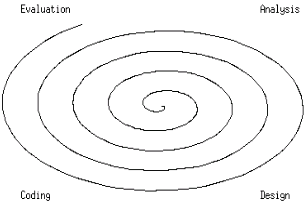
\includegraphics[width=2.5402in,height=1.6799in]{ub-img/ub-img4.png}
\end{center}

{\sffamily\bfseries Figure I-1}
{\sffamily The Spiral Model of Software Development}

\bigskip

\textit{Tight} spirals are better than loose spirals. The more powerful
the prototyping tools, the less time and money spent in early
iterations of development. This translates into either faster
time to market, or a higher quality product. Some prototypes are thrown
away once they have served the purpose of clarifying requirements or
demonstrating some technique. This is OK, but in the spiral model some
prototypes are gradually enhanced until they become the final
production system.

\subsection{Icon: a Very High Level Language for Applications}

Icon is a \index{very high-level language}programming language developed
at the University of Arizona. Icon generalizes its developers' experience
creating an earlier language, \index{SNOBOL4}SNOBOL4. Icon
embodies seminal research ideas, but it is also more fun and
easier to program than other languages.  Most very high-level
languages revel in cryptic syntax, while Icon
is not just more powerful, but often more
\textit{readable} than its competitors. This
gain in expressive power without losing readability is an
addicting result of Icon{\textquotesingle}s elegant design.

The current Arizona Icon, version 9.5, is described in
\textit{The Icon Programming Language}, \textit{3rd edition} by Ralph
and Madge Griswold (1996). Its reference implementation is a
virtual machine interpreter. Icon evolved through many releases
over two decades and is far more capable than it was originally. It is
apparently a finished work.

\subsection{Enter Unicon: More Icon than Icon}

The name Unicon\textbf{\textsuperscript{ }}refers to the descendant of
Icon described in this book and distributed from unicon.org. Unicon is
Icon with portable, platform-independent access to hardware and
software features that have become ubiquitous in modern
applications development, such as objects, networks, and databases.
Unicon is created from the same public domain source code that Arizona
Icon uses, so it has a high degree of compatibility. We were not
free to call it version 10 of the Icon
language, since it was not produced or endorsed by the Icon Project at
the University of Arizona.

Just as the name Unicon frees the Icon Project of all responsibility for
our efforts, it frees us from the requirement of backward
compatibility. While Unicon is almost entirely backward compatible
with Icon, dropping full
compatibility allows us to clear out some dead wood and more
importantly, to make some improvements in the operators that will
benefit everyone at the expense of...no one but the compatibility
police.
This book covers the features of Icon and Unicon together. A
compatibility check list and description of the differences
between Icon and Unicon are given in Appendix D.

\subsection{The Programming Languages Food Chain}

It is interesting to compare Icon and Unicon with the competition.
Mainstream programming languages
such as C, C++, and \index{Java}Java, like the assembler languages that
was mainstream before them, are ideal tools
for writing all sorts of programs, so long as vast amounts of
programmer time are available. Throwing more programmers at a big
project does not work well, and programmers are getting more expensive
while computing
resources continue to become cheaper. These pressures
inexorably lead to the use of higher-level languages and the
development of better design and development methods. Such human
changes are incredibly slow compared to technological changes, but they
are visibly occurring nevertheless. Today, the most
productive programmers are using extra CPU cycles and memory
to reduce the time it takes to develop useful programs.

There is a subcategory of mainstream languages, marketed as \index{rapid
application development}\textit{rapid application development}
languages, whose stated goals seem to address this phenomenon.
Languages such as \index{Visual Basic}Visual Basic or
\index{PowerBuilder}PowerBuilder provide
graphical interface builders and integrated database connectivity,
giving productivity increases in the domain of data entry and
presentation. The value added in these products are in their
programming environments, not their languages. The \index{integrated
development environment}integrated development environments and tools
provided with these languages are to be acclaimed and emulated, but
they do not provide productivity gains that are equally relevant to all
application domains. They are only a partial solution to the needs of
complex applications.

Icon is designed to be easier and faster to program than mainstream
languages. The value it adds is in the expressive power of the language
itself, in the category of very high level languages
that includes \index{Lisp}Lisp,
\index{APL}APL, \index{Smalltalk}Smalltalk, \index{REXX}REXX,
\index{Perl}Perl, \index{Tcl}Tcl, \index{Python}Python, and
\index{Ruby}Ruby; there are
many others. Very high-level languages can be subdivided into
\index{scripting languages}scripting languages and applications
languages. Scripting languages often glue programs
together from disparate sources. They are typically strong in areas
such as multilingual interfacing and file system interactions, while
suffering from weaker expression semantics, typing, scope rules, and
control structures than their applications-oriented cousins.
Applications languages typically originate within a particular
application domain and support that domain with special syntax, control
structures, and data types. Since scripting \textit{is} an application
domain, scripting languages are just one prominent
subcategory of very high-level languages.

Icon is an applications language with roots in text
processing and linguistics. Icon programs tend to be more readable than
similar programs written in other very high-level languages, making
Icon well-suited to the aims of \index{literate
programming}\textit{literate programming}. For example, Icon was used
to implement Norman Ramsey{\textquotesingle}s literate
programming tool \texttt{noweb} (Ramsey, 1994). Literate programming is
the practice of writing programs and their supporting textual
description together in a single document.

Unicon makes the core contributions of Icon useful
for a broader range of applications. This book's many
examples illustrate the range of tasks for which Unicon is well
suited, and these examples are the evidence in
support of Unicon's existence.
Consider using Unicon when one or more of the following conditions are
true. The more conditions that are true, the more you will
benefit from Unicon.

\begin{itemize} \itemsep0pt
\item Programmer time must be minimized.
\item Maintainable, concise source code is desired.
\item The program includes complex data structures or experimental
algorithms.
\item The program involves a mixture of text processing and analysis, custom
graphics, data manipulation, network or file system operations.
\item The program must run on several operating systems and have a
nearly identical graphical user interface with little or no source code
differences.
\end{itemize}

Unicon is not the last word in programming. You probably should not use
Unicon if your program has one or more of the following requirements:

\begin{itemize} \itemsep0pt
\item The fastest possible performance is needed.
\item The program has hard real-time constraints.
\item The program must perform low-level or platform-specific
interactions with the hardware or operating system.
\end{itemize}

Programming languages play a key role in software development.
The Unicon language is a very high level
\index{object-oriented programming}object-oriented language
with a unique combination of expressive power and scalable rapid
development. In this book, many examples from a wide range
of application areas demonstrate how to apply and combine Unicon's
language constructs to solve real-world problems.
It is time to move past the introductions. Prepare to be spoiled by
this language. You may have the same feelings that
Europeans felt when they gave up using Roman numerals and
switched to the Hindu-Arabic number system. {\textquotedbl}This
multiplication stuff isn{\textquotesingle}t that hard
anymore!{\textquotedbl} 


\clearpage
\section{Part I: Core Unicon}

\ \\ \bigskip
\clearpage

\ \\ \bigskip
\clearpage
\bigskip

\chapter{Programs and Expressions}

This chapter presents many of the key features of Unicon, starting
with those it has in common with other popular languages. Detailed
instructions show how to \index{compile}compile and \index{run}run
programs. Soon the examples introduce important ways in which Unicon
is different from other languages. These differences are more than
skin deep. If you dig deeply, you can find dozens of details where
Unicon provides just the right blend of simplicity, flexibility, and
power.  After this chapter, you will know how to
\begin{itemize}\itemsep0pt
  \item edit, compile, and execute Unicon programs
  \item use the basic types to perform calculations
  \item identify expressions that can \index{expression failure}fail, or
    produce multiple results
  \item control the flow of execution using conditionals, looping, and
    procedures
\end{itemize}

\section{Your First Unicon Program}

This section presents the nuts and bolts of writing and running an
Unicon program, after which you will be able to try
the code examples or write your own programs. Before you can run the
examples here or in any subsequent chapter, you must
\index{install}install Unicon on your system. (See Appendix F for
details on downloading and installing Unicon from the Unicon web site,
http://unicon.org.) We are going to be very explicit here,
and assume nothing about your background. If you are an experienced
programmer, you will want to skim this section, and move on to the next
section. If you are completely new to programming, have no fear. Unicon
is pretty easy to learn.

All programs consist of commands that use hardware to obtain or present
information to users, and perform calculations that transform
information into a more useful form. To program a
computer you write a document containing instructions for the computer
to carry out. In Unicon a list of instructions is called
a \index{procedure}\textit{procedure}, and a
\index{program}\textit{program} is a collection of one or more
procedures. In larger programs, groups of related procedures are
organized into classes or packages; these features are presented in
Part II of this book. Unicon programs are text files that may be
composed using any text \index{editor}editor. For the purposes of
demonstration this section describes how to use \index{Ui}Ui, the
program editor and integrated development tool that comes with Unicon.

It is time to begin. Fire up Ui by typing
"ui" from the command line, or launching
the menu item or icon labeled "Unicon," and
type:

\iconcode{
procedure main() \\
\>   write("Hello, amigo!") \\
end
}

Your \index{screen}screen should look something like Figure 1-1. The
large upper area of the window is the editing region where you type
your program code. The lower area of the window is a status region in
which the Ui program displays a message when a command completes
successfully, or when your program has an error. Until you explicitly
name your file something else, a new file has the name
\textsf{noname.icn}. The font Ui uses to display
\index{source code}source code is selectable from the Options menu.

\begin{center}
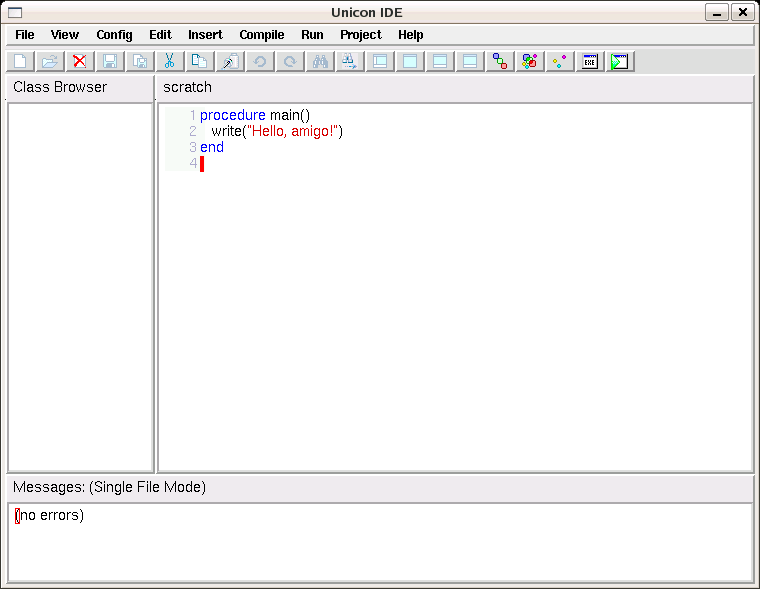
\includegraphics[width=6in,height=4.5953in]{ub-img/ub-img5.png}
\end{center}
\vspace{-0.25cm}{\sffamily\bfseries Figure 1-1:}
{\sffamily Writing an Unicon program using the Ui program.}

\bigskip

The list of instructions that form a \textit{procedure} begins with
the word \texttt{procedure} and ends with the word
\texttt{end}. Procedures have names. After writing a list of
instructions in a procedure you may refer to it by name without
writing out the list again. The \texttt{write()} instruction is just
such a procedure, only it is already written for you; it is built in
to the language. When you issue a \texttt{write()} instruction, you
tell the computer what to write. The details a procedure uses in
carrying out its instructions are given inside the parentheses
following that procedure's name; in this case, \texttt{"Hello, amigo!"}
is to be written.  When you see parentheses after a name in
the middle of a list of instructions, it is an instruction to go
execute that procedure's instructions. Inside the parentheses there
may be zero, one, or many values supplied to that procedure.

Besides writing your program, there are a lot of menu commands that you can use
to control the details of compiling and executing your program within Ui. For
instance, if you select \textbf{Run$\to$Run}, Ui will do the following
things for you.
\begin{enumerate}
  \item Save the program in a file on disk\texttt{.}  All Unicon programs end
    in \texttt{.icn}; you could name it anything you wished, using the
    \textbf{File$\to$SaveAs} command.
  \item Compile the Unicon program from human-readable text to (virtual)
    machine language. To do this step manually, you can select the
    \textbf{Compile$\to$Make executable} command.
  \item Execute the program. This is the main purpose of the \textbf{Run}
    command. Ui performed the other steps in order to make this operation
    possible.
\end{enumerate}
If you type the \texttt{hello.icn} file correctly, the computer should
chug and grind its teeth for awhile, and

\iconcode{
\>   Hello, amigo!
}

\noindent should appear in a window on your screen. This ought to be pretty
intuitive, since the instructions included the line

\iconcode{
\>   write("Hello, amigo!")
}

\noindent in it. That's how to write to the screen.
It's that simple.

The first procedure to be executed when a program runs is called
\texttt{main()}. Every instruction listed in the procedure named
\texttt{main()} is executed in order, from top to bottom, after which
the program terminates. Use the editor to add the following lines right
after the line \texttt{write("Hello,
amigo")} in the previous program:

\iconcode{
\>   write("How are you?") \\
\>   write(7 + 12)
}

\noindent The end result after making your changes should look like this:

\iconcode{
procedure main() \\
\>   write("Hello, amigo!") \\
\>   write("How are you?") \\
\>   write(7 + 12) \\
end
}

Run the program again. This example shows you what a list of
instructions looks like, as well as how easy it is to tell the computer
to do some arithmetic.

{\sffamily\bfseries
Note}

{\sffamily
It would be fine (but not very useful) to tell the computer to add 7 and
12 without telling it to write the resulting value. On seeing the
instruction}

\iconcode{
\>   7 + 12
}

\noindent
the computer would do the addition, throw the 19 away, and go on.

Add the following line, and run it:

\iconcode{
\>   write("7 + 12")
}

This illustrates what quotes are for. Quoted text is taken
literally; without quotes, the computer tries to simplify (do
some arithmetic, or compute the value of what is written), which might
be difficult if the material in question is not an expression!

\iconcode{
\>   write(hey you)
}

\noindent makes no sense and is an error. Add this line, and run it:

\iconcode{
\>   write(7 + "12")
}

The 12 in quotes is taken literally as some text, but that text happens
to be digits that comprise a number, so adding it to another number
makes perfect sense. The computer will not have as much success if you
ask it to add 7 to {\textquotedblleft}amigo{\textquotedblright}. The
computer views all of this in terms of values. A \textit{value} is a
unit of information, such as a number. Anything enclosed in quotes is a
single value. The procedure named \index{write()}\texttt{write()}
prints values on your screen. \textit{Operators} such as \texttt{+}
take values and combine them to produce other values, if it is possible
to do so. The values you give to \texttt{+} had better be numbers! If
you try to add something that doesn't make sense, the
program will stop running at that point, and print an error message.

By now you must have the impression that writing things on your screen
is pretty easy. Reading the \index{keyboard}keyboard is just as easy,
as illustrated by the following program:

\iconcode{
procedure main() \\
\>   write("Type a line ending with
		{\textless}ENTER{\textgreater}:") \\
\>   write("The line you typed was" , read()) \\
end
}

Run the program to see what it does. The procedure named
\index{read()}\texttt{read()} is used to get what the user types. It is
built in to the language. The \texttt{read()} instruction needs no
directions to do its business, so nothing is inside the parentheses.
When the program is run, \texttt{read()} grabs a line from the
keyboard, turns it into a value, and produces that value for use in the
program, in this case for the enclosing \texttt{write()} instruction.

\texttt{The }\texttt{write()} instruction is happy to print out more
than one value on a line, separated by commas. When you run the
program, the \texttt{"the line you typed
was"} part does not get printed until after you type the
line for \texttt{read()} and that instruction completes. The
\texttt{write()} instruction must have all of its directions (the
values inside the parentheses) before it can go about its business.

Now let's try some variations. Can you guess what the
following line will print?

\iconcode{
\>   write("this line says " ,
"read()")
}

The \texttt{read()} procedure is never executed because it is quoted!
Quotes say "take these letters literally, not
as an equation or instruction to evaluate." How about:

\iconcode{
\>   write("this line says , read()")
}

\noindent Here the quotes enclose one big value, which is printed, comma
and all. The directions one gives to a procedure are
\textit{parameters}; when you give a procedure more than one parameter,
separated by commas, you are giving it a
\index{parameter list}\textit{parameter list}. For example,

\iconcode{
\>   write("this value ",
"and this one")
}

\noindent Compile and run the following strange-looking program.
What do you think it does?

\iconcode{
procedure main() \\
\>   while write( "" \~{}== read() ) \\
end
}

This program copies the lines you type until you type an empty line by
pressing Enter without typing any characters first. The
\texttt{""} are used just as usual. They
direct the program to take whatever is quoted literally, and this time
it means literally nothing - an empty line. The operator
\texttt{\~{}==} stands for "\index{not equals}not
equals". It compares the value on its left to the value
on its right, and if they are not equal, it produces the value on the
right side; if they are equal, it \index{expression
failure}\textit{fails} - that is, the {\textquotedblleft}not
equals{\textquotedblright} operator produces no value. If you have
programmed in other languages, this may seem like a strange way to
describe what is usually performed with nice simple Boolean values True
and False. For now, try to take this description at face value; Unicon
has no Boolean type or integer equivalent, it uses a more powerful
concept that we will examine more fully in the chapters that follow.

Thus, the whole expression \texttt{"" \~{}==
read()} takes a line from the keyboard, and if it is not empty, it
produces that value for the enclosing \texttt{write()} instruction.
When you type an empty line, the value \texttt{read()} produces is
equal to \texttt{""}, and \texttt{\~{}==}
produces no value for the enclosing \texttt{write()} instruction, which
similarly fails when given no value. The \index{while}\texttt{while}
instruction is a "\index{loop}loop" that
repeats the instruction that follows it until that instruction fails
(in this case, until there is no more input). There are other kinds of
loops, as well as another way to use \texttt{while}; they are all
described later in this chapter.

So far we've painted you a picture of the Unicon
language in very broad strokes, and informally introduced several
relevant programming concepts along the way. These concepts are
presented more thoroughly and in their proper contexts in the next
sections and subsequent chapters. Hopefully you are already on your way
to becoming an Icon programmer \textit{extraordinaire}. Now it is time
to dive into many of the nuts and bolts that make programming in Unicon
a unique experience.

\section{Command Line Options}

Unicon comes with an IDE, but you can edit programs with any
editor, and compile and run them from your operating
system's command line. This section describes the
Unicon command line tools along with several useful options. The Unicon
compiler executable is named unicon, and to compile the program foo.icn
you would type

\iconcode{
\>   unicon foo
}

\noindent To execute the resulting program, just type

\iconcode{
\>   foo
}

To compile and link a program consisting of several modules, you can
type them all on the command line, as in

\iconcode{
\>   unicon foo bar baz
}

\noindent but often you will want to compile them separately
(using the \texttt{-c} command line option) and link the resulting object
files, called ucode files; their extension is \texttt{.u}

\iconcode{
\>   unicon -c foo\newline \\
\>   unicon -c bar\newline \\
\>   unicon -c baz\newline \\
\>   unicon foo.u bar.u baz.u
}

Some of the other useful command line options include:

\begin{itemize}
\item \texttt{{}-o arg}\ \ \ \ name the resulting output file arg
\item \texttt{{}-x args}\ \ execute the program immediately after linking;
		 this option goes \textit{after} the program filenames
\item \texttt{{}-t}\ \ \ \ turn on tracing
\item \texttt{{}-u}\ \ \ \ produce a warning for undeclared variables
\item \texttt{{}-E}\ \ \ \ output preprocessed source code
\item \texttt{{}-C}\ \ \ \ compile to C code and link
\end{itemize}

These options can be specified in the Ui program under the Compile
menu's Compile Options command. Other options exist;
consult your Unicon and Icon manual pages and platform-specific help
files and release information for more details.

\section{Expressions and Types}

Each \index{procedure}procedure in a Unicon program is a sequence of
\index{expression}\textit{expression}\textit{s.} Expressions are
instructions for obtaining \index{value}values of some
\index{type}type, such as a number or a word; some expressions also
cause side effects, such as sending data to a hardware device.
Simple expressions just read or write a value stored in
memory. More interesting expressions specify a computation that
manipulates zero or more \index{argument}\textit{argument} values to
obtain \index{result}\textit{result} values by some combination of
operators, procedures, or \index{control structure}control structures.

The simplest expressions are \index{literal}\textit{literal}\textit{s},
such as \texttt{2} or \texttt{"hello,
world!"}\texttt{. }These expressions directly specify a
value stored in memory. When the program runs, they do not do any
computation, but rather evaluate to themselves. Literals are combined
with other values to produce interesting results. Each literal has a
corresponding \textit{type}. This chapter focuses on the \index{atomic
types}atomic types. Atomic types represent individual, \index{immutable
values}immutable values. The atomic types in Unicon are
\index{integer}integer and \index{real number}real (floating-point)
numbers, \index{string}string (a sequence of characters), and
\index{cset}cset (a \index{character set}character set). Atomic types
are distinguished by the fact that they have literal values, specified
directly in the program code and represented as data in the compiled
code. Values of other types such as lists are constructed during
execution. Later chapters describe structure types that organize
collections of values, and system types for interacting with the
operating system via files, databases, windows, and network
connections. 

After literals, \index{reference}references to
\index{variable}\textit{variable}\textit{s} are the next simplest form
of expression. Variables are named memory locations that hold values
for use in subsequent expressions. You refer to a variable by its name,
which must start with a letter or underscore and may contain any number
of letters, underscores, or numbers. Use names that make the meaning of
the program clear. The values stored in variables are manipulated by
using variable names in expressions like \texttt{i+j}. This expression
results in a value that is the sum of the values in the variables
\texttt{i} and \texttt{j}, just like you would expect.

Some words may not be used as variable names because they have a special
meaning in the language. These \index{reserved word}\textit{reserved
words} include \texttt{procedure}, \texttt{end},
\texttt{while}, and so on. Other special variables called
\index{keyword}\textit{keywords} start with the ampersand
character (\texttt{\&}) and denote special values. For example, global
variables are initialized to the null value represented by the keyword
\texttt{\&null}\index{null value, \&null}. Other keywords
include \texttt{\&date}, \texttt{\&time}, and so on.
Complete lists of reserved words and keywords are given in Appendix A.

Unlike many languages where you have to state up front
(\textit{declare}) all the variables you are going to use\textit{ }and
specify their data type, in Unicon variables do not have to be declared
at all, and any variable can hold any type of value. However, Unicon
will not allow you to mix incompatible types in an expression. Unicon
is \index{type safe}\textit{type safe}, meaning that every operator
checks its argument values to make sure they are compatible, converts
them if necessary, and halts execution if they cannot be converted.

\section{Numeric Computation}

Unicon supports the usual \index{arithmetic}arithmetic operators on
data types \index{integer}integer and real. Integers are
signed whole numbers of arbitrary magnitude. The real type is a signed
\index{floating point}floating point decimal number whose size on any
platform is the largest size supported by machine instructions,
typically 64-bit double precision values. In addition to
\index{addition}addition (\texttt{+}), \index{subtraction}subtraction
(\texttt{{}-}), \index{multiplication}multiplication (\texttt{*}) and
\index{division}division (\texttt{/}), there are operators for
\index{modulo \%}modulo (\texttt{\%}) and \index{exponentiation
\^{}}exponentiation (\texttt{\^{}}). Arithmetic operators require
numeric operands.

{\sffamily\bfseries
Note}

{\sffamily
Operations on integers produce integers; fractions are truncated, so 8/3
produces 2. If either operand is a real, the other is converted to real
and the result is real, so 8.0/3 is 2.66666...}

As a general rule in Unicon, arguments to numeric operators and
functions are automatically \index{type conversion!type
conversion}converted to numbers if possible, and a \index{run-time
error}run-time error occurs otherwise. The built-in functions
\index{integer(x)}\texttt{integer(x)} and
\index{real(x)}\texttt{real(x)} provide an explicit conversion
mechanism that fails if \texttt{x} cannot be converted to numeric
value, allowing a program to check values without resulting in a
run-time error.

In addition to the operators, built-in functions support several common
\index{numeric operations}numeric operations. The
\index{sqrt(x)}\texttt{sqrt(x)} function produces the square root of x,
and \index{exp(x)}\texttt{exp(x)} raises \textit{e} to the \texttt{x}
power. The value of \index{pi, 3.14... \&pi}\textit{pi} (3.141...) is
available in keyword \texttt{\&pi}, the \index{golden ratio 1.618...,
\&phi}Golden Ratio (1.618...) is available in \index{phi 1.618...,
\&phi}\texttt{\&phi}, and \textit{e} (2.718...) is available in
\index{e, 2.71... \&e}\texttt{\&e}. The \index{log(x)}\texttt{log(x)}
function produces the \index{natural log, log(x)}natural log of
\texttt{x}. The common \index{trigonometric function}trigonometric
functions, such as \index{sin()}\texttt{sin()} and
\index{cos()}\texttt{cos()}\texttt{ }take their angle arguments in
\index{radian}radian units. The \index{min()}\texttt{min(x1, x2, ...)}
and \index{max()}\texttt{max(x1, x2, ...)} routines return minimum and
maximum values from any number of arguments. Appendix A gives a
complete list of built-in functions and operators.

Listing 1-1 shows a simple Unicon program that illustrates the use of
variables in a numeric computation. The line at the beginning is a
comment for the human reader. \index{comment}Comments begin with the
\texttt{\#} character and extend to the end of the line on which they
appear. The compiler ignores them.

\bigskip

{\sffamily\bfseries Listing 1-1}
{\sffamily\bfseries Mystery program}

\iconcode{
\# What do I compute? \\
procedure main() \\
\>   local i, j, old\_r, r \\
\>   i := read() \\
\>   j := read() \\
\>   old\_r := r := min(i, j) \\
\>   while r {\textgreater} 0 do \{ \\
\>\>    old\_r := r \\
\>\>    if i {\textgreater} j then \\
\>\>\>     i := r := i \% j \\
\>\>    else \\
\>\>\>     j := r := j \% i \\
\>\>    \} \\
\>   write(old\_r) \\
end
}

This example illustrates \index{assignment}\textit{assignment}; values
are assigned to (or "stored in") variables
with the \texttt{:=} operator. As you saw in the previous section, the
function \texttt{read()} reads a line from the input and returns its
value. The modulo operator (\texttt{\%}) is an important part of this
program: \texttt{i \% j} is the \index{remainder}remainder when
\texttt{i} is divided by \texttt{j}.

While \index{loop}loops can use a reserved word
\texttt{do} followed by an expression (often a compound expression
in curly braces). The expression following the \texttt{do} is
executed once each time the expression that controls the \texttt{while}
succeeds. Inside the \texttt{while} loop, a
\index{conditional expression}conditional
\index{if-then-else}\texttt{if-then-else} expression is used to select
from two possible actions.

The names of the variables in this example are obscure, and there are no
comments in it other than the one at the top. Can you guess what this
program does, without running it? If you give up, try running it with a
few pairs of positive numbers.

In addition to arithmetic operators, there are \index{augmented
assignment}\textit{augmented assignment} operators. To
increment the value in a variable by 2, these two statements are
equivalent:

\iconcode{
\>   i +:= 2 \\
\>   i := i + 2
}

Augmented assignment works for most \index{binary operator}binary
operators, not just arithmetic. The expression \texttt{i
}\texttt{\textit{op}}\texttt{:= expr} means the same as \texttt{i := i
}\texttt{\textit{op}}\texttt{ expr}.

\section{Strings and Csets}

The non-numeric atomic types in Unicon are character sequences
(\index{string}strings) and \index{character set}character sets
(\index{cset}csets). Icon came from the domain of string
processing, and from it Unicon inherits many sophisticated features for
manipulating strings and performing \index{pattern matching}pattern
matching. This section presents the simple and most common operations.
More advanced operations and examples using strings and csets are given
in Chapter 4.

\index{string!literal}String literals are enclosed in double quotes, as
in \texttt{"this is a string"}, while
\index{cset literal}cset literals are enclosed in single quotes, as in
\texttt{'aeiou'}. Although strings
and csets are composed of characters, there is no
\index{character}character type; a string (or cset) consisting of a
single character is used instead.

Current implementations of Unicon use eight-bit characters, allowing
strings and csets to be composed from 256 unique characters.
\index{ASCII}ASCII representation is used for the lower 128 characters,
except on \index{EBCDIC}EBCDIC systems. The appearance of non-ASCII
values is platform dependent. Like integers, strings can be arbitrarily
large, constrained only by the amount of memory you have on your
system.

Several operators take string arguments. The \index{string!length
(*s)}\texttt{*s} operator gives the \index{length operator (*x)}length
of string \texttt{s}. The expression \index{string!concatenation s1
{\textbar}{\textbar} s2}\texttt{s1{\textbar}{\textbar}s2} produces a
string consisting of the characters in \texttt{s1} followed by
\texttt{s2}. The \index{subscript operator}subscript operator
\index{string!subscript (s[i])}\texttt{s[i]} produces a one-letter
substring of \texttt{s} at the \texttt{i}th position.
\index{string!indexes 1-based}Indices are counted starting from
position 1. If \texttt{i} is nonpositive, it is from the end of the
string, for example \texttt{s[-2]} is the second to the last character
in the string.

Csets support set operators. \index{union (c1 ++ c2)}\texttt{c1++c2}
produces a cset that is the union of \texttt{c1} and \texttt{c2}.
The expression \index{intersection (c1**c2)}\texttt{c1**c2} is the
intersection, while \index{difference (c1 -{}- c2)}\texttt{c1-{}-c2} is
the difference. In addition, several keywords are commonly used
csets. The keywords \index{letters,  \&letters}\texttt{\&letters},
\texttt{\&lcase}, and \texttt{\&ucase} denote the alphabetic
characters, \index{lower case}lower case characters a-z, and
\index{upper case}upper case characters A-Z, respectively, while
\index{digits, \&digits}\texttt{\&digits} is the set from 0-9,
\index{ASCII, \&ascii}\texttt{\&ascii} is the lower 128 characters, and
\index{cset, universal \&cset}\texttt{\&cset} is the set of all (256,
on most implementations) characters.

Many built-in functions operate on strings and csets. Some of the simple
string functions are \index{reverse(x)}\texttt{reverse(s)}, which
produces a string that is the reverse of \texttt{s}, and
\index{trim(s,c)}\texttt{trim(s,c)}, which produces a substring of
\texttt{s} that does not end with any character in cset \texttt{c}.

Functions and operators that require string arguments convert numeric
values to strings automatically, and halt execution with a run-time
error if given a value that cannot be converted to a string.

\section{Goal-directed Evaluation}

\index{goal-directed evaluation}So far, the examples of how
expressions are evaluated have included nothing you
wouldn't find in ordinary programming languages. It is
time to push past the ordinary.
In most conventional languages, each expression always computes
\textit{exactly one} result. If no valid result is possible, a
\index{sentinel value}sentinel value such as -1, NULL, EOF
(\index{end-of-file}end-of-file) or INF (\index{infinity}infinity) is
returned instead. This means that the program must check the return
value for this condition. For example, while reading integers from the
input and performing some operation on them you might do something like
this:

\iconcode{
\>   while (i := read()) \~{}= -1 do \\
\>\>     process(i)
}

This will work, of course, except when you really need to use -1 as a
value! It is somewhat cumbersome, however, even when a sentinel value
is not a problem. Unicon provides a much nicer way to write this type
of code, developed originally in the Icon language. In Unicon,
expressions are \textit{goal-directed}. This means that every
expression when evaluated has a goal of producing results for the
surrounding expression. If an expression succeeds in producing a
result, the surrounding expression executes as intended, but if an
expression cannot produce a result, it is said to \index{expression
failure}fail and the surrounding expression cannot be performed and in
turn fails.

Now take a look at that loop again. If it weren't for
the termination condition, you would not need the
intermediate variable \texttt{i}. If you would like to say:

\iconcode{
\>   process(read())
}

\noindent
your wishes are answered by Unicon; you can indeed write your
program like this. The expression \texttt{read()} tries to produce a
value by reading the input. When it is successful, \texttt{process()}
is called with the value; but when \texttt{read()} cannot get any more
values, that is, at the end of the file, it \textit{fails}. This
failure propagates to the surrounding expression and \texttt{process()}
is not called either. Here is the clincher: control expressions like
\texttt{if} and \texttt{while} don't check for Boolean
(true/false) values, they check for \index{success}success! So our loop
becomes

\iconcode{
\>   while process(read())
}

The \index{do clause}\texttt{do} clause of a \texttt{while} loop is
optional; in this case, the \index{condition}condition does everything
we need, and no \texttt{do} clause is necessary.

Consider the \index{if statement}\texttt{if}\texttt{ }statement that was
used in the earlier arithmetic example:

\iconcode{
\>   if i {\textgreater} j then ...
}

Comparison operators such as \texttt{{\textgreater}} succeed or fail
depending on the values of the operands. This leads to another
question: if an expression like \texttt{i {\textless} 3} succeeds, what
value should it produce? No "true" value is
needed, because any result other than failure is interpreted as
"true." This allows the operator to return
a useful value instead! The \index{comparison operator}comparison
operators produce the value of their right operand when they succeed.
You can write conditions like

\iconcode{
\>   if 3 {\textless} i {\textless} 7 then ...
}

\noindent
that appear routinely in math classes. Other programming languages only
dream about being this elegant. First, Unicon computes \texttt{3
{\textless} i}. If that is true, it returns the value \texttt{i}, which
is now checked with 7. This expression in fact does exactly what
you'd expect. It checks to see that the value of
\texttt{i} is between 3 and 7. (Also, notice that if the first
comparison fails, the second one will not be evaluated.)

\section{Fallible Expressions}

Because some expressions in Unicon can \index{fail!expression}fail to
produce a result, you should learn to recognize such expressions on
sight. These \index{fallible expression}\textit{fallible
expression}\textit{s} control the flow of execution through any piece
of Unicon code you see. When failure is expected it is elegant. When it
is unexpected in your program code, it can be disastrous, causing
incorrect output that you may not notice or, if you are lucky, the
program may terminate with a run-time error.

Some fallible expressions fail when they cannot perform the required
computation; others are \textit{predicates} whose purpose is to fail if
a condition is not satisfied. The subscript and \index{sectioning
operator}sectioning operators are examples of the first category. The
expression \texttt{x[i]} is a \index{subscript operator}subscript
operator that selects element \texttt{i} out of some string or
structure \texttt{x}. It fails if the index \texttt{i} is out of range.
Similarly, the sectioning operator \texttt{x[i:j]} fails if either
\texttt{i} or \texttt{j} are out of range.

The \texttt{read()} function is illustrative of a large number of
built-in functions that can fail. A call to \texttt{read()} fails at
the end of a file. You can easily write procedures that behave
similarly, failing when they cannot perform the computation that is
asked. Unfortunately, for an arbitrary procedure call \texttt{p()}, you
can't tell if it is fallible without studying its
\index{source code}source code or reference documentation. The safest
thing is to expect any procedure call is fallible and check whether it
failed, unless you know it is not fallible or its failure
doesn't matter. Following this advice may avoid many
errors and save you lots of time. In this book we will be careful to
point out fallible expressions when we introduce them.

The less than operator \texttt{{\textless}} is a typical predicate
operator, one that either fails or produces exactly one result. The
unary predicates \index{null test /x}\texttt{/x} and \index{nonnull
test {\textbackslash}x}\texttt{{\textbackslash}x} test a single
operand, succeeding and producing the operand if it is null, or
non-null, respectively. The following binary predicates compare two
operands. The next section presents some additional, more complex
fallible expressions.

\bigskip

\texttt{
{\textless} \ \ \ \ {\textless}= \ \ \ \ {\textgreater}
\ \ \ {\textgreater}= \ \ \ \ \ =
\ \ \ \~{}=}\texttt{\ \ }\ \ \index{numeric comparison}numeric
comparison operators

\texttt{{\textless}{\textless} \ {\textless}{\textless}=
\ {\textgreater}{\textgreater} \ {\textgreater}{\textgreater}= \ ==
\ \~{}==\ \ }\ \ \index{lexical comparison}lexical (alphabetic)
comparison

\ \ \ \ \ \ \ \ \texttt{=== \ \ \ \ \ \ \ \ \~{}===}\ \ \ \ \ \ \ \ \ \ \ \ \ \ \ \ \index{reference
comparison}reference comparison

\section[Generators]{Generators}

So far we have seen that an expression can produce no result (failure)
or one result (success). In general, an expression can produce any
number of results: 0, 1, or many. Expressions that can produce more
than one result are called \index{generator}\textit{generators}.
Consider the task of searching for a substring within a string:

\iconcode{
\>   find("lu",
"Honolulu")
}

In most languages, this would return one of the substring matches,
usually the first position at which the substring is found. In Unicon,
this expression is a generator, and can produce \textit{all} the
positions where the substring occurs. If the surrounding expression
only needs one value, as in the case of an if test or an assignment,
only the first value of a generator is produced. If a generator is part
of a more complex expression, then the return values are produced in
sequence until the whole expression produces a value.

Let us look at this example:

\iconcode{
\>   3 {\textless} find("or",
"horror")
}

The first value produced by \index{find()}\texttt{find()} is 2, which
causes the \texttt{{\textless}}\texttt{ }operation to fail. Execution
then resumes the call to \texttt{find()}, which produces a 5 as its
next value, and the expression succeeds. The value of the expression is
the first position of the substring greater than 3.

The most obvious generator is the \index{alternation operator (
{\textbar} )}alternation operator \texttt{{\textbar}}. The expression

\iconcode{
\>   expr1 {\textbar} expr2
}

\noindent
produces its left-hand side followed by its right-hand side, if needed
by the surrounding expression. This can perform many computations quite
compactly. For example,

\iconcode{
\>   x = (3 {\textbar} 5)
}

\noindent
checks to see if the value of \texttt{x} is 3 or 5. More complex
expressions follow logically:

\iconcode{
\>   (x {\textbar} y) = (3 {\textbar} 5)
}

\noindent
checks to see if either \texttt{x} or \texttt{y} has the value 3 or
5. It is the Unicon equivalent of C's

\iconcode{
\>   (x == 3) {\textbar}{\textbar} (x == 5) {\textbar}{\textbar} (y ==
3) {\textbar}{\textbar} (y == 5)
}

In understanding Unicon code, it helps if you identify the
generators, if there are any. In addition to the alternation operator
\texttt{{\textbar}} and the function \texttt{find()}, there are a few
other generators in Icon's built in repertoire of
operators and functions. We mention them briefly here, so you can be on
the lookout for them when reading code examples.

The expression \texttt{i }\index{to, generator}\texttt{to j} is a
generator that produces all the values between \texttt{i} and
\texttt{j.} The expression \texttt{i to j }\index{to-by,
generator}\texttt{by k} works similarly, incrementing each result by
\texttt{k}; \texttt{i}, \texttt{j}, and \texttt{k} must all be integer
or real numbers, and \texttt{k} must be non-zero. The expression
\texttt{i to j} is equivalent to \ \ \ \ \ \ \texttt{i to j by 1}. The
unary \index{generate operator "!x}\texttt{!} operator is a generator
that produces the elements of its argument. This works on every type
where it makes sense. Applied to a string, it produces all its
characters (in order). Sets, tables, lists, or records produce the
members of the structure.

Generators get resumed for more results as needed in order for the
surrounding expression to succeed, and this may propagate through many
levels of nested enclosing expressions. However, special expressions
called \index{bounded experssions}\textit{bounded expressions} will
never resume their generator subexpressions. For example, the
conditional expressions used in \texttt{if} and \texttt{while} are
never resumed if they succeed; if they produce a result the then-branch
or the loop body is executed, and if that code fails, it does not cause
generators in the conditional to be resumed. Those bounded conditional
expressions are re-evaluated starting from scratch if execution comes
their way again. Another popular bounded expression is the semi-colon
operator. The expression \texttt{expr1 ; expr2 }evaluates the two
expressions in order, and bounds the first expression, so you
don't have to worry about backtracking into it if the
second expression fails.

\section{Iteration and Control Structures}

You have already seen two control structures in Unicon: the
\texttt{if} and the \texttt{while} loop, which test for
\index{success}success.  Unicon has several other control structures
that vary in complexity and usefulness. Unicon is expression-based,
and all control structures are expressions that can be used in
surrounding expressions if desired. The big difference between control
structures and ordinary operators or procedures is that ordinary
operators and procedures don't execute until their arguments have been
evaluated and produced a result; they don't execute at all if an
argument fails. In contrast, a control structure uses one of its
arguments to decide whether (or how many times) to evaluate its other
arguments.

Since control structures are expressions, they may produce a result
for a surrounding expression. For example, the result of an
\texttt{if} expression is the result of either its \texttt{then} part
or its \texttt{else} part, whichever one was selected. On the other
hand, a loop executes until its test fails, after which there is no
meaningful result for it to produce; loops usually fail as far as
surrounding expressions are concerned.

The \index{control structure}control structure \index{every}\texttt{every}
processes the entire sequence of values produced by a generator. The expression

\iconcode{
\>   every \textit{expr1} do \textit{expr2}
}

\noindent
evaluates \texttt{\textit{expr2}} for each result generated by
\texttt{\textit{expr1}}. This loop looks similar enough to a
\texttt{while} loop to confuse people at first. The difference is that
a \texttt{while} loop re-evaluates \texttt{\textit{expr1}} from scratch
after each iteration of \texttt{\textit{expr2}}, but \texttt{every}
\textit{resumes} \texttt{\textit{expr1}} for an additional result where
it left off the last time through the loop. Using a generator to
control a \texttt{while} loop makes no sense; the generator will
restart each iteration, which may give you an infinite loop. Similarly,
\textit{not} using a generator to control an \texttt{every} loop also
makes no sense; if \texttt{\textit{expr1}} is not a generator the loop
body executes at most one time.

The classic example of \texttt{every} is a loop that generates the number
sequence from a \texttt{to} expression, assigning the number to a variable that
can be used in \texttt{\textit{expr2}}. In many languages these are called
``for'' loops. A \index{for loop}for loop in Unicon is written like this:

\iconcode{
\>   every i := 1 to 10 do write(i)
}
\noindent
Of course, \texttt{every} and \texttt{to} are not limited to this BASIC-style
for loop. Generators are more flexible; the for loop
above looks clumsy when compared with the equivalent

\iconcode{
\>   every write(1 to 10)
}

\noindent
A generator operand to a non-generator forms a generator. The enclosing
non-generator (such as \texttt{write()}) is re-run each time
the generator suspends and resumes.

Unicon's \texttt{every} keyword generalizes the concept of
\index{iterator}\textit{iterators} found in other languages.  Iterators are
special control structures that walk through a collection of data. Instead of
being a special feature, in Unicon iterators are just one of many ways to
utilize generators. The \index{sequence of results}sequence of results from an
expression does not have to be stored in a structure to iterate over them. The
sequence of results does not even have to be finite; many
\index{generator}generator expressions produce an infinite sequence of results,
as long as the surrounding expression keeps asking them for more. Here is
another example of how \texttt{every} expressions are more flexible than for
loops. The expression

\iconcode{
\>   every f(1 {\textbar} 4 {\textbar} 9 {\textbar} 16 {\textbar} 25
{\textbar} 36)
}

\noindent
executes the function \texttt{f} several times, passing the first few
square numbers as parameters. A shorter equivalent that uses the power
operator (\texttt{\^{}}) is \texttt{every f((1 to 6)\^{}2)}. An example
in the next section shows how to generalize this to work with all the
squares.

The \texttt{if}, \texttt{while}, and \texttt{every} expressions are
Unicon's primary control structures. Several other
control structures are available that may be more useful in certain
situations. The loop

\iconcode{
\>   \index{until}until \textit{expr1} do \textit{expr2}
}

\noindent is \texttt{while}'s evil twin, executing
\texttt{\textit{expr2}} as long as \texttt{\textit{expr1}}
\index{expression failure}fails; on the other hand

\iconcode{
\>   \index{repeat loop}repeat \textit{expr}
}

\noindent is an infinite loop, executing \texttt{\textit{expr}}
over and over.

There are also variations on the \texttt{if} expression introduced
earlier for conditional execution. First, the \texttt{else} branch is
optional, so you can have an \texttt{if} expression that does nothing
if the condition is not satisfied. Second, there is a special control
structure introduced for the common situation in which several
alternatives might be selected using a long sequence of \texttt{if ...
else if ... else if ...} expressions. The \index{case expression} \texttt{case}
expression replaces these chains of \texttt{if} expressions with the syntax:

\iconcode{
\>   case \textit{expr} of \{ \\
\>   \textit{branch1}: \textit{expr1} \\
\>   \textit{branch2}: \textit{expr2} \\
\>   ... \\
\>   default: \textit{expr}\textit{\textsubscript{i}} \\
\>   \}
}

When a \texttt{case} expression executes, the \texttt{\textit{expr}} is
evaluated, and compared to each branch value until one that matches
exactly is found, as in the binary equality operator \texttt{===}.
Branch expressions can be generators, in which case every result from
the branch is compared with \texttt{\textit{expr}}. The default branch
may be omitted in case expressions for which no action is to be taken
if no branch is satisfied.

When we introduced the \texttt{repeat} loop, you probably were
wondering how to exit from the loop, since most applications do not
run forever.  One answer would be to call one of the built-in
functions that terminate the entire program when it is time to get out
of the loop.  The \texttt{exit()}, \texttt{stop()}, and
\texttt{runerr()} functions all serve this valuable purpose; their
differences are described in Appendix A.

A less drastic way to get out of any loop is to use the
\index{break expression}\texttt{break} expression:

\iconcode{
\>   break \textit{expr}
}

This expression exits the nearest enclosing loop; \texttt{\textit{expr}}
is evaluated outside the loop and treated as the value produced by
executing the loop. This value is rarely used by the surrounding
expression, but the mechanism is very useful, since it allows you to
chain any number of breaks together, to exit several levels of loops
simultaneously. The \texttt{break} expression has a cousin called
\texttt{next} that does not get out of a loop, but instead skips the
rest of the current iteration of a loop and begins the next iteration
of the loop.


\section{Procedures}

\index{procedure}Procedures are a basic building block in most
languages. Here is an example of an ordinary procedure. This one
computes a simple polynomial, $a x^2 + b x + c$.

\iconcode{
procedure poly(x,a,b,c) \\
\>   return a * x\^{}2 + b * x + c \\
end
}

\subsection*{Parameters}

Procedure \index{parameter}parameters are passed by value except for
\index{structure types}structured data types, which are passed by
\index{reference}reference. This means that when you pass in a string,
number, or cset value, the procedure gets a \textit{copy} of that
value; any changes the procedure makes to its copy will not be
reflected in the calling procedure. On the other hand, structures that
contain other values, such as lists, tables, records, and sets are not
copied. The procedure being called gets a handle to the original value,
and any changes it makes to the value will be visible to the calling
procedure. Structure types are described in the next chapter.

When you call a procedure with \index{parameters!wrong number}too many
parameters, the extras are discarded. This feature is valuable for
prototyping but can be dangerous if you aren't
careful! Similarly, if you call a procedure with too few parameters,
the remaining variables are assigned the null value, \texttt{\&null}.
The null value is also passed as a parameter if you omit a parameter.

Now it is time to describe the unary operators \texttt{{\textbackslash}}
and \texttt{/}. These operators test the expression against the null
value. The expression \index{null test /x}\texttt{/}\texttt{\textit{x}}
succeeds and returns \texttt{\textit{x}} if the value is the null
value. This can be used to assign default values to procedure
arguments: Any arguments that have a null value can be tested for and
assigned a value. Here's an example:

\iconcode{
procedure succ(x, i) \\
\>   /i := 1 \\
\>   return x + i \\
end
}

If this procedure is called as \texttt{succ(10)}, the missing second
parameter, \texttt{i}, is assigned the null value. The forward slash
operator then tests \texttt{i} against the null value, which succeeds;
therefore the value 1 is assigned to \texttt{i}.

The backward slash checks if its argument is non-null. For example, this
will write the value of \texttt{x} if it has a non-null value:

\iconcode{
\>   write("The value of x is ",
	{\textbackslash}x)
}

If \texttt{x} does in fact have the null value, then \index{nonnull test
{\textbackslash}x}\texttt{{\textbackslash}x} will fail, which will mean
that the \texttt{write()} procedure will not be called. If it helps you
to not get these two mixed up, a slash pushes its operand
"up" for non-null, and
"down" for a null value.

The procedure \texttt{succ()} shows one way to
specify a default value for a parameter. The built-in functions use
such default values systematically to reduce the number of parameters
needed; consistent defaults for entire families of functions make them
easy to remember. Another key aspect of the built-in operations is
implicit type conversion. Arguments to built-in functions and operators
are converted as needed.

\index{default, parameter}Defaulting and \index{type conversion}type
conversion are so common and so valuable in Unicon that they have their
own syntax. Parameter names may optionally be followed by a coercion
function (usually the name of a built in type) and/or a default value,
separated by colons. These constructs are especially useful in
enforcing the public interfaces of library routines that will be used
by many people.

\iconcode{
procedure succ(x:integer, i:integer:1) \\
end
}

\noindent
This parameter declaration is a more concise equivalent of

\iconcode{
procedure succ(x, i) \\
\>   x := integer(x) {\textbar} runerr(101, x) \\
\>   /i := 1 {\textbar} i := integer(i) {\textbar} runerr(101, i) \\
end
}

\subsection*{Variables and scopes}

\index{Variable}Variable names used as parameters are fundamentally different
from procedure names. The \index{scope,}\textit{scope} of parameters is limited
to the body of a single procedure, while procedure names are visible to the
entire program.  Parameters and procedures are special forms of two basic kinds
of variables in Unicon: local variables and global variables.

The scope of \index{global variables}global variables, including
procedure names, consists of the entire program. Their value is stored
in memory for the entire execution of the program. There are two kinds
of \index{local variables}local variables; both introduce names that
are defined only within a particular procedure. Regular local
variables are created when a procedure is called, and destroyed when a
procedure fails or returns a result; a separate copy of regular local
variables is created for each call. \index{static variables}Static
local variables are global variables whose names are visible only
within a particular procedure; a single location in memory is shared
by all calls to the procedure, and the last value assigned in one call
is remembered in the next call.

Variables do not have to be declared, and by default they are \textit{local}.
To get a global variable, you have to declare it outside any procedure with a
declaration like this:

\iconcode{
global MyGlobal
}

Such a declaration can be before, after, or in between procedures within
a program source file, but cannot be inside a procedure body. Of
course, another way to declare a global variable is to define a
procedure; this creates a global variable initialized with the
appropriate procedure value containing the procedure's
instructions.

Regular and static local variables may be declared at the top of a
procedure body, after the parameters and before the code starts, as in
the following example:

\iconcode{
procedure foo() \\
\>   local x, y \\
\>   static z \\
\>   ... \\\
end
}

Each declared local variable name may be followed by a \texttt{:=} and
an \textit{initializer} expression that specifies the
variable's initial value. Without an initializer,
variables start with the value \texttt{\&null}. Although
you do not have to declare local variables, large programs,
library code or multi-person projects should declare
all local variables. If you don't, and some other part
of the code introduces a global variable by the same name as your
undeclared local, your variable will be interpreted as a
\index{reference}reference to the global. To help avoid this
problem, the \texttt{{}-u} command line option to the
\index{compiler}compiler causes \index{undeclared variables}undeclared
local variables to produce a compilation error message.

A procedure body can begin with an \index{initial
clause}\texttt{initial} clause, which executes only the first time
the procedure is called. The \texttt{initial} clause is mainly used
to initialize static variables in ways that aren't
handled by initializers. For example, the following procedure returns
the next number in the Fibonacci sequence each time it is
called, using static variables to remember previous results in the
sequence between calls.

\iconcode{
procedure fib() \\
static x,y \\
local z \\
initial \{ \\
\>   x := 0 \\
\>   y := 1 \\
\>   return 1 \\
\>   \} \\
\>   z := x + y \\
\>   x := y \\
\>   y := z \\
\>   return z \\
end
}

\subsection*{Writing your own generators}

\index{generator}When a procedure returns a value, the procedure and its
regular local variables cease to exist. But there are expressions that
don't disappear when they produce a value: generators!
You can create your own generators by writing procedures that use
\texttt{suspend} instead of \texttt{return. suspend} is different from
\texttt{return} in that it saves the point of execution within the
procedure; if another value is required by the calling expression, the
generator continues execution from where it previously left off.

Here is a procedure to generate all the squares. Instead of using
multiplication, it uses addition to demonstrate generators! The code
uses the fact that if we keep adding successive odd numbers, we get the
squares.

\iconcode{
procedure squares() \\
\>   odds := 1 \\
\>   sum := 0 \\
\>   repeat \{ \\
\>   \ \ \ suspend sum \\
\>   \ \ \ sum +:= odds \\
\>   \ \ \ odds +:= 2 \\
\>   \} \\
end
}

To perform a computation on the squares, we can use it in an
\texttt{every} statement:

\iconcode{
\>   every munge(squares())}

{\sffamily\bfseries
Warning}

{\sffamily
This is an infinite loop! (Do you know why? Whether \texttt{munge()} succeeds or
fails, \texttt{every} will always resume \texttt{squares()} for another result
to try; \texttt{squares()} generates an infinite result sequence.)}

The \index{expression failure}\texttt{fail} expression makes the
procedure fail. Control goes to the calling procedure, returning
no value, and the procedure call ceases to exist; it cannot be
resumed. A procedure also fails implicitly when control flows off the
end of the procedure's body.

Here is a procedure that produces all the non-blank characters of a
string, but bails out if the character \texttt{\#} is reached:

\iconcode{
procedure nonblank(s) \\
\>   every c := !s do \{ \\
\>   \ \ \ if c == "\#" then fail \\
\>   \ \ \ if c \~{}== " " then suspend c \\
\>   \} \\
end
}

\subsection*{Recursion}

\index{recursion}A recursive procedure is one that calls itself,
directly or indirectly. There are many cases where it is the most
natural way of solving the problem. Consider the famous
"Towers of \index{Hanoi}Hanoi" problem.
Legend has it that when the universe was created, a group of monks
in a temple in some remote place were presented with a problem.
There are three diamond needles, and on one of them is a
\index{stack}stack of 64 golden disks all of different sizes, placed in
order with the largest one at the bottom and the smallest on top. All
the disks are to be moved to a different needle under the conditions
that only one disk may be moved at a time, and a larger disk can never
be placed on a smaller disk. When the monks finish this task, the
universe will come to an end.

How can you move the \textit{n} smallest disks? If \textit{n} is
1, just move it. Since it's the
smallest, this will not violate the condition. If \textit{n} is
greater than 1, here's what we can do: first, move the
\textit{n-1} upper disks to the intermediate needle, then transfer the
\textit{n}th disk, then move the \textit{n-1} upper disks to the
destination needle. This whole procedure does not violate the
requirements either (satisfy yourself that such is the case).

Now write the procedure \texttt{hanoi(n)} that computes this algorithm.
The first part is simple: if you have one disk, just move it.

\iconcode{
procedure hanoi(n, needle1:1, needle2:2) \\
\>   if n = 1 then write("Move disk from ",
needle1, " to ", needle2)
}

\noindent
Otherwise, perform a recursive call with \textit{n-1}. First, to find
the spare needle we have:

\iconcode{
\>   other := 6 - needle1 - needle2}

Now move the \textit{n-1} disks from \texttt{needle1} to \texttt{other},
move the biggest disk, and then move the \textit{n-1} again. The
needles are passed as additional parameters into the recursive calls.
They are always two distinct values out of the set \{1, 2, 3\}.

\iconcode{
\>   hanoi(n-1, needle1, other) \\
\>   write("Move disk from ", needle1,
" to ", needle2) \\
\>   hanoi(n-1, other, needle2)
}

\noindent
That's it! You're done. Listing
1-2 contains the complete program for you to try:

\bigskip

{\sffamily\bfseries Listing 1-2}
{\sffamily\bfseries Towers of Hanoi}

\iconcode{
procedure main() \\
\>   write("How many disks are on the towers of
Hanoi?") \\
\>   hanoi(read()) \\
end \\
procedure hanoi(n:integer, needle1:1, needle2:2) \\
local other \\
\>   if n = 1 then write("Move disk from ",
needle1, " to ", needle2) \\
\>   else \{ \\
\>   \ \ \ other := 6 - needle1 - needle2 \\
\>   \ \ \ hanoi(n-1, needle1, other) \\
\>   \ \ \ write("Move disk from ", needle1, " to ", needle2) \\
\>   \ \ \ hanoi(n-1, other, needle2) \\
\>   \} \\
end
}

\noindent
Turn on \index{tracing}tracing see how this program works.
To enable tracing, \index{compile}compile your program with a
\texttt{{}-t} option, or assign the keyword \texttt{\&trace} a non-zero
number giving the depth of calls to trace. Setting \texttt{\&trace} to
-1 will turn on tracing to an infinite depth.

To move \textit{n} disks,
\textit{2}\textit{\textsuperscript{n}}\textit{ - 1} individual disk
movements will be required. If the monks move one disk a second, it
will take \textit{2}\textit{\textsuperscript{64}}\textit{ - 1}
seconds, or about 60 trillion years. Wikipedia has listed the age of
the universe at around 13.75 billion years. It seems unlikely
that we need worry about the monks finishing their task!

\section*{Summary}

In this chapter you have learned:

\begin{itemize}\itemsep0pt
\item Unicon is an expression-based language organized as a set of
procedures starting from a procedure called \texttt{main()}.

\item Unicon has four atomic types: arbitrary precision integers, real
numbers, arbitrary length strings of characters, and character sets.

\item There is no Boolean concept in Unicon; instead, control is driven
by whether an expression succeeds in producing a result or
\index{fail}fails to do so. This eliminates the need for most
\index{sentinel value}sentinel values, shortening many expressions.

\item \index{generator}Generator expressions can produce multiple
results as needed by the surrounding expression in order for it to
produce results.

\item Procedure parameters are passed by value for atomic types, and by
reference for all other data types. Unicon features extensive argument
defaults and automatic type coercion throughout its built-in function
and operator repertoire.

\item Unicon has two scope levels: global and local. Undeclared
variables are implicitly defined to be local.
\end{itemize}

\bigskip


\chapter{Structures}

The examples in the previous chapter employed data types whose values
are \textit{immutable}. For example, all operations that manipulate
numbers and strings compute new values, rather than modify existing
values. This chapter presents structured types that organize and store
collections of arbitrary (and possibly mixed) types of values. When you
complete this chapter, you will understand how to use these types.
\begin{itemize}
  \item Tables associate their elements with key values for rapid lookup.
  \item Lists offer efficient access by position as well as by
    \index{stack}stack or \index{queue}queue operations.
  \item Records store values using a fixed number of named fields.
  \item Sets support operations such as union and intersection on groups
    of elements.
  \item Using structures to represent \index{tree}trees, graphs, and
    matrices.
\end{itemize}
There are several structure types that describe different basic
relationships between values. The philosophy of structures in Unicon is
to provide built-in operators and functions for common organization and
access patterns - the flexible "super glue"
that is needed by nearly all applications. Their functionality is
similar to the C++ Standard Template Library or generic classes in
other languages, but Unicon's structure types are much
simpler to learn and use, and are well supported by the expression
evaluation mechanism described in the previous chapter.

All structure types in Icon share many aspects in common, such as the
fact that structures are \index{mutable values}\textit{mutable}. The
values inside them may change. In that respect, structures are similar
to a collection of variables that are bundled together. In many cases,
Unicon's structure types are almost interchangeable!
Operators like subscripts and built-in functions such as
\index{insert()}\texttt{insert()}\texttt{ }are defined consistently for
many types. Code that relies on such operators is
\index{polymorphism}\textit{polymorphic}: it may be used with multiple
structure types in an interchangeable way.

For both the structures described in this chapter and the strings
described in the next chapter, be aware that Unicon performs
\index{automatic storage management}automatic storage management, also
known as \index{garbage collection}garbage collection. If you have used
a language like C or C++, you know that one of the biggest headaches in
writing programs in these languages is tracking down bugs caused by
\index{memory allocation}memory allocation, especially dynamic heap
memory allocation. Unicon transparently takes care of those issues for
you.

Another big source of bugs in languages like C and C++ are
\index{pointer}pointers, values that contain raw \index{memory
addresses}memory addresses. Used properly, pointers are powerful and
efficient. The problem is that they are easy to use incorrectly by
accident; this is true for students and practicing software engineers
alike. It is easy in C to point at something that is off-limits, or to
trash some data through a pointer of the wrong type.

Unicon has no pointer types, but all structure values implicitly
use pointer semantics. A \index{reference}\textit{reference} is a
pointer for which type information is maintained and safety is
strictly enforced. All structure values are references to
data that is allocated elsewhere, in a memory region known as
the \index{heap}heap. You can think of a reference as a safe
pointer: the only operations it supports are copying the pointer, or
dereferencing it using an operation that is defined for its type.

Assigning a structure to a \index{variable}variable, or passing it as a
\index{parameter}parameter, gives that variable or parameter a copy of
the reference to the structure but does not make a copy of the
structure. If you want a copy of a structure, you call the function
\texttt{copy(x)}, which makes a "shallow"
copy of a single table, list, record, or set. If that structure
contains references to other structures as its elements, those
substructures are not copied by \texttt{copy()}. To copy a
"deep" structure (lists of lists, tables of
records, etc.) you can use the procedure \texttt{deepcopy()} that is
given as an example later in this chapter.

\section{Tables}

\index{table data type}Tables are unordered collections of values that
are accessed using \index{associative memory}associated \index{keys,
table}\textit{keys}. They are Unicon's most versatile
type. All of the other structure types can be viewed as special cases
of tables, optimized for performance on common operations. Most
operations that are defined for tables are defined for other structure
types as well.

\index{table lookup}Subscripts are used for the primary operations of
associating keys with values that are inserted into the table, and then
using keys to look up objects in the table. The \texttt{table()}
function creates a new empty table. For example, the lines

\iconcode{
T := table() \\
T["hello"] :=
"goodbye"
}

\noindent
create a new table, and associate the key \texttt{"hello"} with the value
\texttt{"goodbye"}. The \texttt{table()} function takes one optional argument:
the \index{default value!table}default value to return when lookup
\index{expression failure}fails. The default value of the default value is
\texttt{\&null}, so after the above example, \texttt{write(T["goodbye"])} would
write an empty line, since \texttt{write()} treats a null argument the same as
an empty string, and \texttt{write()} always writes a newline.  Assigning a
value to a key that is not in the table inserts a value into the table. This
occurs in the second line of the example above, so \texttt{write(T["hello"])}
writes out \texttt{"goodbye"}.

Subscripts are the primary operation on tables, but there are several
other useful operations. The \index{insert()!table}\texttt{insert(T,
k}\texttt{\textsubscript{1}}\texttt{,
x}\texttt{\textsubscript{1}}\texttt{,
k}\texttt{\textsubscript{2}}\texttt{,
x}\texttt{\textsubscript{2}}\texttt{, ...)} function adds new key-value
pairs to \texttt{T}. The \index{delete()!table}\texttt{delete(T,
k}\texttt{\textsubscript{1}}\texttt{,
k}\texttt{\textsubscript{2}}\texttt{, ...)} function deletes values
from \texttt{T} that correspond to the supplied keys.
Icon's unary \texttt{*} operator produces the size of
its argument; for a table, \index{table!length *T}\texttt{*T} is the
number of key-value pairs in the table. Unary \texttt{!} generates
elements from a collection; for a table, \texttt{!T} generates the
values stored in the table. Unary \texttt{?} is the random operator;
for a table, \texttt{?T} produces a random value stored in the table.
Both unary \texttt{!} and \texttt{?} produce values stored in a table,
not the keys used to lookup values.

Function \index{member()!table}\texttt{member(T, k)} succeeds if
\texttt{k} is a key in \texttt{T} and fails otherwise. Function
\index{key()!table}\texttt{key(T)} generates the keys that have
associated values. The following example prints word counts for the
input (assuming \texttt{getword()} generates words of
interest): 

\iconcode{
wordcount := table(0) \\
every word := getword() do wordcount[word] +:= 1 \\
every word := key(wordcount) do write(word, " ", wordcount[word])
}

The default value for the table is 0. When a new word is inserted, the
default value gets incremented and the new value (that is, 1) is stored
with the new word. Tables grow automatically as new elements are
inserted.

\section{Lists}

\index{list data type}Lists are dynamically sized ordered
collections of values. They are accessed by subscripts, with indexes
starting at 1. You can also insert or remove
elements from the beginning, middle, or end of the list. Lists take the
place of \index{array}arrays, \index{stack}stacks, \index{queue}queues,
and \index{deque}deques found in other languages and data structures
textbooks.

A list is created by calling the function \index{list()}\texttt{list()}, which
takes optional parameters for the lists's initial size and the initial value
given to all elements of the list.  By default \texttt{list()} creates an empty
list. Alternatively, you can create a list by enclosing a comma-separated
sequence of values in square brackets:

\iconcode{
L := ["linux", 2.0,
	"unix"]
}

Lists are dynamic. Lists grow or shrink as a result
of stack and queue operations. The \index{push()}\texttt{push()} and
\index{pop()}\texttt{pop()} functions add and remove elements from the
front of a list, while \index{put()}\texttt{put()} and
\index{pull(L)}\texttt{pull()} add and remove elements at the end of
the list. In addition,
{\em \index{insert()!list}\texttt{insert(L, i, x)} inserts
\texttt{x} at position \texttt{i}, and
\index{delete()!list}\texttt{delete(L, i)}\texttt{ }deletes the element
at position \texttt{i}.\/}
The expression \texttt{[]} is another
way to create an \index{empty list}empty list; it is equivalent to
calling \texttt{list()} with no arguments.
The previous list could have been constructed one element at
a time with the following code.
{\em \texttt{put()} accepts a variable number of arguments\/}.

\iconcode{
L := [ ] \\
put(L, "linux") \\
put(L, 2.0) \\
put(L, "unix")
}

Elements of the list can be obtained either through list manipulation
functions or by subscripting. Given the list \texttt{L} above, in the
following code the first line writes
\texttt{"unix"} while the second line moves
the first element to the end of the list.

\iconcode{
write(L[3]) \\
put(L, pop(L))
}

There is no restriction on the kinds of values that may be stored in a
list. For example, the elements of a list can themselves be lists. You
can create lists like

\iconcode{
L := [[1, 2, 3], [4, 5, 6], [7, 8, 9]]}

\noindent and index them with multiple subscripts. \texttt{L[2][3]} is
equivalent to \texttt{L[2,3]} and yields the value 6 in this example. 

Lists also support several common operators. The operator
\index{list!size (*L)}\texttt{*L} produces the size of list \texttt{L}.
The operators \texttt{!L} and \texttt{?L} generate the elements of
\texttt{L} in sequence, and produce a single random element of
\texttt{L}, respectively. The following procedure uses the unary
\texttt{!} operator to sum the values in list \texttt{L}, which must be
numbers.

\iconcode{
procedure sum(L) \\
\>   total := 0 \\
\>   every total +:= !L \\
\>   return total \\
end
}

Comparing the two, lists are like tables with boring keys: the
positive integers starting from 1. {\em Function \texttt{member(L, k)}
succeeds if \texttt{0 {\textless} integer(k) {\textless}= *L}\/}, while
\texttt{key(L)} is equivalent to the expression \texttt{1 to *L}. List
indexes are contiguous, unlike table keys, and so lists can support a
\index{slice!list L[i:j]}\textit{slice} operator to produce a sublist,
given a pair of indexes to mark the bounds. The \texttt{L[i:j]}
expression produces a new list that contains a copy of the elements in
\texttt{L} between positions \texttt{i} and \texttt{j}. The
\texttt{L[i+:j]} expression is equivalent to \texttt{L[i:i+j]}. List
concatenation is another valuable operator. The \index{list
concatenation!L1 {\textbar}{\textbar}{\textbar} L2}\texttt{L1
{\textbar}{\textbar}{\textbar} L2} expression produces a new list whose
elements are a copy of the elements in \texttt{L1} followed by a copy
of the elements in \texttt{L2}.

\section{Records}

A \index{record}record is a fixed-sized, ordered collection of values
whose elements are accessed using user-defined named \textit{fields}. A
record is declared as a global name that introduces a new type with a
corresponding \index{constructor!record}constructor procedure, as in
the following example. The field names are a comma-separated list of
identifiers enclosed in parentheses.

\iconcode{
record complex(re, im)}

Record \index{instance!record}\textit{instances} are created using a
constructor procedure with the name of the record type. The
fields of an instance are accessed by name using dot notation or string
subscript, or by integer index subscript. You can use records as
records, or as special tables or lists with
a constant size and fixed set of keys.

\texttt{member(R,s)} tests whether \texttt{s} is a field in \texttt{R};
\texttt{key(R)} generates \texttt{R}'s field names.
Functions like \texttt{insert()}, or \texttt{push()} are not supported
on records, since they change the size of the structure that they
modify. Here is a demonstration of record operations.

\iconcode{
a := complex(0, 0) \\
b := complex(1, -1) \\
if a.re = b.re then write("not likely") \\
if a["re"] = a[2] then
write("a.re and a.im are equal")
}

Unicon provides a mechanism for constructing new record types on the
fly, described in Chapter 6, as well as the ability to declare classes,
which are new data types that form the building blocks for
object-oriented programs, described starting in Chapter 9. Records are
closely related to classes and objects: they can be considered to be an
optimized special case of objects that have no methods. \ 

\section{Sets}

A \index{set data type}set is an unordered collection of values with the
uniqueness property: an element can only be present in a set once. The
function \texttt{set(x...)} creates a set containing its arguments. For
the sake of backward compatibility with Icon, list arguments to
\texttt{set()} are not inserted; instead, the list elements are
inserted. As with other structures, the elements may be of any type,
and may be mixed. For example, the assignment

\iconcode{
S := set("rock lobster", 'B', 52)}

\noindent
creates a set with three members: a string, a cset, and an integer. The
equivalent set is produced by
\texttt{set(["rock lobster","B", 52])}. To place a list in a set
set constructor, wrap it in another list, as in \texttt{set([L])},
or insert the list into the set after it is created.

The functions \index{member()!set}\texttt{member()},
\index{insert()!set}\texttt{insert()}, and
\index{delete()!set}\texttt{delete()} do what their names suggest. As
for csets in the previous chapter, \index{union
(S1++S2)}\texttt{S1++S2}, \index{intersection (S1**S2)}\texttt{S1**S2},
and \index{difference (S1-{}-S2)}\texttt{S1-{}-S2} are the union,
intersection, and difference of sets \texttt{S1} and \texttt{S2}. Set
operators construct new sets and do not modify their operands. Because
a set can contain any value, it can contain a
\index{reference}reference to itself. This is one of several
differences between Unicon sets, which are mutable structures, and
mathematical sets. Another difference is that Unicon sets have a finite
number of elements, while mathematical sets can be infinite in size.

As a short example, consider the following program, called
\texttt{uniq}, that filters duplicate lines in its standard input as it
writes to its standard output. Unlike the UNIX utility of this name,
our version does not require the duplicate lines to be adjacent.

\iconcode{
procedure main() \\
\>   S := set() \\
\>   while line := read() do \\
\>   \ \ \ if not member(S, line) then \{ \\
\>   \ \ \ \ \ \ insert(S, line) \\
\>   \ \ \ \ \ \ write(line) \\
\>   \ \ \ \ \ \ \} \\
end
}

Sets are closely related to the table data type. They are very similar
to an optimized special case of tables that map all keys to the value
\texttt{\&null}. Unlike tables, sets have no default value and do not
support the \index{subscript operator}subscript operator.

\section{Using Structures}

Structures can hold other structures, allowing you to
organize information in whatever way best fits your application.
Building complex structures such as a table of lists, or a list
of records that contain sets, requires no special trickery or new
syntax. Examples of how such structures are accessed and
traversed will get you started. \index{recursion}Recursion is often
involved in operations on complex structures, so it plays a prominent
role in the examples. The concept of recursion was discussed in Chapter
1.

\subsection{A Deep Copy}

The built-in function \index{copy(x)}\texttt{copy(x)} makes a one-level
copy of structure values. For a multi-level structure, you need to call
\texttt{copy()} for each substructure if the new structure must not
\index{pointer}point into the old structure. This is a natural task for
a recursive function.

\iconcode{
procedure deepcopy(x) \\
\>   local y \\
\>   case type(x) of \{ \\
\>   "table"{\textbar}"list"{\textbar}"record": \{ \\
\>   \ \ \ y := copy(x) \\
\>   \ \ \ every k := key(x) do y[k] := deepcopy(x[k]) \\
\>   \ \ \ \} \\
\>   "set": \{ \\
\>   \ \ \ y := set() \\
\>   \ \ \ every insert(y, deepcopy(!x)) \\
\>   \ \ \ \} \\
\>   default: return x \\
\>   \} \\
\>   return y \\
end
}

This version of \index{deepcopy()}\texttt{deepcopy()} works for
arbitrarily deep \index{tree}tree structures, but the program execution
will crash if \texttt{deepcopy()} is called on a structure containing
cycles. It also does not copy directed acyclic graphs correctly. In
both cases the problem is one of not noticing when you have already
copied a structure, and copying it again. The Icon Program Library has
a deep copy procedure that handles this problem, and we present the
general technique that is used to solve it in the next section.

\subsection{Representing Trees and Graphs}

Since there is no restriction on the types of values in a list, they can
be other lists too. Here is an example of how a tree may be implemented
with records and lists:

\iconcode{
record node(name, links) \\
\>   ... \\
barney := node("Barney", list()) \\
betty := node("Betty", list()) \\
bambam := node("Bam-Bam", [barney, betty])
}

The structure created by these expressions is depicted in Figure 2-1.
The list of links at each node allows trees with an arbitrary number of
children at the cost of extra memory and indirection in the tree
traversals. The same representation works for arbitrary
\index{graph}graphs.



\begin{center}
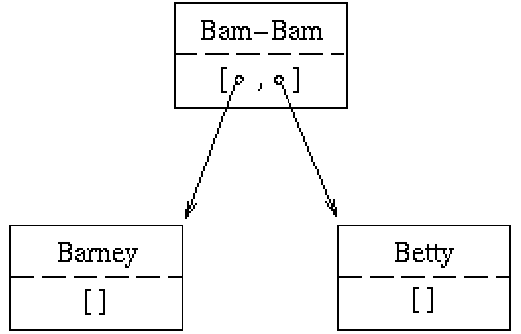
\includegraphics[width=3in,height=1.9in]{ub-img/ub-img6.png}
\end{center}

{\sffamily\bfseries Figure 2-1:}
{\sffamily A Record Containing a List of Two Records}

\bigskip

To find every node related to variable \texttt{bambam}, follow all the
links reachable starting from \texttt{bambam}. Here is a procedure that
performs this task.

\iconcode{
procedure print\_relatives(n) \\
local i \\
static relatives \\
initial relatives := set() \\
every i := n {\textbar} !n.links do \{  \\
\>   \ \ \ if not member(relatives, i.name) then \{  \\
\>   \ \ \ \ \ \ write(i.name) \\
\>   \ \ \ \ \ \ insert(relatives, i.name) \\
\>   \ \ \ \ \ \ print\_relatives(i) \\
\>   \ \ \ \ \ \ \} \\
\>   \ \ \ \} \\
end
}

Calling print\_relatives(bambam) will print

\iconcode{
Bam-Bam\\
Barney\\
Betty
}

Static variables and the \texttt{initial} clause are explained in
Chapter 1. Can you guess what purpose \index{static}static variable
\texttt{relatives} serves? For a proper tree structure, it is not
needed at all, but for more general data structures such as directed
graphs this static variable is very important! One defect of this
procedure is that there is no way to reset the static variable and call
\texttt{print\_relatives()} starting from scratch. How would you remove
this defect?

\subsection{The $n$-Queens Example}

The \index{8-Queens problem}8-Queens problem is a classic
\index{backtracking}backtracking problem. The goal is to place eight
queens on a chessboard so that none of the queens attack any other.
Here is a solution to a more general form of the problem, that of
placing \index{n queens}\textit{n} queens on an \textit{n} \texttt{x}
\textit{n} board. The solution we present is by Steve \index{Wampler,
Steve}Wampler, and it is in the Icon Program Library.

An array of size \texttt{n} stores the solutions, with each element
representing a column. The values in the array are integers specifying
the row in each column that has the queen. (Since the queens cannot
attack each other, each column must contain exactly one queen.) The
problem size \texttt{n} and the array are declared \texttt{global} so
that all procedures can see them; this allows the program to avoid
passing these variables in to every procedure call. Use globals
sparingly, and only where they are appropriate, as is the case here.

\iconcode{
link options \\
global solution, n \\
procedure main(args) \\
local i, opts
}

The program starts by handling command-line arguments. In Unicon
programs, \texttt{main()} is called with a single parameter that is a
list of strings whose elements are the command-line arguments of the
program.

The n-queens program recognizes only one thing on the command line: the
option \texttt{{}-n} followed by an integer specifies the size of board
to use. Thus the command line \texttt{queens -n 9} will generate
solutions on a 9x9 board. The default value of \texttt{n} is 6. The
\index{options()}\texttt{options()} procedure is an Icon Program
Library procedure described in Appendix B; it removes options from the
command line and places them in a table whose keys are option letters
such as \texttt{"n"}. Library procedures
such as \texttt{options()} are incorporated into a program using the
\index{link}\texttt{link} declaration, as in the \texttt{link options}
that begins the code fragment above. A link declaration adds the
procedures, global variables, and record types in the named module (in
this case, procedure \texttt{options()} came from a file
\texttt{options.icn}) to the program.

\iconcode{
\>   opts := options(args,"n+") \\
\>   n := {\textbackslash}opts["n"]
{\textbar} 6 \\
\>   if n {\textless}= 0 then stop("-n needs a positive
numeric parameter")
}

The value \texttt{n} gives the size for the solution array and also
appears in a banner:

\iconcode{
\>   solution := list(n) \ \ \# a list of column solutions \\
\>   write(n,"-Queens:") \\
\>   every q(1) \ \ \ \ \ \ \ \ \ \ \ \# start by placing queen in
first column \\
end
}

Now comes the meat of the program, the procedure \texttt{q(c)}. It tries
to place a queen in column \texttt{c} and then calls itself recursively
to place queens in the column to the right. The \texttt{q(c)} procedure
uses three arrays: \texttt{rows}, \texttt{up}, \ and \texttt{down}.
They are declared to be \textit{static}, meaning that their values will
be preserved between executions of the procedure, and all
\index{instance}instances of the procedure will share the same lists.
Since each row must have exactly one queen, the rows array helps to
make sure any queen that is placed is not on a row that already has a
queen. The other two arrays handle the diagonals: \texttt{up} is an
array (of size \textit{2n-1}) of the upward slanting diagonals, and
\texttt{down} is an array for the downward slanting diagonals. Two
queens in positions \textit{(r\_1, c\_1)} and \textit{(r\_2, c\_2)} are
on the same "up" diagonal if
\textit{n+r\_1-c\_1 = n+r\_2-c\_2} and they are on the same
"down" diagonal if \textit{r\_1+c\_1-1 =
r\_2+c\_2-1}. Figure 2-2 shows some of the
``up'' and ``down'' diagonals.

\bigskip

\begin{center}
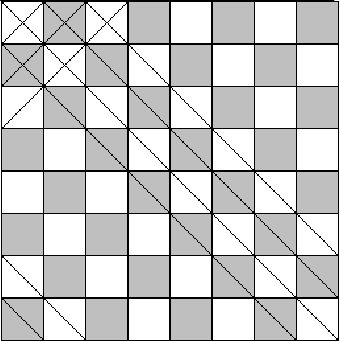
\includegraphics[width=3.5in,height=3.5in]{ub-img/diagonal.png}
\end{center}
{\sffamily\bfseries Figure 2-2:}
{\sffamily Up and Down Diagonals in the n-Queens Problem}

\bigskip

\iconcode{
\# \\
\# q(c) - place a queen in column c. \\
\# \\
procedure q(c) \\
local r \\
static up, down, rows \\
initial \{ \\
\>   up := list(2*n-1,0) \\
\>   down := list(2*n-1,0) \\
\>   rows := list(n,0) \\
\>   \}
}

The next expression in \texttt{q()} is an \texttt{every} loop that tries
all possible values for the queen in row \texttt{c}. The variable
\texttt{r} steps through rows 1 to 8. For any row at which the program
places a queen, it must ensure that

1.\ \ \texttt{rows[r]} is zero, that is, no other column has a queen in
row \texttt{r}\texttt{,}

2.\ \ \texttt{up[n+r-c]} is 0, that is, there is not already a queen in
the "up" diagonal, and

3.\ \ \texttt{down[r+c-1]} is 0, that is, there is not already a queen
in the down diagonal.

If these conditions are met, then it is OK to place a queen by assigning
a 1 to all those arrays in the appropriate position:

\iconcode{
\>   every 0 = rows[r := 1 to n] = up[n+r-c] = down[r+c-1] \& \\
\>   \ \ \ rows[r] {\textless}- up[n+r-c] {\textless}- down[r+c-1]
{\textless}- 1 do \{
}

For \index{assignment}assignment, instead of \texttt{:=} this expression
uses the \index{reversible assignment}\textit{reversible assignment}
operator \texttt{{\textless}-}. This assigns a value just like in
conventional assignment, but it remembers the old value; if it is ever
resumed, it restores the old value and \index{expression failure}fails.
This causes the appropriate entries in the \texttt{row},
\texttt{up}\texttt{,} and \texttt{down} arrays will be reinitialized
between iterations.

When the \texttt{every} loop found a good placement for this column,
either the program is done (if this was the last column) or else it is
time to try to place a queen in the next row:

\iconcode{
\>   \ \ \ solution[c] := r \ \ \ \ \ \ \# record placement. \\
\>   \ \ \ if c = n then show() \\
\>   \ \ \ else q(c + 1) \ \ \ \ \ \ \ \ \ \# try to place next queen. \\
\>   \ \ \ \} \\
end
}

That's it! The rest of the program just prints out any
solutions that were found.

Printing the chess board is similar to other reports you might write
that need to create horizontal lines for tables. The \texttt{repl()}
function is handy for such situations. The \texttt{repl(s, i)} function
returns \texttt{i} "replicas" of string
\texttt{s} concatenated together. The \texttt{show()} function uses it
to create the chessboard.\textit{ }

\iconcode{
\# \\
\# show the solution on a chess board. \\
\# \\
procedure show() \\
static count, line, border \\
initial \{ \\
\>   count := 0 \\
\>   line := repl("{\textbar} \ \ ",n)
{\textbar}{\textbar} "{\textbar}" \\
\>   border := repl("-{}-{}-{}-",n)
{\textbar}{\textbar} "-" \\
\>   \} \\
\>   write("solution: ", count+:=1,
"{\textbackslash}n \ ", border) \\
\>   every line[4*(!solution - 1) + 3] {\textless}-
"Q" do \{ \\
\>   \ \ \ write(" \ ", line,
{\textquotedblleft}{\textbackslash}n \ ", border) \\
\>   \ \ \ \} \\
\>   write() \\
end
}

\section{Summary}

Unicon's structures are better than sliced bread. To be fair, this is because
Icon's inventors really got things right. These structures are the foundations
of complex algorithms and the glue that builds sophisticated data models. They
are every computer scientists' buzzword-compliant best friends: polymorphic,
heterogeneous, implicitly referenced, cycle-capable, dynamically represented,
and automatically reclaimed.  They provide a direct implementation of the common
information associations used in object-oriented design. But most important of
all, they are extremely simple to learn and use.



% \clearpage
% \ \\ \bigskip

\chapter{String Processing}

In addition to its groundbreaking expression evaluation, Unicon inherits
other compelling features from Icon that reduce the effort required to
write complex programs. Icon's ancestor is
\index{SNOBOL4}SNOBOL4, the grandfather of all string processing
languages, and from it come some of the most flexible and readable
built-in string processing facilities found in any language. In this
chapter you will learn

\begin{itemize}
\item How to manipulate strings and sets of characters
\item Icon's string scanning \index{control
structure}control structure
\item How to write custom \index{pattern matching}pattern matching
primitives, with \index{backtracking}backtracking
\end{itemize}
Techniques for matching regular expressions and context free grammars

\section{String Indexes}

You have already seen string literals delimited by double quotes, and
the most common operators that work on strings: the size of a string is
given by the unary \texttt{*} operator, substrings can be picked out
with indexes, and two strings can be concatenated with the
\texttt{{\textbar}{\textbar}} operator. Now it is time to present a
deeper understanding of the meaning of indexes as they are used with
strings and lists.

\index{string!indexes 1 based}Indexes in a string refer to the positions
between characters. The positions are numbered starting from 1. The
index 0 refers to the position after the last character in the string,
and negative indices count from the right side of the string:


\begin{center}
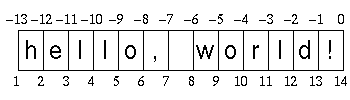
\includegraphics[width=3.6075in,height=1.0417in]{ub-img/ub-img7.png}
\end{center}
\vspace{-0.25cm}{\sffamily\bfseries Figure 3-1:}
{\sffamily Positive and Negative String Indices}

\bigskip

The expression \index{slice!string s[i:j]}\texttt{s[i:j]} refers to the
\index{substring}substring of \texttt{s} that lies between positions
\texttt{i} and \texttt{j}. If either \texttt{i} or j is not a valid
index into \texttt{s}, the expression fails. The expression
\texttt{s[k]} is short for \texttt{s[k:k+1]} and refers to a single
\index{character}character at position \texttt{k}. The expression
\texttt{s[k+:n]} is the substring of length \texttt{n} starting at
position \texttt{k}. If \texttt{s} is the string
\texttt{"hello, world!"} then the
expressions

\iconcode{
s[7] := " puny " \\
s[13:18] := "earthlings"
}

\noindent
change \texttt{s} into \texttt{"hello, puny
earthlings!"}, illustrating the ease with which
insertions and substitutions are made. The first assignment changes the
string to \texttt{"hello, puny world!"},
replacing a single character with six characters and thereby increasing
its length. The second assignment operates on the modified string,
replacing \texttt{"world"} with
\texttt{"earthlings"}.

Strings are values, just like numbers; if you copy a string and then
work on the copy, the original will be left unchanged:

\iconcode{
s := "string1" \\
new\_s := s \\
new\_s[7] := "2"
}

Now the value of \texttt{new\_s} is
"string2" but \texttt{s} is left unchanged.

As mentioned in Chapter 1, strings can be compared with string
\index{comparison operator!string}comparison operators such as
\texttt{==}.

\iconcode{
if line[1] == "\#" then ...}

If you find you are writing many such tests, the string processing you
are doing may be more cleanly handled using the string scanning
facilities, described below. But first, here is some more detail on the
character set data type, which is used in many of the string scanning
functions.

\section{Character Sets}

A cset is a set of characters. It has the usual properties of sets:
order is not significant, and a character can only occur once in a
cset. A \index{cset literal}cset literal is represented with single
quotes:

\iconcode{
c := 'aeiou'}

Since characters can only occur once in a cset, duplicates in a cset
literal are ignored; for example,
\texttt{'aaiiee'} is equivalent to
\texttt{'aie'}. Strings can be
converted to csets and vice versa. Since csets do not contain
duplicates, when a string is converted to a cset, all the duplicates
are removed.

Therefore to see if a string is composed of all the vowels and no
consonants:

\iconcode{
if cset(s) == 'aeiou' then ...}

Or, to find the number of distinct characters in a string:

\iconcode{
n := *cset(s)}

The \texttt{!} operator generates the members of a cset in sorted order;
this is also useful in some situations.

\section{Character Escapes}

Both strings and csets rely on the backslash as an escape character
within string literals. A backslash followed by an \index{escape
codes}\textit{escape code} of one or more characters specifies a
non-printable or control character. Escape codes may be specified by a
numeric value given in hex or octal format - for example,
\texttt{"{\textbackslash}x41"}.
Alternatively, any control character may be specified with an escape
code consisting of the caret (\texttt{\^{}}) followed by the alphabetic
letter of the control character. A cset containing control-C,
control-D, and control-Z could be specified as
\texttt{'{\textbackslash}\^{}c{\textbackslash}\^{}d{\textbackslash}\^{}z'}.
For the most common character escapes, a single-letter code is defined,
such as \texttt{"{\textbackslash}t"} for
the tab character, or
\texttt{"{\textbackslash}n"} for the
newline. For all other characters, the character following the
backslash is the character; this is how quotes or backslashes are
included in literals. The escape codes are summarized in Table 3-1.

\medskip
% \pagebreak

\begin{center}
{\sffamily\bfseries
Table 3-1

Escape Codes and Characters 
}
\end{center}

\begin{center}
\begin{supertabular}{|m{0.38in}|m{0.8in}|m{0.4in}|m{0.855in}|m{0.38in}|m{1.14in}|m{0.38in}|m{0.68in}|}
\hline
\sffamily\bfseries Code &
\sffamily\bfseries Character &
\sffamily\bfseries Code &
\sffamily\bfseries Character &
\sffamily\bfseries Code &
\sffamily\bfseries Character &
\sffamily\bfseries Code &
\sffamily\bfseries Character\\\hline
\ \ {\textbackslash}b &
backspace &
\ \ {\textbackslash}d &
delete &
\ \ {\textbackslash}e &
escape &
\ \ {\textbackslash}f &
form feed\\\hline
\ \ {\textbackslash}l &
line feed &
\ \ {\textbackslash}n &
newline &
\ \ {\textbackslash}r &
carriage return &
\ \ {\textbackslash}t &
tab\\\hline
\ \ {\textbackslash}v &
vertical tab &
\ {\textbackslash}' &
quote &
\ \ {\textbackslash}" &
double quote &
\ \ {\textbackslash}{\textbackslash} &
backslash\\\hline
\ {\textbackslash}\textit{ooo} &
octal &
{\textbackslash}x\textit{hh} &
hexadecimal  &
\ {\textbackslash}\^{}\textit{x} &
Control-\textit{x} &
~
 &
~
\\\hline
\end{supertabular}
\end{center}

\section{String Scanning}

Icon's string analysis facility is called
\index{string!scanning}\textit{string scanning}. A
\index{scanning!environment}scanning environment consists of a string
\index{subject string}\index{string!subject}\textit{subject} and an
integer \index{position,
string}\index{string!position}\textit{position} within the subject at
which scanning is to be performed. These values are held by the keyword
variables \texttt{\&subject} and \texttt{\&pos}. Scanning environments
are created by an expression of the form

\iconcode{
\textit{s} ? \textit{expr}}

The binary \texttt{?} operator sets the subject to its left argument and
initializes the position to 1; then it executes the expression on the
right side.

The expression usually has \index{matching functions}\textit{matching
functions} in it. Matching functions change the position, and return
the substring between the old and new positions. For example:
\texttt{move(j)}\texttt{ }moves the position \texttt{j} places to the
right and returns the substring between the old and new position. This
string will have exactly \texttt{j} characters in it. When the position
cannot move as directed, for example because there are less than
\texttt{j} characters to the right, \index{move(i)}\texttt{move()}
fails. Here is a simple example:

\iconcode{
text ? \{ \\
\>   while move(1) do \\
\>   \ \ \ write(move(1)) \\
\>   \}
}

This code writes out every other character of the string in variable
\texttt{text}.

Another function is \index{tab(i)}\texttt{tab(i)}, which sets the
position \texttt{\&pos} to its argument and returns the substring that
it passed over. So the expression \texttt{tab(0)} will return the
substring from the current position to the end of the string, and set
the position to the end of the string.

String scanning functions examine a string and generate the interesting
positions in it. We have already seen \index{find()}\texttt{find()},
which looks for substrings. In addition to the other parameters that
define what the function looks for, these string functions end with
three optional parameters: a string to examine and two integers. These
functions \index{default!scanning parameters}default their string
parameter to \texttt{\&subject}, the string being scanned. The two
integer positions specify where in the string the processing will be
performed; they default to 1 and 0 (the entire string), or
\texttt{\&pos} and 0 if the string defaulted to use \texttt{\&subject}.
Here is a \index{generator}generator that produces the words from the
input:

\iconcode{
procedure getword() \\
local wchar, line \\
\>   wchar := \&letters ++ \&digits ++
'{\textbackslash}'-' \\
\>   while line := read() do \\
\>   \ \ \ line ? while tab(upto(wchar)) do \{ \\
\>   \ \ \ \ \ \ word := tab(many(wchar)) \\
\>   \ \ \ \ \ \ suspend word \\
\>   \ \ \ \ \ \ \} \\
end
}

Variable \texttt{wchar}\texttt{ }is a cset of characters that are
allowed in words, including apostrophe (which is escaped) and hyphen
characters. \index{upto(c)}\texttt{upto(c)} returns the next position
at which a character from the cset \texttt{c} occurs. The
\index{many(c)}\texttt{many(c)} function returns the position after a
sequence of characters from \texttt{c}, if one or more of them occur at
the current position. The expression \texttt{tab(upto(wchar))} advances
the position to a character from \texttt{wchar}; then
\texttt{tab(many(wchar))} moves the position to the end of the word and
returns the word that is found. This is a generator, so when it is
resumed, it takes up execution from where it left off and continues to
look for words (reading the input as necessary).

Notice the first line: the cset \texttt{wchar} is the set union of the
upper- and lowercase letters (the value of the keyword
\texttt{\&letters}) and the digits (the keyword \texttt{\&digits}).
This cset union is performed each time \texttt{getword()} is called,
which is inefficient. Instead, the procedure ought to calculate the
value and store it for all future calls to \texttt{getword()}.

To do this, you declare the variable to be static, causing its value to
persist across calls to the procedure. Normal local variables are
initialized to the null value each time a procedure is entered. To do
this, add these two lines to the beginning of the procedure:

\iconcode{
static wchar \\
initial wchar := \&letters ++ \&digits ++
'{\textbackslash}'-'
}

The \index{match(s)}\texttt{match(s)} function takes a string argument
and succeeds if \texttt{s} is found at the current position in the
subject. If it succeeds, it produces the position at the end of the
matched substring. This expression

\iconcode{
if tab(match("-")) then sign := -1 else sign
:= 1}

\noindent
looks to see if there is a minus sign at the current position; if one is
found, \texttt{\&pos} is moved past it and the variable \texttt{sign}
is assigned a -1; otherwise, it gets a 1. The expression
\texttt{tab(match(s))} occurs quite often in string scanning, so it is
given a shortcut: \texttt{=s} does the same thing.

The last two string scanning functions to round out
Icon's built-in repertoire are
\index{any(c)}\texttt{any(c)} and \index{bal()}\texttt{bal(c1,c2,c3)}.
\texttt{any(c)} is similar to \texttt{many()}, but only tests a single
character being scanned to see if it is in cset \texttt{c}. The
\texttt{bal()} function produces positions at which a character in
\texttt{c1} occurs, similar to \texttt{upto()}, with the added
stipulation that the string up to those positions is \textit{balanced}
with respect to characters in \texttt{c2} and \texttt{c3}. A string is
balanced if it has the same number of characters from \texttt{c2} as
from \texttt{c3} and there are at no point more \texttt{c3} characters
present than \texttt{c2} characters. The \texttt{c1} argument defaults
to \texttt{\&cset}. Since \texttt{c2} and \texttt{c3} default to
\texttt{'('} and
\texttt{')'}, \texttt{bal()} defaults
to find balanced parentheses.

The restriction that \texttt{bal()} only returns positions at which a
character in \texttt{c1} occurs is a bit strange. Consider what you
would need to do in order to write an expression that tells whether a
string \texttt{s} is balanced or not.

You might want to write it as \texttt{s ? (bal() = *s+1)} but
\texttt{bal()} will never return that position. Concatenating an extra
character solves this problem:

\iconcode{
procedure isbalanced(s) \\
\>   return (s {\textbar}{\textbar} " ") ?
(bal() = *s+1) \\
end
}

If string \texttt{s} is very large, this solution is not cheap, since it
creates a new copy of string \texttt{s}. You might write a version of
\texttt{isbalanced()} that doesn't use the
\texttt{bal()} function, and see if you can make it run faster than
this version. An example later in this chapter shows how to use
\texttt{bal()} in a more elegant manner.

\subsection*{File Completion}

Consider the following gem, attributed to Jerry \index{Nowlin,
Jerry}Nowlin and Bob \index{Alexander, Bob}Alexander. Suppose you want
to obtain the full name of a file, given only the first few letters of
a filename and a list of complete \index{filename completion}filenames.
The following one line procedure does the trick:

\iconcode{
procedure complete(prefix, filenames) \\
\>   suspend match(prefix, p := !filenames) \& p \\
end
}

This procedure works fine for lists with just a few members and also for
cases where \texttt{prefix} is fairly large.

\subsection*{Backtracking}

\index{backtracking}The matching functions we have seen so far,
(\texttt{tab()} and \texttt{move()}), are actually
\index{generator}generators. That is, even though they only produce one
value, they suspend instead of returning. If expression evaluation ever
resumes one of these functions, they restore the old value of
\texttt{\&pos}. This makes it easy to try alternative matches starting
from the same position in the string:

\iconcode{
s ? (="0x" \& tab(many(\&digits ++
'abcdefABCDEF'))) {\textbar} \\
\>   tab(many(\&digits))
}

This expression will match either a hexadecimal string in the format
used by C or a decimal integer. Suppose \texttt{s} contains the string
\texttt{"0xy"}. The first part of the
expression succeeds and matches the
\texttt{"0x"}; but then the expression
\texttt{tab(many(\&digits ++
'abcdef'))} fails; this causes Unicon
to resume the first \texttt{tab()}, which resets the position to the
beginning of the string and fails. Unicon then evaluates the expression
\texttt{tab(many(\&digits))} which succeeds (matching the string
\texttt{"0"}); therefore the entire
expression succeeds and leaves \texttt{\&pos} at 2.

{\sffamily\bfseries
Warning}

{\sffamily
Be careful when using tab() or move() in a surrounding expression that
can fail! The fact that tab() and move() reset \&pos upon expression
failure causes confusion and bugs when it happens accidentally.}

\subsection*{Concordance Example}

Listing 3-1 illustrates the above concepts and introduces a few more.
Here is a program to read a file, and generate a
\index{concordance}concordance that prints each word followed by a list
of the lines on which it occurs. Short words like
\texttt{"the"} aren't
interesting, so the program only counts words longer than three
characters. 

\bigskip

{\sffamily\bfseries Listing 3-1}
{\sffamily\bfseries A simple concordance program}

\iconcode{
procedure main(args) \\
\>   (*args = 1) {\textbar} stop("Need a
file!") \\
\>   f := open(args[1]) {\textbar}
stop("Couldn't open ",
args[1]) \\
\>   wordlist := table() \\
\>   lineno := 0 \\
\ \\
\>   while line := map(read(f)) do \{ \\
\>   \ \ \ lineno +:= 1 \\
\>   \ \ \ every word := getword(line) do  \\
\>   \ \ \ \ \ \ if *word {\textgreater} 3 then \{ \\
\>   \ \ \ \ \ \ \ \ \ \# if word isn't in the table, 
	set entry to empty list \\
\>   \ \ \ \ \ \ \ \ \ /wordlist[word] := list() \\
\>   \ \ \ \ \ \ \ \ \ put(wordlist[word], lineno) \\
\>   \ \ \ \ \ \ \ \ \ \} \\
\>   \ \ \ \} \\
\>   L := sort(wordlist) \\
\>   every l := !L do \{ \\
\>   \ \ \ writes(l[1],
"{\textbackslash}t") \\
\>   \ \ \ linelist := "" \\
\>   \ \ \ \# Collect line numbers into a string \\
\>   \ \ \ every linelist {\textbar}{\textbar}:= (!l[2]
{\textbar}{\textbar} ", ") \\
\>   \ \ \ \# trim the final ", " \\
\>   \ \ \ write(linelist[1:-2]) \\
\>   \ \ \ \} \\
end \\
\ \\
procedure getword(s) \\
\>   s ? while tab(upto(\&letters)) do \{ \\
\>   \ \ \ word := tab(many(\&letters)) \\
\>   \ \ \ suspend word \\
\>   \ \ \ \} \\
end
}

\noindent If we run this program on this input: 

\iconcode{
Half a league, half a league, \\
Half a league onward, \\
All in the valley of Death \\
Rode the six hundred.
}

\noindent the program writes this output: 

\iconcode{
death \ \ 3 \\
half \ \ \ 1, 2 \\
hundred 4 \\
league \ 1, 1, 2 \\
onward \ 2 \\
rode \ \ \ 4 \\
valley \ 3
}

First, note that the \texttt{main()} procedure requires a command-line
argument, the name of a file to open. Also, we pass all the lines read
through the function \texttt{map()}. This is a function that takes
three arguments, the first being the string to map; and the second and
third specifying how the string should be mapped on a character by
character basis. The defaults for the second and third arguments are
the uppercase letters and the lowercase letters, respectively;
therefore, the call to \texttt{map()} converts the line just read in to
all \index{lower case}lowercase.

\section{Regular Expressions}

The Icon Program Library (included with the Unicon distribution)
provides \index{regular expression}regular expression matching
functions. To use it, add the line \texttt{link regexp} at the top of
the program. Listing 3-2 is an example of a search-and-replace program
called (somewhat inappropriately)
\texttt{i}\index{grep}\texttt{grep}\texttt{.icn}: The actual searching
and replacing is performed on each line of text by procedure
\texttt{re\_sub()}. This procedure illustrates many classic aspects of
string scanning. It marches through the string from right to left using
a while loop. It builds up a result string, which by default would be a
copy of its scanned string. At the start of each occurrence of the
regular expression, the replacement string is appended to the result,
and the regular expression is tabbed over and not appended to the
result. When no more occurrences of the regular expression are found,
the remainder of the string is appended to the result.

\bigskip

{\sffamily\bfseries Listing 3-2}
{\sffamily\bfseries A simple grep-like program}

\iconcode{
link regexp \\
procedure main(av) \\
\>   local f, re, repl \\
\>   every (f{\textbar}re{\textbar}repl) := pop(av) \\
\>   f := open(f) {\textbar} stop("can't open file named: ", f) \\
\>   while line := read(f) do \\
\>   \ \ \ write(re\_sub(line, re, repl)) \\
end \\
procedure re\_sub(str, re, repl) \\
\>   result := "" \\
\>   str ? \{ \\
\>   \ \ \ while j := ReFind(re) do \{ \\
\>   \ \ \ \ \ \ result {\textbar}{\textbar}:= tab(j)
{\textbar}{\textbar} repl \\
\>   \ \ \ \ \ \ tab(ReMatch(re)) \\
\>   \ \ \ \ \ \ \} \\
\>   \ \ \ result {\textbar}{\textbar}:= tab(0) \\
\>   \ \ \ \} \\
\>   return result \\
end
}

To replace all occurrences of
"read{\textbar}write" with
"IO operation" you could type 

\iconcode{
igrep mypaper.txt "read{\textbar}write"
"IO Operation"}

Since the program has access to the pattern matching operation at a
finer grain, more complex operations are possible, this
search-and-replace is just an example.

\section{Grammars}

\index{grammar}Grammars are collections of rules that describe
\index{syntax}\textit{syntax}, the combinations of words allowed in a
language. Grammars are used heavily both in linguistics and in computer
science. \index{pattern matching}Pattern matching using a grammar is
often called \index{parse}\textit{parsing}, and is one way to match
patterns more complex than regular expressions can handle. This section
presents some simple programming techniques for parsing context free
grammars. Context free grammars utilize a \index{stack}stack to
recognize a fundamentally more complex category of patterns than
regular expressions can; they are defined below.

For linguists, this treatment is elementary, but introduces useful
programming techniques. For writers of programming language compilers,
an automatic parser generator tool that you can use with Unicon or Icon
is described in Chapter 18. If you are not interested in grammars, you
can skip the rest of this chapter.

A \index{context-free grammar}context-free grammar or CFG is a set of
rules or \textit{productions}. Here is an example:

\iconcode{
S -{\textgreater} S S \\
\>   {\textbar} ( S ) \\
\>   {\textbar} ( )
}

This grammar has three productions. There are two kinds of symbols,
\textit{non-terminals} like \texttt{S} that can be replaced by the
string on the right side of a rule, and \textit{terminals} like
\texttt{(} and \texttt{)}. An application of a production rule is called
a derivation. One special non-terminal is called the
\textit{start symbol}; a string is accepted by the grammar if there is a
sequence of derivations from the start symbol that leads to the string.
By convention the start symbol is the first non-terminal in the
definition of the grammar. (This grammar only has one non-terminal, and
it is also the start symbol.)

This grammar matches all strings of balanced parentheses. The string
\texttt{(()(()()))} can be matched by this derivation:

\iconcode{
S -{\textgreater} (S) -{\textgreater} (SS) -{\textgreater} (()S)
-{\textgreater} (()(S)) -{\textgreater} \\
\>   \ \ (()(SS)) -{\textgreater} (()(()S)) -{\textgreater} (()(()()))
}

\subsection*{Parsing}

Unicon can parse grammars in a natural way using matching
functions. A production

\iconcode{
A -{\textgreater} B a D  \\
\>   {\textbar} C E b
}

\noindent
can be mapped to this matching function:

\iconcode{
procedure A() \\
\>   suspend (B() \& ="a" \& D())
{\textbar} (C() \& E() \& ="b") \\
end
}

\noindent
This procedure first tries to match a string matched by \texttt{B},
followed the character \texttt{a}, followed by a string matched by
\texttt{D}. If \texttt{D} \index{expression failure}fails, execution
backtracks across the \texttt{="a"}
(resetting \texttt{\&pos}) and resume \texttt{B()}, which will attempt
the next match.

If the sub-expression to the left of the \index{alternation operator (
{\textbar} )}alternation fails, then execution will try the
sub-expression on the right, \texttt{C() \& E() \&
="b"} until something matches - in which
case \texttt{A} succeeds, or nothing matches - which will cause it to
fail.

Parsers for any CFG can be written in this way. However, this is an
expensive way to do it! Unicon's
expression evaluation will try all possible derivations
trying to match a string. This is not a good way to parse, especially
if the grammar is amenable to lookahead methods. A more efficient
method is given in the next section. For serious parsing jobs, Chapter
18 shows how to use the Unicon versions of the standard
industrial-strength lexical analyzer and parser generation tools, lex
and yacc.

\subsection*{Doing It Better}

Many grammars can be parsed more efficiently using
well-known techniques - consult a book on compilers for details. Here
is one way of parsing a grammar using some of the built-in
functions. Consider this grammar for an arithmetic expression:

\iconcode{
E -{\textgreater} T {\textbar} T + E \\
T -{\textgreater} F {\textbar} F * T \\
F -{\textgreater} a {\textbar} b {\textbar} c {\textbar} ( E )
}

\noindent
Listing 3-3 is an Unicon program that recognizes strings produced by
this grammar:

\bigskip

{\sffamily\bfseries Listing 3-3}
{\sffamily\bfseries Expression parser}

\iconcode{
procedure main() \\
\>   while line := read() do \\
\>   \ \ \ if expr(line) == line then write("Success!") \\
\>   \ \ \ else write("Failure.") \\
end \\
procedure expr(s) \\
\>   s ? \{ \\
\>   \ \ \ while t := tab(bal('+'))
do \{ \\
\>   \ \ \ \ \ \ term(t) {\textbar} \index{fail}fail ;
="+" \\
\>   \ \ \ \ \ \ \} \\
\>   \ \ \ term(tab(0)) {\textbar} fail \\
\>   \ \ \ \} \\
\>   return s \\
end \\
procedure term(s) \\
\>   s ? \{ \\
\>   \ \ \ while f := tab(bal('*'))
do \{ \\
\>   \ \ \ \ \ \ factor(f) {\textbar} fail ;
="*" \\
\>   \ \ \ \ \ \ \} \\
\>   \ \ \ factor(tab(0)) {\textbar} fail \\
\>   \ \ \ \} \\
\>   return s \\
end \\
procedure factor(s) \\
\>   s ? suspend ="a" {\textbar}
="b" {\textbar}
="c" {\textbar}  ( ="("
{\textbar}{\textbar}
expr(tab(bal(')')))
{\textbar}{\textbar} =")" ) \\
end
}

The interesting procedure here is \index{bal()}\texttt{bal()}. With
\texttt{')'} as its first argument,
\texttt{bal()} scans to the closing parenthesis, skipping over any
parentheses in nested subexpressions, which is exactly what is needed
here.

The procedure \texttt{factor()} is written according to the rule in the
previous section. The procedures \texttt{expr()} and \texttt{term()}
have the same structure. The \texttt{expr()} procedure skips any
subexpressions (with balanced parentheses) and looks for a \texttt{+}.
We know that this substring is a well-formed expression that is not a
sum of terms, therefore, it must be a term. Similarly \texttt{term()}
looks for \texttt{*} and it knows that the expression does not contain
any \texttt{*} operators at the same nesting level; therefore it must
be a factor.

Notice that the procedures return the strings that they matched. This
allows us to check if the whole line matched the grammar rather than
just an initial substring. Also, notice that \texttt{factor()} uses
string concatenation instead of conjunction, so that it can return the
matched substring.

\section*{Summary}

Unicon's string processing facilities are extensive.
Simple operations are very easy, while more complex string analysis has
the support of a special control structure, string scanning. String
scanning is not as concise as regular expression pattern matching, but
it is fundamentally more general because the code and patterns are
freely intermixed.



\clearpage\section{Chapter 4: Advanced Language Features}

The previous chapters described a wide range of built-in computational
facilities that comprise much of what makes Unicon a great language.
This chapter delves into interesting features that help make Unicon
more than just the sum of its parts. This chapter demonstrates the
following tasks:

\begin{itemize}
\item Controlling expressions more precisely
\item Using list structures and procedure parameter lists
interchangeably
\item Holding a \index{generator}generator expression in a value so that
its results can be used in different locations throughout the program
\item Defining your own \index{control structure}control structures
\item Evaluating several generator expressions in parallel
\item Permuting strings using sophisticated mappings
\end{itemize}
\subsection[Limiting or Negating an Expression]{Limiting or Negating an
Expression}
\index{limiting an expression}Chapter 1 described generators and the
expression mechanism without mentioning many methods for using them,
other than \textsf{every} loops. Suppose you wish to generate five
elements from a table. If the table has thousands of elements, then you
may want to generate just five elements precisely in a situation where
generating all the table elements with \textsf{!T} is infeasible. You
could write an \textsf{every} loop that breaks out after five
iterations, but this solution isn{\textquotesingle}t easy to use within
some more complex expressions. The binary backslash operator
\textsf{\textit{expr}}\textsf{ {\textbackslash} }\textsf{\textit{i}}
limits \textsf{\textit{expr}} to at most \textsf{\textit{i}} results.
If \textsf{expr} has fewer results, the limitation operator has no
effect; once \textsf{\textit{i}} results have been obtained, limitation
causes the expression to \index{expression failure}fail even if it
could produce more results.

Unicon does not have a boolean type, so it might not have surprised you
that Chapter 1 downplayed the standard logical operators. The
\index{alternation operator ( {\textbar} )}alternation operator
(\textsf{{\textbar}}) resembles a short-circuit \index{OR operator}OR
operator, since it generates its left operand and only evaluates its
right operand if the left operand or the surrounding expression fails.
The conjunction operator (\textsf{\&}) resembles a short-circuit
\index{AND operator}AND operator, since it evaluates its left operand,
and if that operand succeeds, then the result of the conjunction is the
result of its right operand. The reserved word \textsf{not} rounds out
the boolean-like operators. If \textsf{\textit{expr}} produces no
results, then \index{not}\textsf{not }\textsf{\textit{expr}} will
succeed (and produce a null value); if \textsf{\textit{expr}} produces
any results, then the \textsf{not} expression fails. The \textsf{not}
operator can remedy certain forms of generator confusion. Compare the
following two expressions:

\iconcode{
if not (s ==
({\textquotedbl}good{\textquotedbl}{\textbar}{\textquotedbl}will{\textquotedbl}{\textbar}{\textquotedbl}hunting{\textquotedbl}))
then write({\textquotedbl}nope{\textquotedbl})}

\iconcode{
if (s \~{}==
({\textquotedbl}good{\textquotedbl}{\textbar}{\textquotedbl}will{\textquotedbl}{\textbar}{\textquotedbl}hunting{\textquotedbl}))
then write({\textquotedbl}uh huh{\textquotedbl})}

The first expression uses \textsf{not} to ensure that string \textsf{s}
is none of the three words. The second expression always writes
\textsf{{\textquotedbl}uh huh{\textquotedbl}}, because any string
\textsf{s} that you pick will be not equal (\textsf{\~{}==}) to at
least one of the three strings in the alternation. The \textsf{then}
part will always execute, which is probably not what was intended.

{\sffamily\bfseries
Note}

{\sffamily
Negating an == operator is not the same as using a \~{}== operator. You
have been warned!}

The \index{conjunction \&}conjunction operator
\textsf{\textit{expr}}\textsf{\textit{\textsubscript{1}}}\textsf{ \&
}\textsf{\textit{expr}}\textsf{\textit{\textsubscript{2}}} has an
alternate syntax, a comma-separated list of expressions in parentheses:
\textsf{(}\textsf{\textit{expr}}\textsf{\textit{\textsubscript{1}}}\textsf{
, }\textsf{\textit{expr}}\textsf{\textit{\textsubscript{2}}}\textsf{)}.
Any number of expressions may be present, and the whole expression only
succeeds if they all succeed. This looks similar to the syntax for a
procedure call because it is similar: a procedure call mutually
evaluates all the actual parameters before the procedure is invoked.
Besides putting a procedure value in front of a parenthesized argument
list, you can put a string or an integer. For a string value, as in
\textsf{s(x)}, a procedure by the name given in \textsf{s} is called;
if \textsf{s} had the value \textsf{{\textquotedbl}foo{\textquotedbl}},
then \textsf{s(x)} is the same as \textsf{foo(x)}. For an integer value
\textsf{i}, after all arguments are evaluated, the value of the entire
expression is the value of the \textsf{i}{\textquotesingle}th argument.

\subsection{List Structures and Parameter Lists}

The functions \textsf{write()} and \textsf{put()} take any number of
arguments; this flexibility helps make them powerful and convenient.
You can write \index{variable!no. of arguments}variable argument
procedures of your own by ending the last parameter in your procedure
declaration with empty square brackets:

\iconcode{
procedure myfunc(x, y, z[])}

In this case, instead of throwing away all arguments after the third,
the third parameter and all parameters that follow are placed into a
newly-constructed list. If you called the above procedure with
\textsf{myfunc(1, 2, 3, 4, 5)}, then \textsf{z} would have the value
\textsf{[3, 4, 5]}.

It is also useful to go the other direction and construct a list data
structure of dynamic (or user-supplied) length, and then call a
procedure with that list as its parameter list. The
\index{list!invocation}\index{apply operator}apply operator, binary
\textsf{!} performs this feat. If you call \textsf{write ! L}, then all
the elements of \textsf{L} are written contiguously on a single line
(unless they contain newline characters).

\subsection{Co-expressions}

A \index{co-expression}co-expression is an independent, encapsulated
\index{thread}thread{}-like context, where the results of an expression
(hopefully a generator!) can be picked off one at a time. Let us
consider an example. Suppose you are writing a program that generates
code, and you need something that will generate unique variable names.
This expression will generate names:

\iconcode{
{\textquotedbl}name{\textquotedbl} {\textbar}{\textbar} seq()}

The \index{seq()}\textsf{seq()} function produces an infinite sequence
of integers, by default starting at 1, so the whole expression
generates the sequence \textsf{{\textquotedbl}name1{\textquotedbl}},
\textsf{{\textquotedbl}name2{\textquotedbl}},
\textsf{{\textquotedbl}name3{\textquotedbl}}, ... and so forth. You can
put this expression at some point in your code; but you may need to use
it from several different places.

There are times when you need to separate the evaluation of an
expression from its textual position in the program. The normal
mechanism to do this would be a procedure. You can make separate calls
to a procedure from different locations in your program, but there is
no easy way to use the results from a single \index{instance}instance
of a generator in multiple locations. You can put all the results in a
list (not a good idea for generators with infinite result sequences) or
rewrite the procedure to produce the sequence using separate calls, but
this requires static or global variables, and is awkward at best. Here
is a crude effort

\iconcode{
procedure nameseq() \\
static i \\
initial i := 0 \\
\>   return {\textquotedbl}name{\textquotedbl} {\textbar}{\textbar} (i
+:= 1) \\
end
}

Now, consider the code generating program again. It may need not one
name sequence, but two kinds of names: statement labels and
temporary variables. It would be poor engineering to write a different
procedure for each such sequence. The \textsf{nameseq()}
procedure was already cumbersome for so simple a task, but generalizing
it for multiple kinds of names makes it \textit{really} messy. By
creating a pair of co-expressions, you can capture exactly what is
needed with a lot less code:

\iconcode{
labelname := create ({\textquotedbl}\_L{\textquotedbl}
{\textbar}{\textbar} seq()) \\
varname := create({\textquotedbl}\_V{\textquotedbl} {\textbar}{\textbar}
seq())
}

In both cases, \index{create}\textsf{create}\textsf{
}\textsf{\textit{expr}} allocates and initializes an evaluation context
plus the memory needed to evaluate expression \textit{expr}, but does
not start to evaluate it. Since the co-expression value may be used
outside the procedure call where it is created, the evaluation context
has to include a copy of the local variables and parameters used in the
expression. When a co-expression is \textit{activated}, it produces the
next value. A co-expression is activated by the @ operator. Each
activation of \textsf{labelname} will produce the next string in the
sequence \textsf{{\textquotedbl}\_L0{\textquotedbl}},
\textsf{{\textquotedbl}\_L1{\textquotedbl}},
\textsf{{\textquotedbl}\_L2{\textquotedbl}}, and so on. Similarly, each
activation \textsf{@varname}\textsf{ }produces the next in the sequence
\textsf{{\textquotedbl}\_V0{\textquotedbl}},
\textsf{{\textquotedbl}\_V1{\textquotedbl}},
\textsf{{\textquotedbl}\_V2{\textquotedbl}}, and so on. 

\iconcode{
loop\_name := @labelname \\
tempvar\_name := @varname
}

After a co-expression has produced all its results, further evaluation
with \textsf{@} will \index{fail!co-expression}fail. The \textsf{\^{}}
operator produces a new co-expression with the same expression as its
argument, but {\textquotedbl}rewound{\textquotedbl} to the beginning.

\iconcode{
\>   c := \^{}c}

\subsection[User{}-Defined Control Structures]{User-Defined Control
Structures}
\index{control structure}Control structures are those elements of a
language that determine in what order, and how many times, expressions
are executed. Co-expressions can be used to implement new
\textit{control structures} in the sense that procedures that take
co-expression arguments as parameters can control the order and number
of times their arguments are activated.

Consider a control structure that selects values from the first
expression at the positions specified by the second. This could be
invoked as:

\iconcode{
seqsel([create fibonacci(), create primes()])}

Assuming that you have a pair of \index{generator}generator procedures
that produce the Fibonacci numbers (1, 1, 2, 3, 5, 8, 13, \ ?) and the
primes (2, 3, 5, 7, 11, ?), this expression produces the numbers 1, 2,
5, 13, 89, .... Here is the implementation of \textsf{seqsel()}:

\iconcode{
procedure seqsel(a) \\
\>   (*a = 2) {\textbar} stop({\textquotedbl}seqsel requires a list of
two arguments{\textquotedbl}) \ \ \ \# We need two arguments \\
\>   e1 := a[1]; e2 := a[2] \\
\ \ \ \# position in the first stream we are looking at \\
\>   index := 1 \\
\>   repeat \{ \\
\>   \ \ \ \# Get the next index \\
\>   \ \ \ (i := @e2 ) {\textbar} fail \\
\ \ \ \ \ \ \# Keep getting values from the second expression until \\
\ \ \ \ \ \ \# we get to the i{\textquotesingle}th one. If e1 cannot produce that \\
\ \ \ \ \ \ \# many values, we fail. \\
\>   \ \ \ every index to i do \\
\>   \ \ \ (value := @e1) {\textbar} fail \\
\>   \ \ \ suspend value \\
\>   \ \ \ index := i+1 \\
\>   \ \ \ \} \\
end
}

Unicon provides a syntactic short-cut for this kind of usage:

\iconcode{
proc([create e1, create e2, ..., create en])
}

\noindent
can also be written with curly brackets, as

\iconcode{
proc\{e1, e2, ..., en\}
}

\subsection[Parallel Evaluation]{Parallel Evaluation}

\index{parallel evaluation}Co-expressions can be used to evaluate
expressions {\textquotedbl}in parallel{\textquotedbl} or in lock-step.
This program writes a table of \index{ASCII}ASCII characters with the
hex, decimal, and octal equivalents:

\iconcode{
procedure main() \\
\>   dec := create(0 to 255) \\
\>   hex\_dig := {\textquotedbl}0123456789abcdef{\textquotedbl} \\
\>   hex := create(!hex\_dig {\textbar}{\textbar} !hex\_dig) \\
\>   oct := create((0 to 3) {\textbar}{\textbar} (0 to 7)
{\textbar}{\textbar} (0 to 7)) \\
\>   char := create image(!\&cset) \\
\>   while write(@dec, {\textquotedbl}{\textbackslash}t{\textquotedbl},
@oct, {\textquotedbl}{\textbackslash}t{\textquotedbl}, @hex,
{\textquotedbl}{\textbackslash}t{\textquotedbl}, @char) \\
end
}

Co-expression \textsf{dec} produces the sequence 0, 1, 2, ... 255;
\textsf{hex} the sequence \textsf{{\textquotedbl}00{\textquotedbl}},
\textsf{{\textquotedbl}01{\textquotedbl}},
\textsf{{\textquotedbl}03{\textquotedbl}}, ...
\textsf{{\textquotedbl}ff{\textquotedbl}}; \textsf{oct}\textsf{ }the
sequence \textsf{{\textquotedbl}001{\textquotedbl}},
\textsf{{\textquotedbl}002{\textquotedbl}}, ...
\textsf{{\textquotedbl}377{\textquotedbl}}; and \textsf{char}\textsf{
}the sequence ..., \textsf{{\textquotedbl} {\textquotedbl}},
\textsf{{\textquotedbl}!{\textquotedbl}}, ...,
\textsf{{\textquotedbl}A{\textquotedbl}}, ...
\textsf{{\textquotedbl}Z{\textquotedbl}}, ...,
\textsf{{\textquotedbl}a{\textquotedbl}}, ...
\textsf{{\textquotedbl}z{\textquotedbl}}, and so forth.

Every invocation of \textsf{write()} results in all the co-expressions
being activated once, so they are all run in lock-step, producing this
table:

{\sffamily
0 \ \ \ \ \ \ 000 \ \ \ \ 00
\ \ \ \ \ {\textquotedbl}{\textbackslash}x00{\textquotedbl}}

{\sffamily
1 \ \ \ \ \ \ 001 \ \ \ \ 01
\ \ \ \ \ {\textquotedbl}{\textbackslash}x01{\textquotedbl}}

{\sffamily
2 \ \ \ \ \ \ 002 \ \ \ \ 02
\ \ \ \ \ {\textquotedbl}{\textbackslash}x02{\textquotedbl}}

{\sffamily
...}

{\sffamily
45 \ \ \ \ \ 055 \ \ \ \ 2d \ \ \ \ \ {\textquotedbl}-{\textquotedbl}}

{\sffamily
46 \ \ \ \ \ 056 \ \ \ \ 2e \ \ \ \ \ {\textquotedbl}.{\textquotedbl}}

{\sffamily
47 \ \ \ \ \ 057 \ \ \ \ 2f \ \ \ \ \ {\textquotedbl}/{\textquotedbl}}

{\sffamily
48 \ \ \ \ \ 060 \ \ \ \ 30 \ \ \ \ \ {\textquotedbl}0{\textquotedbl}}

{\sffamily
49 \ \ \ \ \ 061 \ \ \ \ 31 \ \ \ \ \ {\textquotedbl}1{\textquotedbl}}

{\sffamily
50 \ \ \ \ \ 062 \ \ \ \ 32 \ \ \ \ \ {\textquotedbl}2{\textquotedbl}}

{\sffamily
...}

{\sffamily
90 \ \ \ \ \ 132 \ \ \ \ 5a \ \ \ \ \ {\textquotedbl}Z{\textquotedbl}}

{\sffamily
91 \ \ \ \ \ 133 \ \ \ \ 5b \ \ \ \ \ {\textquotedbl}[{\textquotedbl}}

{\sffamily
92 \ \ \ \ \ 134 \ \ \ \ 5c
\ \ \ \ \ {\textquotedbl}{\textbackslash}{\textbackslash}{\textquotedbl}}

{\sffamily
93 \ \ \ \ \ 135 \ \ \ \ 5d \ \ \ \ \ {\textquotedbl}]{\textquotedbl}}

{\sffamily
94 \ \ \ \ \ 136 \ \ \ \ 5e
\ \ \ \ \ {\textquotedbl}\^{}{\textquotedbl}}

{\sffamily
95 \ \ \ \ \ 137 \ \ \ \ 5f \ \ \ \ \ {\textquotedbl}\_{\textquotedbl}}

{\sffamily
96 \ \ \ \ \ 140 \ \ \ \ 60
\ \ \ \ \ {\textquotedbl}{\textasciigrave}{\textquotedbl}}

{\sffamily
97 \ \ \ \ \ 141 \ \ \ \ 61 \ \ \ \ \ {\textquotedbl}a{\textquotedbl}}

{\sffamily
98 \ \ \ \ \ 142 \ \ \ \ 62 \ \ \ \ \ {\textquotedbl}b{\textquotedbl}}

{\sffamily
...}

{\sffamily
255 \ \ \ \ 377 \ \ \ \ ff
\ \ \ \ \ {\textquotedbl}{\textbackslash}xff{\textquotedbl}}

\noindent
Parallel evaluation can also be used to assign to a set of variables:

\iconcode{
ce := create !stat(f)}

\iconcode{
every (dev {\textbar} ino {\textbar} mode {\textbar} lnk {\textbar} uid
{\textbar} gid) := @ ce}

{\sffamily\bfseries
Note}

{\sffamily
stat() returns file information. It is presented in the next chapter.}

Coexpression creation can be quite expensive. This is probably not a
good way to assign a series of values to a group of variables but it
demonstrates an interesting technique.

\subsection{Coroutines}

In conventional invocation, procedures have an asymmetric
relationship; when control is transferred from the caller to the
callee, the callee procedure starts execution at the top. Coroutines
have an equal relationship: when control is transferred from one
coroutine to another, execution starts from the point that
execution was suspended. This process is called resumption. The
\index{producer/consumer}producer/consumer problem is a good example of
procedures that have an equal relationship. Figure 4-1 shows how the
control flow between coroutines is different from that of conventional
procedures.

{\centering \par}

\begin{center}
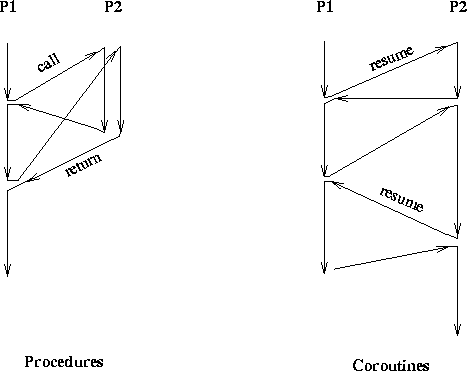
\includegraphics[width=3.9902in,height=3.1701in]{ub-img/ub-img8.png}
\end{center}

{\sffamily\bfseries Figure 4-1:}
{\sffamily The Difference Between Procedures and Coroutines}

\bigskip

Can you tell what the next example computes from its integer
command-line argument?

\bigskip

{\sffamily\bfseries
Listing 4-1}

{\sffamily\bfseries
Producer and Consumer Coroutines}

\iconcode{
procedure main(args) \\
\>   C1 := create consumer(args[1]) \\
\>   C2 := create producer(C1) \\
\>   @C2 \\
end \\
\ \\
procedure producer(ce) \\
\>   x := 1 \\
\>   repeat \{ \\
\>   \ \ \ val := x \^{} 2 \\
\>   \ \ \ ret := val @ ce {\textbar} break \\
\>   \ \ \ x +:= 1 \\
\>   \ \ \ \} \\
\>   @ \&main \\
end \\
\ \\
procedure consumer(limit) \\
\>   value := @ \&source \\
\>   repeat \{ \\
\>   \ \ \ \# process value \\
\>   \ \ \ if value {\textgreater} limit then break \\
\>   \ \ \ if value \% 2 = 0 then write(value) \\
\>   \ \ \ value := retval @ \&source \\
\>   \ \ \ \} \\
end
}

When producer resumes consumer, it passes \textsf{value}; the consumer
passes a return code (\textsf{retval}) back. \textsf{\&source} is the
coexpression that activated the current co-expression.

{\sffamily\bfseries
Note}

{\sffamily
This example doesn{\textquotesingle}t mean the producer/consumer problem
should always be done with coroutines!}

\subsubsection[Permutations]{Permutations}

\index{permutations}We have seen one usage of
\index{map()}\textsf{map()}, where it transformed mixed-case strings to
all lowercase. In that type of usage, the first string \ is the one
that we are manipulating, and the other two arguments tell it how the
string is to be modified. Interesting results can be achieved by
treating the \textit{third} argument as the string to manipulate.
Consider this code:

\iconcode{
s := {\textquotedbl}abcde{\textquotedbl} \\
write(map({\textquotedbl}01234{\textquotedbl},
{\textquotedbl}43201{\textquotedbl}, s))
}

What does this code example do? The transformation is:
\textsf{{\textquotedbl}4{\textquotedbl}} should be mapped to
\textsf{{\textquotedbl}a{\textquotedbl}},
\textsf{{\textquotedbl}3{\textquotedbl}} to
\textsf{{\textquotedbl}b{\textquotedbl}},
\textsf{{\textquotedbl}2{\textquotedbl}} to
\textsf{{\textquotedbl}c{\textquotedbl}},
\textsf{{\textquotedbl}0{\textquotedbl}} to
\textsf{{\textquotedbl}d{\textquotedbl}}, and
\textsf{{\textquotedbl}1{\textquotedbl}} to
\textsf{{\textquotedbl}e{\textquotedbl}}. When this mapping is applied
to \textsf{{\textquotedbl}01234{\textquotedbl}}, we get
\textsf{{\textquotedbl}edcab{\textquotedbl}} - a permutation of the
string \textsf{s}! It is exactly the permutation that is suggested by
the first two arguments of \textsf{map()}. To arrange this sort of
permutation, all three strings must be the same size, and there must be
no repeated letters in the second string.


\begin{center}
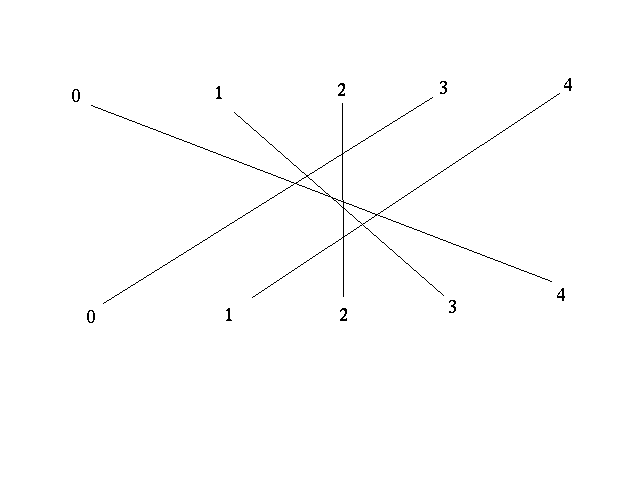
\includegraphics[width=5.0in,height=1.8in]{ub-img/ub-img9.png}
\end{center}
{\sffamily\bfseries Figure 4-2:}
{\sffamily Permuting a string with the map() function}

\bigskip

Here is an example: In the USA, dates are represented with the month
coming first, as in 12/25/1998, but in many other places the day comes
first: 25/12/1998. This conversion is, of course, just a permutation;
we can do this with a simple map:

\iconcode{
map({\textquotedbl}Mm/Dd/XxYy{\textquotedbl},
{\textquotedbl}Dd/Mm/XxYy{\textquotedbl}, date)
}

Here is another example. Unicon has a built-in random facility, the
\textsf{?} operator. Applied to a string or cset, it returns a random
character from the argument; applied to a structure, a random member of
that structure; and applied to an integer, a random integer between 1
and that number. This is a very useful feature and allows us to write
programs that shuffle cards or run simulations of things like rolling
dice.

By default in Unicon, the random sequence generated by \textsf{?} is
different for each run of the program. This is one of the few areas
where Unicon is deliberately different from Icon, which uses the same
seed each run by default. Icon{\textquotesingle}s semantics is good
when debugging, because we want the program to behave predictably while
it is broken! However, in most applications that use random numbers,
such as games, different runs of the program should create different
numbers. The \index{random!number seed}random number seed is keyword
\textsf{\&random.} It can be assigned a value at the start of main() in
order to get Icon-style repeatability. Here{\textquotesingle}s how to
assign it a number based on the current date and time.
Unicon{\textquotesingle}s default semantics do something similar.

\iconcode{
\&random := map({\textquotedbl}sSmMhH{\textquotedbl},
{\textquotedbl}Hh:Mm:Ss{\textquotedbl}, \&clock) +
map({\textquotedbl}YyXxMmDd{\textquotedbl},
{\textquotedbl}YyXx/Mm/Dd{\textquotedbl}, \&date)
}

The calls to \textsf{map()} remove punctuation characters from the
fixed-format strings produced by \textsf{\&clock} and \textsf{\&date}.
The resulting strings of digits are converted to integers, added, and
stored as a seed in \textsf{\&random}. Now every time the program is
run, the random number facility will be initialized with a different
number.

\subsection{Simulation}

A Galton Box is a device that demonstrates how balls falling through a
lattice of pegs will end up distributed binomially. A simulation of a
Galton box combines several of the techniques described previously.
\ Figure 4-3 is an illustration of the program{\textquotesingle}s
screen.



\begin{center}
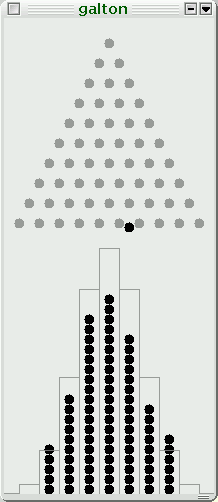
\includegraphics[width=1.75in,height=3.8201in]{ub-img/ub-img10.png}
\end{center}

{\sffamily\bfseries Figure 4-3:}
{\sffamily A Galton Box Simulation}

\bigskip

The simulation{\textquotesingle}s output window is a good example of
Unicon{\textquotesingle}s high-level graphics facilities. Graphics is a
broad area, discussed in Chapter 7 of this book; the on-line references
or the Icon graphics book (Griswold, Jeffery, Townsend 1998) contain
substantial additional details. Graphics are part of the system
interface. Some of the graphics functions used in this example include:

\begin{itemize}
\item \textsf{FillArc(x,y,width,height)} fills an ellipse defined by a
bounding rectangle. The shape is filled by the current foreground color
and/or fill pattern. The height defaults to be the same as the width,
producing a circle. Given additional arguments, \textsf{FillArc()
}fills parts of an ellipse similar to pieces of a pie in shape.
\item \textsf{WAttrib({\textquotedbl}attr{\textquotedbl})} or
\textsf{WAttrib({\textquotedbl}attr=value{\textquotedbl})}, the generic
routine for getting or setting a window{\textquotesingle}s attributes.
In this case the attributes \textsf{fg} (foreground color) and
\textsf{drawop} (raster drawing operation) are set to various colors
and reversible output.
\item \textsf{Window({\textquotedbl}attr=value{\textquotedbl}, ...)}
opens a window with initial characteristics as specified by a string of
attribute values. The \textsf{WDelay(t)} function waits until
\textsf{t} milliseconds have passed. The \textsf{WDone()} function
waits for the user to dismiss the output window by pressing
\textsf{{\textquotedbl}q{\textquotedbl}} and then terminates the
program and closes the window.
\end{itemize}
Listing 4-2 contains the code for a simplified version of the
simulation. A couple elements of the image above are omitted in order
to make the example easy to follow. (Both this program and the one that
created the screen shot above are included on the
book{\textquotesingle}s web site, http://unicon.sourceforge.net/book/)

{\sffamily\bfseries Listing 4-2}
{\sffamily\bfseries A Simple Galton Box Simulation}

\iconcode{
link graphics \\
global pegsize, height, width, pegsize2 \\
\ \\
procedure main(args) \\
local n, steps \\
\>   steps := 10 \\
\>   pegsize := 10 \\
\>   pegsize2 := pegsize * 2 \\
\>   n := integer(args[1]) {\textbar} 100 \\
\>   setup\_window(steps) \\
\>   every 1 to n do galton(steps) \\
\>   WDone() \\
end \\
\ \\
procedure setup\_window(n) \\
\ \\
local max, xpos, ypos, i, j \\
\>   \# Draw the n levels of pegs \\
\>   \# Pegboard size is 2n-1 square \\
\>   \# Expected max value of histogram is (n, n/2)/2\^{}n  \\
\>   \# ... approximate with something simpler? \\
\>   max := n*n/pegsize \\
\>   width := (2*n+1)*pegsize \\
\>   height := width + n*n/2*pegsize \\
\>   Window({\textquotedbl}size={\textquotedbl} {\textbar}{\textbar}
width {\textbar}{\textbar} {\textquotedbl},{\textquotedbl}
{\textbar}{\textbar} height, \\
\>   \ \ \ \ \ \ \ {\textquotedbl}fg=grayish-white{\textquotedbl}) \\
\>   WAttrib({\textquotedbl}fg=dark-grey{\textquotedbl}) \\
\>   every i := 1 to n do \{ \\
\>   \ \ \ ypos := i * pegsize2 \\
\>   \ \ \ xpos := width/2 - (i - 1) * pegsize - pegsize/2 \\
\>   \ \ \ every j := 1 to i do \{ \\
\>   \ \ \ \ \ \ FillArc(xpos, ypos, pegsize, pegsize) \\
\>   \ \ \ \ \ \ xpos +:= pegsize2 \\
\>   \ \ \ \ \ \ \} \\
\>   \ \ \ \} \\
\>   \# Set up drawing mode to draw the falling balls \\
\>   WAttrib({\textquotedbl}fg=black{\textquotedbl}) \\
\>   WAttrib({\textquotedbl}drawop=reverse{\textquotedbl}) \\
end
\ \\
\# Do it! \\
procedure galton(n) \\
local xpos, ypos, oldx, oldy \\
\>   xpos := oldx := width/2 - pegsize/2 \\
\>   ypos := oldy := pegsize \\
\>   \# For every ball... \\
\>   every 1 to n do \{ \\
\>   \ \ \ if ?2 = 1 then \\
\>   \ \ \ \ \ \ xpos -:= pegsize \\
\>   \ \ \ else \\
\>   \ \ \ \ \ \ xpos +:= pegsize \\
\>   \ \ \ ypos +:= pegsize2 \\
\>   \ \ \ animate(oldx, oldy, xpos, ypos) \\
\>   \ \ \ oldx := xpos \\
\>   \ \ \ oldy := ypos \\
\>   \ \ \ \} \\
\>   \# Now the ball falls to the floor \\
\>   animate(xpos, ypos, xpos, ypos + 40) \\
\ \ \ animate(xpos, ypos+40, xpos, ypos + 200) \\
\>   \# Record this ball \\
\>   draw\_ball(xpos) \\
end
\ \\
procedure animate(xfrom, yfrom, xto, yto) \\
\>   animate\_actual(xfrom, yfrom, xto, yfrom, 4) \\
\>   animate\_actual(xto, yfrom, xto, yto, 10) \\
end
\ \\
\# Drawing op is already set to {\textquotedbl}reverse{\textquotedbl},
and fg colour is black. \\
procedure animate\_actual(xfrom, yfrom, xto, yto, steps) \\
local x, y, xstep, ystep, i, lastx, lasty \\
\>   x := xfrom \\
\>   y := yfrom \\
\>   xstep := (xto - xfrom)/steps \\
\>   ystep := (yto - yfrom)/steps \\
\>   every i := 1 to steps do \{ \\
\>   \ \ \ lastx := x \\
\>   \ \ \ lasty := y \\
\>   \ \ \ FillArc(x, y, pegsize, pegsize) \\
\>   \ \ \ WDelay(1) \\
\>   \ \ \ FillArc(x, y, pegsize, pegsize) \\
\>   \ \ \ x +:= xstep \\
\>   \ \ \ y +:= ystep \\
\>   \ \ \ \} \\
end
\ \\
procedure draw\_ball(x) \\
static ballcounts \\
initial ballcounts := table(0) \\
\>   ballcounts[x] +:= 1 \\
\>   FillArc(x, height-ballcounts[x]*pegsize, pegsize, pegsize) \\
end
}

\section*{Summary}

Unicon is particularly powerful when different language features are
combined. The ability to combine features in interesting ways is the
result of its novel expression semantics. Co-expressions add
substantial value to the concept of \index{generator}generators,
although most programs use them only sparingly. They fit well into a
philosophy that says that simple things should be easy to do...and
complex things should be easy to do as well.



\chapter{The System Interface}

The \index{system interface}system interface is Unicon's connection to the
outside world, defining \index{input}input/\index{output}output interactions
with the operating system. This chapter shows how to
\begin{itemize}\itemsep0pt
  \item Manipulate \index{file}files, \index{directories}directories, and
    access \index{permissions, file access}permissions
  \item Launch and interact with other programs
  \item Handle abnormal events that would otherwise terminate your program
  \item Write \index{Internet}Internet \index{client}client and
    \index{server}server applications.
\end{itemize}

\section{The Role of the System Interface}

Unicon's predecessor Icon is highly portable; it runs on everything
from mainframes to Unix machines to Amigas and Macs. This platform
independence is both a virtue and a limitation. Icon takes a greatest
common denominator approach to the system interface. Icon programs run
with no source modifications across platforms, but with little access
to the underlying system. Icon historically could not be used easily
for many tasks such as system administration or client/server
programming. Both the Icon graphics facilities, and now the Unicon
system interface, "raise the bar" of what portable facilities
programmers can expect to be provided by their programming language,
at the cost of making it more difficult to port the language to new
platforms.

The interface described in this chapter relies on underlying standards
including ANSI C's standard library, and the IEEE Portable Application
Standards Committee's \index{POSIX}POSIX operating system standard
(http://www.pasc.org). Unicon relies on standards, but is simpler and
higher level. It is also less platform-specific than the POSIX
standard. The goal was to define facilities that can be implemented to
a great extent on all modern operating systems.  Non-POSIX Unicon
implementations may provide a subset of the functionality described in
this chapter, but important facilities such as TCP/IP Internet
communications are ubiquitous and warrant inclusion in the language
definition. So far the complete Unicon system interface is implemented
for Linux, Solaris, and Windows; the challenge to port these
facilities to all platforms on which they are relevant and useful now
rests with Unicon's user community.

\section{Files and Directories}

The file type is used for any connection between a program and an
external piece of hardware. In reality, a file is a
\index{reference!file}reference to resources allocated by the
operating system for the purpose of input or output. Different kinds
of files support different operations, but most files support the
basic functions given in this section.

Files are commonly used to manipulate named repositories of data on a
storage device. The contents of files exist independent of the program
that creates them, and persist after that program finishes.  To read
data from a file or save data to a file, the functions
\index{read()}\texttt{read()} and \index{write()}\texttt{write()} are
often used. These functions by default use special files denoted by
the keywords \index{input, standard \&input}\texttt{\&input} and
\index{output, standard \&output}\texttt{\&output},
respectively. There is a third file keyword, \index{error!standard,
\&errout}\texttt{\&errout}, that refers to the location to which the
program should write any error messages.  Unless the files were
redirected, they refer to the \index{keyboard}keyboard and the
\index{display}display. If you pass \texttt{read()} or
\texttt{write()} a value of type \textit{file} as an argument, the
operation is performed on that file. The function
\texttt{open()}\texttt{ }creates a value of type file:

\iconcode{
f := open("myfile.txt", "w") \\
write(f, "This is my text file.")
}

\noindent
The \index{open()}\texttt{open()} function takes two parameters: a file
name and a mode. The default mode is
\texttt{"r"} for reading; the example above
uses mode \texttt{"w"} for
writing. Other modes denote other kinds of system interfaces.
They are described in later sections.

The \texttt{read()} function reads and returns a line of text, removing the
line terminator(s). Function \texttt{write()}
similarly adds a line terminator after writing its arguments.
Another way to read lines is via the generate operator, unary
\texttt{!}. The expression \texttt{!f} generates the lines of file
\texttt{f}, so \texttt{every put(L, !f)} puts the lines of
\texttt{f} into list \texttt{L}.

On systems with multi-character line terminators, appending an
extra letter to the mode parameter of \texttt{open()} indicates whether
newlines are to be translated (mode
\texttt{"t"}) or untranslated (mode
\texttt{"u"}). Text files should
be translated, while binary files should not. The default is to translate
newlines to and from operating system format.

Besides \texttt{read()} and \texttt{write()}, which always process a
single line of text, the functions \texttt{reads(f, i)} and
\texttt{writes(f, s, ...)} read (up to \texttt{i} characters) and write
strings to a file. These functions are not line-oriented and do no
newline processing of their own, although they still observe the
translation mode on systems that use one.

When operations on a file are complete, close the file by calling
\index{close()}\texttt{close(f)}. The only exceptions are the standard
files, \texttt{\&input}, \texttt{\&output}, and \texttt{\&errout};
since you didn't open them, don't
close them. For the rest, most operating systems have a limit on the
number of files that they can have open at any one time, so not closing
your files can cause your program to fail in strange ways if you use a
lot of files.

\subsection{Directories}

A \index{directory}directory is a special file that contains a
collection of named files. Directories can contain other directories to
form a hierarchical structure. The \index{chdir()}\texttt{chdir()}
function returns the current working directory as an absolute path
name. Called with a string argument, the
\texttt{chdir(}\texttt{\textit{dirname}}\texttt{)} function sets the
current working directory to \texttt{dirname}. The call
\texttt{open(}\texttt{\textit{dirname}}\texttt{)} opens a directory to
read its contents. Directories can only be opened for reading,
not for writing. Every \texttt{read()} from a directory returns
the name of one file. Directory entries are not guaranteed to be in any
order. The expression \texttt{every
write(!open("."))} writes the names of the
files in the current directory, one per line. It is not good practice
to call an \texttt{open()} that you don't
\texttt{close()}.

The \index{mkdir()}\texttt{mkdir(s)} function creates a directory. An
optional second parameter specifies access permissions for
the directory; controlling file ownership and access is discussed
below. Files or directories can be renamed with \texttt{rename(s1,s2)}.
Renaming does not physically move the file, so if \texttt{s1} and
\texttt{s2} denote locations on different hardware devices or file
systems then \index{rename()}\texttt{rename()} will fail, and you will
need to "copy and then delete"
the file. Individual files or directories are removed with
\index{remove(s)}\texttt{remove(s)}. Only empty directories may be
removed. To remove an entire directory including its contents:

\iconcode{
procedure deldir(s) \\
\>   f := open(s) \\
\>   every remove( s {\textbar}{\textbar}
"/" {\textbar}{\textbar}
("." \~{}==
(".." \~{}== !f))) \\
\>   close(f) \\
\>   remove(s) \\
end
}

How would you change this function to delete subdirectories? You might
be able to devise a brute force approach using what you know, but what
you really need is more information about a file, such as whether it is
a directory or not.

\subsection{Obtaining file information}

\index{file!information}\textit{Metadata} is information about the file
itself, as opposed to information stored in the file. Metadata includes
the owner of the file, its size, user access rights,
and so forth. This information is produced by the
\index{stat(f)}\texttt{stat()} system call. Its argument is the name of
a file or (on UNIX systems only) an open file. The \texttt{stat()}
function returns a record with the information about the file. Here is
a subset of \texttt{ls}, a UNIX program that reads a directory and
lists information about its files. Keyword \index{errortext,
keyword}\texttt{\&errortext} contains information about the
most recent error that resulted in an expression
\index{fail!expression}failure; it is written if opening the directory
fails. This version of \texttt{ls} only works correctly if its
arguments are the names of directories. How would you modify it, using
\texttt{stat()}, to take either ordinary file names or directory names
as command line arguments?

\iconcode{
link printf \\
procedure main(args) \\
\>   every name := !args do \{ \\
\>   \ \ \ f := open(name) {\textbar} stop(\&errortext, name) \\
\>   \ \ \ L := list() \\
\>   \ \ \ while line := read(f) do \\
\>   \ \ \ \ \ \ push(L, line) \\
\>   \ \ \ every write(format(stat(n := !sort(L)), n)) \\
\>   \ \ \ \} \\
end \\
procedure format(p, name) \\
\ \ \ s := sprintf("\%-7d \%-5d \%s \%-4d \%-9d \%-9d
\%-8d \%s \%s",  \\

\ \ \ \ \ \ \ \ \ \ p.ino, p.blocks, p.mode, p.nlink, p.uid, p.gid,
p.size, \\

\ \ \ \ \ \ \ \ \ \ ctime(p.mtime)[5:17], name) \\
\>   if p.mode[1] == "l" then \\
\>   \ \ \ s {\textbar}{\textbar}:= " -{\textgreater}
" {\textbar}{\textbar} {\textbackslash}(p.symlink) \\
\>   return s \\
end
}

The record returned by \texttt{stat()} contains many fields. Not all file
systems support all of these fields. Two of the most important portable fields
are \texttt{size}, the \index{file size}file size in bytes, and \texttt{mtime},
the file's last \index{file!modified time}modified time, an integer that is
converted into a human readable string format by \texttt{ctime(i)}. Another
important field is \texttt{mode}, a string that indicates the file's type and
\index{access, file}access permissions. Its first letter (\texttt{mode[1]}) is
\texttt{"-"} for normal files, \texttt{"d"} for directories, and some file
systems support additional types. The other characters of the mode string are
platform dependent. On UNIX there are nine letters to encode read, write, and
execute permissions for user, group, and world, in the format:
\texttt{"rwxrwxrwx"}. On a classic Windows FAT file system, there is only
\texttt{"rwa"} to indicate the status of hidden, read-only, and archive bits (if
it is set, the system bit is indicated in \texttt{mode[1]}).

Some file systems support duplicate directory entries called
\textit{links} that refer to the same file. In the record returned by
\texttt{stat()}, a \index{link, file system}link is indicated by a
\texttt{mode[1]} value of \texttt{"l"}. In addition, field
\texttt{nlinks} ("number of links") will be \texttt{{\textgreater} 1}
and/or field \texttt{symlink} may be the string filename of which this
file is an alias. Appendix E includes information on each platform's
support for the \texttt{mode} field, as well as \texttt{stat()}'s
other fields.

\subsection{Controlling file ownership and access}

\index{file ownership}The previous section shows how different
platforms' file systems vary in their support for the concepts of file
ownership and access. If the system supports ownership, the user and
group that own a file are changed by calling \texttt{chown(fname,
user, group)}. The \index{chown()}\texttt{chown()} function only
succeeds for certain users, such as the super user.  User and group
may be string names, or integer user identity codes on some platforms.

File access rights are changed with \texttt{chmod(fname, mode)}. The
\index{chmod()}\texttt{chmod()} function only succeeds for the owner of a given
file. The \texttt{mode} is a nine-letter string similar to \texttt{stat()}'s
mode field, or an octal encoding of that information (see Appendix E).

Another piece of information about files is called the
\index{umask}\textit{umask}. This is a variable that tells the system what
access rights any newly created files or directories should have.  The function
call \texttt{umask("rwxr-xr-x")} tells the system that newly created directories
should have a permission of \texttt{"rwxr-xr-x"} and files should have
permissions of \texttt{"rw-r-{}-r-{}-"}.  The \texttt{mkdir(s, mode)} function
takes an optional mode parameter, which can override the umask for for newly
created directories.  Ordinary files are never given execute permission by the
system, it must be set explicitly with \texttt{chmod()}.

\subsection{File locks}

Files can be \index{file!lock}locked while a program is updating some
information. If the contents of the file are in an inconsistent state, other
programs may be prevented from reading (or especially writing) the
file. Programs can cooperate by using file locks:

\iconcode{
flock(filename, "x")}

\noindent
The first call to \texttt{flock()} creates a lock, and subsequent
calls by other programs will block, waiting till the
writing program releases its lock. The flag
\texttt{"x"} represents an
\textit{exclusive} lock, which should be used while writing; this means
no other process can be granted a lock. For reading,
\texttt{"s"} should be used to create a
shared lock so that other programs that are also just reading can do
so. In this way you can enforce the behavior that only one process may
open the file for writing, and all others will be locked out; but many
processes can concurrently open the file for reading.

\section{Programs and Process Control}

Unicon's system interface is similar but
higher level than the POSIX C interface. An include file
\texttt{posix.icn} defines constants used by some functions. Include
files are special code, consisting mainly of defined symbols, intended
to be textually copied into other code files. They are handled by the
preprocessor, described in Appendix A. To include \texttt{posix.icn} in
a program, add this line at the top of your program:

\iconcode{
\$include "posix.icn"}

When a system call \index{fail!system call}fails, the integer keyword
\texttt{\&errno} indicates the error that occurred. As seen earlier, a
human-readable string is also available in \index{errortext,
keyword}\texttt{\&errortext}. Error codes (such as \texttt{EPERM}, or
\texttt{EPIPE}) are defined in \texttt{posix.icn}; \index{errno,
keyword}\texttt{\&errno} can be compared against constants like
\texttt{ENOENT}. In general, however, human readers will prefer to
decipher \texttt{\&errortext}.

In the discussion to follow, a \textit{program} is the code, while
a \index{process}\textit{process} is such
a program in execution. This distinction is not usually important, but
for network applications it matters,
since the same program can run in multiple processes, and a process can
change the program that it is running.

\subsection{Signals}

A \index{signal}signal is an asynchronous message sent to a process either by
the system (usually as a result of an illegal operation like a
\index{error!floating point}floating point error) or by another process. A
program has two options to deal with a signal: it can allow the system to handle
it in the default manner (which may include termination of the process) or it
can register a function, called a signal handler, to be run when that signal is
delivered.

Signals are trapped or ignored with the \texttt{trap(s, p)} function.  Argument
\texttt{s} is the string name of the signal. The signal names vary by platform;
see Appendix E. You can trap any signal on any machine; if it is not defined it
will be ignored. For example, Linux systems don't have a \texttt{SIGLOST.}
Trapping that signal has no effect when a program runs on Linux. The
\texttt{trap()} function's second argument is the procedure to call when the
signal is received. The previous signal handler is returned from
\index{trap()}\texttt{trap()} so it can be restored by a subsequent call to
\texttt{trap()}. The signal handler defaults to the default provided by the
system. For instance, \texttt{SIGHUP} is ignored by default but \texttt{SIGFPE}
will cause the program to terminate.

Here is an example that handles a \texttt{SIGFPE} (floating point exception) by
printing out a message and then runs the system default handler:

\iconcode{
global oldhandler \\
\>   ... \\
\>   trap("SIGFPE", sig\_ignore) \\
\>   oldhandler := signal("SIGSEGV",
handler) \\
\>   ... \\
\ \ \ \# restore the old handler \\
\>   trap("SIGSEGV", oldhandler) \\
end \\
\ \\
procedure sig\_ignore(s); end
\ \\
procedure handler(s) \\
\>   write(\&errout, "Got signal ", s) \\
\>   ({\textbackslash}oldhandler)(s) \\
\ \ \ \ \ \ \ \ \ \ \ \ \ \ \ \ \ \# propagate the signal \\
end
}

\subsection{Launching programs}

Many applications execute other programs and read their results. In many cases,
the best way to do this is to call \texttt{open()} with mode \texttt{"p"}
(\index{pipe}pipe) to launch a command. In mode \texttt{"p"} the string argument
to \texttt{open()} is not a filename, it is an entire command string. Piped
commands opened for reading (mode \texttt{"p"} or \texttt{"pr"}) let your
program read the command's standard output, while piped commands open for
writing (mode \texttt{"pw"}) allow your program to write to the command's
standard input.

The more general function \texttt{system(x,f1,f2,f3,mode)} runs an external
command (argument \texttt{x}) with several options. If \texttt{x} is a list,
\texttt{x[1]} is the command to execute and the remaining list elements are its
command line arguments. If \texttt{x} is a string, it is parsed into arguments
separated by spaces. Arguments with spaces in them may be escaped using double
quotes. A program that calls \index{system()}\texttt{system()} normally waits
for the launched program to complete before continuing, and \texttt{system()}
returns the integer status of the completed command. If \texttt{s} ends in an
ampersand (\texttt{\&}) or the optional \texttt{mode} argument is \texttt{1} or
\texttt{"nowait"}, \texttt{system()} does not wait for the command to complete,
but instead launches the command in the background and returns an integer
process id. The \texttt{system()} function takes three optional file arguments
that specify redirected standard input, output, and error files for the launched
program.

\subsection{Using file redirection and pipes}

\index{file!redirection}One common scenario is for a program to run
another program but with the input and output redirected to files. On
command-line systems like the Unix shells or the MS-DOS command prompt,
you may have used redirection:

\iconcode{
\ \ \ prog {\textless} file1
}

\noindent
File redirection characters and other platform-dependent operations are
supported in the command string passed to \texttt{system()}, as
in the following \texttt{system()} call:

\iconcode{
\>   system("prog {\textless} file1")
}

Pipes to and from the current program are nicely handled by the
\texttt{open()} function, but sometimes the input of one program needs
to be connected to the output of another program. You may have seen
uses like this:

\iconcode{
prog1 {\textbar} prog2
}

The \texttt{pipe()} function returns a pair of open files in a list,
with the property that anything written to the second file will appear
on the first. Here's how to hook up a pipe between two
programs:

\iconcode{
\>   L := pipe() {\textbar}
stop("Couldn't get pipe: ", \&errortext) \\
\>   system("prog1 \&", , L[2]) \\
\>   system("prog2 \&", L[1]) \\
\>   close(L[1]) \\
\>   close(L[2])
}

\subsection{Process information}

The integer process identity can be obtained with
\index{getpid()}\texttt{getpid()}. The user id of the process can be
obtained with \index{getuid()}\texttt{getuid()} if the platform
supports it. Calls to obtain additional information such as group
identity on some platforms are described in Appendix E.

A parent process may want to be notified when any of its children quit
(or change status). This status can be obtained with the function
\index{wait()}\texttt{wait()}. When a child process changes state from
``running'' to either
``exited'' or
``terminated'' (and optionally
``stopped''), \texttt{wait()} returns a
string of the form

\iconcode{
pid:status:arg:core}

The \texttt{":core"} will only be present if
the system created a core file for the process. The status can be any
of \texttt{``exited''},
\texttt{``terminated''} or
\texttt{``stopped''}. The \texttt{arg} field
is either: a) the exit status of the program if it exited; or b) the
signal name if it was terminated. Typically \texttt{wait()} will be
used in the handler for the \texttt{SIGCHLD} signal which is sent to a
process when any of its children changes state.

The arguments to \texttt{wait()} are the pid of the process to wait for
and any options. The default for pid is to wait for all children. The
options may be either \texttt{"n"}, meaning
\texttt{wait()} should not wait for children to block but should return
immediately with any status that's available, or
\texttt{"u"}, meaning that any processes
that stopped should also be reported. These options may be combined by
using \texttt{"nu"}.

\subsection{The \texttt{select()} system call}

Some programs need to be able to read data from more than one source.
For example, a program may have to handle network traffic and also
respond to the \index{keyboard}keyboard. The problem with using
\texttt{read()} is that if no input is available, the program will
block and will not be able to handle the other stream that may in fact
have input waiting on it. To handle this situation, you can use the
function \texttt{select(x1,x2,...i)}. The
\index{select()}\texttt{select()} function tells the system which files
you are interested in reading from, and when input becomes available on
any of those sources, the program will be notified. The
\texttt{select()} function takes files or lists of files as its
arguments, and returns a list of all files on which input is waiting.
If an integer argument is supplied, it is a timeout that gives the
maximum milliseconds to wait before input is available. If the timeout
expires, an empty list is returned. If no timeout is given, the program
waits indefinitely for input on one of the files.

\iconcode{
while *(L := select(f1, f2, f3, timeout)) = 0 do \\
\> handle\_timeout() \\
(\&errno = 0) {\textbar} stop("Select
 \index{expression failure}failed: ", \&errortext) \\
every f := !L do \{ \\
\> \# Dispatch reads pending on f \\
\> ... \\
\> \}
}

When using \texttt{select()} to process input from multiple files, you
may need to pay some attention to avoid blocking on any one of your
files. For example the function \texttt{read()} waits until an entire
line has been typed and then returns the whole line. Consider this
code, which waits for input from either a file (or network connection)
or a window designated by keyword \texttt{\&window}:

\iconcode{
\ \ \ while L := select(f, \&window) do \\
\ \ \ \ \ \ if !L === f then c := read(f)
}

Just because \texttt{select()} has returned doesn't
mean an entire line is available; \texttt{select()} only guarantees
that at least one character is available. The command shell log
application in Chapter 14 shows the usage of \texttt{select()}. Another
primary application area for \texttt{select()} is network programming,
described later in this chapter. For network connections, the function
\texttt{reads(f, i)} will return as soon as it has some input
characters available, rather than waiting for its maximum string size
of \texttt{i}. But if no input is available, reads() blocks.

\subsection{Non-blocking input and the \texttt{ready()} function}

The function \texttt{ready(f, i)} is like \texttt{reads(f, i)} except
that it is non-blocking, that is, it returns immediately with up to
\texttt{i} bytes if they are available, but it does not wait around. It
is ideal for use with \texttt{select()} and in situations where a
server or client needs to interact with multiple remote connections.

\section[Networking]{Networking}
\index{networking}Unicon provides a very high-level interface to
\index{Internet}Internet communications. Applications with custom
communications use one of the major Internet
applications protocols, \index{TCP}TCP and UDP. An higher level
interface to several popular Internet protocols such as HTTP and POP is
provided by means of Unicon's messaging facilities.

\subsection{TCP}

A TCP connection is a lot like a phone call: to make a connection you
need to know the address of the other end, just like a phone number.
For TCP, you need to know the name of the machine to connect to, and an
address on that machine, called a \textit{port}. A server listens for
connections to a port; a client sends requests to a port. Also, there
are two kinds of ports, called "Internet
Domain" and "Unix Domain."
The distinction is beyond the scope of this book; we will just mention
that Internet Domain ports are numbers, and Unix Domain ports look like
files. Also, a connection to a Unix domain port can only be made from
the same machine, so we will not consider the Unix domain further here.

A call to \texttt{open()} with mode
\texttt{"n"} (network) requests a network
connection. The first argument to \texttt{open()} is the network
address, a host:port pair for Internet domain connections, and a
filename for Unix domain sockets. If the address contains no host name
and therefore starts with \texttt{":"}, the
socket is opened on the same machine. The value returned by
\texttt{open()} is a file that can be used in \texttt{select()} and
related system functions, as well as normal reading and writing. 

A \index{client}client uses mode
\texttt{"n"} with \texttt{open()} to open a
connection to a TCP server. Here is a simple version of the Internet
"finger" program:

\iconcode{
procedure main(argv) \\
\>   local fserv := getserv("finger")
{\textbar} \\
\>   \ \ \ stop("Couldn't get service:
", \&errortext) \\
\>   name := argv[1] \\
\>   host := "" \\
\>   argv[1] ? \{ \\
\>   \ \ \ name := tab(find("@")) \&
="@" \& host := tab(0) \\
\>   \ \ \ \} \\
\>   if *host {\textgreater} 0 then
write("[", host,
"]") \\
\>   f := open(host {\textbar}{\textbar}
":" {\textbar}{\textbar} fserv.port,
"n") {\textbar} \\
\>   \ \ \ stop("Couldn't open
connection: ", \&errortext) \\
\ \\
\>   write(f, name) {\textbar}
stop("Couldn't write: ",
\&errortext) \\
\>   while write(read(f)) \\
end
}

Notice the use of \index{getserv()}\texttt{getserv()}. The
\texttt{posix\_servent} record it returns includes fields for the name,
aliases, port, and protocol used by the Internet service indicated in
\texttt{getserv()}'s argument. The Internet protocols
specify the ports to be used for various services; for instance, email
uses port 25. Instead of having to remember port numbers or hard-coding
them in our program, we can just use the name of the service and have
\texttt{getserv()} translate that into the port number and protocol we
need to use.

To write a \index{server}server, all we need to do is add
\texttt{"a"} (accept) to the mode after the
\texttt{"n"} in \texttt{open()}. Here is a
simple TCP server that listens on port 1888:

\iconcode{
procedure main() \\
\>   while f := open(":1888",
"na") do \{ \\
\>   \ \ \ system("myserverd -servicerequest
\&", f, f) \\
\>   \ \ \ close(f) \\
\>   \ \ \ \} \\
\>   (\&errno = 0) {\textbar} stop("Open failed:
", \&errortext) \\
end
}

The call \texttt{open(":1888",
"na")} blocks until a client connects.
The returned value is a file that represents the network connection.
This example server
responds to requests by launching a separate process to handle each
request. The network connection is passed to \texttt{myserverd} as its
standard input and output, so that process had better be expecting a
socket on its standard I/O files, and handle it appropriately.
This works on UNIX; on other platforms a different approach is needed.

Launching a separate process to handle requests is standard operating
procedure for many Internet servers, but besides the portability
concerns, it uses a lot of memory and CPU time. Many servers can be
implemented in a single process. Chapter 15 includes an example of such
a server. \ Mode \texttt{"na"} is less than
ideal for one-process servers: it only supports one connection at a
time. When waiting for a new connection, the process is not doing any
computation, and when servicing a connection, the program is not
listening for any other connection requests. Unless each connection is
of short duration, the server will appear to be down, or appear to be
unacceptably slow, to anyone trying to connect while an existing
request is being processed.

\subsection{Determining IP numbers}

Many programs need the IP number of the machine they are talking to. Given a
network connection {\texttt f}, \index{image()}\texttt{image(f)} will show the
IP address and port of the client machine that is connected (this is sometimes
called the \index{peername}\textit{peername}).

Some programs need to know their own IP number, but each machine can have
several IP numbers, one for each kind of physical network hardware in operation.
To obtain a list of local IP numbers, a program can read the output of
\texttt{/sbin/ifconfig} (UNIX) or \texttt{ipconfig} (Windows). To find the IP
number used for a particular network connection \texttt{n}, on some platforms
you can call \texttt{gethost(n)}, which returns a string with the IP number and
port used by the local machine for a given connection.

If you do determine your IP number in one of these ways, it is usually not the
number seen by the world, because most devices are connecting through some form
of network address translation.  To see the number that the world sees, you have
to connect to someone else and ask them to tell you what IP number they see you
at.

\iconcode{
procedure main(argv) \\
\>   n := open(argv[1],"n") | \\
\>\>      stop("can't connect to ", argv[1]|"missing host") \\
\>   write("connected to: ", image(n)[6:-1]) \\
\>   write("using: ", gethost(n)) \\
end
}

\subsection{Non-blocking network \texttt{open}s}

Servers need to never block. The call
\texttt{open(":port","nl")}
creates a \textit{listener} on the specified port, without waiting around for
someone to actually connect to it. The network file returned from
\texttt{open()} is not open for reading or writing, so it is not good for
much...yet. About the only thing you can do with such a file is include it
(along with any other network connections you have going) as an argument in a
call to \texttt{select()}. If a listener matches a current connection request,
\texttt{select()} converts it into a regular network connection as per mode
\texttt{"na"}.

In addition to non-blocking servers' listener connections, in the real-world
clients need a way to do an almost non-blocking connection as well.
TCP connections over long distances take a highly variable amount of time,
but most clients do not want to ``freeze'' for a couple of minutes while
the connection attempt times out. The network client versions of \texttt{open()}
allows an optional third parameter to supply it with a timeout value,
in milliseconds.

\subsection{UDP}

\index{UDP}UDP is another protocol used on the Internet. TCP is like a
phone call: all messages you send on the connection are guaranteed to
arrive in the same order they were sent. UDP on the other hand is more
like the postal service, where messages are not guaranteed to reach
their destination and may not arrive in the same order they were sent
in. Messages sent via UDP are called \textit{datagrams}.
It's a lot cheaper (faster) to send UDP messages than
TCP, though, especially if you are sending them across the Internet
rather than to a local machine. Sending a postcard is usually cheaper
than a long distance phone call!

UDP datagrams can be sent either with an \texttt{open()/writes()}
pair, or with \texttt{send()}. Typically a server sends/receives on the
same socket so it will use \texttt{open()} with \texttt{read()} and
\texttt{write()}. A client that only sends one or two datagrams uses
\index{send()}\texttt{send()}\texttt{/}\index{receive()}\texttt{receive()}.

The following example provides a service called
"rdate" that allows a program to ask a
remote host what time it has. The server waits for request datagrams
and replies with the date and time. The
\texttt{"u"} flag added to the mode in the
call to \texttt{open()} signifies that a UDP connection should be used.
The function \texttt{receive()} waits for a datagram to arrive, and
then it constructs a record having the address the message came from
and the message in it. The server uses the address to send the reply.

\iconcode{
\ \ \ f := open(":1025",
"nua") \\
 \ \ while r := receive(f) do \{ \\
\ \ \ \ \ \ \# Process the request in r.msg \\
\ \ \ \ \ \ ... \\
\ \ \ \ \ \ send(r.addr, reply) \\
\ \ \ \ \ \ \}
}

The record returned by \texttt{receive()} has two fields: the
\texttt{addr} field contains the address of the sender in
\texttt{"}\texttt{\textit{host}}\texttt{:}\texttt{\textit{port}}\texttt{"}
form, and the \texttt{msg} field contains the message.

To write a UDP client, use mode \texttt{"nu"}
Since UDP is not reliable, the \texttt{receive()} is guarded
with a \texttt{select()}; otherwise, the program might hang forever if
the reply is lost. The timeout of five seconds in the call to
\texttt{select()} is arbitrary and might not be long enough on a
congested network or to access a very remote host. Notice the second
argument to \texttt{getserv()}; it restricts the search for Internet
service information to a particular network protocol, in this case UDP.

\iconcode{
procedure main(args) \\
\>   (*args = 1) {\textbar} stop("Usage: rdate
host") \\
\>   host := args[1] \\
\>   s := getserv("daytime",
"udp") \\
\>   f :=
open(host{\textbar}{\textbar}":"{\textbar}{\textbar}s.port,
"nu") {\textbar} \\
\>   \ \ \ stop("Open failed: ",
\&errortext) \\
\>   writes(f, " ") \\
\>   if *select(f, 5000) = 0 then \\
\>   \ \ \ stop("Connection timed out.") \\
\>   r := receive(f) \\
\>   write("Time on ", host,
" is ", r.msg) \\
end
}

From these examples you can see that it is relatively easy to write
programs that use Internet communication. But TCP and UDP are very
general, somewhat low-level protocols; most programs employ a
higher-level communication protocol, either by defining their own, or
using a standard protocol. If you need to define your own Internet
protocol, you can do it on top of TCP or UDP; if your program needs to
use a standard Internet protocol, you should check first to see if the
protocol is built-in to the language as part of the messaging
facilities, described in the next section.

\section{Messaging Facilities}

Unicon's \index{messaging}messaging facilities provide
higher level access to many popular Internet protocols. A call to
\texttt{open()} using mode \texttt{"m"}
establishes a messaging connection. The filename argument to a
messaging connection is a URI (Uniform Resource Indicator) that
specifies the protocol, host machine, and resource to read or write.
The protocols implemented thusfar are HTTP, Finger, SMTP, and POP.
Extra arguments to open() are used to send headers defined by the
protocol. For example, the call

\iconcode{
open("mailto:unicon-group", "m", "Reply To: jeffery@cs.uidaho.edu")}

\noindent
supplies a Reply To field as a third parameter to \texttt{open()} on an
SMTP connection.

Header fields from the server's response to a
connection are read by subscripting the message connection value
with a string header name; an example is in the next section.

\subsection{HTTP}

\index{HTTP}HTTP is used to read or write to Web servers; the content
read or written typically consists of \index{HTML}HTML text. The
following program, \texttt{httpget.icn}, fetches a remote file
specified by a URI on the command line, and saves it as a local file.
The Icon Program Library module \texttt{basename} is used to extract
the filename from the URI.

\iconcode{
link basename}

\iconcode{
procedure main(argv) \\
\>   f1 := open(argv[1],"m") \\
\>   f2 := open(basename(argv[1]),"w") \\
\>   while write(f2, read(f1)) \\
end
}

This example retrieves the actual data for a successful HTTP request;
for a failed request the connection returns no data, appearing to be an
empty file. Programs can check the HTTP status code in order to
determine the nature of the problem. Status codes and other metadata
from HTTP header lines are inspected by subscripting the connection
with the desired header. For example, in the previous program, checking
\texttt{f1["Status-Code"]} would allow us
to detect HTTP errors, and
\texttt{f1["Location"]} would allow us to
find the new location of the file, if the HTTP server had informed us
that the file had moved. You can retrieve this status information on a
remote file without retrieving the file itself. If you open a URI with
mode \texttt{"ms"} instead of
\texttt{"m"}, an HTTP request for header
information is made, but no data is retrieved.

\subsection{SMTP and POP}

\index{SMTP}SMTP is used to send a mail message. Mail is delivered via
an SMTP server machine on which the user must have a valid account.
These default to the current user on the current host machine. Two
environment variables UNICON\_SMTPSERVER and UNICON\_USERADDRESS can be
set to override the default behavior.

\index{POP}POP is used to read mail messages. POP is the least file-like
of these protocols. A POP connection feels like a list of strings, each
string containing an entire mail message, rather than a simple sequence
of bytes. Function \texttt{read()} and operator \texttt{!} produce
entire messages which in general contain many newline characters. POP
messages may be removed by either \index{delete()!from POP
mail}\texttt{delete()} or \index{pop()!from POP mail}\texttt{pop()};
messages are buffered in such a way that message removal on the server
occurs when the connection is explicitly and successfully closed.

Here's a simple program that illustrates the use of
msesaging to get email from a POP server. It gets messages from the
server without deleting them and, for every message, prints out who the
message is from as well as the subject line.

\iconcode{
procedure main(argv) \\
\>   user := argv[1] {\textbar}
getenv("USER") {\textbar}
stop("no user") \\
\>   passwd := argv[2] {\textbar}
getenv("PASSWD") {\textbar}
stop("no password") \\
\>   server := argv[3] {\textbar}
getenv("MAILHOST") {\textbar}
"mailhost" \\
\>   conn :=
open("pop://"{\textbar}{\textbar}user{\textbar}{\textbar}":"{\textbar}{\textbar}passwd{\textbar}{\textbar}"@"{\textbar}{\textbar}server,
"m") {\textbar} \\
\>   \ \ \ stop("couldn't connect to
the POP server ", server) \\
\>   every msg := !conn do msg ? \\
\>   \ \ \ while line :=
tab(find("{\textbackslash}n")) do \\
\>   \ \ \ \ \ \ if =("From: "
{\textbar} "Subject: ") then
write(line) \\
\>   close(conn) \\
end
}

\noindent
You should improve the password handling in this program if you use it!
Chapter 14 includes another example use of
Unicon's POP messaging facilities: a spam filter.

\section{Tasks}

A task is the virtual machine execution state of a program. The tasking
facilities allow Unicon programs to load, execute, communicate with,
and control one another, all within a single instantiation of the
Unicon interpreter. 
Although Unicon programs can use the tasking facilities to load and
execute any number of other programs within the same interpreter space,
the tasking facilities do not introduce a concurrent programming
construct nor do they include special support for multiprocessor
hardware. Their domain is that of high-level language support for
programs that benefit from or require a tighter coupling than that
provided by inter-process communication; that is, programs that access
each other's state extensively.

Co-expressions provide the tasking facilities' program
execution model, and co-expression activation serves as the
communication mechanism. The extensions are general enough to be useful
in a wide variety of contexts. For example, programs that use the
multi-tasking interface can communicate directly without resorting to
external files or pipes.

At the language level, the tasking facilities consist of several
built-in functions and keywords, but no new types, declarations, or
control structures. Several existing functions have been extended to
offer additional support for the multi-tasking environment. 
Separate memory allocation regions are established for each task. 

\subsection{Preliminary terminology}

Before describing the task model, a few definitions are needed. These
definitions pertain to regions of memory referenced by programs during
execution. 

A \textit{name space} is a mapping from a set of program source-code
identifiers to a set of associated memory locations [Abelson85]. Icon
programs have a global name space shared across the entire program and
various name spaces associated with procedures. Procedures each have a
static name space consisting of memory locations shared by all
invocations of the procedure and local name spaces private to each
individual invocation of the procedure.
When a co-expression is created, a new local name space is allocated for
the currently executing procedure, and the current values of the local
variables are copied into the new name space for subsequent use by the
co-expression. 

An Icon program has an associated \textit{program state} consisting of
the memory associated with global and static name spaces, keywords, and
dynamic memory regions. Similarly, a co-expression has an associated
\textit{co-expression state} consisting of an evaluation stack that
contains the memory used to implement one or more local name spaces.
Co-expressions in an Icon program share access to the program state and
can use it to communicate. 

\subsection{Tasks as an extended co-expression model}

A task is the execution state of a program within the virtual machine
[Griswold86]. A single task called the root is created when the
interpreter starts execution. Additional tasks can be created
dynamically as needed.
A task consists of a main co-expression and zero or more child
co-expressions that share a program state. At the source-language
level, tasks are loaded, referenced, and activated solely in terms of
one of their member co-expressions; the task itself is
implicit.

This definition of tasks is related to the concept of the same name
commonly used in operating systems and concurrent programming
languages. It differs, however, in certain fundamental respects. Icon
is a sequential language; co-expressions in Icon provide a synchronous
coroutine execution model, not a concurrent execution model with
implicit task switching and scheduling. Another way to view this is
that unlike other languages such as Ada, Unicon provides the task model
as a mechanism for multi-tasking, but does not predefine the policy;
matters such as the scheduling algorithm used and whether multi-tasking
is co-operative or pre-emptive are programmable at the user
level.

Another useful comparison can be made between Icon tasks and Smalltalk
processes. Both provide pseudo-concurrency within the context of a
sequential virtual machine. Since Unicon tasks have their own dynamic
memory regions, their presence affects each other less than Smalltalk
processes affect each other. For example, if one task is exhibiting
thrashing heap behavior in which garbage collections are frequent, the
other tasks in the system can execute at full speed during the portion
of time in which they are running, since they do not allocate memory
out of the thrashing task's (full) heap. This minimal
effect of tasks on each others' behavior is especially
important in the domain of execution monitoring. 

\subsection{Task creation}

A task can create other tasks. The function 

\iconcode{
load(s, L, f1, f2, f3, i1, i2, i3)}

\noindent loads an icode file [Griswold86] specified by the file name
\textrm{s}, creates a task for it and returns a co-expression corresponding to
the invocation of the procedure {\textrm{main(L)}} in the
loaded icode file.  {\textrm{L}}{
}defaults to the empty list. Unlike conventional Icon command-line argument
lists, the argument list passed to{
}{\textrm{load()}} can contain values of any type, such as
procedures, lists, and tables in the calling task.

The task being loaded is termed the child task, while the task calling
{\textrm{load()}} is termed the parent. The
collection of all tasks forms a tree of parent-child
relationships.

{\texttt{f1}}, {\texttt{f2}},
and {\texttt{f3}}{ }are file
arguments to use as {\texttt{\&input}},
{\texttt{\&output}}, and
{\texttt{\&error}} in the loaded task;
{\texttt{\&input}},
{\texttt{\&output}}, and
{\texttt{\&error}}{\textrm{
}}default to those of the loading task.{\textrm{
}}{\texttt{i1,}} {\texttt{i2}},
and {\texttt{i3}} are three integer arguments that
supply initial region sizes for the task's block,
string, and stack memory areas, respectively.
{\texttt{i1}} and {\texttt{i2}}
default to 65000, while {\texttt{i3 }}defaults to
20000 (the defaults may be changed by the environment variables
{\texttt{BLKSIZE}},
{\texttt{STRSIZ}}\texttt{E}, and
{\texttt{MSTKSIZE}}). 

\subsection{Running other programs}

A co-expression created by {\texttt{load()}} is
activated like any other co-expression. When activated with the
{\texttt{@}} operator, the child task begins
executing its main procedure. Unless it suspends or activates
{\texttt{\&source}}, the child task runs to
completion, after which control is returned to the parent. Chapter 5
presents an alternative means of executing a child with which the
parent retains control over the child as it executes. 

This default behavior is illustrated by the program
{\texttt{seqload}}, which loads and executes each
of its arguments (string names of executable Icon programs) in turn. In
this program the variable arguments is a list of strings passed into
the Icon program from the operating system. Each of these strings
(extracted from the list using the element-generation operator,
{\texttt{!}}) is passed in turn to
{\texttt{load()}}\texttt{.
}{\texttt{load()}} reads the code for each argument
and creates a task in which to execute the loaded program; the tasks
are then executed one-by-one by the co-expression activation operator,
{\texttt{@}}. This is ordinary Icon code; there is
nothing special about this example except the semantics of the
{\texttt{load()}} function and the independent
execution environment (separate global variables, heaps, and so forth),
that {\texttt{load()}}{
}provides to each task. 

\iconcode{
\# seqload.icn \\
procedure main(arguments) \\
\>   every @load(!arguments) \\
end
}

For example, if three Icon programs whose executable files are named
translate, assemble, and link are to be run in succession, the command 

\iconcode{
{\texttt{seqload translate assemble link}}}

\noindent
executes the three programs without reloading the interpreter for each
program. 

\subsection{Data access}

Although tasks have separate program states, they reside in the same
address space and can share data; values can be transmitted from task
to task through {\texttt{main()}}'s argument list, through
co-expression activation, or by use of event monitoring facilities
described in [Griswold92b]. In the following pair of programs, the
parent receives a list value from the child and writes its elements
out in reverse order.

\iconcode{
\# parent.icn \\
procedure main() \\
\>   L := @ load("child") \\
\>   while write(pull(L)) \\
end \\
\ \\
\# child.icn \\
procedure main() \\
\>   L := [ ] \\
\>   while put(L, read()) \\
\>   return L \\
end
}

This data access applies to all first-class data objects in Icon, such
as procedures and co-expressions. 

\subsection{Shared icode libraries}

Programs that are written to take advantage of the multi-tasking environment
gain in space efficiency and modularity. Code sharing is one natural way to
achieve space efficiency in a collection of programs. Since procedures are
first-class data values in Icon, code sharing can be implemented via data
sharing. Programs executing in a single invocation of the interpreter can share
code easily if the code is not required to produce side effects on global
variables in the calling task's program state. If side-effects to the calling
task's program state are required, the shared code must generally be written
with care to explicitly reference the calling task's state. Side effects in the
client task can also be achieved through the parameters passed in and results
obtained by calling the shared procedure.

\subsection{Loading shared code}

Consider a collection of applications that make extensive use of
procedures found in the Icon program library (IPL) [Griswold90c]. If
those applications are run using MT Icon, the IPL routines need be
loaded only once, after which they may be shared.

In order to reference shared code from a loaded task, two additional
considerations must be satisfied: the shared code must be loaded, and
the client tasks must be able to dynamically link shared routines into
their generated code.

Both of these problems can be solved entirely at the source level: In
order to introduce a shared Icon procedure into the name space, a
global variable of the same name must be declared. Managing the
loading of shared libraries is itself a natural task to assign to an
Icon procedure that uses a table to map strings to the pointers to the
procedures in question.

\subsection{Code sharing example}

The following collection of three programs illustrate one schema that allows
code sharing. Other conventions can certainly be devised, and much of the
sharing infrastructure presented here can be automatically generated. Program
calc.icn consists of a shared library procedure named {\texttt{calc()}} and a
main procedure that exports a reference to {\texttt{calc()}} for sharing:

\iconcode{
\# calc.icn \\
procedure calc(args...) \\
\>   \# code for calc \\
\>   \# (may call other routines in calc.icn if there are any) \\
end \\
\ \\
procedure main() \\
\>   \# initialization code, if any \\
\>   return calc \\
end
}

Note that a module exporting shared procedures can also have global
variables (possibly initialized from other command-line arguments).
Shared modules can export other values besides procedures using the
same mechanism.

The parent task that loads the various shared library clients implements
a procedural encapsulation ({\texttt{loadlib()}} in
this example) of an Icon table to store references to shared routines.
The parent passes this procedure to clients. Each client calls the
procedure for each shared routine. Routines that are already loaded are
returned to requesting tasks after a simple Icon table lookup. Whenever
a routine is requested that has not been loaded, the
{\texttt{load()}} function is called and the shared
library activated. 

\iconcode{
procedure main(arguments) \\
\>   @load("client",put(arguments,loadlib)) \\
end \\
\ \\
procedure loadlib(s, C) \\
\>   static sharedlib \\
\>   initial sharedlib := table() \\
\>   sharedlib[s] := @load(s) \\
\>   variable(s, C) := sharedlib[s] \\
end
}

A client of {\texttt{calc}} declares a global variable named {\textrm{calc}},
and assigns its value after inspecting its argument list to find the shared
library loader:

\iconcode{
global loadlib \\
global calc \\
procedure main(arguments) \\
\>   if /loadlib then stop("no shared libraries
present") \\
\>   loadlib("calc", \&current) \\
\>   \# ... remainder of program may call shared calc \\
end
}

\subsection{Sharing procedure collections}

The primary deficiency of the previous example is that it requires one
shared library procedure per Icon module, that is, separate
compilation. In practice it is more convenient to have a collection of
related procedures in a given Icon compilation unit. Shared libraries
can employ such a mechanism by resorting to a simple database that
maps procedure names to load modules.

\section{Monitoring Facilities}

Unicon's execution monitoring facilities were developed for Clint Jeffery's
dissertation and are presented in detail in ``Program Monitoring and
Visualization: an Exploratory Approach''. This section provides a
summary. Unlike in MT Icon, Unicon's monitoring facilities impose no noticeable
performance cost when they are not in use, so they are incorporated as a
standard feature of the language and always available.

Generally, a program monitors another program by loading it as a task, and
requesting program execution behavior \textit{events} from it when it activates
it as a co-expression. An event is a unit of program execution behavior,
consisting of an \textit{event code}, which is a one letter string that
indicates what the program is doing, and an \textit{event value}, an associated
piece of data that is being read, written, or manipulated at the time of the
event. There are approximately 120 kinds of events with different
codes. Observing all of them is a compute-intensive task, resulting in many
co-expression switches per executing line of source code in the program being
monitored.

A program calls \texttt{EvGet(c, C)} to request events when activating
a program denoted by co-expression \texttt{C}, instead of using the
usual activate (\texttt{@}) operator. Cset \texttt{c} is an
\textit{event mask} that provides a filter to select event codes of
interest. As the program executes and events occur, their codes are
checked.  Events that are in the event mask are reported via a
co-expression switch, and returned from \texttt{EvGet()} in the monitor.

There is a strong, if implicit distinction between activating a
program in order to monitor it, and activating a program
normally. When a program requests events using \texttt{EvGet()} it is
playing an observer role, not a peer role, with the task it is
monitoring. The program being observed is generally not aware of the
monitoring that is going on. It does not usually activate the monitor
task explicitly or communicate with it directly. Instead, it is the
language virtual machine and runtime system that is reporting what is
going on by activating the monitoring task.

At present, the only program to which a monitored program will report events
is the program that loaded it--its parent. The parent, however, may
\textit{forward} program execution events to other tasks, allowing them to
observe the same behavior that it sees. The function
\texttt{EvSend(code, value, C)} transmits an event to co-expression \texttt{C}.

Some types of events are very frequent, frequent enough that processing all of
them may be unacceptably slow, if a monitor only needs a tiny subset of those
events in order to do its job. \ Good examples are virtual machine instruction
events, and source code line number change events. If a monitor only needs to
observe specific VM instructions, or be informed when a program reaches certain
line numbers, it requires an additional means of filtering events of interest.

\section{Summary}

Unicon's system facilities provide a high-level interface to the
common features of modern operating systems, such as directories and
network connections. This interface is vital to most programs, and it
also presents the main portability challenges, since a Unicon design
goal is for applications to require no \index{source code}source code
changes and no conditional code needed to run on most operating
systems. Of course some application domains such as system
administration are inevitably platform dependent.

There are two major areas of the system interface that are whole application
domains extensive enough to warrant an entire chapter of their own:
\index{database}databases and graphics. Databases can be viewed as a hybrid of
the file and directory system interface with some of the data structures
described in Chapter 2. Since many databases are implemented using a
client/server architecture, the database interface also includes aspects of
networking. Databases are presented in the Chapter 6.

Graphics is another crucial component of the system interface, rich
enough to warrant special features built-in to the language, and deep
enough to warrant an entire book. Like databases, graphics can be
viewed as an extension of the file data type described in this
chapter.  Unicon's powerful 2D and 3D graphics facilities are
discussed in Chapter 7.



\chapter{Databases}

\index{database}Databases are technically part of the system interface
described in the last chapter, but they are an important application
area in their own right. Different kinds of databases are
appropriate in different situations depending on how much information is to
be stored and what kinds of accesses to the information are supported.
This chapter describes three kinds of databases for which Unicon
provides direct support, enabling you to:

\begin{itemize}
\item Read and write memory-based structures to data files.
\item Use DBM databases as a persistent table data type.
\item Manipulate SQL databases through the ODBC connection mechanism.
\end{itemize}

\section{Language Support for Databases}

Unicon provides transparent access to databases stored in local files
and on remote servers. The term
{\em transparent\/} means that the built-in
functions and operators used to access information in a database are
the same as those used to access information in the memory-based
structures presented in Chapter 2. To do this, connections to databases
are represented by new built-in types that are extensions of the file
and table data types.

Some people might prefer a different syntax for databases from what is
used for data structures. A different syntax, such as one based purely
on function calls, would be consonant with the difference in
performance the programmer can expect to see when accessing data in
files as opposed to memory-based data structures. However, the
performance of operators already depends on the type of the operands.
Consider the expression \texttt{!x}. If \texttt{x} is a structure, its
elements are generated from memory, but if \texttt{x} is a file,
\texttt{!x} reads and generates lines from the file. The goal for
Unicon is to make databases just as easy to learn and use as the rest
of the language, and to minimize the introduction of new concepts.

The word ``database'' means different things to different people; for
some, it is the short form of ``relational database.'' This chapter
uses the term database to refer to any method of providing
{\em persistent structures\/} that store information from one program
run to the next. The operators used to access a database determine
whether one element at a time is read or written, or whether many
operations are buffered and sent to the database together.

\section{Memory-based Databases}

If the entire database fits in memory at once, you can achieve vast
speedups by avoiding the disk as much as possible. For example, all
queries to read the database can be performed from memory.  The
database may be modified in memory immediately, and updated on the
disk later on. Memory-based databases are increasingly feasible as
workstation main memories grow larger, they are an excellent choice
for many applications.

One way to implement a memory-based database is to build up your
arbitrary structure in memory, and then use the Icon Program Library
module \texttt{xcodes} to write them out and read them
in. The \index{xcodes}\texttt{xcodes} procedures convert structures
to a string format that can be written to a file, and convert
such strings back into the corresponding structure.
The following sequence saves the
contents of structure \texttt{db} to a file named \texttt{db.dat}.

\iconcode{
db := table() \\
db["Ralph"] :=
"800-USE-ICON" \\
db["Ray"] :=
"800-4UN-ICON" \\
dbf :=
open("db.dat","w") \\
xencode(db, dbf) \\
close(dbf)
}

\noindent
The converse operation, reading in a structure from a file is also
simple:

\iconcode{
dbf := open("db.dat") \\
db := xdecode(dbf) \\
close(dbf) \\
write(db["Ralph"])
}

This approach works great for databases that do not need to be written
to disk on an on-going basis and for which the queries can readily be
expressed as operations on structure types. For example, a telephone
rolodex application would be well-served by this type of database. The
data fits comfortably in memory, updates often occur in batches, and
simple queries (such as a student's name) provide
sufficient access to the data. The other two kinds of databases in this
chapter use traditional database technologies to efficiently address
situations where this type of database is inadequate.

\section{DBM Databases}

A classic database solution on the UNIX platform is provided by the DBM
family of library functions. \index{DBM}DBM stands for Data Base
Manager, and the functions maintain an association between keys and
values on disk, which is very similar to the table data type. DBM was
eventually followed by compatible superset libraries called NDBM (New
Data Base Manager) and GDBM (GNU Data Base Manager). Unicon uses GDBM
on all platforms.

DBM databases are accessed via the \texttt{open()} function using mode
\texttt{"d"} to open a database for reading and writing, or mode
\texttt{"dr"} for read-only access. Once opened, DBM databases
resemble the table data type and are manipulated using table
operations. For example, if \texttt{d} is a DBM file,
\texttt{d[s]}\index{subscript operator} performs a database
insert/update or lookup, depending on whether the expression is
assigned a new value, or \index{dereference}dereferenced for its
current value. Values can also be
inserted into the database with \index{insert()!DBM
database}\texttt{insert(d, k, v)} and read from it with
\index{fetch()!DBM database}\texttt{fetch(d, k)}. \index{delete()!DBM
database}\texttt{delete(d, k)} similarly deletes key \texttt{k} from
the database. DBM databases are closed using the \texttt{close()}
function. The following example program takes a database and a key on
the command line, and writes out the value corresponding to that key.

\iconcode{
procedure main(args) \\
\>   d := open(args[1], "d") {\textbar} stop("can't open ", args[1]) \\
\>   write(d[args[2]]) \\
end
}

If you are wondering why the call to \texttt{open()}
isn't followed by a call to \texttt{close()}, you are
right, it is proper to close files explicitly, although the system
closes all files when the program terminates. How would you generalize
this program to accept a third command-line argument, and insert the
third argument (if it is present) into the database with the key given
by the second argument? You might easily wind up with something like
this:

\iconcode{
procedure main(args) \\
\>   d := open(args[1], "d") {\textbar} stop("can't open ", args[1]) \\
\>   d[args[2]] := args[3] \\
\>   write(d[args[2]]) \\
\>   close(d) \\
end
}

DBM databases are good for managing data sets with a simple
organization, when the size of the database requires that you update
the database a record at a time, instead of writing the entire data
set. For example, if you wrote a Web browser, you might use a DBM
database to store the user's set of bookmarks to Web
pages of interest.

There is one basic limitation of DBM databases when compared with the
table data type that you should know about. DBM databases are
string-based. The keys and values you put in a DBM database get
converted and written out as strings. This makes the semantics of DBM
databases slightly different from tables. For example, a table can have
two separate keys for the integer \texttt{1} and the string
\texttt{"1"}, but a DBM database will treat
both keys as the string \texttt{"1"}. This
limitation on DBM databases also means that you cannot use structure
types such as lists as keys or values in the database. If the type is
not convertible to string, it won't work. You can use
the functions \texttt{xencode()} and \texttt{xdecode()}, described in
the previous section, to manually convert between strings and
structures for storage in a DBM database if you really need this
capability.

\section[SQL Databases]{SQL Databases}

\index{SQL}DBM is great for data that is organized around a single
key, but it is inadequate for complex databases. The industry
standard choice for enterprise-level data organization is the
Structured Query Language (SQL). SQL is supported by every major
database vendor.

Unlike DBM, a SQL database can contain
multiple tables, and those tables are accessed by walking through a set
of results to a query, rather than by accessing individual elements
directly. SQL is designed for industrial-strength relational databases.

\subsection*{The SQL language}

The SQL language was invented by IBM and based on relational database
theory developed by E.F. Codd. A database is a collection of
\textit{tables}, and each table is a collection of \textit{rows}. The
rows in a table contain information of various types in a set of named
\textit{columns}. Rows and columns are similar to records and fields,
except that they are logical structures and do not describe physical
form or layout of the data. There is an ANSI standard definition of
SQL, but many vendors provide extensions, and most vendors are also
missing features from the ANSI standard. Unicon allows you to send any
string you want to the SQL server, so you can write portable
``vanilla SQL'' or you can write vendor-specific SQL as needed.

SQL was originally intended for text-based interactive sessions between
humans and their databases. Nowadays, SQL is primarily used
``under the covers'' by database
applications that accommodate novice users with
a graphical interface that does not require any knowledge of SQL, while
supporting a SQL ``escape hatch'' for
advanced users who may wish to do custom queries. This duality is
paralleled in the Unicon language by the fact that
Unicon's built-in database operators and functions
duplicate a subset of the capabilities of SQL. There are two ways to do
things: using Unicon operations or using SQL statements.

SQL statements can be divided into several categories, the most
prominent of which are data definition and data manipulation. When
using SQL within a Unicon program, you build up string values
containing SQL statements. In the following examples, the SQL is given
unadorned by double quotes or other Unicon artifacts.

New tables are created with a \texttt{CREATE TABLE} statement, such as

\iconcode{
create table addresses (name varchar(40), address varchar(40),\\
\>\>\>\> phone varchar(15))}

Tables have a primary key that must be unique among rows in the table.
By default the primary key is the first one listed, so \texttt{name} is
the primary key in table \texttt{addresses} above.

SQL's data manipulation operations include
\texttt{SELECT}, \texttt{INSERT}, \texttt{UPDATE}, and \texttt{DELETE}.
\texttt{SELECT} determines the data set being operated on,
picking rows and columns that form some projection of the original
table. \texttt{SELECT} also allows you to combine
information from multiple tables using relational algebra operations.
Most databases are long-lived and evolve to include more columns of
information over time. SQL's ability to select and
operate on projections is an important feature, since code that works
with a certain set of columns continues to work after the database is
modified to include additional columns.

\texttt{INSERT}, \texttt{UPDATE}, and \texttt{DELETE} all modify the
table's contents. \texttt{INSERT} adds new rows to a
table. For example:

\iconcode{
insert into addresses (name, address, phone) \\
\>   \ \ \ \ values ('Nick K',
'1 Evil Empire',
'(123)456-7890') \\
insert into addresses (name, address, phone) \\
\>   \ \ \ \ values ('Vic T',
'23 Frozen Glade',
'(900)888-8888')
}

\texttt{UPDATE} and \texttt{DELETE} can modify or remove sets of rows
that match a particular criterion, as in

\iconcode{
update addresses set address = '666 RTH, Issaquah' \\
\>   \ \ \ \ \ \ \ \ \ \ \ \ \ \ where name = 'Nick K' \\
delete from addresses where name = 'Vic T'
}

This section presented only a few aspects of the SQL language. For
simple database tasks you can in fact ignore SQL and use the Unicon
facilities described in the rest of this chapter. However, for more
complex operations the best solution is to formulate some SQL commands
to solve the problem. A full discussion of SQL is beyond the scope of
this book. For more information on this topic you might want to read
one of the following books: Ramez Elmasri and Shamkant
Navanthe's \textit{Fundamentals of Database Systems,}
C.J. Date and Hugh Darwen's \textit{A Guide to the SQL Standard}.

\subsection*{Database architectures and ODBC}

\index{ODBC}SQL databases are accessed through an underlying Open
DataBase Connectivity (ODBC) transport mechanism. This mechanism allows
the programmer to ignore the underlying architecture. Hiding this
complexity from application programmers is important. The database
architecture may vary from a single process accessing a local database,
to client/server processes, to three or more tiers spanning multiple
networks. Figure 6-1 illustrates the role played by ODBC in providing
Unicon with database access in one- and two-tier configurations. While
this chapter cannot present a complete guide to the construction of
database systems, it provides concrete examples of writing Unicon
client programs that access typical database servers.

\begin{center}
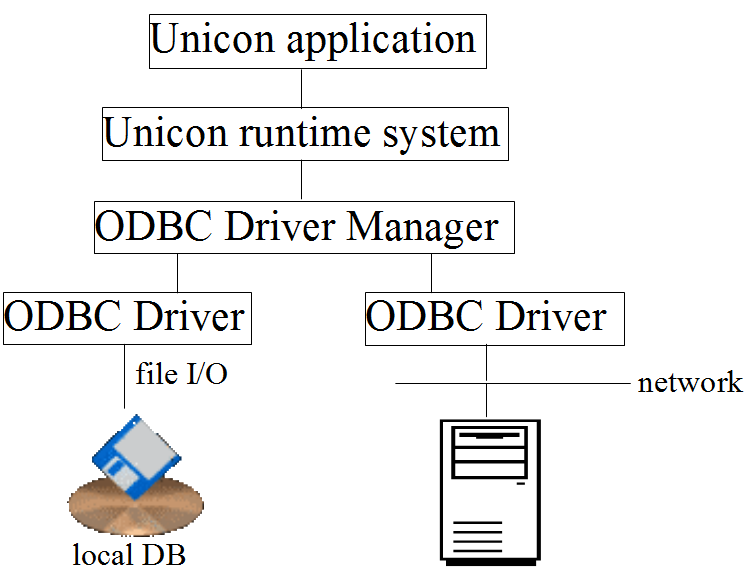
\includegraphics[width=3.2in,height=2.4in]{ub-img/odbcarch.png}
\end{center}

{\sffamily\bfseries Figure 6-1:}
{\sffamily Unicon and ODBC hide underlying architecture from
 applications}

\bigskip

To use Unicon's SQL facilities, you must have several
software components in place. First, you need a SQL server that
supports ODBC. You can buy a commercial SQL server, or
use a free server such as \index{MySQL}MySQL
(\texttt{www.mysql.com}) or \index{PostgreSQL}PostgreSQL
(\texttt{www.postgresql.org}).

Second, you need an account, password, and permissions on the SQL
server in order to connect to it. The details are
server-dependent and outside the scope of this book.

Third, your client machine needs an \index{driver manager!ODBC}ODBC
driver manager, and an ODBC driver for your SQL server; these must
be configured properly. The driver manager is a component
that connects applications to various databases; ODBC
drivers are dynamic link libraries that database vendors supply
to talk to their database.  Figure 6-2 shows database configuration
for MySQL via the MyODBC GUI dialog box on Windows (left), and in a
{\raise.17ex\hbox{$\scriptstyle\sim$}}/odbc.ini file on Linux (right).
In both cases, configuration involves knowing the internet server
name or IP address, the port, and the database to connect to. For that
triplet, you get to define a name called a DSN or data source name,
which is the name that Unicon will pass in to \texttt{open()}. In the
Windows dialog, this name is a textfield explicitly named as a DSN,
while in the Linux odbc.ini file, it is at the top, inside the square
brackets.

In both cases, there are a lot of additional options which are beyond
the scope of this book.  On Windows, each ODBC driver may have its own
custom dialogs for configuration, while on Linux the odbc.ini file is
more the property of the driver manager and is used to configure all
the various drivers. As a fair warning, the details required in the
dialogs or the exact syntax of the odbc.ini and its required entries
for a given driver change slightly from time to time and are beyond
the scope of this book.  Consult current ODBC documentation for the
driver manager on your platform and the specific database to which
you are connecting.

\bigskip

\noindent
\begin{tabular}{@{}c@{}}{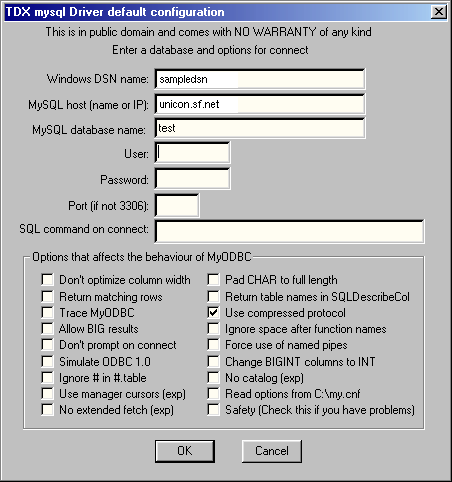
\includegraphics[width=3.8in,height=4.0in]{ub-img/odbcconf.png}}\end{tabular}
\hspace*{.04in}
\begin{tabular}{@{}c@{}}
\begin{tabular}{l}
\texttt{[phones]}\\
\texttt{Driver = /usr/lib64/libmyodbc5.so}\\
\texttt{Description = phone example}\\
\texttt{Server = localhost}\\
\texttt{Database = phonebook}\\
\texttt{Port = 3306}
\end{tabular}
\end{tabular}

{\sffamily\bfseries Figure 6-2:}
{\sffamily Configuring ODBC on Windows (left) and Linux (right)}

\bigskip


Once you have the ODBC software set up,
writing the Unicon client program to connect to your database is
straightforward.

\subsection*{Opening a SQL database}

To connect to a SQL database, call \texttt{open()}
with mode \texttt{"o"}. This establishes a
session with a data source. The filename argument to \texttt{open()} is
the data source to which you are connecting; it is associated with a
particular ODBC driver, remote database server machine or IP number,
and port within the ODBC driver manager. Mode \texttt{"o"} is followed
by additional string arguments to \texttt{open()}. The first is an optional
default table name used in the various functions that take a table
name. Generally the arguments must then include the user name and
password to use in
connecting to the specified data source. Here is an example that
establishes a connection to a database:

\iconcode{
f := open("unicondb", "o", "scott", "tiger")}

The \texttt{open()} function returns a value that supports many of the
operations of both a file and a table, or fails if the connection
cannot be established. The underlying session information is shared by
multiple calls to \texttt{open()} the same database. In addition to
the network connection and SQL session information that is retained,
each database file value maintains a current \textit{selection}
consisting of a set of rows corresponding to the current query, and a
\textit{cursor position} within that selection. When a database is
first opened, the selection consists of a null set containing no rows
and no columns.

\subsection*{Querying and modifying a SQL database}

Subsequent queries to the database can be made by calling
\texttt{sql(db, sqlcmd)}. The \index{sql()}\texttt{sql()} function sets
the current selection within the database and places the cursor at the
beginning of the set of selected rows. For example, to obtain Vic
T's phone number you might say

\iconcode{
sql(f, "select phone from addresses where
name='Vic T'")}

Vic's phone number is included if you use the original
\texttt{select *} query, but the more specific your query, the less
time and network bandwidth is wasted sending data that your client
application must filter out. You should do as much work on the server
(in SQL) as possible to make the client more efficient.

Since the function \texttt{sql()} transmits arbitrary SQL statements to
the server, it can be used for many operations besides changing the
current selection. The \texttt{sql()} function returns a null value
when there is no return value from the operation, such as a
\texttt{create table} statement. Its return value can be of varying
type for other kinds of queries, and it can fail, for example if the
SQL string is malformed or requests an impossible operation.

\subsection*{Traversing the selected rows}

To walk through the rows of your current database selection, you call
\index{fetch()!SQL}\texttt{fetch(db)}. The value returned is a
\textit{row} that has many of the operations of a record or a table,
namely field access and subscripting operators. For example, if
\texttt{fetch(db)} returns a row containing columns Name, Address, and
Phone, you can write

\iconcode{
row := fetch(db) \\
write(row.Name) \\
write(row["Address"])
}

\noindent
Called with one argument, \texttt{fetch(db)} advances the cursor
one position. With two arguments, \texttt{fetch(db, col)} produces a
column from the current row without advancing the cursor.

\subsection*{A SQL example application}

\index{SQL}A human resources database might include two tables. One
table might maintain employee information, such as names,
identification numbers, and phone numbers, while another table
maintains entries about specific jobs held, including
employee's ID, the pay rate, a code indicating whether
pay is hourly or salaried, and the job title. Note that the SQL is
embedded within a string literal.

\iconcode{
sql(db, "create table employees (id varchar(11), name
varchar(40),\\
\>\>\>\> phone varchar(15))") \\
sql(db, "create table jobs (id varchar(11), payrate
integer, is\_salaried char,\\
\>\>\>\> title varchar(40))")
}

\noindent
Inserting rows into the database looks like

\iconcode{
sql("insert into employees (id, name, phone) values(32,
'Ray',
'274-2977')")}

Now, how can you print out the job title for any particular employee? If
you have the employee's identification number, the
task is easy, but let's say you just have their name.
These are the kinds of jobs for which SQL was created. Information from
the employees table is effortlessly cross-referenced with the jobs
table by the following SQL. The string is long so it is split into
two lines. A Unicon string literal spans multiple lines when the
closing doublequote has not been found and the line ends with an
underscore character.

\iconcode{
sql(db, "select name,title from employees,jobs \_ \\
\>   \ \ \ \ \ \ where name='Ray' and
employees.id = jobs.id") \\
while write(fetch(db).Title)
}

\subsection*{SQL types and Unicon types}

SQL has many data types, most of which correspond to Unicon types.
\texttt{CHAR} and \texttt{VARCHAR} correspond to Icon
strings; \texttt{INTEGER} and \texttt{SMALLINT} correspond to integers;
\texttt{FLOAT} and \texttt{REAL} correspond to reals, and so on. The
philosophy is to convert between Icon and SQL seamlessly and with
minimal changes to the data format, but you should be aware that these
are not exact matches. For example, it is possible to define a
\texttt{FLOAT} with more precision than an Icon real, and it is easy to
produce an Icon string that is longer than the maximum allowed
\texttt{VARCHAR} size on most SQL servers. Unicon programmers writing
SQL clients must be aware of the limitations of the SQL implementations
they use.

Unicon has structure types for which there is no SQL equivalent. Values
of these types cannot be inserted into a SQL database unless you
explicitly convert them to a SQL-compatible type (usually a string)
using a function such as \texttt{xencode()}.
SQL also has types not found in Unicon such as bit
strings, timestamps, and BLOBS; they are represented
by strings, and strings are used to insert such values into SQL
databases. Strings are also used to represent out-of-range values when
reading SQL columns into Unicon.

\subsection*{More SQL database functions}

SQL databases are feature-rich enough to warrant a suite
of functions in addition to those they
share with other kinds of files and databases. These functions are
described in detail in Appendix A, but some of them deserve special
mention. The function \texttt{dbtables(db)} is useful to obtain a
listing of the data sources available within a particular database.
Function \texttt{dbcolumns(db)} provides detailed information about the
current table that is useful in writing general tools for viewing or
modifying arbitrary SQL databases.

The functions \texttt{dbproduct(db)} and \texttt{dbdriver(db)} produce
information about the DBMS on which \texttt{db} resides, and the
\index{ODBC}ODBC driver software used in the connection.
The function \texttt{dblimits(db)} produces the upper bounds for many
DBMS system parameters, such as the maximum number of columns allowed
in a table. These functions return their results as
a record or list of records whose field names and descriptions
are given in Appendix A.

\section{Tips and Tricks for SQL Database Applications}

In addition to the complexity of learning SQL itself, SQL database
applications have a characteristic flavor which may or may not seem
natural to the Unicon programmer.

\subsection*{Operating on large files}

Asking for 200MB of data in a remote SQL database is a good way to
bring a computer to its knees. Some SQL operations are slow due to an
inefficient query on the remote server, while others are slow because
large amounts of data are transmitted over a limited network
connection. For a fixed amount of data, operation time will vary
radically depending on how it is organized; fewer, larger tuples are
transmitted faster than many smaller tuples.

\subsection*{Use multiple connections to nest queries}

It is common to use more than one table at once. Some times this is
using SQL's \texttt{JOIN} operation, but sometimes it
is not. If you try to nest a second query inside a first one, you will
quickly find that on a given connection, only one \texttt{SELECT} and
one row set is maintained at a time. The second \texttt{SELECT}
replaces the first, so for example:

\iconcode{
db := open("mydsn",
"o", ...) \\
sql(db, {\textquotedblleft}SELECT ...{\textquotedblright}) \\
while r := fetch(db) do \{ \\
\>   sql(db, {\textquotedblleft}SELECT ...{\textquotedblright}) \\
\>   while r2 := fetch(db) do write(r2.foo) \\
\>   \}
}

\noindent
does not work. Within your operating system and database
server's limits, the easy solution is to open multiple
connections to your database:

\iconcode{
db1 := open("mydsn",
"o", ...) \\
db2 := open("mydsn",
"o", ...) \\
sql(db, {\textquotedblleft}SELECT ...{\textquotedblright}) \\
while r := fetch(db) do \{ \\
\>   sql(db2, {\textquotedblleft}SELECT ...{\textquotedblright}) \\
\>   while r2 := fetch(db2) do write(r2.foo) \\
\>   \}
}

\subsection*{Dynamic records}

Rows are represented as a special kind of Unicon record whose
fields are determined at run-time from the names
of selected columns. Record types introduced at runtime
are called \textit{dynamic records}, and they are useful in other
contexts besides databases.

The function \index{constructor!dynamic record
type}\texttt{constructor(rname, field, field, ...)} produces a
procedure that constructs records named
\texttt{rname} with the given fields. The field names
can be arbitrary strings, but only legal identifiers
will be subsequently accessible via the field operator (\texttt{.})

\subsection*{The \texttt{db} library}

The declaration \texttt{link db} provides simplified SQL access routines
for non-SQL programmers.
This library will not allow you to avoid learning SQL for long,
but may ease the conversion from Unicon structure values into SQL
strings for transmission over the network.
The most useful of these procedures is \texttt{dbupdate()}, which sends
a record (tuple) to the database. The following example updates two
columns within a row returned by \texttt{fetch()}.

\iconcode{
row := fetch(db) \\
row.Name := "Bill Snyder" \\
row["Address"] := "6900 Tropicana Blvd" \\
dbupdate(db, row)
}

Of course, before a fetch can be performed, a row set must have been
selected. The procedure \texttt{dbselect(db, columns, filter, order)}
selects tuples containing columns from the database, with optional
filter(s) and ordering rule(s).
Inserting and deleting rows is performed by procedures
\texttt{dbinsert()} and \texttt{dbdelete()}. The \texttt{dbinsert()}
function takes two parameters for each column being inserted, the
column name and then the value.

\subsection*{Unwritable tuples}

Many SQL selections are read-only.  The relational combination of
columns from different tables is powerful, but the resulting
selections are non-updatable.  Another example of a read-only query is
a \texttt{GROUP BY} query, which is usually applied before an
aggregate count. Executing a \texttt{SELECT *} on a single table is
updatable, but if you do something fancier, you will have to know the
semantics of SQL to tell whether the result may be modified.

\section{Summary}

Databases are a standard form of persistent storage for modern
applications. The notation for manipulating a database looks like
a sequence of table and record operations, comprising a
combination of Unicon and SQL statements. Database
facilities give programmers direct access and control over the
information flow to and from permanent storage.


\clearpage\section{Chapter 7: Graphics}

Unicon provides a rich high level interface to 2D and 3D raster
graphics, text fonts, colors, and mouse input facilities provided by an
underlying system, such as the X Window System.
Unicon{\textquotesingle}s graphics are portable across multiple
platforms. The most important characteristics of the graphics
facilities are:

\begin{itemize}\itemsep0pt
\item Simplicity, ease of learning
\item Windows are integrated with Unicon{\textquotesingle}s existing I/O
functions
\item Straightforward input event model
\end{itemize}
This chapter presents Unicon's 2D and 3D graphics facilities.
Some material on 2D graphics
comes from University of Arizona CS TR93-9. The 3D graphics sections
come from Unicon TR 9, whose original author is Naomi Martinez. The
definitive reference for the 2D
graphics facilities is {\textquotedbl}Graphics Programming in
Icon{\textquotedbl} by Griswold, Jeffery, and Townsend, and this book
is of value for writing 3D programs. Online references
for the graphics facilities also come with the software distributions.

Because different platforms have radically different capabilities, there
is a trade-off between simplicity, portability, and full access to the
underlying machine. Unicon aims for simplicity and ease of programming
rather than full low-level access.

\subsection{2D Graphics}

Unicon{\textquotesingle}s 2D facilities provide access to graphics
displays without enforcing a particular user interface look-and-feel.
Events other than keystrokes and mouse events are handled automatically
by the runtime system. Chapter 17 describes the standard class library
and user interface builder for Unicon applications.

Graphic interfaces are \index{event driven}\textit{event driven}; an
event reading loop is the control mechanism driving the application.
For example, if an application must be ready to redraw the contents
of its window at all times, it may not compute for long periods without
checking for window events. This event driven paradigm used in the
underlying implementation is optional at the Unicon application
level. Since Unicon windows handle many events automatically and
{\textquotedbl}take care of themselves{\textquotedbl}, applications
follow the event driven paradigm only when it is needed.
Unicon{\textquotesingle}s extensive
use of default values make simple graphics applications extremely easy
to program, while providing flexibility where it is needed in more
sophisticated applications.

\subsubsection{Window Basics}

A window is a special file opened with mode
\texttt{{\textquotedbl}g{\textquotedbl},} appearing on-screen as a
rectangular space for text and/or graphics. Windows support text I/O,
much as one uses a text terminal. A simple
Unicon graphics program might look like this:

\iconcode{
\ \ \ procedure main()\\
 \ \ \ \ \ w := open({\textquotedbl}hello{\textquotedbl},
{\textquotedbl}g{\textquotedbl})\\
 \ \ \ \ \ write(w, {\textquotedbl}hello, world{\textquotedbl})\\
 \ \ \ \ \ \# do processing ... use w as if it were a terminal\\
 \ \ \ \ \ close(w)\\
 \ \ end
}

Windows are open for both reading and writing, and support the usual
file operations with the exceptions of \texttt{seek()} and
\texttt{where()}. Unlike regular files, the \texttt{type()} of a
window is {\textquotedbl}window{\textquotedbl}. Like other files,
windows close automatically when the program terminates, so the call to
\texttt{close()} in the above example is optional.

Bit-mapped, or raster, graphics constitute a second programming model
for windows. There are no programming
{\textquotedbl}modes{\textquotedbl} and code that uses graphics may be
freely intermixed with code that performs text operations. There are
many graphics functions and library procedures, detailed in Appendices
A and B.

\paragraph{\&window: the Default Window Argument}

The keyword \texttt{\&window} is a default window for graphics.
\texttt{\&window} starts with a null value; only window values
(and \texttt{\&null}) may
be assigned to \texttt{\&window}. \texttt{\&window} is a default
argument to most graphics functions and is used implicitly by various
operations. If a program uses \texttt{\&window}, the argument can be
omitted from calls to functions such as \texttt{EraseArea()} and
\texttt{WAttrib()}. The window argument is required for calls to file
functions such as \texttt{write()} and \texttt{writes()} since these
functions default to \texttt{\&output}, not \texttt{\&window}. The
default window shortens the code for graphics-oriented programs and
makes it faster.

\paragraph{2D Graphics Coordinates}

The 2D graphics functions use an integer coordinate system based on
pixels (picture elements). Like the text coordinate system, 2D
graphics coordinates start in the upper-left corner of the screen.
From that corner the positive x direction lies to the right and the
positive y direction moves down. Unlike text coordinates, the
graphics coordinate axes are zero-based, which is to say that the very
top leftmost pixel is (0,0) by default.

Angles are real numbers given in radians, clockwise starting at the 3
o{\textquotesingle}clock position. Many functions operate on
rectangular regions specified by x, y, width, and height components.
Width and height may be negative to extend the rectangle
left or up from x and y. Screen output may be limited to a
rectangle within the window called the clipping region. The
clipping region is set or unset using the function \texttt{Clip()}.

\paragraph{Window Attributes}
A window{\textquotesingle}s state has many \textit{attributes}
with associated values. Some values are defined by the system, while
others are under program control, with reasonable defaults. When
opening a window, \texttt{open()} allows string arguments after the filename
and mode that specify initial values of
attributes when the window is created. For example, to say hello in
italics on a blue background one may write:

\iconcode{
\ \ \ procedure main()\\
 \ \ \ \ \ w := open({\textquotedbl}hello{\textquotedbl},
{\textquotedbl}g{\textquotedbl},
{\textquotedbl}font=sans,italics{\textquotedbl},
{\textquotedbl}bg=blue{\textquotedbl})\\
 \ \ \ \ \ write(w, {\textquotedbl}hello, world{\textquotedbl})\\
 \ \ \ \ \ \# processing ...\\
 \ \ end}

After a window is created, its attributes are read and set using
the function \texttt{WAttrib(w,s1,s2,...)}. Arguments to
\texttt{WAttrib()} that have an equals sign are assignments that set
the given value if possible; \texttt{WAttrib()} fails otherwise.
\texttt{open()} only allows such attribute assignments. Some
attributes can only be read by \texttt{WAttrib()} and not set.

String arguments to \texttt{WAttrib()} that have an attribute name but
no value are queries which return the attribute value.
\texttt{WAttrib()} generates a string result for each argument; a query
on a single argument produces just the value of that attribute; for
multiple arguments and in the case of assignment, the result is the
\texttt{\textit{attr}}\texttt{=}\texttt{\textit{val}} form attribute
assignments take. Attributes are also frequently set implicitly by
the user{\textquotesingle}s manipulation of the window; for instance,
cursor or mouse location or window size.

The following attributes are maintained on a per-window basis.
Attribute values are string encodings. Usage refers to whether the
attribute may be read, written or both. RWO and WO attributes can be
assigned only when the window is opened.

\bigskip

{\centering\sffamily\bfseries
Table 7-1

Canvas Attributes
}

\begin{center}
\tablehead{\hline
\centering \bfseries\itshape Name &
\centering \bfseries\itshape Type / Example &
\centering \bfseries\itshape Description &
\centering\arraybslash \bfseries\itshape Usage\\\hline}
\begin{supertabular}{|m{0.9622598in}|m{2.0323598in}|m{2.1712599in}|m{0.44835988in}|}
size &
pixel pair &
Size of window &
RW\\\hline
pos &
pixel pair &
Position of window on screen &
RW\\\hline
canvas &
normal, hidden &
Canvas state &
RW\\\hline
windowlabel &
string &
Window label (title) &
RW\\\hline
inputmask &
string &
select categories of input events &
RW\\\hline
pointer &
arrow, clock &
Pointer (mouse) shape  &
RW\\\hline
pointerx, pointery &
pixel &
Pointer (mouse) location  &
RW\\\hline
display &
device /
{\textquotedbl}my.cs.esu.edu:0{\textquotedbl}
&
(X11) device window resides on &
RWO\\\hline
depth &
\# of bits &
Display depth &
R\\\hline
displaywidth, displayheight &
pixel &
Display size &
R\\\hline
image &
string &
Initial window contents &
WO\\\hline
\end{supertabular}
\end{center}
Although all attribute values are encoded as strings, they represent
a range of window system features. The attribute \texttt{pointer} refers to
mouse pointer shapes that may be changed by the application during
different operations. The attribute \texttt{pos} refers to the position
of the upper-left corner of the window on the screen. Screen position
is specified by a string containing x,y coordinates,
e.g. \texttt{{\textquotedbl}pos=200,200{\textquotedbl}}.

\subsubsection{Graphics Contexts}

Some attributes are associated with the window itself, while others are
associated with the \textit{graphics context}, a set of resources
used by operations that write to windows. This distinction is unimportant
in simple applications but is useful in more sophisticated
applications that use multiple windows or draw many kinds of things in
windows. A graphics context has colors, patterns, line
styles, and text fonts and sizes.

Although they are called graphics contexts, text operations use these
attributes. Text is written using the foreground and background
colors and font defined in the graphics context. Table 7-2 lists
the attributes associated with a graphics context.

{\centering\sffamily\bfseries
Table 7-2
\par}

{\centering\sffamily\bfseries
Context Attributes
\par}

\begin{center}
\tablehead{\hline
\centering \bfseries\itshape Name &
\centering \bfseries\itshape Type / Example &
\centering \bfseries\itshape Description : Default &
\centering\arraybslash \bfseries\itshape Usage\\\hline}
\begin{supertabular}{|m{1.0163599in}|m{1.6261599in}|m{2.5233598in}|m{0.44835988in}|}
fg &
color \ / {\textquotedbl}red{\textquotedbl} &
Foreground color : black &
RW\\\hline
bg &
color \ / {\textquotedbl}0,0,0{\textquotedbl} &
Background color : white &
RW\\\hline
font &
font name &
Text font : fixed &
RW\\\hline
fheight, fwidth &
integer &
Text font max char height and width &
R\\\hline
leading &
integer &
Vertical \# pixels between text lines &
RW\\\hline
ascent, descent &
integer &
Font height above/below baseline &
R\\\hline
drawop &
logical op / reverse  &
Drawing operation: copy &
RW\\\hline
fillstyle &
stippled, opaquestippled &
Graphic fill style : solid &
RW\\\hline
pattern &
{\textquotedbl}4,\#5A5A{\textquotedbl} &
Fill pattern &
RW\\\hline
linestyle &
onoff, doubledash &
Drawing line style : solid  &
RW\\\hline
linewidth &
integer &
Drawing line width &
RW\\\hline
clipx, clipy, clipw, cliph &
integer &
Clip rectangle position and extent: 0 &
RW\\\hline
dx, dy &
integer &
Output coordinate translation : 0 &
R\\\hline
image &
string / {\textquotedbl}flag.xpm{\textquotedbl} &
Initial window contents &
WO\\\hline
\end{supertabular}
\end{center}
\paragraph{Binding Windows and Graphics Contexts Together}
Graphics contexts can be shared among windows, and multiple graphics
contexts can be used on the same window. An Unicon window value is a
\textit{binding} of a canvas (an area that may be drawn upon) and a
graphics context. A call
\texttt{open(s,{\textquotedbl}g{\textquotedbl})} creates both a canvas,
and a context, and binds them together, producing the binding as its
return value.

\texttt{Clone(w)} creates a binding of the canvas and attributes
of \texttt{w} with a new graphics context that is manipulated
independently. \texttt{Clone()} also accepts any number
of string attributes to apply to the new window value, as in
\texttt{open()} and \texttt{WAttrib()}.

After calling \texttt{Clone()}, two or more Unicon window values
write to the same canvas. The cursor location is stored in the
canvas, not the graphics context. Writing to the windows produces
concatenated (rather than overlapping) output. Closing one of the
window values removes the canvas from the screen but does not destroy
its contents; the remaining binding references an invisible pixmap.
The canvas is destroyed after the last binding associated with it
closes. Use of \texttt{Clone()} can significantly enhance performance
for applications that require frequent graphics context manipulations.

\paragraph{Subwindows}
The function \texttt{Clone()} can also be used to create subwindows,
which are canvases that reside within other windows.
\ \texttt{Clone(w, {\textquotedblleft}g{\textquotedblright}, ...)}
opens a 2D subwindow within \texttt{w}, and \texttt{Clone(w,
{\textquotedblleft}gl{\textquotedblright}, ...)} opens a 3D subwindow
within \texttt{w}. Applications must supply position and size
attributes when they create a subwindow. Input events
to a subwindow are not seen on the enclosing parent window and vice
versa; both windows must be polled or supplied to \texttt{WActive()} or
\texttt{select()} in order to handle input.

\paragraph{Coordinate Translation}
In 2D, context attributes \texttt{dx} and \texttt{dy} perform output
coordinate translation. \texttt{dx} and \texttt{dy} take integer values
and default to zero. These integers are added into the coordinates of
all output operations that use the context; input coordinates in
\texttt{\&x} and \texttt{\&y} are not translated.

\subsubsection{Events}

User input such as keystrokes and mouse clicks are called
\textit{events}. Many events are handled by Unicon automatically,
including window redrawing and resizing, etc.
Other events are put on a queue in the order they occur, for
processing by the Unicon program. When reading from a window using file
input functions such as \texttt{reads(w, 1)}, only keyboard events are
produced; mouse and other events are dropped.

The primary input function for windows is \texttt{Event(w),} which
produces the next event for window \texttt{w} and removes it from the
queue. If the event queue is empty, \texttt{Event()} waits for an
event. Keyboard events are returned as strings, while mouse events are
returned as integers. Special keys, such as function and arrow keys,
are also returned as integers, described below. \texttt{Event()} also
removes the next two elements and assigns the keywords \texttt{\&x} and
\texttt{\&y} the pixel coordinates of the mouse at the time of the
event. The values of \texttt{\&x}, \texttt{\&y} remain available until
a subsequent call to \texttt{Event()} again assigns to them.
\texttt{Event()} sets the keyword \texttt{\&interval} to the number of
milliseconds that have elapsed since the last event (or to zero for the
first event). Keywords \texttt{\&control}, \texttt{\&shift}, and
\texttt{\&meta} are set by \texttt{Event()} to return the null value if
those modifier keys were pressed at the time of the event; otherwise
they fail. For resize events, \texttt{\&interval} is set to zero and
modifier keywords fail. Keywords associated with event processing on
windows are summarized in Table 7-3:

{\centering\sffamily\bfseries
Table 7-3

Window Input Event Keywords
}

\begin{center}
\tablehead{\hline
\centering \bfseries\itshape Keyword &
\centering\arraybslash \bfseries\itshape Description\\\hline}
\begin{supertabular}{|m{0.91775984in}|m{2.3525598in}|}
\texttt{\&x} &
Mouse location, horizontal\\\hline
\texttt{\&y} &
Mouse location, vertical\\\hline
\texttt{\&row} &
Mouse location, text row\\\hline
\texttt{\&col} &
Mouse location, text column\\\hline
\texttt{\&interval} &
Time since last event, milliseconds\\\hline
\texttt{\&control} &
Succeeds of Control key pressed\\\hline
\texttt{\&shift} &
Succceds if Shift key pressed\\\hline
\texttt{\&meta} &
Succeeds if Alt (meta) key pressed\\\hline
\end{supertabular}
\end{center}
\paragraph{Keyboard Events}
The regular keys that Unicon returns as one-letter strings correspond
approximately to the lower 128 characters of the ASCII character set.
These characters include the control keys, the escape key, and the
delete key. Modern keyboards have many additional keys, such as
function keys, arrow keys, {\textquotedbl}page down{\textquotedbl},
etc. Unicon produces integer events for these special keys. A
collection of symbol definitions for special keys is available in the
library include file \texttt{keysyms.icn}. The most common
of these are \texttt{Key\_Down}, \texttt{Key\_Up}, \texttt{Key\_Left},
\texttt{Key\_Right}, \texttt{Key\_Home}, \texttt{Key\_End},
\texttt{Key\_PgUp}, \texttt{Key\_PgDn}, \texttt{Key\_F1...Key\_F12},
and \texttt{Key\_Insert}.

\paragraph{Mouse Events}
Mouse events are returned from \texttt{Event()} as integers indicating
the type of event, the button involved, etc. Keywords allow the
programmer to treat mouse events symbolically. The event keywords are:

{\centering\sffamily\bfseries
Table 7-4
\par}

{\centering\sffamily\bfseries
Window Input Event Codes
\par}

\begin{center}
\tablehead{\hline
\centering \bfseries\itshape Keyword &
\centering\arraybslash \bfseries\itshape Event\\\hline}
\begin{supertabular}{|m{0.9247598in}|m{2.3525598in}|}
\texttt{\&lpress} &
Mouse press left\\\hline
\texttt{\&mpress} &
Mouse press middle\\\hline
\texttt{\&rpress} &
Mouse press right\\\hline
\texttt{\&lrelease} &
Mouse release left\\\hline
\texttt{\&mrelease} &
Mouse release middle\\\hline
\texttt{\&rrelease} &
Mouse release right \\\hline
\texttt{\&ldrag} &
Mouse drag left \\\hline
\texttt{\&mdrag} &
Mouse drag middle \\\hline
\texttt{\&rdrag} &
Mouse drag right \\\hline
\texttt{\&resize} &
Window was resized \\\hline
\end{supertabular}
\end{center}
The following program uses mouse events to draw a box that follows the
mouse pointer around the screen when a mouse button is pressed. The
attribute \texttt{drawop=reverse} allows drawing operations to serve as
their own inverse; see [Griswold98] for more about the \texttt{drawop}
attribute. Function \texttt{FillRectangle()} draws a filled rectangle
on the window and is described in the reference section. Each time
through the loop the program erases the box at its old location and
redraws it at its new location; the first time through the loop there
is no box to erase so the first call to \texttt{FillRectangle()} is
forced to fail by means of Unicon{\textquotesingle}s
\texttt{{\textbackslash}} operator.

\iconcode{
procedure main()\\
 \ \ \&window := open({\textquotedbl}hello{\textquotedbl},
{\textquotedbl}g{\textquotedbl},
{\textquotedbl}drawop=reverse{\textquotedbl})\\
 \ \ repeat if Event() === (\&ldrag {\textbar} \&mdrag {\textbar}
\&rdrag) then \{\\
 \ \ \ \ \ \# erase box at old position, then draw at new
position\\
 \ \ \ \ \ FillRectangle({\textbackslash}x, {\textbackslash}y, 10,
10)\\
 \ \ \ \ \ FillRectangle(x := \&x, y := \&y, 10, 10)\\
 \ \ \ \ \ \}\\
end}

The program can inspect the window{\textquotesingle}s
state using \texttt{WAttrib()}. Between the time the mouse event
occurs and the time it is produced by \texttt{Event()}, the mouse may
have moved. In order to get the current mouse location, use
\texttt{QueryPointer()} (see below).

When more than one button is depressed as the drag occurs, drag events
are reported on the most recently pressed button. This behavior is
invariant over all combinations of presses and releases of all three buttons.

Resize events are reported in the same format as mouse events.
In addition to the event code, \texttt{\&x}, \texttt{\&y}, \texttt{\&col} and
\texttt{\&row} are assigned integers that indicate the window{\textquotesingle}s
new width and height in pixels and in text columns and rows,
respectively. Resize events are produced when the window manager
(usually at the behest of the user) resizes the window; no event is
generated when an Unicon program resizes its window.

\paragraph{Key Release, Mouse Motion, and Window Closure Events}
The canvas attribute \texttt{inputmask} allows programs to request three kinds
of additional input events on windows. These events pose enough
performance or portability obstacles that they are not produced by
default. An {\textquotedblleft}m{\textquotedblright} in the inputmask
requests mouse motion events even when no mouse button is depressed; by default only
{\textquotedblleft}drag{\textquotedblright} events are reported. If the
inputmask contains a {\textquotedblleft}k{\textquotedblright}, events
will be generated when keyboard keys are released. An inputmask
attribute containing a {\textquotedblleft}c{\textquotedblright}
requests an event when a window closure is externally triggered,
as in the case when a titlebar
{\textquotedblleft}x{\textquotedblright} button is pressed.

\paragraph{Event Queue Manipulation}
The event queue is an Unicon list that stores events until the program
processes them. When a user presses a key, clicks or drags a mouse,
or resizes a window, three values are placed on the event queue: the
event itself, followed by two integers containing associated event
information.

\texttt{Pending(w)} produces the event queue for window \texttt{w}.
If no events are pending, the list is empty. The list returned by
\texttt{Pending()} is
attached to the window. Additional events may be added to it at any
time during program execution. It is an ordinary list and
can be manipulated using Unicon{\textquotesingle}s list functions and
operators.

When several windows are open, the program may need to wait for activity on
any of the windows. Each pending list could be checked until a nonempty list is
found, but such a busy-waiting solution is wasteful of CPU time. The
function \texttt{Active()} waits for window activity, relinquishing the CPU
until an event is pending on one of the open windows, and then returns
a window with a pending event. A window is said to starve if its
pending events are never serviced. \texttt{Active()} cycles through open
windows on repeated calls in a way that avoids window starvation.

\subsubsection{Colors}

Unicon recognizes a set of string color names based loosely on a color
naming system found in [Berk82]. The color names consist of simple
English phrases that specify hue, lightness, and saturation values of
the desired color. The syntax of colors is

[\textit{lightness}] [\textit{saturation}] [\textit{hue}[ish]]
\textit{hue}

where lightness is one of pale, light, medium, dark, or deep; saturation
is one of weak, moderate, strong, or vivid; and where hue is any of
black, gray, grey, white, pink, violet, brown, red, orange, yellow,
green, cyan, blue, purple, or magenta. A single space or hyphen
separates each word from its neighbor. When two hues are supplied
(and the first hue has no \texttt{ish} suffix), the resulting hue is
halfway in between the two named hues. When a hue with an \texttt{ish} suffix
precedes a hue, the resulting hue is three-fourths of the way
from the \texttt{ish} hue to the main hue. When adding \texttt{ish} to a word
ending in e, the e is dropped (for example, purple becomes purplish); the ish
form of red is reddish. Mixing radically different colors such as
yellow and purple does not usually produce the expected results. The
default lightness is \texttt{medium} and the default saturation is
\texttt{vivid}. Note that human perception of color varies significantly, as
do the actual colors produced from these names on different monitors.

\paragraph{Color Coordinate Systems and Gamma Correction}
In addition to the standard color names, platform-specific color names
may be supported. Colors may also be specified by strings encoding the
red, green, and blue components of the desired color. Unicon accepts
the hex formats {\textquotedbl}\#rgb{\textquotedbl} in which r, g, and
b are 1 to 4 hex digits each. Red, green, and blue may also be given
in decimal format, separated by commas. The components are given on a
linear scale from 0 to 65535, although displays typically offer far
less precision and nonlinear colors. For example,
{\textquotedbl}bg=32767,0,0{\textquotedbl} requests a medium red
background; if the display is incapable of such, it approximates it as
closely as possible from the available colors.
{\textquotedbl}fg=0,65000,0{\textquotedbl} requests a vivid green
foreground. If colors appear darker than they should, the window system
is not providing linear colors. Unicon can be told to perform the
correction by means of the gamma attribute; 1.0 is a default (no gamma
correction), and experimenting with values between 2 and 3 usually
provides satisfactory results.

\subsubsection{Fonts}

Fonts are specified by a comma-separated string of up to four fields
supplying the font{\textquotesingle}s family name, followed by optional
size or italic or bold designations in any order. The fonts available
vary widely from system to system. Four font family names available on
all Unicon systems include serif, sans, typewriter, and mono. These
families map onto the system{\textquotesingle}s closest approximation
of Times, Helvetica, Courier, and a monospaced console font. Font sizes
are given in pixel height.

\subsubsection{Images and Palettes}

\texttt{DrawImage(x, y, s)} draws a rectangular area using an image string.
String \texttt{s} has the form
{\textquotedbl}\textit{width},\textit{palette},\textit{data}{\textquotedbl}.
\textit{width} is the width of the rectangle drawn, \texttt{palette} is a code
that defines the colors corresponding to data values, and the rest of
the data supplies pixel values. Predefined palettes and palette
functions help to provide this capability. Image and palette
functions are described fully in [Griswold98].

\subsubsection{Patterns}

The context attribute \texttt{fillstyle} determines the
pixels used by draw and fill functions like \texttt{FillPolygon()}.
If the \texttt{fillstyle} is not \texttt{solid}, a pattern in
the filled area is drawn in the foreground color; other pixels are
drawn in the background color
({\textquotedbl}fillstyle=textured{\textquotedbl}). Patterns are
specified by the function Pattern(w,s), which associates a pattern
denoted by s with w{\textquotesingle}s context. String s is either
the name of a standard pattern, or a representation of the bits that
define the pattern. Pattern representations are of the form
{\textquotedbl}width,\#bits{\textquotedbl} where 1 {\textless}= width
{\textless}= 32. The window system may define a limit as low as 8 on
the pattern{\textquotesingle}s width and height.

The height of the pattern is defined by the number of rows in the bits
component of the pattern string. Bits consists of a series of
numbers, each supplying one row of the pattern, in hexadecimal format.
Each digit defines four bits and each row is defined by the number of
digits required to supply width bits. For example, the call

\iconcode{
\>   Pattern({\textquotedbl}4,\#5A5A{\textquotedbl})}

\noindent defines a 4x4 pattern where each row is defined by one hex digit.

\subsubsection{Pme: a Pixmap Editor}

A simple image editor called Pme, demonstrates event processing
including mouse events. Pme displays both a small and a
{\textquotedbl}magnified{\textquotedbl} display of the image being
edited, allows the user to set individual pixels, and allows the user
to save the image; it is well-suited for constructing and hand-editing
small images such as icons and textures for use in larger 2D or 3D
scenes. Pme consists of four procedures and employs several graphics
functions. A sample screen image of Pme is presented in Figure 7-1. The
{\textquotedblleft}real{\textquotedblright} image is in the upper left
corner; underneath it is a mouse icon which shows what color is drawn
by each of the mouse buttons.



\begin{center}
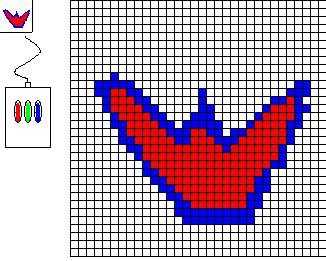
\includegraphics[width=1.7917in,height=1.3575in]{ub-img/ub-img11.jpg}
\end{center}

{\sffamily\bfseries Figure 7-1}
{\sffamily Pme editing a 32x32 image}

\bigskip

Pme starts by declaring and initializing several variables.

\bigskip

\iconcode{
link dialog \\
link file\_dlg \\
global lmargin, colors, colorbinds \\
procedure main(argv) \\
\>   local i := 1, j, s, e, x, y, width := 32, height := 32
}

The image width and height can be specified on the command line with a
{}-size option, for example, \ pme -size 16,64.

\iconcode{
\>   if argv[1]=={\textquotedbl}-size{\textquotedbl} then \{ \\
\>   \ \ \ i +:= 1 \\
\>   \ \ \ argv[2] ? \{ \\
\>   \ \ \ \ \ \ width := integer(tab(many(\&digits))) {\textbar}
stop({\textquotedbl}bad -size{\textquotedbl}) \\
\>   \ \ \ \ \ \ ={\textquotedbl},{\textquotedbl} {\textbar}
stop({\textquotedbl}bad -size{\textquotedbl}) \\
\>   \ \ \ \ \ \ height := integer(tab(0)) {\textbar}
stop({\textquotedbl}bad -size{\textquotedbl}) \\
\>   \ \ \ \ \ \ i +:= 1 \\
\>   \ \ \ \ \ \ \} \\
\>   \ \ \ \}
}

Following the size arguments, Pme checks for a filename specifying the
bitmap to edit. If one is found, it is read into the regular scale
image, and then the magnified scale image is constructed by reading
each pixel using the function \texttt{Pixel()}, and filling an 8x8
rectangle with the corresponding color.

\iconcode{
\>   \ \ \ i := j := 0 \\
\>   \ \ \ every p := Pixel(0, 0, width, height) do \{ \\
\>   \ \ \ \ \ \ Fg(p) \\
\>   \ \ \ \ \ \ FillRectangle(j * 8 + lmargin + 5, i * 8, 8, 8) \\
\>   \ \ \ \ \ \ j +:= 1 \\
\>   \ \ \ \ \ \ if j = width then \{ i +:= 1; j := 0 \} \\
\>   \ \ \ \ \ \ \}
}

After the images are loaded with their initial contents, if any, a grid
is drawn on the magnified image to delineate each individual
pixel{\textquotesingle}s boundary. The user{\textquotesingle}s mouse
actions within these boxes change the colors of corresponding pixels in
the image. An list of three bindings to the window, each with an
independently-set foreground color, is used to represent the color
settings of the mouse buttons.

\iconcode{
\>   colors :=
[Clone({\textquotedbl}fg=red{\textquotedbl}),Clone({\textquotedbl}fg=green{\textquotedbl}),Clone({\textquotedbl}fg=blue{\textquotedbl})]
}

The main event processing loop of Pme is simple: Each event is fetched
with a call to \texttt{Event()} and immediately passed into a case
expression. The keystroke \texttt{{\textquotedbl}q{\textquotedbl}}
exits the program; the keystroke
\texttt{{\textquotedbl}s{\textquotedbl}} saves the bitmap in a file by
calling \texttt{WriteImage()}, asking for a file name if one has not
yet been supplied.

\iconcode{
\>   \ \ \ case e := Event() of \{ \\
\>   \ \ \ {\textquotedbl}q{\textquotedbl}{\textbar}{\textquotedbl}{\textbackslash}e{\textquotedbl}:
return \\
\>   \ \ \ {\textquotedbl}s{\textquotedbl}{\textbar}{\textquotedbl}S{\textquotedbl}:
\{ \\
\>   \ \ \ \ \ \ if /s {\textbar} (e=={\textquotedbl}S{\textquotedbl})
then s := getfilename() \\
\>   \ \ \ \ \ \ write({\textquotedbl}saving image {\textquotedbl}, s,
{\textquotedbl} size {\textquotedbl},
width,{\textquotedbl},{\textquotedbl}, height) \\
\>   \ \ \ \ \ \ WriteImage( s, 0, 0, width, height) \\
\>   \ \ \ \ \ \ \}
}

Mouse events result in drawing a single pixel in both the magnified and
regular scale bitmaps using one of the colors depicted on the mouse icon. 

\iconcode{
\>   \ \ \ \&lpress {\textbar} \&ldrag {\textbar} \&mpress {\textbar}
\&mdrag {\textbar} \&rpress {\textbar} \&rdrag : \{ \\
\>   \ \ \ \ \ \ x := (\&x - lmargin - 5) / 8 \\
\>   \ \ \ \ \ \ y := \&y / 8 \\
\>   \ \ \ \ \ \ if (y {\textless} 0) {\textbar} (y {\textgreater}
height-1) {\textbar} (x {\textgreater} width) then next \\
\>   \ \ \ \ \ \ if x {\textgreater}= 0 then dot(x, y, (-e - 1) \% 3)
}

To change the color drawn by a mouse button, you click on it.

\iconcode{
\>   \ \ \ \ \ \ else \{ \# x {\textless} logical 0. User clicked in
mouse area \\
\>   \ \ \ \ \ \ \ \ \ if \&x {\textless} 21 then getacolor(1,
{\textquotedbl}left{\textquotedbl}) \\
\>   \ \ \ \ \ \ \ \ \ else if \&x {\textless} 31 then getacolor(2,
{\textquotedbl}middle{\textquotedbl}) \\
\>   \ \ \ \ \ \ \ \ \ else getacolor(3,
{\textquotedbl}right{\textquotedbl}) \\
\>   \ \ \ \ \ \ \ \ \ until Event() === (\&mrelease {\textbar}
\&lrelease{\textbar} \&rrelease) \\
\>   \ \ \ \ \ \ \ \ \ \} \\
\>   \ \ \ \ \ \ \}
}

Pixel drawing is handled by procedure \texttt{dot()}, whose third
argument specifies which button, and therefore which color to draw.
The dot is drawn using \texttt{FillRectangle()} in the magnified window; in
the regular scale window \texttt{DrawPoint()} suffices.

\iconcode{
procedure dot(x, y, c) \\
\>   if (x{\textbar}y) {\textless} 0 then fail \\
\>   FillRectangle(colors[c+1], x*8 + lmargin + 5, y*8, 8, 8) \\
\>   DrawPoint(colors[c+1], x, y) \\
\>   DrawRectangle(x*8 + lmargin + 5, y*8, 8, 8) \\
end
}

Pme illustrates several aspects of the Unicon graphics facilities. Note
the event-handling: a case expression handles various
keystrokes and mouse events with simpler control
structure than in most languages{\textquotesingle} GUI event processing.

\bigskip

{\sffamily\bfseries Listing 7-1}
{\sffamily\bfseries Pme: a Unicon bitmap editor}

\iconcode{
link dialog \\
link file\_dlg \\
global lmargin, colors \\
procedure main(argv) \\
\>   local i := 1, j, s, e, x, y, width := 32, height := 32 \\
\>   if argv[1]=={\textquotedbl}-size{\textquotedbl} then \{ \\
\>   \ \ \ i +:= 1 \\
\>   \ \ \ argv[2] ? \{ \\
\>   \ \ \ \ \ \ width := integer(tab(many(\&digits))) {\textbar}
stop({\textquotedbl}bad -size{\textquotedbl}) \\
\>   \ \ \ \ \ \ ={\textquotedbl},{\textquotedbl} {\textbar}
stop({\textquotedbl}bad -size{\textquotedbl}) \\
\>   \ \ \ \ \ \ height := integer(tab(0)) {\textbar}
stop({\textquotedbl}bad -size{\textquotedbl}) \\
\>   \ \ \ \ \ \ i +:= 1 \\
\>   \ \ \ \ \ \ \} \\
\>   \ \ \ \} \\
\>   lmargin := max(width, 65) \\
\>   if s := argv[i] then \{ \\
\>   \ \ \ \&window := open({\textquotedbl}pme{\textquotedbl},
{\textquotedbl}g{\textquotedbl},
{\textquotedbl}image={\textquotedbl}{\textbar}{\textbar}s) {\textbar}
stop({\textquotedbl}cannot open window{\textquotedbl}) \\
\>   \ \ \ width \ {\textless}:=
WAttrib({\textquotedbl}width{\textquotedbl}) \\
\>   \ \ \ height {\textless}:=
WAttrib({\textquotedbl}height{\textquotedbl}) \\
\>   \ \ \ lmargin := max(width, 65) \\
\>   \ \ \ WAttrib({\textquotedbl}size={\textquotedbl}{\textbar}{\textbar}(width*8+lmargin+5){\textbar}{\textbar}{\textquotedbl},{\textquotedbl}{\textbar}{\textbar}(height*8)) \\
\>   \ \ \ i := j := 0 \\
\>   \ \ \ every p := Pixel(0, 0, width, height) do \{ \\
\>   \ \ \ \ \ \ Fg(p) \\
\>   \ \ \ \ \ \ FillRectangle(j * 8 + lmargin + 5, i * 8, 8, 8) \\
\>   \ \ \ \ \ \ j +:= 1 \\
\>   \ \ \ \ \ \ if j = width then \{ i +:= 1; j := 0 \} \\
\>   \ \ \ \ \ \ \} \\
\>   \ \ \ \} \\
\>   else \{ \\
\>   \ \ \ \&window := open({\textquotedbl}pme{\textquotedbl},
{\textquotedbl}g{\textquotedbl},
{\textquotedblright}size={\textquotedblright} {\textbar}{\textbar}
(lmargin+width*8+5){\textbar}{\textbar}{\textquotedbl},{\textquotedbl}{\textbar}{\textbar}(height*8+5))
{\textbar} \\
 \ \ \ \ \ \ \ \ stop({\textquotedbl}cannot open window{\textquotedbl}) \\
\>   \ \ \ \} \\
\>   colors :=
[Clone({\textquotedbl}fg=red{\textquotedbl}),Clone({\textquotedbl}fg=green{\textquotedbl}),Clone({\textquotedbl}fg=blue{\textquotedbl})] \\
\>   every i := 1 to 3 do \{ \\
\>   \ \ \ DrawArc(4+i*10, height+68, 7, 22) \\
\>   \ \ \ FillArc(colors[i], 5+i*10, height+70, 5, 20) \\
\>   \ \ \ \} \\
\>   DrawRectangle( 5, height+55, 45, 60, 25, height+50, 5, 5) \\
\>   DrawCurve(27, height+50, 27, height+47, 15, height+39, \\
\>   \ \ \ \ \ \ \ \ \ \ 40, height+20, 25, height+5) \\
\>   Fg({\textquotedbl}black{\textquotedbl}) \\
\>   every i := 0 to height-1 do \\
\>   \ \ \ every j := 0 to width-1 do \\
\>   \ \ \ \ \ \ DrawRectangle(j*8+lmargin+5, i*8, 8, 8) \\
\>   DrawLine(0, height, width, height, width, 0) \\
\>   repeat \{ \\
\>   \ \ \ case e := Event() of \{ \\
\>   \ \ \ {\textquotedbl}q{\textquotedbl}{\textbar}{\textquotedbl}{\textbackslash}e{\textquotedbl}:
return \\
\>   \ \ \ {\textquotedbl}s{\textquotedbl}{\textbar}{\textquotedbl}S{\textquotedbl}:
\{ \\
\>   \ \ \ \ \ \ if /s {\textbar} (e=={\textquotedbl}S{\textquotedbl})
then s := getfilename() \\
\>   \ \ \ \ \ \ write({\textquotedbl}saving image {\textquotedbl}, s,
{\textquotedbl} size {\textquotedbl},
width,{\textquotedbl},{\textquotedbl}, height) \\
\>   \ \ \ \ \ \ WriteImage( s, 0, 0, width, height) \\
\>   \ \ \ \ \ \ \} \\
\>   \ \ \ \&lpress {\textbar} \&ldrag {\textbar} \&mpress {\textbar}
\&mdrag {\textbar} \&rpress {\textbar} \&rdrag : \{ \\
\>   \ \ \ \ \ \ x := (\&x - lmargin - 5) / 8 \\
\>   \ \ \ \ \ \ y := \&y / 8 \\
\>   \ \ \ \ \ \ if (y {\textless} 0) {\textbar} (y {\textgreater}
height-1) {\textbar} (x {\textgreater} width) then next \\
\>   \ \ \ \ \ \ if x {\textless} 0 then \{ \\
\>   \ \ \ \ \ \ \ \ \ if \&x {\textless} 21 then getacolor(1,
{\textquotedbl}left{\textquotedbl}) \\
\>   \ \ \ \ \ \ \ \ \ else if \&x {\textless} 31 then getacolor(2,
{\textquotedbl}middle{\textquotedbl}) \\
\>   \ \ \ \ \ \ \ \ \ else getacolor(3,
{\textquotedbl}right{\textquotedbl}) \\
\>   \ \ \ \ \ \ \ \ \ until Event(w) === (\&mrelease {\textbar}
\&lrelease{\textbar} \&rrelease) \\
\>   \ \ \ \ \ \ \ \ \ \} \\
\>   \ \ \ \ \ \ else dot(x, y, (-e-1)\%3) \\
\>   \ \ \ \ \ \ \} \\
\>   \ \ \ \} \\
\>   \} \\
end
\ \\
procedure dot(x, y, c) \\
\>   if (x{\textbar}y) {\textless} 0 then fail \\
\>   FillRectangle(colors[c+1], x*8 + lmargin + 5, y*8, 8, 8) \\
\>   DrawPoint(colors[c+1], x, y) \\
\>   DrawRectangle( x*8 + lmargin + 5, y*8, 8, 8) \\
end
\ \\
procedure getacolor(n, s) \\
\>   if ColorDialog([{\textquotedbl}Set
{\textquotedbl}{\textbar}{\textbar}s{\textbar}{\textbar}{\textquotedbl}
button color{\textquotedbl}], Fg(colors[n])) == \\
\>   \ \ \ \ \ \ {\textquotedbl}Okay{\textquotedbl} then \{ \\
\>   \ \ \ Fg(colors[n], dialog\_value) \\
\>   \ \ \ FillArc(colors[n], 5 + n * 10, height + 70, 5, 20) \\
\>   \} \\
end
\ \\
procedure getfilename() \\
\>   f := FileDialog() \\
\>   f.show\_modal() \\
\>   return f.file.contents \\
end
}

\subsection{3D Graphics}

Three-dimensional graphics are provided in Unicon on platforms which
support the industry standard OpenGL libraries. Unicon provides the
basic primitives, transformations, lighting, and texturing elements
of 3D computer graphics in a simplified fashion, providing a good basis
to rapidly construct 3D scenes. The Unicon 3D interface consists of
sixteen new functions and six functions that were extended from the 2D
graphics facilities, compared with OpenGL{\textquotesingle}s 250+
functions. While Unicon{\textquotesingle}s 3D interface vastly
simplifies some aspects of 3D programming compared with the OpenGL C
interface, it does not currently provide access to several features of
OpenGL including blending, fog, anti aliasing, display lists,
selection, and feedback.

This section explains in detail how to use Unicon{\textquotesingle}s 3D
facilities, for programmers who already have some idea of how 3D
graphics work. A 3D window is opened using mode
{\textquotedbl}gl{\textquotedbl} and is very similar to a 2D window,
so many ideas earlier in this chapter are needed for 3D
programming. 3D graphics use the 2D windowing functions and attributes
and introduce several new ones.

A primary difference between 2D and 3D is that graphics operations in 2D
windows use (x,y) integer pixel coordinates relative to the
upper left corner of the window, while 3D windows use (x,y,z) real
number coordinates in an abstract geometric world. A mobile
viewer{\textquotesingle}s position, and the direction they are looking,
determine what is visible. Coordinates of 3D objects go through a
series of translations, scalings, and rotations to determine their
final location; these matrix transformations are used to compose
aggregate objects from their parts. In addition to the coordinate
system difference, 3D scenes usually employ a rich lighting model, and
use materials and textures to draw objects more frequently than a solid
foreground color. For this reason, the \texttt{fg} attribute is extended in the
3D realm to denote a foreground \textit{material}, including color as
well as how the object appears in different types of lighting.

\subsubsection{Opening Windows for 3D Graphics}

To open a 3D graphics window, call the built in function \texttt{open()},
passing in the title of the window to be opened and mode
{\textquotedbl}gl{\textquotedbl}.

\iconcode{
\>   W := open({\textquotedbl}win{\textquotedbl},
{\textquotedbl}gl{\textquotedbl})}

As in the 2D facilities, if a window is assigned to the keyword variable
\&window, it is a default window for subsequent 3D function calls. 

\subsubsection{3D Attributes}

Features such as lighting, perspective, textures, and shading give a
scene the illusion of being three-dimensional. A Unicon programmer makes
use of context attributes to control these features. By
assigning new values to various attributes, the programmer controls
many aspects of the scene. Attributes to control the coordinate system,
field of view, lighting and textures are included in the Unicon 3D
graphics facilities. 

Some of the most basic context attributes concern the coordinate system.
In 3D graphics, x-, y-, and z-coordinates
determine where to place an object. The objects that are visible on the
screen depend on several things, the eye position, the eye direction,
and the orientation of the scene. If these items are not taken into
account, the scene desired by the user and the scene drawn may be two
very different things. 

To think about these attributes, imagine a person walking around a 3D
coordinate system. What the person sees becomes the scene viewed on the
screen. The eye position specifies where the person is standing. Things
close to the person appear larger and seem closer than objects further
away. The eye direction specifies where the person is looking. If the
person is looking toward the negative z-axis, only the objects situated
on the negative z-axis are viewed in the scene. Anything on the
positive z-axis is behind the viewer. Finally, the up direction can be
described by what direction is up for the person. 

The eye position is given by the attribute eyepos. By default this is
set to be at the origin or (0, 0, 0). The eye direction is given by the
attribute eyedir. By default this is set to be looking at the negative
z-axis. The up direction can be specified by the attribute eyeup and by
default is (0, 1, 0). The attribute eye allows the user to specify
eyepos, eyedir, and eyeup with a single value. Changing any of these
attributes causes the scene to redraw itself with the new eye
specifications.

\subsubsection{3D Drawing Primitives}

In 2D, a user can draw points, lines, polygons, and circles. Functions
that have been extended for 3D include
\texttt{DrawPoint()}, \texttt{DrawLine()}, \texttt{DrawSegment()},
\texttt{DrawPolygon()}, and \texttt{FillPolygon()}. The 3D facilities
introduce many new primitives, including cubes, spheres, tori,
cylinders, and disks. These are described in Table 7-5 below.

Many scenes are drawn using a mixture of 2D, 3D and 4D objects. The
context attribute \texttt{dim} allows the program to switch between the
different dimensions when specifying the vertices an objects. A user
can draw 2D, 3D, or 4D objects by assigning \texttt{dim} the values of
2, 3, or 4. For primitives that take x, y, and z coordinates,
specifying only x and y coordinate is not sufficient. For this reason,
\texttt{{\textquotedblleft}dim = 2{\textquotedblright}} disallows the
use of these primitives. These functions are
\texttt{DrawSphere()}\texttt{, }\texttt{DrawTorus()}\texttt{,
}\texttt{DrawCube()}\texttt{, and }\texttt{DrawCylinder()}.\texttt{ }By
default the value of \texttt{dim} is three.

\bigskip

% \clearpage
{\centering\sffamily\bfseries
Table 7-5
\par}

{\centering\sffamily\bfseries
Types of 3D Primitives
\par}

\begin{center}
\tablehead{}
\begin{supertabular}{|m{0.75in}|m{1.1in}|m{2.8in}|m{1.0in}|}
\hline
Primitive &
Function &
Parameters &
Picture\\\hline
Cube &
\texttt{DrawCube()} &
x, y, and z coordinates of the lower left front corner, and the
length of the sides.  &
\centering\arraybslash 
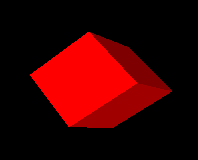
\includegraphics[width=0.9543in,height=0.772in]{ub-img/ub-img12.png}
\\\hline
Cylinder &
\texttt{DrawCylinder()} &
x, y, and z coordinates of the center, the height, the radius of the
top, the radius of the bottom. If one radius is smaller than the other,
a cone is formed.  &
\centering\arraybslash 
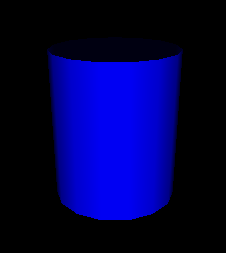
\includegraphics[width=0.7984in,height=0.689in]{ub-img/ub-img13.png} 
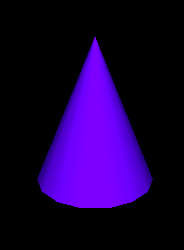
\includegraphics[width=0.7953in,height=0.689in]{ub-img/ub-img14.png}
\\\hline
Disk &
\texttt{DrawDisk()} &
x, y, and z coordinates of center, the radius of the inner circle,
and the radius of the outer circle. An additional two
angle values specify a partial disk.  &
{\centering 

\includegraphics[width=0.7866in,height=0.689in]{ub-img/ub-img15.png}
\par}

\centering\arraybslash 

\includegraphics[width=0.7866in,height=0.689in]{ub-img/ub-img16.png}
\\\hline
Solid Polygon &
\texttt{FillPolygon()} &
x, y, and z coordinates of each vertex of the polygon.  &
\centering\arraybslash 

\includegraphics[width=0.9429in,height=0.6217in]{ub-img/ub-img17.png}
\\\hline
Line &
\texttt{DrawLine()} &
x, y, and z coordinates of each vertex.  &
\centering\arraybslash 
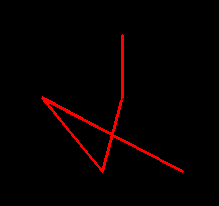
\includegraphics[width=0.9417in,height=0.5957in]{ub-img/ub-img18.png}
\\\hline
Polygon &
\texttt{DrawPolygon()} &
x, y, and z coordinates of each vertex.  &
\centering\arraybslash 
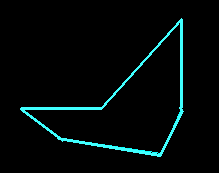
\includegraphics[width=0.9417in,height=0.6043in]{ub-img/ub-img19.png}
\\\hline
Point &
\texttt{DrawPoint()} &
x, y, and z coordinates of each point. &
\centering\arraybslash 
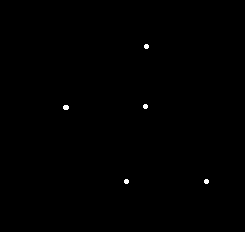
\includegraphics[width=0.9429in,height=0.5957in]{ub-img/ub-img20.png}
\\\hline
Segment &
\texttt{DrawSegment()} &
x, y, and z coordinates of each vertex. &
\centering\arraybslash 

\includegraphics[width=0.9362in,height=0.6425in]{ub-img/ub-img21.png}
\\\hline
Sphere &
\texttt{DrawSphere()} &
x, y, and z coordinates of center and the radius of the sphere.  &
\centering\arraybslash 
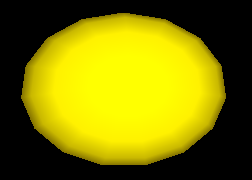
\includegraphics[width=0.9307in,height=0.6543in]{ub-img/ub-img22.png}
\\\hline
Torus &
\texttt{DrawTorus()} &
x, y, and z coordinates of the center, an inner radius and an outer
radius.  &
\centering\arraybslash 
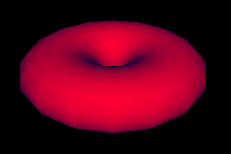
\includegraphics[width=0.9398in,height=0.6272in]{ub-img/ub-img23.png}
\\\hline
\end{supertabular}
\end{center}
\subsubsection[Coordinate Transformations]{Coordinate Transformations}
Matrix multiplications are used to calculate transformations such as
rotations on objects and the field of view.
Functions to perform several matrix operations in support of coordinate
transformation are available. The main transformation functions are
\texttt{Translate(dx,dy,dz)}, \texttt{Scale(mx,my,mz)}, and
\texttt{Rotate(a,x,y,z)}.

In many 3D graphics applications, transformations are composed as the
pieces of an object are drawn relative to one another. Transformations
are saved and restored as objects are traversed.  Unicon uses the system's
matrix stacks to keep track of the current matrix with a stack of matrices,
where the top of the stack is the current matrix.
Several functions manipulate the matrix stack. The function
\texttt{PushMatrix()} pushes a copy of the current matrix onto the
stack. By doing this the user can compose several different
transformations. The function \texttt{IdentityMatrix()} changes the
current matrix to the identity matrix. To discard the top matrix and to
return to the previous matrix, the function
\texttt{PopMatrix()} pops the top matrix off the matrix stack.

There are different matrix stacks for the projection and model view. The
projection stack contains matrices that perform calculations on
the field of view, based on the current eye
attributes. If these eye attributes are changed, previous
manipulations of the projection matrix stack are no longer valid. The
maximum depth of the projection matrix stack is two. Trying to push
more than two matrices onto the projection matrix stack will generate a
runtime error. The model view stack contains matrices to perform
calculations on objects within the scene. Transformations on the
model view stack affect the subsequently drawn objects. The
maximum depth of this stack is 32; pushing more than 32 matrixes on
the model view stack results in an error. Furthermore, only one
matrix stack can be manipulated at any given time. The function
\texttt{MatrixMode()} switches between the two matrix stacks. 

\subsubsection{Lighting and Materials}

Lighting is important in making a graphics scene appear to be 3D.
Adding lighting to a scene can be complicated. A light source can
emit different types of light. {\em Ambient\/} light has
been scattered so much that is difficult to determine the source;
backlighting in a room is an example. {\em Diffuse\/} light
comes from one direction and is central in defining what color
the object appears to be. Finally, {\em specular\/} light not only comes from
one direction, but also tends to bounce off the objects in the scene.

Applications control lighting using context attributes. For a 3D scene
in Unicon, eight lights are available. Attributes \texttt{light0}
- \texttt{light7} control the eight lights. Each light is
\texttt{on} or \texttt{off} and has the properties \texttt{diffuse},
\texttt{ambient}, \texttt{specular}, and \texttt{position}. 

Interacting with the lights, the objects in a scene may have
several material properties. The material properties are ambient,
diffuse, and specular, which are similar to the light properties, plus
emission, and shininess. If an object has an emission property, it
emits light of a specific color. Using combinations of these material
properties one can give an object the illusion of being made of plastic
or metal.

In 2D, the foreground color is controlled using the attribute \texttt{fg}.
In 3D, the \texttt{fg} attribute is extended to allow a
semi-colon separated list of material properties with the color that
property should have. The values for each of the lights follow the same
pattern. A programmer can specify colors as in the 2D graphics
facilities, or by providing comma-separated red, green, and blue
intensities as real numbers between \texttt{0.0} and \texttt{1.0}.
Examples of lighting and material properties can be found below.

Using lights and materials in Unicon was simplified by extending the
design of the 2D graphics facilities. The \texttt{fg} attribute greatly
reduces the number of lines of code needed for a scene. Thanks to this
design along with the extensive use of defaults, a programmer can use
lighting in a 3D graphics application without much effort.

\subsubsection[Textures]{Text\textstyleHeadingivChar{u}res}
Another important area of 3D graphics is textures.
Adding textures to a scene can give a scene a realistic feel.
There are several aspects to using textures. A texture
is a rectangular image that is
{\textquotedbl}glued{\textquotedbl} onto objects in a scene. The
appearance of the textured objects in the scene depends on several
pieces of information supplied by the programmer. These include the
texture image and what parts of the texture image is mapped to what
parts of the object.

The attribute \texttt{texmode} enables or disables textures,
which are disabled by default.
WAttrib({\textquotedbl}texmode=on{\textquotedbl}) enables textures.
When textures are enabled and a texture image is given, the texture
is applied to the objects drawn in the scene.

Unicon provides several formats to specify a texture image. A texture
can be a Unicon window, an image file, or a string. String textures
are encoded in one of the language standard
formats {\textquotedbl}width,pallet,data{\textquotedbl} or
{\textquotedbl}width,\#data{\textquotedbl} described in the 2D graphics
facilities. In the first case the pallet will determine what colors
appear in the texture image. In the second case, the foreground color
and background color are used. The ability to use another Unicon
window as a texture provides great flexibility for texture images,
allowing programs to create texture images dynamically.

Textures must have a height of 2\textsuperscript{n} pixels and width
of 2\textsuperscript{m} pixels where n and m are integers. If not, the
texture dimensions are automatically scaled down to the closest power
of 2. Rescaling affects application performance and may cause visual
artifacts, so it may be wise to create textures with appropriate sizes
in the first place. Examples of how to use textures specified in the
different forms are given below.

A programmer specifies a texture either by calling
\texttt{WAttrib({\textquotedbl}texture=...{\textquotedbl})}\texttt{ }or
using \texttt{Texture(t)}. These methods differ only in that a
window cannot be used as a texture with \texttt{WAttrib(),} so
\texttt{Texture()} must be called when a window is used as a texture.

A program can specify how a texture is applied to a particular object
by specifying texture coordinates and vertices. Texture
coordinates are x and y coordinates within the texture; texture
coordinate (0.0, 0.0) corresponds to the lower left corner of the
texture image. Texture coordinates are mapped to the vertices of an
object in the scene. Together, the texture coordinates and the vertices
determine what the object looks like after textures have been applied.
Since texture coordinates are complex, defaults are provided. Assigning
attribute \texttt{texcoord} the value \texttt{auto} causes system
default texture coordinates to be used. The defaults are dependent on
the type of primitive.

Non-default texture coordinates are given in several ways, such as \linebreak
\texttt{WAttrib({\textquotedbl}texcoord=}\texttt{\textit{s{\textquotedbl}}}\texttt{)}
where \texttt{\textit{s}} is a comma separated string of real number
values between \texttt{0.0} and \texttt{1.0}. Each pair of values is
taken as one texture coordinate; there must be an even number of real
values or the assignment of texture coordinates fails. One
can assign texture coordinates by calling \texttt{Texcoord(x1,y1,...)}
where \texttt{x} and \texttt{y} are real number values between
\texttt{0.0} and \texttt{1.0}. Finally one can use \texttt{Texcoord(L)}
where \texttt{L} is a list of real number texture coordinates. The
texture coordinates given by the programmer are used differently
depending on the type of primitive to be drawn. If the primitive is a
point, line, line segment, polygon, or filled polygon, then a texture
coordinate given is assigned to each vertex. If there are more texture
coordinates than vertices, unused texture coordinates are ignored. If
there are more vertices than texture coordinates the application of a
texture will fail. In order to use non-default texture coordinates
with cubes, tori, spheres, disks, and cylinders a programmer should
approximate the desired mapping with filled polygons. These
specifications are given in Table 7-6.

% \clearpage

{\centering\sffamily\bfseries
Table 7-6
\par}

{\centering\sffamily\bfseries
Texture coordinates and primitives
\par}

\begin{center}
\tablehead{}
\begin{supertabular}{|m{0.7122598in}|m{3.22956in}|m{0.9816598in}|m{0.7559598in}|}
\hline
Primitive &
Default Texture Coordinates

(from [OpenGL00] chapter 6) &
Effect of Texture Coordinates &
Picture\\\hline
Cube &
The texture image is applied to each face of the cube.  &
None &
\begin{center}
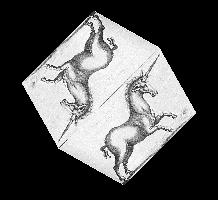
\includegraphics[width=0.6602in,height=0.6602in]{ub-img/ub-img24.jpg}
\end{center}
\\\hline
Sphere

~

~

Cylinder &
The y texture coordinate ranges linearly from 0.0 to 1.0. On spheres
this is from\newline
z= -radius to z=radius; on cylinders, from\newline
z = 0 to z = height. The x texture coordinate ranges from 0.0 at the
positive y-axis to 0.25 at the positive x-axis, to 0.5 at the
negative\newline
y-axis to 0.75 at the negative x-axis back to 1.0 at the positive
y-axis.  &
None &


\begin{center}
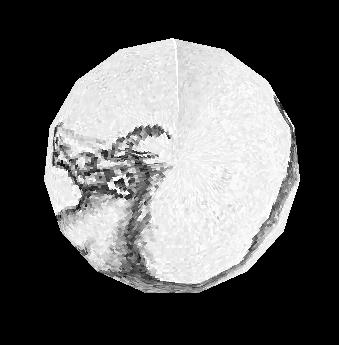
\includegraphics[width=0.6602in,height=0.6602in]{ub-img/ub-img25.jpg}
\end{center}
\begin{center}
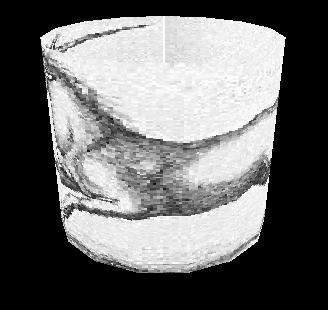
\includegraphics[width=0.6602in,height=0.6602in]{ub-img/ub-img26.jpg}
\end{center}
\\\hline
Filled Polygon

~

Line

~

~

Polygon

~

Segment

~
 &
The x and y texture coordinates are given by
p\textsubscript{1}x\textsubscript{0}+p\textsubscript{2}y\textsubscript{0}+p\textsubscript{3}z\textsubscript{0}+p\textsubscript{4}w\textsubscript{0}
 &
A texture coordinate is assigned to a vertex.  &


\begin{center}
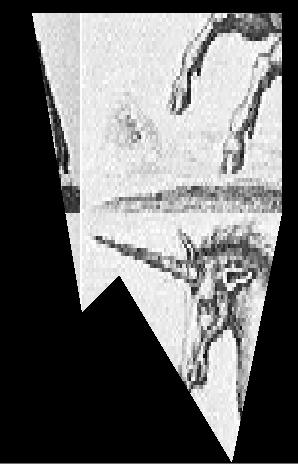
\includegraphics[width=0.6602in,height=0.6602in]{ub-img/ub-img27.jpg}
\end{center}
\begin{center}

\includegraphics[width=0.6602in,height=0.6602in]{ub-img/ub-img28.jpg}
\end{center}
\begin{center}

\includegraphics[width=0.6602in,height=0.6602in]{ub-img/ub-img29.jpg}
\end{center}
\begin{center}

\includegraphics[width=0.6602in,height=0.6602in]{ub-img/ub-img30.jpg}
\end{center}
\\\hline
Torus &
The x and y texture coordinates are given by
p\textsubscript{1}x\textsubscript{0}+p\textsubscript{2}y\textsubscript{0}+p\textsubscript{3}z\textsubscript{0}+p\textsubscript{4}w\textsubscript{0}
&
None &
\begin{center}
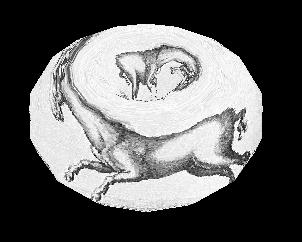
\includegraphics[width=0.6693in,height=0.698in]{ub-img/ub-img31.jpg}
\end{center}
\\\hline
\end{supertabular}
\end{center}

\subsubsection{Examples}

\paragraph{Changing Context Attributes}
The user can change attributes throughout a program. Multiple
attributes can be changed with one call to \texttt{WAttrib()}.
The following line of code changes the eye
position to (0.0, 0.0, 5.0) and the eye direction to look at the
positive z-axis. An assignment to \texttt{eyepos}, \texttt{eyedir},
\texttt{eyeup} or \texttt{eye}
redraws the screen; a given call to \texttt{WAttrib()} will only redraw the
scene once.

\iconcode{
\>   WAttrib({\textquotedbl}eyepos=0.0,0.0,5.0{\textquotedbl},{\textquotedbl}eyedir=0.0,0.0,1.0{\textquotedbl})}

The values of the attributes can also be read by using the function
\texttt{WAttrib()}. The current eye position could be stored in variable
\texttt{ep} by the call:

\iconcode{
\>   ep := WAttrib({\textquotedbl}eyepos{\textquotedbl})}

\paragraph{Drawing Primitives}
Here is an example that uses some of the drawing primitives. 

\iconcode{
\>   Fg(w, {\textquotedbl}ambient yellow{\textquotedbl}) \\
\>   DrawDisk(w, 0.4, -0.5, -4.0, 0.0, 1.0, 0.0, 0.0, 1.0,
		 0.5, -5.0, 0.5, 1.0) \\
\>   Fg(w, {\textquotedbl}diffuse white{\textquotedbl}) \\
\>   DrawDisk(w, 0.4, -0.5, -4.0, 0.0, 1.0, 0.0, 
		225.0,1.0, 0.5, -5.0, 0.5,1.0,0.0,125.0) \\
\>   Fg(w, {\textquotedbl}ambient pink{\textquotedbl}) \\
\>   DrawCylinder(w, 0.0, 1.0, -5.0, 1.0, 0.5, 0.3) \\
\>   Fg(w, {\textquotedbl}specular navy{\textquotedbl}) \\
\>   DrawDisk(w, -0.5, -0.5, -2.0, 0.5, 0.3) \\
\>   Fg(w, {\textquotedbl}emission green{\textquotedbl}) \\
\>   DrawSphere(w, 0.5, 1.0, -3.0, 0.5) \\
\>   WAttrib(w, {\textquotedbl}light0=on, diffuse white{\textquotedbl})
}

% \clearpage

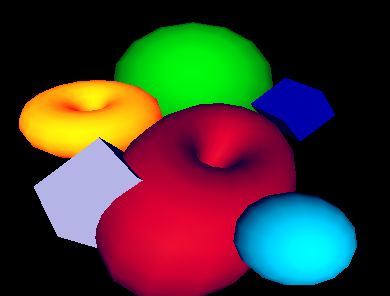
\includegraphics[width=2.8071in,height=2.1335in]{ub-img/ub-img32.png} 

{\sffamily\bfseries Figure 7-2:}
{\sffamily 3D Drawing Primitives Made From Various Materials}

\bigskip

The function \texttt{Fg()} specifies the material properties of
subsequently drawn objects that affect their color and appearance.
In this example, a cube with a diffuse green material is
drawn with sides of length 0.7. Then a sphere with a diffuse purple and
ambient blue material is drawn with radius 0.5 and center (0.4, -0.5,
-4.0). Next a diffuse yellow and ambient grey torus with center (-1.0,
0.4, -4.0), an inner radius of 0.4, and an outer radius of 0.5 is
drawn. Finally a filled polygon with a diffuse red material property
and three vertices, (0.25, -0.25, -1.0), (1.0, 0.25, -4.0) and
(1.3, -0.4, -3.0) is drawn. 

\paragraph{Lighting and Materials}
Up to eight lights can be used in each scene. The
lights are control by the context attributes \texttt{light0} through
\texttt{light7}.
Each light has five properties that can be changed throughout the
program, ambient, diffuse, specular, position, and on/off. The
properties of a light can be set using \texttt{WAttrib()} to set one of
\texttt{light0} through \texttt{light7}. To turn on or off a light,
assign on or off to the light, followed by a comma and a lighting value.
A lighting value is a string which contains one or more semi-colon
separated lighting properties. A lighting property is of the form
\newline
 \ \ [diffuse{\textbar}ambient{\textbar}specular] \textit{color
name}\newline
If one does not want to turn on or off a light, a lighting value is
specified. The following call turns light1 on and gives it diffuse
yellow and ambient gold lighting properties. 

\ \ \ WAttrib(w, {\textquotedbl}light1=on, diffuse yellow; ambient
gold{\textquotedbl})

The following expression sets \texttt{light0} to the default values for
the lighting properties.

\iconcode{
\>   WAttrib(w, {\textquotedbl}light0=diffuse white; ambient black; \_ \\
\>   \ \ \ \ \ \ \ \ \ \ \ \ \ \ \ \ \ \ \ specular white; position
0.0, 1.0, 0.0{\textquotedbl})}

The next example shows the difference between the different types of
lighting that can be used in a scene. Each window is the same scene
rendered using different lighting. The upper right scene has an ambient
blue-green light. The upper left scene was drawn using a diffuse
blue-green light. The lower right scene uses only a specular blue-green
light. The scene in the lower left uses all three types of lighting.

{\centering 
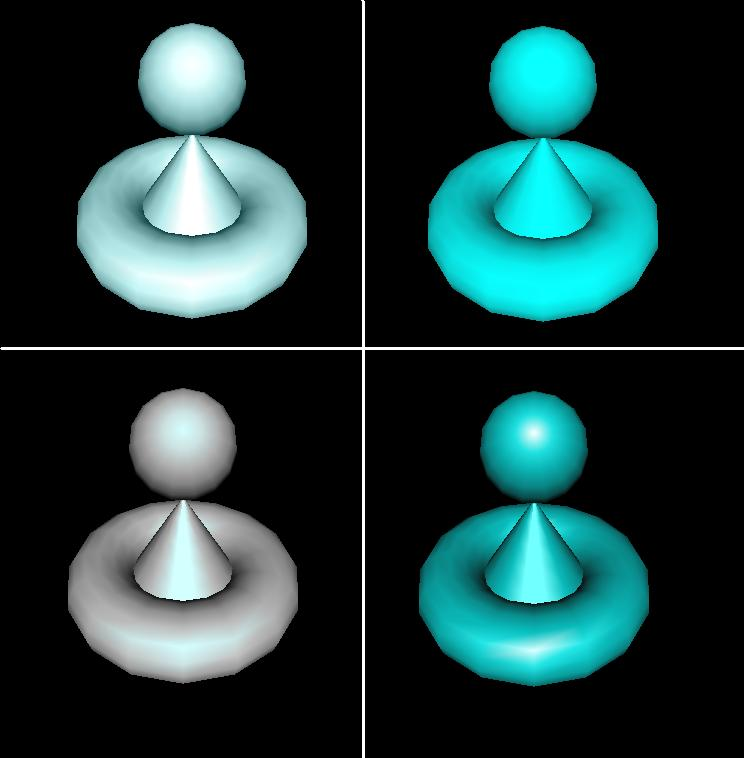
\includegraphics[width=2.1957in,height=2.2346in]{ub-img/ub-img33.jpg}
\par}

{\sffamily\bfseries Figure 7-3:}
{\sffamily Different Types of Lighting}

\bigskip

\iconcode{
\>   w :=
open({\textquotedbl}ambient.icn{\textquotedbl},{\textquotedbl}gl{\textquotedbl},
{\textquotedbl}bg=black{\textquotedbl},
{\textquotedbl}size=400,400{\textquotedbl}) \\
\>   WAttrib(w,{\textquotedbl}light0=on, ambient
blue-green{\textquotedbl},{\textquotedbl}fg=specular
white{\textquotedbl}) \\
\>   DrawCylinder(w, 0.0, -0.2, -3.5, 0.75, 0.5, 0.0) \\
\>   DrawTorus(w,0.0, -0.2, -3.5, 0.3, 0.7) \\
\>   DrawSphere(w,0.0, 0.59, -2.2, 0.3) \\
\ \\
\>   x :=
open({\textquotedbl}diffuse.icn{\textquotedbl},{\textquotedbl}gl{\textquotedbl},
{\textquotedbl}bg=black{\textquotedbl},
{\textquotedbl}size=400,400{\textquotedbl}) \\
\>   WAttrib(x,{\textquotedbl}light0=on, diffuse
blue-green{\textquotedbl},{\textquotedbl}fg=specular
white{\textquotedbl}) \\
\>   DrawCylinder(x, 0.0, -0.2, -3.5, 0.75, 0.5, 0.0) \\
\>   DrawTorus(x,0.0, -0.2, -3.5, 0.3, 0.7) \\
\>   DrawSphere(x, 0.0, 0.59, -2.2, 0.3) \\
\ \\
\>   y :=
open({\textquotedbl}specular.icn{\textquotedbl},{\textquotedbl}gl{\textquotedbl},
{\textquotedbl}bg=black{\textquotedbl},
{\textquotedbl}size=400,400{\textquotedbl}) \\
\>   WAttrib(y,{\textquotedbl}light0=on,specular
blue-green{\textquotedbl},{\textquotedbl}fg=specular
white{\textquotedbl}) \\
\>   DrawCylinder(y, 0.0, -0.2, -3.5, 0.75, 0.5, 0.0) \\
\>   DrawTorus(y, 0.0, -0.2, -3.5, 0.3, 0.7) \\
\>   DrawSphere(y, 0.0, 0.59, -2.2, 0.3) \\
\ \\
\>   z :=
open({\textquotedbl}all.icn{\textquotedbl},{\textquotedbl}gl{\textquotedbl},
{\textquotedbl}bg=black{\textquotedbl},
{\textquotedbl}size=400,400{\textquotedbl}) \\
\>   WAttrib(z, {\textquotedbl}light0=on, diffuse blue-green; \_ \\
\>   \ specular blue-green; ambient
blue-green{\textquotedbl},{\textquotedbl}fg=specular
white{\textquotedbl}) \\
\>   DrawCylinder(z, 0.0, -0.2, -3.5, 0.75, 0.5, 0.0) \\
\>   DrawTorus(z, 0.0, -0.2, -3.5, 0.3, 0.7) \\
\>   DrawSphere(z, 0.0, 0.59, -2.2, 0.3)
}

Materials can be changed using \texttt{Fg()} or \texttt{WAttrib()}
with the context attribute \texttt{fg}. A material value is a string
containing one or more
semi-colon separated material properties. Material properties are of
the form\newline
\ \ [ diffuse {\textbar} ambient {\textbar} specular {\textbar} emission
] \textit{color name} \newline
or \newline
\ \ {\textquotedbl}shininess n{\textquotedbl}, where n is some integer
in the range 0 {\textless}= n
{\textless}= 128.

The default material property type is diffuse, so the call
Fg({\textquotedbl}red{\textquotedbl}) is equivalent to
Fg({\textquotedbl}diffuse red{\textquotedbl}). For shininess, a value
of 0 spreads specular light broadly across an object and a value of 128
focuses specular light at a single point. The following line of code
changes the current material property to diffuse green and ambient
orange. 

\iconcode{
\ \ \ WAttrib(w, {\textquotedbl}fg=diffuse green; ambient
orange{\textquotedbl})
}

\noindent The default values of the material properties are given in the
following example. 

\iconcode{
   Fg(w, \textrm{{\textquotedbl}}diffuse light grey; ambient grey;
specular black; emission black; \_ \\
\>\> shininess 50\textrm{{\textquotedbl}})}

\noindent Figure 7-4 shows the effects of emission color on an object. 

\bigskip

{\centering 
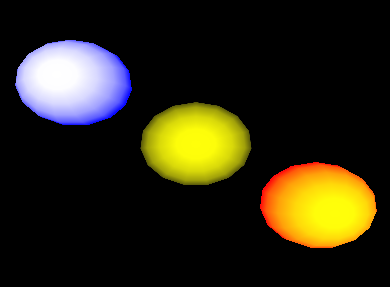
\includegraphics[width=2.5583in,height=1.8835in]{ub-img/ub-img34.png}
\par}

{\sffamily\bfseries Figure 7-4:}
{\sffamily Mixing Emission and Diffuse Material Properties}

\bigskip

\iconcode{
\>   Fg(w, {\textquotedbl}emission blue; diffuse yellow{\textquotedbl}) \\
\>   DrawSphere(w, -1.5, 1.0, -5.0, 0.7) \\
\>   Fg(w, {\textquotedbl}emission black{\textquotedbl}) \\
\>   DrawSphere(w, 0.0, 0.0, -5.0, 0.7) \\
\>   Fg(w, {\textquotedbl}emission red{\textquotedbl}) \\
\>   DrawSphere(w, 1.5, -1.0, -5.0, 0.7)
}

In the above example, three yellow spheres are drawn. An emission
color of blue makes the sphere appear white with a
blue ring. With a red emission color, the sphere remains yellow, but
now has an orange-red ring. The middle sphere shows the effect of
having no emission color. In order to obtain the diffuse yellow sphere
in the center, the emission color was changed to black, without
changing the diffuse property.

\paragraph{Textures}
This section contains several examples of the use of textures in a
scene. There are several ways to specify the texture image: a file, an
image string, or another window. The following example
uses a file as a texture. A .gif image of a map of the world is used
to texture a torus using the default texture coordinates.

\clearpage

{\centering 
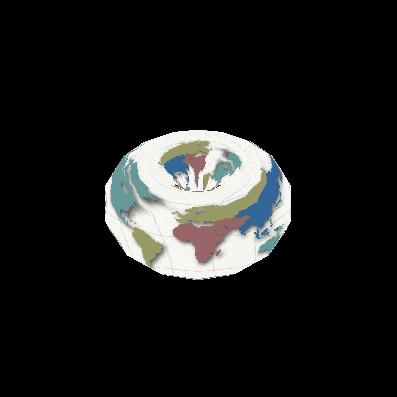
\includegraphics[width=2.0583in,height=2.0583in]{ub-img/ub-img35.jpg}
\par}

{\sffamily\bfseries Figure 7-5:}
{\sffamily A Texture from a GIF Image is Mapped onto a Torus}

\bigskip

\iconcode{
\>   WAttrib(w, {\textquotedbl}texmode=on{\textquotedbl},
{\textquotedbl}texture=map.gif{\textquotedbl}) \\
\>   DrawTorus(w, 0.0, 0.0, -3.0, 0.3, 0.4)
}

Instead of using \texttt{WAttrib(w,
{\textquotedbl}texture=map.gif{\textquotedbl})}\texttt{ }to specify the
.gif file, a call to \texttt{Texture(w,
{\textquotedbl}map.gif{\textquotedbl})} could be used to obtain the
same result.

The next example uses an image string to specify a
texture image. The string used for this example is taken from Graphics
Programming in Icon [Griswold98] page 156. This string is used as a
texture on a cube using the default texture coordinates. 

\bigskip

{\centering 
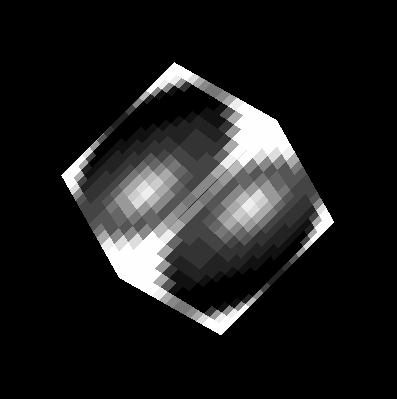
\includegraphics[width=2.0508in,height=2.0571in]{ub-img/ub-img36.jpg}
\par}

{\sffamily\bfseries Figure 7-6:}
{\sffamily A Texture Supplied via an Image String}

\bigskip

\iconcode{
\ \ \ WAttrib(w, {\textquotedbl}texmode=on{\textquotedbl}) \\
\>   sphere:= {\textquotedbl}16,g16, FFFFB98788AEFFFF{\textquotedbl}
{\textbar}{\textbar} \\
\>   \ \ {\textquotedbl}FFD865554446AFFF FD856886544339FF
E8579BA9643323AF{\textquotedbl}{\textbar}{\textbar} \\
\>   \ \ {\textquotedbl}A569DECA7433215E 7569CDB86433211A
5579AA9643222108{\textquotedbl}{\textbar}{\textbar} \\
\>   \ \ {\textquotedbl}4456776533221007 4444443332210007
4333333222100008{\textquotedbl}{\textbar}{\textbar} \\
\>   \ \ {\textquotedbl}533322221100000A 822222111000003D
D41111100000019F{\textquotedbl}{\textbar}{\textbar} \\
\>   \ \ {\textquotedbl}FA200000000018EF FFA4000000028EFF
FFFD9532248BFFFF{\textquotedbl} \\
\>   Texture(w, sphere) \\
\>   DrawCube(w, 0.0, 0.0, -3.0, 1.2)
}

The next example shows the use of a Unicon window as a texture. An
image of a lamp is drawn on the first window in
{\textquotedbl}\texttt{gl{\textquotedbl}} mode. This window is then
used as a texture on a cylinder. The same method can be
used to embed 2D window contents in 3D scenes. Note that in the
following code the first window is opened with size 256 x 256. Texture
images must have height and width that are powers of 2, or the system
must rescale them. The default coordinates for cylinders are used.

{\centering\color{green}
 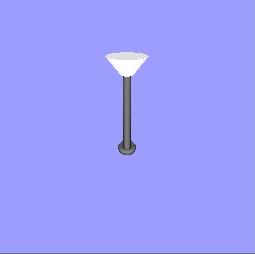
\includegraphics[width=1.4492in,height=1.4335in]{ub-img/ub-img37.jpg}
\texttt{ \ \ }

\includegraphics[width=1.939in,height=1.952in]{ub-img/ub-img38.jpg}
\texttt{ \ \ }
\par}

{\sffamily\bfseries Figure 7-7:}
{\sffamily A Texture Obtained from Another Window{\textquotesingle}s Contents}

\bigskip

\iconcode{
\>   w :=
open({\textquotedbl}win1{\textquotedbl},{\textquotedbl}gl{\textquotedbl},{\textquotedbl}bg=light
blue{\textquotedbl},{\textquotedbl}size=256,256{\textquotedbl}) \\
\>   Fg(w, {\textquotedbl}emission pale grey{\textquotedbl}) \\
\>   PushMatrix(w) \\
\>   Rotate(w, -5.0, 1.0, 0.0, 0.0) \\
\>   DrawCylinder(w, 0.0, 0.575, -2.0, 0.15, 0.05, 0.17) \\
\>   PopMatrix(w) \  \\
\>   Fg(w, {\textquotedbl}diffuse grey; emission black{\textquotedbl}) \\
\>   PushMatrix(w) \\
\>   Rotate(w, -5.0, 1.0, 0.0, 0.0) \\
\>   DrawCylinder(w, 0.0, 0.0, -2.5, 0.7, 0.035, 0.035) \\
\>   PopMatrix(w) \ \ \ \ \ \ \ \ \ \ \ \ \ \  \\
\>   DrawTorus(w, 0.0, -0.22, -2.5, 0.03, 0.06) \\
\>   DrawTorus(w, 0.0, 0.6, -2.5, 0.05, 0.03) \\
\ \\
\>   w2 :=
open({\textquotedbl}win2.icn{\textquotedbl},{\textquotedbl}gl{\textquotedbl},{\textquotedbl}bg=black{\textquotedbl},{\textquotedbl}size=400,400{\textquotedbl}) \\
\>   WAttrib(w2, {\textquotedbl}texmode=on{\textquotedbl}) \\
\>   Texture(w2, w)  \\
\>   Fg(w2, {\textquotedbl}diffuse purple; ambient blue{\textquotedbl}) \\
\  \\
\>   DrawCylinder(w2, 0.0, 0.0, -3.5, 1.2, 0.7, \ 0.7)
}

The next two examples illustrate the use of the default texture
coordinates versus texture coordinates specified by the programmer. In
both examples, a bi-level image is used as the texture image. The
format for such a string is described in section 2.7. This image is
taken from Graphics Programming in Icon page 159. The first example
uses the default texture coordinates for a filled polygon, which in
this case is just a square with sides of length one. In this case the
default texture coordinates are as follows. The coordinate (0.0,
0.0)\texttt{ }of the texture image is mapped to the vertex\texttt{
}(0.0, 0.0, -2.0) of the square, (0.0, 1.0)\texttt{ }is mapped to (0.0,
1.0, -2.0)\texttt{, }(1.0, 1.0)\texttt{ }is mapped to (1.0, 1.0, -2.0),
and (1.0, 0.0)\texttt{ }is mapped to (1.0, 0.0, -2.0).

{\centering 
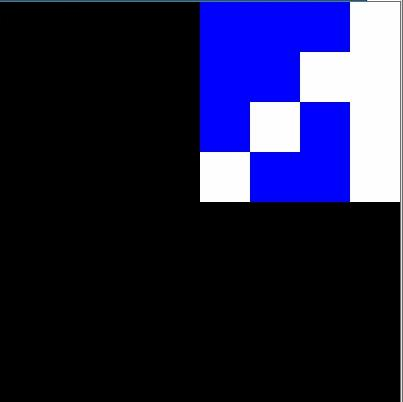
\includegraphics[width=1.8335in,height=1.8335in]{ub-img/ub-img39.jpg}
\par}

{\sffamily\bfseries Figure 7-8:}
{\sffamily Default Texture Coordinates}

\bigskip

\iconcode{
\>   WAttrib(w,{\textquotedbl}fg=white{\textquotedbl},{\textquotedbl}bg=blue{\textquotedbl},{\textquotedbl}texmode=on{\textquotedbl},{\textquotedbl}texture=4,\#8CA9{\textquotedbl}) \\
\>   Fg(w, {\textquotedbl}diffuse purple; ambient blue{\textquotedbl}) \\
\>   FillPolygon(w, 0.0, 0.0, -2.0, 0.0, 1.0, -2.0, \\
\>   \ \ \ \ \ \ \ \ \ \ \ \ \ \ \ 1.0, 1.0, -2.0, 1.0, 0.0, -2.0)
}

This example uses the same texture image and the same object to be
textured, but instead uses the texture coordinates (0.0, 1.0), (1.0,
1.0), (1.0, 1.0), and (1.0, 0.0). So the coordinate (0.0, 1.0) of the
texture image is mapped to the vertex (0.0, 0.0, -2.0) of the square,
(1.0, 1.0) is mapped to (0.0, 1.0, -2.0),(1.0, 1.0) is mapped to (1.0,
1.0, -2.0), and (1.0, 0.0) is mapped to (1.0, 0.0, -2.0).

\bigskip

{\centering 

\includegraphics[width=2.0307in,height=2.0311in]{ub-img/ub-img40.jpg}
\par}

{\sffamily\bfseries Figure 7-9:}
{\sffamily Custom Texture Coordinates}

\bigskip

\iconcode{
\>   Wattrib(w,{\textquotedbl}fg=white{\textquotedbl},{\textquotedbl}bg=blue{\textquotedbl},{\textquotedbl}texmode=on{\textquotedbl},{\textquotedblright}texture=4,\#8CA9{\textquotedblright}, \\
\>   \ \ \ \ \ \ \ \ \ \ {\textquotedbl}texcoord=0.0, 1.0, 1.0, 1.0,
1.0, 1.0, 1.0, 0.0{\textquotedbl}) \\
\>   FillPolygon(w, 0.0, 0.0, -2.0, 0.0, 1.0, -2.0, \\
\>   \ \ \ \ \ \ \ \ \ \ \ \ \ \ \ 1.0, 1.0, -2.0, 1.0, 0.0, -2.0)
}

Instead of using \texttt{WAttrib()} with the attribute \texttt{texcoord},
the function \texttt{Texcoord()} could be used. So the line 

\iconcode{
\>   WAttrib(w,{\textquotedbl}texcoord=0.0, 1.0, 1.0, 1.0, 1.0,
1.0,1.0, 0.0{\textquotedbl})}

\noindent
could be replaced by 

\iconcode{
\>   Texcoord(w, 0.0, 1.0, 1.0, 1.0, 1.0, 1.0,1.0, 0.0)}

\paragraph[A Larger Textures Example]{A Larger Textures Example}
The following more complicated example uses many features of
the Unicon 3D graphics facilities described in the previous sections.
This example also illustrates the effect of adding texture to a scene.
The scene on the left is a scene drawn without any texturing.
The scene on the right contains texturing. The scene on the right is a
much more realistic scene than the one on the left. 

All textures used in the textured scene, except for the unicorn, where
captured using a digital camera. These images were then converted into
.gif files and scaled to width and height of 2\textsuperscript{n}.
Directly using an image file is one feature of the Unicon 3D graphics
facilities that makes adding textures simpler than using OpenGL. 

\bigskip

{\color{green}
 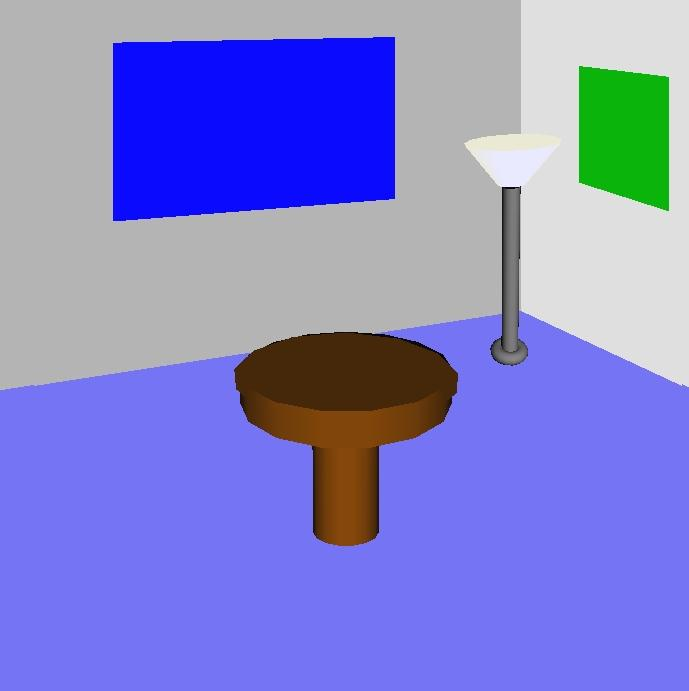
\includegraphics[width=2.6543in,height=2.6693in]{ub-img/ub-img41.jpg}
\textbf{ \ \ \ \ \ \ \ \ \ \ \ \ \ }
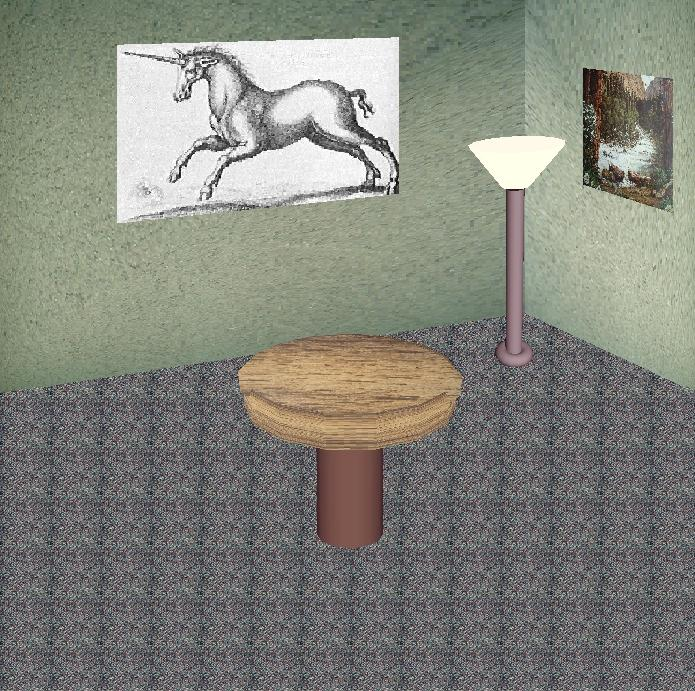
\includegraphics[width=2.6846in,height=2.6693in]{ub-img/ub-img42.jpg} }

{\sffamily\bfseries Figure 7-10:}
{\sffamily\bfseries Untextured and Textured Versions of the Same Scene}

\bigskip

\iconcode{
procedure main() \\
\>   \&window
:=open({\textquotedbl}textured.icn{\textquotedbl},{\textquotedbl}gl{\textquotedbl},{\textquotedbl}bg=black{\textquotedbl},{\textquotedbl}size=700,700{\textquotedbl}) \\
\ \\
\>   \# Draw the floor of the room \\
\>   WAttrib({\textquotedbl}texmode=on{\textquotedbl},
{\textquotedbl}texture=carpet.gif{\textquotedbl}) \\
\>   FillPolygon(-7.0, -0.9, -14.0, -7.0, -7.0, -14.0, \\
\>\>\> 7.0, -7.0,
-14.0, 7.0, -0.9, -14.0, 3.5, 0.8, -14.0) \\
\ \\
\>   \# Draw the right wall \\
\>   Wattrib({\textquotedbl}texture=wall1.gif{\textquotedbl},
{\textquotedbl}texcoord=0.0, 1.0, 0.0, 0.0, 1.0, 0.0, 1.0,
1.0{\textquotedbl}) \\
\>   FillPolygon(2.0, 4.0, -8.0, 8.3, 8.0, -16.0, 8.3, -1.2, -16.0,
2.0, 0.4, -8.0) \\
\ \\
\>   \# Draw the left wall \\
\>   WAttrib({\textquotedbl}texture=wall2.gif{\textquotedbl}) \\
\>   FillPolygon(2.0, 4.0 ,-8.0, -9.0, 8.0, -16.0, -9.0,-1.2,-16.0,
2.0, 0.4, -8.0) \\
\ \\
\>   \# Draw a picture \\
\>   Wattrib({\textquotedbl}texture=poster.gif{\textquotedbl},
{\textquotedbl}texcoord=0.0, 1.0, 0.0, 0.0, 1.0, 0.0, 1.0,
1.0{\textquotedbl}) \\
\>   FillPolygon(1.0, 1.2, -3.0, 1.0, 0.7, -3.0, 1.2, 0.5, -2.6, 1.2,
1.0, -2.6) \\
\>   \# Draw another picture \\
\>   Wattrib({\textquotedbl}texture=unicorn.gif{\textquotedbl},
{\textquotedbl}texcoord=1.0, 0.0, 0.0, 0.0, 0.0, 1.0, 1.0,
1.0{\textquotedbl}) \\
\>   FillPolygon(0.8, 2.0, -9.0, -3.0, 1.6, -9.0, 3.0, 3.9,-9.0, 0.8,
4.0, -9.0)
\ \\
\>   \# Draw the lamp \\
\>   WAttrib({\textquotedbl}texmode=off{\textquotedbl}) \\
\>   PushMatrix() \\
\>   Translate(0.7, 0.20, -0.5) \\
\>   Fg({\textquotedbl}emission pale weak yellow{\textquotedbl}) \\
\>   PushMatrix() \\
\>   Rotate(-5.0, 1.0, 0.0, 0.0) \\
\>   Rotate( 5.0, 0.0, 0.0, 1.0) \\
\>   DrawCylinder(-0.05, 0.570, -2.0, 0.15, 0.05, 0.17) \\
\>   PopMatrix() \\
\>   Fg({\textquotedbl}diffuse grey; emission black{\textquotedbl}) \\
\>   PushMatrix() \\
\>   Rotate(-5.0, 1.0, 0.0, 0.0) \\
\>   Rotate( 6.0, 0.0, 0.0, 1.0) \\
\>   DrawCylinder(0.0, 0.0, -2.5, 0.7, 0.035, 0.035) \\
\>   PopMatrix() \\
\>   PushMatrix() \\
\>   Rotate(6.0, 0.0, 0.0, 1.0) \\
\>   DrawTorus(-0.02, -0.22, -2.5, 0.03, 0.05) \\
\>   PopMatrix() \  \\
\>   PopMatrix()
\ \\
\>   \# Draw the table  \\
\>   WAttrib({\textquotedbl}texcoord=auto{\textquotedbl},
{\textquotedbl}texmode=on{\textquotedbl},
{\textquotedbl}texture=table.gif{\textquotedbl}) \\
\ \\
\>   PushMatrix() \\
\>   Rotate(-10.0, 1.0, 0.0,0.0) \\
\>   DrawCylinder(0.0, 0.2, -2.0, 0.1, 0.3, 0.3) \\
\>   PopMatrix() \\
\ \\
\>   PushMatrix() \\
\>   Translate(0.0, -0.09, -1.8) \\
\>   Rotate(65.0, 1.0, 0.0, 0.0) \\
\>   DrawDisk(0.0, 0.0, 0.0, 0.0, 0.29)  \\
\>   PopMatrix() \\
\ \\
\>   WAttrib({\textquotedbl}texmode=off{\textquotedbl},
{\textquotedbl}fg=diffuse weak brown{\textquotedbl}) \\
\>   PushMatrix() \\
\>   Rotate(-20.0, 1.0, 0.0,0.0) \\
\>   DrawCylinder(0.0, 0.2, -2.2, 0.3, 0.1, 0.1) \\
\>   PopMatrix() \\
\>   while (e := Event()) \~{}== {\textquotedbl}q{\textquotedbl} do \{ \\
\>   \ \ \ write(image(e), {\textquotedbl}: {\textquotedbl}, \&x,
{\textquotedbl},{\textquotedbl}, \&y) \\
\>   \ \ \ \} \\
end
}

In order to apply textures to the scene, texturing must be turned
on. Next, the texture to be applied is specified. The floor of the
scene is drawn using a filled polygon. The default texture coordinates
are used to apply the carpet texture to the floor of the room. The
tiled appearance on the floor of the room is caused by the use of the
default texture coordinates. This can be avoided using user-supplied
texture coordinates, as is done for the textures that
are applied to the walls and the pictures in the room. 

The lamp does not have a texture, so it is necessary
to turn off texturing before drawing the lamp. Also for the lamp to be
centered properly in the room, transformations are used. Matrices are
used to isolate the transformations of the lamp. Finally to draw
the table with a textured top and an untextured base, two cylinders and
a disk are used. Texturing is applied to a cylinder and the disk.
Notice the call 

\iconcode{
\>   WAttrib(w, {\textquotedbl}texcoord=auto{\textquotedbl})
}

\noindent
This resets the texture coordinates to the defaults. Finally, texturing
is turned off to draw the base of the table.

\subsubsection{Animation}

Graphics animation is performance sensitive, and Unicon is slower than
systems programming languages such as C and C++. Nevertheless, it is
possible to write 3D animations in Unicon with acceptable frame rates.

3D animations redraw the entire scene each time an object moves or
the user changes point of view. An application can call \texttt{EraseArea()}
followed by the appropriate graphics primitives to redraw a scene, but
the results often appear to flicker. It is better to let
Unicon{\textquotesingle}s runtime system do the redrawing. Unicon
maintains a \textit{display list} of graphics operations to execute
whenever the screen must be redrawn; these operations are effectively
everything since the last \texttt{EraseArea()}. The display list for a window
can be obtained by calling \texttt{WindowContents()}. The elements of the list
are Unicon records and lists containing the string names and parameters
of graphics primitives. For example, a call to \texttt{DrawSphere(w,x,y,z,r)}
returns (and adds to the display list) a record
\texttt{gl\_sphere({\textquotedbl}DrawSphere{\textquotedbl},x,y,z,r)}. Instead
of redrawing the entire scene to move an object, you can
modify its display list record and call \texttt{Refresh()}. The following code
fragment illustrates animation by causing a ball to slide up and down.
In order to \textit{bounce}, the program would need to incorporate
physics. 

\iconcode{
sphere := DrawSphere(w, x, y, z, r) \\
increment := 0.2 \\
every i := 1 to 100 do \\
\>   every j := 1 to 100 do \{ \\
\>   \ \ \ sphere.y +:= increment \\
\>   \ \ \ Refresh(w) \\
\>   \ \ \ \}
}

This technique gives animation rates of 100-200 frames per second on
current midrange PC hardware. Unicon supports smooth animation for a
number of objects which varies widely depending on the underlying
graphics hardware and software.

\subsubsection{Selective Rendering and Object Selection}

Many 3D applications model scenes with far more objects than are needed
at any particular instant. For example, a virtual building might have
many rooms on multiple floors, but only a small fraction is visible
from any particular location. The 3D facilities remove objects that are
not visible, but doing so becomes too slow for large numbers of
objects. An application with a large scene will generally have to
perform at least approximate visibility calculations to achieve smooth
animation. Such visibility calculations can be performed for each
frame, and if the visible objects change, the scene can be re-rendered
by rebuilding the display list from scratch. At this point
Unicon{\textquotesingle}s speed can be an issue, as discussed in the
previous section.

The function \texttt{WSection()} comes to the rescue. It plays two vital
roles. First, it allows portions of the display list to be skipped
during rendering, without having to rebuild the display list. Second,
it forms the basis for specifying portions of the display list that the
user may select (click on) when interacting with the scene. In both
cases, calls to \texttt{WSection()} come in pairs, first a call
\texttt{WSection(s)} identifies a portion of the display list of
interest, then the sequence of 3D calls to render some object or
portion of the scene, then a call to \texttt{WSection()} defines the
end of that section. Parameter \texttt{s} must be a unique string name
or identifier for the section.

The call to create a new section returns a record that contains a field
named \texttt{skip}. Setting \texttt{skip} to a non-null value causes the
section to be omitted whenever the scene is redrawn.
Using \texttt{WSection()} for 3D user input is similar. A program calls
\texttt{WAttrib({\textquotedblleft}pick=on{\textquotedblright})} to
turn on 3D selection, after which keyword \texttt{\&pick} generates the
identifying names for all objects intersected by the ray from the
camera through the (x,y) screen location where the mouse was located on
the last call to \texttt{Event()}.

\section*{Summary}

Graphics are ubiquitous in modern applications. Unicon provides 2D and
3D graphics capabilities that are easy to use, portable building blocks
for many programs. The 2D facilities are mature; the 3D interface is
new and will evolve. Many elements of the 2D graphics system are used
in the 3D graphics interface. Further integration of the 2D and 3D
graphics systems is likely in the future.


\ \\ \bigskip
\clearpage

\chapter{Threads}

Threads are building blocks for concurrent (also known as
\emph{parallel}) execution. In a concurrent program, the instructions
specify multiple things to compute at the same time, during some or
most of the program run.  On a classic single-processor system these
computations will only happen one at a time, but on most modern
multiprocessor and multicore systems, the hardware is designed to do
several computations at once, and if your program does not ask for as
much, it is underutilizing (sometimes severely) the platform.

This chapter describes concurrency in Unicon. It is based on Unicon
Technical Report 14; UTR14 on the unicon.org site may amend or supercede
this chapter with added features in the future.  Threads are an extension
of the co-expression type described in Chapter 4 and the system interface
described in Chapter 5.  Consulting those chapters may be helpful in
studying this one.

Concurrent programming introduces techniques, concepts, and
difficulties that do not exist in sequential programs. In some
situations concurrent programming is a natural way to write programs,
such as a server where threads serve different clients. In other
situations, concurrent programming improves performance. Long-running
programs can run faster by having several threads running
cooperatively on several CPU cores, or programs that do a lot of slow
I/O operations can allow other non-blocked threads to proceed and
utilize the CPU. However, for programs that have a lot of dependencies
and are sequential in nature, the complexities of parallelizing them
can outweigh the benefits.

This chapter is not a comprehensive concurrent programming guide. It
assumes that the reader has some basic knowledge about threads, their
programming techniques, and problems, such as synchronization and race
conditions. Readers who are unfamiliar with concurrency can refer to a
myriad of resources such as [Andr83] or [Bute97] for an
overview. Since Unicon's concurrency facilities are implemented on top
of POSIX threads (pthreads), many of the concepts from pthreads
programming apply, often with more concise, or higher-level ways of
writing things.

\section{Threads and Co-Expressions}

Co-expressions are independent, explicitly sequential execution
contexts.  Only one co-expression is active at any given moment. When
a co-expression is activated, the calling co-expression blocks until
the child co-expression returns the execution to it or fails. Threads,
on the other hand, can run simultaneously and independently. Threads
in Unicon are like special co-expressions that are marked to run
asynchronously.

In a concurrent program with two or more threads, each thread has its
own program counter, stack pointer, and other CPU registers. However,
all of the threads in a program share the address space, open files,
and many other pieces of process-wide information. This enables very
fast communication and cooperation between threads, which leads to
less blocking, faster execution and more efficient use of resources.

Unicon programs start execution in the \texttt{main()} procedure. In a
multi-thread programming environment, the procedure \texttt{main()} is
the entry point for a special thread referred to as the \emph{main
thread}. This main thread is created by the operating system when the
program begins execution.  The main thread can create new threads,
which can create even more threads.  Each thread has an entry point,
where it begins executing.  Usually this is a procedure but it can be
any Unicon expression, as is the case for co-expressions.  When a
thread first starts running in the entry point, it goes on its own
execution path, separate from the thread that created it, which
continues to run. A thread never returns.  When it ends, it simply
terminates; other threads continue to run. An important exception is
the main thread; if the main thread ends, the whole program ends. If
there are any other threads running, all of them will be terminated.

Since the emergence of the first computer, processors have been
increasing in computational power. CPU speeds grew faster than almost
all of the other units in the computer, especially the I/O units. This
causes programs, especially those which are I/O bound, to spend most
of their execution time blocked, waiting for I/O to complete. On
systems with multitasking support, several programs run at the same
time. When one program blocks for I/O for example, another program is
scheduled to run, allowing a better utilization of the system
resources. Multitasking offered a way to increase the overall system
throughput and boosted the utilization of the increasingly powerful
processors.  However, multitasking could not help make a process run
faster, even on multiprocessor systems.


\section{First Look at Unicon Threads}

Unicon threads facilities give the programmer flexibility in choosing
the programming styles that suit the problem at hand. In many
situations the same problem can be solved in different ways, using
implicit features or explicit ones. The following sections cover the
functions and features provided by the thread facilities in Unicon.

\subsection*{Thread creation}

Threads can be created in two ways in Unicon, using the
\texttt{thread} reserved word or using the function
\texttt{spawn()}. The difference between the two is the separation
between creating a thread and running it. The \texttt{thread} reserved
word creates a thread and starts its execution. The function
\texttt{spawn()} however, takes a previously created co-expression and
turns it into a thread.  In many cases the \texttt{thread} reserved
word allows more concise code. \texttt{spawn()} on the other hand is
useful in situations where several threads need to be created and
initialized before running them.  \texttt{spawn()} also takes optional
parameters to control some aspects of the newly-created thread. The
following code creates and runs a hello world thread:

\begin{icode}
thread write("Hello World!")
\end{icode}

\noindent This is equivalent to
\begin{icode}
spawn( create write("Hello World!"))
\end{icode}
or to
\begin{icode}
co := create write("Hello World!") \\
spawn(co)
\end{icode}
Both \texttt{thread} and \texttt{spawn()} return a reference to the
new thread. The following program creates 10 threads: 
\begin{icode}
procedure main() \\
\> every i := !10 do thread write("Hello world! I am thread: ", i ) \\
\> write("main: done") \\
end
\end{icode}

In this example, the main thread continues to execute normally after
firing 10 threads. Because of the non-deterministic nature of threads,
there is no guarantee which thread gets to print out its ``hello
world'' message first, or in what order the messages are printed out,
including the message from the main thread \texttt{"main: done"}.  All
of the possible permutations are valid. No assumptions can be made
about which thread will continue running or finish first.  It depends
on the host OS CPU process/thread scheduler. The order is
unpredictable.

Furthermore, the main thread might finish and terminate the program
before some or all of the threads get executed or print out messages.
To avoid such situations, the main thread needs to wait for other
threads to finish before exiting the program. This is can be achieved
by using the function \texttt{wait()}, which blocks the calling thread
until the target thread is done. The above program can be rewritten as
follows:

\begin{icode}
procedure main() \\
\> L := [ ] \\
\> every i := !10 do put(L, thread write("Hello world! I am thread: " , i)) \\
\> every wait(!L) \\
\> write("main: done") \\
end
\end{icode}

\noindent
\texttt{wait(!L)} tells the main the thread to wait for every thread
to finish, causing the message \texttt{"main: done"} to be the last
thing printed out before the program ends. \texttt{wait()} is useful
in cases where threads need to synchronize so that one thread blocks
until another finishes. \texttt{wait()} provides a very basic
synchronization technique, but most concurrent programming tasks need
more synchronization than waiting for a thread to finish.  Advanced
synchronization mechanisms are discussed below.


\subsection*{Thread evaluation context}

Similar to co-expressions, threads have their own stack, starting from
a snapshot of parameters and local variables at creation time. This
allows co-expressions and threads to be used outside the scope where
they are created. It also allows a thread to start by using the
variable values at the time of its creation, rather than when running
it in the case of \texttt{spawn()}.  An important side effect of this
process is avoiding race conditions, because each thread gets a copy
of the variables instead of having all the threads competing over the
same shared variables. Race conditions and thread-safe data will be
covered in depth in the following section. The following example and
its output demonstrate the idea of an evaluation context:

\begin{icode}
procedure main() \\
\> local x:= 10, y:=20, z:=0 \\
\> write( "Main thread: x=", x, ", y=", y, ", z=", z) \\
\> thread (x:=100) \& write("Thread 1: x=", x) \\
\> thread (y:=200) \& write("Thread 2: y=", y) \\
\> thread (z:=x+y) \& write("Thread 3: z=", z) \\
\> delay(1000) \\
\> write( "Main thread: x=", x, ", y=", y, ", z=",z) \\
end
\end{icode}
The output is:
\begin{icode}
Main thread: x=10, y=20, z=0 \\
Thread 3: z=30 \\
Thread 1: x=100 \\
Thread 2: y=200 \\
Main thread: x=10, y=20, z=0
\end{icode}

The \texttt{delay(1000)} should give the threads enough time to finish before
the main program finishes.  This should not be left to chance: \texttt{wait()}
will block until the threads finish, instead of a 1 sec delay.

The output shows that the changes to the variables are per-thread, and
not visible in the main thread or in the other threads.  The copies of
local variables in different threads can be thought of as passing
parameters by value to a procedure. This is true for \emph{local}
variables of \emph{immutable} data types; on the other hand,
\emph{global} variables and \emph{mutable} types, such as lists, are
shared.  Any change in the structure of such types is visible across
all threads.  Contrast the following example with the one above:

\begin{icode}
procedure main() \\
\> local L \\
\> L := [20, 10, 0] \\
\> write( "Main thread: L[1]=", L[1], ", L[2]=", L[2], ", L[3]=", L[3]) \\
\> thread (L[1]:=100) \& write("Thread 1: L[1]=", L[1]) \\
\> thread (L[2]:=200) \& write("Thread 2: L[2]=", L[2]) \\
\> thread (L[3]:=L[1]+L[2]) \& write("Thread 3: L[3]=", L[3]) \\
\> delay(1000) \\
\> write( "Main thread: L[1] =", L[1], ", L[2]=", L[2], ", L[3]=",L[3]) \\
end
\end{icode}
with output
\begin{icode}
Main thread: L[1]=20, L[2]=10, L[3]=0 \\
Thread 2: \ L[2]=200 \\
Thread 3: \ L[3]=300 \\
Thread 1: \ L[1]=100 \\
Main thread: L[1] =100, L[2]=200, L[3]=300
\end{icode}

\noindent
Instead of using 3 variables \texttt{x}, \texttt{y}, and \texttt{z}, a
list of size 3 is used. \texttt{x} from the previous example maps to
\texttt{L[1]}, \texttt{y} to \texttt{L[2]}, and z to
\texttt{L[3]}. The program does the same thing as before, but any
change to the content of \texttt{L} is visible in other
threads. Unlike the output in the first case, where the values of
\texttt{x}, \texttt{y}, and \texttt{z} remained the same in the main
thread, this output shows that the changes to the list elements in the
other threads were visible in the main thread.

\subsection*{Passing arguments to threads}

When creating a new thread for a procedure, the parameters that are
passed to the procedure at creation time can be thought of as a
one-time one-way communication between the creator thread and the new
thread. This is very useful in initializing the new thread or passing
any data that the thread is supposed to work on. The following program
has 3 threads in addition to the main thread. The main thread passes a
list to each ``worker'' thread, and each worker sums the list and
prints the sum to the screen:

\begin{icode}
procedure main() \\
\>   L1 := [1, 2, 3] \\
\>   L2 := [4, 5, 6] \\
\>   L3 := [7, 7, 9] \\
\>   t1 := thread sumlist(1, L1) \\
\>   t2 := thread sumlist(2, L2) \\
\>   t3 := thread sumlist(3, L3) \\
\>   every wait(t1{\textbar}t2{\textbar}t3) \\
end \\
\\
procedure sumlist(id, L) \\
\>   s := 0 \\
\>   every s +:= !L \\
\>   write(" Thread id=", id, ", result=", s) \\
end
\end{icode}
The output is
\begin{icode}
Thread id=2, result=15 \\
Thread id=1, result=6 \\
Thread id=3, result=23
\end{icode}

Since the lists are independent, there is no possibility of a race
condition. The example shows that the second thread was the first to
finish and print its result. If the problem solution requires sharing
data or guaranteeing that one thread should finish before another,
then a synchronization mechanism should be used. This is the subject
of the next section.


\section{Thread Synchronization}

Thread synchronization can be done in many different ways. Some
problems require more synchronization than others. Some may require
advanced synchronization mechanisms and rely on the language support
to achieve full control over the execution of threads and protect
shared data. This section covers many synchronization techniques in
Unicon, introduces the concept of race condition in a multi-thread
environment, and the concept of thread-safe code.

\subsection*{The non-deterministic behavior of threads}

Programming with threads introduces a whole new set of concepts and
challenges that non-threaded programs do not have to deal with.  In
most multi-threaded programs, threads need to communicate through
shared data. Because threads run in a non-deterministic order, they
access and update shared data in a non-deterministic fashion.
Consider the following popular example where two threads, $T_1$ and
$T_2$, try to increment a shared variable \texttt{x} whose initial
value is 0.

\begin{tabbing}
  xxxxxxxxxx \= \kill
  $T_1$ \> $T_2$ \\
  x := x+1 \> x := x+1
\end{tabbing}

While \texttt{x:=x+1} may not look like it could cause a problem, in reality it
does because it is not atomic. In many computer systems, it can be broken down
into three operations: fetch the value of \texttt{x}, add 1 to it, and
store the
new value back in \texttt{x}. These three operations might occur at different
times in different threads.  Thread $T_2$ for example might fetch \texttt{x},
followed by $T_1$ also fetching it, but before $T_2$ stores back the new value
of \texttt{x}, leaving $T_1$ working on the old value of \texttt{x}. $T_1$
should not be allowed to read the value of \texttt{x} while another
thread, such
as $T_2$, is updating it.  Consider the following scenarios, starting with
\texttt{x:=0}:
\medskip
\begin{tabbing}
xxxxxxxxxxxxxxxx \= xxxxxxxxxxxxxxxx \= xxxxxxxxxxxxxxxx \= xxxxxxxxxxxxxxxx
\kill
  Scenario 1     \> \                \> Scenario 2\\
  $T_1$          \> $T_2$            \> $T_1$            \> $T_2$ \\
  fetch x (0)    \> fetch x (0)      \> fetch x (0) \\
  increment x (1) \> increment x (1) \> increment x (1)  \\
  store x (1)    \> store  x (1)     \> store x (1)  \\
                 \>                  \>                  \> fetch x (1) \\
                 \>                  \>                  \> increment x (2) \\
                 \>                  \>                  \> store x (2) \\
The final value of \texttt{x} is 1. \> \> The final value of \texttt{x} is 2.
\end{tabbing}

In scenario 1 the final value of \texttt{x} is 1, even though there are two
increments done by the two threads. In scenario 2 however the final value is
2. This outcome is not necessarily a problem, or a bug that must be fixed.
Non-deterministic execution is a part of multi-threaded programming that many
programs can live with.  For example, if one or more threads depend on a counter
to update the screen every 100 increments or so, but this number does not need
to be exactly 100, then the threads can increment the counter without worrying
about races and about synchronizing access to the shared counter. If
deterministic execution must be guaranteed, programmers have to take extra steps
to ensure a specific order and predictable results. That is where thread
synchronization comes into play.

\subsection*{User-defined synchronization}

For some simple situations, synchronization can be achieved without relying on
special primitives provided by the language.  For example, if one thread is
waiting for another to finish a task, a shared flag variable can be used. In the
following example, the main thread might finish before the child thread:
\begin{icode}
procedure main() \\
\>   thread write("I am a thread: Hello world!") \\
end
\end{icode}
As seen in the previous section, this can be handled using \texttt{wait()} or
\texttt{delay()}. The \texttt{wait()} function is the best solution for this
situation. \texttt{delay()} also works but there are two problems associated
with it: it forces the program to wait a lot longer than necessary, and second,
if the delay time is not long enough, depending on the system, the main thread
might still finish before the child thread.  Actually even with a long delay,
there is no guarantee the child thread will finish first. In a real application,
\texttt{delay()} would be a poor choice.  Finally, here is an alternative
solution that does not use \texttt{wait()}:

\iconcode{
global done \\
procedure main() \\
\ \ \ thread (write("I am a thread: Hello world!") \& done := "true") \\
\ \ \ until \textbackslash done \\
end
}

In this case, the loop \texttt{until \textbackslash done} ensures that the main
thread keeps spinning until the child thread set the variable \texttt{done} to a
non-null value.  It avoids the problems with using \texttt{delay()}, at the
expense of fully occupying one CPU in a spin-lock.  Note that declaring
\texttt{done} to be global is key. If \texttt{done} were local, the main thread
would spin indefinitely because any change to \texttt{done} in the child thread
would be invisible in the main thread.

If none of these approaches seems acceptable, that is a good sign. Use
techniques from the following sections to avoid such inefficient
synchronization.

\subsection*{Language support for synchronization}

Using function \texttt{wait()} or global variables to synchronize threads might
be sufficient in some situations, but most problems require the more efficient
synchronization made possible by mutexes and condition variables.

\paragraph{Critical regions and mutexes}

A \emph{mutex} (from mutual exclusion) is a synchronization construct
used to protect shared data and serialize threads in \emph{critical
regions}, sequences of instructions in which only one thread may
execute at a time or an error will occur. In the example discussed at
the beginning of this chapter, two threads compete to increment the
variable \texttt{x}. The end result might not be what the programmer
intended. In such cases a mutex may be used to protect access to the
variable \texttt{x}. Any operation, including data structure
traversal, where more than one thread can execute
non-deterministically, and which may lead to data corruption or
incorrect results is called \emph{thread-unsafe}. Thread-unsafe code
or data structures have to be handled correctly via synchronizations
mechanism to achieve correct behavior and results.

A mutex object is created using the \texttt{mutex()} function. The returned
object can be locked/unlocked via the functions \texttt{lock()} and
\texttt{unlock()} to serialize execution in a critical region. The following
example demonstrates the use of a mutex to protect increments to the global
variable \texttt{x}:

\iconcode{
global x \\
procedure main() \\
\>   mtx\_x := mutex() \\
\>   x := 0 \\
\>   t1 := thread inc\_x(mtx\_x) \\
\>   t2 := thread inc\_x(mtx\_x) \\
\>   every wait(t1 {\textbar} t2) \\
\>   write("x=", x) \\
end \\
\ \\
procedure inc\_x(region) \\
\>   lock(region) \\
\>   x := x + 1 \\
\>   unlock(region) \\
end
}

It is important to note that the mutex object has to be initialized only once
and can then be shared between all threads (here \texttt{t1} and \texttt{t2})
accessing the critical region (\texttt{x := x + 1}).  \texttt{lock(region)}
marks the beginning of the critical region protected by the mutex, and
\texttt{unlock(region)} marks its end.  When a thread calls
\texttt{lock(region)}, it tries to acquire the mutex \texttt{region}. If
\texttt{region} is not ``owned'' by any other thread, \texttt{lock(region)}
succeeds, the thread becomes the owner of the mutex \texttt{region}, and then
enters the critical region.  Otherwise the thread blocks until the current owner
of the mutex leaves the critical region by calling \texttt{unlock(region)}.
Since there are two threads and \texttt{x := x+1} is protected by a mutex, the
output of the program is guaranteed to be \texttt{x=2}, unlike the case where a
mutex is not used, and where \texttt{x=1} or \texttt{x=2} are possible outputs.

The more critical-regions/mutexes a concurrent program has, the slower it
runs. The length of the critical region also affects the performance. The longer
the critical region, the more time it takes a thread to traverse it and release
the mutex, which increases the probability that other threads become blocked
waiting to acquire the mutex and enter the critical region. Locking a mutex and
forgetting to unlock it is very likely to lead to a deadlock, a common problem
in concurrent programming, where all threads block waiting for each other, and
for resources to become available.  Because all threads are blocked, resources
will not be freed, and the block persists indefinitely.

Unicon provides a special syntax for critical regions equivalent to a
\texttt{lock()}/\texttt{unlock()} pair, that aims mainly to guarantee that a
mutex is released at the end of a critical region, besides enhancing the
readability of the program.  Here is the syntax:

\iconcode{
critical mtx: expr
}

\noindent
This is equivalent to:

\iconcode{
lock(mtx) \\
expr \\
unlock(mtx)
}

Given a global variable named \texttt{region} that has been initialized as a
mutex, the code to increment \texttt{x} in the previous example can be written
as:

\iconcode{
critical region: x := x + 1
}

The critical region syntax only unlocks the mutex if it executes to the end. If
there is a \texttt{return} or \texttt{break} in the region's body, it is the
programmer's responsibility to explicitly unlock the mutex.  For example:

\iconcode{
critical region: \{ \\
\>   if x {\textgreater} 100 then \{ unlock(region); return \} \\
\>   x := x + 1 \\
\>   \}
}

In some situations, a thread might have several tasks to finish and may not want
to block waiting for a mutex that is locked by another thread. For example, if a
thread is creating items that can be inserted in one of several shared queues,
the thread can insert every new item in the first queue that it
acquires. \texttt{trylock()} is an alternative \emph{non-blocking} function for
locking.n If the thread cannot acquire the mutex immediately, the function
fails. The most suitable way to use \texttt{trylock()} is to combine it with an
\texttt{if} statement, where the \texttt{then} body unlocks the mutex after
finishing the work on the protected object, as follows:

\iconcode{
if trylock(mtx) then \{ \\
\ \ \ \ \ expr \\
\ \ \ \ \ unlock(mtx) \\
\ \ \ \ \ \}
}

Both \texttt{lock()} and \texttt{trylock()} return a reference to the mutex or
the object they acquired (upon succeeding in case of \texttt{trylock()}). This
makes it very convenient to write code like the following, assuming \texttt{L1}
and \texttt{L2} are lists that are both marked as shared:

\iconcode{
item := newitem() \\
if L := trylock(L1 {\textbar} L2) then \{ \\
\ \ \ \ \ put(L, item) \\
\ \ \ \ \ unlock(L) \\
\ \ \ \ \ \}
}

Note that \texttt{trylock()} may fail to lock any of the lists, leaving
\texttt{item} unprocessed. Depending on what the code needs to do, if it is
required to guarantee that it does not proceed before one of the locks to
\texttt{L1} or \texttt{L2} succeeds, then it can be written as follows:

\iconcode{
item := newitem() \\
until L := trylock(L1 {\textbar} L2) \\
put(L, item) \\
unlock(L)
}

\paragraph{Initial clause}

A procedure in a Unicon program can have an initialization clause at its top.
This gets executed only once the first time the procedure is entered. The
\texttt{initial} clause provides a very convenient way to place local static
variables and their initialization in the same procedure, instead of relying on
global variables and having to initialize them somewhere else.  A procedure that
produces a sequence of numbers one at each call can be written as:

\iconcode{
procedure seq() \\
\ \ \ static i \\
\ \ \ initial i := 0 \\
\ \ \ i := i + 1 \\
\ \ \ return i \\
end
}

\texttt{Initial} clauses are thread-safe. They can be thought of as a built-in
critical region that is run only once. No thread is allowed to enter the
procedure if there is a thread still executing in the \texttt{initial}
block. This can be useful in a concurrent environment to do critical
initialization, such as creating a new mutex object instead of declaring a mutex
variable to be global and initializing it somewhere else, or passing it from one
function to another where it will be actually used.  A concurrent version of
\texttt{seq()} would look like this:

\iconcode{
procedure seq() \\
\ \ \ local n \\
\ \ \ static i, region \\
\ \ \ initial \{ i := 0; region := mutex() \} \\
\ \ \ critical region: n := i := i+1 \\
\ \ \ return n \\
end
}

With the use of the \texttt{initial} clause, \texttt{seq()} is self-contained
and thread-safe. Note the use of the local variable \texttt{n} to temporarily
hold the value of the counter \texttt{i} while still in the critical
region. That is because once the thread leaves the critical region, there is no
guarantee that the value of \texttt{i} would remain the same before it is
returned.  Using the variable \texttt{n} guarantees that the value returned is
correct, even if the value of \texttt{i} is changed by another thread.

\paragraph{Thread-safe data structures}

In Unicon, mutexes are not just independent objects as described above, they are
also attributes of other objects, namely attributes of the mutable data
types. Any data structure in Unicon that can be used in a thread-unsafe manner
can be protected by turning on its mutex attribute. Instead of declaring a
separate mutex and locking and unlocking it, the structure can just be marked as
``needs a mutex/protection'' and the language does an implicit
locking/unlocking, protecting the operations that might affect the integrity of
the structure.  For example, if several threads are pushing and popping elements
into and out of a list, these are thread-unsafe operations that require
protection.  The value of implicit mutexes is made clear after considering the
alternative. The following producer-consumer example uses a list to send and
receive data, and protects it using an explicit mutex:

\iconcode{
procedure main() \\
\ \ \ L := [ ] \\
\ \ \ mtx := mutex() \\
\ \ \ p := thread produce(L, mtx) \\
\ \ \ c := thread consume(L, mtx) \\
\ \ \ every wait(p {\textbar} c) \\
end \\
\ \\
procedure produce(L, region) \\
\ \ \ every i := !10 do \\
\ \ \ \ \ \ critical region: put(L, i) \\
end
\ \\
procedure consume(L, region) \\
\> i := 0 \\
\> while i {\textless} 10 \ do \\
\> \> critical region: if x := get(L) then i +:= 1 \& write(x) \\
end
}

Using a thread-safe list results in fewer lines of code, and in a more efficient
program doing less locking and unlocking at the language level, or even not
doing explicit locking at all. For example, the above program may be rewritten
as:

\iconcode{
procedure main() \\
\ \ \ L := mutex([ ]) \\
\ \ \ p := thread produce(L) \\
\ \ \ c := thread consume(L) \\
\ \ \ every wait(p {\textbar} c) \\
end \\
\ \\
procedure produce(L) \\
\ \ \ every put(L, !10) \\
end
\ \\
procedure consume(L) \\
\ \ \ i := 0 \\
\ \ \ while i {\textless} 10 \ do \\
\ \ \ \ \ \ if x := get(L) then i +:= 1 \& write(x) \\
end
}

The \texttt{produce()} and \texttt{consume()} procedures do not do any locking,
making concurrent programming in such a case just as easy as writing a
sequential program. It is only necessary to notify the language at the beginning
that the data structure is shared, by passing it to the \texttt{mutex()}
function. This function takes a second optional parameter denoting an existing
mutex object or an object that is already marked as shared (has a mutex
attribute).  Instead of creating a new mutex object for the data structure, the
existing mutex isthen used as an attribute for the data structure. If the second
object is a structure that is not marked as shared, a new mutex is created. This
is useful when two objects need to be protected by the same mutex. For example,
the list \texttt{L} and the table \texttt{T} in the following example share the
same mutex:

\iconcode{
mtx := mutex() \\
L := mutex([ ], mtx) \\
T := mutex(table(), mtx)
}

which is equivalent to the following if the mutex does not need to be explicit:

\iconcode{
L := mutex([ ]) \\
T := mutex(table(0), L)
}

or

\iconcode{
L := [ ] \\
T := mutex(table(0), L)
}

In all cases, \texttt{lock(L)} and \texttt{lock(T)} lock the same mutex,
serializing execution on both data structures. Not all operations on data
structures produce correct results, only ``atomic'' operations do. In other
words, implicit locking/unlocking takes place per operation, which means that
even if each of the two operations is safe, the combination might not be. A
critical region is still needed to combine the two.  For example, if
\texttt{L[1]} has the value 3 and two threads are trying to increment
\texttt{L[1]}:

\iconcode{
L[1] := L[1] + 1
}

the resulting \texttt{L[1]} could be 4 or 5. That is because reading
\texttt{L[1]} (the right side of the assignment) and storing the result back in
\texttt{L[1]} are two different non-atomic operations, separated in time. The
good news is that solving such an issue does not require an extra explicit
mutex. If \texttt{L} is marked as shared (passed to the \texttt{mutex()}
function) it can be passed to \texttt{lock()}/\texttt{unlock()} functions. It
can be used with the critical syntax like this:

\iconcode{
critical L: L[1] := L[1] + 1
}

\paragraph{Thread safe assignment without a mutex}
\label{ThreadSafeAssignment}
Although protecting a global variable that is written to concurrently by several
threads is always the correct thing to do, there are some situations where a
protecting mutex may be safely discarded. If the type of the global variable
never changes (because every thread writes a value of the same type) then
concurrent assignments {\em are} thread safe with one exception: the
integers. The reason for the exception is that the underlying implementation
actually uses two different types to represent integers, one for large integers
that are greater than some implementation defined constant, and one for
``normal'' integers.  If you can {\em guarantee} that all of the integers
written to the global variable are all either small or all large (but not a
mixture) then you may also discard the protecting mutex in this case too.

Doing without a mutex should be considered carefully on a case by case basis.
In most cases the overhead introduced by the mutex will have an insignificant
effect on the program's performance and it is better to be safe than sorry.  
In the rare cases where the mutex has a considerable impact on performance,
following the guidelines above should give a worthwhile improvement.

If values of different types are written concurrently to a global variable then
a mutex {\em must} be used to avoid the risk of the descriptor that the
implementation uses to manage the variable having one type whilst referring to
a value of a different type. Either corrupt data --- if you are lucky --- or
program termination is the likely outcome of such an error.


\paragraph{Condition variables}

Mutexes are used to protect shared data in critical regions, and block threads
if there is more than one thread trying to enter the region.  \emph{Condition}
variables take thread blocking/resumption to a new level that is not tied to
accessing shared data like a mutex. A condition variable allows a thread to
block until an event happens or a condition is satisfied. For example, the
previous section showed a producer/consumer problem where the consumer keeps
spinning to get values out of the shared list. In real-life applications, any
spinning could be a waste of resources; other threads, including producer
threads could be using the resources to do something useful instead. The
consumer needs to block until there is data to process in the list. This is
where a condition variable comes into play.  A condition variable is created
using the function \texttt{condvar()}. The returned object is a condition
variable that can be used with \texttt{wait()} and \texttt{signal()}
functions. \texttt{wait(cv)} blocks the current thread on the condition variable
\texttt{cv}. The thread remains blocked until another thread does a
\texttt{signal(cv)}, which wakes up one thread blocked on \texttt{cv}.  A very
important aspect of using a condition variable is that the variable must always
be associated with a mutex. More specifically, the \texttt{wait()} function has
to be always protected by a mutex.  Unicon provides a built-in mutex for
condition variables which can be thought of as an attribute similar to
thread-safe data structures. This means that a condition variable can also be
used with \texttt{lock()}/\texttt{unlock()} functions or the \texttt{critical} clause. It
is important to realize that not only \texttt{wait()} has to be protected by a
critical region, but also the condition or the test that leads a thread to wait
on a condition variable.  See the following example:

\iconcode{
if x=0 then wait(cv)
}

A thread wants to wait on \texttt{cv} if \texttt{x=0}, but what happens if the
value of \texttt{x} has changed between the test and the call to
\texttt{wait(cv)}?  If a second thread changes the value of \texttt{x} and
signals \texttt{cv} to wake up the first thread, while the first thread
transitions from the test to \texttt{wait()}, it may miss the wake up signal and
might block indefinitely because it is waiting on a condition variable that it
should not wait on.  The correct way to use \texttt{wait()} with a condition
variable is

\iconcode{
lock(cv) \\
\ \ \ if x=0 then wait(cv) \\
unlock(cv)
}

or :

\iconcode{
critical cv: if x=0 then wait(cv)
}

Because other threads might need to access the condition variable while some
threads are waiting on it, the \texttt{wait()} function atomically blocks the
thread and releases its corresponding mutex.  After receiving a wake-up signal,
the blocked thread wakes up, acquires the mutex (blocking if necessary) and
continues executing, and that is when \texttt{wait()} returns. It is good
practice to do the condition variable test before assuming that it is in one
state or another. This leads to a more correct way to use condition variables
that ensures that a thread does not leave \texttt{wait()} before guaranteeing
the test is in a specific state, as follows:

\iconcode{
\ critical cv: while x=0 do wait(cv)
}

Using a \texttt{while} in place of \texttt{if} will ensure that the thread goes
back to sleep if it happens to wake up and the condition has not changed.

The producer/consumer example mentioned above can be rewritten using a condition
variable.  Since the consumer needs to sleep/wake up depending on the
availability of elements in the list, the state of the list must be guaranteed
to remain the same while interacting with the condition variable for the reason
explained above (missing wake-up signals). The list and the condition variable
have to be protected by the same mutex.  \texttt{condvar()} allows an optional
argument, an existing mutex that is to be associated with the condition
variable. In the original example, using an independent mutex to protect the
condition variable looks like this:

\iconcode{
procedure main() \\
\ \ \ L := [ ] \\
\ \ \ mtx := mutex() \\
\ \ \ cv := condvar(mtx) \\
\ \ \ p := thread produce(L, cv) \\
\ \ \ c := thread consume(L, cv) \\
\ \ \ every wait(p {\textbar} c) \\
end \\
\ \\
procedure produce(L, cv) \\
\ \ \ every i := !10 do \{ \\
\ \ \ \ \ \ critical cv: put(L, i) \\
\ \ \ \ \ \ if *L=1 then signal(cv) \\
\ \ \ \ \ \ \} \\
end \\
\ \\
procedure consume(L, cv) \\
\ \ \ i := 0 \\
\ \ \ while i {\textless} 10 \ do \{ \\
\ \ \ \ \ \ if *L=0 then critical cv: until *L{\textgreater}0 do
wait(cv) \\
\ \ \ \ \ \ if x := get(L) then i +:= 1 \& write(x) \\
\ \ \ \ \ \ \} \\
end
}

Another way to write this program is on top of the thread-safe list example.
Since there is no explicit mutex to pass to the \texttt{condvar()} function in
the original example, a mutex can be first created and then passed along with
the list to the \texttt{mutex()} function. The same mutex then can be passed to
\texttt{condvar()}. The function binds the mutex already associated with the
list to the condition variable. The final result is the same as in the explicit
mutex example, a list and a condition variable sharing the same mutex. Here is
the example again with the shared list and a condition variable:

\iconcode{
procedure main() \\
\ \ \ mtx := mutex() \\
\ \ \ L := mutex([], mtx) \\
\ \ \ cv := condvar(mtx) \\
\ \ \ p := thread produce(L, cv) \\
\ \ \ c := thread consume(L, cv) \\
\ \ \ every wait(p {\textbar} c) \\
end \\
\ \\
procedure produce(L, cv) \\
\ \ \ every put(L, !10) \& *L=1 \& signal(cv) \\
end \\
\ \\
procedure consume(L, cv) \\
\>   i := 0 \\
\>   while i {\textless} 10 \ do \\
\> \>    if x := get(L) then \\
\> \> \>    i +:= 1 \& write(x) \\
\> \>    else \\
\> \> \>    critical cv: until *L{\textgreater}0 do wait(cv) \\
end
}

In previous examples, calls to \texttt{signal()} are not protected by any
mutex. \texttt{signal()} does not need protection, because it does not block the
thread, and there are no worries about a deadlock. The worst thing that can
happen is signaling a condition variable that does not have any thread waiting
on it, which is not a problem.  However protecting calls to \texttt{signal()} is
not an issue either.  Depending on the problem, doing it one way or the other
might be more or less efficient.  There is no need to have a thread that spends
a lot of time locking/unlocking a mutex if it is not necessary, creating
contention in the critical region.  But a thread that keeps wasting time
signaling condition variables that have no threads waiting on them is also
undesirable.

The \texttt{signal()} function takes a second optional parameter: the
number of threads to be woken up. The default is one, but it can be
any positive value.  For example:

\iconcode{
every !4 do signal(cv)
}

\noindent
can be written as:

\iconcode{
signal(cv, 4)
}

Furthermore, if all of the threads waiting on \texttt{cv} need to be woken up, a
special 0 (or \texttt{CV\_BROADCAST}) value can be passed to \texttt{signal()},
causing it to broadcast a wakeup call for all threads waiting on \texttt{cv}:

\iconcode{
signal(cv, 0)
}

or

\iconcode{
signal(cv, CV\_\texttt{ BROADCAST})
}



\section{Thread Communication}

Traditionally, co-expressions communicate implicitly, or explicitly using the
\texttt{@} operator.  All co-expression communication is synchronous; the
calling co-expression is blocked and the called co-expression runs.  This simple
communication model is called \emph{activation} in Unicon.  A co-expression
\texttt{C1} can activate another co-expression \texttt{C2} using the syntax
\texttt{x@C2}, where \texttt{x} is an optional value to be transmitted from
\texttt{C1} to \texttt{C2}.  \texttt{C1} waits until it gets activated by
\texttt{C2} or any other co-expression directly or indirectly activated by
\texttt{C2}.  As mentioned earlier, implicit activation takes place whenever a
co-expression produces a value or falls off its end. With implicit activation,
the co-expression activates its parent (the last co-expression to activate it).

Threads take co-expression communication to a new level with their dynamic
nature. Threads run concurrently; in many cases, a running thread just wants to
send a value to another thread without waiting for a reply, or receive a value
from another thread, if there is one, without waiting.  The \texttt{@} operator
is not suitable for this kind of (asynchronous) communication.  Unicon adds four
operators dedicated to asynchronous communication. These are \texttt{@>},
\texttt{@>{}>}, \texttt{<@} and \texttt{<{}<@}. The operators correspond to send,
blocking send, receive, and blocking receive.

\subsection*{Thread messaging queues}

Before exploring how these communication operators are used, look
at messaging queues and how they are utilized to support communication between
threads.  Each thread maintains two queues called the \emph{inbox} and
\emph{outbox} that are created with the thread.  When a thread sends a message
with an explicit destination, the message is queued in the destination's
inbox. Otherwise, it is queued into the sender's outbox.  A thread can receive
messages from another thread by dequeuing messages from the source's outbox if
there is an explicit source, otherwise it dequeues messages from its own inbox.
Figure 8-1 presents two threads with inboxes and outboxes.
\begin{center}
  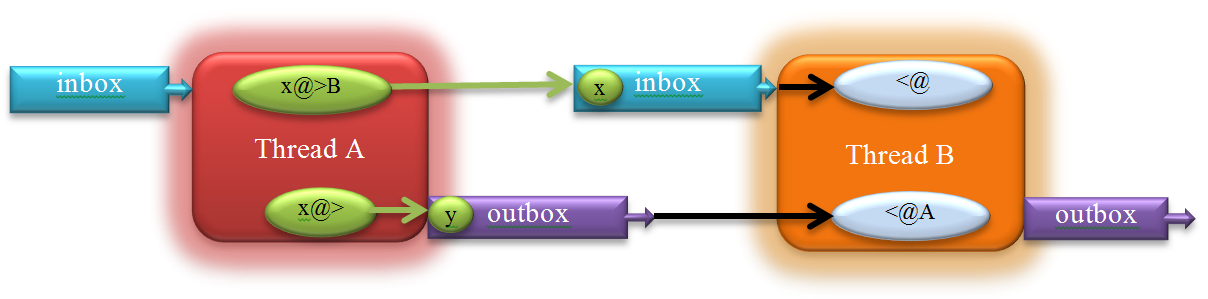
\includegraphics[width=5.75in,height=1.45in]{ub-img/thread-fig1.png}
\end{center}
\vspace{-0.25cm}{\sffamily\bfseries Figure 8-1:}
{\sffamily Inboxes and Outboxes for Thread Communication.}


\subsection*{\texttt{send} and \texttt{receive} operators}

The \texttt{@>} (send) and \texttt{{<}@} (receive) operators communicate
messages containing arbitrary data between threads. The operators support
co-expressions as well, with the same semantics. The send operator has the
syntax

\iconcode{
x @>T
}

\noindent
where \texttt{x} can be any data type, including null, which is equivalent to omitting
it. \texttt{T} refers to a thread to which \texttt{x} is transmitted: \texttt{x}
is placed in \texttt{T}'s inbox.  \texttt{x} can be picked by \texttt{T} using
the receive operator which is presented later.
\texttt{x @> \&main} may be used to send a message to the main thread.
The send operator can also have no destination, as in

\iconcode{
x @>
}

In this case \texttt{x} is sent to no one, instead it is placed in the sender's
outbox. The operator can be read as ``produce \texttt{x}''.  \texttt{x} can then
be picked up later by any thread wanting a value from this sender.  For example
the sender in this case might be a creating prime numbers and placing them in
its outbox to be ready for other threads.

The receive operator is symmetric to send, and takes two forms, with explicit
source or with no source, as follows:

\iconcode{
{<}@T \\
{<}@
}

\noindent
The first case reads ``receive a value from \texttt{T}''; it obtains a value
from \texttt{T}'s outbox. In the prime number example mentioned
above, \texttt{<@T} would be the way to get a prime number produced by
\texttt{T}. \texttt{{<}@} on the other hand reads values directly from the
receiver's inbox.  It reads messages sent explicitly to the thread doing the
receive operation.

Both \texttt{@>} and \texttt{{<}@} can succeed or fail. In the case of
\texttt{{<}@} the operator succeeds and returns a value from the corresponding
queue (inbox/outbox) depending on the operand if the queue is not empty. If the
queue is empty the operation fails directly. In the case of \texttt{@>}, if the
value is placed in the corresponding queue the operation succeeds and returns
the size of the queue. If the queue is full, the send operation fails. The
inbox/outbox for each thread is initialized to have a limited size (it can hold
up to 1024 values by default). This limit can be increased or decreased
depending on the application needs. The limits are useful so that queue sizes do
not explode quickly by default. They also provide an implicit
communication/synchronization as explained later in following sections.  Let us
look at the producer/consumer example again written using the new operators:

\iconcode{
procedure main() \\
\ \ \ p := thread produce() \\
\ \ \ c := thread consume(p) \\
\ \ \ every wait(p {\textbar} c) \\
end \\
\ \\
procedure produce() \\
\ \ \ every !10 @> \ \ \# place values in my outbox \\
end \\
\ \\
procedure consume(p) \\
\ \ \ i := 0 \\
\ \ \ while i {<} 10 do \\
\ \ \ \ \ \ if x := {<}@ p then\ \ \# get values from p \\
\ \ \ \ \ \ \ \ \ i +:= 1 \& write(x) \\
end
}

Each thread has exactly one inbox and one outbox, and each operator call is
mapped to only one of these inboxes or outboxes as seen in Figure 1.  All
messages from all threads coming to thread B in the figure end up in its
inbox. All threads trying to receive messages from A compete on A's outbox. Both
the inbox and the outbox queues are public communications channels, and it is
impossible to distinguish the source of a message if there are several threads
sending messages to the same thread at the same time. Furthermore, if
\texttt{{<}@} has an explicit source like A in Figure 1, it only looks in A's
outbox, and does not see messages from A coming directly to the
inbox. Applications that require the sender's address can attach that
information to messages by building them as records with two fields, one field
for data and the other containing the sender's address. A better approach for
private communications for some applications is the use of lists shared between
the two communicating threads or the use of private communication channels
discussed later in this document.


\subsection*{Inbox/Outbox and the \texttt{Attrib()} function}

As seen in previous sections, communication between threads is done though
inbox/outbox queues which have size limits. The size limit, which defaults to
1024, and the actual size dictate how synchronization is merged with the
communication. The size operator \texttt{*} can be used with a thread to query
its actual outbox size (how many values it contains, not the maximum limit), as
follows:

\iconcode{
outbox\_size := *T
}

But this is only a single attribute for one queue.  To access or change other
queue attributes, a new function \texttt{Attrib()} is introduced.  This function
uses the form \texttt{Attrib(handle, attribcode, value, attribcode, value,
  ...)}. The integer codes used by this function are defined in an include file
\texttt{threadh.icn}. This header file is part of the \texttt{threads} package,
which can be used by a program via

\iconcode{
import threads
}

When values are omitted, \texttt{Attrib()} generally returns attribute
values. To get the size of the outbox (the same as the \texttt{*} operator), the
code is

\iconcode{
outbox\_size := Attrib(T, OUTBOX\_SIZE)
}

\noindent similarly, 

\iconcode{
inbox\_size := Attrib(T, INBOX\_SIZE)
}

\noindent
gets the current size of the inbox. On the other hand

\iconcode{
Attrib(T, INBOX\_LIMIT, 64, OUTBOX\_LIMIT, 32)
}

sets the inbox and outbox size limits to 64 and 32 respectively. The following
table summarizes the available attributes and their meanings.


\bigskip

\begin{flushleft}
\tablehead{}
\begin{supertabular}{m{2.0941598in}m{1.9087598in}m{1.9108598in}}
Attribute &
Meaning &
Read/Write?\\
INBOX\_SIZE &
Number of items in the inbox &
Read Only\\
OUTBOX\_SIZE &
Number of items in the outbox &
Read Only\\
INBOX\_LIMIT &
The maximum number of items allowed in the inbox &
Read/Write\\
OUTBOX\_LIMIT &
The maximum number of items allowed in the outbox &
Read/Write\\
\end{supertabular}
\end{flushleft}


\subsection*{Blocking send and receive}

In many situations senders and receivers generate and consume messages at
different speeds or based on needs. Instead of overloading slow receivers or
busy waiting for slow senders, the two ends of the communication need a
synchronizing mechanism to tell them when to send new messages or when a new
message is available. Two more send and receive operators provide such
functionality, the blocking send operator \texttt{@>{}>} and the blocking
receive operator \texttt{<{}<@}.  These can be used in the same way as
\texttt{@>} and \texttt{{<}@}, except that instead of failing when the operation
cannot be completed, the new operators block and wait until the operation
succeeds. In the simple producer/consumer example, the producer is only
producing 10 values, since the default size of the queue is 1024, using a
blocking send would not make any difference. The consumer however, can make use
of the blocking receive instead of spinning in some cases while the queue is
empty and the original blocking receive just keeps failing.  Take a closer look
at the consumer code again:

\iconcode{
procedure consume(p) \\
\ \ \ i := 0 \\
\ \ \ while i {<} 10 \ do \\
\ \ \ \ \ \ if x := {<}@ p then\ \ \# get values from p \\
\ \ \ \ \ \ \ \ \ i +:= 1 \& write(x) \\
end
}

Using an \texttt{if} statement with \texttt{{<}@} checks whether the operation
succeeds in receiving a value. A blocking receive is more suitable in this case
and it simplifies the loop slightly, since the \texttt{if} can be dropped, and
also the counter is not necessary anymore. The counter was previously necessary
because the loop needs to keep track of how many \texttt{{<}@} were needed to
count to 10. The consumer can be rewritten as

\iconcode{
procedure consume(p) \\
\ \ \# get exactly 10 values from p, block if necessary\\
\ \ \ every !10 do write({<}{<}@ p) \\
end
}

In some cases, a thread might want to use a blocking receive to get values from
a second thread, but it is not willing to block indefinitely; it may do some
other useful work instead of waiting. The \texttt{<{}<@} operator accepts a
timeout parameter to impose a limit on how long to wait for a result before
giving up. Here is how \texttt{<{}<@} would look in this case:

\iconcode{
result := timeout {<}{<}@ \ \ \ \ \# \ get from my inbox
}

or 

\iconcode{
result := timeout {<}{<}@ T\ \ \ \ \# get from T's outbox
}

The timeout operand is a non-negative integer denoting the maximum time to wait
in milliseconds.  Negative integers are treated as a null value, defaulting to
an indefinite blocking receive.  A 0 operand indicates no waiting time,
effectively resulting in a non-blocking receive.  The following table summarizes
the different forms of the send and receive operators and their operands:


\bigskip

\begin{flushleft}
\tablehead{}
\begin{supertabular}{m{0.8920598in}m{0.8643598in}m{4.10186in}}
\centering Operator &
\centering Operands &
\centering\arraybslash Behavior\\
\centering @>\par
\centering (send) &
\centering msg@> &
Place msg in my outbox, fail if the outbox is full\\
 &
\centering msg@>T &
Place msg in T's inbox, fail if T's inbox is full\\
\centering {<}@\par

\centering (receive) &
\centering {<}@ &
get a message from my inbox, fail if the inbox is empty\\
 &
\centering {<}@T &
get a message from T's outbox, fail if T's outbox is empty\\
\centering @{>}{>}\par

\centering (blocking send) &
\centering msg@{>}{>} &
Place msg in my outbox, block if the outbox is full\\
 &
\centering msg@{>}{>}T &
Place msg in my T's inbox, block if the T's inbox is full\\
\centering {<}{<}@\par

\centering (blocking receive) &
\centering {<}{<}@ &
Get a message from my inbox, block if the inbox is empty\\
 &
\centering {<}{<}@T &
Get a message from T's outbox, block if
it is empty\\
 &
\centering n{<}{<}@ &
Get a message from my inbox, block up to n milliseconds
waiting for an inbox message to become available\\
 &
\centering n{<}{<}@T &
Get a message from T's outbox, block up to n
milliseconds waiting for a message to become available there\\
\end{supertabular}
\end{flushleft}

\bigskip

Most applications use only a few of these modes. In a fast sender/slow receiver
application, the sender would block when the queue is full and unblock when the
queue is empty (using \texttt{@>{}>}). The receiver would consume messages from
the queue until it is empty, and then block until there is a new message added
to the queue (\texttt{<{}<@}). For some applications however this communication
scheme might not be optimal, hence many options are provided. The different
options in the table above give the programmer a wide range of control over when
to block or resume a thread based on the availability of data in the
communication queues. This control covers the needs of many applications and
provides simple ways to abstract concurrent programming activities such as load
balancing and efficient use of resources.

\subsection*{Private communication channels}

As mentioned in the previous sections, inbox and outbox communication queues are
visible by all threads all the time. In some scenarios two or more threads need
to communicate with each other without worrying about other threads sending and
receiving messages at the same shared queues. While it is possible to build a
protocol at the application level on top of the inbox and outbox queues to
achieve such behavior, it is simpler and more efficient to have the threads
communicate privately. This kind of communication can be done by sharing a list
between two threads and protecting it by an explicit mutex, or using a
thread-safe list. A more formal way for such communication is to use the
\texttt{channel()} function.

Starting a private communication is similar to a network connection, except that
this connection is taking place between two threads in the same process instead
of two different processes that may be on different machines. A private
communication channel between two threads can be created using the library
procedure \texttt{channel()}.

\texttt{channel()} is part of the \texttt{threads} package, so \texttt{import
  threads} is necessary to use it.  It takes one parameter, which is the thread
with which the connection will be initiated.  If \texttt{channel()} succeeds, it
returns a list representing a communication channel between the two
threads. Representing a bidirectional channel that can be used by the two
threads, given that each thread calls the function \texttt{channel()} with the
other thread as an argument.  Here is an example.

In thread A:

\iconcode{
\ \ \ \ \ \ \ \ chB := channel(B) \ {\textbar} "failed to open a channel with B"
}

In thread B:

\iconcode{
\ \ \ \ \ \ \ \ chA := channel(A) \ {\textbar} "failed to open a channel with A"
}

A channel is a \emph{directional} communication medium.  One thread should use
it as an outbox, and the other should use it as an inbox; only one thread will
send messages over the channel while the other receives them from the other
end. The provided channel can be used with the communication operators (all four
of them) with the same semantics as before. The only difference in this case is
that the right operand is a communication channel instead of a thread.  In the
channel example below, the main thread transmits the consumer's identity to the
producer (\texttt{c @> p}), who receives it via \texttt{c := <{}<@}:

\iconcode{
import threads \\
procedure main() \\
\ \ \ p := thread produce() \\
\ \ \ c := thread consume(p) \\
\ \ \ c @> p \\
\ \ \ every wait(p {\textbar} c) \\
end \\
\ \\
procedure produce() \\
\ \ \ c := {<}{<}@ \\
\ \ \ chC := channel(c) \\
\ \ \ every !10 @> chC \ \ \# place values in channel c \\
end \\
\ \\
procedure consume(p) \\
\ \ \ chP := channel(p) \\
\ \ \ every !10 do write({<}{<}@chP) \\
end
}


\section{Summary}

True concurrency opens up major new application domains for the Unicon language.
More importantly, it enables the language to utilize more than the small
fraction of modern processors utilized by traditional sequential execution. For
example, on a typical quad-core desktop, many applications will be able to get
between 2$\times$ and 4$\times$ the performance of a sequential Unicon program
with relatively minor changes. This is comparable to the speedup typically
delivered by the optimizing compiler.  Some applications will be able to do even
better on processors with more cores.

This document presented Unicon's concurrency facilities from a programmer's
perspective. The implementation and its performance are described in more detail
in [Al-G12]. There are major areas for future work, including GPU- and APU
support, and various forms of implicit concurrency that can be added to the
language.


\section{Part II: Object-oriented Software Development}

\clearpage
\ \bigskip
\clearpage

\chapter{Objects and Classes}

\index{object-oriented programming}Object-oriented programming means
different things to different people. In Unicon, object-oriented
programming starts with encapsulation, inheritance, and polymorphism.
These ideas are found in most object-oriented languages as well as many
that are not object-oriented. This and following chapters
present these ideas and illustrate their use in design diagrams and
actual code. Diagrams and code are
alternative notations by which programmers share their knowledge. This
chapter explores the essence of object-orientation and gives you the
concepts needed before you delve into diagrams and code examples. In
this chapter you will learn:
\begin{itemize}\itemsep0pt
\item How different programming languages support objects in different ways
\item To simplify programs by encapsulating data and code
\item The relationship between objects and program design
\item Draw diagrams that show class names, attributes, and methods
\item Write corresponding code for classes and their methods
\item To create instances of classes and invoke methods on those objects
\end{itemize}

\section{Objects in Programming Languages}

Object-oriented programming can be done in any language, but some
languages make it easier than others. Support for objects should not
entail strange syntax or programs that look funny in a
heterogeneous desktop-computing environment. \index{Smalltalk}Smalltalk
has these problems. C++ avoids these programs, but its low-level
machine-orientation is less than ideal as an algorithmic
notation usable by non-experts. \index{Java}Java offers a simple object
model and familiar syntax. The advantages
Unicon has over Java are fundamentally higher-level built-in types,
operations, and control structures.

Many object-oriented languages require that \textit{everything} be done
in terms of objects, even when objects are not appropriate. Unicon
provides objects as just another tool to aid in the writing of
programs, especially large ones. Icon already provides a powerful
notation for expressing a general class of algorithms. The purpose of
object-orientation is to enhance that notation, not to get in the way
of it.

Icon does not support user-defined objects, although its built-in types
have nice object-like encapsulation and polymorphism properties.
Unicon's object-oriented facilities descend from a
package for Icon called \index{Idol}Idol. In Idol, a preprocessor
implemented objects with no support from the underlying Icon runtime
system. In contrast, Unicon has support for objects built-in to the
language. This simplifies the notation and improves the performance of
object-related computations.

Object-orientation adds several general concepts into procedure-based
programming. The single overriding reason for \index{object-oriented
programming}object-oriented programming is to reduce complexity in
large programs. Simple programs can be written easily in any language.
Somewhere between the 1,000-line mark and the 10,000-line mark most
programmers can no longer keep track of their entire program at once.
By using a very high-level programming language, fewer lines of code
are required; a programmer can write perhaps ten times as large a
program and still be able to keep track of things.

As programmers write larger and larger programs, the benefit provided by
\index{very high-level language}very high-level languages does not keep
up with program complexity. This obstacle has been labeled the
"software crisis," and object-oriented
programming is one way to address this crisis. In short, the goals of
object-oriented programming are to reduce the complexity of coding
required to write very large programs and to allow code to be
understood independently of the context of the surrounding program. The
techniques employed to achieve these goals are discussed below. 

A second reason to consider object-oriented programming is that the
paradigm fits certain problem domains especially well, such as
simulation, and graphical user interfaces. The first well-known
object-oriented language, \index{Simula67}Simula67, certainly had the
domain of simulation in mind. The second pioneering object-oriented
language, Smalltalk, popularized fundamental aspects of bitmapped
graphical user interfaces that are nearly universal today. Three
decades of experience with object-oriented techniques has led many
practitioners to conclude that the concepts presented below are very
general and widely applicable, but not all problems fit the
object-oriented mold. Unicon advocates the use of objects, but this is
a suggestion, not a rule. 

\subsection{Encapsulation}

The primary concept advocated by object-oriented programming is the
principle of \index{encapsulation}encapsulation. Encapsulation is the
isolation, in the source code that a programmer writes, of a data
representation and the code that manipulates the data representation.
In some sense, encapsulation is an assertion that no other routines in
the program have {\em side-effects\/} with
respect to the data structure in question. It is easier to reason about
encapsulated data because all of the source code that could affect that
data is immediately present with its definition. 

Encapsulation does for data structures what the procedure does for
algorithms: it draws a line of demarcation in the program source code.
Code outside this boundary is irrelevant to
the code that is inside, and vice versa. Communication across the
boundary occurs through a public interface. An encapsulated
data structure is called an object. Just as a set of named variables called
parameters is the interface between a procedure and the
code that uses it, a set of named procedures called methods comprises
the interface between an object and the code that uses it. 

This textual definition of encapsulation as a property of program source
code accounts for the fact that good programmers can write encapsulated
data structures in any language. The problem is not capability, but
verification. To verify encapsulation some languages require
programmers to specify the visibility of every piece of information in
each data structure as {\em public\/} or
{\em private\/}. There are even multiple forms of
privacy (semi-private?). Unicon instead stresses simplicity. 

\subsection{Inheritance}

In large programs, the same or nearly the same data structures are used
over and over again for myriad different purposes. Similarly,
variations on the same algorithms are employed by structure after
structure. To minimize redundancy, techniques are needed to support
code sharing for both data structures and algorithms. Code is shared by
related data structures through a programming concept called
\index{inheritance}inheritance. 

The basic premise of inheritance is simple: when writing code for a data
structure similar to a structure that is already written,
specify the new structure by giving the differences between it and
the old structure, instead of copying and modifying the old
structure's code. There are times when the
inheritance mechanism is not useful, such as if the two data structures
are more different than they are similar, or if they are simple enough
that inheritance would only confuse things, for example. 

Inheritance addresses multiple programming problems found at
different conceptual levels. The most obvious software engineering
problem it solves might be termed enhancement. During the development
of a program, its data structures may require extension via new state
variables or new operations or both; inheritance is especially useful
when both the original structure and the extension are used by the
application. Inheritance also supports simplification, or the reduction
of a data structure's state variables or operations.
Simplification is analogous to \index{argument culling}\textit{argument
culling}\textit{,} an idea from lambda calculus (don't
worry if this sounds like Greek to you), in that it describes a logical
relation between structures. In general, inheritance may be used in
source code to describe any sort of relational hyponymy, or special
casing. In Unicon the collection of all inheritance relations defines a
directed (not necessarily acyclic) graph. 

\subsection{Polymorphism}

\index{polymorphism}From the perspective of the writer of related data
structures, inheritance provides a convenient method for code sharing,
but what about the code that uses objects? Since objects are
encapsulated, that code is not dependent upon the internals of the
object at all, and it makes no difference to the client code whether
the object in question belongs to the original class or the inheriting
class. 

We can make a stronger statement. Due to encapsulation,
different executions of code that uses objects to implement an
algorithm may operate on objects that are not
related by inheritance at all. Such code can utilize any objects that
implement the operations that the code invokes. This facility is called
polymorphism, and such algorithms are called generic. This feature is
found in many non-object-oriented languages; in object-oriented
languages it is a natural extension of encapsulation. 

\section{Objects in Program Design}

\index{program design}Another fundamental way to think about objects is
from the point of view of software design. During program design,
objects are used to model the problem domain. The different kinds of
objects and relationships between objects capture fundamental
information that organizes the rest of the program's
design and implementation. Program design includes several other
fundamental tasks such as the design of the user interface, or
interactions with external systems across a network. Additional kinds
of modeling are used for these tasks, but they all revolve around the
object model.

For small, simple, or well-understood software projects, a prose description
may be all the documentation that is needed. The Unified Modeling Language
(\index{UML}UML) is a notation for building software models of larger software
systems for which a prose description alone would be inadequate. It was
invented by Grady Booch, Ivar Jacobson, and James Rumbaugh. In UML, software
models document the purpose and function of a software system.
The advantage of a model is that it conveys
information that is both more precise and more readily understood than
a prose description. UML is used during multiple phases of the software
lifecycle. UML defines several kinds of diagrams, of which we will only
consider four in this book.

\begin{itemize}
\item \textbf{Use case diagrams} show the organization of the
application around the specific tasks accomplished by different users.
\item \textbf{Class diagrams} show much of the static structure of the
application data.
\item \textbf{Statechart diagrams} model dynamic behavior of systems
that respond to external events, including user input.
\item \textbf{Collaboration diagrams} model interactions between
multiple objects
\end{itemize}
These diagrams describe key aspects of many categories of software
applications. The reader should consult the UML Notation Guide and
Semantics documents for a complete description of UML. A good
introduction is given in \textit{UML Toolkit}, by Hans-Erik Eriksson
and Magnus Penker (1998).

A typical application of UML to a software development project uses
these diagrams in sequence. You start by constructing
use case diagrams and detailed descriptions of the different kinds of
users and tasks performed using the system. Then develop class diagrams
that capture the relationships between different kinds of objects
in the system. Finally, construct statechart and
collaboration diagrams as needed to describe the sequences of events
that can occur and the corresponding operations performed by various
objects in response to those events.

Use case and statechart diagrams are important, but their purpose is
to elaborate on an object model described in class diagrams. For this
reason, class diagrams are
presented first, along with the corresponding programming
concepts. Use case diagrams, statecharts, and collaboration diagrams
are discussed in chapter 12.

\section{Classes and Class Diagrams}

Classes are user-defined data types that model the information and
behavior of elements in the application domain. In Unicon they are
records with associated procedures, called methods. Instances of these
special record types are called objects.  But the language constructs
originated from a need to model application domain concepts, so it is
appropriate to introduce them from that perspective.

Modeling a software system begins with identifying things
that are in the system and specifying how they are related. A class
diagram shows a static view of relationships between the kinds of
elements that occur in the problem domain. A class diagram is a
data-centric, object-centric model. In contrast, a
user-centric view is provided by use cases. \index{class!diagrams}Class
diagrams have several basic components.

Classes are represented by rectangles. A
{\em class\/} denotes a concept of the
application domain that has state information (depicted by named
\index{attribute!class}\textit{attributes}) and/or behavior (depicted
by named \index{operations}operations, or \textit{methods}) significant
enough to be reflected in the model. Inside the rectangle, lines
separate the class name and areas for attributes and operations. Figure
9-1 shows an example class.

\bigskip

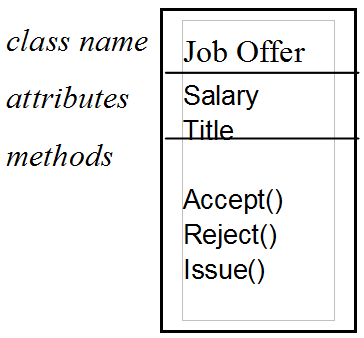
\includegraphics[width=2.3in,height=1.8in]{ub-img/umlclass.png} 

{\sffamily\bfseries Figure 9-1:}
{\sffamily Class Job Offer has two Attributes and Three Methods}

\bigskip

Classes in an object model are
implemented using programming language classes, which are described in
the next section. The degree of separation between the notion of a
class in the model and in the implementation depends on the programming
language. In the case of Unicon, the separation is minimal, because
built-in types such as lists and tables take care of almost all data
structures other than those introduced specifically to model
application domain elements. In the case of C++ or \index{Java}Java,
many additional implementation artifacts typically have to be
represented by classes.

The same class can appear in many class diagrams to capture all of its
relationships with other classes. Different diagrams may show different
levels of detail, or different aspects (projections) of the class
relevant to the portion of the model that they depict. In the course of
modeling it is normal to start with few details and add them gradually
through several iterations of the development process. Several kinds of
details may be added within a class. Such details include:

\begin{itemize}
\item The \index{visibility!within class}\textit{visibility} of
attributes and operations. A plus sign (+) before the attribute name
indicates that the attribute is \index{public}public and may be
\index{reference}referenced in code external to the class. A minus sign
(-) before the attribute name indicates that the attribute is
\index{private}private and may not be referenced in code outside the
class.
\item Types, initial values, and properties of attributes
\item Static properties of the class that will not be relevant at
run-time
\end{itemize}
Attribute names may be suffixed with a colon and a type, an equal sign
and a value, and a set of properties in curly braces. Figure 9-2 shows
two very different levels of detail for the same class. Each level of
detail is appropriate in different contexts.

\bigskip

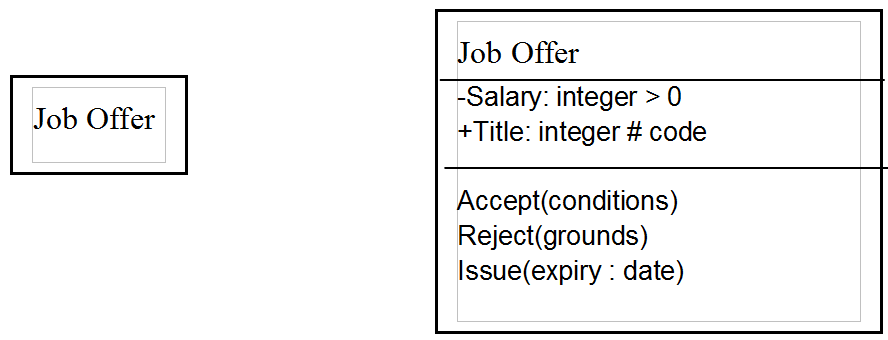
\includegraphics[width=4in,height=1.8in]{ub-img/lodetail.png} 

{\sffamily\bfseries Figure 9-2:}
{\sffamily A Class is Drawn with Different Levels of Detail in
 Different Diagrams}

\bigskip

You can draw rectangles with names of classes inside them all day, but
unless they say something about program organization, such diagrams
serve little purpose. The main point of drawing a class diagram is not
the classes; it is the relationships between classes that are required
by the model. These relationships are called
\index{association}\textit{associations}. In a class diagram,
associations are lines that connect classes. Accompanying annotations
in the diagram convey relevant model information about the
relationships. The details of associations and their implementation are
described in chapter 10.

\section{Declaring Classes}

\index{class!declaration}In Unicon program code, the syntax of a class
is: 

\iconcode{
class foo(attribute1, attribute2, attribute3, ...) \\
\>   \# procedures (methods) to access class foo objects \\
\ \\
\# code to initialize class foo objects \\
end
}

\noindent
The procedures that manipulate class objects are called
\index{method}\textit{methods}. Methods define a
class' interface from the rest of the program. The
syntax of a method like a procedure: 

\iconcode{
method bar(param1, param2, param3, ...) \\
\>   \# Unicon code that may access fields of a class foo object \\
end
}

Execution of a class method is always associated with a given object of
that class. The method has access to an implicit
\index{variable!implicit}\index{variable}variable called
\index{self}\texttt{self} that is a record containing fields whose
names are the attributes given in the class declaration. Fields from
the \texttt{self} variable are directly accessible by name. In addition
to methods, classes may also contain regular procedure, global, and
record declarations; such declarations have the standard semantics and
exist in the global name space. 

\section{Object Instances}

Like records, \index{instances!class object}instances of a class type
are created with a \index{constructor!class}constructor function whose
name is that of the class. Instances of a class are called objects, and
behave similar to records. The fields of an instance generally
correspond directly to the class attributes. Fields may be initialized
explicitly in the constructor in exactly the same way as for records.
For example, after defining a \texttt{class foo(x, y)} one may write: 

\iconcode{
procedure main() \\
\>   f := foo(1, 2) \\
end
}

In this case \texttt{x} would have the value \texttt{1}, and \texttt{y}
would have the value \texttt{2}, the same as for a record
type. The fields of an object do not have to be initialized by a
parameter passed to the class constructor. Many constructors initialize
objects' fields to some standard value. In this case,
the class declaration includes an \index{initially}\texttt{initially}
section after its methods are defined and before its end. An
\texttt{initially} section is just a special method that is invoked
automatically by the system when it creates each instance of the class.

An \texttt{initially} section begins with the word
\texttt{initially} and an optional parameter list, followed by lines of
code that are executed when an object of that class is constructed.
These lines can assign values to the attributes of the object
being created.

For example, suppose you want an enhanced table type that permits
sequential access to elements in the order they are inserted into the
table. You can implement this using a combination of a list and a
table, both of which would be initialized to the appropriate empty
structure: 

\iconcode{
class taque(L, T) \# pronounced "taco" \\
\>   \# methods to manipulate taques, \\
\>   \# e.g. insert, index, foreach... \\
initially \\
\>   L := [ ] \\
\>   T := table() \\
end
}

\noindent
In such a case you can create objects without including arguments to the
constructor: 

\iconcode{
procedure main() \\
\ \ \ mytaque := taque() \\
end
}

In the absence of an \texttt{initially} section, missing arguments to a
constructor default to the null value. Together with an
\texttt{initially} section, the class declaration looks like a
procedure that constructs objects of that class. You can
write classes with some fields that are initialized explicitly by the
constructor while other fields are initialized automatically in the
\texttt{initially} section. In this case you should either declare the
automatically initialized fields after those initialized in
the constructor, or insert \texttt{\&null} in the positions of the
automatically initialized fields in the constructor. The parameters to
the constructor are exactly in the order they appear in the class
declaration.

This default semantics for constructor parameters is awkward in some
cases, so there is an alternative. The \texttt{initially} section is
really just a special method, and it is allowed to take a parameter
list just like any other method. When an initially section includes a
parameter list, no implicit initialization of objects'
fields is performed. This frees the constructor from having the same
number and order of parameters as the declared class fields. In the
following class, the third field is initialized from constructor
parameter \texttt{x}, overriding the default behavior of initializing
fields in the declared order. This capability becomes important in
large classes with many fields.

\iconcode{
class C(a, b, c) \\
initially(x) \\
\>   c := x \\
end
}

\section{Object Invocation}

Once you have created an object with a class constructor, you manipulate
the object by invoking its class methods. Since objects are
both procedures and data, object \index{invocation!object
method}invocation is a combination of a procedure call and a record
access. The syntax is

\iconcode{
\>   object . methodname ( arguments )}

If an object's class is known, object methods can also
be called using a normal procedure call. This allows object oriented
Unicon code to be called from Icon. Called as a procedure, the name of
a method is prefixed with the class name and an underscore character.
The object itself is always the first parameter passed to a method. In
the absence of inheritance (discussed in the next chapter) if
\texttt{x} is an object of class \texttt{C},
\texttt{x.method(arguments)} is equivalent to \texttt{C\_method(x,
arguments)}.

Although object methods can be called using procedure calls, the field
operator has the advantage that it handles inheritance and polymorphism
correctly, allowing algorithms to be coded generically using
polymorphic operations. Generic algorithms use any objects whose class
provides the set of methods used in the algorithm. Generic code is less
likely to require change when you later enhance the program, for
example adding new \index{subclass}subclasses that inherit from
existing ones. In addition, if class names are long, the field syntax
is considerably shorter than writing out the class name for the
invocation. Using the taque example: 

\iconcode{
procedure main()\\
\>   mytaque := taque() \\
\>   mytaque.insert("greetings",
"hello") \\
\>   mytaque.insert(123) \\
\>   every write(mytaque.foreach()) \\
\>   if mytaque.index("hello") then 
        write(", world") \\
end
}

For object-oriented purists, using the field operator to invoke an
object's methods in this manner is the only way to
access an object. In Unicon, visibility issues such as
``public'' and ``private'' are addressed in an
application's design and documentation. A good
starting point is to consider all fields
``private'' and all methods ``public''. Nevertheless, an object is just a
kind of record, complete with record-style field access.

Direct external access to an object's data fields using
the usual field operator is not good practice, since it violates the
principle of encapsulation. Within a class method, on the other hand,
access to an object's attributes is expected. The
implicit object named \texttt{self} is used under the covers, but
attributes and methods are referenced by name, like other variables.
The taque insert method is thus: 

\iconcode{
method insert(x, key) \\
\>   /key := x \\
\>   put(L, x) \\
\>   T[key] := x \\
end
}

The \texttt{self} object allows field access just like a record, as well
as method invocation like any other object. Using the \texttt{self}
variable explicitly is rare.

\section{Comparing Records and Classes by Example}

The concepts of classes and objects are found in many programming
languages. The following example illustrates Unicon's object model
and provides an initial impression of these
concepts' value. To motivate Unicon's OOP
constructs, our example contrasts conventional Icon
code with object-oriented code that implements the same behavior.

\subsection{Before objects}

Suppose you are writing some text-processing application such as a text
\index{editor}editor. Such applications need to be able to process
structures holding the contents of various text files. You might begin
with a simple structure like the following: 

\iconcode{
record buffer(filename, text, index)}

\noindent
where \texttt{filename} is a string, \texttt{text} is a list of strings
corresponding to lines in the file, and \texttt{index} marks
the current line at which the buffer is being processed. Icon record
declarations are global; in principle, if the above declaration needs
to be changed, the entire program must be rechecked. A devotee of
structured programming would write procedures to read the buffer
in from a file; write it out to a file; examine, insert and delete
individual lines; and so on. These procedures, along with the record
declaration given above, can be placed in their own source file
(\texttt{buffer.icn}) and understood independently of the program(s) in
which they are used. Here is one such procedure: 

\iconcode{
\# read a buffer in from a file \\
procedure read\_buffer(b) \\
\>   f := open(b.filename) {\textbar} fail \\
\>   b.text := [ ] \\
\>   b.index := 1 \\
\>   every put(b.text, !f) \\
\>   close(f) \\
\>   return \\
end
}

There is nothing wrong with this example; in fact its similarity to the
object-oriented example that follows demonstrates that a good, modular
design is the primary effect encouraged by \index{object-oriented
programming}object-oriented programming. Using a separate source file
to contain a record type and those procedures that operate on the type
allows an Icon programmer to maintain a voluntary encapsulation of that
type. 

\subsection{After objects}

Here is part of the same buffer abstraction coded in Unicon. This
example lays the groundwork for some more substantial techniques to
follow. Methods are like procedures that are always called in reference
to a particular object (a class instance).

\iconcode{
class buffer(filename, text, index) \\
\>   \# read a buffer in from a file \\
\>   method read() \\
\>   \ \ \ f := open(filename) {\textbar} fail \\
\>   \ \ \ text := [ ] \\
\>   \ \ \ index := 1 \\
\>   \ \ \ every put(text, !f) \\
\>   \ \ \ close(f) \\
\>   \ \ \ return \\
\>   end \\
\>   \# ...additional buffer operations, including method erase() \\
initially \\
\>   if {\textbackslash}filename then read() \\
end
}

This example does not illustrate the full object-oriented style, but it
is a start. The object-oriented version offers encapsulation and
polymorphism. A separate name space for each class's
methods allows shorter names. The same method name, such as
\texttt{read()}, can be used in each class that
implements a given operation. This notation is more concise than is
possible with procedures, and it enables an algorithm to
work on objects of any class that implements the operations required by
that algorithm. 

Consider the initialization of a new buffer. Constructors allow the
initialization of fields to values other than \texttt{\&null}. In the
example, the \texttt{read()} method is invoked if a filename is
supplied when the object is created. This can be simulated using
records by calling a procedure after the record is created; the value
of the \index{constructor!record}constructor is that it is automatic.
The programmer is freed from the responsibility of remembering to call
this code everywhere objects are created in the client program(s). This
tighter coupling of \index{memory allocation}memory allocation and its
corresponding initialization removes one more source of program errors,
especially on multi-programmer projects. 

The preceding two paragraphs share a common theme:
the net effect is that each piece of data is made responsible for its
own behavior in the system. Although this example dealt with simple
line-oriented text files, the same methodology applies to more abstract
entities such as the components of a
\index{compiler}compiler's grammar.

The example illustrates an important scoping issue. Within class
buffer, method \texttt{read()} makes the regular built-in
function \texttt{read()} inaccessible! Beware of such
conflicts. It would be easy to capitalize the method name to
eliminate the problem. If renaming the method is not an option, as a
last resort you could get a reference to the built-in function
\texttt{read()}, even within method \texttt{read()}, by calling
\texttt{proc("read", 0)}. The function
\texttt{proc()} converts a string to a procedure; supplying a second
parameter of 0 tells it to skip scoping rules and look for a built-in
function by that name.

\section{Summary}

Classes are global declarations that define a record data type and a
set of procedures (methods) that operate on that type. Class instances,
called objects, are normally manipulated solely by calling
the class' methods; such object privacy is a matter of
design, documentation, and
convention. All methods execute within an
object of interest, whose fields and methods are visible
without the record dot notation, in a
class scope that is introduced in between the local and global scopes.




\bigskip


\clearpage
\ \\ \bigskip

\chapter{Inheritance and Associations}

Relationships between classes are depicted in UML class diagrams by
lines drawn between two or more class rectangles. One of the most
important relationships between classes describes the situation when
one class is an extension or minor variation of another class: this is
called generalization, or \textit{inheritance}. Most other
relationships between classes are really relationships between those
classes' \index{instance}instances at run-time; these
relationships are called \textit{associations}. This chapter starts
with inheritance, and then describes a variety of associations.
In this chapter you will learn how to:
\begin{itemize}\itemsep0pt
  \item Define a new class in terms of its differences from an existing class
  \item Compose aggregate classes from component parts.
  \item Specify new kinds of associations
  \item Supply details about the roles and number of objects in an association
  \item Use structure types from Chapter 2 to implement associations
\end{itemize}

\section{Inheritance}

In many cases, several classes of objects are very similar. In
particular, many classes arise as enhancements of classes that have
already been defined. Enhancements might consist of added fields, added
methods, or both. In other cases a class is just a special case of
another class. For example, if you have a class
\texttt{fraction(numerator, denominator)}, you could define class
\texttt{inverses(denominator)} whose behavior is identical to that of a
fraction, but whose numerator is always 1. 

Both of these ideas are realized with the concept of
\index{inheritance}inheritance. When the definition of a class is best
expressed in terms of the definition of another class or classes, we
call that class a \index{subclass}\textit{subclass.} The class or
classes from which a subclass obtains its definition are called
\index{superclass}\textit{superclass}\textit{es}. The logical relation
between the subclass and superclass is called \textit{hyponymy}. It
means an object of the subclass can be manipulated just as if it were
an object of one of its defining classes. In practical terms it means
that similar objects can share the code that manipulates their fields.

Inheritance appears in a class diagram as a line between classes with an
arrow at one end. The arrow points to the superclass, the source of
behavior inherited by the other class. Consider Figure 10-1, in which
an offer of a salaried appointment is defined as one kind of job offer.
The attributes (\texttt{salary}, \texttt{title}) and methods
(\texttt{Accept()} and \texttt{Reject()}) of class JobOffer are
inherited by class SalariedAppointment, and do not need to be repeated
there. A new attribute (term) is added in \texttt{SalariedAppointment}
that is not in \texttt{JobOffer}.

\begin{center}
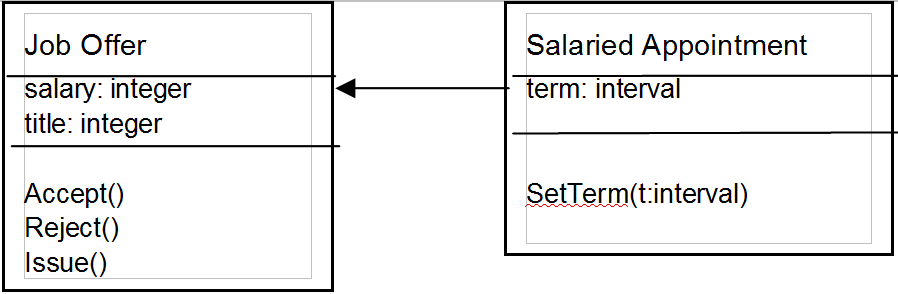
\includegraphics[width=4.05in,height=1.52in]{ub-img/subclass.png} 

{\sffamily\bfseries Figure 10-1:}
{\sffamily A Salaried Appointment is a subclass of a Job Offer}
\end{center}

\noindent
The syntax of a subclass is 

\iconcode{
class \textit{classname} \textit{superclasses} (\textit{attributes}) \\
\>   \textit{methods} \\
{\sffamily\itshape
initially\_section} \\
end
}

Where \texttt{\textit{superclasses}} is an optional list of class names
separated by colons, \texttt{\textit{attributes}} is an optional list
of \index{variable}variable names separated by commas,
\texttt{\textit{methods}} is an optional list of declarations for the
class methods, and the \texttt{\textit{initially\_section}} is optional
initialization code for the class \index{constructor}constructor. \ For
example

\iconcode{
class SalariedAppointment : JobOffer (term) \\
\>   method SetTerm(t : interval) \\
\>   \ \ \ term := t \\
\>   end \\
initially \\
\>   /term := "unknown term" \\
end
}

As you can see, a subclass declaration is identical to a regular class,
with the addition of one or more superclass names, separated by colons.
The meaning of this declaration is the subject of the next section. 

\subsection{Inheritance semantics}

\index{inheritance!semantics}There are times when a new class might best
be described as a combination of two or more classes. Unicon classes
may have more than one superclass, separated by colons in the class
declaration. This is called multiple inheritance.

Subclasses define a record type consisting of the field names of the
subclass itself and all its superclasses. The subclass has associated
methods consisting of those in its own body, those in the first
superclass that were not defined in the subclass, those in the second
superclass not defined in the subclass or the first superclass, and so
on. In ordinary single-inheritance, this adding of fields and methods
follows a linear bottom-up visit of each superclass,
followed in turn by its parent superclass. 

When a class has two or more superclasses, the search generalizes from a
linear sequence to an arbitrary \index{tree}tree, directed acyclic
\index{graph}graph, or full graph traversal. 
\index{inheritance!multiple}Multiple inheritance adds fields and
methods in an order defined by a depth-first traversal of the parent
edges of the superclass graph. Think of the second and following
superclasses in the
multiple inheritance case as adding methods and fields only if the
single-inheritance case (following the first superclass and all its
parents) has not already added a field or method of the same name. 

{\sffamily\bfseries
Warning}

{\sffamily
Care should be taken employing multiple inheritance if the two parent
classes have any fields or methods of the same name! }

Fields are initialized by parameters to the constructor or by the
class \texttt{initially} section, which is a method and is
inherited in the normal way. It is common for a subclass \texttt{initially}
section to call their superclasses'
\texttt{initially} sections, for example:

\iconcode{
class sub : A : B(x) \\
initially \\
\>   x := 0 \\
\>   A.initially() \\
\>   B.initially() \\
end
}

\noindent
It is also common to have some attributes initialized by parameters, and
assign others in the \texttt{initially} section. For example, to define a
class \texttt{inverse} (for numbers of the form 1 / \textit{n}) in terms
of a class \texttt{fraction(numerator, denominator)} one can write: 

\iconcode{
class inverse : fraction (denominator) \\
initially \\
\>   numerator := 1 \\
end
}

Objects of class inverse can be manipulated using all the methods
defined in class fraction; the code is actually shared by both classes
at runtime. 

Viewing inheritance as the addition of superclass elements not found in
the subclass is the opposite of the more traditional object-oriented
view that a subclass is an \index{instance!superclass}instance of the
superclass as augmented in the subclass definition.
Unicon's viewpoint adds quite a bit of leverage, such
as the ability to define classes that are subclasses of each other.
This feature is described further below. 

\subsection{Invoking superclass operations}

\index{superclass!operations}When a \index{subclass}subclass defines a
method of the same name as a method defined in the superclass,
invocations on subclass objects execute the
subclass' version of the
\index{method!overriding}method. This can be overridden by explicitly
including the superclass name in the invocation:

\iconcode{
\>   object\$superclass.method(parameters)}

This facility allows the subclass method to do any additional work
required for added fields before or after calling an appropriate
superclass method to achieve inherited behavior. The result is
frequently a chain of inherited method invocations. 

Since initially sections are methods, they can invoke superclass
operations including superclass initially sections. This allows a chain
of initially sections to be specified to execute in either
subclass-first or superclass-first order, or some mixture of the two. 

\subsection{Inheritance examples}

Several inheritance examples follow from the \texttt{buffer}
example from Chapter 9. Suppose the program does more than
edit text\index{editor}, it has a word-associative
dictionary, bibliography, spell-checker, and thesaurus. These
features can be implemented using the table type.
The contents vary, but they all use string
keyword lookup. As external data, the databases can be stored in text
files, one entry per line, with the keyword at the beginning. The
format of the rest of the line varies from database to database.

Figure 10-2 shows a class diagram with subclasses derived from
\texttt{buffer}. A class \texttt{buftable} refines the
buffer class, adding support for random access. Other classes are
defined as subclasses of \texttt{buftable}. The implementation of these
classes is given below.


\begin{center}
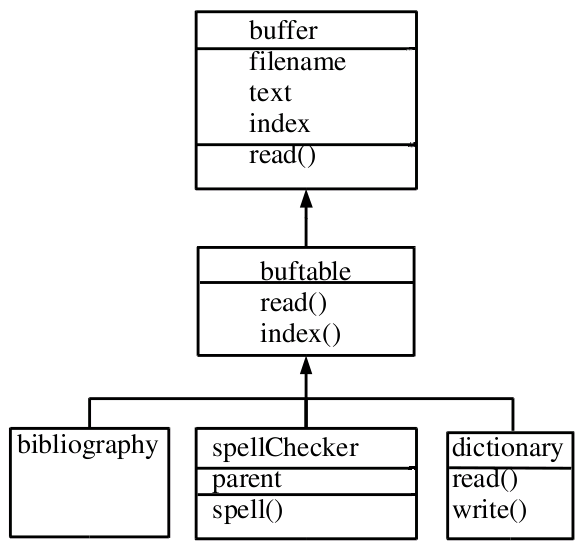
\includegraphics[width=3.24in,height=2.95in]{ub-img/ub-img43.png}
\linebreak
{\sffamily\bfseries Figure 10-2: Some Subclasses of the Buffer Class}
\end{center}

\bigskip

Although all these types of data are different, the code used to read
the data files can be shared, as well as the initial construction of
the tables. In fact, since we are storing our data one entry per line
in text files, we can use the code already written for buffers to do
the file I/O itself. 

\iconcode{
class buftable : buffer() \\
\ \ method read() \\
\>   \ self.buffer.read() \\
\>   \ tmp := table() \\
\>   \ every line := !text do \\
\>   \ \ \ line ? \{ tmp[tab(many(\&letters))] := line {\textbar} fail
\} \\
\>   \ text := tmp \\
\>   \ return \\
\ \ end \\
\ \ method index(s) \\
\>   \ return text[s] \\
\ \ end \\
end
}

This concise example shows how little must be written to achieve data
structures with vastly different behavioral characteristics, by
building on code that is already written. The superclass
\texttt{read()} operation is one important step of the subclass
\texttt{read()} operation. This technique is common enough to have a
name: it is called \textit{method
}\index{method!combination}\textit{combination} in the literature. It
allows you to view the subclass as a transformation of the superclass.
The \texttt{buftable} class is given in its entirety, but our code
sharing example is not complete: what about the data structures
required to support the databases themselves? They are all variants of
the \texttt{buftable} class, and a set of possible implementations
follow. Note that the formats presented are designed to illustrate code
sharing; clearly, an actual application might make different choices. 

\paragraph{Bibliographies}
Bibliographies might consist of a keyword followed by an uninterpreted
string of information. This imposes no additional structure on the data
beyond that imposed by the \texttt{buftable} class. An example keyword
would be Jeffery99. 

\iconcode{
class bibliography : buftable() \\
end
}

\paragraph{Spell-checkers}
The database for a spell-checker might be a list of words, one per
line, the minimal structure required by the \texttt{buftable} class.
Some classes introduce new terminology rather
than to define a new data structure. This example introduces a lookup
operation that can fail, for use in tests. In addition, since many
spell-checking systems allow user definable dictionaries in addition to
their central database, \texttt{spellChecker} objects may chain
together for the purpose of looking up words. 

\iconcode{
class spellChecker : buftable(parent) \\
\ \ method spell(s) \\
\>   \ return {\textbackslash}text[s] {\textbar}
({\textbackslash}parent).spell(s) \\
\ \ end \\
end
}

\paragraph{Dictionaries}
Dictionaries are slightly more involved. Each entry might consist of a
part of speech, an etymology, and an arbitrary string of uninterpreted
text comprising a definition for that entry, separated by semicolons.
Since each such entry is itself a structure, a sensible decomposition
of the dictionary structure consists of two classes: one that manages
the table and external file I/O, and one that handles the manipulation
of dictionary entries, including their decoding and encoding as
strings. 

\iconcode{
class dictionaryentry(word, partofspeech, etymology, definition) \\
\ \ \# decode a dictionary entry into its components \\
\ \ method decode(s)  \\
\>   \ s ? \{ \\
\>   \ \ \ word \ \ \ \ \ \ \ \ :=
tab(upto(';')) \\
\>   \ \ \ move(1) \\
\>   \ \ \ partofspeech :=
tab(upto(';')) \\
\>   \ \ \ move(1) \\
\>   \ \ \ etymology \ \ \ :=
tab(upto(';')) \\
\>   \ \ \ move(1) \\
\>   \ \ \ definition \ \ := tab(0) \\
\>   \ \} \\
\ \ end \\
\ \ method encode() \ \# encode a dictionary entry into a string \\
\>   \ return word {\textbar}{\textbar} ";"
{\textbar}{\textbar} partofspeech {\textbar}{\textbar}
";" {\textbar}{\textbar}
 etymology {\textbar}{\textbar}
";" {\textbar}{\textbar} definition \\
\ \ end \\
initially \\
\ \ if /partofspeech then \{ \\
\>   \ \# constructor was called with a single string argument \\
\>   \ decode(word) \\
\>   \ \} \\
end \\
\ \\
class dictionary : buftable() \\
\ \ method read() \\
\>   \ self.buffer.read() \\
\>   \ tmp := table() \\
\>   \ every line := !text do \\
\>   \ \ \ line ? \{ tmp[tab(many(\&letters))] := dictionaryentry(line)
{\textbar} fail \} \\
\>   \ text := tmp \\
\ \ end \\
\ \ method write() \\
\>   \ f := open(filename, "w") {\textbar}
fail \\
\>   \ every write(f, (!text).encode) \\
\>   \ close(f) \\
\ \ end \\
end
}

\paragraph{Thesauri}
Although an oversimplification, one might conceive of a thesaurus as a
list of entries, each of which consists of a comma-separated list of
synonyms followed by a comma-separated list of antonyms, with a
semicolon separating the two lists. Since the code for such a structure
is nearly identical to that given for dictionaries above, we omit it
here (you might start by generalizing class \texttt{dictionaryentry} to
handle arbitrary strings organized as fields separated by semicolons). 

\subsection{Superclass cycles and type equivalence}

In many situations, there are several ways to represent the same
abstract type. Two-dimensional points might be represented by
\index{Cartesian coordinates}Cartesian coordinates x and y, or
equivalently by radial coordinates expressed as a distance d and angle
r given in \index{radian}radians. If one implements classes
corresponding to these types there is no reason one of them should be
considered a subclass of the other; they are interchangeable and
equivalent.

In Unicon, expressing this equivalence is simple and direct. In defining
classes \texttt{Cartesian} and \texttt{Radial} we may declare them to
be superclasses of each other: 

\iconcode{
class Cartesian : Radial (x, y) \\
\# code that manipulates objects using Cartesian coordinates \\
end \\
\ \\
class Radial : Cartesian (d, r) \\
\# code that manipulates objects using \index{radial coordinates}radial
coordinates \\
end
}

These superclass declarations make the two types equivalent names for
the same type of object; after inheritance,
\index{instance!class}\index{instance}instances of both classes will
have fields x, y, d, and r, and support the same set of operations. 

Equivalent types each have a unique \index{constructor!class}constructor
given by their class name. Often the differing order of the parameters
used in equivalent types' constructors reflects
different points of view. Although they export the same set of
operations, the actual procedures invoked by equivalent
types' instances may be different. For example, if
both classes define an implementation of a method \texttt{print()}, the
method invoked by a given instance depends on which constructor was
used when the object was created.

If a class inherits methods from one of its equivalent classes, it
is responsible for initializing the state of the fields used by
those methods in its constructor. It is also responsible for
maintaining the state of the inherited fields when its methods make
state changes to its own fields. In the geometric example given above,
for class \texttt{Radial} to use any methods inherited from class
\texttt{Cartesian}, it must at least initialize \texttt{x} and
\texttt{y} explicitly in its constructor from calculations on its
\texttt{d} and \texttt{r} parameters. This added
responsibility is minimized in those classes that treat an
object's state as immutable.

\section{Associations}

An \index{association}association denotes a relationship between classes
that occurs between specific instances of the classes at runtime.
Just as objects are instances of classes, associations
have instances called \index{link!association instance}\textit{links.}
Like objects, links have a lifetime, from the instant
at which the relationship is established to the time at which the
relationship is dissolved. Besides serving to connect two objects,
links may have additional state information or behavior; in the most
general case links can be considered to be objects themselves: special
objects whose primary role is to interconnect other objects.

\subsection{Aggregation}

Inheritance may be the most famous kind of relationship between classes,
but it is not the most indispensable. Many languages that provide
objects do not even bother with inheritance. The composition of
assembly objects from their component parts, on the other hand, is a
truly ubiquitous and essential idea called
\index{aggregation}\textit{aggregation}. The class \texttt{dictionary}
defined in the previous section is a good example of an aggregate
object; its component parts are \texttt{dictionaryentry} objects.

Aggregation is depicted in class diagrams by a line between classes with
a diamond marking the aggregate, or assembly, class. Figure 10-3
shows an aggregate found in the domain of sports, where a team is
comprised of a group of players.

\begin{center}
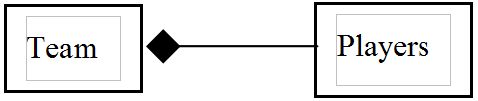
\includegraphics[width=2.52in,height=0.54in]{ub-img/aggregat.png} 

{\sffamily\bfseries Figure 10-3:}
{\sffamily A Team is an Aggregation of Players}
\end{center}

Unlike inheritance, aggregation describes a relationship between
instances at run-time. Different aggregate instances are assembled from
different component part instances. While a given player might play for
different teams over a period of time, at any given instant a player is
normally part of at most one team.

\subsection{User-defined associations}

All the other relationships between classes in \index{UML}UML are left
to the application designer to specify as custom associations.
User-defined associations are depicted by lines, annotated with the
association name next to the line, midway between the two classes.
Figure 10-4 shows a silly user-defined association that describes a
family relationship called Marriage. For a diagram containing such an
association to be well defined, the semantics of such a relationship
must be specified in external documentation that describes Marriage for
the purposes of the application at hand.

\begin{center}
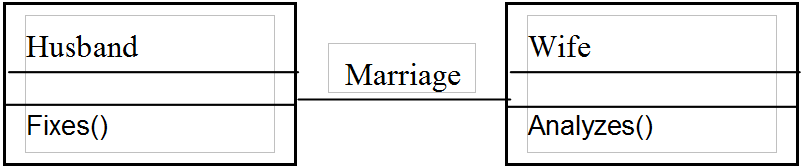
\includegraphics[width=4.8in,height=1.0in]{ub-img/marriage.png} 

{\sffamily\bfseries Figure 10-4:}
{\sffamily A User-Defined Association}
\end{center}

\subsection{Multiplicities, roles, and qualifiers}

Whether they are aggregations or user-defined application domain
relationships, associations are not completely specified until
additional details are determined during program design, such as how
many instances of each type of object may participate in a given
relationship. These additional details appear in canonical positions
relative to the line that depicts the association within a class
diagram.

A \index{multiplicity}\textit{multiplicity} is a number or range that
indicates how many instances of a class are involved in the links for
an association. In the absence of multiplicity information an
association is interpreted as involving just one instance. It normally
appears just below the association line next to the class to which it
applies. Figure 10-5 shows a BasketballTeam that is an aggregate with a
multiplicity of five Players.

\begin{center}
\includegraphics[width=3.78in,height=0.63in]{ub-img/multipcy.png}

{\sffamily\bfseries Figure 10-5:}
{\sffamily Multiplicity of a Basketball Team}
\end{center}

A multiplicity range is expressed as a pair of numbers separated by two
periods, as in 1..3. The value * may be used by itself to indicate that
a link may associate any number (zero or more) of objects. The * value
may also be used in a range expression to indicate no upper bound is
present, as in the range 2..*.

A \index{role}\textit{role} is a name used to distinguish
participants and responsibilities within an association. Roles are
drawn just above or below the association line, adjacent to the class
to which they refer. They are especially useful if a given association
may link multiple instances of the same class in asymmetric
relationships. Figure 10-6 shows a better model of the classes and
roles involved in a Marriage association depicted earlier in Figure
10-4.

\bigskip

\includegraphics[width=4.8in,height=1.2in]{ub-img/roles.png}


{\sffamily\bfseries Figure 10-6:}
{\sffamily Roles in an Association}

\bigskip

A \index{qualifier}\textit{qualifier} is a key value used to
distinguish instances in a link, in lieu of a large
multiplicity that would otherwise be inefficient. For example, a
directory may contain many files, but each one may be directly accessed
by name. A qualifier is drawn as a rectangular association end with the
qualifier key given inside the rectangle. Figure 10-7 shows a
reinterpretation of the basketball aggregation in which the players on
the team are distinguished using a qualifier key named position.


\bigskip

\includegraphics[width=4.8in,height=0.9in]{ub-img/qualifier.png}

{\sffamily\bfseries Figure 10-7:}
{\sffamily Using a Qualifier in lieu of multiplicity}

\subsection{Implementing associations}

Unlike inheritance, which is implemented by the language and resolved at
\index{compile time}compile time, associations involve dynamic
relationships established at runtime, and are implemented by the
programmer...or are they? In the most general case, an association may
be implemented by writing a class whose instances are links between the
related classes' objects. \ In the narrowest special
case, an association can be implemented by adding an attribute in one
class to contain a \index{reference}reference to an object in an
associated class. Much of the value introduced by multiplicity and
qualifier information is to narrow the association semantics down to
what is readily implementable using the built-in structure types
instead of writing classes for them. If an association can be
implemented using a list or table instead of defining a new class, the
resulting code will be smaller and faster.

In all cases, associations will introduce additional fields into the
classes being associated. The following code example implements the
Marriage association from Figure 10-6. For illustration purposes it is
modeled as a one-one relationship at any given point in time. Notice
the intertwining methods in the two classes that establish a
bi-directional relationship. \ Error checking is left as an exercise
for the reader.

\iconcode{
class Man(wife) \\
\>   method Marry(w) \\
\>   \ \ \ wife := w \\
\>   \ \ \ if not (self === w.husband) then w.Marry(self) \\
\>   end \\
end \\
class Woman(husband) \\
\>   method Marry(m) \\
\>   \ \ \ husband := m \\
\>   \ \ \ if not (self === m.wife) then m.Marry(self) \\
\>   end \\
end
}

As a general rule, an association that has a qualifier is implemented
with a table. The following example corresponds to
the basketball team diagram in Figure 10-7. The players attribute might
be a list or set in class Team, but the qualifier allows class
BasketballTeam to override this and implement players using a table.
Such a refinement can be awkward in a statically typed object-oriented
language.
Depending on whether its player parameter is supplied or is null, method
\texttt{Player()} serves to either lookup a player, given a position,
or to insert a player into the association. In either case the player
at the designated position is returned.

\iconcode{
class BasketballTeam : Team () \\
\>   method Player(position, player) \\
\>   \ \ \ players[position] := {\textbackslash}player \\
\>   \ \ \ return players[position] \\
\>   end \\
initially \\
\>   players := table() \\
end
}

Associations with multiplicity might be implemented using sets or lists,
with lists being favored when multiplicity is bounded to some range, or
when there is a natural ordering among the instances. The following
version of the \texttt{BasketballTeam} class uses a list of five
elements to implement its aggregation, which occupies less space than
either a set or the table in the last example.

\iconcode{
class BasketballTeam : Team (players) \\
\>   method Player(player) \\
\>   \ \ \ if player === !players then fail \# already on the team \\
\>   \ \ \ if /!players := player then return \# added at null slot \\
\>   \ \ \ ?players := player \# kick someone else off team to add \\
\>   end \\
initially \\
\>   players := list(5) \\
end
}

Defining a new class to implement an association handles
rare cases such as many-many relationships and associations that have
their own state or behavior. Other examples of associations and
their implementation are given in Part 3 of this book.

\section{Summary}

The relationships between classes are essential aspects of the
application domain that are modeled in object-oriented programs. You
can think of them as the "glue" that
connects ideas in a piece of software. Class diagrams allow many
details of such relationships to be specified graphically during
design. Unicon's structure types allow most
associations to map very naturally onto code.  In order
to understand the subtleties of how these features are implemented, you
may wish to study the output of \texttt{unicon -E} for various examples;
the \texttt{-E} option writes out the Icon translation of the
object-oriented code. 
\clearpage
\bigskip


\clearpage
\ \\ \bigskip

\chapter{Writing Large Programs}

This chapter describes language features, techniques, and software tools
that play a supporting role in developing large programs and libraries
of reusable code. You can write large programs or libraries without
these tools; the tools just make certain tasks easier. These facilities
are not specific to object-oriented programs. However, they serve the
same target audience since one of the primary benefits of
object-orientation is to reduce the difficulty of developing large
programs.

In the case of Unicon, "large" might mean
any program so complex that it is not self-explanatory without any
special effort. This includes all programs over a few thousand lines in
size, as well as shorter programs with complex application domains, and
those written by multiple authors or maintained by persons other than
the original author.

Writing and maintaining large programs poses additional challenges not
encountered when writing small programs. The need for design and
documentation is greater, and the challenge of maintaining the
correspondence between design documents and code is more difficult.
Design patterns can help you with the design process, since they
introduce easily recognizable idioms within a design. The more familiar
the design is, the less cognitive load is imposed by the task of
understanding it.

This chapter shows you how to:

\begin{itemize}
\item Understand the difference between abstract and concrete classes
\item Use design patterns to simplify and improve software designs
\item Organize programs and libraries into packages
\item Generate HTML indices and reference documentation for your code
\end{itemize}

\section{Abstract Classes}

In programming languages, it turns out there are at least two very
different kinds of things referred to by the word
"class". Most classes denote a data type,
of which there are one or more instances. The word class is also used
to denote a general category of objects, of which there are no actual
instances. Such classes are called \index{abstract class}abstract
classes. \index{class!abstract}Abstract classes are used by defining
subclasses which do have instances. In a small program you might not
run into a need for abstract classes, but if you write a large
object-oriented program, or your small program uses someone
else's large object-oriented class library, you are
likely to need to understand abstract classes.

The whole idea of class and inheritance originated by analogy from
biology, but if you think about it, biology uses a host of different
terms to denote categories (phylum, family, genus, etc.), that are
distinct from the term that denotes a class of instances (species).
There are plenty of instances of species \textit{Homo sapiens}, but
there are no instances of a genus \textit{Homo}, there are only
instances of \textit{Homo}'s subclasses. Similarly, if
you are designing software to model the behavior of cars and trucks,
you may identify a lot of shared behavior and place code for it in a
superclass Vehicle, but there are no instances of Vehicle, only its
subclasses.

In a larger inheritance graph (or tree) most classes may well be
abstract. It may be those classes (primarily leaves) of which there are
actual instances that are special and deserve a different term besides
"class". We could easily think of all
classes as abstract by default, and refer to classes that have
instances as "concrete classes" or
\ "instantiation classes". The analogy to
biology would be better served by such terminology. But for better or
for worse, most software engineers will have to live with
"abstract class" and
"class" to denote general categories and
instantiable categories, respectively.

Numerous larger and more concrete examples of abstract classes appear in
the Unicon GUI class library, described in Chapter 17. Some classes,
such as Button, denote general categories of widgets that have code and
behavior in common (such as the fact that you can click them). There
are no instances of Button, there are only subclasses such as
\textsf{TextButton}, \textsf{IconButton}, and \textsf{CheckBox}, that
may be instantiated. In larger applications, the code sharing (or
duplication avoidance) of abstract classes may be compelling, but like
all uses of inheritance they do require you to read and understand
multiple bodies of code (the class and all its superclasses) in order
to use the class effectively.

\section{Design Patterns}

Class and function libraries provide good mechanisms for \index{code
reuse}code reuse, and \index{inheritance}inheritance helps with code
reuse in some situations. But in large programs it is desirable to
reuse not just code, but also successful designs that capture the
relationships between classes. Such design reuse is obtained by
identifying \index{design patterns}\textit{design patterns} with known
successful uses in a broad range of application domains. For example,
the practice of using pipes to compose complex filters from more
primitive operations has been successfully used in compilers, operating
system shells, image processing, and many other application areas.
Every programmer should be familiar with this pattern.

The field of software design \index{patterns, design}patterns still
quite young. Practitioners are producing simple catalogs of patterns,
such as the book \textit{Design Patterns}, by Erich Gamma, Richard
Helm, Ralph Johnson, and John Vlissides. When the field is more mature
it will include syntactic and/or semantic rules for how patterns are
combined to form higher-order patterns, as is the case for building
architecture. This section presents a few classic patterns and their
implementation in Unicon.

At best, this discussion of patterns may whet your appetite to go read
more about the subject. In addition to their design reuse value,
patterns also provide software developers with a common vocabulary for
discussing recurring design concepts. The judicious use of one or more
abstract classes seems to be a recurring theme throughout most of the
design patterns identified by Gamma et al.

\subsection*{Singleton}

Perhaps the simplest design pattern is the \index{singleton}singleton,
describing a class of which exactly one \index{instance!class}instance
is required. Singletons are interesting because they are related to
\textit{packages}, a language feature described later in this chapter.
A \index{package}package is a mechanism for segregating a group of
global objects so that their names do not conflict with the rest of the
program. This segregation is similar to that provided by object
encapsulation; a package is similar to a class with only one instance.

Consider as an example a global table that holds all the records about
different employees at a small company. There are many instances of
class \textsf{Employee}, but only one instance of class
\textsf{EmployeeTable}. What is a good name for this instance of
\textsf{EmployeeTable}, and how can you prevent a second or subsequent
instance from being created? The purpose of the singleton pattern is to
answer these questions. 

In Unicon, one interesting implementation of a singleton is to replace
the \index{constructor!class}constructor procedure (a global variable)
by the instance. Assigning an object instance to the variable that used
to hold the constructor procedure allows you to refer to the instance
by the name of the singleton class. It also renders the constructor
procedure inaccessible from that point on in the
program's execution, ensuring only one instance will
be created.

\iconcode{
class EmployeeTable(...) \\
initially \\
\>   EmployeeTable := self \\
end
}

\noindent
There are undoubtedly other ways to implement singleton classes.

\subsection*{Proxy}

A \index{proxy pattern}proxy is a "stand-in"
for an object. The proxy keeps a \index{reference}reference to the
object it is replacing, and implements the same interface as that
object by calling the object's version of the
corresponding method each time one of its methods is invoked. Figure
12-1 shows a proxy serving a client object in lieu of the real object.

\bigskip

\includegraphics[width=5.8in,height=2.9in]{ub-img/proxy.png}

{\sffamily\bfseries Figure 12-1:}
{\sffamily The Proxy Pattern}

\bigskip

Proxies are used when the original object cannot or should not be
invoked directly. If the object is on a remote machine, the proxy can
take care of network communication and hide the location of the object
from the clients. As another example, the original object may be
instantiated lazily - it may be a large object that is not loaded into
memory unless one of its operations is invoked.

Similar to both of the preceding examples, mobile objects might be
implemented using proxies. If several machines are running a
computation jointly and communicating, some gigantic object might be
kept on one machine at a time. In applications with strong locality of
reference, whenever a machine needs to do a call on the gigantic object
it might do hundreds of calls on that object. In that case the object
should move from wherever it is, to the machine where it is needed. The
rest of the program does not need to be aware of whether the object is
local, remote, or mobile; it just interacts with the proxy instance.

\iconcode{
class gigantic(x1,x2,...,x1000) \\
\>   method invoke() \\
\>   \ \ \ ... \\
\>   end \\
initially \\
\>   \# Gigantic object's state is loaded from network \\
end \\
class proxy(g) \\
\>   method invoke() \\
\>   \ \ \ /g := gigantic() \\
\>   \ \ \ return g.invoke() \\
\>   end \\
\>   method depart() \\
\>   \ \ \ g := \&null \\
\>   end \\
end
}

\subsection*{Chain of responsibility}

This pattern is similar to a proxy, in that an object is
\textit{delegating} one or more of its methods to a second object. It
is not presented in detail, but its similarity to proxies is mentioned
because many design patterns in the Gamma book seem incredibly similar
to each other; reading the book is like having d�j� vu all over again.
Perhaps there ought to be some kind of orthogonality law when it comes
to patterns.

The difference between a chain of responsibility and a proxy is that the
proxy forwards \textit{all} method invocations to the
"real" object, while in a chain of
responsibility, the object may handle some methods locally, and only
delegate certain methods to the next object in the chain. Also, proxies
are normally thought of as a single level of indirection, while the
chain of responsibility typically involves multiple linked objects that
jointly provide a set of methods. The following example illustrates a
chain of responsibility between a data structure object (a cache) and
an \textsf{Image} class that knows how to perform a computationally
intensive resolution enhancement algorithm.

\iconcode{
class Image(...) \\
\>   method enhance\_resolution(area) \\
\>   \ \ \ \# enormous computation... \\
\ \\
\>   end \\
initially \\
\>   \# ... lots of computation to initialize lots of fields \\
end \\
\ \\
class hirez\_cache(s, t) \\
\>   method enhance\_resolution(area) \\
\>   \ \ \ if member(t,area) then \{ \# proxy handles \\
\>   \ \ \ \ \ \ return t[area] \\
\>   \ \ \ \ \ \ \} \\
\>   \ \ \ \# else create the gigantic instance \\
\>   \ \ \ /im := image() \\
\>   \ \ \ return t[area] := im.enhance\_resolution(area) \\
\>   end \\
initially \\
\>   t := table() \\
\>   \# Insert some known values for otherwise enormous computation. \\
\>   \# Don't need im if user only needs these values. \\
\>   t[1] := 1 \\
\>   t[2] := 1 \\
end
}

The instance of class Image is not created until one is needed, and
image's method \textsf{enhance\_resolution()} is not
invoked for previously discovered results. Of course,
\textsf{enhance\_resolution()} must be a pure mathematical function
that does not have any side effects for this caching of results to be
valid.

\subsection*{Visitor}

The \index{visitor pattern}visitor pattern is a classic exercise in
generic algorithms. It is fairly common to have a structure to
\index{traverse}traverse, and an operation to be performed on each
element of the structure. Writing the code for such a traversal is the
subject of many data structure texts. In fact, if you have one
operation that involves traversing a structure, there is a good chance
that you have (or will someday need) more than one operation to perform
for which the same traversal is used. Figure 12-2 illustrates the
visitor pattern.

\bigskip

\includegraphics[width=4.0in,height=2.25in]{ub-img/visitor.png}

{\sffamily\bfseries Figure 12-2:}
{\sffamily The Visitor Pattern}

\bigskip

The visitor pattern says you can separate out the traversal algorithm
from the operation performed at each element of the structure, and
reuse the traversal on other operations. The following code illustrates
this separation of traversal (implemented by method \textsf{Accept()})
from visitation (implemented by methods \textsf{DoLeaf()} and
\textsf{DoInternalNode()} in the visitor). Where there is one kind of
visitor there may be many, and in that case, class Visitor may be an
abstract class, instantiated by many concrete Visitor
\index{subclass}subclasses that have the same method names but do not
share code. Note also that this code example allows for heterogeneous
structures: the Visitor just defines a
"Do..." method for each type of node in the
structure.

\iconcode{
class Visitor() \\
\>   method DoLeaf(theLeaf) \\
\>   \ \ \ \# ... visit/use theLeaf.datum \\
\>   end \\
\>   method DoInternalNode(theNode) \\
\>   \ \ \ \# ... visit/use theNode.datum \\
\>   end \\
end \\
class Leaf(datum) \\
\>   method Accept(v) \\
\>   \ \ \ v.DoLeaf(self) \\
\>   end \\
end \\
class InternalNode : Leaf(children) \\
\>   method Accept(v) \\
\>   \ \ \ every (!children).Accept(v) \\
\>   \ \ \ v.DoInternalNode(self) \\
\>   end \\
end
}

Executing a traversal from a root object looks like
\textsf{root.Accept(myvisitor)} where \textsf{myvisitor} is an instance
of some \textsf{Visitor} class. The point of the Visitor pattern is
that you can define different Visitor classes. For example, here are
Visitors to print a tree, and to calculate and store the heights of all
nodes in the \index{tree}tree:

\iconcode{
class Printer() \\
\>   method DoLeaf(theLeaf) \\
\>   \ \ \ writes(theLeaf.datum, " ") \\
\>   end \\
\>   method DoInternalNode(theNode) \\
\>   \ \ \ writes(theNode.datum, " ") \\
\>   end \\
end \\
class Heights() \\
\>   method DoLeaf(theLeaf) \\
\>   \ \ \ theLeaf.datum := 1 \\
\>   end \\
\>   method DoInternalNode(theNode) \\
\>   \ \ \ theNode.datum := 0 \\
\>   \ \ \ every theNode.datum {\textless}:= (!children).datum \\
\>   \ \ \ theNode.datum +:= 1 \\
\>   end \\
end
}

\section{Packages}

In large programs, the global name space becomes crowded. You can create
a disaster if one of your undeclared local variables uses the same name
as a built-in function, but at least you can memorize the names of all
the built-in functions and avoid them. Memorization is no longer an
option after you add in hundreds of global names from unfamiliar code
libraries. You may accidentally overwrite some other
programmer's global \index{global}variable, without
any clue that it happened.

Packages allow you to partition and protect the global \index{name
space}name space. A package is similar to a
{\textquotedblleft}singleton{\textquotedblright} class with only one
instance. Every global declaration (variables, procedures, records, and
classes) is "invisible" outside the
\index{package}package, unless imported explicitly.

\subsection*{The \texttt{package} declaration}

A package declaration specifies that all global symbols within a source file
belongs to a package.  The package declaration looks similar to the
\index{link}\texttt{link} declaration. You provide the package name, an
identifier, or a string filename:

\iconcode{
package foo}

or

\iconcode{
package "/usr/local/lib/icon/foo"}

There can be only one package declaration in a source file. It need not be at
the beginning of the source file, but this is conventional.  Within a package,
global names defined inside the package are referenced normally. Global names
outside the package are not visible by default. Here is an example source file
that declares some globals and adds them to a package.

\bigskip

\iconcode{
\# pack1.icn \\
package first \\
procedure my\_proc() \\
\>   write({\textquotedblleft}In my\_proc{\textquotedblright}) \\
end \\
class SomeClass() \\
\>   method f() \\
\>   \ \ \ write({\textquotedblleft}In
SomeClass.f{\textquotedblright}) \\
\>   end \\
end
}

When this code is compiled, the information that package first contains
the symbols \textsf{my\_proc} and \textsf{SomeClass} is recorded into a
database and that using package \textsf{first} implies linking in
\textsf{pack1.u} along with any other files that are part of package
\textsf{first}. In order to prevent name conflicts the compiler also
applies a name mangling process to the global symbols, described below.

\subsection*{The \texttt{import} declaration}

To access symbols within another package, use the \texttt{import} declaration,
which has the following syntax:

\iconcode{
import foo}

This causes the compiler to look up the package in its database and
identify its symbols.  Import declarations use the IPATH
\index{environment variable!IPATH}environment variable in the same
way as do link declarations. In particular, an import declaration
\textit{is} a link declaration, augmented with \index{scope}scope
information about the names defined in the package.

\subsection*{Explicit package references}

Sometimes, two imported packages may define the same symbol, or an imported
symbol conflicts with a global declaration in one of your files. To resolve
these problems, you can explicitly specify the package to use for particular
symbol references. For example, if packages first and second both define a
procedure named write, then

\iconcode{
import first, second \\
procedure main() \\
\>   first::write()\ \ \ \ \# calls write() in package first \\
\>   second::write()\ \ \ \ \# calls write() in package second \\
\>   ::write()\ \ \ \ \ \ \# calls the global write() \\
end
}

The use of the \textsf{::} operator on its own is a useful way to refer
to a global procedure from within a class that has a method of the same
name, as in

\iconcode{
class Abc(x) \\
\>   method write() \\
\>   \ \ \ ::write({\textquotedblleft}Abc x={\textquotedblright}, x) \\
\>   end \\
end
}

In this example, omitting the \textsf{::} would cause the
\textsf{write()} method to call itself until the program runs out of
memory and produces a runtime error.

\subsection*{Name conflicts and name mangling}

The purpose of packages is to reduce name conflicts, especially accidental
ones. You will get a link error if you declare the same name twice in the same
package. You will get a \index{compile}compile error if you try to import a
package that contains a variable that is already declared. In Unicon, unlike
Arizona Icon, you will also get a warning message if you declare a global
variable of the same name as a built-in function, or assign a new value to such
a name. Often this is done on purpose, and it shows off the flexibility of the
language. But other times when it happens by accident, it is a disaster. Such
warnings can be turned off with the \textsf{{}-n} option to the \textsf{unicon}
compiler.

Under the hood, packages are implemented by simple name mangling that prefixes
the package name and a pair of underscores onto the front of the declared
name. You can easily defeat the package mechanism if you try, but the reason to
mention the name mangling is so you can avoid variable names that look like
names from other packages.

A similar \index{name mangling}name mangling constraint applies to
classes. Also, the compiler reserves field names \textsf{\_\_s} and
\textsf{\_\_m} for internal use; they are not legal class field names.
Identifiers consisting of \textsf{\_}\textsf{\textit{n}}, where \textit{n}
is an integer are reserved for Unicon temporary variable names. Finally,
for each class \textsf{foo} declared in the user's code, the names
\textsf{foo}, \textsf{foo\_\_state}, \textsf{foo\_\_methods}, and
\textsf{foo\_\_oprec} are reserved, as are the names \textsf{foo\_bar}
corresponding to each method \textsf{bar} in class \textsf{foo}.


\subsection*{Compilation order and the \texttt{unidep} tool}

When possible, you should compile all files in a package before you
import that package. Even if you do, if multiple source files belong to
the same package, the order in which they are compiled is significant.
Consider the following code in three source files:

\iconcode{
\# order1.icn \\
package demo \\
procedure first() \\
\>   write({\textquotedblleft}first{\textquotedblright}) \\
end \\
\ \\
\# order2.icn \\
package demo \\
procedure second() \\
\>   write({\textquotedblleft}second{\textquotedblright}) \\
\>   first() \\
end \\
\ \\
\# order3.icn \\
import demo \\
procedure main() \\
\>   second() \\
end
}

Files \textsf{order1.icn} and \textsf{order2.icn} belong to a package
demo, which is used by \textsf{order3.icn}. You can rightly guess that
order3.icn should be compiled after \textsf{order1.icn} and
\textsf{order2.icn}, but does it matter which of them is compiled
first? If \textsf{order2.icn} is compiled first,
Unicon's database does not know symbol first is part
of the package, and does not mangle the name; if you compile these
files out of order you will get a runtime error.

The brute force solutions you have available to you are: to always place
all of a package in the same source file, or to compile the files
twice. Neither of these options is especially appealing. The symbol
references in each package's files form a graph of
dependencies on the other files in the same package. As long as this
graph is acyclic, a correct order can be calculated. Unidep is a
program that automates this task and generates a \ makefile specifying
the dependencies in build rules. For example, given the program above,
and the following makefile:

\iconcode{
order: order1.u order2.u order3.u \\
\ \ unicon -o order order1.u order2.u order3.u \\
\%.u: \%.icn \\
\ \ unicon -c \$*
}

Running the command {\textquotedblleft}unidep order1.icn order2.icn
order3.icn{\textquotedblright} will append the required additional
dependencies. In this case these are:

\iconcode{
order1.u: order1.icn \\
order2.u: order2.icn order1.u \\
order3.u: order3.icn order2.u \\
}

With these dependencies added, the makefile will compile the files in
the correct order. You will want to add a rule to invoke Unidep from
the makefile, and rerun it when your program changes significantly.

\section{HTML documentation}

\index{iplweb}Iplweb is an Icon documentation generator, inspired
loosely by \index{Java}Java's \index{JavaDoc}JavaDoc
program, and based on an \index{HTML}HTML{}-generating program called
iplref, by Justin Kolb. Iplweb depends on your program being in
"IPL normal form", which is to say that
\index{comment}comments in your source files should be in the format
used in the Icon Program Library. From these comments and the
signatures of procedures, methods, records, and classes, Iplweb
generates \index{reference!documentation}reference documentation in
HTML format.

This approach produces reference documentation automatically, without
altering the original source files. Run Iplweb early, and run it
often.  It is common for reference documentation to diverge over time
from the \index{source code}source code without such a tool. It is
especially suitable for documenting the interfaces of procedure and
class libraries. What it doesn't help with is the documentation of how
something is implemented. It is designed primarily for the users, and
not the maintainers, of library code.

\section{Summary}

Writing and maintaining large programs poses additional challenges not
encountered when writing small programs. The need for design and documentation
is greater, and the challenge of maintaining the correspondence between design
documents and code is more difficult.  Design patterns can help you with the
design process, since they introduce easily recognizable idioms or sentences
within a design. The more familiar the design is, the less cognitive load is
imposed by the task of understanding it.

Packages have little or nothing to do with design patterns, but they
are just as valuable in reducing the cognitive load required to work
with a large program. Packages are not just a source code
construct. They actually do play a prominent role in software design
notations such as UML. From a programmer's point of view, packages
protect a set of names so that their associated code is more reusable,
without fear of conflicts from other reusable code libraries or the
application code itself.


\chapter{Use Cases and Supplemental UML Diagrams}

When starting a new software project, it is tempting to begin coding
immediately. An advocate of stepwise refinement starts with the
procedure \texttt{main()} that every program has, and grows the program
gradually by elaboration from that point. For complex systems, a
software designer should do more planning than this. Chapters 9 and 10
covered the basics of class diagramming, an activity that allows you to
plan out your data structures and their interrelationships.

The hard part about class diagramming is figuring out what information
will need to be stored in attributes, and what object behavior will
need to be implemented by methods. For many large projects there are
basic questions about what the program is supposed to do that must be
answered before these details about the application's
classes can be determined. In addition, class diagrams depict static
information but model nothing about the system that involves changes
over time.

This chapter discusses some UML diagramming techniques that are useful
before you start coding. They can help you figure out the details that
belong in your class diagrams, by modeling dynamic aspects of your
application's behavior. When you are finished with
this chapter you will know how to:

\begin{itemize}
\item Draw use case diagrams that show the relationships between
      different kinds of users and the tasks for which they will use the
      software.
\item Describe the details of use cases that define an application's tasks.
\item Draw statechart diagrams that depict an object's behavior as states and
      transitions between states that model the dynamic aspects of the
      application.
\item Specify conditions and activities that occur when an event causes an
      object to change its state.
\item Draw collaboration diagrams that illustrate dynamic interactions between
      groups of objects.
\end{itemize}


\section{Use Cases}

A \index{use case}\textit{use case} is an individual task. It defines a
unit of functionality that the software enables one or more users to
carry out. Sometimes it is a challenge to figure out what makes a
reasonable ``unit of functionality'' in an
application where long sequences of complex tasks are performed. Should
the use cases correspond to small units such as individual user actions
such as mouse clicks, or longer jobs such as updating a spreadsheet?
One way to identify the appropriate units of functionality is to ask,
for any given user action, whether it completes a change to the state
of the application data. If the user would likely want to be able to
save their work afterwards, the task is large enough to constitute a
use case.

A diagram showing all the use cases helps early on in development to
identify the overall \index{scope}scope and functionality of the
software system as seen from the outside. The components of a use case
diagram are depicted in Figure 13-1.

\bigskip

\begin{center}
\includegraphics[width=5.0in,height=4in]{ub-img/usecase.png}

{\sffamily\bfseries Figure 13-1:}
{\sffamily The main components of use case diagrams}
\end{center}


The \textit{use cases} themselves are shown as ovals. The name of the
use case is inside the oval. The use cases have an accompanying
description; an example description is given in the next
section. A use case is not represented in software by a class, but
rather in the logic of the program's control flow. A
use case relates several otherwise unassociated objects for a limited
time to accomplish a particular task.

The term \index{actor}\textit{actor} denotes both human users and
external hardware or software systems that interact with the software
system under design. Actors are shown in use case diagrams as stick
figures. Each stick figure in the diagram represents a different kind
of actor that interacts with the system during one or more use cases.
The name of the \index{role}role is written under the stick figure. An
actor is really just a special kind of class that represents an
external, asynchronous entity.

The \index{association}\textit{associations} between use cases
and the actors that perform those tasks are drawn as plain lines. A use
case may be performed by one or several
actors. Use case associations identify the actors that participate in
each use case. They are only slightly related to the associations
between classes found in class diagrams.

\textit{Dependencies} and \index{elaboration}\textit{elaborations} between use
cases are drawn as lines with arrows, annotated with a label between
\guillemotleft{ } and \guillemotright. Some use cases use other use cases as
part of a more complex task. Other use cases are defined as extensions of
another use case.

\subsection*{Use case diagrams}

A use case diagram consists of a set of use case ovals, bordered by a rectangle
that signifies the extent of the software system. Actors are drawn outside the
rectangle, with connecting lines to those use cases in which they
participate. When some actors are non-human external systems, by convention the
human actors are depicted on the left, and the non-humans go on the right.

An example use case diagram is shown in Figure 13-2, which depicts a
recruiting management system. The manager hiring a new employee may
interact with the company's legal department to
produce an acceptable position advertisement. Many applicants might
apply for a given position. The manager evaluates applications,
possibly interviewing several candidates. When a candidate is selected,
the manager interacts with the legal department to make a job offer.

\begin{center}
\includegraphics[width=4.5in,height=3.15in]{ub-img/usecase2.png}

{\sffamily\bfseries Figure 13-2}
{\sffamily A Use Case Diagram}
\end{center}

\subsection*{Use case descriptions}

The details of each use case are specified in a related \textit{use case
description}. This description may include prose text, such as the
following description of the ``Make Offer'' use case:

\textbf{Make Offer} is started by the manager when an applicant has been
selected from among the candidates for a position. The manager obtains
approval from the legal department, commits necessary budget resources,
and generates an offer letter with details on salary, benefits, and the
time frame in which a decision is required.

The use case description may be organized into fields, or more
detailed than this. For example, one field might consist of the
most common sequence of events, emphasized by an explicit enumeration.
The common variations on the primary event sequence are also of
value. A more organized description of the Make Offer use case might
be

\paragraph[Make Offer]{\bfseries Make Offer}
\textbf{Initiated}: by manager, after candidate for a position has been
selected.

\textbf{Terminates}: when the candidate receives the offer in writing.

Sequence:

1.\ \ Manager obtains approval from legal department.

2.\ \ Manager commits resources from budget

3.\ \ Manager telephones candidate with offer

4.\ \ Manager generates offer letter

5.\ \ Offer letter is express mailed to candidate.

Alternatives:

In step 2, Manager may request extra non-budgeted resources.

In step 3, Manager may fax or e-mail offer in lieu of telephone.

\section{Statechart Diagrams}

\index{statechart}\textit{Statecharts} are diagrams that depict finite
state machines. A \index{finite state machine}finite state machine is a
set of states, drawn as circles or ovals, plus a set of transitions,
drawn as lines that connect states. Statecharts generally have an
\textit{initial state}, which may be specially designated by a small,
solid circle, and one or more \textit{final states}, which are marked
by double rings.

In object modeling, states represent the values of one or more
attributes within an object. Transitions define the circumstances or
events that cause one state to change to another. Statecharts are a
tool for describing allowable sequences of user interactions more
precisely than is captured by use cases. Discovering the events that
cause transitions between states, as well as the conditions and actions
associated with them, helps the software designer to define the
required set of operations for classes.

Figure 13-3 shows an example statechart diagram for a real estate
application. A house enters the FORSALE state when a listing agreement
is signed. The house could leave the FORSALE state with a successful
offer at the listed price (entering a REVIEW period) or by utter
failure (if the listing agreement expires), but the most common
occurrence is for a buyer to make an offer that is less than the asking
price. In that case, a NEGOTIATION state is entered, which may iterate
indefinitely, terminating when either the buyer or seller agrees to the
other party's offer or walks away from the discussion.
When an offer is accepted, a PENDING period is entered in which
financing is arranged and inspections and walkthroughs are performed;
this period is terminated when escrow is closed, title is transferred,
and the house is SOLD.


\bigskip

\includegraphics[width=5.8in,height=2.0in]{ub-img/statechart.png}

{\sffamily\bfseries Figure 13-3:}
{\sffamily A Statechart Diagram}

\bigskip

Since a state represents the values of one or more attributes within an
object, a transition coincides with assignments that alter those
attributes' values. The purpose of the diagram is to
identify when and why those values change, in terms of the application
domain.

\subsection*{Events and conditions}

Most transitions in a statechart are triggered by an \index{event,
  statechart}\textit{event}. In Figure 13-3 the events were things like
``offer'' and ``closing''.  Typically, an event describes an asynchronous
communication received from another object. An event is instantaneous, while a
state corresponds to some possibly lengthy interval of time until an object
transitions into some other state.  From the point of view of the object being
modeled in the statechart, the event is an interrupt that affects the object's
behavior. Such an event would normally be implemented by defining a method for
the object with a name derived from the event name.

It is common during modeling to have a transition that can only occur if a
Boolean condition is satisfied. In Figure 13-3, the event offer was used for
two transitions out of the same state, with different conditions (amount
{\textgreater}= list price versus amount {\textless} list price) to determine
which transition would be taken. In statechart diagrams, conditions are given
after the event name, in square brackets, as in
\texttt{[amt {\textless} list]}.

For a condition on a transition, it might make sense for that
transition to require no trigger event at all. The transition would
occur immediately if the condition were ever satisfied. Such a
constraint-based transition would potentially introduce condition tests
at every point in the object's code where the
condition could become true, such as after each assignment to a
variable referenced in the condition. This may work in special
cases, but poses efficiency problems in general. Transitions without
trigger events make sense in one other situation. If a state exits when
a particular computation completes, you can use a triggerless
transition to the new state that the object will be in when it is
finished with the job it is performing in the current state.

\subsection*{Actions and activities}

Events are not the only class methods that are commonly introduced in
statecharts. In addition to a condition, each event can have an
associated \index{action, statechart}\textit{action}. An action is a
method that is called when the event occurs. Since events are
instantaneous, action methods should be of bounded duration.
Similarly, states can have a whole regalia of related methods called
\index{activity, statechart}\textit{activities}. There are activities
that are called when a state is entered or exited, respectively. The
most common type of activity is a method that executes continuously as
long as the object is in that state. If more than one such activity is
present, the object has internal concurrency within that particular
state.

In statechart diagrams, actions are indicated by appending a slash (/)
and an action after the event name and any
condition. Activities are listed within the state
oval. If a keyword and a slash prefix the activity, special semantics
are indicated. For example, the \texttt{do} keyword indicates
repeated activity. In Figure 13-3, the activity
\texttt{do / show()} says that the house will be shown repeatedly
while it is in the FORSALE state. The activity \texttt{entry /
open\_escrow()} indicates that the method \texttt{open\_escrow()} is
called on entry to the PENDING state, after which
\texttt{inspections()} and \texttt{arrange\_financing()} activities are
performed.

\section{Collaboration Diagrams}

Statecharts normally model the state of one
object. They show how the object reacts to events that come from the
other objects in the system, but do not depict where those events came
from. In a complex system, it is useful to understand
the interactions among many objects. An event that changes one
object's state may trigger events in many other
objects, or a group of objects may trigger events in one another in a
cyclic fashion.

\index{collaboration diagram}\textit{Collaboration diagrams} show such
interactions between objects. They are drawn similarly to class diagrams. A
group of rectangles are drawn to represent \index{instance!class}instances of
classes, and lines depict the relationships between those classes. But while a
class diagram emphasizes the static structures, representing details such as
class attributes, and association multiplicity, a collaboration diagram depicts
a specific sequence of messages sent from object to object during the
completion of some task. The messages are annotated alongside the
links between objects to indicate sender and recipient, and numbered
to show both the sequence and the \index{tree}tree structure of the
nested messages. In the general case more than
one message number can be annotated for a given \index{link!association
  instance}link, since multiple messages may be transmitted between the same
objects in the course of completing the use case.

Figure 13-4 shows an example collaboration diagram. This particular
collaboration illustrates the input processing of a user event in a game
application in which pieces are moved about a board, such as chess or
checkers. The incoming event is sent as a message from the window object to the
board widget (message 1). The board widget uses its layout to map mouse (x, y)
coordinates onto a particular square to which the user is moving the currently
selected piece, and forwards a message to that square (1.1). The square sends a
message to a rules object, which checks the validity of the user's move
(1.1.1), and if the move is legal, the square sends a message to the
game piece, effectively telling it to move itself (1.1.2). The game
piece sends an ``erase''
message to the square where it was formerly located (1.1.2.1) before changing
its link to refer to the square to which it is moving.

\bigskip

\includegraphics[width=5.5in,height=2.1in]{ub-img/collabor.png}

{\sffamily\bfseries Figure 13-4:}
{\sffamily A Collaboration Diagram}

\bigskip

There are a couple more annotations worth noting in Figure 13-4. The links
between window, board widget, and square widget are identified as aggregations
since they denote geometric containment; this information is redundant with the
class diagram, but is given to explain how the objects are linked to allow
message transmission. The connections between the square widget and the rules
and game piece objects are marked as
{\textless}{\textless}global{\textgreater}{\textgreater} to indicate that the
square widget obtains references to these objects from global variables. The
link between the game piece and the square widget in which it is located is a
regular association and does not require further annotation. Besides
{\textless}{\textless}global{\textgreater}{\textgreater} you can annotate a
link as a {\textless}{\textless}parameter{\textgreater}{\textgreater} or
{\textless}{\textless}local{\textgreater}{\textgreater} to indicate other
non-association references through which messages are transmitted.

\section{Summary}

This chapter introduced four UML diagram types that
are useful in modeling dynamic aspects of a program's behavior. To
learn more about these techniques and others, consult
a primary UML resource, such as
\textit{The Unified Modeling Language User Guide}, by
Grady Booch, James Rumbaugh, and Ivar Jacobson.

No one technique is a complete solution, but some combination of use
cases, statecharts, and collaboration diagrams will allow you to
sufficiently model most applications. Use cases are particularly
valuable for describing tasks from the point of view of the
application domain and human user. Statecharts are good for modeling
event-based systems such as user interfaces or distributed network
applications.  Collaboration diagrams describe interactions between
objects that allow you to model the big picture in a complex system.

In terms of primacy and chronological order, for most applications you should
start with use cases and try to develop them completely. For those use cases
that seem complex, or for which the conventional use case description seems
inadequate, you can then bring in statecharts or collaboration diagrams to
assist in completing an understandable design.

Class diagrams are the backbone of a detailed object oriented design.  They can
be developed by extracting details from the other kinds of diagrams, and should
reflect programmers' understanding of the application domain for which the
software is being written.



\clearpage

\section{Part III: Example Applications}
\ \\ \bigskip
\clearpage
\ \bigskip
\clearpage

\clearpage\section{Chapter 13: CGI Scripts}
\index{CGI}CGI scripts are programs that read and write information to
process input forms and generate dynamic content for the World Wide
Web. CGI programs are called {\textquotedbl}scripts{\textquotedbl}
because they are often written in \index{scripting languages}scripting
languages, but they can be written in any language, such as C. The
Unicon programming language is ideal for writing CGI scripts, since it
has extraordinary support for string processing. In this chapter you
will learn how to

\begin{itemize}
\item Construct programs whose input comes from a web server.
\item Process user input obtained from fields in HTML forms
\item Generate HTML output from your Icon programs
\end{itemize}
\subsection{Introduction to CGI}
The Common Gateway Interface, or CGI, defines the means by which Web
servers interact with external programs that assist in processing Web
input and output. CGI scripts are programs that are invoked by a Web
server to process input data from a user, or provide users with pages
of dynamically generated content, as opposed to static content found in
\index{HTML}HTML files. The primary
\index{reference!documentation}reference documentation on CGI is
available on the Web from the National Center for Supercomputer
Applications (NCSA) at \textsf{http://hoohoo.ncsa.uiuc.edu/cgi/}. If
you need a gentler treatment than the official reference, \textit{The
CGI Book}, by Bill Weinman, is a good book on CGI. Although other
methods for writing web applications on the server have been developed,
CGI is the most general, portable method and is likely to remain in
wide use for some time.

This chapter describes \textsf{cgi.icn}, a library of procedures for
writing CGI scripts. The \textsf{cgi.icn} library consists of a number
of procedures to simplify CGI input processing and especially the
generation of HTML-tagged output from various data structures. The
\textsf{cgi.icn} reference documentation can be found in Appendix B,
which describes many important modules in the Icon Program Library.

{\sffamily\bfseries
Note}

{\sffamily
To use \texttt{cgi.icn}, place the statement\newline
 \ \ \texttt{link cgi\newline
}at the top of your program.}

CGI programs use the hypertext markup language HTML as their output
format for communicating with the user through a Web browser.
Consequently, this chapter assumes you can cope with HTML, which is
beyond the scope of this book. HTML is an ASCII format that mixes plain
text with \textit{tags} consisting of names enclosed in angle brackets
such as \textsf{{\textless}HTML{\textgreater}}. HTML defines many tags.
A few common tags will be defined where they occur in the examples.
Most tags occur in pairs that mark the beginning and end of some
structure in the document. End tags have a slash character preceding
the name, as in \textsf{{\textless}/FONT{\textgreater}}. More details
on HTML are available from the World Wide Web Consortium at
\textsf{http://www.w3.org/MarkUp/}.

\subsubsection[Organization of a CGI Script]{Organization of a CGI
Script}
CGI programs are very simple. They process input data supplied by the
Web browser that invoked the script (if any), and then write a new Web
page, in HTML, to their standard output. When you use \textsf{cgi.icn}
the input-processing phase is automatically completed before control is
passed to your program, which is organized around the HTML code that
you generate in response to the user. In fact, cgi.icn includes a
\textsf{main()} procedure that processes the input and writes HTML
header and tail information around your program{\textquotesingle}s
output. 

{\sffamily\bfseries
Note}

{\sffamily
When you use cgi.icn, you must call your main procedure cgimain(). }

\subsubsection{Processing Input }
The \index{HTTP}HTTP protocol includes two ways to invoke a CGI program,
with different methods of supplying user input, either from the
standard input or from a \textsf{QUERY\_STRING} environment variable.
In either case, the input is organized as a set of fields that were
given names in the HTML code from which the CGI program was invoked.
For example, an HTML form might include a tag such as: 

\iconcode{
\>   {\textless}INPUT TYPE = {\textquotedbl}text{\textquotedbl} NAME =
{\textquotedbl}PHONE{\textquotedbl} SIZE=15{\textgreater}}

\noindent
which allows input of a string of length up to 15 characters into a
field named \textsf{PHONE}.

After the CGI library processes the input, it provides applications with
the various fields from the input form in a single table, which is a
global variable named \textsf{cgi}. The keys of this table are exactly
the names given in the HTML \textsf{INPUT} tags. The values accessed
from the keys are the string values supplied by the user. For example,
to access the \texttt{PHONE} field from the above example, the
application could write 

\iconcode{
\>   cgi[{\textquotedbl}PHONE{\textquotedbl}]}

\subsubsection{Processing Output }
The main task of the CGI program is to write an HTML page to its
standard output, and for this task \textsf{cgi.icn} provides a host of
procedures. Typically these procedures convert a structure value into a
string, wrapped with an appropriate HTML tag to format it properly. A
typical example is the library procedure
\textsf{cgiSelect(name,values)}, which writes an HTML \textsf{SELECT}
tag for a field named name. The \textsf{SELECT} tag creates a list of
radio buttons on an HTML form whose labels are given by a list of
strings in the second parameter to \textsf{cgiSelect()}. A programmer
might write

\iconcode{
\>   cgiSelect({\textquotedbl}GENDER{\textquotedbl},
[{\textquotedbl}female{\textquotedbl},
{\textquotedbl}male{\textquotedbl}])}

to generate the HTML

\iconcode{
{\textless}SELECT
NAME={\textquotedbl}GENDER{\textquotedbl}{\textgreater} \\
{\textless}OPTION SELECTED{\textgreater}female \\
{\textless}OPTION{\textgreater}male \\
{\textless}/SELECT{\textgreater}
}

\subsubsection[Common CGI Environment Variables]{Common CGI Environment
Variables}

Much of the official CGI definition consists of a description of a set
of standard \index{environment variable!CGI standard}environment
variables that are set by the Web server as a method of passing
information to the CGI script. Programmers access these environment
variables using \textsf{getenv()}, as in 

\iconcode{
\>   getenv({\textquotedbl}REMOTE\_HOST{\textquotedbl})}

Table 13-1 presents a summary of the CGI environment variables as a
convenience so that this book can serve as a stand-alone reference for
writing most CGI scripts. For a complete listing of all the environment
variables supported by CGI go to
\url{http://hoohoo.ncsa.uiuc.edu/cgi/env.html} on the Internet.

{\centering\sffamily\bfseries Table 13-1}

{\centering\sffamily\bfseries CGI Environment Variables}

\begin{flushleft}
\tablehead{}
\begin{supertabular}{|m{1.9962599in}|m{3.9962597in}|}
\hline
\sffamily\bfseries Variable &
\sffamily\bfseries Explanation\\\hline
\sffamily CONTENT\_LENGTH &
The length of the ASCII string provided by
\textsf{method={\textquotedbl}POST{\textquotedbl}}.\\\hline
\sffamily HTTP\_USER\_AGENT &
The user{\textquotesingle}s browser software and proxy gateway, if any.
The format is \textsf{\textit{name/version}}, but varies
wildly.\\\hline
\sffamily QUERY\_STRING &
All of the information which follows the ? in the URL when using
\textsf{method={\textquotedbl}GET{\textquotedbl}}. This is the string
that holds all of the information submitted through the form. Since
\textsf{QUERY\_STRING} is parsed and made available through a table
stored in the global variable \textsf{cgi}, programmers that use
\textsf{cgi.icn} do not generally consult this environment
variable.\\\hline
\sffamily REMOTE\_ADDR &
The IP address of the client machine.\\\hline
\sffamily REMOTE\_HOST &
The hostname of the client machine. Defaults to IP held by
\textsf{REMOTE\_ADDR}.\\\hline
\sffamily REQUEST\_METHOD &
The method (\textsf{GET} or \textsf{POST)} used to invoke the CGI
script.\\\hline
\sffamily SERVER\_NAME &
The server{\textquotesingle}s hostname. It defaults to the IP
address.\\\hline
\sffamily SERVER\_SOFTWARE &
The Web server that invoked the CGI script. The format is
\textsf{\textit{name/version}}.\\\hline
\end{supertabular}
\end{flushleft}
\subsection{The CGI Execution Environment}
CGI scripts don{\textquotesingle}t execute as stand-alone programs and
aren{\textquotesingle}t launched from a command line; a Web server
executes them. The details of this are necessarily dependent on the
operating system and Web server combination in use. The following
examples are based on a typical UNIX Apache server installation in
which users{\textquotesingle} HTML files are located under
\textsf{\$HOME/public\_html}. Check with your system administrator or
Web server documentation for the specific filenames, directories, and
permissions required to execute scripts from your Web server. 

Under Apache, you need to create a directory under your
\textsf{\$HOME/public\_html} directory named \textsf{cgi-bin}. Both
\textsf{\$HOME/public\_html} and its \textsf{cgi-bin} subdirectory
should have {\textquotedbl}group{\textquotedbl} and
{\textquotedbl}other{\textquotedbl} permissions set to allow both
reading and executing for the Web server to run the programs you place
there. Do not give anyone but yourself write permissions! The following
commands set things up on a typical Apache system. The percent sign
(\textsf{\%}) is not part of the command; it is the UNIX shell prompt.
The period in the final command is part of the command and refers to
the current working directory.

\iconcode{
\% mkdir \$HOME/public\_html \\
\% cd \$HOME/public\_html \\
\% mkdir cgi-bin \\
\% chmod go+rx . cgi-bin
}

The next two example files will allow you to verify that your
directories and permissions are correct for your Web server.

\subsection{An Example HTML Form}

CGI scripts are typically invoked from HTML pages, so for testing
purposes, create an HTML form containing Listing 13-1, saved with the
file name \textsf{simple.html} in your \textsf{\$HOME/public\_html}
directory. When you have a CGI script compiled and ready to run, you
can edit the URL in this file to point at your CGI program, the
\textsf{simple.cgi} executable. When you view this page in your browser
it should look something like the one shown in Figure 13-1.

{\sffamily\bfseries Listing 13-1}
{\sffamily\bfseries An HTML form}

\iconcode{
{\textless}HTML{\textgreater}{\textless}HEAD{\textgreater}{\textless}title{\textgreater}
An HTML Form Example
{\textless}/title{\textgreater}{\textless}/HEAD{\textgreater} \\
{\textless}BODY{\textgreater} \\
{\textless}h1{\textgreater} A
{\textless}tt{\textgreater}cgi.icn{\textless}/tt{\textgreater}
Demonstration{\textless}/h1{\textgreater} \\
{\textless}form method={\textquotedbl}GET{\textquotedbl} \\
\>   \ \
action={\textquotedbl}http://www.cs.uidaho.edu/\~{}jeffery/cgi-bin/simple.cgi{\textquotedbl}{\textgreater} \\
1. Name: {\textless}input type={\textquotedbl}text{\textquotedbl}
name={\textquotedbl}name{\textquotedbl} size=25{\textgreater}
{\textless}p{\textgreater} \\
2. Age: \ {\textless}input type={\textquotedbl}text{\textquotedbl}
name={\textquotedbl}age{\textquotedbl} size=3{\textgreater}
\&nbsp;Years {\textless}p{\textgreater} \\
3. Quest: \\
{\textless}input type={\textquotedbl}checkbox{\textquotedbl}
name={\textquotedbl}fame{\textquotedbl}{\textgreater}Fame{\textless}/input{\textgreater} \\
{\textless}input type={\textquotedbl}checkbox{\textquotedbl}
name={\textquotedbl}fortune{\textquotedbl}{\textgreater}Fortune{\textless}/input{\textgreater} \\
{\textless}input type={\textquotedbl}checkbox{\textquotedbl}
name={\textquotedbl}grail{\textquotedbl}{\textgreater}Grail{\textless}/input{\textgreater}{\textless}p{\textgreater} \\
4. Favorite Color: \\
{\textless}select
name={\textquotedbl}color{\textquotedbl}{\textgreater} \\
{\textless}option{\textgreater}Red \\
{\textless}option{\textgreater}Green \\
{\textless}option{\textgreater}Blue \\
{\textless}option selected{\textgreater}Don{\textquotesingle}t Know
(Aaagh!) \\
{\textless}/select{\textgreater}{\textless}p{\textgreater} \\
Comments:{\textless}br{\textgreater} \\
{\textless}textarea rows=5 cols=60
name={\textquotedbl}comments{\textquotedbl}{\textgreater}{\textless}/textarea{\textgreater}{\textless}p{\textgreater} \\
{\textless}input type={\textquotedbl}submit{\textquotedbl}
value={\textquotedbl}Submit Data{\textquotedbl}{\textgreater} \\
{\textless}input type={\textquotedbl}reset{\textquotedbl}
value={\textquotedbl}Reset Form{\textquotedbl}{\textgreater} \\
{\textless}/form{\textgreater} \\
{\textless}/BODY{\textgreater} \\
{\textless}/HTML{\textgreater}
}

\begin{center}
\includegraphics[width=5.5516in,height=5.989in]{ub-img/ub-img44.png}
\end{center}

{\sffamily\bfseries Figure 13-1:}
{\sffamily An HTML Form Example}

\subsection{An Example CGI Script: Echoing the User{\textquotesingle}s
Input}

The following script, named \textsf{simple.cgi} might be invoked from
the \textsf{FORM} tag above. The \textsf{simple.cgi} script is produced
from an Unicon source file, \textsf{simple.icn}\texttt{,} that you can
copy from the book web site
(\textsf{http://unicon.sourceforge.net/book/}). This program needs to
be compiled with the command

\iconcode{
unicon \textrm{$-$}o simple.cgi simple.icn }

Many Web servers are configured so that CGI scripts must end with the
extension \textsf{.cgi}. Check with your system administrator about CGI
naming conventions if the \textsf{.cgi} extension does not work for
you. In addition to the web server being configured to allow user
invocation, unless you use compiler option \textsf{{}-B} to bundle the
virtual machine into your executable, your program must be able to find
and execute the virtual machine from whatever user id
CGI{\textquotesingle}s are executed.

The program reads the form input specified in \textsf{simple.html}, and
writes it back out. All \textsf{cgiEcho()} is doing in this case is
adding an HTML newline tag after each call. If you look it up in
Appendix B, you will find that it will copy its arguments to both the
HTML output and a log file if given a file as its first argument.

\iconcode{
link cgi \\
\ \\
procedure cgimain() \\
\>   cgiEcho({\textquotedbl}Hello, {\textquotedbl},
cgi[{\textquotedbl}name{\textquotedbl}],
{\textquotedbl}!{\textquotedbl}) \\
\>   cgiEcho({\textquotedbl}Are you really {\textquotedbl},
cgi[{\textquotedbl}age{\textquotedbl}], {\textquotedbl} years
old?{\textquotedbl}) \\
\>   cgiEcho({\textquotedbl}You seek: {\textquotedbl},
cgi[{\textquotedbl}fame{\textquotedbl}]==={\textquotedbl}on{\textquotedbl}
\& {\textquotedbl}fame{\textquotedbl}) \\
\>   cgiEcho({\textquotedbl}You seek: {\textquotedbl},
cgi[{\textquotedbl}fortune{\textquotedbl}]==={\textquotedbl}on{\textquotedbl}
\& {\textquotedbl}fortune{\textquotedbl}) \\
\>   cgiEcho({\textquotedbl}You seek: {\textquotedbl},
cgi[{\textquotedbl}grail{\textquotedbl}]==={\textquotedbl}on{\textquotedbl}
\& {\textquotedbl}grail{\textquotedbl}) \\
\>   cgiEcho({\textquotedbl}Your favorite color is: {\textquotedbl},
cgi[{\textquotedbl}color{\textquotedbl}]) \\
\>   cgiEcho({\textquotedbl}Your comments: {\textquotedbl},
cgi[{\textquotedbl}comments{\textquotedbl}]) \\
end
}

Generating an output page that rehashes the user{\textquotesingle}s
input is a good test of your HTML form before you deploy it with a CGI
script that actually does something. In some cases, it is also helpful
in allowing the user to recheck their submitted input and confirm or
cancel before acting on it.

\subsection{Debugging CGI Programs}

CGI programs can be a pain to debug. You may have to debug your CGI
execution environment, before you can even start debugging your CGI
program itself. If your CGI script returns an {\textquotedbl}internal
server error{\textquotedbl}, or no output at all, you may have file
permissions wrong, or the CGI script may not be able to find the Unicon
virtual machine in order to run the program. Some web servers execute
CGI scripts under a special userid such as
{\textquotedbl}web{\textquotedbl}, others will run them under your user
id. Some web servers run CGI scripts under a protected file system
where the root directory {\textquotedbl}/{\textquotedbl} is not the
same as the root directory visible to your user account, so the path to
iconx that you normally use may be invalid in your CGI program. CGI
scripts may have a very limited PATH for security reasons, not the PATH
you set for your user account. \ Your best bet is probably to use the
-B Unicon compiler option to bundle the Unicon interpreter into your
executable file; alternatively you can probably copy the virtual
machine {\textquotedbl}iconx{\textquotedbl} into your cgi-bin directory

Debugging your CGI program itself may require special tricks. Because
your CGI program is executed by a web server, its standard error output
may not be visible to you. \ You can try to redirect error output to
standard out, but your error output may not be readable unless it is
converted into HTML (say, by adding
\textsf{{\textless}BR{\textgreater}} at each newline). One way to
accomplish this is to write \textit{two} programs: one that performs
the primary task, and a second program that calls the first one,
catches any error messages, and converts any plain text output to HTML.

\subsection{Appform: An Online Scholarship Application}

The next example, \textsf{appform.icn}, is a larger CGI script for an
on-line scholarship application that was used at a university. Its
structure is similar to the previous example, with a significant twist:
the user input is printed for the convenience of the scholarship
administrators. As a fail-safe measure, the CGI script also e-mails the
application to the scholarship administrator. This is useful if the
print job fails for some reason.

The program is a single \textsf{cgimain()} procedure, which starts by
processing each of the user input fields. The program then opens a
temporary file with a \textsf{.txt} extension, and writes a nicely
formatted document containing the user{\textquotesingle}s scholarship
application information.

The code for Appform is shown in Listing 13-2. To run it you have to
adapt it to fit your environment; for example, as written it prints to
lpr, and sends mail to \textsf{jeffery@cs.uidaho.edu}. When running a
CGI script it is important to realize you will run in a different
directory, and with different user id and PATH environment, than your
regular account. The program is run with whatever user id and
permissions the system administrator has assigned the Web server
process. For example, its root (/) directory may not be at the root of
your regular filesystem, so absolute paths may not work.

{\sffamily\bfseries
Listing 13-2}

{\sffamily\bfseries
An online application form}

\iconcode{
\#\#\#\#\#\#\#\#\#\#\#\#\#\#\#\#\#\#\#\#\#\#\#\#\#\#\#\#\#\#\#\#\#\#\#\#\#\#\#\#\#\#\#\#\#\#\#\#\#\#\#\#\#\#\#\#\#\#\#\#\#\#\#\#
 \\
\# \ \ \ \ \ \ File: \ \ \ appform.icn \\
\# \ \ \ \ \ \ Subject: CGI program to process scholarship applications \\
\# \ \ \ \ \ \ Author: \ Clinton Jeffery \\
\# \ \ \ \ \ \ Date: \ \ \ July 11, 2002 \\
\#\#\#\#\#\#\#\#\#\#\#\#\#\#\#\#\#\#\#\#\#\#\#\#\#\#\#\#\#\#\#\#\#\#\#\#\#\#\#\#\#\#\#\#\#\#\#\#\#\#\#\#\#\#\#\#\#\#\#\#\#\#\#\#
 \\
\# This program processes a bunch of input fields \\
\# defined in an on-line scholarship application at \\
\# http://unicon.sourceforge.net/book/appform.html \\
\# and from them, generates a text file which it \\
\# prints, and e-mails to the scholarship coordinator. \\
\#\#\#\#\#\#\#\#\#\#\#\#\#\#\#\#\#\#\#\#\#\#\#\#\#\#\#\#\#\#\#\#\#\#\#\#\#\#\#\#\#\#\#\#\#\#\#\#\#\#\#\#\#\#\#\#\#\#\#\#\#\#\#\#
 \\
\ \\
link cgi \\
link io \\
\$define ADMIN {\textquotedbl}jeffery@cs.uidaho.edu{\textquotedbl} \\
procedure cgimain() \\
\ \ fname := tempname({\textquotedbl}appform{\textquotedbl},
{\textquotedbl}.txt{\textquotedbl},
{\textquotedbl}/tmp{\textquotedbl}) \\
\ \ f :=
open({\textquotedbl}/tmp/{\textquotedbl}{\textbar}{\textbar}fname,
{\textquotedbl}w{\textquotedbl}) {\textbar}
stop({\textquotedbl}can{\textquotesingle}t open /tmp/{\textquotedbl},
fname) \\
\ \ write({\textquotedbl}Generating typeset copy of application
form...{\textquotedbl}) \\
\ \ write(f,{\textquotedbl}Scholarship Program
Application{\textbackslash}n{\textquotedbl}) \\
\ \ write(f, {\textquotedbl}Name: {\textquotedbl},
cgi[{\textquotedbl}NAME{\textquotedbl}],
{\textquotedbl}{\textbackslash}t{\textbackslash}t Phone:
{\textquotedbl}, cgi[{\textquotedbl}PHONE{\textquotedbl}]) \\
\ \ write(f, {\textquotedbl}Address: {\textquotedbl},
cgi[{\textquotedbl}ADDRESS1{\textquotedbl}], {\textquotedbl}
{\textbackslash}t{\textbackslash}t Social Sec. Number: {\textquotedbl},
cgi[{\textquotedbl}SOC{\textquotedbl}]) \\
\ \ write(f, cgi[{\textquotedbl}ADDRESS2{\textquotedbl}],
{\textquotedbl} {\textbackslash}t{\textbackslash}t Gender (M/F):
{\textquotedbl},cgi[{\textquotedbl}GENDER{\textquotedbl}]) \\
\ \ write(f) \\
\ \ write(f,{\textquotedbl}Semester hours completed: {\textquotedbl},
cgi[{\textquotedbl}CREDITS{\textquotedbl}]) \\
\ \ write(f,{\textquotedbl}College GPA: \ Overall {\textquotedbl},
cgi[{\textquotedbl}GPA{\textquotedbl}]) \\
\ \ write(f,{\textquotedbl}Present Employer: {\textquotedbl},
cgi[{\textquotedbl}EMPLOYER{\textquotedbl}]) \\
\ \ write(f,{\textquotedbl}Position: {\textquotedbl},
cgi[{\textquotedbl}POSITION{\textquotedbl}], {\textquotedbl}
Hours/week: {\textquotedbl}, cgi[{\textquotedbl}HOURS{\textquotedbl}]) \\
\ \ write(f,{\textquotedbl}Educational Background{\textquotedbl}) \\
\ \ write(f,{\textquotedbl}High School: name, year, GPA,
		graduated?{\textquotedbl}) \\
\ \ write(f, cgi[{\textquotedbl}HIGH1{\textquotedbl}],
{\textquotedbl}{\textbackslash}n{\textquotedbl},
cgi[{\textquotedbl}HIGH2{\textquotedbl}]) \\
\ \ write(f,{\textquotedbl}For each college, list name, dates attended,
hours completed, degrees awarded.{\textquotedbl}) \\
\ \ write(f,cgi[{\textquotedbl}COLL1{\textquotedbl}],
{\textquotedbl}{\textbackslash}n{\textquotedbl},
cgi[{\textquotedbl}COLL2{\textquotedbl}],
{\textquotedbl}{\textbackslash}n{\textbackslash}n{\textquotedbl}) \\
\ \ write(f,{\textquotedbl}Academic honors, scholarships, and
fellowships{\textquotedbl}) \\
\ \ write(f,cgi[{\textquotedbl}HONOR1{\textquotedbl}],
{\textquotedbl}{\textbackslash}n{\textquotedbl},
cgi[{\textquotedbl}HONOR2{\textquotedbl}]) \\
\ \ write(f) \\
\ \ write(f,{\textquotedbl}Extracurricular interests:{\textquotedbl}) \\
\ \ write(f,cgi[{\textquotedbl}EXTRA1{\textquotedbl}],
{\textquotedbl}{\textbackslash}n{\textquotedbl},
cgi[{\textquotedbl}EXTRA2{\textquotedbl}]) \\
\ \ write(f,{\textquotedbl}Professional organizations:{\textquotedbl}) \\
\ \ write(f,cgi[{\textquotedbl}ORGS1{\textquotedbl}],
{\textquotedbl}{\textbackslash}n{\textquotedbl},
cgi[{\textquotedbl}ORGS2{\textquotedbl}]) \\
\ \ write(f,{\textquotedbl}Research interests:{\textquotedbl}) \\
\ \ write(f,cgi[{\textquotedbl}RESEARCH1{\textquotedbl}],
{\textquotedbl}{\textbackslash}n{\textquotedbl},
cgi[{\textquotedbl}RESEARCH2{\textquotedbl}]) \\
\ \ write(f,{\textquotedbl}Name(s) of at least one person you have asked
to{\textquotedbl}) \\
\ \ write(f,{\textquotedbl}write an academic reference
letter.{\textquotedbl}) \\
\ \ write(f,{\textquotedbl}Name \ \ \ \ \ \ \ \ \ \ \ Address
\ \ \ \ \ \ \ \ Relationship{\textquotedbl}) \\
\ \ write(f,cgi[{\textquotedbl}REF1{\textquotedbl}],
{\textquotedbl}{\textbackslash}t{\textquotedbl},
cgi[{\textquotedbl}REFADD1{\textquotedbl}],
{\textquotedbl}{\textbackslash}t{\textquotedbl},cgi[{\textquotedbl}REFREL1{\textquotedbl}]) \\
\ \ write(f,cgi[{\textquotedbl}REF2{\textquotedbl}],
{\textquotedbl}{\textbackslash}t{\textquotedbl},
cgi[{\textquotedbl}REFADD2{\textquotedbl}],
{\textquotedbl}{\textbackslash}t{\textquotedbl},cgi[{\textquotedbl}REFREL2{\textquotedbl}]) \\
\ \ write(f,{\textquotedbl}{\textbackslash}nI certify that information
provided on this{\textquotedbl}) \\
\ \ write(f,{\textquotedbl}application is correct and complete to my
knowledge.{\textquotedbl}) \\
\ \ write(f) \\
\ \ write(f,{\textquotedbl}Signature: {\textquotedbl},
repl({\textquotedbl}\_{\textquotedbl}, 60)) \\
\ \ write(f,{\textquotedbl} Date: {\textquotedbl},
repl({\textquotedbl}\_{\textquotedbl}, 60) \\
\ \ write(f,
{\textquotedbl}{\textbackslash}n{\textbackslash}\^{}l{\textbackslash}n{\textquotedbl}) \\
\ \ write(f,{\textquotedbl}Please write a short statement of purpose,
including{\textquotedbl}) \\
\ \ write(f,{\textquotedbl}information about your background, major, and
career{\textquotedbl}) \\
\ \ write(f,{\textquotedbl}interests, and professional
goals.{\textbackslash}n{\textquotedbl}) \\
\ \ write(f, cgi[{\textquotedbl}INFO{\textquotedbl}]) \\
\ \ close(f) \\
\ \ write({\textquotedbl}Mailing form to program director...{\textquotedbl}) \\
\ \ f := open(fname) \\
\ \ m := open({\textquotedbl}mailto:{\textquotedbl} {\textbar}{\textbar}
ADMIN, {\textquotedbl}m{\textquotedbl}, {\textquotedbl}Subject:
appform{\textquotedbl}) \\
\ \ while write(m, read(f)) \\
\ \ close(m) \\
\ \ close(f) \\
\ \ write({\textquotedbl}Printing hard copy...{\textquotedbl}) \\
\ \ system({\textquotedbl}cd /tmp; lpr {\textquotedbl}
{\textbar}{\textbar} fname; rm {\textquotedbl} {\textbar}{\textbar}
fname {\textbar}{\textbar} {\textquotedbl}.*{\textquotedbl}) \\
\ \ cgiEcho({\textquotedbl}Thank you for applying, {\textquotedbl},
cgi[{\textquotedbl}NAME{\textquotedbl}]) \\
\ \ cgiEcho({\textquotedbl}Your application has been submitted to
{\textquotedbl} {\textbar}{\textbar} ADMIN) \\
end
}

\subsection{Summary}

Writing CGI scripts in Unicon is easy. The input fields are handed to
you elegantly in a global variable, and library functions allow you to
write terse code that generates correct HTML output. The only thing
certain about the fast-changing Internet standards is that they will
get continually more complex at a rapid pace. CGI scripting is no
substitute for \index{JavaScript}JavaScript, \index{XML}XML, or any
newer buzzword that may be hot this week. But it is a lasting,
multiplatform standard for how to run a program on a Web server from a
browser, and it may be the simplest and best solution for many Internet
applications for some time.


\chapter{System and Administration Tools}

In an open computing environment, users build their own tools to extend
the capabilities provided by the system. Unicon is an excellent
language for programmers who wish to control and extend their own
system. This chapter presents techniques used to write several
system utilities of interest to general users as well as system
administrators. Best of all, many of these utilities work across
multiple platforms, thanks to Unicon's high degree of
system portability. You will see examples of

\begin{itemize}
\item Traversing and examining directories and their contents.
\item Finding duplicate files.
\item Implementing a quota system for disk usage.
\item Doing your own custom backups.
\item Capturing the results of a command-line session in a file.
\end{itemize}

\section{Searching for Files}

To begin, consider a simple problem: that of finding a file whose name
matches a specified pattern. Regular expressions are commonly used to
describe the patterns to match, so you may want to link in the regular
expression library. Here is the start of a file-search application.

\iconcode{
\# \\
\# search.icn \\
\# \\
\# Search for files whose (entire) names match a pattern given \\
\# as a regular expression \\
\# \\
\# Usage: ./search {\textless}pattern{\textgreater} [dirs] \\
\ \\
link regexp
}

The application starts by processing the
\index{command-line}command-line arguments. There must be at least
one argument: the pattern to search for. Arguments following that one
are directories to search. If no directories are specified, you can use
the current working \index{directory}directory. The procedure
\texttt{findfile()} performs the actual task of searching for the
files: 

\iconcode{
procedure main(args) \\
\>   (*args {\textgreater} 0) {\textbar} stop("Usage:
search {\textless}pattern{\textgreater} [directories]") \\
\>   pattern := pop(args) \\
\>   if *args = 0 then findfile(".", pattern) \\
\>   else \\
\>\>    every dir := !args do findfile(dir, pattern)\\
\> exit(0) \\
end
}

The search algorithm is a depth-first search. In each directory, check
the type of each file. If you find a directory, make a recursive call
to \texttt{findfile()}. But before you do that, check to see if the
name of the file matches the pattern. 

For efficiency, since the program uses the same regular expression for
all searches, you can compile the pattern into a static variable called
\texttt{pat}. The regular expression library allows you to perform this
compilation once, the first time that \texttt{findfile()} is called,
and then reuse it in subsequent calls.

\iconcode{
procedure findfile(dir, pattern) \\
\>   local d, f, s \\
\>   static pat \\
\>   initial \{ \\
\>\>    pat := RePat(pattern) {\textbar} 
         stop("Invalid pattern ", image(pattern)) \\
\>\>    \} \\
\>   d := open(dir) {\textbar} \{ \\
\>   \ \ \ write(\&errout, "Couldn't access ", dir, " ",
	sys\_errstr(\&errno)) \\
\>   \ \ \ return \\
\>   \ \ \ \}
}

While you read the names of the files in the directory, be sure to not
go into the special entries \texttt{"."}
and \texttt{".."} that represent the
current directory and the parent directory, respectively. Except for
these names, the directory hierarchy is a \index{tree}tree so you
don't need to check for cycles. Some file systems
support the concept of \index{link!file system}links, described in
Chapter 5; links can introduce cycles, so the code below
\index{link!recursion}recursively calls itself only on regular
directories, not on links.

\iconcode{
\>   while name := read(d) do \{ \\
\>   \ \ \ if name == ("." {\textbar}
"..") then next \\
\>   \ \ \ f := dir {\textbar}{\textbar}
"/" {\textbar}{\textbar} name \\
\>   \ \ \ s := stat(f) {\textbar} \{ \\
\>   \ \ \ \ \ \ write(\&errout, "Couldn't stat ", f, \\
\>   \ \ \ \ \ \ \ \ \ \ \ \ " ",
sys\_errstr(\&errno)) \\
\>   \ \ \ \ \ \ next \\
\>   \ \ \ \ \ \ \}
}

Here is the check of the file name against the pattern: 

\iconcode{
\>   \ \ \ name ? if tab(ReMatch(pat)) \& pos(0) then write(f)
}

{\sffamily\bfseries
Note}

{\sffamily
Regular expressions do not use the same notation as file-matching
wildcards used on the command line. The regular expression notation
used by RePat() and ReMatch() is given in the documentation for the
\texttt{regexp} module in Appendix B.}

Finally, if \texttt{f} is the name of a directory, make the recursive
call. Note that since the pattern has already been compiled and stored
in a static variable, you don't need to pass it in as
a parameter for the recursive call.

\iconcode{
\>   \ \ \ if s.mode[1] == "d" then findfile(f) \\
\>   \ \ \ \} \\
\>   close(d) \\
\>   close(d) \\
end
}

This is a very simple demonstration of some systems programming
techniques for Unicon. You will see this sort of depth-first traversal
of the file system again, in the section on file system backups later
in this chapter.

\section{Finding Duplicate Files}

An interesting variation on the previous program is to find files whose
contents are identical. This is valuable for those of us who make many
copies of files in various subdirectories over time, and then forget
which ones are changed. Since this task deals with lots of files, there
are some things to think about. Reading a file is an expensive
operation, so you should try to minimize the files you read. Since you
can find the length of a file without reading it, you can use that to
perform the first cut: you won't need to compare files
of different sizes. The first step, then, is to solve the simpler
problem of finding files that have the same size.

The previous program example shows how to traverse the directory
structure. For the lengths you can use a table - with each possible
length, store the names of the files of that length. Since there are
lots of files, try to be smart about what you store in the table. The
natural structure is a list. This leads to the following code: 

\iconcode{
procedure scan(dir) \\
\>   f := open(dir) {\textbar} \{ \\
\>   \ \ \ write(\&errout, "Couldn't access ", dir, " ",
	sys\_errstr(\&errno)) \\
\>   \ \ \ return \\
\>   \ \ \ \}
\>   while name := read(f) do \{ \\
\>   \ \ \ filename := dir {\textbar}{\textbar}
"/" {\textbar}{\textbar} name \\
\>   \ \ \ r := stat(filename) \\
\>   \ \ \ case r.mode[1] of \{ \\
\>   \ \ \ \ \ \ "-" : \{ \\
\>   \ \ \ \ \ \ \ \ \ /lengths[r.size] := list() \\
\>   \ \ \ \ \ \ \ \ \ push(lengths[r.size], filename) \\
\>   \ \ \ \ \ \ \} \\
\>   \ \ \ \ \ \ "d" : name == ("."
{\textbar} "..") {\textbar} scan(filename) \\
\>   \ \ \ \} \\
\>   \} \\
\>   close(f) \\
end
}

The main program scans all the directories, and for each list, compares
all the files in it to each other. The global table named
\texttt{lengths} maps lengths to filenames.

\iconcode{
global lengths \\
procedure main() \\
\>   lengths := table() \\
\>   scan("/.") \\
\>   every l := !lengths do \{ \\
\>\>    if *l = 1 then next \\
\>\>    find\_dups(l) \\
\>\>    \} \\
end
}

For example, if in a directory there are files A, B, C, and D with
lengths of 1, 2, 5, and 2 bytes, respectively, the \texttt{lengths}
table will contain the following: 

\iconcode{
\>   lengths[1] === [ "A" ] \\
\>   lengths[2] === [ "B",
"D" ] \\
\>   lengths[5] === [ "C" ]
}

If a list only has one element, there is no reason to call the function
to compare all the elements together. 

All of this makes sense, but in many cases there will be only one file
that has a certain size. Creating a list for each file size is a small
waste of space. What if, for the first entry, you only store the name
of the file in the table? Then if you get a second file of the same
size, you can convert the table entry to store a list. That is, in the
above example you could have 

\iconcode{
\>   lengths[1] === "A" \\
\>   lengths[2] === [ "B",
"D" ] \\
\>   lengths[5] === "C"
}

Now for most of the files, the program is only storing a string, and it
creates a list only where it needs one. You can say that the table is
\textit{heterogeneous} if you want to get technical about how its
elements are a mixture of strings and lists. With this change, the main
procedure becomes:

\iconcode{
global lengths \\
procedure main() \\
\>   lengths := table() \\
\>   scan("/") \\
\>   every l := !lengths do \{ \\
\>   \ \ \ if type(l) == "string" then next \\
\>   \ \ \ find\_dups(l) \\
\>   \ \ \ \} \\
end
}

Instead of checking to see if the list has only one element, the code
checks to see if the value from the table is a string, and ignores
those entries.

The scan procedure has to do a little more work. Instead of initializing
the value to a list, you can use the name of the current file; if the
value already in the table is a string, create a list and add both the
name from the table and the name of the current file to the list. If
the value in the table is a list already, then you can just add the
current filename to it.

\iconcode{
while name := read(f) do \{ \\
\>   \ \ \ filename := dir {\textbar}{\textbar}
"/" {\textbar}{\textbar} name \\
\>   \ \ \ r := stat(filename) \\
\>   \ \ \ case r.mode[1] of \{ \\
\>   \ \ \ \ \ \ "-" : \\
\>   \ \ \ \ \ \ \ \ \ case type(lengths[r.size]) of \{ \\
\>   \ \ \ \ \ \ \ \ \ \ \ \ "null" :
lengths[r.size] := filename \\
\>   \ \ \ \ \ \ \ \ \ \ \ \ "string" : \{ \\
\>   \ \ \ \ \ \ \ \ \ \ \ \ \ \ \ lengths[r.size] :=
[lengths[r.size]] \\
\>   \ \ \ \ \ \ \ \ \ \ \ \ \ \ \ push(lengths[r.size], filename) \\
\>   \ \ \ \ \ \ \ \ \ \ \ \ \} \\
\>   \ \ \ \ \ \ \ \ \ \ \ \ "list" :
push(lengths[r.size], filename) \\
\>   \ \ \ \ \ \ \ \ \ \} \\
\>   \ \ \ \ \ \ "d" : name == ("."
{\textbar} "..") {\textbar} scan(filename) \\
\>   \ \ \ \} \\
\>   \}
}

To compare two files together, you will of course have to read both
files. One way to do it would be to read in the files to memory and
compare them, but that would take a lot of space. Most files even when
they have the same size will probably be different; you only need to
read the files until you find a difference. At the same time, you
shouldn't read the files one byte at a time, since the
I/O system is optimized to read larger chunks at a time. The chunk size
to use will depend on the exact configuration of the computer the
program is running on, that is, the speed of the file reads compared to
the CPU speed and the available RAM storage. 

The actual comparison is simple: keep reading chunks of both files,
failing if you find a difference and succeeding if you reach the ends
of the files without finding any. 

\iconcode{
procedure compare(file1, file2) \\
\>   static maxline \\
\>   initial maxline := 1000 \\
\>   f1 := open(file1) {\textbar} fail \\
\>   f2 := open(file2) {\textbar} \{ close(f1); fail \} \\
\>   while l1 := reads(f1, maxline) do \{ \\
\>   \ \ \ l2 := reads(f2, maxline) \\
\>   \ \ \ if l1 \~{}== l2 then \{ \\
\>   \ \ \ \ \ \ every close(f1 {\textbar} f2) \\
\>   \ \ \ \ \ \ fail \\
\>   \ \ \ \ \ \ \} \\
\>   \ \ \ \} \\
\>   every close(f1 {\textbar} f2) \\
\>   return \\
end
}

One technique that is sometimes used for comparing long strings and so
forth is \textit{hashing}. To use \index{hashing}hashing, you define a
function that computes an integer from the string. If the hash values
of two strings are different, you know that they cannot be the same.
However hash values being equal doesn't necessarily
imply that the strings are equal, so in the worst case scenario you
still have to compare the two strings. If you aren't
familiar with hashing, we encourage you to consult a book on algorithms
to learn more about this technique and think about how the program may
be further improved with it. One example hash function used internally
by Unicon is equivalent to:

\iconcode{
procedure hash(s) \\
\>   local i := 0 \\
\>   every i +:= ord(s[1 to min(*s, 10)]) do \\
\>   i *:= 37 \\
\>   i +:= *s \\
\>   return i \\
end
}

To complete the application, one piece remains: given a list of
filenames, you need to go through them all and make all the possible
comparisons. This can be done with a simple loop, calling
\texttt{compare()} to perform the actual comparisons. 

\iconcode{
procedure find\_dups(l) \\
\>   every i := 1 to *l do \{ \\
\>   \ \ \ f1 := l[i] \\
\>   \ \ \ every j := i+1 to *l do \{ \\
\>   \ \ \ \ \ \ if compare(f1, l[j]) then write(f1, " == ",
l[j]) \\
\>   \ \ \ \ \ \ \} \\
\>   \ \ \ \} \\
end
}

This is relatively inefficient: for a list of n files, it performs
n(n-1)/2 comparisons and reads each file n-1 times. In certain
situations it is possible to get by with not doing so many comparisons;
we leave this as an exercise to the reader.

{\sffamily\bfseries
Tip}

{\sffamily
Clever use of hashing might let you get away with reading each
file just once.}

Listing 14-1 shows the complete program, with added comments, and also
some error checking. If any directory or file open fails, it prints a
message and proceeds with the processing.

\bigskip

{\sffamily\bfseries Listing 14-1}
{\sffamily\bfseries A program for finding duplicate files.}

\iconcode{
\# \\
\# duplicate.icn \\
\# \\
\# Find files in the filesystem that are identical \\
\ \\
global lengths
\ \\
procedure main() \\
\>   lengths := table() \\
\>   \# On some systems, a leading "//" in
a filename may have \\
\>   \# a different meaning, so we use "/."
instead of just "/" \\
\>   scan("/.") \\
\>   every l := !lengths do \{ \\
\>   \ \ \ if type(l) == "string" then
next \\
\>   \ \ \ find\_dups(l) \\
\>   \ \ \ \} \\
 \ \ exit(0) \\
end \\
\ \\
\# Scan all the directories and add files to the length map - \\
\# the global table "lengths" \\
procedure scan(dir) \\
\>   f := open(dir) {\textbar} \{ \\
\>   \ \ \ write(\&errout, "Couldn't 
open ", dir, "; ", sys\_errstr(\&errno)) \\
\>   \ \ \ fail \\
\>   \ \ \ \} \\
\>   while name := read(f) do \{ \\
\>   \ \ \ filename := dir {\textbar}{\textbar}
"/" {\textbar}{\textbar} name \\
\>   \ \ \ r := stat(filename) {\textbar} \{ \\
\>   \ \ \ \ \ \ write(\&errout, "Couldn't stat ",
filename, "; ", sys\_errstr(\&errno)) \\
\>   \ \ \ \ \ \ next \\
\>   \ \ \ \ \ \ \} \\
\ \\
\>   \ \ \ \# A small optimisation: there are probably quite a few \\
\>   \ \ \ \# zero-length files on the system; we ignore them all. \\
\>   \ \ \ r.size {\textgreater} 0 {\textbar} next \\
\ \\
\>   \ \ \ case r.mode[1] of \{ \\
\>   \ \ \ \ \ \ "-" : \\
\>   \ \ \ \ \ \ \ \ \ \# ordinary file \\
\>   \ \ \ \ \ \ \ \ \ case type(lengths[r.size]) of \{ \\
\>   \ \ \ \ \ \ \ \ \ \ \ \ \# if null, it's the
first time; just store filename \\
\>   \ \ \ \ \ \ \ \ \ \ \ \ "null" :
lengths[r.size] := filename \\
\ \\
\>   \ \ \ \ \ \ \ \ \ \ \ \ \# if string, one element already exists;
create a list and make\\
\>   \ \ \ \ \ \ \ \ \ \ \ \ \# sure we add both the old
filename and the new one. \\
\>   \ \ \ \ \ \ \ \ \ \ \ \ "string" : \{ \\
\>   \ \ \ \ \ \ \ \ \ \ \ \ \ \ \ lengths[r.size] :=
[lengths[r.size]] \\
\>   \ \ \ \ \ \ \ \ \ \ \ \ \ \ \ push(lengths[r.size], filename) \\
\>   \ \ \ \ \ \ \ \ \ \ \ \ \ \ \ \} \\
\>   \ \ \ \ \ \ \ \ \ \ \ \ \# There's already a
list; just add the filename \\
\>   \ \ \ \ \ \ \ \ \ \ \ \ "list" :
push(lengths[r.size], filename) \\
\>   \ \ \ \ \ \ \ \ \ \} \\
\>   \ \ \ \ \ \ "d" : \\
\>   \ \ \ \ \ \ \ \ \ \# A directory. Make sure to not scan . or .. \\
\>   \ \ \ \ \ \ \ \ \ name == ("."
{\textbar} "..") {\textbar} scan(filename) \\
\>   \ \ \ \} \\
\>   \} \\
\>   close(f) \\
\>   return "" \\
end \\
\ \\
\# Given a list of filenames, compare the contents of each with every other.\\
procedure find\_dups(l) \\
\>   \# This is O(n\^{}2) \\
\>   every i := 1 to *l do \{ \\
\>   \ \ \ f1 := l[i] \\
\>   \ \ \ every j := i+1 to *l do \{ \\
\>   \ \ \ \ \ \ if compare(f1, l[j]) then write(f1, " == ",
l[j]) \\
\>   \ \ \ \ \ \ \} \\
\>   \ \ \ \} \\
end \\
\ \\
\# Compare two files; by reading in 1000 byte chunks. This value may need\\
\# to be adjusted depending on I/O speed compared to CPU speed and memory. \\
procedure compare(file1, file2) \\
\>   static maxline \\
\>   initial maxline := 1000 \\
\ \\
\>   \# are f1 and f2 identical? \\
\>   f1 := open(file1) {\textbar} \{ \\
\>   \ \ \ write(\&errout, "Couldn't
open ", file1, "; ", sys\_errstr(\&errno)) \\
\>   \ \ \ fail \\
\>   \ \ \ \} \\
\>   f2 := open(file2) {\textbar} \{ \\
\>   \ \ \ close(f1) \\
\>   \ \ \ write(\&errout, "Couldn't
open ", file2, "; ", sys\_errstr(\&errno)) \\
\>   \ \ \ fail \\
\>   \ \ \ \} \\
\>   while l1 := reads(f1, maxline) do \{ \\
\>   \ \ \ l2 := reads(f2, maxline) {\textbar} \\
\>   \ \ \ \ \ \ \# The files are supposed to be the same size! How
could \\
\>   \ \ \ \ \ \ \# we read from one but not the other? \\
\>   \ \ \ \ \ \ stop("Error reading ",
file2) \\
\>   \ \ \ if l1 \~{}== l2 then \{ \\
\>   \ \ \ \ \ \ every close(f1 {\textbar} f2) \\
\>   \ \ \ \ \ \ fail \\
\>   \ \ \ \ \ \ \} \\
\>   \ \ \ \} \\
\>   every close(f1 {\textbar} f2) \\
\>   return \\
end
}

\section{User File Quotas}

Many computing platforms offer a filesystem \index{quota}quota facility,
where each user has only so much of the disk to store files. The
system does not allow files to grow once the
limit has been reached. However, many systems don't
have this facility, and on other systems the available quota mechanism
is not enabled because the user might have an urgent and immediate need
to exceed his or her quota for a short time.

For these uses this section presents an alternate filesystem quota
method. The quota for each user is stored in a file, and at regular
intervals (perhaps overnight) the system examines the disk usage of
each user. If it is above the quota, a message is sent. A summary
message is also sent to the administrator so that any user that is over
quota for more than a few days will be noticed.

First, declare a few global variables that will hold the strings that
are to be used in the messages that are sent: 

\iconcode{
global complaint\_part1, complaint\_part2, summary\_header \\
\ \\
procedure main(args) \\
\>   \# Read database of users; get disk usage for each user and \\
\>   \# check against his/her quota \\
\>   db := "/usr/lib/quotas/userdb" \\
\>   administrator := "root" \\
\>   init\_strings()
}

\subsection*{Calculating disk usage}

The next step is to read the database of users, and for every
directory, calculate the \index{disk usage}disk usage. On
UNIX systems you can just run \texttt{du} (the UNIX tool that
measures disk usage) and read its output from a pipe to obtain this
figure. The \texttt{{}-s} option tells \texttt{du} to print a summary
of disk usage; it prints the usage and the name of the directory,
separated by a tab character. If your platform doesn't
have a \texttt{du} command, how hard is it to write one in Unicon? The
\texttt{du} command is straightforward to write, using
the techniques presented in the previous two programming examples.

\iconcode{
procedure du(dir) \\
\>   local s := stat(dir), d, sum := 0 \\
\ \\
\>   \# If it's not a directory, just return its size \\
\>   if s.mode[1] \~{}== {\textquotedblleft}d{\textquotedblright} then \\
\>   \ \ \ return s.size \\
\ \\
\>   \# Otherwise, find the usage of each entry and add \\
\>   d := open(dir) {\textbar} fail \\
\>   while filename := read(d) do sum +:= du(filename) \\
\>   close(d) \\
\>   return sum \\
end
}

Using this procedure, the program fills in the table of usages.

\iconcode{
\>   L := read\_db(db) \\
\>   owners := L[1] \\
\>   quotas := L[2] \\
\>   daysover := L[3] \\
\>   usages := table(0) \\
\>   over := table() \\
\>   every dir := key(owners) do \{ \\
\>   \ \ \ usages[dir] := du(dir) \\
\>   \ \ \ user := owners[dir]
}

If the usage reported is greater than the quota, increment the
"days over" field. Save the results and
send all the email later; this will allow us to only send one message
to a user that owns more than one directory. 

\iconcode{
\>   \ \ \ if usages[dir] {\textgreater} quotas[dir] then \{ \\
\>   \ \ \ \ \ \ /over[user] := [] \\
\>   \ \ \ \ \ \ daysover[dir] +:= 1 \\
\>   \ \ \ \ \ \ l := [dir, usages[dir], quotas[dir], daysover[dir]] \\
\>   \ \ \ \ \ \ push(over[user], l) \\
\>   \ \ \ \ \ \ \} \\
\>   \ \ \ else  daysover[dir] := 0 \\
\>   \ \ \ \} \\
\>   every user := key(over) do complain(user, over[user])
}

Finally, the program saves the database and sends a summary of the
over-quota directories to the administrator. 

\iconcode{
\>   write\_db(db, owners, quotas, daysover) \\
\>   send\_summary(administrator, owners, quotas, daysover, usages) \\
end
}

\subsection*{Sending mail messages}

Two procedures in the quota program send mail messages as their primary
task. This is done in many older system administration scripts by
executing an external mail client using the \texttt{system()} function.
Calling \index{system()}\texttt{system()} is a potential portability
problem and security hole in many applications. The quota program uses
Unicon's messaging facilities to send mail, avoiding
both of these problems.

Procedure \texttt{complain()} sends a message to the user notifying
him/her that certain directories are over quota. The entry for each
user is a list, each member of which is a record of an over-quota
directory, stored as a list. This list has the directory name, the
usage, the quota and the number of days it has been over quota.

\iconcode{
procedure complain(user, L) \\
\>   msg := "Dear " {\textbar}{\textbar}
user {\textbar}{\textbar} complaint\_part1 \\
\>   every l := !L do \{ \\
\>   \ \ \ msg {\textbar}{\textbar}:=
"{\textbackslash}t" {\textbar}{\textbar}
l[1] {\textbar}{\textbar}
"{\textbackslash}t" {\textbar}{\textbar}
l[2] {\textbar}{\textbar}
"{\textbackslash}t" {\textbar}{\textbar} 
 l[3] {\textbar}{\textbar}
"{\textbackslash}t" {\textbar}{\textbar}
l[4] {\textbar}{\textbar}
"{\textbackslash}n" \\
\>   \} \\
\>   msg {\textbar}{\textbar}:= complaint\_part2 \\
\>   m :=
open("mailto:"{\textbar}{\textbar} user,
"m", "Subject: Over
Quota") \\
\>   write(m, msg) \\
\>   close(m) \\
end
}

Procedure \texttt{send\_summary()} sends mail to the administrator
summarizing all over-quota directories. It uses the function
\index{key()}\texttt{key()} to generate the indexes for tables
\texttt{usages}, \texttt{quotas}, \texttt{owners}, and
\texttt{daysover}, which are maintained in parallel. This use of
\texttt{key()} is quite common. It might be possible to combine all
these parallel tables into one big table and eliminate the need to call
\texttt{key()}.

\iconcode{
procedure send\_summary(admin, owners, quotas, daysover, usages) \\
\>   m :=
open("mailto:"{\textbar}{\textbar} admin,
"m", "Subject: Quota
Summary") \\
\>   write(m, summary\_header) \\
\>   every dir := key(owners) do \\
\>   \ \ \ if usages[dir] {\textgreater} quotas[dir] then \{ \\
\ \ \ \ \ \ \ \ \ writes(m, dir,
"{\textbackslash}t", owners[dir],
"{\textbackslash}t", 
 usages[dir]{\textbar}{\textbar}"/"{\textbar}{\textbar}quotas[dir],
"{\textbackslash}t", \\
\>\>\>\> daysover[dir]) \\
\>   \ \ \ \ \ \ \# Flag anything over quota more than 5 days \\
\>   \ \ \ \ \ \ if daysover[dir] {\textgreater} 5 then 
			 writes(m, " ***") \\
\>   \ \ \ \ \ \ write(m) \\
\>   \ \ \ \} \\
\>   close(m) \\
end
}

\subsection*{The quota database}

The database is stored as a plain text file so that the system
administrator can easily make changes to it. It has four fields,
separated by white space (spaces or tabs): a directory, the owner of
the directory, the quota, and the number of days the directory has been
over quota. Procedure \texttt{read\_db()} reads in the database. Blank
lines or lines starting with '\#' are
ignored. 

\iconcode{
procedure read\_db(db) \\
\>   owners := table() \\
\>   quotas := table(0) \\
\>   daysover := table(0) \\
\>   dbf := open(db) {\textbar}
stop("Couldn't open ",db) \\
\>   while line := read(dbf) {\textbar}{\textbar}
"{\textbackslash}t" do \\
\>   \ \ \ line ? \{ \\
\>   \ \ \ \ \ \ tab(many('{\textbackslash}t')) \\
\>   \ \ \ \ \ \ if pos(0) {\textbar} ="\#"
then next \\
\>   \ \ \ \ \ \ dir := tab(upto('{\textbackslash}t')); \ \ tab(many('
{\textbackslash}t')) \\
\>   \ \ \ \ \ \ user := tab(upto('{\textbackslash}t')); \ tab(many('
{\textbackslash}t')) \\
\>   \ \ \ \ \ \ quota := tab(upto('{\textbackslash}t')); tab(many('
{\textbackslash}t')) \\
\>   \ \ \ \ \ \ days := tab(0) {\textbar}
"" \\
\>   \ \ \ \ \ \ \# The "days" field can be
absent in which case 0 is \\
\>   \ \ \ \ \ \ \# assumed. \\
\>   \ \ \ \ \ \ if days == "" then days :=
0
}

If multiple quota lines occur for a directory, the tables must be
updated appropriately. The semantics of the tables require varying
approaches. The owners table writes a warning message if quota lines
with different owners for the same directory are found, but otherwise
the owners table is unaffected by multiple entries. The actual quotas
table allows multiple quota lines for a directory; in which case the
quotas are added together. The daysover table retains the maximum value
any quota line is overdue for a directory. 

\iconcode{
\>   \ \ \ \ \ \ if {\textbackslash}owners[dir] \~{}== user then \\
\>   \ \ \ \ \ \ \ \ \ write(\&errout, "Warning:
directory ", dir, " has more than one
owner.") \\
\>   \ \ \ \ \ \ owners[dir] := user \\
\>   \ \ \ \ \ \ quotas[dir] +:= quota \\
\>   \ \ \ \ \ \ daysover[dir] := days \\
\>   \ \ \ \} \\
\>   close(dbf) \\
\>   return [owners, quotas, daysover] \\
end
}

Procedure \texttt{write\_db()} rewrites a quota database with current
quota information. Notice how the code preserves the
\index{comment}comments and the blank lines that were present in the
database file. This is very important when dealing with human-editable
files. It also writes to a temporary file and then renames it to the
correct name. This ensures that a consistent copy of the database is
always present.

\iconcode{
procedure write\_db(db, owners, quotas, daysover) \\
\>   new\_db := db {\textbar}{\textbar}
".new" \\
\>   db\_old := open(db) \\
\>   db\_new := open(new\_db, "w")
{\textbar} stop("Couldn't open", new\_db) \\
\>   while line := read(db\_old) do \{ \\
\>   \ \ \ line ? \{ \\
\>   \ \ \ \ \ \ tab(many('{\textbackslash}t')) \\
\>   \ \ \ \ \ \ if pos(0) {\textbar} ="\#"
then \{ \\
\>   \ \ \ \ \ \ \ \ \ write(db\_new, line) \\
\>   \ \ \ \ \ \ \ \ \ next \\
\>   \ \ \ \ \ \ \ \ \ \} \\
\>   \ \ \ \ \ \ dir := tab(upto('{\textbackslash}t')) \\
\>   \ \ \ \ \ \ write(db\_new, dir,
"{\textbackslash}t", owners[dir],
"{\textbackslash}t", quotas[dir],
"{\textbackslash}t", daysover[dir]) \\
\>   \ \ \ \} \\
\>   \} \\
\>   close(db\_old) \\
\>   close(db\_new) \\
\>   rename(db, db {\textbar}{\textbar}
".bak") \\
\>   rename(new\_db, db) \\
end
}

Lastly, procedure \texttt{init\_strings()} initializes global strings
used for email messages. Concatenation is used to improve the
readability of long strings that run across multiple lines.

\iconcode{
procedure init\_strings() \\
\>   complaint\_part1 :=
":{\textbackslash}n" {\textbar}{\textbar} \\
\>   \ \ \ "The following directories belonging to you
are"{\textbar}{\textbar} "over their
quota:{\textbackslash}n{\textbackslash}n"{\textbar}{\textbar} \\
\>   \ \ \ "Directory \ \ \ {\textbackslash}tUsage
{\textbackslash}tQuota {\textbackslash}tDays
Over{\textbackslash}n" \\
\>   complaint\_part2 := "{\textbackslash}nPlease take
care of it." \\
\>   summary\_header :=
"{\textbackslash}n"{\textbar}{\textbar}  \\
\>   \ \ \ "Over-quota
users{\textbackslash}n{\textbackslash}n"{\textbar}{\textbar} \\
\>   \ \ \ "Directory \ \ {\textbackslash}tOwner
{\textbackslash}tUsage/Quota {\textbackslash}tDays
Over{\textbackslash}n" \\
end
}

\section{Capturing a Shell Command Session}

Many applications including debugging and training can benefit from the
ability record a transcript of a session at the computer. This
capability is demonstrated by the following program, called
\texttt{script}. The \texttt{script} program uses a feature of POSIX
systems called the \textit{pty}. This is short for
\index{pseudo-tty}pseudo-tty. It is like a bi-directional pipe with the
additional property that one end of it looks exactly like a
conventional tty. The program at that end can set it into
"no-echo" mode and so forth, just like it
can a regular terminal. This application's portability
is limited to the UNIX platforms.

The \texttt{script} program has only one option: if \texttt{{}-a} is
used, output is appended to the transcript file instead of overwriting
it. The option is used to set the second argument to \texttt{open()}: 

\iconcode{
\# script: capture a script of a shell session (as in BSD) \\
\# Usage: script [-a] [filename] \\
\# filename defaults to "typescript" \\
\ \\
procedure main(L) \\
\>   if L[1] == "-a" then \{ \\
\>   \ \ \ flags := "a"; pop(L) \\
\>   \ \ \ \} \\
\>   else flags := "w"
}

Now the program must find a pty to use. One method is to go
down the list of pty device names in sequence until an
\texttt{open()} succeeds; then call procedure \texttt{capturesession()},
to perform the actual logging. On POSIX systems the pty
names are of the form \texttt{\textit{/dev/ptyp-s0-a}}. The tty
connected to the other end of the pipe then has the name
\texttt{\textit{/dev/ttyXY}}, where \texttt{X} and \texttt{Y} are the
two characters from the pty's name.


\iconcode{
\>   \# Find a pty to use \\
\>   every c1 := !"pqrs" do \\
\>   \ \ \ every c2 := !(\&digits {\textbar}{\textbar}
"abcdef") do \\
\>   \ \ \ \ \ \ if pty := open("/dev/pty"
{\textbar}{\textbar} c1 {\textbar}{\textbar} c2,
"rw") then \{ \# Aha! \\
\>   \ \ \ \ \ \ \ \ \ capturesession(fname := L[1] {\textbar}
"typescript", pty, c1
{\textbar}{\textbar} c2, flags) \\
\>   \ \ \ \ \ \ \ \ \ stop("Script is done, file
", image(fname)) \\
\>   \ \ \ \ \ \ \} \\
\>   stop("Couldn't find a pty!") \\
end
}

{\sffamily\bfseries
Note}

{\sffamily
If you do not have read-write permissions on the pseudotty device the
program uses, the program will fail. If this program does not work,
check the permissions on the /dev/tty* device it is trying to use. }

The \texttt{script} program uses the \index{system()}\texttt{system()}
function, executing the user's shell with the standard
input, standard output, and standard error streams all redirected to be
the tty end; then it waits for input (using
\index{select()}\texttt{select()}) either from the user or from the
spawned program. The program turns off echoing at its end, since the
spawned program will be doing the echoing. The program sends any input
available from the user to the spawned shell; anything that the shell
sends is echoed to the user, and also saved to the script file. 

\iconcode{
procedure capturesession(scriptfile, pty, name, flags) \\
\>   f := open(scriptfile, flags) {\textbar}
		stop("Couldn't open ", image(scriptfile)) \\
\>   tty := open("/dev/tty"
{\textbar}{\textbar} name, "rw")
{\textbar} stop("Couldn't open tty!") \\
\>   shell := getenv("SHELL") {\textbar}
"/bin/sh" \\
\>   system([shell, "-i"], tty, tty, tty,
"nowait") \\
\ \\
\>   \# Parent \\
\>   close(tty) \\
\>   system("stty raw -echo") \\
\ \\
\>   \# Handle input \\
\>   while L := select(pty, \&input) do \{ \\
\>   \ \ \ if L[1] === \&input then writes(pty, reads()) {\textbar} break \\
\>   \ \ \ else if L[1] === pty then \{ \\
\>   \ \ \ \ \ \ writes(f, inp := reads(pty)) {\textbar} break \\
\>   \ \ \ \ \ \ writes(inp) \\
\>   \ \ \ \} \\
\>   \}
}

When \texttt{script} gets an EOF on either stream, it quits processing
and closes the file, after resetting the parameters of the input to
turn echoing back on. 

\iconcode{
\>   (\&errno = 0) {\textbar} write(\&errout, "Unexpected
error: ", sys\_errstr(\&errno)) \\
\>   system("stty cooked echo") \\
\>   close(f) \\
end
}

\section{Filesystem Backups}

By now you have probably been told a few thousand times that regular
\index{backups}backups of your files are a good idea. The problem
arises when you are dealing with a system with a large amount of file
storage, like modern multi-user systems. For these systems,
\textit{incremental backups} are used. Incremental backups exploit the
fact that a very large number of files on the system change rarely, if
ever. There is no need to save them all to the backup medium every
time. Instead, each backup notes the last time that a backup was
performed, and only saves files that have been modified since then. 

Each backup is given a number; the files in backup n were
modified later than the last backup of a lower number. A Level 0 backup
saves all the files on the system. 

This section presents an incremental backup utility called
\texttt{backup}. The \texttt{backup} utility saves all the files in a
directory specified with the \texttt{{}-o} flag. Typically this will be
the external backup storage, like a floppy disk (for small backups) or
a Zip disk. The program re-creates the directory structure on the
external device so that files may easily be recovered. The disadvantage
of this strategy is that it does not compress the whole archive
together, and therefore requires more storage than is strictly
necessary. On the positive side, this approach avoids the fragility of
compressed archives, in which the loss of even a small amount of data
can render the whole archive unreadable. 

{\sffamily\bfseries
Note}

{\sffamily
This program only saves to media that has a directory structure on which
regular files may be written, such as jump drives. It does not work on backup
devices such as tape drives that require media to be written in a
proprietary format.}

Another feature of this backup program is that certain directories can
be automatically excluded from the backup, such as temporary
directories like \texttt{/tmp} on UNIX systems. One directory that
{\em must\/} be excluded is the output device itself, or you will
find that a very large amount of storage is needed! One of the best
parts about \texttt{backup} is that you can modify this program to suit
your needs: file compression, error recovery, support for multiple
discs, or anything else that you require.

\iconcode{
\# \\
\# backup.icn - incremental filesystem backups \\
\# \\
\# Usage: \\
\# \ \ ./backup [-nlevel] [-ooutput] [dir] \\
\# \\
\# Save all files that have changed since the last backup of higher level\\
\# (a level 0 backup is the highest level and saves all files; it is the\\
\# default). The files are all saved to the directory
"output", which is \\
\# probably a mounted backup device like a flash drive. \\
\# \\
\# Example: \\
\# \ \ \ backup -n3 -o/mnt/zip /home/bob \\
\ \\
link options \\
\ \\
global dbase, exclude, levels \\
global output, last \\
\ \\
procedure main(args) \\
\>   dbase := "/var/run/backups.db" \\
\>   exclude := ["/mnt",
"/tmp", "/dev",
"/proc"] \\
\ \\
\>   \# Process arguments \\
\>   opt := options(args, "-n+ -o:") \\
\>   level :=
integer({\textbackslash}opt["n"])
{\textbar} 0 \\
\>   output := opt["o"] \\
\>   dir := args[1] {\textbar} "/" \\
\ \\
\>   {\textbackslash}output {\textbar} 
		stop("An output directory (option -o) must be
specified!") \\
\>   if level {\textless} 0 {\textbar} level {\textgreater} 9 then
		stop("Only levels 0..9 can be
used.") \\
\ \\
\>   \# Get the time of the previous lower-numbered backup \\
\>   last := get\_time(level)
\ \\
\>   \# Now look for files newer than
"last" \\
\>   traverse(dir) \\
\ \\
\>   \# Write the database \\
\>   save\_time(level) \\
end
}

Procedure \index{traverse}\texttt{traverse}\texttt{()} is the
interesting part of the program. It recursively descends the filesystem
hierarchy, saving all the files it finds that are newer than the last
backup. When a recent plain file is found, the procedure
\texttt{copy\_file()} is called. 

\iconcode{
procedure traverse(dir) \\
\>   \# Skip excluded directories \\
\>   if dir == !exclude then return \\
\ \\
\>   \# Read all the files; for any non-special files, copy them \\
\>   \# over to the output dir, creating directories as necessary \\
\>   d := open(dir) {\textbar} \{ \\
\>   \ \ \ write(\&errout, "Couldn't stat ", dir, " ", 
		sys\_errstr(\&errno)) \\
\>   \ \ \ return \\
\>   \ \ \ \} \\
\>   if dir[-1] \~{}== "/" then dir
{\textbar}{\textbar}:= "/" \\
\>   while name := read(d) do \{ \\
\>   \ \ \ if name == ("." {\textbar}
"..") then next \\
\>   \ \ \ s := stat(dir {\textbar}{\textbar} name) {\textbar} \{ \\
\>   \ \ \ \ \ \ write(\&errout,
"Couldn't stat ", dir{\textbar}{\textbar}name, " ", sys\_errstr(\&errno)) \\
\>   \ \ \ \ \ \ next \\
\>   \ \ \ \} \\
\>   \ \ \ if s.mode[1] == "d" then traverse(dir {\textbar}{\textbar} name) \\
\>   \ \ \ else \{ \\
\>   \ \ \ \ \ \ \# Only save plain files \\
\>   \ \ \ \ \ \ if s.mode[1] == "-" \&
s.ctime {\textgreater} last then copy\_file(dir, name) \\
\>   \ \ \ \ \ \ \} \\
\>   \ \ \ \} \\
end
}

To copy a file, you must first ensure that its parent directory exists.
If it doesn't, the parent directory is created; then
the file itself is copied. For efficiency, \texttt{backup} uses the
system program (\texttt{cp} on UNIX) to copy the file. When directories
are created, \texttt{backup} copies the owner and mode from the
directory being backed up.

{\sffamily\bfseries
Note}

{\sffamily
This program must be run with administrator privileges for it to be able
to read all the files on the system and also to be able to set the
owner and mode.}

\iconcode{
procedure copy\_file(dir, name) \\
\>   \# First, make sure the directory exists \\
\>   mkdir\_p(output, dir) \\
\>   system("cp " {\textbar}{\textbar} dir
{\textbar}{\textbar} "/"
{\textbar}{\textbar} name {\textbar}{\textbar} "
" {\textbar}{\textbar} output {\textbar}{\textbar}
"/" {\textbar}{\textbar} dir) \\
end \\
\ \\
procedure mkdir\_p(prefix, dir) \\
\>   \# The name is supposed to be reminiscent of "mkdir
-p" \\
\>   \# Start at the first component and keep going down it, \\
\>   \# copying mode and owner. \\
\>   dir {\textbar}{\textbar}:= "/" \\
\>   d := "" \\
\>   dir ? while comp := tab(upto('/')) do \{ \\
\>   \ \ \ tab(many('/')) \\
\>   \ \ \ d {\textbar}{\textbar}:= "/"
{\textbar}{\textbar} comp \\
\>   \ \ \ if {\textbackslash}stat(prefix {\textbar}{\textbar} d) then
\{ \\
\>   \ \ \ \ \ \ \# The directory doesn't exist;
create it. d is the \\
\>   \ \ \ \ \ \ \# directory being copied over; get its uid and mode. \\
\>   \ \ \ \ \ \ s := stat(d) \\
\>   \ \ \ \ \ \ mkdir(prefix {\textbar}{\textbar} d, s.mode[2:11]) \\
\>   \ \ \ \ \ \ chown(prefix {\textbar}{\textbar} d, s.uid, s.gid) \\
\>   \ \ \ \} \\
\>   \} \\
end
}

The database file is very simple: for every level, the date of the last
backup at that level is stored. Dates are stored in the system native
format so that comparisons with file modification dates can be easily
performed. If no earlier backup is found, procedure
\texttt{get\_time()} returns the earliest possible time (the epoch);
all files will have newer modified times, and therefore be backed up.

All the dates found are stored in a global table so that they will be
accessible when \texttt{backup} writes out the database later. 

\iconcode{
procedure get\_time(n) \\
\>   \# Get the date of earlier backup \\
\>   levels := table() \\
\>   f := open(dbase) \\
\ \\
\>   while line := read({\textbackslash}f) do \\
\>   \ \ \ line ? \{ \\
\>   \ \ \ \ \ \ lev := integer(tab(upto(' '))) \\
\>   \ \ \ \ \ \ move(1) \\
\>   \ \ \ \ \ \ date := tab(0) \\
\>   \ \ \ \ \ \ levels[lev] := date \\
\>   \ \ \ \ \ \ \} \\
\>   close({\textbackslash}f) \\
\>   every i := integer(!\&digits) do \\
\>   \ \ \ if i {\textless} n then prev := {\textbackslash}levels[i] \\
\>   /prev := 0 \ \ \ \ \ \ \ \ \ \ \ \ \ \ \ \ \# default: the epoch \\
\>   return prev \\
end
}

Finally, the program saves the database of dates. It fetches the current
time to save with the current level, and deletes all
higher-numbered backups from the database.

\iconcode{
procedure save\_time(n) \\
\>   levels[n] := \&now \\
\ \\
\>   f := open(dbase, "w") {\textbar}
stop("Couldn't open table ", dbase) \\
\>   every i := integer(!\&digits) do \\
\>   \ \ \ if i {\textless}= n then write(f, i, " ",
{\textbackslash}levels[i]) \\
\>   \ \ \ else break \\
\>   close(f) \\
end
}

\section{Filtering Email}

Unicon's messaging facilities can be used for filtering
email messages obtained from a POP server. A filtering rule has two
components: a pattern to look for, and an action to perform if the
string is found. The action to be perform can take a few forms: the
message can be saved in a folder; it can be deleted; or it can be
forwarded to some other address. We can use a record to represent a
rule:

\iconcode{
record rule(pattern, action, args)
}

Here are some example rules represented as records:

\iconcode{
\>   rule("From:
.*spammer{\textbackslash}.com",
"delete") \\
\>   rule("From:
.*unicon-list@lists{\textbackslash}.sourceforge{\textbackslash}.net", "save",
"folders/unicon") \\
\>   rule("Subject: .*xyzzy",
"forward\textrm{"}
\textrm{"}\href{mailto:shamim@home-domain.org}{shamim@home-domain.org}")
}


\bigskip

We read all the rules from a file and use them to filter all messages.
To connect \ to the POP server, we need some parameters: the server to
connect to, the username and the password. These values are stored in a
parameter file that we read. The parameters from the file can be stored
in a global table called \texttt{params}. (We will deal with reading
the file later.) First, we connect to the POP server and for every
message, invoke the filter:

\iconcode{
\>   params := get\_parameters() \\
 \ \ server :=
{\textbackslash}params["server"]
{\textbar} stop("No server specified in .popfilter
file") \\
 \ \ user := {\textbackslash}params["user"]
{\textbar} stop("No user specified in .popfilter
file") \\
 \ \ password :=
{\textbackslash}params["password"]
{\textbar} \\
\>\>\> stop("No password specified in .popfilter
file") \\
 \ \ {\textbackslash}params["inbox"]
{\textbar} stop("No inbox specified in .popfilter
file") \\
\ \\
 \ \ url := "pop://" {\textbar}{\textbar}
user {\textbar}{\textbar} ":"
{\textbar}{\textbar} password {\textbar}{\textbar}
"@" {\textbar}{\textbar} server \\
 \ \ s := open(url, "m") {\textbar} stop("Couldn't connect to ", image(url)) \\
 \ \ while filter(pop(s), rules) do \\
 \ \ \ \ \ \# Make sure there are no errors \\
 \ \ \ \ \ if s["Status-Code"]
{\textgreater}= 300 then \{ \\
 \ \ \ \ \ \ \ \ close(s) \\
 \ \ \ \ \ \ \ \ stop(\&progname, ": POP error:
", s["Status-Code"], \\
 \ \ \ \ \ \ \ \ \ \ \ \ \ " ",
s["Reason-Phrase"] {\textbar}
"") \\
 \ \ \ \ \ \}
}

After reading each message, we make sure that there
wasn't an error in talking to the POP server -- if
there was one, we print the error and exit.

The filtering procedure tries to match the message against every rule;
if one matches, it hands the message off to the action procedure. If no
rule matches, the message is saved to the default folder (the inbox).

\iconcode{
procedure filter(message, rules) \\
 \ \ local filter\_rule \\
 \ \ every filter\_rule := !rules do \\
 \ \ \ \ \ if message? ReFind(filter\_rule.pattern) then \\
 \ \ \ \ \ \ \ \ perform(filter\_rule.action, filter\_rule.args,
message) {\textbar} \\
 \ \ \ \ \ \ \ \ \ \ \ write(\&errout, "Error in
",image(filter\_rule.action), \\
 \ \ \ \ \ \ \ \ \ \ \ \ \ \ \ \ \ " ",
image(filter\_rule.args)) \\
 \ \ \# No action matched so we save it in the inbox \\
 \ \ perform("save",
params["inbox"], message) \\
end
}

Since the patterns are regular expressions, we link in the IPL regexp
package for the procedure \texttt{ReFind()} that will do the pattern
matching.

\iconcode{
procedure perform(action, args, message) \\
 \ \ local procname\\
 \ \ procname :=
{\textbackslash}proc("filterproc\_"
{\textbar}{\textbar} action, 2) {\textbar}\\
 \ \ \ \ \ stop(\&progname, ": action ",
image(action), " unknown.")\\
 \ \ procname(message, args) {\textbar} fail\\
 \ \ return ""\\
end}

We use Unicon's string invocation (and
we'd better remember to put \texttt{invocable all} at
the top of the program) to call the procedure associated with each
defined action. The function \texttt{proc()} tries to find the
procedure with the right name; if it fails, it is an unknown action.
The names of these procedures all have the form
{\textquotedblleft}filterproc\_{\textquotedblright} appeneded with the
name of the action. We make sure that the procedures succeed if there
was no error in performing the action.

\iconcode{
procedure filterproc\_delete(message, args)\\
 \ \ return ""
\ \ \ \ \ \ \ \ \ \ \ \ \ \ \# We don't have to do anything\\
end\\
\\
procedure filterproc\_save(message, filename)\\
 \ \ local f\\
 \ \ f := open(filename, "a") {\textbar}
fail\\
 \ \ write(f, message)\\
 \ \ close(f)\\
 \ \ return ""\\
end\\
procedure filterproc\_forward(message, address)\\
 \ \ local subject, s\\
\\
 \ \ \# Find the subject of the message and use that\\
 \ \ message? (tab(find("Subject: ")) \&
subject :=
tab(upto('{\textbackslash}n')))\\
 \ \ subject := "Subject: "
{\textbar}{\textbar} {\textbackslash}subject\\
\\
 \ \ s := open("mailto://"
{\textbar}{\textbar} address, "m", subject)
{\textbar} fail\\
 \ \ write(s, message)\\
 \ \ close(s)\\
 \ \ return ""\\
end}

It would be easy to implement an action that sends messages to external
programs -- in procedure \texttt{perform()}, if the first character of
the action is the pipe symbol
{\textquotedblleft}{\textbar}{\textquotedblright} we can open a pipe
and write the message to it instead of calling the right action
procedure. (This would be a good {\textquotedblleft}exercise left to
the reader!{\textquotedblright})

We still need to read the files and set up the \texttt{params} table and
the list of rules. It is a good idea to allow blank lines and comments
in files we read, since humans will be editing these files and we like
comments to remind ourselves what things do. We need a procedure that
reads a file and strips out comments and blank lines:

\iconcode{
\# Read a line from a file, skipping comments and blank lines\\
procedure getline(f)\\
 \ \ local line, s\\
 \ \ while line := read(f) do line? \{\\
 \ \ \ \ \ s := tab(upto('\#')
{\textbar} 0)\\
 \ \ \ \ \ if *trim(s) = 0 then next\\
 \ \ \ \ \ return s\\
 \ \ \}\\
end}

We read the POP parameters from a file named \texttt{.popfilter} in the
user's home directory and return a table of name-value
pairs. The global variable \texttt{WS} is a cset that contains the
space and tab characters; it is initialized in \texttt{main()}, when
the program first starts executing.

\iconcode{
\# Read the \~{}/.popfilter file and return a table of name
-{\textgreater} value pairs\\
procedure get\_parameters()\\
 \ \ local f, P := table(), line\\
 \ \ f := open(getenv("HOME")
{\textbar}{\textbar} "/.popfilter")
{\textbar} return P\\
\\
 \ \ while line := getline(f) do line ? \{\\
 \ \ \ \ \ pname := tab(upto(WS))\\
 \ \ \ \ \ tab(many(WS))\\
 \ \ \ \ \ P[pname] := tab(0)\\
 \ \ \}\\
 \ \ close(f)\\
 \ \ return P\\
end}

The filtering rules are read from the file named on the command line.
The pattern is separated from the action by an exclamation point, and
(as usual) comments, blank lines and whitespace (around the
{\textquotedblleft}!{\textquotedblright}) are allowed. Whitespace
inside the regular expression is significant and should not be
discarded so we use \texttt{trim()} to make sure we only remove
trailing whitespace. Searches are anchored to the begin of line so we
can easily look for individual headers; instead of separating a message
into lines and using the {\textquotedblleft}beginning of
line{\textquotedblright} regular expression operator, we simply we add
a newline character to the front of the pattern.

\iconcode{
\# Read the file and return a list of rules. All the work is\\
\# actually done in getline() and parse()\\
procedure read\_rulefile(filename)\\
 \ \ local f, rules := [ ]\\
 \ \ f := open(filename) {\textbar} fail\\
 \ \ while push(rules, parse(getline(f)))\\
 \ \ close(f)\\
 \ \ return rules\\
end \\
\ \\
\# Parse a line into a pattern, an action, and optionally\\
\# arguments to the action.\\
procedure parse(s)\\
 \ \ local regexp, action\\
\\
 \ \ s ? \{\\
 \ \ \ \ \ tab(many(WS))\\
 \ \ \ \ \ regexp := tab(upto('!')) \&
move(1)\\
 \ \ \ \ \ tab(many(WS))\\
 \ \ \ \ \ action := tab(upto(WS) {\textbar} 0)\\
 \ \ \ \ \ pos(0) {\textbar} (tab(many(WS)) \& args := tab(0))\\
 \ \ \}\\
 \ \ return rule("{\textbackslash}n"
{\textbar}{\textbar} trim({\textbackslash}regexp),
{\textbackslash}action, args)\\
end}

Here is an example action file that includes the example rules from
above:

\iconcode{
\# Flush evil spammers!\\
From: .*spammer{\textbackslash}.com \ \ \ \ \ \ \ !delete\\
Subject: .*MAKE MONEY FAST \ !delete \ \ \ \# Got enough,
thanks!\\
\\
\# Cool people get special attention\\
From:
.*unicon-list@lists{\textbackslash}.sourceforge{\textbackslash}.net
\ !save folders/unicon\\
From: .*(parlett{\textbar}jeffery{\textbar}pereda) \ \ \ !save
folders/urgent\\
\\
\# The secret password!! Forward it to the pager.\\
Subject: .*xyzzy \ \ \ \ \ \ \ \ \ \ \ !forward
\href{mailto:pager@shamims-domain.org}{pager@shamims-domain.org}}

And here's an example .popfilter file:

\iconcode{
\# Settings for popfilter.icn, a POP client and email filter\\
\# July 2002\\
\\
\# Where incoming mail is stored locally\\
inbox /var/mail/shamim\\
\\
\# The POP server\\
server jantar\\
\\
\# Remember, this is the username and password on jantar\\
user spm\\
password Xyz!1234}

We have introduced the main procedure in pieces; here it is all in one
place:

\iconcode{
link regexp\\
record rule(pattern, action, args)\\
global WS\\
}

\iconcode{
\# Email and POP parameters\\
global params\\
\\
\# We're using string invocation\\
invocable all\\
procedure main()\\
 \ \ local server, user, password\\
 \ \ WS := ' {\textbackslash}t'
\ \ \ \ \ \ \ \ \ \ \ \ \ \ \ \ \ \# whitespace\\
 \ \ params := get\_parameters()\\
 \ \ server :=
{\textbackslash}params["server"] {\textbar}
stop("No server specified in .popfilter
file")\\
 \ \ user := {\textbackslash}params["user"]
{\textbar} stop("No user specified in .popfilter
file")\\
 \ \ password :=
{\textbackslash}params["password"]
{\textbar} stop("No password specified in .popfilter
file")\\
 \ \ {\textbackslash}params["inbox"]
{\textbar} stop("No inbox specified in .popfilter
file")\\
 \ \ if *args = 0 then stop("Usage: ",
\&progname, " filter-rule-file")\\
\\
 \ \ url := "pop://" {\textbar}{\textbar}
user {\textbar}{\textbar} ":"
{\textbar}{\textbar} password {\textbar}{\textbar}
"@" {\textbar}{\textbar} server\\
\\
 \ \ filter\_rules := read\_rulefile(args[1]) {\textbar}\\
 \ \ \ \ \ stop("Couldn't read filter rules from ", image(args[1]))\\
 \ \ filter(testmsg(), filter\_rules)\\
\\
 \ \ s := open(url, "m") {\textbar}
stop("Couldn't connect to ", image(url))\\
\\
 \ \ while filter(pop(s), filter\_rules) do\\
 \ \ \ \ \ if s["Status-Code"]
{\textgreater}= 300 then \{\\
 \ \ \ \ \ \ \ \ close(s)\\
 \ \ \ \ \ \ \ \ stop(\&progname, ": POP error:
", s["Status-Code"],
" ",
s["Reason-Phrase"] {\textbar}
"")\\
 \ \ \ \ \ \}\\
 \ \ close(s)\\
end}

The complete program \texttt{popfilter.icn} can be obtained from the
book's website. There are still a few things this
program would need to be truly useful. For example, it should allow
non-anchored searches, and the user should be able to specify whether
case is significant while looking for a pattern -- or perhaps a
part of a pattern may be case sensitive by itself. Also, what if
we want a {\textquotedblleft}!{\textquotedblright} in the regular
expression? We hope that you will be inspired to make these
additions yourself.

\section{Summary}

Writing utilities and system administration tools is easy in Unicon.
These programs rely on the system facilities described in
Chapter 5. While we do not advocate using Unicon in every case,
it is an advantage that your applications language is also an
effective scripting language. Ordinary programs can easily take on
scripting tasks, and programs that might otherwise be written in a
scripting language have Unicon's cleaner design and
more robust set of control and data structures available.


\bigskip


% \clearpage
% \ \\ \bigskip

\clearpage\section{Chapter 15: Internet Programs}
Although it is decades old, the \index{Internet}Internet is easily the
most important development in the past ten years of computing. Because
it is ubiquitous, programmers should be able to take it for granted,
and writing applications that use the Internet should be just as easy
as writing programs for a standalone desktop computer. In many respects
this ideal can be achieved in a modern programming language. The core
facilities for Internet programming were introduced with simple
examples as part of the system interface in Chapter 5. This chapter
expands on this important area of software development. This chapter
presents examples that show you how to

\begin{itemize}
\item Write Internet servers and clients
\item Build programs that maintain a common view of multiple
users{\textquotesingle} actions
\end{itemize}
\subsection{The Client-Server Model}
The Internet allows you to distribute applications using any topology
you wish, but the standard practice is to implement a
\index{client/server}client/server topology in which a
user{\textquotesingle}s machine plays the role of a client, requesting
information or services from remote machines, each of which plays the
role of a server. The relationship between clients and servers is
many-to-many, since one client can connect to many servers and one
server typically handles requests from many clients.

Writing a \index{client}client is easy, in fact, for simple read-only
access to a remote file, it is just as easy as opening a file on the
hard disk. Most clients are a bit more involved, sending out requests
and receiving replies in some agreed-upon format called a
\index{protocol}\textit{protocol}. A protocol may be human readable
text or it may be binary, and can consist of any number of messages
back and forth between the client and server to transmit the required
information. The most common Internet protocols are built-in parts of
Unicon{\textquotesingle}s messaging facilities, but some applications
define their own protocol.

Writing a server program is a little bit harder. A server sits around in
an infinite loop, waiting for clients and servicing their requests.
When only one client is invoking a server, its job is simple enough,
but when many simultaneous clients wish to connect, the server program
must either be very efficient or else the clients will be kept waiting
for unacceptably long periods.

Although the following example programs emphasize how easy it is to
write Internet clients and servers in Unicon, writing
{\textquotedbl}industrial strength{\textquotedbl} applications requires
additional security considerations which are mostly beyond the scope of
this book. For example, user authentication and encryption are
essential in most systems, and many modern servers are carefully tuned
to maximize the number of simultaneous users they support, and minimize
their vulnerability to denial of service attacks.

\subsection{An Internet Scorecard Server}
Many games with numeric scoring systems feature a list of high scores.
This feature is interesting on an individual machine, but it is ten
times as interesting on a machine connected to the Internet! The
following simple \index{server}server program allows games to report
their high scores from around the world. This allows players to compete
globally. The scorecard server is called \textsf{scored}. By
convention, servers are often given names ending in
{\textquotedbl}d{\textquotedbl} to indicate that they are daemon
programs that run in the background.

\subsubsection{The Scorecard Client Procedure}
Before you see the server program, take a look at the client procedure
that a game calls to communicate with the \textsf{scored} server. To
use this client procedure in your programs, add the following
declaration to your program.

\iconcode{
link highscor
}

The procedure \textsf{highscore()} opens a network connection, writes
four lines consisting of the protocol name
{\textquotedbl}HSP{\textquotedbl}, the name of the game, the
user{\textquotesingle}s identification (which could be a nickname, a
number, an e-mail address, or anything else), and that
game{\textquotesingle}s numeric score. Procedure \textsf{highscore()}
then reads the complete list of high scores from the server, and
returns the list. Most games write the list of high scores to a window
for the user to ponder.

\iconcode{
procedure highscore(game, userid, score, server) \\
\>   if not find({\textquotedbl}:{\textquotedbl}, server) then server
{\textbar}{\textbar}:= {\textquotedbl}:4578{\textquotedbl} \\
\>   f := open(server, {\textquotedbl}n{\textquotedbl}) {\textbar}
fail \\
\ \\
\>   \# Send in this game{\textquotesingle}s score \\
\>   write(f, {\textquotedbl}HSP{\textbackslash}n{\textquotedbl}, game,
{\textquotedbl}{\textbackslash}n{\textquotedbl}, userid,
{\textquotedbl}{\textbackslash}n{\textquotedbl}, score) {\textbar} \\
\>   \ \ \ stop({\textquotedbl}Couldn{\textquotesingle}t write:
{\textquotedbl}, \&errortext) \\
\ \\
\>   \# Get the high score list \\
\>   L := [{\textquotedbl}High Scores{\textquotedbl}] \\
\>   while line := read(f) do \\
\>   \ \ \ put(L, line) \\
\>   close(f) \\
\>   return L \\
end
}

\subsubsection{The Scorecard Server Program}

The scorecard server program, \textsf{scored.icn} illustrates issues
inherent in all Internet servers. It must sit at a port, accepting
connection requests endlessly. For each connection, a call to
\textsf{score\_result()} handles the request. The \textsf{main()}
procedure given below allows the user to specify a port, or uses a
default port if none is supplied. If another server is using a given
port, it won{\textquotesingle}t be available to this server, and the
client and server have to agree on which port the server is using.

\iconcode{
procedure main(av) \\
\>   port := 4578 \# a random user-level port \\
\>   if av[i := 1 to *av] == {\textquotedbl}-port{\textquotedbl} then \\
\>   \ \ \ port := integer(av[i+1]) \\
\ \\
\>   write({\textquotedbl}Internet Scorecard version
1.0{\textquotedbl}) \\
\>   while net := open({\textquotedbl}:{\textquotedbl}
{\textbar}{\textbar} port, {\textquotedbl}na{\textquotedbl}) \ do \{ \\
\>   \ \ \ score\_result(net) \\
\>   \ \ \ close(net) \\
\>   \ \ \ \} \\
\>   (\&errno = 0) {\textbar} stop({\textquotedbl}scored net accept
failed: {\textquotedbl}, \\
\>   \ \ \ \&errortext) \\
end
}

The procedure \textsf{score\_result()} does all the real work of the
server, and its implementation is of architectural significance. If any
delay is possible in handling a request, the server will be unable to
handle other simultaneous client requests. For this reason, many server
programs immediately spawn a separate process to handle each request.
You could do that with \textsf{system()}, as illustrated in Chapter 5,
but for \textsf{scored} this is overkill. The server will handle each
request almost instantaneously itself.

Some small concessions to security are in order, even in a trivial
example such as this. If a bogus Internet client connects by accident,
it will fail to identify our protocol and be rejected. More subtly, if
a rogue client opens a connection and writes nothing, we do not want to
block waiting for input or the client will deny service to others. A
call to select() is used to guarantee the server receives data within
the first 1000 milliseconds (1 second). A last security concern is to
ensure that the {\textquotedbl}game{\textquotedbl} filename supplied is
valid; it must be an existing file in the current directory, not
something like \textsf{/etc/passwd} for example. 

The \textsf{score\_result()} procedure maintains a static table of all
scores of all games that it knows about. The keys of the table are the
names of different games, and the values in the table are lists of
alternating user names and scores. The procedure starts by reading the
game, user, and score from the network connection, and loading the
game{\textquotesingle}s score list from a local file, if it
isn{\textquotesingle}t in the table already. \ Both the score lists
maintained in memory, and the high scores files on the server, are
sequences of pairs of text lines containing a userid followed by a
numeric score. The high score files have to be created and initialized
manually with some N available (userid,score) pairs of lines, prior to
their use by the server.

\iconcode{
procedure score\_result(net) \\
\>   static t \\
\>   initial t := table() \\
\>   gamenamechars :=
\&letters++\&digits++{\textquotesingle}-\_{\textquotesingle} \\
\ \\
\>   select(net, 1000) {\textbar} \{ write(net,
{\textquotedbl}timeout{\textquotedbl}); fail \} \\
\>   read(net) == {\textquotedbl}HSP{\textquotedbl} {\textbar} \{
write(net, {\textquotedbl}wrong protocol{\textquotedbl}); fail \} \\
\>   game := read(net) {\textbar} \{ write(net,{\textquotedbl}no
game?{\textquotedbl}); fail \} \\
\>   game++gamenamechars === gamenamechars {\textbar} \{ fail \} \\
\>   owner := read(net) {\textbar} \{ write(net,{\textquotedbl}no
owner?{\textquotedbl}); fail \} \\
\>   score := numeric(read(net)) {\textbar} \{ write({\textquotedbl}no
score?{\textquotedbl}); fail \} \\
\ \\
\>   if t[game] === \&null then \{ \\
\>   \ \ \ if not (f := open(game)) then \{ \\
\>   \ \ \ \ \ \ write(net, {\textquotedbl}No high scores here for
{\textquotedbl}, game) \\
\>   \ \ \ \ \ \ fail \\
\ \ \ \ \ \ \ \ \ \} \\
\ \ \ \ \ \ t[game] := L := [] \\
\>   \ \ \ while put(L, read(f)) \\
\>   \ \ \ close(f) \\
\>   \ \ \ \} \\
\>   else \\
\>   \ \ \ L := t[game]
}

The central question is whether the new score makes an entry into the
high scores list or not. The new score is checked against the last
entry in the high score list, and if it is larger, it replaces that
entry. It is then {\textquotedbl}bubbled{\textquotedbl} up to the
correct place in the high score list by repeatedly comparing it with
the next higher score, and swapping entries if it is higher. If the new
score made the high score list, the list is written to its file on
disk.

\iconcode{
\>   if score {\textgreater} L[-1] then \{ \\
\>   \ \ \ L[-2] := owner \\
\>   \ \ \ L[-1] := score \\
\>   \ \ \ i := -1 \\
\>   \ \ \ while L[i] {\textgreater} L[i-2] do \{ \\
\>   \ \ \ \ \ \ L[i] :=: L[i-2] \\
\>   \ \ \ \ \ \ L[i-1] :=: L[i-3] \\
\>   \ \ \ \ \ \ i -:= 2 \\
\>   \ \ \ \ \ \ \} \\
\>   \ \ \ f := open(game,{\textquotedbl}w{\textquotedbl}) \\
\>   \ \ \ every write(f, !L) \\
\>   \ \ \ close(f) \\
\>   \ \ \ \}
}

{\sffamily\bfseries
Note}

{\sffamily
List \textit{L} and \textit{t[game]} refer to the same list, so the
change to L here is seen by the next client that looks at
\textit{t[game]}.}

Lastly, whether the new score made the high score list or not, the high
score list is written out on the network connection so that the game
can display it.

\iconcode{
\>   every write(net, !L) \\
end
}

Is this high score application useful and fun? Yes! Is it secure and
reliable? No! It records any scores it is given for any game that has a
high score file on the server. It is utterly easy to supply false
scores. This is an honor system.

\subsection{A Simple {\textquotedbl}Talk{\textquotedbl} Program}
E-mail is the king of all Internet applications. After that, some of the
most popular Internet applications are real-time dialogues between
friends and strangers. Many on-line services rose to popularity because
of their {\textquotedbl}chat rooms,{\textquotedbl} and Internet Relay
Chat (\index{IRC}IRC) is a ubiquitous form of free real-time
communication. These applications are evolving in multiple directions,
such as streaming multimedia, and textual and graphical forms of
interactive virtual reality. While it is possible to create arbitrarily
complex forms of real-time communication over the Internet, for many
purposes, a simple connection between two users{\textquotesingle}
displays, with each able to see what the other types, is all that is
needed.

The next example program, called \textsf{italk}, is styled after the
classic BSD UNIX \index{talk}\textsf{talk} program. The stuff you type
appears on the lower half of the window, and the remote
party{\textquotesingle}s input is in the upper half. Unlike a chat
program, the characters appear as they are typed, instead of a line at
a time. In many cases this allows the communication to occur more
smoothly with fewer keystrokes.

The program starts out innocently enough, by linking in library
functions for graphics, defining symbolic constants for font and screen
size. Among global variables, \textsf{vs} stands for vertical space,
\textsf{cwidth} is column width, \textsf{wheight} and \textsf{wwidth}
are the window{\textquotesingle}s dimensions, and \textsf{net} is the
Internet connection to the remote machine.

\iconcode{
link graphics
\ \\
\$define ps 10 \ \ \ \ \ \ \ \ \ \ \ \ \ \ \ \# The size of the font to
use \\
\$define lines 48 \ \ \ \ \ \ \ \ \ \ \ \ \# No. of text lines in the
window \\
\$define margin 3 \ \ \ \ \ \ \ \ \ \ \ \ \# Space to leave around the
margins \\
\$define START\_PORT 1234
\$define STOP\_PORT \ 1299
\ \\
global vs, cwidth, wheight, wwidth, net
}

The \textsf{main()} procedure starts by calling \textsf{win\_init()} and
\textsf{net\_init()} to open up a local window and then establish a
connection over the network, respectively. The first command line
argument is the user and/or machine to connect to.

\iconcode{
procedure main(args) \\
\>   win\_init() \\
\>   net\_init(args[1] {\textbar} \\
{\textquotedbl}127.0.0.1{\textquotedbl})
}

Before describing the window interaction or subsequent handling of
network and window system events, consider how \textsf{italk}
establishes communication in procedure \textsf{net\_init()}. Unlike
many Internet applications, \textsf{italk} does not use a conventional
client/server architecture in which a server daemon is always running
in the background. To connect to someone on another machine, you name
him or her in the format \textsf{user@host} on the command line. The
code attempts to connect as a client to someone waiting on the other
machine, and if it fails, it acts as a server on the local machine and
waits for the remote party to connect to it.

\iconcode{
procedure net\_init(host) \\
\>   host ?:= \{ \\
\>   \ \ \ if user := tab(find({\textquotedbl}@{\textquotedbl})) then \\
\>   \ \ \ \ \ \ move(1) \\
\>   \ \ \ tab(0) \\
\>   \ \ \ \} \\
\>   net :=
(open\_client{\textbar}open\_server{\textbar}give\_up)(host, user) \\
end
}

The attempt to establish a network connection begins by attempting to
open a connection to an \texttt{italk} that is already running on the
remote machine. The \texttt{italk} program works with an arbitrary
user-level set of ports (defined above as the range 1234-1299). An
\texttt{italk} client wades through these ports on the remote machine,
trying to establish a connection with the desired party. For each port
at which \texttt{open()} succeeds, the client writes its user name,
reads the user name for the process on the remote machine, and returns
the connection if the desired party is found.

\iconcode{
procedure open\_client(host, user) \\
\>   port := START\_PORT \\
\>   if {\textbackslash}user then \{ \\
\>   \ \ \ while net := open(host {\textbar}{\textbar}
{\textquotedbl}:{\textquotedbl} {\textbar}{\textbar} port,
{\textquotedbl}n{\textquotedbl}) do \{ \\
\>   \ \ \ \ \ \ write(net, getenv({\textquotedbl}USER{\textquotedbl})
{\textbar} {\textquotedbl}anonymous{\textquotedbl}) \\
\>   \ \ \ \ \ \ if user == read(net) then return net \\
\>   \ \ \ \ \ \ close(net) \\
\ \ \ \ \ \ \ \ \ port +:= 1 \\
\>   \ \ \ \ \ \ \} \\
\>   \ \ \ \} \\
\>   else \{ \\
\>   \ \ \ net := open(host {\textbar}{\textbar}
{\textquotedbl}:{\textquotedbl} {\textbar}{\textbar} port,
{\textquotedbl}n{\textquotedbl}) \\
\>   \ \ \ write(net, getenv({\textquotedbl}USER{\textquotedbl})
{\textbar} {\textquotedbl}anonymous{\textquotedbl}) \\
\>   \ \ \ read(net) \# discard \\
\>   \ \ \ return net \\
\>   \ \ \ \} \\
end
}

The procedure \textsf{open\_server()} similarly cycles through the
ports, looking for an available one on which to wait. When it receives
a connection, it checks the client user and returns the connection if
the desired party is calling.

\iconcode{
procedure open\_server(host, user) \\
\>   repeat \{ \\
\ \ \ \ \ \ port := START\_PORT \\
\>   \ \ \ until net := open({\textquotedbl}:{\textquotedbl}
{\textbar}{\textbar} port, {\textquotedbl}na{\textquotedbl}) do \{ \\
\>   \ \ \ \ \ \ port +:= 1 \\
\>   \ \ \ \ \ \ if port {\textgreater} STOP\_PORT then fail \\
\>   \ \ \ \ \ \ \} \\
\>   \ \ \ if not (them := read(net)) then \{ \\
\>   \ \ \ \ \ \ close(net) \\
\>   \ \ \ \ \ \ next \\
\>   \ \ \ \ \ \ \} \\
\>   \ \ \ if /user {\textbar} (them == user) then \{ \\
\>   \ \ \ \ \ \ write(net, getenv({\textquotedbl}USER{\textquotedbl})
{\textbar} {\textquotedbl}anonymous{\textquotedbl}) \\
\>   \ \ \ \ \ \ WAttrib({\textquotedbl}label=talk: accepted call from
{\textquotedbl}, them) \\
\>   \ \ \ \ \ \ return net \\
\>   \ \ \ \ \ \ \} \\
\>   \ \ \ WAttrib({\textquotedbl}label=talk: rejected call from
{\textquotedbl}, them) \\
\>   \ \ \ write(net, getenv({\textquotedbl}USER{\textquotedbl})
{\textbar} {\textquotedbl}anonymous{\textquotedbl}) \\
\>   \ \ \ close(net) \\
\>   \ \ \ \} \\
end
}

This connection protocol works in the common case, but is error prone.
For example, if both users typed commands at identical instants, both
would attempt to be clients, fail, and then become servers awaiting the
other{\textquotesingle}s call. Perhaps worse from some
users{\textquotesingle} point of view would be the fact that there is
no real authentication of the identity of the users. The \textsf{italk}
program uses whatever is in the USER \index{environment
variable!USER}environment variable. The UNIX talk program solves both
of these problems by writing a separate talk server daemon that
performs the \textit{marshalling}. The daemons talk across the network
and negotiate a connection, check to see if the user is logged in and
if so, splash a message on the remote user{\textquotesingle}s screen
inviting her to start up the talk program with the first
user{\textquotesingle}s address.

The next part of \textsf{italk}{\textquotesingle}s code to consider is
the event handling. In reality, each \textsf{italk} program manages and
multiplexes asynchronous input from two connections: the window and the
network. The built-in function that is used for this purpose is
\textsf{select()}. The \textsf{select()} function will wait until some
(perhaps partial) input is available on one of its file, window, or
network arguments.

The important thing to remember when handling input from multiple
sources is that you absolutely cannot block for I/O. This means when
handling network connections, you should never use \textsf{read()}, you
should only use \textsf{reads()}. For windows you should also avoid
\textsf{read()}{\textquotesingle}s library procedure counterpart,
\textsf{WRead()}. The code below checks which connection has input
available and calls \textsf{Event()} as events come in on the window,
and calls \textsf{reads()} on the network as input becomes available on
it. In either case the received input is echoed to the correct location
on the screen. Ctrl-D exits the program. To accept a command such as
{\textquotedbl}quit{\textquotedbl} would have meant collecting
characters till you have a complete line, which seems like overkill for
such a simple application.

\iconcode{
\>   repeat \{ \\
\>   \ \ \ *(L := select(net, \&window)){\textgreater}0 {\textbar}
stop({\textquotedbl}empty select?{\textquotedbl}) \\
\>   \ \ \ if L[1] === \&window then \{ \\
\>   \ \ \ \ \ \ if \&lpress {\textgreater}= integer(e := Event())
{\textgreater}= \&rdrag then next \\
\>   \ \ \ \ \ \ if string(e) then \{ \\
\>   \ \ \ \ \ \ \ \ \ writes(net, e) {\textbar} break \\
\>   \ \ \ \ \ \ \ \ \ handle\_char(2, e) {\textbar} break \\
\>   \ \ \ \ \ \ \ \ \ WSync() \\
\>   \ \ \ \ \ \ \ \ \ \} \\
\>   \ \ \ \ \ \ \} \\
\>   \ \ \ else \{ \\
\>   \ \ \ \ \ \ s := reads(net) {\textbar} break \\
\>   \ \ \ \ \ \ handle\_char(1, s) {\textbar} break \\
\>   \ \ \ \ \ \ WSync() \\
\>   \ \ \ \ \ \ \} \\
\>   \ \ \ \} \\
\>   close(net) \\
end
}

After such a dramatic example of input processing, the rest of the
\textsf{italk} program is a bit anticlimactic, but it is presented
anyhow for completeness sake. The remaining procedures are all
concerned with managing the contents of the user{\textquotesingle}s
window. Procedure \textsf{handle\_char(w, c)}, called from the input
processing code above, writes a character to the appropriate part of
the window. If \textsf{w = 1} the character is written to the upper
half of the window. Otherwise, it is written to the lower half. The two
halves of the window are scrolled separately, as needed.

\iconcode{
procedure handle\_char(w, c) \\
\>   \# Current horiz. position for wach half of the window \\
\>   static xpos \\
\>   initial xpos := [margin, margin]
\ \\
\>   if c == {\textquotedbl}{\textbackslash}\^{}d{\textquotedbl} then
fail \ \ \ \ \# EOF \\
\ \\
\>   \# Find the half of the window to use \\
\>   y\_offset := (w - 1) * wheight/2 \\
\ \\
\>   if c ==
({\textquotedbl}{\textbackslash}r{\textquotedbl}{\textbar}{\textquotedbl}{\textbackslash}n{\textquotedbl})
{\textbar} xpos[w] {\textgreater} wwidth then \{ \\
\>   \ \ \ ScrollUp(y\_offset+1, wheight/2-1) \\
\>   \ \ \ xpos[w] := margin \\
\>   \ \ \ \} \\
\>   if c ==
({\textquotedbl}{\textbackslash}r{\textquotedbl}{\textbar}{\textquotedbl}{\textbackslash}n{\textquotedbl})
then return \\
\>   \#handles backspacing on the current line \\
\>   if c =={\textquotedbl}{\textbackslash}b{\textquotedbl} then \{ \\
\>   \ \ \ if xpos[w] {\textgreater}= margin + cwidth then \{ \\
\>   \ \ \ \ \ \ EraseArea(xpos[w] - cwidth,
y\_offset+1+wheight/2-1-vs, \\
\>   \ \ \ \ \ \ \ \ \ \ \ \ \ \ \ \ cwidth, vs) \\
\>   \ \ \ \ \ \ xpos[w] -:= cwidth \\
\>   \ \ \ \ \ \ return \\
\>   \ \ \ \ \ \ \} \\
\>   \ \ \ \} \\
\>   DrawString(xpos[w], wheight/2 + y\_offset - margin, c) \\
\>   xpos[w] +:= cwidth \\
\>   return \\
end
}

Scrolling either half of the window is done a line at a time. The
graphics procedure \textsf{CopyArea()} is used to move the existing
contents up one line, after which \textsf{EraseArea()} clears the line
at the bottom.

\iconcode{
procedure ScrollUp(vpos, h) \\
\>   CopyArea(0, vpos + vs, wwidth, h-vs, 0, vpos) \\
\>   EraseArea(0, vpos + h - vs, wwidth, vs) \\
end
}

The window is initialized with a call to the library procedure,
\textsf{WOpen()}. The \textsf{WOpen()} procedure takes attribute
parameters for the window{\textquotesingle}s size and font. These
values, supplied as defined symbols at the top of the program, are also
used to initialize several global variables such as \textsf{vs}, which
gives the vertical space in pixels between lines.

\iconcode{
procedure win\_init() \\
\>   WOpen({\textquotedbl}font=typewriter,{\textquotedbl}
{\textbar}{\textbar} ps, {\textquotedbl}lines={\textquotedbl}
{\textbar}{\textbar} lines, \\
\>   \ \ \ \ \ \ {\textquotedbl}columns=80{\textquotedbl}) \\
\>   wwidth := WAttrib({\textquotedbl}width{\textquotedbl}) \\
\>   wheight := WAttrib({\textquotedbl}height{\textquotedbl}) \\
\>   vs := WAttrib({\textquotedbl}fheight{\textquotedbl}) \\
\>   cwidth := WAttrib({\textquotedbl}fwidth{\textquotedbl}) \\
\>   DrawLine(0, wheight/2, wwidth, wheight/2) \\
\>   Event() \\
end
}

Lastly, the procedure \textsf{give\_up()} writes a message and exits the
program, if no network connection is established. If \textsf{user} is
null and the non-null test (the backslash operator) fails, the
concatenation is not performed and \index{alternation operator (
{\textbar} )}alternation causes the empty string to be passed as the
second argument to \textsf{stop()}.

\iconcode{
procedure give\_up(host, user) \\
\>   stop({\textquotedbl}no connection to {\textquotedbl},
({\textbackslash}user {\textbar}{\textbar}
{\textquotedbl}@{\textquotedbl}) {\textbar}
{\textquotedbl}{\textquotedbl}, host) \\
end
}

What enhancements would make \textsf{italk} more interesting? A first
and most obvious extension would be to use a standard network protocol,
such as that of UNIX \textsf{talk}, so that \textsf{italk} could
communicate with other users that don{\textquotesingle}t have
\textsf{italk}. UNIX \textsf{talk} also offers a more robust connection
and authentication model (although you are still dependent on the
administrator of a remote machine to guarantee that its \textsf{talkd}
server is well behaved). Another feature of UNIX \textsf{talk} is
support for multiple simultaneously connected users.

One particularly neat extension you might implement is support for
graphics, turning \textsf{italk} into a distributed whiteboard
application for computer-supported cooperative work. To support
graphics you would need to extend the window input processing to
include a simple drawing program, and then you would need to extend the
network protocol to include graphics commands, not just keystrokes. One
way to do this would be to represent each user action (a keystroke or a
graphics command) by a single line of text that is transmitted over the
network. Such lines might look like:

\iconcode{
key H \\
key i \\
key ! \\
circle 100,100,25
}

and so forth. At the other end, the program deciphering these commands
translates them into appropriate output to the window, which would be
pretty easy, at least for simple graphics. The nice part about this
solution is that this particular collaborative whiteboard application
would work fine across differing platforms (Linux, Microsoft Windows,
and so on) and require only a couple hundred lines of code!

{\sffamily
Summary}

Writing Internet programs can be easy and fun. There are several
different ways to write Internet programs in Unicon. The
\index{database}database interface presented in Chapter 6 allows you to
develop client/server applications without \textit{any} explicit
network programming when the server is a database. A \index{SQL}SQL
server is overkill for many applications such as the high score server,
and it is not appropriate for other non-database network applications
such as the \textsf{italk} program.

For these kinds of programs, it is better to {\textquotedbl}roll your
own{\textquotedbl} network application protocol. Once a connection is
established (perhaps using a client/server paradigm), the actual
communication between programs is just as easy as file input and
output. If you do roll your own network application, keep the protocol
simple; it is easy enough to write yourself into deadlocks, race
conditions, and all the other classic situations that make parallel and
distributed programming perilous.



\clearpage
\ \\ \bigskip
\clearpage

\clearpage\section{Chapter 16: Genetic Algorithms}

The previous three chapters showed you how to write Unicon programs with
many kinds of Internet and system capabilities that are expected of
most modern applications. Unicon is great for generic computing tasks,
but it really excels when its advanced features are applied in
application areas where the development of the algorithms is complex.
This chapter describes how to use Unicon to build an entire, somewhat
complex application with reusable parts. The field of \index{genetic
algorithms}\textit{genetic algorithms} (GAs) is an exciting application
domain with lots of opportunities for exploratory programming. When
you{\textquotesingle}re finished with this chapter, you will 

\begin{itemize}
\item Understand the basics of genetic algorithms.
\item See how to build genetic algorithm engine in Unicon.
\item Use that GA engine to build programs for your own projects.
\end{itemize}

\subsection{What are Genetic Algorithms?}

The broad field of evolutionary computation has been an area of active
research since the 1950s. Initially, it was led by computer scientists
that believed evolution could be used as an optimization tool for
engineering problems. Genetic Programming (GP) focuses on evolving
computer programs to perform various tasks. On the other hand, GAs
focus on the simpler task of evolving data that is used to solve a
problem. The GAs that we{\textquotesingle}ll study have a binary
representation. Increasingly there has been a shift towards non-binary
representations such as floating-point numbers in GA-related projects.
That field has typically been given the more general name of
evolutionary algorithms. GAs have one of the most well-defined
mathematical foundations in all of evolutionary computation, and are a
good place to start exploring. 

John Holland invented the first GAs in the 1960s. His goal was to study
adaptation as it occurs in nature and then to create computer systems
to model the adaptive process. Holland combined four elements that are
common to all GAs:

\begin{itemize}
\item A population of individuals
\item Selection based on fitness
\item Mating of individuals
\item Random mutation
\end{itemize}
Consider the very simple problem of finding the largest number encoding
in binary with six digits. Assume the GA knows nothing about binary
encoding.

While making use of a population might seem to be a necessary element
for any evolutionary computation, it is not. Instead, you could focus
all your efforts on improving one individual. In this case, fitness is
exactly the numerical value of an individual. For example, you could
examine the fitness of this one individual with an exhaustive search:

\iconcode{
\>   best := 0 \\
\>   every i := 0 to 2\^{}6 do \\
\>   \ \ \ best {\textless}:= i
}

Suppose you only make use of the elements of a population and selection
based on fitness. You could have a population of six individuals,
randomly initialized, and you could attempt to improve the overall
fitness of the six by replacing the lowest fitness individual with a
random one. The code below shows how to implement this idea:

\iconcode{
\>   maxi := 2\^{}6 \\
\ \ \ population := [?maxi, ?maxi, ?maxi, ?maxi, ?maxi, ?maxi] \\
\>   every i := 1 to 100 do \{ \\
\>   \ \ \ worst := 1 \\
\>   \ \ \ every i := 1 to 5 do \\
\>   \ \ \ \ \ \ if population[worst] {\textless}= population[i] then \\
\>   \ \ \ \ \ \ \ \ \ worst := i \\
\>   \ \ \ population[i] := ?maxi \\
\>   \ \ \ \}
}

Before modeling mating and mutation, you{\textquotesingle}ll have to
create a more detailed representation of the internals of an
individual.

\subsection{GA Operations}

An individual is represented by a string from a binary alphabet.
Incidentally, natural evolution of DNA is based on a quaternary
alphabet, but the size of the alphabet is unimportant for a computer
model. In Unicon, you could represent these individuals with lists of
integers. However, strings of \textsf{{\textquotedbl}1{\textquotedbl}}
and \textsf{{\textquotedbl}0{\textquotedbl}} characters provide a
representation that is easier to use. So, here is a more explicit
representation of a population:

\iconcode{
\>   population := list(6) \\
\>   population[1] := {\textquotedbl}010111{\textquotedbl} \\
\>   population[2] := {\textquotedbl}000101{\textquotedbl} \\
\>   population[3] := {\textquotedbl}111101{\textquotedbl} \\
\>   population[4] := {\textquotedbl}111011{\textquotedbl} \\
\>   population[5] := {\textquotedbl}111110{\textquotedbl} \\
\>   population[6] := {\textquotedbl}010110{\textquotedbl}
}

\subsubsection{Fitness}

The fitness can be computed by converting the string representation into
an integer as follows: \textsf{integer({\textquotedbl}2r{\textquotedbl}
{\textbar}{\textbar} population[1])}. The \textsf{2r} means that this
is a literal representation of an integer in base two form. There are
many different possible selection schemes used in GAs. This chapter
uses one that has proven to be very robust in a large number of
different GA applications, called \textit{tournament selection}. The
general idea is to group the individuals and have them compete
head-to-head. The winners of the tournaments are selected to live in
the next generation; their bits are copied into an element in the new
population. Tournaments of size two work well. All you must do is
randomly pair up the individuals, and move the one with the higher
fitness to the next generation. Because you generally will want the
population size to remain constant, you{\textquotesingle}ll have to do
this pairing twice. Here is a tournament selection on the above
population:

\iconcode{
\>   population[1] := {\textquotedbl}010111{\textquotedbl}
\textrm{\ding{213}} 23 winner \\
\>   population[6] := {\textquotedbl}010110{\textquotedbl}
\textrm{\ding{213}} 22 \\
\>   population[3] := {\textquotedbl}111101{\textquotedbl}
\textrm{\ding{213}} 61 winner \\
\>   population[4] := {\textquotedbl}111011{\textquotedbl}
\textrm{\ding{213}} 59 \\
\>   population[5] := {\textquotedbl}111110{\textquotedbl}
\textrm{\ding{213}} 62 winner \\
\>   population[2] := {\textquotedbl}000101{\textquotedbl}
\textrm{\ding{213}} 5
}

The second round of selections is listed here:

\iconcode{
\>   population[5] := {\textquotedbl}111110{\textquotedbl}
\textrm{\ding{213}} 62 winner \\
\>   population[6] := {\textquotedbl}010110{\textquotedbl}
\textrm{\ding{213}} 22 \\
\>   population[2] := {\textquotedbl}000101{\textquotedbl}
\textrm{\ding{213}} 5 \\
\>   population[3] := {\textquotedbl}111101{\textquotedbl}
\textrm{\ding{213}} 61 winner \\
\>   population[4] := {\textquotedbl}111011{\textquotedbl}
\textrm{\ding{213}} 59 winner \\
\>   population[1] := {\textquotedbl}010111{\textquotedbl}
\textrm{\ding{213}} 23
}

The end result of tournament selection is listed here:

\iconcode{
\>   next\_gen[1] := population[1] :=
{\textquotedbl}010111{\textquotedbl} \textrm{\ding{213}} 23 \\
\>   next\_gen[2] := population[3] :=
{\textquotedbl}111101{\textquotedbl} \textrm{\ding{213}} 61 \\
\>   next\_gen[3] := population[5] :=
{\textquotedbl}111110{\textquotedbl} \textrm{\ding{213}} 62 \\
\>   next\_gen[4] := population[5] :=
{\textquotedbl}111110{\textquotedbl} \textrm{\ding{213}} 62 \\
\>   next\_gen[5] := population[3] :=
{\textquotedbl}111101{\textquotedbl} \textrm{\ding{213}} 61 \\
\>   next\_gen[6] := population[4] :=
{\textquotedbl}111011{\textquotedbl} \textrm{\ding{213}} 59
}

Notice how there are two copies of \textsf{population[3]} and
\textsf{population[5]} in \textsf{next\_gen}. On the other hand, there
are no copies of \textsf{population[2]}.

\subsubsection{Crossover}

Mating, more technically known as crossover, involves the sharing of
information between members of the population. Again there are many
different types of mating schemes, but this chapter describes one
called two-point crossover (Figure 16-1) that has proven to be very
robust for a wide range of GA applications. Once again, randomly pair
up the individuals, but this time instead of competing, individuals
will mate. First you must transform the linear strings into circular
rings. For each pair, randomly select two points in the ring and cut
the rings at the two selected points. Then swap the ring segments to
form two new rings.\\


\begin{center}
\includegraphics[width=3.322in,height=3.9453in]{ub-img/ub-img45.png}
\end{center}

{\sffamily\bfseries Figure 16-1:}
{\sffamily Two-point crossover.}

The code for two-point crossover is presented below. The
\textsf{?(lchrom+1)} expression picks a random number between one and
the length of the chromosome. Variables \textsf{a} and \textsf{b} are
initialized to two different values in this range; \textsf{a} is made
the smaller of the two indices. Two children in the new generation are
formed by splicing portions of \textsf{parent1} and \textsf{parent2}
within the range from \textsf{a} to \textsf{b}.

\iconcode{
\>   \ \ \ a := ?(lchrom+1) \\
\>   \ \ \ while ((b := ?(lchrom+1)) = a) \\
\>   \ \ \ if a {\textgreater} b then a :=: b \\
\>   \ \ \ ncross +:= 1 \\
\>   \ \ \ child1 := parent1[1:a] {\textbar}{\textbar} parent2[a:b]
{\textbar}{\textbar} parent1[b:0] \\
\>   \ \ \ child2 := parent2[1:a] {\textbar}{\textbar} parent1[a:b]
{\textbar}{\textbar} parent2[b:0]
}

\subsubsection{Mutation}

The last GA operation is mutation. Mutation works at the independent
level of single binary digits. To implement mutation, take a look at
each bit of each individual of the population. With a fixed
probability, flip the value of the bit. This is the basic mechanism for
injecting completely new information into the population. Almost all of
that information will be useless, but as the GA evolves it will weed
out the useless information and keep the useful information. 

\subsection{The GA Process}

Now that you have a handle on the basic operations, it is time to
describe the basic GA algorithm for applying these operations. 

\ \ 1.\ \ Generate a random population of n individuals each with
\textit{l}{}-bits.

\ \ 2.\ \ Calculate the fitness of each individual.

\ \ 3.\ \ Perform tournament selection on the population to produce a
new generation.

\ \ 4.\ \ With probability p\textsubscript{c}, mate pairs of individuals
using two-point crossover.

\ \ 5.\ \ With probability p\textsubscript{m}, mutate the bits in the
population.

\ \ 6.\ \ Replace the old population with the new generation.

\ \ 7.\ \ Go to step 2, until the population meets some desired
condition.

Even with this mechanical algorithm, applying a GA to any specific
problem is still an art. For example, step 7 leaves the desired
stopping condition up to the implementer. Typically the stopping
condition might be something like, until the average fitness has not
risen significantly in the last five generations. This is only one of
many implementation choices you have to make. There are all sorts of
choices you can make from variations on crossover to adjusting the
mutation and mating rates. \ Here are some time-tested rules of thumb:

\ \ 1.\ \ Encode the solutions to a problem with as few bits as possible
but not at the expense of making the encoding very complex. 

\ \ 2.\ \ Let the size of the population be at least twenty but not so
large that your computer program is intolerably slow. 

\ \ 3.\ \ Mating rates between 30 percent and 90 percent work for a
large range of problems.

\ \ 4.\ \ Mutation rates should be near 1/\textit{l}, so that each
individual undergoes about one mutation on average per generation.

\ \ 5.\ \ Once the average fitness of the population does not change
significantly after ten generations, the population has converged on
the solution. At this point, stop the GA and study the population of
solutions.

\subsection[ga\_eng: a Genetic Algorithm Engine]{ga\_eng: a Genetic
Algorithm Engine}
The \textsf{ga\_eng} engine is a general purpose reusable GA engine that
can quickly and easily be adapted to solve a variety of problems. This
section presents its key elements. The full \index{source code}source
code for \textsf{ga\_eng} is on the book{\textquotesingle}s web site.

From the preceding sections, you can tell that a GA maintains a large
amount of information as it transitions from one generation to the
next. What is the state information that the engine needs to track?
\ Below is a list of the most obvious things to record:

\begin{itemize}
\item n $-$ the size of the population
\item \textit{l} $-$ the length of the individual{\textquotesingle}s bit
representation
\item p\textsubscript{c} $-$ the probability of crossover mating
\item p\textsubscript{m} $-$ the probability of mutation
\item population $-$ a list of a current population{\textquotesingle}s
individuals
\end{itemize}
Given the above state information, what can a GA engine do?

\begin{itemize}
\item \textsf{init()} $-$ initialize the state information and
population
\item \textsf{evolve()} $-$ move a population from one generation to the
next
\item \textsf{tselect()} $-$ perform tournament of selection on the
population
\item \textsf{stats()} $-$ collect statistics about the current
population to monitor progress
\end{itemize}
\subsubsection[The Fitness Function]{The Fitness Function}
A key application-specific interface issue is the fitness function. The
user of the GA engine sets the fitness values of each member of the
population. If that value is not set, the default value will be the
average of the fitness of each of the parents. Each
parent{\textquotesingle}s contribution to the fitness is weighted by
how many bits it contributed to the offspring. This has the nice
property of not requiring that each individual{\textquotesingle}s
fitness be computed at every generation.

To use the GA engine, the programmer supplies an application-specific
fitness function \textsf{f(x)} that is applied to each individual of
the population every generation. Given a binary string \textsf{s},
\textsf{f(s)} would return a numeric fitness value.

\subsubsection[Methods and Attributes of Class ga\_eng]{Methods and
Attributes of Class ga\_eng}

Class \textsf{ga\_eng} implements the engine. It provides the following
two public methods: \textsf{evolve()} and \textsf{set\_params()}, as
well as eight private methods: 

\iconcode{
method set\_params(fitness\_func, popsize, lchrom,  \\
\>   \ \ \ \ \ \ \ \ \ \ \ \ \ \ \ pcross, pmutation, log\_file) \\
method evolve() \\
\ \\
method tselect() \\
method crossover2(parent1, parent2) \\
method generation() \\
method stats(Pop) \\
method report(Pop) \\
method random\_chrom() \\
method initpop() \\
method init()
}

The \textsf{set\_params()} method sets the fitness function, the
population size, the length of the chromosomes, the probability of
crossover, the probability of mutation, and the log file for generating
a trace of \ a run. The \index{constructor}constructor
\textsf{ga\_eng()} takes the same input parameters as
\textsf{set\_params()} but it also re-initializes the engine by
creating a new population from scratch. The \textsf{evolve()} method
moves the population from one generation to the next.

The \textsf{tselect()} method operates on the whole population by
performing tournament selection. The \textsf{crossover2()} method takes
two individuals and returns two new individuals in a list after doing
two-point crossover. The \textsf{stats()} method collects statistics on
the given population, and \textsf{report()} writes the results out to
the log file if it is not set to \textsf{\&null}. The \textsf{init()}
and \textsf{initpop()} methods initialize the GA.

You might be asking what is a population of \textit{individuals}? \ The
key pieces of information about an individual are its chromosomes,
which are represented as a string of zeros and ones. For implementation
reasons, we bundle the following information for each individual using
the following Unicon record: 

\iconcode{
record individual(chrom, fitness, parent1, parent2, xsite)}

This stores the fitness values, the index of two parents, and the
crossover sites from when the parents were mated.

The class \textsf{ga\_eng} makes use of the following
\index{instance}instance variables: 

\begin{itemize}
\item \textsf{oldpop}, \textsf{newpop} $-$ two populations; selection
goes from \textsf{oldpop} into \textsf{newpop}
\item \textsf{popsize}, \textsf{lchrom} $-$ the population size and the
length of the chromosomes
\item \textsf{gen}, \textsf{maxgen} $-$ current and max generation
number
\item \textsf{pcross}, \textsf{pmutation} $-$ the probability of
crossover and mutation
\item \textsf{sumfitness} $-$ the sum of the fitness of the entire
population
\item \textsf{nmutation} $-$ number of mutation in the current
generation
\item \textsf{ncross} $-$ number of crossovers (or matings) in the
current generation
\item \textsf{avg}, \textsf{max}, \textsf{min} $-$ average, maximum, and
minimum fitness in the population
\item \textsf{best} $-$ the location of the individual with the highest
fitness
\item \textsf{log\_file} $-$ a text file where statistics are written
during a GA run
\item \textsf{fitness\_func} $-$ the user-supplied fitness function. It
reads a string of zeros and ones and returns a number representing the
fitness.
\end{itemize}
\subsubsection[A Closer Look at the evolve() Method]{A Closer Look at
the evolve() Method}
Space limitations prevent us from discussing every method of
\textsf{ga\_eng}, but \textsf{evolve()} is a method that is called
directly from user code, and defines the basic architecture of the
engine. The \textsf{evolve()} method initializes the population the
first time the method is invoked by each instance of \textsf{ga\_eng}.
After initialization and in all subsequent calls, \textsf{evolve()}
does three things: it collects statistics, writes the results to a log
file, and then evolves the population for one generation. The method
\textsf{generation()} then becomes the focus of activity. The code for
\textsf{evolve()} is:

\iconcode{
method evolve() \\
\>   if /initialized := 1 then \{ \\
\>\>    gen := 0 \\
\>\>    init() \\
\>\>    statistics(oldpop) \\
\>\>    if {\textbackslash}log\_file then report(oldpop) \\
\>\>    \} \\
\>   gen +:= 1 \\
\>   generation() \\
\>   statistics(newpop) \\
\>   if {\textbackslash}log\_file then report(newpop) \\
\>   oldpop := newpop \\
end
}

Generation consists of three high-level operations. The first tournament
selection is performed via a call to \textsf{tselect()}, which makes
copies of selected individuals from \textsf{oldpop} to \textsf{newpop}.
After this, all operations take place on individuals in
\textsf{newpop}. The next two operations are performed inside of a
loop, on pairs of individuals. The \textsf{crossover2()} method does
the mating, and it encapsulates the relatively low-level operation of
mutation. The last high-level operation that a GA does is call the user
supplied \textsf{fitness\_func} to assign a fitness value to each
individual in the new population. The GA keeps track of only two
generations for the \textsf{evolve()} method to continue as long as
needed. Once each individual has been evaluated, that generation is
complete. The \textsf{oldpop} variable is assigned the value of the
\textsf{newpop}, and the process is ready to start again. Listing 16-1
shows the code for the method \textsf{generation()}:

\bigskip

{\sffamily\bfseries
Listing 16-1}

{\sffamily\bfseries
A method for producing \ a new generation.}

\iconcode{
method generation() \\
\>   local j := 1, mate1, mate2, jcross, kids, x, fitness1, fitness2, selected
\\
\>   newpop \ \ \ := list(popsize) \\
\>   nmutation := ncross := 0 \\
\>   selected \ := tselect() \\
\ \\
\>   repeat \ \{ \\
\>   \ \ \ mate1 := selected[j] \\
\>   \ \ \ mate2 := selected[j+1] \\
\>   \ \ \ kids := crossover2(oldpop[mate1].chrom, oldpop[mate2].chrom ) \\
\>   \ \ \ fitness1 := fitness\_func(oldpop[mate1].chrom) \\
\>   \ \ \ fitness2 := fitness\_func(oldpop[mate2].chrom) \\
\>   \ \ \ newpop[j]:= individual(kids[1], fitness1, mate1, mate2, kids[3]) \\
\>   \ \ \ newpop[j+1] := individual(kids[2], fitness2, mate1, mate2, kids[3])
\\
\>   \ \ \ if j {\textgreater} popsize then break \\
\>   \ \ \ j +:= 2 \\
\>   \} \\
end
}

\subsubsection{Using ga\_eng}

GAs are extremely robust. It is very easy to create a buggy GA that
works so well that the bugs go undetected. Incidentally, masking of
bugs by robust algorithms is not unique to GA. It occurs in many
numerical algorithms. To prevent this masking, the following code tests
the GA on a simple problem where having one bit increases the fitness
values by one. This is a ready to compile and run GA application,
albeit a very simple one. As you can see, \textsf{ga\_eng()} and
\textsf{evolve()} are all the interface methods you need to build a
complete genetic algorithm. \ Listing 16-2 shows all the code needed is
to use the GA engine for a simple test problem.

\bigskip

{\sffamily\bfseries
Listing 16-2}

{\sffamily\bfseries
Using ga\_eng() for a simple test problem}

\iconcode{
procedure decode(chrom) \\
\>   local i := 0 \\
\>   every !chrom == {\textquotedbl}1{\textquotedbl} do i +:= 1 \\
\>   return i \\
end \\
\ \\
\# a simple test of the engine, fitness is based on number of 1 bits in chrom \\
procedure main() \\
\>   log\_file \ := open({\textquotedbl}test\_ga.log{\textquotedbl},
{\textquotedbl}w{\textquotedbl}) {\textbar} stop({\textquotedbl}cannot open
log\_file.log{\textquotedbl}) \\
\>   ga := ga\_eng(decode, 100, 20, 0.99, 1.0/real(20), log\_file) \\
\>   every 1 to 100 do  \\
\>   \ \ \ ga.evolve() \\
\>   write(log\_file, {\textquotedbl}best location ={\textgreater}
{\textquotedbl}, ga.best) \\
\>   write(log\_file, {\textquotedbl}best fitness \ ={\textgreater}
{\textquotedbl}, ga.newpop[ga.best].fitness) \\
end
}

\subsubsection{Log Files}

The log file \textsf{test\_ga.log} contains a lot of statistics. Listing
16-3 is a fragment of the log file that is generated. The complete log
file has over twelve thousand lines.

\bigskip

{\sffamily\bfseries
Listing 16-3}

{\sffamily\bfseries
A trace of the GA for a simple test problem}


\bigskip

\iconcode{
Log\_File for Genetic Algorithm (GA) \\
\ \\
\ Population size \ \ \ \ \ \ \ \ \ = 100 \\
\ Chromosome length \ \ \ \ \ \ \ = 20 \\
\ Maximum \# of generations =  \\
\ Crossover probability \ \ \ = 0.99 \\
\ Mutation probability \ \ \ \ = 0.05 \\
\ \\
\ Initial population maximum fitness = \ 5.00e-1  \\
\ Initial population average fitness = \ 5.00e-1  \\
\ Initial population minimum fitness = \ 5.00e-1  \\
\ Initial population sum of \ fitness = \ 5.00e1 \  \\
{}-{}-{}-{}-{}-{}-{}-{}-{}-{}-{}-{}-{}-{}-{}-{}-{}-{}-{}-{}-{}-{}-{}-{}-{}-{}-{}-{}-{}-{}-{}-{}-{}-{}-{}-{}-{}-{}-{}-{}-{}-{}-{}-{}-{}-{}-{}-{}-{}-{}-{}-{}-{}-{}-{}-{}-{}-{}-{}-{}- \\
Population Report \\
\ \\
\>   \ \ \ \ \ \ \ \ \ \ \ \ \ \ \ \ \ \ \ \ \ \ \ \ \ \ \ Generation
\ \ 0 \\
\ \\
\>   \ \ \# \ \ \ parents \ \ \ \ \ \ xsite \ \ chromo
\ \ \ \ \ \ \ \ \ \ \ \ \ \ \ fitness \\
{}-{}-{}-{}-{}-{}-{}-{}-{}-{}-{}-{}-{}-{}-{}-{}-{}-{}-{}-{}-{}-{}-{}-{}-{}-{}-{}-{}-{}-{}-{}-{}-{}-{}-{}-{}-{}-{}-{}-{}-{}-{}-{}-{}-{}-{}-{}-{}-{}-{}-{}-{}-{}-{}-{}-{}-{}-{}-{}-{}- \\
\ \ \ \ \ \ \ 1) ( \ 0, \ \ 0) \ \ \ \ \ \ 0 \ \ \ 00010001110001000010
\ 5.00e-1  \\
\ \ \ \ \ \ \ 2) ( \ 0, \ \ 0) \ \ \ \ \ \ 0 \ \ \ 11011101011010001100
\ 5.00e-1  \\
\ \ \ \ \ \ \ 3) ( \ 0, \ \ 0) \ \ \ \ \ \ 0 \ \ \ 01101100000110100111
\ 5.00e-1  \\
..........  \\
\>   \ \ 100) ( \ 0, \ \ 0) \ \ \ \ \ \ 0 \ \ \ 11011100110011001010
\ 5.00e-1  \\
{}-{}-{}-{}-{}-{}-{}-{}-{}-{}-{}-{}-{}-{}-{}-{}-{}-{}-{}-{}-{}-{}-{}-{}-{}-{}-{}-{}-{}-{}-{}-{}-{}-{}-{}-{}-{}-{}-{}-{}-{}-{}-{}-{}-{}-{}-{}-{}-{}-{}-{}-{}-{}-{}-{}-{}-{}-{}-{}-{}- \\
\ \\
Statistics:  \\
min = \ 5.00000000e-1 \ avg = \ 5.00000000e-1 \ max = \ 5.00000000e-1  \\
\ \\
\ no. of mutations \ \ \ \ \ \ \ = 0 \\
\ no. of crossovers \ \ \ \ \ \ = 0 \\
\ location of best chromo = 1 \\
{}-{}-{}-{}-{}-{}-{}-{}-{}-{}-{}-{}-{}-{}-{}-{}-{}-{}-{}-{}-{}-{}-{}-{}-{}-{}-{}-{}-{}-{}-{}-{}-{}-{}-{}-{}-{}-{}-{}-{}-{}-{}-{}-{}-{}-{}-{}-{}-{}-{}-{}-{}-{}-{}-{}-{}-{}-{}-{}-{}- \\
dateline = Wednesday, January 27, 1999 \ 10:37 pm \\
................. \\
Population Report \\
\>   \ \ \ \ \ \ \ \ \ \ \ \ \ \ \ \ \ \ \ \ \ \ \ \ \ \ \ Generation
100 \\
\ \\
\>   \ \ \# \ \ \ parents \ \ \ \ \ \ xsite \ \ chromo
\ \ \ \ \ \ \ \ \ \ \ \ \ \ \ fitness  \\
{}-{}-{}-{}-{}-{}-{}-{}-{}-{}-{}-{}-{}-{}-{}-{}-{}-{}-{}-{}-{}-{}-{}-{}-{}-{}-{}-{}-{}-{}-{}-{}-{}-{}-{}-{}-{}-{}-{}-{}-{}-{}-{}-{}-{}-{}-{}-{}-{}-{}-{}-{}-{}-{}-{}-{}-{}-{}-{}-{}- \\
\ \ \ \ \ \ \ 1) ( \ 1, \ \ 2) \ \ 15:21 \ \ \ 00011011011000010100
\ 9.19e0 \  \\
\ \ \ \ \ \ \ 2) ( \ 1, \ \ 2) \ \ 15:21 \ \ \ 11011001011111100010
\ 1.08e1 \  \\
\ \ \ \ \ \ \ 3) ( 90, \ 72) \ \ 14:18 \ \ \ 10011111111111111111
\ 1.78e1 \ \  \\
..... \\
\>   \ \ 100) ( 57, \ 27) \ \ 13:15 \ \ \ 11111010110110111110 \ 1.78e1
\  \\
{}-{}-{}-{}-{}-{}-{}-{}-{}-{}-{}-{}-{}-{}-{}-{}-{}-{}-{}-{}-{}-{}-{}-{}-{}-{}-{}-{}-{}-{}-{}-{}-{}-{}-{}-{}-{}-{}-{}-{}-{}-{}-{}-{}-{}-{}-{}-{}-{}-{}-{}-{}-{}-{}-{}-{}-{}-{}-{}-{}- \\
\ \\
Statistics:  \\
min = \ 9.19999999e0 \ \ avg = \ 1.77200000e1 \ \ max = \ 1.99500000e1
\  \\
\ \\
\ no. of mutations \ \ \ \ \ \ \ = 111 \\
\ no. of crossovers \ \ \ \ \ \ = 51 \\
\ location of best chromo = 46 \\
{}-{}-{}-{}-{}-{}-{}-{}-{}-{}-{}-{}-{}-{}-{}-{}-{}-{}-{}-{}-{}-{}-{}-{}-{}-{}-{}-{}-{}-{}-{}-{}-{}-{}-{}-{}-{}-{}-{}-{}-{}-{}-{}-{}-{}-{}-{}-{}-{}-{}-{}-{}-{}-{}-{}-{}-{}-{}-{}-{}- \\
dateline = Wednesday, January 27, 1999 \ 10:37 pm \\
best location ={\textgreater} 46 \\
best fitness \ ={\textgreater} 19.95
}

\subsection{Color Breeder: a GA Application}

Normally, the human eye is capable of distinguishing millions of
different colors. If you have a device capable of producing a large
number of different colors such as a PC with a color monitor or color
printer, then finding exactly the color that you have in mind can be a
tricky task. The color space is quite large. For example, imagine that
you want to create a Web page with a blue background. But this is no
ordinary blue; you want a blue that is like the blue you saw on the
Mediterranean skyline on your last trip to Greece. \ 

One option is to look at a color wheel and click on the part that
represents the blue that you have in mind. Unfortunately,
the color you choose is typically only a very small part of the
color wheel. Also the color is surrounded by many different colors that
may be distracting or misleading in your evaluation. When you use the
same color for the entire background, you get a different sense of the
color. 

A second option is to tinker with numeric color codes by hand. Through
trial and error, by examining a large number of colors you can select
the right one. This can be very time consuming and you may become
impatient and only experiment with a small number of colors, in which
case you settle for a quick approximation of the color you intended.

The following \textit{color breeder} program has properties from both of
the color wheel and the tinkering methods. It uses a GA to explore the
problem space. The program \textsf{cb} first displays sixteen randomly
generated colors. The fitness of an individual color is based entirely
on user preference. Using scrollbars, the user ranks the individuals,
and then hits a breed button to generate a new population of colors. 

Scrollbars \textsf{sbar}\textsf{\textit{i}} are indexed with
\textsf{\textit{i}}\textit{,} where \textsf{\textit{i}} runs from 1 to
16. \ The value of the scrollbar is inverted because scrollbar values
correspond to the y-axis by default, which grows from top to bottom;
when the tab is lowered the value of scrollbar goes up. The user of
\textsf{cb} sets higher tabs to indicate higher fitness.

\iconcode{
\>   every i := 1 to 16 do \{ \\
\>   \ \ \ f :=
VGetState(vidgets[{\textquotedbl}sbar{\textquotedbl}{\textbar}{\textbar}i]) \\
\>   \ \ \ ga.newpop[i].fitness := 1 - f \\
\>   \}
}

Gradually the population evolves from a set of random colors to a set of
colors that look alike, with ever so slight variations on that
Mediterranean sky blue you were thinking of. You can then save a
snapshot of the screen in a GIF format if you wish, and can see the
numeric codes that represents the color by clicking on a color.

Figure 16-2 is a screen snapshot of \textsf{cb}. The higher the user
slides the scrollbar tab, the more fit the color. There are three
resolutions of \index{color}color to select from: 12-, 24-, and 48-bit.
The bits are equally divided into three segments each representing a
color intensity. There are two mutually exclusive advanced modes:
patterns and text. Patterns are square bit patterns that specify the
mixing of foreground and background colors. They come in three
different resolutions: 6x6, 8x8, and 10x10. In text mode, the
foreground color is displayed as text on top of the background.

\begin{center}
\includegraphics[width=4.0in,height=3.0in]{ub-img/ub-img46.png}
\end{center}

{\sffamily\bfseries Figure 16-2:}
{\sffamily cb - a genetic algorithm for picking colors.}

\subsubsection{Breeding Textures}

The user can turn on bi-level patterns of the form: \textit{width,
\#data} as described in Chapter 7. A bi-level pattern is tiled using
the foreground color and background color to fill an area. Where the
pattern is one, the foreground is used, and where it is zero, the
background is used. The patterns come in three resolutions: 8x8, 10x10,
and 12x12. In low resolutions it is hard to find interesting patterns;
in high resolution, most patterns look like a random mixture and are
hard to evolve into something more structured. Figure 16-3 shows
\textsf{cb} in pattern mode.

\begin{center}
\includegraphics[width=4.3335in,height=3.252in]{ub-img/ub-img47.png}
\end{center}

{\sffamily\bfseries Figure 16-3:}
{\sffamily cb in pattern mode}

The user can click on the snap shot button to create a GIF image file
that is a snapshot of the whole screen. If you left click on a color
region, the color and patterns specification will be displayed in a pop
window. For the sake of compactness, the colors and patterns are
represented with hexadecimal strings as opposed to binary strings. 

\subsection{Picking Colors for Text Displays}

Perhaps the most fun use of \textsf{cb} is to pick colors for your Web
pages. Figure 16-4 is a snapshot of \textsf{cb} in text mode:

\bigskip

\begin{center}
\includegraphics[width=3.6811in,height=2.6929in]{ub-img/ub-img48.png}
\end{center}

{\sffamily\bfseries Figure 16-4:}
{\sffamily \texttt{cb} in text mode.}

In text mode with 24-bit color, the user can right click on a color
region to generate a sample HTML document such as the one shown in
Figure 16-5 that demonstrates how to incorporate the selected color
combination inside of a Web page. It is also possible to get the
hexadecimal representation of a pattern or a color by right clicking on
it.

\begin{center}
\includegraphics[width=3.7256in,height=3.0047in]{ub-img/ub-img49.png}
\end{center}

{\sffamily\bfseries Figure 16-5:}
{\sffamily A sample HTML page generated by \texttt{cb}}

\section*{Summary}

GAs are a branch of evolutionary computation that allow a
general-purpose optimization technique. The three main GA operations
are selection, mating, and mutation. Object-oriented techniques enable
a generic GA engine that can be adapted to a large variety of problems.
By making the engine very general purpose it is possible to create
applications with novel properties like using user preferences to set
the fitness of a color! 



\clearpage\section{Chapter 17: Object-oriented User Interfaces}

Most application programs interact with users through a graphical
\index{user interface}user interface. To achieve this, programmers use
toolkits such as Motif or class libraries such as Swing or MFC. While
Icon{\textquotesingle}s platform-independent graphics facilities are
excellent for drawing to the \index{screen}screen, manipulating
windows, and so on, the standard elements of \index{graphical user
interface}graphical user interfaces are not built-in to the language. A
library of procedures called the vidgets library provides Motif-like
buttons, menus, scroll bars, and so on. The vidgets library suffers
from two drawbacks: it is missing many interface components that are
used in modern applications, and it is not easily extended to include
new components.

This chapter presents an alternative user interface class library that
addresses these drawbacks. An object-oriented design is used to reduce
complexity and increase the extensibility of the toolkit. The result is
an elegant library, simply called {\textquotedbl}the GUI
toolkit,{\textquotedbl} that is accessed by importing the package gui.
The GUI toolkit is a class library, and as such it is specific to
Unicon, and not intended to address the needs of Arizona Icon
programmers, who can use the vidgets library. Unicon{\textquotesingle}s
GUI toolkit offers many more interface components than does the vidgets
library. Although this book describes the components provided by the
GUI toolkit, you will probably need the book \textit{Graphics
Programming in Icon} [Griswold98] to develop advanced custom user
interfaces with application-specific graphics.

The easiest way to use the GUI classes is with a program named
\textit{Ivib} that allows you to design an interface by visually
creating a dialog on the screen interactively. The program then
generates an Unicon program that can be filled in to create a working
application. When you finish this chapter you will know how to:

\begin{itemize}
\item Construct programs that employ a graphical user interface.
\item Manipulate the attributes of objects such as buttons and
scrollbars.
\item Draw a program{\textquotesingle}s interface using
Unicon{\textquotesingle}s improved visual interface builder.
\end{itemize}
\subsection[A Simple Dialog Example]{A Simple Dialog Example}
\index{dialog}Object-orientation seems to be a big help in designing
graphical user interfaces, and this is as true for Unicon as it is for
other languages. The best way to see how the GUI classes work is to try
out a simple example program. Listing 17-1 shows the source code in
full; the code is explained in detail below.

{\sffamily\bfseries
Listing 17-1}

{\sffamily\bfseries
The TestDialog Program}

\iconcode{
import gui \\
\$include {\textquotedbl}guih.icn{\textquotedbl} \\
\ \\
class TestDialog : Dialog() \\
\>   method component\_setup() \\
\>   \ \ \ local l, b \\
\>   \ \ \ l := Label({\textquotedbl}label=Click to
close{\textquotedbl},{\textquotedbl}pos=50\%,33\%{\textquotedbl},
                    {\textquotedbl}align=c,c{\textquotedbl}) \\
\>   \ \ \ add(l) \\
\>   \ \ \ b := TextButton({\textquotedbl}label=Button{\textquotedbl},
{\textquotedbl}pos=50\%,66\%{\textquotedbl},
{\textquotedbl}align=c,c{\textquotedbl}) \\
\>   \ \ \ b.connect(self, {\textquotedbl}dispose{\textquotedbl},
ACTION\_EVENT) \\
\>   \ \ \ add(b) \\
\>   \ \ \ attrib({\textquotedbl}size=215,150{\textquotedbl},
{\textquotedbl}bg=light gray{\textquotedbl},
{\textquotedbl}font=serif{\textquotedbl},
                      {\textquotedbl}resize=on{\textquotedbl}) \\
\>   end \\
end \\
\ \\
procedure main() \\
\>   local d := TestDialog() \\
\>   d.show\_modal() \\
end
}


\noindent Assuming the program is stored in a file called
\texttt{testdialog.icn},
issue the following command to compile it:

\iconcode{
\>   \ \ unicon testdialog
}

The result should be an executable file called \texttt{testdialog}.
\ For convenience, this example program, together with several others,
can be found in the \texttt{guidemos} directory of the Unicon
distribution. \ Run this program, and the window shown in Figure 17-1
should appear, and should close when the \index{button}button is
clicked.

\begin{center}
\includegraphics[width=2.3126in,height=1.8752in]{ub-img/ub-img50.jpg}
\end{center}

{\sffamily\bfseries Figure 17-1:}
{\sffamily TestDialog window}

\bigskip

It is worth examining this example program line by line. It begins by
declaring a new class, \texttt{TestDialog}. The line

\iconcode{
\>   \ \ class TestDialog : Dialog()}

\noindent
indicates that \texttt{TestDialog} is a \index{subclass}subclass of the
class \texttt{Dialog} that is defined in the toolkit. This subclass
relationship is true of all dialog windows. 

The remainder of the class{\textquotesingle}s code is contained in a
single method, \texttt{component\_setup(). \ }This method is invoked by
the toolkit, and is provided as a convenient place to setup the
dialog{\textquotesingle}s content. The first thing inside the
\texttt{component\_setup()} method is the code that adds the label to
the dialog: 

\iconcode{
\>   l := Label({\textquotedbl}label=Click to
close{\textquotedbl},{\textquotedbl}pos=50\%,33\%{\textquotedbl},
{\textquotedbl}align=c,c{\textquotedbl}) \\
\>   add(l)}

\noindent This assigns \texttt{l} to a new \texttt{Label} object
and sets the label string. The horizontal position is set to 50 percent of
the window width and the vertical to 33 percent of the window height.
The alignment of the object is centered both vertically and
horizontally about the position. Finally, the label is added to the
dialog with the line \texttt{add(l)}.

The code to add a button is very similar, but a \texttt{TextButton}
object is created rather than a \texttt{Label} object, and the vertical
position is 66 percent of the window height. 

The next line is more interesting:

\iconcode{
\>   b.connect(self, {\textquotedbl}dispose{\textquotedbl}, ACTION\_EVENT)
}

\noindent This adds a \textit{listener} to the button, and tells the toolkit
than whenever the button fires an \ \texttt{ACTION\_EVENT}, which it will
when it is pressed, the \texttt{dispose()} method in the class
\texttt{self}, should be invoked. \ \texttt{self} of course refers to
the \texttt{TestDialog} class, and \texttt{dispose()} is a method
inherited from the base class \texttt{Dialog}, which simply closes the
window. \ So all this means is that when the button is pressed, the
dialog will close.

The next line sets the attributes of the dialog window, including its
initial size. Try changing these values to experiment with other dialog
styles.

\iconcode{
\>   attrib({\textquotedbl}size=215,150{\textquotedbl},
{\textquotedbl}bg=light gray{\textquotedbl},
{\textquotedbl}font=serif{\textquotedbl},
{\textquotedbl}resize=on{\textquotedbl})}

After the class comes a standard Icon \texttt{main} method. \ This
simply creates an instance of the dialog and invokes the method

\iconcode{
\>   d.show\_modal()}

\noindent This call displays the dialog window and goes into the
toolkit{\textquotesingle}s event handling loop. 

\subsection{Positioning Objects}

The button and the label were positioned in the example above by
specifying percentages of the window size. An object can also be
positioned by giving an absolute position, or by giving a percentage
plus or minus an offset. So the following are all valid position
specifiers:

\iconcode{
\>   \ \ {\textquotedbl}100{\textquotedbl} \\
\>   \ \ {\textquotedbl}10\%{\textquotedbl} \\
\>   \ \ {\textquotedbl}25\%+10{\textquotedbl} \\
\>   \ \ {\textquotedbl}33\%-10{\textquotedbl}
}

Positions are often specified in class \index{constructor}constructor
strings, with x and y values separated by commas. By default, the
position specified relates to the top left corner of the object
concerned. You can use the \texttt{{\textquotedbl}align{\textquotedbl}}
attribute, which takes two alignment specifiers, to change this
default. The first alignment specifier is an
\texttt{{\textquotedbl}l{\textquotedbl}},
\texttt{{\textquotedbl}c{\textquotedbl}}\texttt{,} or
\texttt{{\textquotedbl}r{\textquotedbl}}, for left, center, or right
horizontal alignment, respectively; the second is a
\texttt{{\textquotedbl}t{\textquotedbl}},
\texttt{{\textquotedbl}c{\textquotedbl}}, or
\texttt{{\textquotedbl}b{\textquotedbl}}, for top, center, or bottom
vertical alignment, respectively. There is one further attribute,
\texttt{{\textquotedbl}size{\textquotedbl}}, whose specifiers take the
same format as the position attribute. Most of the toolkit objects
default to sensible sizes, and the size attribute can often be omitted.
For example, a button{\textquotesingle}s size will default to a size
based on the font in use and the string in the button.

The method \texttt{attrib(attribs...)} in utility class
\texttt{SetFields} implements \index{attribute!GUI widget}attribute
processing, mostly farming out work to special-purpose methods
that can be called directly: \texttt{set\_pos(x,y)},
\texttt{set\_label(s)}, \texttt{set\_align(horizontal, vertical)}, and
\texttt{set\_size(w, }\texttt{h)}. Other than these setter methods,
Icon graphics attributes can be interspersed. \ For example, the
attribute \texttt{{\textquotedbl}bg=green{\textquotedbl}} will set the
object{\textquotesingle}s background color.

Here are some examples of position, alignment, and size parameters, and
a description of their meaning. In the call

\iconcode{
\>   attrib({\textquotedbl}pos=50\%,100{\textquotedbl},
{\textquotedbl}align=c,t{\textquotedbl},
{\textquotedbl}size=80\%,200{\textquotedbl})
}

\noindent
the object is centered horizontally in the window, using 80
percent of the width; vertically its top starts at 100 and its
height is 200 pixels. In contrast, the code

\iconcode{
\>   attrib({\textquotedbl}pos=100\%,100\%{\textquotedbl},
{\textquotedbl}align=r,b{\textquotedbl},
{\textquotedbl}size=50\%,50\%{\textquotedbl})
}

\noindent
specifies that the object fills up the bottom right quarter of the
window. The call

\iconcode{
\>   attrib({\textquotedbl}pos=33\%+20,0\%{\textquotedbl},
{\textquotedbl}size=100,100\%{\textquotedbl})
}

\noindent
directs that the object{\textquotesingle}s left hand side is at
one-third of the window size plus 20 pixels; it is 100 pixels wide. It
fills the whole window vertically.

\subsection{A More Complex Dialog Example}

Now it{\textquotesingle}s time to introduce some more component types.
Listing 17-2 shows our next example program in full.

\bigskip

{\sffamily\bfseries
Listing 17-2}

{\sffamily\bfseries
SecondTest Program}

\iconcode{
import gui \\
\$include {\textquotedbl}guih.icn{\textquotedbl} \\
\ \\
\# \\
\# Second test program \\
\# \\
class SecondTest : Dialog( \\
\>   \# Each class variable represents an object in the dialog. \\
\>   text\_list, table, list, text\_field, \\
\>    \\
\>   \# Some data variables. \\
\>   oses, languages, shares \\
\>   ) \\
\ \\
\>   \# \\
\>   \# Add a line to the end of the text list \\
\>   \# \\
\>   method put\_line(s) \\
\>   \ \ \ local l := text\_list.get\_contents() \\
\>   \ \ \ put(l, s) \\
\>   \ \ \ text\_list.set\_contents(l) \\
\>   \ \ \ text\_list.goto\_pos(*l) \\
\>   end \\
\ \\
\>   \# \\
\>   \# Event handlers - produce a line of interest. \\
\>   \# \\
\>   method handle\_check\_box\_1(ev) \\
\>   \ \ \ put\_line({\textquotedbl}Favorite OS is {\textquotedbl}
{\textbar}{\textbar} oses[1]) \\
\>   end \\
\>   method handle\_check\_box\_2(ev) \\
\>   \ \ \ put\_line({\textquotedbl}Favorite OS is {\textquotedbl}
{\textbar}{\textbar} oses[2]) \\
\>   end \\
\>   method handle\_check\_box\_3(ev) \\
\>   \ \ \ put\_line({\textquotedbl}Favorite OS is {\textquotedbl}
{\textbar}{\textbar} oses[3]) \\
\>   end \\
\>   method handle\_text\_field(ev) \\
\>   \ \ \ put\_line({\textquotedbl}Contents = {\textquotedbl}
{\textbar}{\textbar} text\_field.get\_contents()) \\
\>   end \\
\>   method handle\_list(ev) \\
\>   \ \ \ put\_line({\textquotedbl}Favourite language is
{\textquotedbl} {\textbar}{\textbar} languages[list.get\_selection()]) \\
\>   end \\
\>   method handle\_text\_menu\_item\_2(ev) \\
\>   \ \ \ put\_line({\textquotedbl}You selected the menu
item{\textquotedbl}) \\
\>   end \\
\ \\
\>   \# \\
\>   \# The quit menu item \\
\>   \# \\
\>   method handle\_text\_menu\_item\_1(ev) \\
\>   \ \ \ dispose() \\
\>   end \\
\ \\
\>   method handle\_table(ev) \\
\>   \ \ \ local i := table.get\_selections()[1] \\
\>   \ \ \ put\_line(shares[i][1] {\textbar}{\textbar} {\textquotedbl}
is trading at {\textquotedbl} {\textbar}{\textbar} shares[i][2]) \\
\>   end \\
\ \\
\>   method handle\_table\_column\_1(ev) \\
\>   \ \ \ put\_line({\textquotedbl}Clicked on column
1{\textquotedbl}) \\
\>   end \\
\ \\
\>   method handle\_table\_column\_2(ev) \\
\>   \ \ \ put\_line({\textquotedbl}Clicked on column
2{\textquotedbl}) \\
\>   end
\ \\
\>   \# \\
\>   \# This method is invoked for a component which may potentially want \\
\>   \# to handle an event (by firing an event to its listeners for\\
\>   \# example). \ A dialog is just another custom component, and so it can\\
\>   \# override this method to do any custom processing. \\
\>   \# \\
\>   method handle\_event(ev) \\
\>   \ \ \ put\_line({\textquotedbl}Icon event {\textquotedbl}
{\textbar}{\textbar} ev) \\
\>   \ \ \ self.Dialog.handle\_event(ev) \\
\>   end \\
\ \\
\>   method component\_setup() \\
\>   \ \ \ local menu\_bar, menu, panel\_1, panel\_2, panel\_3, panel\_4, panel\_5, \\
\>   \ \ \ \ \ \ \ \ \ label\_1, label\_2, label\_3, label\_4, label\_5, \\
\>   \ \ \ \ \ \ \ \ \ text\_menu\_item\_1, text\_menu\_item\_2, \\
\>   \ \ \ \ \ \ \ \ \ check\_box\_1, check\_box\_2, check\_box\_3, \\
\>   \ \ \ \ \ \ \ \ \ table\_column\_1, table\_column\_2, check\_box\_group \\
\ \\
\>   \ \ \ \# \\
\>   \ \ \ \# Initialize some data for the objects. \\
\>   \ \ \ \# \\
\>   \ \ \ oses := [{\textquotedbl}Windows{\textquotedbl},
{\textquotedbl}Linux{\textquotedbl},
{\textquotedbl}Solaris{\textquotedbl}] \\
\>   \ \ \ languages := [{\textquotedbl}C{\textquotedbl},
{\textquotedbl}C++{\textquotedbl}, {\textquotedbl}Java{\textquotedbl},
{\textquotedbl}Icon{\textquotedbl}] \\
\>   \ \ \ shares := [[{\textquotedbl}Microsoft{\textquotedbl},
{\textquotedbl}101.84{\textquotedbl}],
[{\textquotedbl}Oracle{\textquotedbl},
{\textquotedbl}32.52{\textquotedbl}],
[{\textquotedbl}IBM{\textquotedbl},
{\textquotedbl}13.22{\textquotedbl}], \\
\>\>\>
[{\textquotedbl}Intel{\textquotedbl},
{\textquotedbl}142.00{\textquotedbl}]] \\
\ \\
\>   \ \ \ \# \\
\>   \ \ \ \# Set the attributes, then setup a simple menu system \\
\>   \ \ \ \# \\
\>   \ \ \ attrib({\textquotedbl}size=490,400{\textquotedbl},
{\textquotedbl}min\_size=490,400{\textquotedbl},
{\textquotedbl}font=sans{\textquotedbl}, \\
\>   \ \ \ \ \ \ \ \ \ \ {\textquotedbl}bg=light
gray{\textquotedbl},{\textquotedbl}label=Second example{\textquotedbl},
{\textquotedbl}resize=on{\textquotedbl}) \\
\>   \ \ \ menu\_bar := MenuBar() \\
\>   \ \ \ menu := Menu({\textquotedbl}label=File{\textquotedbl}) \\
\>   \ \ \ text\_menu\_item\_1 :=
TextMenuItem({\textquotedbl}label=Quit{\textquotedbl}) \\
\>   \ \ \ text\_menu\_item\_1.connect(self,
{\textquotedbl}handle\_text\_menu\_item\_1{\textquotedbl},
ACTION\_EVENT) \\
\>   \ \ \ menu.add(text\_menu\_item\_1) \\
\>   \ \ \ text\_menu\_item\_2 :=
TextMenuItem({\textquotedbl}label=Message{\textquotedbl}) \\
\>   \ \ \ text\_menu\_item\_2.connect(self,
{\textquotedbl}handle\_text\_menu\_item\_2{\textquotedbl},
ACTION\_EVENT) \\
\>   \ \ \ menu.add(text\_menu\_item\_2) \\
\>   \ \ \ menu\_bar.add(menu) \\
\>   \ \ \ add(menu\_bar) \\
\ \\
\>   \ \ \ \# \\
\>   \ \ \ \# Set-up the checkbox panel \\
\>   \ \ \ \# \\
\>   \ \ \ check\_box\_group := CheckBoxGroup() \\
\>   \ \ \ panel\_1 := Panel({\textquotedbl}pos=20,50{\textquotedbl},
{\textquotedbl}size=130,130{\textquotedbl}) \\
\>   \ \ \ label\_2 := Label({\textquotedbl}pos=0,0{\textquotedbl},
{\textquotedbl}internal\_alignment=l{\textquotedbl},
{\textquotedbl}label=Favorite OS{\textquotedbl}) \\
\>   \ \ \ panel\_1.add(label\_2) \\
\>   \ \ \ check\_box\_1 :=
CheckBox({\textquotedbl}pos=0,30{\textquotedbl}) \\
\>   \ \ \ check\_box\_1.set\_label(oses[1]) \\
\>   \ \ \ check\_box\_1.connect(self,
{\textquotedbl}handle\_check\_box\_1{\textquotedbl}, ACTION\_EVENT) \\
\>   \ \ \ check\_box\_group.add(check\_box\_1) \\
\>   \ \ \ panel\_1.add(check\_box\_1) \\
\>   \ \ \ check\_box\_2 :=
CheckBox({\textquotedbl}pos=0,60{\textquotedbl}) \\
\>   \ \ \ check\_box\_2.set\_label(oses[2]) \\
\>   \ \ \ check\_box\_group.add(check\_box\_2) \\
\>   \ \ \ check\_box\_2.connect(self,
{\textquotedbl}handle\_check\_box\_2{\textquotedbl}, ACTION\_EVENT) \\
\>   \ \ \ panel\_1.add(check\_box\_2) \\
\>   \ \ \ check\_box\_3 :=
CheckBox({\textquotedbl}pos=0,90{\textquotedbl}) \\
\>   \ \ \ check\_box\_3.set\_label(oses[3]) \\
\>   \ \ \ check\_box\_group.add(check\_box\_3) \\
\>   \ \ \ check\_box\_3.connect(self,
{\textquotedbl}handle\_check\_box\_3{\textquotedbl}, ACTION\_EVENT) \\
\>   \ \ \ panel\_1.add(check\_box\_3) \\
\>   \ \ \ add(panel\_1) \\
\ \\
\>   \ \ \ \# \\
\>   \ \ \ \# The text-list of messages. \\
\>   \ \ \ \# \\
\>   \ \ \ panel\_2 := Panel({\textquotedbl}pos=220,50{\textquotedbl},
{\textquotedbl}size=100\%-240,50\%-60{\textquotedbl}) \\
\>   \ \ \ label\_1 := Label({\textquotedbl}pos=0,0{\textquotedbl},
{\textquotedbl}internal\_alignment=l{\textquotedbl},
{\textquotedbl}label=Messages{\textquotedbl}) \\
\>   \ \ \ panel\_2.add(label\_1) \\
\>   \ \ \ text\_list :=
TextDisplay({\textquotedbl}pos=0,30{\textquotedbl},
{\textquotedbl}size=100\%,100\%-30{\textquotedbl}) \\
\>   \ \ \ text\_list.set\_contents([]) \\
\>   \ \ \ panel\_2.add(text\_list) \\
\>   \ \ \ add(panel\_2) \\
\ \\
\>   \ \ \ \# \\
\>   \ \ \ \# The table of shares. \\
\>   \ \ \ \# \\
\>   \ \ \ panel\_3 :=
Panel({\textquotedbl}pos=220,50\%{\textquotedbl},{\textquotedbl}size=100\%-240,50\%-40{\textquotedbl}) \\
\>   \ \ \ table :=
Table({\textquotedbl}pos=0,30{\textquotedbl},{\textquotedbl}size=100\%,100\%-30{\textquotedbl},
{\textquotedbl}select\_one{\textquotedbl}) \\
\>   \ \ \ table.connect(self,
{\textquotedbl}handle\_table{\textquotedbl},
SELECTION\_CHANGED\_EVENT) \\
\>   \ \ \ table.set\_contents(shares) \\
\ \\
\>   \ \ \ table\_column\_1 :=
TableColumn({\textquotedbl}label=Company{\textquotedbl},
{\textquotedbl}internal\_alignment=l{\textquotedbl}, \\
\>   \ \ \ \ \ \ \ \ \ \ \ \ \ \ \ \ \ \ \ \ \ \ \ \ \ \ \ \ \ \ \ \ \ {\textquotedbl}column\_width=100{\textquotedbl}) \\
\>   \ \ \ table\_column\_1.connect(self,
{\textquotedbl}handle\_table\_column\_1{\textquotedbl}, ACTION\_EVENT) \\
\>   \ \ \ table.add\_column(table\_column\_1) \\
\>   \ \ \ table\_column\_2 := TableColumn({\textquotedbl}label=Share
price{\textquotedbl},
{\textquotedbl}internal\_alignment=r{\textquotedbl}, \\
\>   \ \ \ \ \ \ \ \ \ \ \ \ \ \ \ \ \ \ \ \ \ \ \ \ \ \ \ \ \ \ \ \ \ {\textquotedbl}column\_width=100{\textquotedbl}) \\
\>   \ \ \ table\_column\_2.connect(self,
{\textquotedbl}handle\_table\_column\_2{\textquotedbl}, ACTION\_EVENT) \\
\>   \ \ \ table.add\_column(table\_column\_2) \\
\>   \ \ \ panel\_3.add(table) \\
\>   \ \ \ label\_5 := Label({\textquotedbl}pos=0,0{\textquotedbl},
{\textquotedbl}internal\_alignment=l{\textquotedbl},
{\textquotedbl}label=Shares{\textquotedbl}) \\
\>   \ \ \ panel\_3.add(label\_5) \\
\>   \ \ \ add(panel\_3) \\
\ \\
\>   \ \ \ \# \\
\>   \ \ \ \# The drop-down list of languages. \\
\>   \ \ \ \# \\
\>   \ \ \ panel\_4 := Panel({\textquotedbl}pos=20,190{\textquotedbl},
{\textquotedbl}size=180,50{\textquotedbl}) \\
\>   \ \ \ list := List({\textquotedbl}pos=0,30{\textquotedbl},
{\textquotedbl}size=100,{\textquotedbl}) \\
\>   \ \ \ list.connect(self,
{\textquotedbl}handle\_list{\textquotedbl}, SELECTION\_CHANGED\_EVENT) \\
\>   \ \ \ list.set\_selection\_list(languages) \\
\>   \ \ \ panel\_4.add(list) \\
\>   \ \ \ label\_3 := Label({\textquotedbl}pos=0,0{\textquotedbl},
{\textquotedbl}internal\_alignment=l{\textquotedbl},
{\textquotedbl}label=Favorite language{\textquotedbl}) \\
\>   \ \ \ panel\_4.add(label\_3) \\
\>   \ \ \ add(panel\_4) \\
\ \\
\>   \ \ \ \# \\
\>   \ \ \ \# The text field. \\
\>   \ \ \ \# \\
\>   \ \ \ panel\_5 := Panel({\textquotedbl}pos=20,280{\textquotedbl},
{\textquotedbl}size=180,50{\textquotedbl}) \\
\>   \ \ \ label\_4 := Label({\textquotedbl}pos=0,0{\textquotedbl},
{\textquotedbl}internal\_alignment=l{\textquotedbl},
{\textquotedbl}label=Enter a string{\textquotedbl}) \\
\>   \ \ \ panel\_5.add(label\_4) \\
\>   \ \ \ text\_field :=
TextField({\textquotedbl}pos=0,30{\textquotedbl},
{\textquotedbl}size=130,{\textquotedbl},
{\textquotedbl}draw\_border=t{\textquotedbl}) \\
\>   \ \ \ text\_field.connect(self,
{\textquotedbl}handle\_text\_field{\textquotedbl},
TEXTFIELD\_CHANGED\_EVENT) \\
\>   \ \ \ panel\_5.add(text\_field) \\
\>   \ \ \ add(panel\_5) \\
\>   end \\
end \\
\ \\
\# \\
\# Simple main procedure just creates the dialog. \\
\# \\
procedure main() \\
\>   local d := SecondTest() \\
\>   d.show\_modal() \\
end
}

\bigskip

\begin{center}
\includegraphics[width=4.0756in,height=3.6465in]{ub-img/ub-img51.jpg}
\end{center}

{\sffamily\bfseries Figure 17-2:}
{\sffamily SecondTest window}

\bigskip

Start your look at this program with the \texttt{component\_setup()}
method at the end. This method begins by initializing some data and
setting the attributes. This includes several Icon graphics attributes,
as well as the minimum size attribute, which is an attribute of the
\texttt{Dialog} class.

The next part creates a \index{menu bar}menu bar structure.
Menu structures are presented in detail later in this chapter, but for
now observe that this code creates two textual menu items within a
\texttt{Menu} object, which is itself within a \texttt{MenuBar} object,
which is added to the dialog. \ Both menu items are connected to event
handler methods.

The next section sets up the three \index{check boxes.}check boxes. The
check boxes are placed, together with the label {\textquotedbl}Favorite
OS{\textquotedbl} in a \texttt{Panel} object. This object simply
serves as a container for other objects that logically can be treated
as a whole. The most important thing to note about a \texttt{Panel} is
that objects within it have their size and position computed relative
to the \texttt{Panel} rather than the window. So, for example, the
first \texttt{Label} object is positioned with
\texttt{{\textquotedbl}pos=0,0{\textquotedbl}}. This places it at the
top left-hand corner of the \texttt{Panel}, not the top left of the
window. Percentage specifications similarly relate to the enclosing
\texttt{Panel}.

Each \texttt{CheckBox} is a separate object. To make the three check
boxes coordinate themselves as a group so that when one is checked
another is unchecked, they are placed together in a
\texttt{CheckBoxGroup} object. This does no more than
{\textquotedbl}bracket{\textquotedbl} them together. \ When grouped
together in this way the checkboxes are also called \index{radio
buttons}\textit{radio buttons} because they work similar to the set of
tuner buttons found on old car radios. \ Note that each
\texttt{CheckBox} is added to the \texttt{CheckBoxGroup} \textit{and}
the \texttt{Panel}.

The next section is another \texttt{Panel} that holds another label
({\textquotedbl}Messages{\textquotedbl}) and a \texttt{TextList}
object. In this case the object is used to hold a list of message
strings that scroll by like a terminal window. A \texttt{TextList}
object can also be used for selecting one or more items from a list of
strings and there is and editable version, \texttt{EditableTextList},
which can be used for editing text.

The third panel contains a label ({\textquotedbl}Shares{\textquotedbl}),
and a \texttt{Table} object, which is used for displaying tabular data.
Note that class \texttt{Table} has nothing to do with
Icon{\textquotesingle}s table data type. Adding a \texttt{TableColumn}
object to the table sets up each column. The table columns have their
initial column width specified with attribute \texttt{column\_width}
and the alignment of the column{\textquotesingle}s contents set with
attribute \texttt{internal\_alignment}. The attribute
\texttt{select\_one} is used to configure the table to allow one row to
be highlighted at a time. The default is not to allow highlighting of
rows; the other option is to allow several to be highlighted at once
with \texttt{select\_many}.

The next panel contains another label ({\textquotedbl}Favorite
language{\textquotedbl}) and a drop-down list of selections, created
using the \texttt{List} class. The selections are set using the
\texttt{set\_selection\_list()} method. The final panel contains a
label ({\textquotedbl}Enter a string{\textquotedbl}) and a
\texttt{TextField} object, which is used to obtain entry of a string
from the \index{keyboard}keyboard.

Several of the components are connected to event handlers in the class.
\ Each handler method adds a line to the list of strings in the
\texttt{TextList} by calling the \texttt{put\_line()} method. The text
list thus gives an idea of the events being produced by the toolkit.
\ The exception is the menu item \texttt{Quit}, which exits the
program.

This dialog overrides the \texttt{handle\_event()} method that is
invoked by the toolkit for any component (including dialogs)
that may elect to handle an event. In this case, the dialog just
prints out the Icon event code for the particular event. This method
also checks for the Alt-q keyboard combination, which closes the
dialog.

\subsection{More About Event Handling}

As shown in the above examples, components generate events when
something of interest happens. For example, a button generates an
\texttt{ACTION\_EVENT} when it is pressed. Different components
generate different events, but there are some basic events generated by
all components:

\vspace{0.15in}
\begin{supertabular}{m{2.2in} m{3.5in}}
\texttt{MOUSE\_PRESS\_EVENT} &
 a mouse press within the component{\textquotesingle}s
region.\\
\texttt{MOUSE\_DRAG\_EVENT} &
 a mouse drag within the component{\textquotesingle}s
region.\\
\texttt{MOUSE\_RELEASE\_EVENT} &
 a mouse release within the component{\textquotesingle}s
region.\\
\end{supertabular}
\vspace{0.15in}

\noindent For any non-mouse events, the \texttt{Dialog} class fires an
\texttt{ICON\_EVENT}.

When an event occurs and is passed to a listener, an \texttt{Event}
object is provided as a parameter. This object contains three fields,
with corresponding getter methods, as follows:

\vspace{0.15in}
\begin{supertabular}{m{1.2in} m{4.7in}}
\texttt{get\_source()} & Returns the component which fired the event.\\
\texttt{get\_type()} & Returns the type code, eg \texttt{ICON\_EVENT}\\
\texttt{get\_param()} &
Returns an arbitrary parameter depending on the type. \ However in
nearly all cases this is the original underlying Icon graphics event;
for example \texttt{\&rrelease}.\\
\end{supertabular}
\vspace{0.15in}

The \texttt{get\_param()} method is necessary, for example, to
distinguish between a left mouse click and a right mouse click on a
\texttt{MOUSE\_RELEASE\_EVENT}; for instance 

\iconcode{
\>   method on\_release(ev) \\
\>   \ \ \ if ev.get\_param() === \&rrelease then \{ \\
\>   \ \ \ \ \ \ ... process right mouse up \\
\>   \ \ \ \} \\
\>   end
}

\subsection{Containers}

Some components are \textit{containers}; they contain other components.
In fact, the \texttt{Dialog} class itself is a container. We have
already seen the \texttt{Panel} class in action in the last example.
Now let{\textquotesingle}s look at two more useful \index{container,
GUI class}container objects in the standard toolkit: \texttt{TabSet}
and \texttt{OverlaySet}.

\subsubsection[TabSet]{\texttt{TabSet}}
This class provides a container object that contains several \index{tab,
GUI class}tabbed panes, any one of which is displayed at any given
time. The user switches between panes by clicking on the labeled tabs
at the top of the object. The \texttt{TabSet} contains several
\texttt{TabItems}, each of which contains the components for that
particular pane. To illustrate this, Listing 17-3 presents a simple
example of a \texttt{TabSet} that contains three \texttt{TabItems},
each of which contains a single label.

\bigskip

{\sffamily\bfseries
Listing 17-3}

{\sffamily\bfseries
TabSet Program}

\iconcode{
import gui \\
\$include {\textquotedbl}guih.icn{\textquotedbl} \\
\ \\
\# \\
\# Simple example of a TabSet \\
\# \\
class Tabs : Dialog(quit\_button) \\
\>   method change(e) \\
\>   \ \ \ write({\textquotedbl}The tabset selection
changed{\textquotedbl}) \\
\>   end \\
\ \\
\>   method component\_setup() \\
\>   \ \ \ local tab\_set, tab\_item\_1, tab\_item\_2, tab\_item\_3 \\
\ \\
\>   \ \ \ attrib({\textquotedbl}size=355,295{\textquotedbl},
{\textquotedbl}font=sans{\textquotedbl}, {\textquotedbl}bg=light
gray{\textquotedbl}, \\
\>\>\> {\textquotedbl}label=TabSet
example{\textquotedbl}, {\textquotedbl}resize=on{\textquotedbl}) \\
\ \\
\>   \ \ \ \#  \\
\>   \ \ \ \# Create the TabSet \\
\>   \ \ \ \# \\
\>   \ \ \ tab\_set := TabSet({\textquotedbl}pos=20,20{\textquotedbl},
{\textquotedbl}size=100\%-40,100\%-80{\textquotedbl}) \\
\ \\
\>   \ \ \ \#  \\
\>   \ \ \ \# First, second, and third panes \\
\>   \ \ \ \# \\
\>   \ \ \ tab\_item\_1 := TabItem({\textquotedbl}label=Pane
1{\textquotedbl}) \\
\>   \ \ \ tab\_item\_1.add(Label({\textquotedbl}pos=50\%,50\%{\textquotedbl},
{\textquotedbl}align=c,c{\textquotedbl}, {\textquotedbl}label=Label
1{\textquotedbl})) \\
\>   \ \ \ tab\_set.add(tab\_item\_1) \\
\ \\
\>   \ \ \ tab\_item\_2 := TabItem({\textquotedbl}label=Pane
2{\textquotedbl}) \\
\>   \ \ \ tab\_item\_2.add(Label({\textquotedbl}pos=50\%,50\%{\textquotedbl},
{\textquotedbl}align=c,c{\textquotedbl}, {\textquotedbl}label=Label
2{\textquotedbl})) \\
\>   \ \ \ tab\_set.add(tab\_item\_2) \\
\ \\
\>   \ \ \ tab\_item\_3 := TabItem({\textquotedbl}label=Pane
3{\textquotedbl}) \\
\>   \ \ \ tab\_item\_3.add(Label({\textquotedbl}pos=50\%,50\%{\textquotedbl},
{\textquotedbl}align=c,c{\textquotedbl}, {\textquotedbl}label=Label
3{\textquotedbl})) \\
\>   \ \ \ tab\_set.add(tab\_item\_3) \\
\ \\
\>   \ \ \ tab\_set.set\_which\_one(tab\_item\_1) \\
\>   \ \ \ tab\_set.connect(self, {\textquotedbl}change{\textquotedbl},
SELECTION\_CHANGED\_EVENT) \\
\>   \ \ \ add(tab\_set) \\
\>   \ \ \ \# \\
\>   \ \ \ \# Add a quit button;close the dialog when the window close button is pressed \\
\>   \ \ \ \# \\
\>   \ \ \ quit\_button :=
TextButton({\textquotedbl}pos=50\%,100\%-30{\textquotedbl},
{\textquotedbl}align=c,c{\textquotedbl},
{\textquotedbl}label=Quit{\textquotedbl}) \\
\>   \ \ \ quit\_button.connect(self,
{\textquotedbl}dispose{\textquotedbl}, ACTION\_EVENT) \\
\>   \ \ \ add(quit\_button) \\
\ \\
\>   \ \ \ connect(self, {\textquotedbl}dispose{\textquotedbl},
CLOSE\_BUTTON\_EVENT) \\
\>   end \\
end \\
\ \\
procedure main() \\
\>   Tabs().show\_modal() \\
end
}


The resulting window is shown in Figure 17-3:

\begin{center}
\includegraphics[width=3.1272in,height=2.7299in]{ub-img/ub-img52.jpg}
\end{center}

{\sffamily\bfseries Figure 17-3:}
{\sffamily TabSet example window}

\bigskip

One interesting point in this dialog is the following line :-

\iconcode{
\>   \ \ \ connect(self, {\textquotedbl}dispose{\textquotedbl},
CLOSE\_BUTTON\_EVENT)}


A dialog generates an event whenever the dialog close button is
pressed. By connecting this event to the \texttt{dispose}
method, the dialog is configured to close when this button is
pressed.

\subsubsection[OverlaySet]{OverlaySet}

\index{overlay, GUI class}This class is similar to the
\texttt{TabSet} class, but the pane currently on
display is under program control; there is no line of tabs to click.
Instead of adding items to \texttt{TabItem} structures,
\texttt{OverlayItem} objects are used. An empty \texttt{OverlayItem}
can be used if the area should be blank at some point. The current
\texttt{OverlayItem} on display is set by the method
\texttt{set\_which\_one(x)}, where \texttt{x} is the desired
\texttt{OverlayItem}.

\subsection{Menu Structures}

The toolkit provides the standard building blocks required to create
a \index{menu}menu system (see Table 17-1). Customized components can
be added; this is discussed later.

\bigskip

\begin{center}
{\centering\sffamily\bfseries
Table 17-1 \\
Standard Menu System Components}
\end{center}
\begin{flushleft}
\begin{supertabular}{|m{1.6in}|m{4.3in}|}
\hline
\sffamily\bfseries Component &
\sffamily\bfseries Description\\\hline
\texttt{MenuBar} &
The menu area along the top of the window, containing one or
more \texttt{Menu}s.\\\hline
\texttt{MenuButton} &
A floating menu bar containing one \texttt{Menu}.\\\hline
\texttt{Menu} &
A drop down menu pane containing other \texttt{Menu}s or menu
components.\\\hline
\texttt{TextMenuItem} &
A textual menu item.\\\hline
\ttfamily \texttt{CheckBoxMenuItem}  &
A checkbox in a menu which can be part of a \texttt{CheckBoxGroup} if
desired.\\\hline
\texttt{MenuSeparator} &
A vertical separation line between items.\\\hline
\end{supertabular}
\end{flushleft}
Items in a \texttt{Menu} can have left and right labels as well as
customized left and right images. To see how this all fits together,
Listing 17-4 shows our next example program.

\bigskip

{\sffamily\bfseries
Listing 17-4}

{\sffamily\bfseries
A Menu Example Program}

\iconcode{
import gui \\
\$include {\textquotedbl}guih.icn{\textquotedbl} \\
\ \\
\# \\
\# Menu example program. \\
\# \\
class MenuDemo : Dialog() \\
\>   method component\_setup() \\
\>   \ \ \ local file\_menu, menu\_bar, check\_box\_group, text\_menu\_item, \\
\>   \ \ \ \ \ \ labels\_menu, images\_menu, checkboxes\_menu, group\_menu, alone\_menu, \\
\>   \ \ \ \ \ \ menu\_button, check\_box\_menu\_item, button\_menu \\
\ \\
\>   \ \ \ attrib({\textquotedbl}size=426,270{\textquotedbl},
{\textquotedbl}font=sans{\textquotedbl}, {\textquotedbl}bg=light
gray{\textquotedbl}, {\textquotedbl}label=Menu example{\textquotedbl}) \\
\ \\
\>   \ \ \ check\_box\_group := CheckBoxGroup() \\
\ \\
\>   \ \ \ \# \\
\>   \ \ \ \# Create the menu bar. \ The position and size default to \\
\>   \ \ \ \# give a bar covering the top of the window. \\
\>   \ \ \ \# \\
\>   \ \ \ menu\_bar := MenuBar() \\
\ \\
\>   \ \ \ \# \\
\>   \ \ \ \# The first menu ({\textquotedbl}File{\textquotedbl}) -
just contains one text item. \\
\>   \ \ \ \# \\
\>   \ \ \ file\_menu :=
Menu({\textquotedbl}label=File{\textquotedbl}) \\
\>   \ \ \ text\_menu\_item :=
TextMenuItem({\textquotedbl}label=Quit{\textquotedbl}) \\
\>   \ \ \ text\_menu\_item.connect(self,
{\textquotedbl}dispose{\textquotedbl}, ACTION\_EVENT) \\
\>   \ \ \ file\_menu.add(text\_menu\_item) \\
\>   \ \ \ menu\_bar.add(file\_menu) \\
\ \\
\>   \ \ \ \# \\
\>   \ \ \ \# The second menu ({\textquotedbl}Labels{\textquotedbl}) -
add some labels \\
\>   \ \ \ \# \\
\>   \ \ \ labels\_menu :=
Menu({\textquotedbl}label=Labels{\textquotedbl}) \\
\>   \ \ \ labels\_menu.add(TextMenuItem({\textquotedbl}label=One{\textquotedbl})) \\
\>   \ \ \ labels\_menu.add(TextMenuItem({\textquotedbl}label=Two{\textquotedbl},
{\textquotedbl}label\_left=ABC{\textquotedbl})) \\
\>   \ \ \ \# \\
\>   \ \ \ \# Add a separator and another text item \\
\>   \ \ \ labels\_menu.add(MenuSeparator()) \\
\>   \ \ \ labels\_menu.add(TextMenuItem({\textquotedbl}label=Three{\textquotedbl},
{\textquotedbl}label\_right=123{\textquotedbl})) \\
\>   \ \ \ \# \\
\>   \ \ \ \# A sub-menu in this menu, labelled
{\textquotedbl}Images{\textquotedbl} \\
\>   \ \ \ images\_menu :=
Menu({\textquotedbl}label=Images{\textquotedbl}) \\
\>   \ \ \ \# \\
\>   \ \ \ \# Add three text items with custom images. \ \ The rather \\
\>   \ \ \ \# unwieldy strings create a triangle, a circle and a \\
\>   \ \ \ \# rectangle. \\
\>   \ \ \ \# \\
\>   \ \ \ text\_menu\_item :=
TextMenuItem({\textquotedbl}label=One{\textquotedbl}) \\
\>   \ \ \ text\_menu\_item.set\_img\_left({\textquotedbl}15,c1,\_ \\
\~{}\~{}\~{}\~{}\~{}\~{}\~{}0\~{}\~{}\~{}\~{}\~{}\~{}\~{}\_ \\
\~{}\~{}\~{}\~{}\~{}\~{}\~{}0\~{}\~{}\~{}\~{}\~{}\~{}\~{}\_ \\
\~{}\~{}\~{}\~{}\~{}\~{}000\~{}\~{}\~{}\~{}\~{}\~{}\_ \\
\~{}\~{}\~{}\~{}\~{}\~{}000\~{}\~{}\~{}\~{}\~{}\~{}\_ \\
\~{}\~{}\~{}\~{}\~{}00\~{}00\~{}\~{}\~{}\~{}\~{}\_ \\
\~{}\~{}\~{}\~{}\~{}00\~{}00\~{}\~{}\~{}\~{}\~{}\_ \\
\~{}\~{}\~{}\~{}00\~{}\~{}\~{}00\~{}\~{}\~{}\~{}\_ \\
\~{}\~{}\~{}\~{}00\~{}\~{}\~{}00\~{}\~{}\~{}\~{}\_ \\
\~{}\~{}\~{}00\~{}\~{}\~{}\~{}\~{}00\~{}\~{}\~{}\_ \\
\~{}\~{}\~{}00\~{}\~{}\~{}\~{}\~{}00\~{}\~{}\~{}\_ \\
\~{}\~{}00\~{}\~{}\~{}\~{}\~{}\~{}\~{}00\~{}\~{}\_ \\
\~{}\~{}00\~{}\~{}\~{}\~{}\~{}\~{}\~{}00\~{}\~{}\_ \\
\~{}00\~{}\~{}\~{}\~{}\~{}\~{}\~{}\~{}\~{}00\~{}\_ \\
\~{}0000000000000\~{}\_ \\
000000000000000{\textquotedbl}) \\
\>   \ \ \ images\_menu.add(text\_menu\_item) \\
\>   \ \ \ text\_menu\_item :=
TextMenuItem({\textquotedbl}label=Two{\textquotedbl}) \\
\>   \ \ \ text\_menu\_item.set\_img\_left({\textquotedbl}15,c1,\_ \\
\~{}\~{}\~{}\~{}\~{}\~{}000\~{}\~{}\~{}\~{}\~{}\~{}\_ \\
\~{}\~{}\~{}\~{}0000000\~{}\~{}\~{}\~{}\_ \\
\~{}\~{}000\~{}\~{}\~{}\~{}\~{}000\~{}\~{}\_ \\
\~{}\~{}00\~{}\~{}\~{}\~{}\~{}\~{}\~{}00\~{}\~{}\_ \\
\~{}00\~{}\~{}\~{}\~{}\~{}\~{}\~{}\~{}\~{}00\~{}\_ \\
\~{}0\~{}\~{}\~{}\~{}\~{}\~{}\~{}\~{}\~{}\~{}\~{}0\~{}\_ \\
00\~{}\~{}\~{}\~{}\~{}\~{}\~{}\~{}\~{}\~{}\~{}00\_ \\
00\~{}\~{}\~{}\~{}\~{}\~{}\~{}\~{}\~{}\~{}\~{}00\_ \\
00\~{}\~{}\~{}\~{}\~{}\~{}\~{}\~{}\~{}\~{}\~{}00\_ \\
\~{}0\~{}\~{}\~{}\~{}\~{}\~{}\~{}\~{}\~{}\~{}\~{}0\~{}\_ \\
\~{}00\~{}\~{}\~{}\~{}\~{}\~{}\~{}\~{}\~{}00\~{}\_ \\
\~{}\~{}00\~{}\~{}\~{}\~{}\~{}\~{}\~{}00\~{}\~{}\_ \\
\~{}\~{}000\~{}\~{}\~{}\~{}\~{}000\~{}\~{}\_ \\
\~{}\~{}\~{}\~{}0000000\~{}\~{}\~{}\~{}\_ \\
\~{}\~{}\~{}\~{}\~{}\~{}000\~{}\~{}\~{}\~{}\~{}\~{}{\textquotedbl}) \\
\>   \ \ \ images\_menu.add(text\_menu\_item) \\
\>   \ \ \ text\_menu\_item :=
TextMenuItem({\textquotedbl}label=Three{\textquotedbl}) \\
\>   \ \ \ text\_menu\_item.set\_img\_left({\textquotedbl}15,c1,\_ \\
000000000000000\_ \\
000000000000000\_ \\
00\~{}\~{}\~{}\~{}\~{}\~{}\~{}\~{}\~{}\~{}\~{}00\_ \\
00\~{}\~{}\~{}\~{}\~{}\~{}\~{}\~{}\~{}\~{}\~{}00\_ \\
00\~{}\~{}\~{}\~{}\~{}\~{}\~{}\~{}\~{}\~{}\~{}00\_ \\
00\~{}\~{}\~{}\~{}\~{}\~{}\~{}\~{}\~{}\~{}\~{}00\_ \\
00\~{}\~{}\~{}\~{}\~{}\~{}\~{}\~{}\~{}\~{}\~{}00\_ \\
00\~{}\~{}\~{}\~{}\~{}\~{}\~{}\~{}\~{}\~{}\~{}00\_ \\
00\~{}\~{}\~{}\~{}\~{}\~{}\~{}\~{}\~{}\~{}\~{}00\_ \\
00\~{}\~{}\~{}\~{}\~{}\~{}\~{}\~{}\~{}\~{}\~{}00\_ \\
00\~{}\~{}\~{}\~{}\~{}\~{}\~{}\~{}\~{}\~{}\~{}00\_ \\
00\~{}\~{}\~{}\~{}\~{}\~{}\~{}\~{}\~{}\~{}\~{}00\_ \\
00\~{}\~{}\~{}\~{}\~{}\~{}\~{}\~{}\~{}\~{}\~{}00\_ \\
000000000000000\_ \\
000000000000000{\textquotedbl}) \\
\>   \ \ \ images\_menu.add(text\_menu\_item) \\
\>   \ \ \ labels\_menu.add(images\_menu) \\
\>   \ \ \ menu\_bar.add(labels\_menu) \\
\ \\
\>   \ \ \ \# \\
\>   \ \ \ \# The third menu
({\textquotedbl}Checkboxes{\textquotedbl}) \\
\>   \ \ \ \# \\
\>   \ \ \ checkboxes\_menu :=
Menu({\textquotedbl}label=Checkboxes{\textquotedbl}) \\
\>   \ \ \ \# \\
\>   \ \ \ \# Sub-menu - {\textquotedbl}Group{\textquotedbl} - two
checkboxes in a checkbox group. \\
\>   \ \ \ \# \\
\>   \ \ \ group\_menu :=
Menu({\textquotedbl}label=Group{\textquotedbl}) \\
\>   \ \ \ check\_box\_menu\_item :=
CheckBoxMenuItem({\textquotedbl}label=One{\textquotedbl}) \\
\>   \ \ \ check\_box\_group.add(check\_box\_menu\_item) \\
\>   \ \ \ group\_menu.add(check\_box\_menu\_item) \\
\>   \ \ \ check\_box\_menu\_item :=
CheckBoxMenuItem({\textquotedbl}label=Two{\textquotedbl}) \\
\>   \ \ \ check\_box\_group.add(check\_box\_menu\_item) \\
\>   \ \ \ group\_menu.add(check\_box\_menu\_item) \\
\>   \ \ \ checkboxes\_menu.add(group\_menu) \\
\>   \ \ \ \# \\
\>   \ \ \ \# Sub-menu - {\textquotedbl}Alone{\textquotedbl} - two
checkboxes on their own \\
\>   \ \ \ \# \\
\>   \ \ \ alone\_menu := Menu() \\
\>   \ \ \ alone\_menu.set\_label({\textquotedbl}Alone{\textquotedbl}) \\
\>   \ \ \ check\_box\_menu\_item\_3 :=
CheckBoxMenuItem({\textquotedbl}label=Three{\textquotedbl}) \\
\>   \ \ \ alone\_menu.add(check\_box\_menu\_item\_3) \\
\>   \ \ \ check\_box\_menu\_item\_4 :=
CheckBoxMenuItem({\textquotedbl}label=Four{\textquotedbl}) \\
\>   \ \ \ alone\_menu.add(check\_box\_menu\_item\_4) \\
\>   \ \ \ checkboxes\_menu.add(alone\_menu) \\
\>   \ \ \ menu\_bar.add(checkboxes\_menu) \\
\>   \ \ \ add(menu\_bar) \\
\ \\
\>   \ \ \ \# \\
\>   \ \ \ \# Finally, create a menu button - a mini floating menu with \\
\>   \ \ \ \# one menu inside it. \\
\>   \ \ \ \# \\
\>   \ \ \ menu\_button :=
MenuButton({\textquotedbl}pos=350,50\%{\textquotedbl},
{\textquotedbl}align=c,c{\textquotedbl}) \\
\>   \ \ \ \# \\
\>   \ \ \ \# This is the menu, its label appears on the button. \ It \\
\>   \ \ \ \# just contains a couple of text items for illustration \\
\>   \ \ \ \# purposes. \\
\>   \ \ \ \# \\
\>   \ \ \ button\_menu :=
Menu({\textquotedbl}label=Click{\textquotedbl}) \\
\>   \ \ \ button\_menu.add(TextMenuItem({\textquotedbl}label=One{\textquotedbl})) \\
\>   \ \ \ button\_menu.add(TextMenuItem({\textquotedbl}label=Two{\textquotedbl})) \\
\>   \ \ \ menu\_button.set\_menu(button\_menu) \\
\>   \ \ \ add(menu\_button) \\
\>   end \\
end \\
\ \\
procedure main() \\
\>   MenuDemo().show\_modal() \\
end
}

The output of this program with the middle menu and its submenu open
appears in Figure 17-4.\\

\begin{center}
\includegraphics[width=4.2043in,height=2.7925in]{ub-img/ub-img53.jpg}
\end{center}

{\sffamily\bfseries Figure 17-4:}
{\sffamily Menus}

\subsection{Trees}

The toolkit contains a tree component, which can be used to represent
hierarchical data. \ To use it, it is necessary to create a tree-like
data structure of \texttt{Node} objects. Children are added to a
\texttt{Node} using its \texttt{add()} method. For example:

\iconcode{
root := Node({\textquotedbl}label=Root{\textquotedbl}) \\
child1 := Node({\textquotedbl}label=Child1{\textquotedbl}) \\
child2 := Node({\textquotedbl}label=Child2{\textquotedbl}) \\
root.add(child1) \\
root.add(child2) \\
...etc
}

After setting up the tree of \texttt{Node}s, the root is passed
to the \texttt{Tree} for display:

\iconcode{
tree := Tree({\textquotedbl}pos=0,0{\textquotedbl},
{\textquotedbl}size=100,100{\textquotedbl})
tree.set\_root\_node(root)
}

\noindent The tree data structure can change dynamically over time. When this
occurs, the \texttt{Tree} must be notified of the change by invoking
the \texttt{tree\_structure\_changed()} method.

The \texttt{Tree} class generates events when the selected \texttt{Node}
(or \texttt{Node}s) changes, and also when part of the tree is expanded
or collapsed by the user.

The next example uses a \texttt{Tree} with a \texttt{Table} and a
\texttt{Sizer} to provide a file system explorer program.
The \texttt{Sizer} is a narrow area between
the tree and the table which can be dragged to resize both dynamically.
Because of the toolkit{\textquotesingle}s relatively simple layout
mechanism, the resizing code in \texttt{handle\_sizer()} is quite
awkward.



\begin{center}
\includegraphics[width=5.8134in,height=3.4898in]{ub-img/ub-img54.jpg}
\end{center}

{\sffamily\bfseries Figure 17-5:}
{\sffamily Explorer}


\bigskip

{\sffamily\bfseries
Listing 17-5}

{\sffamily\bfseries
The Explorer Program}

\iconcode{
import gui \\
\ \\
\$include {\textquotedbl}keysyms.icn{\textquotedbl} \\
\$include {\textquotedbl}guih.icn{\textquotedbl} \\
\ \\
\# \\
\# A very simple filesystem explorer with a tree and a table. \\
\# \\
class Explorer : Dialog(tree, sizer, tbl) \\
\ \\
\>   \# \\
\>   \# Given a Node n, get the full file path it represents by \\
\>   \# traversing up the tree structure to the root. \\
\>   \# \\
\>   method get\_full\_path(n) \\
\>   \ \ \ local s := {\textquotedbl}{\textquotedbl} \\
\>   \ \ \ repeat \{ \\
\>   \ \ \ \ \ \ s := n.get\_label() {\textbar}{\textbar} s \\
\>   \ \ \ \ \ \ n := n.get\_parent\_node() {\textbar} break \\
\>   \ \ \ \ \ \ \} \\
\>   \ \ \ return s \\
\>   end \\
\ \\
\>   \# \\
\>   \# Invoked when a sub-tree is expanded (ie: the little + is \\
\>   \# clicked). \ An expansion event also includes contractions too \\
\>   \# \\
\>   method handle\_tree\_expansion() \\
\>   \ \ \ local n := tree.get\_last\_expanded() \\
\>   \ \ \ \# \\
\>   \ \ \ \# Check whether it was an expansion or a contraction. \ If \\
\>   \ \ \ \# an expansion, load the subtree and refresh the tree. \\
\>   \ \ \ \# \\
\>   \ \ \ if n.is\_expanded() then \{ \\
\>   \ \ \ \ \ \ load\_subtree(n) \\
\>   \ \ \ \ \ \ tree.tree\_structure\_changed() \\
\>   \ \ \ \ \ \ \} \\
\>   end \\
\ \\
\>   \# \\
\>   \# Invoked when a row in the tree is selected (or de-selected). \\
\>   \# \\
\>   method handle\_tree\_selection() \\
\>   \ \ \ \# \\
\>   \ \ \ \# If something is selected, load the table. We may not have something\\
\>   \ \ \ \# selected if the user contracted the parent node of the selected node. \\
\>   \ \ \ \# \\
\>   \ \ \ local n \\
\>   \ \ \ if n := tree.object\_get\_selections()[1] then \{ \\
\>   \ \ \ \ \ \ load\_table(n) \\
\>   \ \ \ \ \ \ \} \\
\>   end \\
\ \\
\>   \# \\
\>   \# Given a Node n, load its children with the sub-directories. \\
\>   \# \\
\>   method load\_subtree(n) \\
\>   \ \ \ local name, r1, dir\_list := get\_directory\_list(get\_full\_path(n)) \\
\>   \ \ \ n.clear\_children() \\
\>   \ \ \ every name := !dir\_list[1] do \{ \\
\>   \ \ \ \ \ \ if (name \~{}== {\textquotedbl}./{\textquotedbl}) \&
(name \~{}== {\textquotedbl}../{\textquotedbl}) then \{ \\
\>   \ \ \ \ \ \ \ \ \ r1 :=
Node({\textquotedbl}always\_expandable=t{\textquotedbl}) \\
\>   \ \ \ \ \ \ \ \ \ r1.set\_label(name) \\
\>   \ \ \ \ \ \ \ \ \ n.add(r1) \\
\>   \ \ \ \ \ \ \} \\
\>   \ \ \ \} \\
\>   end \\
\ \\
\>   \# \\
\>   \# Given a Node n, load the table with the sub-files and sub-directories.\\
\>   \# \\
\>   method load\_table(n) \\
\>   \ \ \ local s := get\_full\_path(n), l := [ ], t := get\_directory\_list(s) \\
\>   \ \ \ every el := !sort(t[1] {\textbar}{\textbar}{\textbar} t[2])
do \{ \\
\>   \ \ \ \ \ \ p := stat(s {\textbar}{\textbar} el) {\textbar}
stop({\textquotedbl}No stat{\textquotedbl}) \\
\>   \ \ \ \ \ \ put(l, [el, p.size, ctime(p.mtime)[5:17], p.mode]) \\
\>   \ \ \ \ \ \ \} \\
\ \\
\>   \ \ \ tbl.set\_contents(l) \\
\>   \ \ \ tbl.goto\_pos(1, 0) \\
\>   end \\
\ \\
\>   \# \\
\>   \# The sizer has moved, so reset the sizes and positions of the \\
\>   \# table, tree and sizer. \ Then call resize() to reposition \\
\>   \# everything. \\
\>   \# \\
\>   method handle\_sizer(ev) \\
\>   \ \ \ result\_x := sizer.get\_curr\_pos() \\
\>   \ \ \ tree.set\_size(result\_x - 10, tree.h\_spec) \\
\>   \ \ \ sizer.set\_pos(result\_x, sizer.y\_spec) \\
\>   \ \ \ tbl.set\_pos(result\_x + 10, tbl.y\_spec) \\
\>   \ \ \ tbl.set\_size({\textquotedbl}100\%-{\textquotedbl} {\textbar}{\textbar} string(result\_x + 20), tbl.h\_spec) \\
\>   \ \ \ resize() \\
\>   end \\
\ \\
\>   \# \\
\>   \# Catch Alt-q to close the dialog. \\
\>   \# \\
\>   method quit\_check(ev) \\
\>   \ \ \ if ev.get\_param() === {\textquotedbl}q{\textquotedbl} \&
\&meta then dispose() \\
\>   end \\
\ \\
\>   \# \\
\>   \# Override resize to set the sizer{\textquotesingle}s min/max
locations. \\
\>   \# \\
\>   method resize() \\
\>   \ \ \ self.Dialog.resize() \\
\>   \ \ \ sizer.set\_min\_max(135, get\_w\_reference() - 160) \\
\>   end \\
\ \\
\>   method component\_setup() \\
\>   \ \ \ local root\_node \\
\ \\
\>   \ \ \ attrib({\textquotedbl}size=750,440{\textquotedbl},
{\textquotedbl}resize=on{\textquotedbl},
{\textquotedbl}label=Explorer{\textquotedbl}) \\
\>   \ \ \ connect(self, {\textquotedbl}dispose{\textquotedbl},
CLOSE\_BUTTON\_EVENT) \\
\>   \ \ \ connect(self, {\textquotedbl}quit\_check{\textquotedbl},
ICON\_EVENT) \\
\>   \ \ \ tree := Tree({\textquotedbl}pos=10,10{\textquotedbl},
{\textquotedbl}size=250,100\%-20{\textquotedbl},
{\textquotedbl}select\_one{\textquotedbl}) \\
\>   \ \ \ tree.connect(self,
{\textquotedbl}handle\_tree\_expansion{\textquotedbl},
TREE\_NODE\_EXPANSION\_EVENT) \\
\>   \ \ \ tree.connect(self,
{\textquotedbl}handle\_tree\_selection{\textquotedbl},
SELECTION\_CHANGED\_EVENT) \\
\>   \ \ \ add(tree) \\
\ \\
\>   \ \ \ tbl := Table({\textquotedbl}pos=270,10{\textquotedbl},
{\textquotedbl}size=100\%-280,100\%-20{\textquotedbl},
{\textquotedbl}select\_none{\textquotedbl}) \\
\>   \ \ \ tbl.add\_column(TableColumn({\textquotedbl}label=File{\textquotedbl},
{\textquotedbl}column\_width=150{\textquotedbl})) \\
\>   \ \ \ tbl.add\_column(TableColumn({\textquotedbl}label=Size{\textquotedbl},
{\textquotedbl}column\_width=75{\textquotedbl},
{\textquotedbl}internal\_alignment=r{\textquotedbl})) \\
\>   \ \ \ tbl.add\_column(TableColumn({\textquotedbl}label=Date{\textquotedbl},
{\textquotedbl}column\_width=100{\textquotedbl})) \\
\>   \ \ \ tbl.add\_column(TableColumn({\textquotedbl}label=Bits{\textquotedbl},
{\textquotedbl}column\_width=100{\textquotedbl})) \\
\>   \ \ \ add(tbl) \\
\ \\
\>   \ \ \ sizer := Sizer({\textquotedbl}pos=260,10{\textquotedbl},
{\textquotedbl}size=10,100\%-20{\textquotedbl}) \\
\>   \ \ \ sizer.connect(self,
{\textquotedbl}handle\_sizer{\textquotedbl}, SIZER\_RELEASED\_EVENT) \\
\>   \ \ \ add(sizer) \\
\ \\
\>   \ \ \ \# \\
\>   \ \ \ \# Initialize the tree data structure. \\
\>   \ \ \ \# \\
\>   \ \ \ root\_node := Node({\textquotedbl}label=/{\textquotedbl}) \\
\>   \ \ \ load\_subtree(root\_node) \\
\>   \ \ \ tree.set\_root\_node(root\_node) \\
\>   \ \ \ tree.object\_set\_selections([root\_node]) \\
\>   \ \ \ load\_table(root\_node) \\
\>   end \\
end \\
\ \\
procedure main() \\
\>   Explorer().show\_modal() \\
end
}

\subsection{Other Components}

This section gives examples of some components that have not yet been
encountered. For full details of how to use these classes, and the
available methods and options, please see the GUI class library
reference in Appendix B.

\subsubsection[Borders]{Borders}
This class provides decorative borders. Optionally, a single other
component can be the title of the \texttt{Border}. This would normally
be a \texttt{Label} object, but it could also be a \texttt{CheckBox} or
an \texttt{Icon}, or whatever is desired. The \texttt{set\_title(c)}
method is used to set the title. Here is a program fragment to create a
border with a label as its title:

\iconcode{
\>   \ \ b := Border() \\
\>   \ \ \# \\
\>   \ \ \# Add a Label as the title \\
\>   \ \ \# \\
\>   \ \ l := Label({\textquotedbl}label=Title String{\textquotedbl}) \\
\>   \ \ b.set\_title(l) \\
\>   \ \ add(b)
}

The \texttt{Border} class acts as a container (like a \texttt{Panel}),
and so objects may be placed within it in the same way.

\subsubsection{Images and Icons}

The toolkit provides support for both images loaded from files and
bitmap icons defined by strings. Images stored in files are manipulated
using the Image class. The method \texttt{set\_filename(x)} is used to
set the location of the file to be displayed. The image is scaled down
to the size of the object, and optionally may be scaled up if it is
smaller. A border may be used if desired.

Icons are created using the \texttt{Icon} class. The icon string is set
using the \texttt{set\_img()} method; again a border can be used if
desired. Finally, the \texttt{IconButton} class lets icons serve as
buttons, producing events when they are clicked.

\subsubsection{Scroll bars}

Horizontal and vertical scroll bars are available with the
\texttt{ScrollBar} class. Scroll bars can be used either in the
conventional way, in which the button in the bar represents a page
size, and the whole bar represents a total, or as a slider in which
case the button simply moves over a specified range of numbers.

\subsection{Custom Components}

This section looks at how you can create customized components that can
be added to dialogs. You might want to do this to have circular rather
than rectangular buttons in your dialog, for example. Or perhaps you
might want to add a substantial new component type in an application,
such as the main grid area in a spreadsheet program.

\subsubsection{Creating New Components}

Every component is a \index{subclass}subclass of the \texttt{Component}
class. This class contains several methods and variables that can be
used by a new component. Custom components will extend this class by
implementing its abstract class \texttt{display()}, and very possibly
overriding and replacing one or more of
\texttt{Component}{\textquotesingle}s methods, such as
\texttt{resize()}.

A full list of the methods and variables defined in the
\texttt{Component} class is given in the GUI class library reference in
Appendix B. Please refer to that section when reading this next
example, which comes from the \texttt{gui} package itself: \ a simple
{\textquotedbl}progress bar{\textquotedbl} component.

{\sffamily\bfseries
Listing 17-6}

{\sffamily\bfseries
A ProgressBar Component}

\iconcode{
package gui \\
\$include {\textquotedbl}guih.icn{\textquotedbl} \\
\ \\
\# \\
\# A progress bar \\
\# \\
class ProgressBar : Component( \\
\>   p, \ \ \ \ \ \ \ \# The percentage on display. \\
\>   bar\_x, bar\_y, \\
\>   bar\_h, bar\_w\ \ \ \# Maximum bar height and width. \\
\>   ) \\
\ \\
\>   method resize() \\
\>   \ \ \ \# \\
\>   \ \ \ \# Set a default height based on the font size. \\
\>   \ \ \ \# \\
\>   \ \ \ /h\_spec := WAttrib(cwin,
{\textquotedbl}fheight{\textquotedbl}) + 2 *
DEFAULT\_TEXT\_Y\_SURROUND \\
\>   \ \ \ \# \\
\>   \ \ \ \# Call the parent class{\textquotesingle}s method (this is
mandatory). \\
\>   \ \ \ \# \\
\>   \ \ \ self.Component.resize() \\
\>   \ \ \ \# \\
\>   \ \ \ \# Set bar height and width figures - this just gives a \\
\>   \ \ \ \# sensible border between the
{\textquotedbl}bar{\textquotedbl} and the border of the \\
\>   \ \ \ \# object. \ By using these constants, a consistent \\
\>   \ \ \ \# appearance with other objects is obtained. \\
\>   \ \ \ \# \\
\>   \ \ \ bar\_x := x + DEFAULT\_TEXT\_X\_SURROUND \\
\>   \ \ \ bar\_y := y + BORDER\_WIDTH + 3 \\
\>   \ \ \ bar\_w := w - 2 * DEFAULT\_TEXT\_X\_SURROUND \\
\>   \ \ \ bar\_h := h - 2 * (BORDER\_WIDTH + 3)  \\
\>   end \\
\ \\
\>   method display(buffer\_flag) \\
\>   \ \ \ \# \\
\>   \ \ \ \# Erase and re-draw the border and bar \\
\>   \ \ \ \# \\
\>   \ \ \ EraseRectangle(cbwin, x, y, w, h) \\
\>   \ \ \ DrawRaisedRectangle(cbwin, x, y, w,
h) \\
\>   \ \ \ FillRectangle(cbwin, bar\_x, bar\_y,
bar\_w * p / 100.0, bar\_h) \\
\>   \ \ \ \# \\
\>   \ \ \ \# Draw the string in reverse mode \\
\>   \ \ \ \# \\
\>   \ \ \ cw := Clone(cbwin,
{\textquotedbl}drawop=reverse{\textquotedbl}) \\
\>   \ \ \ center\_string(cw, x + w / 2, y + h / 2,
p {\textbar}{\textbar} {\textquotedbl}\%{\textquotedbl}) \\
\>   \ \ \ Uncouple(cw) \\
\>   \ \ \ \# \\
\>   \ \ \ \# Copy from buffer to window if flag not set. \\
\>   \ \ \ \# \\
\>   \ \ \ if /buffer\_flag then \\
\>   \ \ \ \ \ \ CopyArea(cbwin, cwin, x, y,
w, h, x, y) \\
\>   end \\
\ \\
\>   \# \\
\>   \# Get the current percentage. \\
\>   \# \\
\>   method get\_percentage() \\
\>   \ \ \ return p \\
\>   end \\
\ \\
\>   \# \\
\>   \# Set the percentage. \\
\>   \# \\
\>   method set\_percentage(p) \\
\>   \ \ \ p {\textless}:= 0 \\
\>   \ \ \ p {\textgreater}:= 100 \\
\>   \ \ \ self.p := p \\
\>   \ \ \ invalidate() \\
\>   end \\
\ \\
\>   \# \\
\>   \# Provide an extra attribute,
{\textquotedbl}percentage{\textquotedbl} \\
\>   \# \\
\>   method set\_one(attr, val) \\
\>   \ \ \ case attr of \{ \\
\>   \ \ \ \ \ \ {\textquotedbl}percentage{\textquotedbl} :
set\_percentage(int\_val(attr, val)) \\
\>   \ \ \ \ \ \ default: self.Component.set\_one(attr, val) \\
\>   \ \ \ \ \ \ \} \\
\>   end \\
\ \\
\>   initially(a[]) \\
\>   \ \ \ self.Component.initially() \\
\>   \ \ \ set\_percentage(0) \\
\>   \ \ \ set\_fields(a) \\
end \\
}

An example of a \texttt{ProgressBar} in use is shown in Figure 17-6.

\begin{center}
\includegraphics[width=4.2398in,height=2.3953in]{ub-img/ub-img55.jpg}
\end{center}

{\sffamily\bfseries Figure 17-6:}
{\sffamily Progress bar in use}

More complex components use other components within themselves. For
example, the \texttt{TextList} class contains two \texttt{ScrollBar}s,
each of which in turn contains two \texttt{IconButton}s. The
\texttt{Component} class has support for contained objects built in, so
creating components of this sort is quite easy.

Figure 17-7 shows a dialog window containing another example component
which contains an IconButton and a Label as subcomponents. \ A list of
strings is given as an input parameter. When the button is pressed the
label changes to the next item in the list, or goes back to the first
one. \ The user can thus select any of the items.

\begin{center}
\includegraphics[width=3.4992in,height=2.6543in]{ub-img/ub-img56.jpg}
\end{center}

{\sffamily\bfseries Figure 17-7:}
{\sffamily Circulate component in use}

\bigskip

In this example, the sub-components, \texttt{b} and \texttt{l}, are
initialized in the component{\textquotesingle}s constructor, and also
added to the component using the \texttt{add} method. \ This ensures
they are properly initialized. \ A listener is connected to the button
so that the selection moves on one when it is pressed. \ The
\texttt{set\_selection()} method is available to a client program to
change the selection programatically. \ Note how this method invokes
\texttt{invalidate()}. \ This tells the toolkit that the component
needs to be re-displayed. \ To keep the GUI responsive, the toolkit
will only schedule this re-display when there are no user input events
to be processed. \ \ So, \texttt{invalidate()} doesn{\textquotesingle}t
actually invoke the component{\textquotesingle}s \texttt{display()}
method directly.

The \texttt{resize()} method sets the sub-components{\textquotesingle}
position and size, and then calls the \texttt{resize()} method for each
of them. The \texttt{display()} method erases the
component{\textquotesingle}s rectangular area, draws a border, and
draws the two sub-components into the area. \ The \texttt{set\_one()}
method is also overridden to provide some custom attributes for the
component. \ For all other attributes, the parent
class{\textquotesingle}s \texttt{set\_one()} method is invoked, meaning
all the standard attributes work too. \ So, a client can construct a
\texttt{Circulate} with something like :

\iconcode{
\>   \ c := Circulate({\textquotedbl}size=,250{\textquotedbl},
{\textquotedbl}pos=20,20{\textquotedbl}, \\
\>   \ \ \ \ \ \ \ \ \ \ \ \ \ \ \ \ \ \ \ \ \ \ \ {\textquotedbl}selection\_list=hot,warm,cold{\textquotedbl},
{\textquotedbl}selection=2{\textquotedbl},
{\textquotedbl}bg=green{\textquotedbl})
}

Note how the height is omitted; the \texttt{resize()} method will set a
default value.

\bigskip

{\sffamily\bfseries
Listing 17-7}

{\sffamily\bfseries
Circulate component}

\iconcode{
package gui \\
link graphics \\
\ \\
\$include {\textquotedbl}guih.icn{\textquotedbl} \\
\ \\
\# \\
\# Selection from a list \\
\# \\
class Circulate : Component(selection, selection\_list, b, l) \\
\>   \# \\
\>   \# Set the list from which selections are made. \\
\>   \# \\
\>   \# @param x the list of selection strings \\
\>   \# \\
\>   method set\_selection\_list(x) \\
\>   \ \ \ selection\_list := x \\
\>   \ \ \ set\_selection(1) \\
\>   \ \ \ return x \\
\>   end \\
\ \\
\>   \# \\
\>   \# Set the selection to the given index into the selection \\
\>   \# list. \\
\>   \# \\
\>   \# @param x an index into the selection list \\
\>   \# \\
\>   method set\_selection(x) \\
\>   \ \ \ selection := x \\
\>   \ \ \ l.set\_label(selection\_list[selection]) \\
\>   \ \ \ invalidate() \\
\>   \ \ \ return x \\
\>   end \\
\ \\
\>   \# \\
\>   \# Return the current selection, as an index in the selection \\
\>   \# list. \\
\>   \# \\
\>   \# @return an integer, being the current selection \\
\>   \# \\
\>   method get\_selection() \\
\>   \ \ \ return selection \\
\>   end \\
\ \\
\>   \# \\
\>   \# Called once at startup, and whenever the window is resized. \\
\>   \# \\
\>   \# @p \\
\>   method resize() \\
\>   \ \ \ /h\_spec := WAttrib(cwin,
{\textquotedbl}fheight{\textquotedbl}) + 16 \\
\>   \ \ \ compute\_absolutes() \\
\ \\
\>   \ \ \ \# \\
\>   \ \ \ \# Set button position and size \\
\>   \ \ \ \# \\
\>   \ \ \ b.set\_pos(BORDER\_WIDTH, BORDER\_WIDTH) \\
\>   \ \ \ b.set\_size(h - 2 * BORDER\_WIDTH, h - 2 *
BORDER\_WIDTH) \\
\>   \ \ \ b.resize() \\
\ \\
\>   \ \ \ l.set\_pos(h - BORDER\_WIDTH +
DEFAULT\_TEXT\_X\_SURROUND, h / 2) \\
\>   \ \ \ l.set\_align({\textquotedbl}l{\textquotedbl},
{\textquotedbl}c{\textquotedbl}) \\
\>   \ \ \ l.set\_size(w - h - 2 *
DEFAULT\_TEXT\_X\_SURROUND, \\
\>   \ \ \ \ \ \ \ \ \ \ \ \ \ \ \ \ \ \ \ h - 2 * BORDER\_WIDTH) \\
\>   \ \ \ l.resize() \\
\>   \ \ \ return \\
\>   end \\
\ \\
\>   \# \\
\>   \# Display the object. \ In this case, double buffering is not \\
\>   \# necessary. \\
\>   \# \\
\>   \# @p \\
\>   method display(buffer\_flag) \\
\>   \ \ \ W := if /buffer\_flag then cwin else cbwin \\
\>   \ \ \ EraseRectangle(W, x, y, w, h) \\
\>   \ \ \ DrawSunkenRectangle(W, x, y, w, h) \\
\>   \ \ \ l.display(buffer\_flag) \\
\>   \ \ \ b.display(buffer\_flag) \\
\>   \ \ \ do\_shading(W) \\
\>   end \\
\ \\
\>   \# \\
\>   \# The handler for the button - move the selection forward. \\
\>   \# \\
\>   \# @p \\
\>   method on\_button\_pressed(ev) \\
\>   \ \ \ set\_selection(1 + selection \%
*selection\_list) \\
\>   \ \ \ create\_event\_and\_fire(SELECTION\_CHANGED\_EVENT, e) \\
\>   end \\
\ \\
\>   method set\_one(attr, val) \\
\>   \ \ \ case attr of \{ \\
\>   \ \ \ \ \ \ {\textquotedbl}selection{\textquotedbl} :
set\_selection(int\_val(attr, val)) \\
\>   \ \ \ \ \ \ {\textquotedbl}selection\_list{\textquotedbl} :
set\_selection\_list(val) \\
\>   \ \ \ \ \ \ default: self.Component.set\_one(attr, val) \\
\>   \ \ \ \} \\
\>   end \\
\ \\
\>   initially(a[])  \\
\>   \ \ \ self.Component.initially() \\
\>   \ \ \ l := Label() \\
\>   \ \ \ l.clear\_draw\_border() \\
\>   \ \ \ add(l) \\
\>   \ \ \ b := IconButton() \\
\>   \ \ \ b.connect(self,
{\textquotedbl}on\_button\_pressed{\textquotedbl}, ACTION\_EVENT) \\
\>   \ \ \ add(b) \\
\>   \ \ \ b.set\_draw\_border() \\
\>   \ \ \ b.set\_img({\textquotedbl}13,c1,\_ \\
\~{}\~{}\~{}\~{}0000\~{}\~{}\~{}\~{}\~{}\_ \\
\~{}\~{}\~{}000000\~{}\~{}\~{}\~{}\_ \\
\~{}\~{}00\~{}\~{}\~{}\~{}00\~{}\~{}\~{}\_ \\
\~{}00\~{}\~{}\~{}\~{}\~{}\~{}00\~{}\~{}\_ \\
\~{}00\~{}\~{}\~{}\~{}\~{}\~{}00\~{}\~{}\_ \\
\~{}00\~{}\~{}\~{}\~{}\~{}\~{}\~{}\~{}\~{}\~{}\_ \\
\~{}00\~{}\~{}\~{}\~{}\~{}\~{}\~{}\~{}\~{}\~{}\_ \\
\~{}00\~{}\~{}\~{}\~{}\~{}\~{}0\~{}\~{}\~{}\_ \\
\~{}00\~{}\~{}\~{}\~{}\~{}000\~{}\~{}\_ \\
\~{}00\~{}\~{}\~{}\~{}00000\~{}\_ \\
\~{}00\~{}\~{}\~{}0000000\_ \\
\~{}00\~{}\~{}\~{}\~{}\~{}\~{}00\~{}\~{}\_ \\
\~{}00\~{}\~{}\~{}\~{}\~{}\~{}00\~{}\~{}\_ \\
\~{}00\~{}\~{}\~{}\~{}\~{}\~{}00\~{}\~{}\_ \\
\~{}\~{}00\~{}\~{}\~{}\~{}00\~{}\~{}\~{}\_ \\
\~{}\~{}\~{}000000\~{}\~{}\~{}\~{}\_ \\
\~{}\~{}\~{}\~{}0000\~{}\~{}\~{}\~{}\~{}\_ \\
{\textquotedbl}) \\
\>   \ \ \ set\_fields(a) \\
end
}

\subsubsection{Customized Menu Components}

Listing 17-8 contains a custom menu component. \ The class hierarchy for
menu structures is different to other components, and so this component
is a \index{subclass}subclass of \texttt{SubMenu}, rather than
\texttt{Component}. \ The component allows the user to select one of a
number of colors from a Palette by clicking on the desired box.
\ Again, please read this example in conjunction with the reference
section on menus.

\bigskip

{\sffamily\bfseries
Listing 17-8}

{\sffamily\bfseries
Color Palette Program}

\iconcode{
import gui \\
\ \\
\# \\
\# The standard constants \\
\# \\
\$include {\textquotedbl}guih.icn{\textquotedbl} \\
\ \\
\# \\
\# Width of one colour cell in pixels \\
\# \\
\$define CELL\_WIDTH 30 \\
\ \\
\# \\
\# The Palette class \\
\# \\
class Palette : SubMenu( \\
\>   w, h, \ \ \ \ \ \ \ \ \ \ \ \ \ \ \ \ \ \ \ \# width and height \\
\>   colour, \ \ \ \ \ \ \ \ \ \ \ \ \ \ \ \ \# Color number selected \\
\>   palette, \ \ \ \ \ \ \ \ \ \ \ \ \ \ \ \# List of colors \\
\>   box\_size, \ \ \ \ \ \ \ \ \ \ \ \ \ \ \# Width/height in cells \\
\>   temp\_win \ \ \ \ \ \ \ \ \ \ \ \ \ \ \ \# Temporary window \\
\>   ) \\
\ \\
\>   \# \\
\>   \# Get the result \\
\>   \# \\
\>   method get\_colour() \\
\>   \ \ \ return palette[colour] \\
\>   end \\
\ \\
\>   \# \\
\>   \# Set the palette list \\
\>   \# \\
\>   method set\_palette(l) \\
\>   \ \ \ box\_size := integer(sqrt(*l)) \\
\>   \ \ \ return palette := l \\
\>   end \\
\ \\
\>   \# \\
\>   \# This is called by the toolkit; it is a convenient place to initialize sizes. \\
\>   \# \\
\>   method resize() \\
\>   \ \ \ w := h := box\_size * CELL\_WIDTH + 2 * BORDER\_WIDTH \\
\>   end \\
\ \\
\>   \# \\
\>   \# Called to display the item. \ The x, y co-ordinates have been set up \\
\>   \# for us and give the top left hand corner of the display.  \\
\>   \# \\
\>   method display() \\
\>   \ \ \ if /temp\_win then \{ \\
\>   \ \ \ \ \ \ \# \\
\>   \ \ \ \ \ \ \# Open a temporary area for the menu and copy. \\
\>   \ \ \ \ \ \ \# \\
\>   \ \ \ \ \ \ temp\_win :=
WOpen({\textquotedbl}canvas=hidden{\textquotedbl},
{\textquotedbl}size={\textquotedbl} {\textbar}{\textbar} w
{\textbar}{\textbar} {\textquotedbl},{\textquotedbl}
{\textbar}{\textbar} h) \\
\>   \ \ \ \ \ \ CopyArea(parent\_component.get\_parent\_win(), \\
\>   \ \ \ \ \ \ \ \ \ \ \ \ \ \ \ temp\_win, x, y,
w, h, 0, 0) \\
\>   \ \ \ \} \\
\ \\
\>   \ \ \ cw := Clone(parent\_component.cwin) \\
\ \\
\>   \ \ \ \# \\
\>   \ \ \ \# Clear area and draw rectangle around whole \\
\>   \ \ \ \# \\
\>   \ \ \ EraseRectangle(cw, x, y, w, h) \\
\>   \ \ \ DrawRaisedRectangle(cw, x, y, w, h) \\
\ \\
\>   \ \ \ \# \\
\>   \ \ \ \# Draw the color grid. \\
\>   \ \ \ \# \\
\>   \ \ \ y1 := y + BORDER\_WIDTH \ \ \ \ \  \\
\>   \ \ \ e := create {\textquotedbl}fg={\textquotedbl}
{\textbar}{\textbar} !palette \\
\>   \ \ \ every 1 to box\_size do \{ \\
\>   \ \ \ \ \ \ x1 := x + BORDER\_WIDTH \  \\
\>   \ \ \ \ \ \ every 1 to box\_size do \{ \\
\>   \ \ \ \ \ \ \ \ \ WAttrib(cw, @e) \\
\>   \ \ \ \ \ \ \ \ \ FillRectangle(cw, x1, y1, CELL\_WIDTH,
CELL\_WIDTH) \\
\>   \ \ \ \ \ \ \ \ \ x1 +:= CELL\_WIDTH \\
\>   \ \ \ \ \ \ \} \\
\>   \ \ \ \ \ \ y1 +:= CELL\_WIDTH \\
\>   \ \ \ \} \\
\>   \ \ \ Uncouple(cw) \\
\>   end \\
\ \\
\>   \# \\
\>   \# Test whether pointer in palette\_region, and if so which cell it{\textquotesingle}s in \\
\>   \# \\
\>   method in\_palette\_region() \\
\>   \ \ \ if (x {\textless}= \&x {\textless} x + w) \& \\
\>   \ \ \ \ \ \ (y {\textless}= \&y {\textless} y + h)
then \{ \\
\>   \ \ \ \ \ \ x1 := (\&x - x - BORDER\_WIDTH) / CELL\_WIDTH \\
\>   \ \ \ \ \ \ y1 := (\&y - y - BORDER\_WIDTH) / CELL\_WIDTH \\
\>   \ \ \ \ \ \ return 1 + x1 + y1 * box\_size \\
\>   \ \ \ \} \\
\>   end \\
\ \\
\>   \# \\
\>   \# Will be called if our menu is open. \\
\>   \# \\
\>   method handle\_event(e) \\
\>   \ \ \ if i := in\_palette\_region() then \{ \\
\>   \ \ \ \ \ \ if integer(e) = (\&lrelease {\textbar} \&rrelease
{\textbar}  \\
\>   \ \ \ \ \ \ \ \ \ \ \ \ \ \ \ \ \ \ \ \ \ \ \ \&mrelease) then \{ \\
\>   \ \ \ \ \ \ \ \ \ colour := i \\
\>   \ \ \ \ \ \ \ \ \ \# This is a helper method in the superclass which \\
\>   \ \ \ \ \ \ \ \ \ \# closes the menu system and fires an ACTION\_EVENT \\
\>   \ \ \ \ \ \ \ \ \ succeed(e) \\
\>   \ \ \ \ \ \ \} \\
\>   \ \ \ \} else \{ \\
\>   \ \ \ \ \ \ if integer(e) = (\&lrelease {\textbar} \&rrelease
{\textbar} \&mrelease {\textbar} \\
\>   \ \ \ \ \ \ \ \ \ \ \ \ \ \ \ \ \ \ \ \ \ \ \ \&lpress {\textbar}
\&rpress {\textbar} \&mpress) then \\
\>   \ \ \ \ \ \ \ \ \ \# This is a helper method in the superclass
which \\
\>   \ \ \ \ \ \ \ \ \ \# closes the menu system, without firing an
event. \\
\>   \ \ \ \ \ \ \ \ \ close\_all() \\
\>   \ \ \ \} \\
\>   end \\
\ \\
\>   \# \\
\>   \# Close this menu. \\
\>   \# \\
\>   method hide() \\
\>   \ \ \ \# \\
\>   \ \ \ \# Restore window area. \\
\>   \ \ \ \# \\
\>   \ \ \ cw := parent\_component.cwin \\
\>   \ \ \ EraseRectangle(cw, x, y, w, h) \\
\>   \ \ \ CopyArea(temp\_win,
parent\_component.get\_parent\_win(), \\
\>   \ \ \ \ \ \ \ \ \ \ \ \ 0, 0, w, h, x, y) \\
\>   \ \ \ WClose(temp\_win) \\
\>   \ \ \ temp\_win := \&null \\
\>   end \\
\ \\
\>   \# Support a {\textquotedbl}palette{\textquotedbl} attrib \\
\>   method set\_one(attr, val) \\
\>   \ \ \ case attr of \{ \\
\>   \ \ \ \ \ \ {\textquotedbl}palette{\textquotedbl} :
set\_palette(val) \\
\>   \ \ \ \ \ \ default : self.MenuComponent.set\_one(attr, val) \\
\>   \ \ \ \ \ \ \} \\
\>   end \\
\ \\
\>   initially(a[]) \\
\>   \ \ \ self.SubMenu.initially() \\
\>   \ \ \ \# \\
\>   \ \ \ \# Set the image to appear on the Menu above ours. We could design a tiny \\
\>   \ \ \ \# icon and use that instead of the standard arrow if we wished. \\
\>   \ \ \ \#  \\
\>   \ \ \ set\_img\_right(img\_style({\textquotedbl}arrow\_right{\textquotedbl})) \\
\>   \ \ \ \# \\
\>   \ \ \ \# Support the attrib style constructor. \\
\>   \ \ \ \# \\
\>   \ \ \ set\_fields(a) \\
end \\
\ \\
\# \\
\# Test class dialog. \\
\# \\
class TestPalette : Dialog(palette) \\
\>   method on\_palette(ev) \\
\>   \ \ \ write({\textquotedbl}Colour selected : {\textquotedbl}
{\textbar}{\textbar} palette.get\_colour()) \\
\>   end \\
\ \\
\>   method on\_anything(ev) \\
\>   \ \ \ write({\textquotedbl}Anything item selected{\textquotedbl}) \\
\>   end \\
\ \\
\>   method component\_setup() \\
\>   \ \ \ local menu\_bar, menu, text\_menu\_item, close \\
\ \\
\>   \ \ \ attrib({\textquotedbl}size=400,200{\textquotedbl}) \\
\ \\
\>   \ \ \ \# \\
\>   \ \ \ \# Create a MenuBar structure which includes our palette  \\
\>   \ \ \ \# as a sub-menu \\
\>   \ \ \ \# \\
\>   \ \ \ menu\_bar := MenuBar({\textquotedbl}pos=0,0{\textquotedbl}) \\
\>   \ \ \ menu := Menu({\textquotedbl}label=Test{\textquotedbl}) \\
\>   \ \ \ text\_menu\_item :=
TextMenuItem({\textquotedbl}label=Anything{\textquotedbl}) \\
\>   \ \ \ text\_menu\_item.connect(self,
{\textquotedbl}on\_anything{\textquotedbl}, ACTION\_EVENT) \\
\>   \ \ \ menu.add(text\_menu\_item) \\
\ \\
\>   \ \ \ palette := Palette({\textquotedbl}label=Test
menu{\textquotedbl}, \\
\>   \ \ \ \ \ \ \ \ \ \ \ \ \ \ \ \ \ \ \ \ \ \ {\textquotedbl}palette=red,green,yellow,black,white,purple,gray,blue,pink{\textquotedbl}) \\
\ \\
\>   \ \ \ palette.connect(self,
{\textquotedbl}on\_palette{\textquotedbl}, ACTION\_EVENT) \\
\>   \ \ \ menu.add(palette) \\
\>   \ \ \ menu\_bar.add(menu) \\
\>   \ \ \ add(menu\_bar) \\
\ \\
\>   \ \ \ \# \\
\>   \ \ \ \# Add a close button.  \\
\>   \ \ \ \# \\
\>   \ \ \ close :=
TextButton({\textquotedbl}pos=50\%,66\%{\textquotedbl},
{\textquotedbl}align=c,c{\textquotedbl},
{\textquotedbl}label=Close{\textquotedbl}) \\
\>   \ \ \ close.connect(self, {\textquotedbl}dispose{\textquotedbl},
ACTION\_EVENT) \\
\>   \ \ \ add(close) \\
\>   end \\
end \\
\ \\
\# \\
\# Main program entry point. \\
\# \\
procedure main() \\
\>   TestPalette().show\_modal() \\
end
}

\bigskip

The resulting window, with the \texttt{Palette} menu active is shown in
Figure 17-8.

\begin{center}
\includegraphics[width=4.2398in,height=2.3953in]{ub-img/ub-img57.jpg}
\end{center}

{\sffamily\bfseries Figure 17-8:}
{\sffamily TestPalette window}

\subsubsection{Tickers}

GUI programs spend most of their time waiting for user input
events. The toolkit allows this spare time to be exploited by user
programs by the use of {\textquotedbl}tickers{\textquotedbl}. \ These
are classes which subclass \texttt{Ticker}, and\texttt{ }implement a
single method, \texttt{tick()}, which is invoked at a specified
interval. If the toolkit is busy processing events or
updating the display, the actual interval may be much greater than that
requested, but it will never be less.

Many components make use of tickers. For example when the mouse button
is dragged below the bottom of an \texttt{EditableTextList} and held,
the cursor scrolls downwards without any user events occurring. This
is handled with a ticker.

Here is a simple ticker :

\iconcode{
class FirstTicker : Ticker() \\
\>   method tick() \\
\>   \ \ \ write({\textquotedbl}Doing something in
FirstTicker{\textquotedbl}) \\
\>   end \\
end
}

If we had an instance \texttt{t} of this ticker, we would start it with
:

\iconcode{
t.set\_ticker(1000)}

And stop it with

\iconcode{
t.stop\_ticker()}

Both calls would have to be made whilst a dialog was open, because it is
from within the toolkit{\textquotesingle}s event processing loop that
tickers are scheduled.

For convenience, the base \texttt{Component} class is a subclass of
\texttt{Ticker}. \ This means that a dialog class (which is itself \ a
subclass of \texttt{Component}, and hence of \texttt{Ticker} too), can
simply implement a \texttt{tick()} method to use the ticker facility.
\ It simply needs to invoke \texttt{set\_ticker()} and
\texttt{stop\_ticker()} to start and stop the ticker, respectively.
\ \ Another method, \texttt{retime\_ticker()}, allows the rate of an
active ticker to be changed.

One important rule regarding ticker programming has to be borne in mind,
and that is that the \texttt{tick()} method implementation must return
quite quickly; at most within a few tenths of a second. \ If it does
not, then the GUI may become unresponsive to user events, which cannot
be processed whilst control is in the \texttt{tick()} method.

So, the \texttt{tick()} method must return quickly. \ But what if the
task you want to implement in the background is by nature deeply
structured and takes a long time. \ In this case, it may be difficult
to get out of the \texttt{tick()} method promptly and continue in the
same state on the next tick. \ Fortunately Icon has a feature which can
be very helpful here, and that is co-expressions. \ A co-expression
maintains its own stack and can suspend itself at any point, and then
continue again later with the state (including stack) intact.

Here is an example program which illustrates these points. \ It
generates prime numbers using the Erastothenes{\textquotesingle} sieve
method, in a ticker, using a co-expression to conveniently suspend
generation after each prime.

This program also introduces a new component, \ namely a slider which is
used to increase or decrease the ticker rate dynamically.

{\sffamily\bfseries
Listing 17-9}

{\sffamily\bfseries
Erastothenes{\textquotesingle} Sieve Program}

\iconcode{
import gui \\
\$include {\textquotedbl}guih.icn{\textquotedbl} \\
\ \\
\$define PRIME\_LIMIT 20000 \\
\ \\
\# \\
\# A program to calculate prime numbers in a background ticker, \\
\# and display them in a dialog. \\
\# \\
class Sieve : Dialog(prime\_ce, interval, count\_label, prime\_label,  \\
\>   \ \ \ \ \ \ \ \ \ \ \ \ \ \ \ \ \ \ rate\_label, start, stop) \\
\ \\
\>   \# \\
\>   \# Bring the label and ticker into line with the interval slider. \\
\>   \# If the ticker is running, retime it. \\
\>   \# \\
\>   method synch\_interval() \\
\>   \ \ \ rate\_label.set\_label(interval.get\_value()
{\textbar}{\textbar} {\textquotedbl} ms{\textquotedbl}) \\
\>   \ \ \ if is\_ticking() then \\
\>   \ \ \ \ \ \ retime\_ticker(interval.get\_value()) \\
\>   end \\
\ \\
\>   \# \\
\>   \# Toggle the grey state of the start/stop buttons. \\
\>   \# \\
\>   method toggle\_buttons() \\
\>   \ \ \ start.toggle\_is\_shaded() \\
\>   \ \ \ stop.toggle\_is\_shaded() \\
\>   end \\
\ \\
\>   \# \\
\>   \# When the start button is pressed, toggle the grey state and start the ticker. \\
\>   \# \\
\>   method on\_start() \\
\>   \ \ \ toggle\_buttons() \\
\>   \ \ \ set\_ticker(interval.get\_value()) \\
\>   end \\
\ \\
\>   \# \\
\>   \# When the stop button is pressed, toggle the grey state and stop the ticker. \\
\>   \#  \\
\>   method on\_stop() \\
\>   \ \ \ toggle\_buttons() \\
\>   \ \ \ stop\_ticker() \\
\>   end \\
\ \\
\>   \# \\
\>   \# The tick method, which is invoked regularly by the toolkit. \\
\>   \# It just invokes the co-expression to display the next prime. \\
\>   \# \\
\>   method tick() \\
\>   \ \ \ @prime\_ce \\
\>   end \\
\ \\
\>   \# \\
\>   \# This method consitutes the co-expression body. \\
\>   \# \\
\>   method primes() \\
\>   \ \ \ local prime\_candidate, non\_prime\_set := set(), prime\_count := 0 \\
\ \\
\>   \ \ \ every prime\_candidate := 2 to \ PRIME\_LIMIT do \{ \\
\>   \ \ \ \ \ \ if not member(non\_prime\_set, prime\_candidate) then
\{ \\
\>   \ \ \ \ \ \ \ \ \ \# \\
\>   \ \ \ \ \ \ \ \ \ \# Update the UI \\
\>   \ \ \ \ \ \ \ \ \ \# \\
\>   \ \ \ \ \ \ \ \ \ count\_label.set\_label(prime\_count +:= 1) \\
\>   \ \ \ \ \ \ \ \ \ prime\_label.set\_label(prime\_candidate) \\
\>   \ \ \ \ \ \ \ \ \ \# \\
\>   \ \ \ \ \ \ \ \ \ \# Update the non-prime set. \\
\>   \ \ \ \ \ \ \ \ \ \# \\
\>   \ \ \ \ \ \ \ \ \ every insert(non\_prime\_set,\\
\>   \ \ \ \ \ \ \ \ \ \ \ \ 2 * prime\_candidate to PRIME\_LIMIT by prime\_candidate) \\
\>   \ \ \ \ \ \ \ \ \ \# \\
\>   \ \ \ \ \ \ \ \ \ \# Suspend the co-expression until the next
tick. \\
\>   \ \ \ \ \ \ \ \ \ \# \\
\>   \ \ \ \ \ \ \ \ \ @\&source \\
\>   \ \ \ \ \ \ \} \\
\>   \ \ \ \} \\
\>   end \\
\ \\
\>   method component\_setup() \\
\>   \ \ \ local prime\_border, rate, buttons, b \\
\ \\
\>   \ \ \ attrib({\textquotedbl}size=325,200{\textquotedbl},
{\textquotedbl}label=Sieve{\textquotedbl}) \\
\>   \ \ \ connect(self, {\textquotedbl}dispose{\textquotedbl},
CLOSE\_BUTTON\_EVENT) \\
\ \\
\>   \ \ \ prime\_border :=
Border({\textquotedbl}pos=20,20{\textquotedbl},
{\textquotedbl}size=100\%-40,78{\textquotedbl}) \\
\>   \ \ \ prime\_border.set\_title(Label({\textquotedbl}pos=10,0{\textquotedbl},
{\textquotedbl}label=Primes{\textquotedbl})) \\
\>   \ \ \ prime\_ce := create primes() \\
\ \\
\>   \ \ \ prime\_border.add(Label({\textquotedbl}pos=20,18{\textquotedbl},
{\textquotedbl}label=Prime:{\textquotedbl})) \\
\>   \ \ \ count\_label :=
Label({\textquotedbl}pos=77,18{\textquotedbl},
{\textquotedbl}size=40{\textquotedbl}) \\
\>   \ \ \ count\_label.set\_label({\textquotedbl}{\textquotedbl}) \\
\>   \ \ \ prime\_border.add(count\_label) \\
\>   \ \ \ prime\_border.add(Label({\textquotedbl}pos=20,40{\textquotedbl},
{\textquotedbl}label=Value:{\textquotedbl})) \\
\>   \ \ \ prime\_label :=
Label({\textquotedbl}pos=77,40{\textquotedbl},
{\textquotedbl}size=40{\textquotedbl}) \\
\>   \ \ \ prime\_label.set\_label({\textquotedbl}{\textquotedbl}) \\
\>   \ \ \ prime\_border.add(prime\_label) \\
\ \\
\>   \ \ \ add(prime\_border) \\
\ \\
\>   \ \ \ rate := Panel({\textquotedbl}pos=20,112{\textquotedbl},
{\textquotedbl}size=100\%-40,30{\textquotedbl}) \\
\>   \ \ \ rate.add(Label({\textquotedbl}pos=0,50\%{\textquotedbl},
{\textquotedbl}size=45{\textquotedbl},
{\textquotedbl}align=l,c{\textquotedbl},
{\textquotedbl}label=Rate:{\textquotedbl})) \\
\>   \ \ \ interval :=
Slider({\textquotedbl}pos=45,50\%{\textquotedbl},
{\textquotedbl}size=100\%-90{\textquotedbl},
{\textquotedbl}align=l,c{\textquotedbl},
{\textquotedbl}range=20,2020{\textquotedbl}, \\
\>   \ \ \ \ \ \ \ \ \ \ \ \ \ \ \ \ \ \ \ \ \ \ {\textquotedbl}is\_horizontal=t{\textquotedbl}) \\
\>   \ \ \ interval.set\_value(1000) \\
\>   \ \ \ interval.connect(self,
{\textquotedbl}synch\_interval{\textquotedbl}, SLIDER\_DRAGGED\_EVENT) \\
\>   \ \ \ rate.add(interval) \\
\ \\
\>   \ \ \ rate\_label :=
Label({\textquotedbl}pos=100\%,50\%{\textquotedbl},
{\textquotedbl}size=45{\textquotedbl},
{\textquotedbl}align=r,c{\textquotedbl},
{\textquotedbl}internal\_alignment=r{\textquotedbl}) \\
\>   \ \ \ rate.add(rate\_label) \\
\>   \ \ \ synch\_interval() \\
\>   \ \ \ add(rate) \\
\ \\
\>   \ \ \ buttons := Panel({\textquotedbl}pos=50\%,158{\textquotedbl},
{\textquotedbl}size=161,25{\textquotedbl},
{\textquotedbl}align=c,t{\textquotedbl}) \\
\>   \ \ \ start := TextButton({\textquotedbl}pos=0,0{\textquotedbl},
{\textquotedbl}label=Start{\textquotedbl}) \\
\>   \ \ \ start.connect(self, {\textquotedbl}on\_start{\textquotedbl},
ACTION\_EVENT) \\
\>   \ \ \ buttons.add(start) \\
\>   \ \ \ stop := TextButton({\textquotedbl}pos=58,0{\textquotedbl},
{\textquotedbl}label=Stop{\textquotedbl},
{\textquotedbl}is\_shaded=t{\textquotedbl}) \\
\>   \ \ \ stop.connect(self, {\textquotedbl}on\_stop{\textquotedbl},
ACTION\_EVENT) \\
\>   \ \ \ buttons.add(stop) \\
\>   \ \ \ b := TextButton({\textquotedbl}pos=108,0{\textquotedbl},
{\textquotedbl}label=Quit{\textquotedbl}) \\
\>   \ \ \ b.connect(self, {\textquotedbl}dispose{\textquotedbl},
ACTION\_EVENT) \\
\>   \ \ \ buttons.add(b) \\
\>   \ \ \ add(buttons) \\
\>   end \\
end \\
\ \\
procedure main() \\
\>   Sieve().show\_modal() \\
end
}

\bigskip

\begin{center}
\includegraphics[width=3.4575in,height=2.3953in]{ub-img/ub-img58.jpg}
\end{center}

{\sffamily\bfseries Figure 17-9:}
{\sffamily Sieve}

\subsection{Advanced List Handling}

Several of the more sophisticated components extend a common base class,
\texttt{SelectableScrollArea}, namely \texttt{TextList}, \texttt{Table}
and \texttt{Tree}. \ (In fact, \texttt{Table} doesn{\textquotesingle}t
directly extend \texttt{SelectableScrollArea,} it contains a header
component and a content component that does). It is quite easy to add
some advanced features to these components, such as right-click popup
menus, multi-selection and drag and drop, and this is explained in this
section.

\subsubsection{Selection}

Selection handling is straightforward. \ First, configure the component
so that it allows selection of no, one, or many rows using the methods
\texttt{set\_select\_none()}, \texttt{set\_select\_one()} or
\texttt{set\_select\_many()}, or the attributes
\texttt{{\textquotedbl}select\_none{\textquotedbl}},
\texttt{{\textquotedbl}select\_one{\textquotedbl}} or
\texttt{{\textquotedbl}select\_many{\textquotedbl}}.

Then, listen for changes by listening for \ a
\texttt{SELECTION\_CHANGED\_EVENT} to be fired :

{\sffamily
\ \ \ \ comp.connect(self,
{\textquotedbl}handle\_selection{\textquotedbl},
SELECTION\_CHANGED\_EVENT)}

When such an event does occur, the current selections can be retrieved
in one of two ways. \ Either by getting the indexes of the selections
using \texttt{get\_selections()}, or by getting the objects selected,
using \texttt{object\_get\_selections()}. \ The former returns a list
of integers, the latter a list of objects whose type depends on the
component. \ For a \texttt{TextList}, a list of strings is returned,
for a \texttt{Table}, a list of lists (each being a
row{\textquotesingle}s data), and for a \texttt{Tree}, a list of
\texttt{Node} objects is returned.

There are corresponding setter methods for setting the selection
dynamically.

\subsubsection{Popups}

Adding popup menus is also easy. First create a \texttt{Popup}
component, ready to be shown. Then, listen for a
\texttt{MOUSE\_RELEASE\_EVENT}. Finally, when an event occurs check
that is a right mouse release, and that the object is in the state you
want. If it is, just activate the popup via its \texttt{popup()}
method.

\subsubsection{Drag and drop}

The toolkit supports a limited form of drag and drop. \ The limitation
is that drag and drop can only take place between components within the
same window. Nonetheless, this can still prove to be a useful feature.

To implement drag and drop, a class, \texttt{DndHandler}, must be
subclassed and an instance {\textquotedbl}plugged-in{\textquotedbl} to
the component which is a source or target of a potential drag and drop
operation, using its \texttt{set\_dnd\_handler()} method.

The \texttt{DndHandler} class provides five callback methods which the
toolkit uses to control a drag and drop operation.

When using the \texttt{SelectableScrollArea} family of components, it is
best to subclass \ \texttt{SelectableScrollAreaDndHandler}, which is a
custom subclass of \ \texttt{DndHandler}, with several methods already
defined appropriately.

All of the above features are brought together in the following example
program which provides a \texttt{Tree} and a \texttt{TextList}. Drag
and drop is enabled between the two components, and both provide popup
menus for adding/deleting elements.

\bigskip

\bigskip

\begin{center}
\includegraphics[width=3.7189in,height=3.3846in]{ub-img/ub-img59.jpg}
\end{center}

{\sffamily\bfseries Figure 17-10:}
{\sffamily Drag and drop}

\bigskip

{\sffamily\bfseries Listing 17-10}
{\sffamily\bfseries The Drag and drop Program}

\iconcode{
import gui \\
\$include {\textquotedbl}guih.icn{\textquotedbl} \\
\ \\
\# \\
\# A DndHandler for the list \\
\# \\
class ListDndHandler : SelectableScrollAreaDndHandler() \\
\>   \# \\
\>   \# A drop has occurred; we succeed iff we accept it \\
\>   \# \\
\>   method can\_drop(d) \\
\>   \ \ \ local l, ll \\
\>   \ \ \ if l := parent.get\_highlight() then \{ \\
\>   \ \ \ \ \ \ if d.get\_source() === parent then \{ \\
\>   \ \ \ \ \ \ \ \ \ \# \\
\>   \ \ \ \ \ \ \ \ \ \# Move within the list itself \\
\>   \ \ \ \ \ \ \ \ \ \# \\
\>   \ \ \ \ \ \ \ \ \ parent.move\_rows(parent.get\_gesture\_selections(),
l) \\
\>   \ \ \ \ \ \ \ \ \ \} \\
\>   \ \ \ \ \ \ else \{ \\
\>   \ \ \ \ \ \ \ \ \ \# \\
\>   \ \ \ \ \ \ \ \ \ \# Copy from tree to list. \ d.get\_content()
gives \\
\>   \ \ \ \ \ \ \ \ \ \# a list of the nodes being dragged. \\
\>   \ \ \ \ \ \ \ \ \ \# \\
\>   \ \ \ \ \ \ \ \ \ ll := [] \\
\>   \ \ \ \ \ \ \ \ \ every el := !d.get\_content() do \{ \\
\>   \ \ \ \ \ \ \ \ \ \ \ \ \# \\
\>   \ \ \ \ \ \ \ \ \ \ \ \ \# Don{\textquotesingle}t drag folders. \\
\>   \ \ \ \ \ \ \ \ \ \ \ \ \# \\
\>   \ \ \ \ \ \ \ \ \ \ \ \ if /el.is\_folder\_flag then \\
\>   \ \ \ \ \ \ \ \ \ \ \ \ \ \ \ put(ll, el.get\_label()) \\
\>   \ \ \ \ \ \ \ \ \ \} \\
\>   \ \ \ \ \ \ \ \ \ parent.insert\_rows(ll, l) \\
\>   \ \ \ \ \ \ \} \\
\>   \ \ \ \ \ \ return \\
\>   \ \ \ \} \\
\>   end \\
\ \\
\>   \# \\
\>   \# This is invoked after a successful operation when the \\
\>   \# list was the source. \ If the destination (c)
wasn{\textquotesingle}t the \\
\>   \# list, then we must delete the rows from the list. \\
\>   \# \\
\>   method end\_drag(d, c) \\
\>   \ \ \ if c \~{}=== parent then \\
\>   \ \ \ \ \ \ parent.delete\_rows(parent.get\_gesture\_selections()) \\
\>   end \\
end \\
\ \\
\# \\
\# A DndHandler for the tree \\
\# \\
class TreeDndHandler : SelectableScrollAreaDndHandler() \\
\>   \# \\
\>   \# Called during a drag event \\
\>   \# \\
\>   method drag\_event(d) \\
\>   \ \ \ \# \\
\>   \ \ \ \# We succeed iff the user is dragging over a row (this is \\
\>   \ \ \ \# is handled by the parent) AND the thing we{\textquotesingle}re over is a folder. \\
\>   \ \ \ \# \\
\>   \ \ \ if SelectableScrollAreaDndHandler.drag\_event(d) then \\
\>   \ \ \ \ \ \ return
{\textbackslash}parent.object\_get\_highlight().is\_folder\_flag \\
\>   end \\
\ \\
\>   \# \\
\>   \# A drop has occurred; we succeed iff we accept it \\
\>   \# \\
\>   method can\_drop(d) \\
\>   \ \ \ local s, other, n, el \\
\>   \ \ \ \# \\
\>   \ \ \ \# Only consider a drop on a folder \\
\>   \ \ \ \# \\
\>   \ \ \ if other := parent.object\_get\_highlight() \&
{\textbackslash}other.is\_folder\_flag then \{ \\
\>   \ \ \ \ \ \ if d.get\_source() === parent then \{ \\
\>   \ \ \ \ \ \ \ \ \ \# \\
\>   \ \ \ \ \ \ \ \ \ \# If parent is the drop source, then we have a
dnd \\
\>   \ \ \ \ \ \ \ \ \ \# from within the tree. \ So, we just move the
nodes. \\
\>   \ \ \ \ \ \ \ \ \ \# d.get\_content() will be a list of the nodes
that \\
\>   \ \ \ \ \ \ \ \ \ \# were dragged. \\
\>   \ \ \ \ \ \ \ \ \ \# \\
\>   \ \ \ \ \ \ \ \ \ every el := !d.get\_content() do \{ \\
\>   \ \ \ \ \ \ \ \ \ \ \ \ if el.get\_parent\_node().delete\_node(el)
then \\
\>   \ \ \ \ \ \ \ \ \ \ \ \ \ \ \ other.add(el) \\
\>   \ \ \ \ \ \ \ \ \ \} \\
\>   \ \ \ \ \ \ \} else \{ \\
\>   \ \ \ \ \ \ \ \ \ \# \\
\>   \ \ \ \ \ \ \ \ \ \# Drop from list. \ In this case d.get\_content() will be a list\\
\>   \ \ \ \ \ \ \ \ \ \# of strings. \\
\>   \ \ \ \ \ \ \ \ \ \# \\
\>   \ \ \ \ \ \ \ \ \ every el := !d.get\_content() do \{ \\
\>   \ \ \ \ \ \ \ \ \ \ \ \ n := TreeNode() \\
\>   \ \ \ \ \ \ \ \ \ \ \ \ n.set\_label(el) \\
\>   \ \ \ \ \ \ \ \ \ \ \ \ other.add(n) \\
\>   \ \ \ \ \ \ \ \ \ \} \\
\>   \ \ \ \ \ \ \} \\
\ \\
\>   \ \ \ \ \ \ \# \\
\>   \ \ \ \ \ \ \# Notify the tree that the node data structure has altered. \\
\>   \ \ \ \ \ \ \# \\
\>   \ \ \ \ \ \ parent.tree\_structure\_changed() \\
\>   \ \ \ \ \ \ return \\
\>   \ \ \ \} \\
\>   end \\
\ \\
\>   \# \\
\>   \# This is invoked after a successful operation when the tree was the source.\\
\>   \# If the destination (c) wasn{\textquotesingle}t the tree, we must delete the nodes from the tree. \\
\>   \# \\
\>   method end\_drag(d, c) \\
\>   \ \ \ if c \~{}=== parent then \{ \\
\>   \ \ \ \ \ \ \# \\
\>   \ \ \ \ \ \ \# Delete all the nodes which will have been dragged. \\
\>   \ \ \ \ \ \ \# \\
\>   \ \ \ \ \ \ every n := !parent.object\_get\_gesture\_selections()
do \{ \\
\>   \ \ \ \ \ \ \ \ \ if /n.is\_folder\_flag then \{ \\
\>   \ \ \ \ \ \ \ \ \ \ \ \ n.get\_parent\_node().delete\_node(n) \\
\>   \ \ \ \ \ \ \ \ \ \} \\
\>   \ \ \ \ \ \ \} \\
\ \\
\>   \ \ \ \ \ \ \# \\
\>   \ \ \ \ \ \ \# Notify the tree that the node data structure has altered. \\
\>   \ \ \ \ \ \ \# \\
\>   \ \ \ \ \ \ parent.tree\_structure\_changed() \\
\>   \ \ \ \} \\
\>   end \\
end \\
\ \\
\# \\
\# We use a custom Node subclass to also store an
{\textquotedbl}is\_folder\_flag{\textquotedbl} flag. \\
\# \\
class TreeNode : Node(is\_folder\_flag) \\
\>   initially \\
\>   \ \ \ self.Node.initially() \\
\>   \ \ \ if {\textbackslash}is\_folder\_flag then \\
\>   \ \ \ \ \ \ set\_bmps([img\_style({\textquotedbl}closed\_folder{\textquotedbl}), \\
\>   \ \ \ \ \ \ img\_style({\textquotedbl}closed\_folder{\textquotedbl}),
img\_style({\textquotedbl}closed\_folder{\textquotedbl})]) \\
end \\
\ \\
\# \\
\# The main dialog. \\
\# \\
class DNDTest : Dialog(tree, lst, tree\_popup, list\_popup, new\_folder\_menu\_item,  \\
\>   \ \ \ \ \ \ \ \ \ \ \ \ \ \ \ \ \ \ \ \ delete\_node\_menu\_item, delete\_rows\_menu\_item) \\
\ \\
\>   \# \\
\>   \# Delete nodes handler \\
\>   \# \\
\>   method on\_delete\_node() \\
\>   \ \ \ local n, i, l \\
\ \\
\>   \ \ \ every n := !(tree.object\_get\_gesture\_selections()) do \{ \\
\>   \ \ \ \ \ \ n.get\_parent\_node().delete\_node(n) \\
\>   \ \ \ \ \ \ \} \\
\>   \ \ \ \# \\
\>   \ \ \ \# Notify the tree that the node data structure has
altered. \\
\>   \ \ \ \# \\
\>   \ \ \ tree.tree\_structure\_changed() \\
\>   end \\
\ \\
\>   \# \\
\>   \# Create a new folder \\
\>   \# \\
\>   method on\_new\_folder() \\
\>   \ \ \ local n, o \\
\ \\
\>   \ \ \ \# \\
\>   \ \ \ \# Simply add a new node under the cursor, and notify the \\
\>   \ \ \ \# tree that the data structure changed. \\
\>   \ \ \ \# \\
\>   \ \ \ if o := tree.object\_get\_cursor() then \{ \\
\>   \ \ \ \ \ \ n := TreeNode(1) \\
\>   \ \ \ \ \ \ n.set\_label({\textquotedbl}New
folder{\textquotedbl}) \\
\>   \ \ \ \ \ \ o.add(n) \\
\>   \ \ \ \ \ \ tree.tree\_structure\_changed() \\
\>   \ \ \ \ \ \ \} \\
\>   end \\
\ \\
\>   \# \\
\>   \# Delete rows from the list \\
\>   \# \\
\>   method on\_delete\_rows() \\
\>   \ \ \ lst.delete\_rows(lst.get\_gesture\_selections()) \\
\>   end \\
\ \\
\>   \# \\
\>   \# Add some rows to the list, at the cursor position, or at \\
\>   \# the top if there is no cursor. \\
\>   \# \\
\>   method on\_new\_rows() \\
\>   \ \ \ lst.insert\_rows([{\textquotedbl}new1{\textquotedbl},
{\textquotedbl}new2{\textquotedbl},
{\textquotedbl}new3{\textquotedbl}], lst.get\_cursor() {\textbar} 1) \\
\>   end \\
\ \\
\>   \# \\
\>   \# Helper method to create a tree structure. \\
\>   \# \\
\>   method create\_tree() \\
\>   \ \ \ local r := TreeNode(1), n \\
\>   \ \ \ r.set\_label({\textquotedbl}root{\textquotedbl}) \\
\ \\
\>   \ \ \ every s := ({\textquotedbl}red{\textquotedbl} {\textbar}
{\textquotedbl}green{\textquotedbl} {\textbar}
{\textquotedbl}blue{\textquotedbl} {\textbar}
{\textquotedbl}yellow{\textquotedbl}) do \{ \\
\>   \ \ \ \ \ \ n := TreeNode(1) \\
\>   \ \ \ \ \ \ n.set\_label(s) \\
\>   \ \ \ \ \ \ r.add(n) \\
\>   \ \ \ \ \ \ every t := 1 to 5 do \{ \\
\>   \ \ \ \ \ \ \ \ \ o := TreeNode() \\
\>   \ \ \ \ \ \ \ \ \ o.set\_label(s {\textbar}{\textbar}
{\textquotedbl}-{\textquotedbl} {\textbar}{\textbar}t) \\
\>   \ \ \ \ \ \ \ \ \ n.add(o) \\
\>   \ \ \ \ \ \ \ \ \ \} \\
\>   \ \ \ \ \ \ \} \\
\>   \ \ \ return r \\
\>   end \\
\ \\
\>   \# \\
\>   \# A selection-up event on the tree \\
\>   \# \\
\>   method on\_tree\_release(ev) \\
\>   \ \ \ local n \\
\ \\
\>   \ \ \ \# \\
\>   \ \ \ \# If the Icon event was a right mouse release, display the popup at the cursor. \\
\>   \ \ \ \# \\
\>   \ \ \ if ev.get\_param() === \&rrelease then \{ \\
\>   \ \ \ \ \ \ n := tree.object\_get\_cursor() {\textbar} fail \\
\>   \ \ \ \ \ \ \# \\
\>   \ \ \ \ \ \ \# Adjust the shading depending on the node type. \\
\>   \ \ \ \ \ \ \# \\
\>   \ \ \ \ \ \ if /n.is\_folder\_flag then \\
\>   \ \ \ \ \ \ \ \ \ new\_folder\_menu\_item.set\_is\_shaded() \\
\>   \ \ \ \ \ \ else \\
\>   \ \ \ \ \ \ \ \ \ new\_folder\_menu\_item.clear\_is\_shaded() \\
\>   \ \ \ \ \ \ if n === tree.get\_root\_node() then \\
\>   \ \ \ \ \ \ \ \ \ delete\_node\_menu\_item.set\_is\_shaded() \\
\>   \ \ \ \ \ \ else \\
\>   \ \ \ \ \ \ \ \ \ delete\_node\_menu\_item.clear\_is\_shaded() \\
\ \\
\>   \ \ \ \ \ \ tree\_popup.popup() \\
\>   \ \ \ \} \\
\>   end \\
\ \\
\>   \# \\
\>   \# A mouse release event on the list \\
\>   \# \\
\>   method on\_list\_release(ev) \\
\>   \ \ \ if ev.get\_param() === \&rrelease then \{ \\
\>   \ \ \ \ \ \ \# \\
\>   \ \ \ \ \ \ \# If some rows to delete... \\
\>   \ \ \ \ \ \ \# \\
\>   \ \ \ \ \ \ if lst.get\_gesture\_selections() then \\
\>   \ \ \ \ \ \ \ \ \ delete\_rows\_menu\_item.clear\_is\_shaded() \\
\>   \ \ \ \ \ \ else \\
\>   \ \ \ \ \ \ \ \ \ delete\_rows\_menu\_item.set\_is\_shaded() \\
\ \\
\>   \ \ \ \ \ \ list\_popup.popup() \\
\>   \ \ \ \} \\
\>   end \\
\ \\
\>   method component\_setup() \\
\>   \ \ \ local m, quit, mi \\
\ \\
\>   \ \ \ attrib({\textquotedbl}size=350,295{\textquotedbl},
{\textquotedbl}resize=on{\textquotedbl}) \\
\>   \ \ \ connect(self, {\textquotedbl}dispose{\textquotedbl},
CLOSE\_BUTTON\_EVENT) \\
\ \\
\>   \ \ \ tree := Tree({\textquotedbl}pos=50\%-10,10{\textquotedbl},
{\textquotedbl}size=50\%-20,100\%-70{\textquotedbl}, \\
\>   \ \ \ \ \ \ \ \ \ \ \ \ \ \ \ \ {\textquotedbl}align=r,t{\textquotedbl},
{\textquotedbl}select\_many{\textquotedbl},
{\textquotedbl}show\_root\_handles=f{\textquotedbl}) \\
\>   \ \ \ tree.set\_root\_node(create\_tree()) \\
\>   \ \ \ tree.set\_dnd\_handler(TreeDndHandler(tree)) \\
\>   \ \ \ tree.connect(self,
{\textquotedbl}on\_tree\_release{\textquotedbl},
MOUSE\_RELEASE\_EVENT) \\
\ \\
\>   \ \ \ add(tree) \\
\ \\
\>   \ \ \ quit :=
TextButton({\textquotedbl}pos=50\%,100\%-40{\textquotedbl},
{\textquotedbl}align=c,t{\textquotedbl},
{\textquotedbl}label=Quit{\textquotedbl}) \\
\>   \ \ \ quit.connect(self, {\textquotedbl}dispose{\textquotedbl},
ACTION\_EVENT) \\
\>   \ \ \ add(quit) \\
\ \\
\>   \ \ \ \# \\
\>   \ \ \ \# Create a TextList, with some arbitrary content. \\
\>   \ \ \ \# \\
\>   \ \ \ lst :=
TextList({\textquotedbl}pos=50\%+10,10{\textquotedbl},
{\textquotedbl}size=50\%-20,100\%-70{\textquotedbl},
{\textquotedbl}select\_many{\textquotedbl}, \\
\>   \ \ \ \ \ \ \ \ \ \ \ \ \ \ \ \ \ \ \ {\textquotedbl}contents=one,two,three,four,five,six,seven,eight,nine,ten,eleven,\_ \\
\>   \ \ \ \ \ \ \ \ \ \ \ \ \ \ \ \ \ \ \ \ twelve,thirteen,fourteen,fifteen,sixteen,red,blue,green{\textquotedbl}) \\
\ \\
\>   \ \ \ lst.connect(self,
{\textquotedbl}on\_list\_release{\textquotedbl},
MOUSE\_RELEASE\_EVENT) \\
\>   \ \ \ lst.set\_dnd\_handler(ListDndHandler(lst)) \\
\>   \ \ \ add(lst) \\
\ \\
\>   \ \ \ tree\_popup := PopupMenu() \\
\>   \ \ \ m := Menu() \\
\>   \ \ \ tree\_popup.set\_menu(m) \\
\ \\
\>   \ \ \ delete\_node\_menu\_item :=
TextMenuItem({\textquotedbl}label=Delete{\textquotedbl}) \\
\>   \ \ \ delete\_node\_menu\_item.connect(self,
{\textquotedbl}on\_delete\_node{\textquotedbl}, ACTION\_EVENT) \\
\>   \ \ \ m.add(delete\_node\_menu\_item) \\
\ \\
\>   \ \ \ new\_folder\_menu\_item :=
TextMenuItem({\textquotedbl}label=New folder{\textquotedbl}) \\
\>   \ \ \ new\_folder\_menu\_item.connect(self,
{\textquotedbl}on\_new\_folder{\textquotedbl}, ACTION\_EVENT) \\
\>   \ \ \ m.add(new\_folder\_menu\_item) \\
\>   \ \ \ add(tree\_popup) \\
\ \\
\>   \ \ \ list\_popup := PopupMenu() \\
\>   \ \ \ m := Menu() \\
\>   \ \ \ list\_popup.set\_menu(m) \\
\>   \ \ \ delete\_rows\_menu\_item :=
TextMenuItem({\textquotedbl}label=Delete{\textquotedbl}) \\
\>   \ \ \ delete\_rows\_menu\_item.connect(self,
{\textquotedbl}on\_delete\_rows{\textquotedbl}, ACTION\_EVENT) \\
\>   \ \ \ m.add(delete\_rows\_menu\_item) \\
\>   \ \ \ mi := TextMenuItem({\textquotedbl}label=Insert
rows{\textquotedbl}) \\
\>   \ \ \ mi.connect(self,
{\textquotedbl}on\_new\_rows{\textquotedbl}, ACTION\_EVENT) \\
\>   \ \ \ m.add(mi) \\
\>   \ \ \ add(list\_popup) \\
\>   end \\
end \\
\ \\
procedure main() \\
\>   DNDTest().show\_modal() \\
end
}

\subsection{Programming Techniques}

Some of the earlier example dialogs were effectively
{\textquotedbl}application windows.{\textquotedbl} In other words, the
top-level window of a program. This section looks at some techniques
for integrating dialog windows that are secondary or helper windows
into a program.

\subsubsection[Parameters]{Parameters}

A dialog window will normally have parameters that the calling program
will want to pass to it before it is displayed using the
\texttt{show()} method. Possibly the attribute syntax
\texttt{{\textquotedbl}key=val{\textquotedbl}} should be supported, and
perhaps a default value should be set. \ All of these things are easily
supported by following the following structure:

\iconcode{
class AnyDialog : Dialog(a\_variable) \\
\>   method set\_a\_variable(x) \\
\>   \ \ \ a\_variable := x \\
\>   end \\
\>   ... \\
\>   method set\_one(attr, val) \\
\>   \ \ \ case attr of \{ \\
\>   \ \ \ \ \ \ {\textquotedbl}a\_variable{\textquotedbl} : \\
\>   \ \ \ \ \ \ \ \ \ set\_a\_variable(string\_val(attr, val)) \\
\>   \ \ \ \ \ \ default: self.Dialog.set\_one(attr, val) \\
\>   \ \ \ \} \\
\>   end \\
\ \\
\>   method component\_setup() \\
\>   \ \ \ \# Initialize Components, possibly depending upon the value of a\_variable \\
\>   \ \ \ ... \\
\>   \ \ \ \# Configure the window itself... \\
\>   \ \ \ attrib({\textquotedbl}size=300,200{\textquotedbl}) \\
\>   end \\
\ \\
\>   initially(a[]) \\
\>   \ \ \ self.Dialog.initially() \\
\>   \ \ \ a\_variable := {\textquotedbl}default value{\textquotedbl} \\
\>   \ \ \ set\_fields(a) \\
end
}

You then use the following code in the calling program:

\iconcode{
\>   d := AnyDialog() \\
\>   d.set\_a\_variable({\textquotedbl}something{\textquotedbl})
}

or

\iconcode{
\>   d :=
AnyDialog({\textquotedbl}a\_variable=something{\textquotedbl})}

or just

\iconcode{
\>   d := AnyDialog()}

\noindent to use the default for \texttt{a\_variable}. \ Furthermore, the standard
dialog attributes can still be used as you would expect :

\iconcode{
\>   d :=
AnyDialog({\textquotedbl}a\_variable=something{\textquotedbl},
{\textquotedbl}font=times{\textquotedbl},
{\textquotedbl}bg=green{\textquotedbl},
{\textquotedbl}fg=red{\textquotedbl})}

Another nice feature of this pattern is that subclassing can follow the
same pattern. \ For example:

\iconcode{
class AnotherDialog : AnyDialog(another\_variable) \\
\>   method set\_another\_variable(x) \\
\>   \ \ \ another\_variable := x \\
\>   end \\
\>   ... \\
\>   method set\_one(attr, val) \\
\>   \ \ \ case attr of \{ \\
\>   \ \ \ \ \ \ {\textquotedbl}another\_variable{\textquotedbl} : \\
\>   \ \ \ \ \ \ \ \ \ set\_another\_variable(string\_val(attr, val)) \\
\>   \ \ \ \ \ \ default: self.AnyDialog.set\_one(attr, val) \\
\>   \ \ \ \} \\
\>   end \\
\ \\
\>   method component\_setup() \\
\>   \ \ \ self.AnyDialog.component\_setup() \\
\>   \ \ \ ... \\
\>   end \\
\ \\
\>   initially(a[]) \\
\>   \ \ \ self.AnyDialog.initially() \\
\>   \ \ \ another\_variable := {\textquotedbl}default
value{\textquotedbl} \\
\>   \ \ \ set\_fields(a) \\
end
}

At first sight, it might seem that \texttt{set\_fields()} will be
invoked twice, which may cause problems. \ In fact, because we are
calling the \texttt{AnyDialog} constructor with no parameters, the
\texttt{set\_fields()} call in that constructor has no effect. \ We
just have to remember to call \texttt{set\_fields(a)} in the
\texttt{AnotherDialog} constructor itself. \ This will delegate its
work up to the parent classes{\textquotesingle} \texttt{set\_one()}
methods to handle all of the possible attributes we may give it.

Getting results out to the calling program is easy. The dialog
can just set a result \index{variable}variable that can be retrieved by
the caller using one of the dialog{\textquotesingle}s methods.

\subsection[Ivib]{Ivib}
\index{Ivib}Creating a dialog window with many components is hard
work, involving many compiles and runs to get the components
correctly sized and positioned. Also, much of the code in a
dialog is lengthy and tiresome to write. To reduce the effort it
takes to create a dialog, an
\index{interface builder}interface builder is available, called Ivib.
Ivib allows a user to draw (interactively place and configure)
components in a window area. Ivib's saved files are program source code
that implement the interface. Ivib was inspired by VIB, a program
written by Mary \index{Cameron, Mary}Cameron and greatly extended by
Gregg \index{Townsend, Gregg}Townsend. The main window of Ivib, with a
dialog under construction, is shown in Figure 17-11.



\begin{center}
\includegraphics[width=4.0in,height=4.46in]{ub-img/ub-img60.png}
\end{center}

{\sffamily\bfseries Figure 17-11:}
{\sffamily Ivib main window}

To create a dialog window using Ivib, start the program with the name of
a new source file. For example:

\iconcode{
\>   \ \ ivib myprog.icn}

The Ivib window will appear with a blank
{\textquotedbl}canvas{\textquotedbl} area, which represents the dialog
window to be created. At startup, the attributes of this window are the
default Icon window attributes. Before you learn how to change these
attributes, here is how you add a button to the dialog. Clicking the
button in the top left-hand corner of the toolbar does this. Try moving
and resizing the resulting button by left-clicking on it with the
mouse. To change the label in the button, click on it so that the red
borders appear in the edges. Then press Alt-D. The dialog shown in
Figure 17-12 appears.

\begin{center}
\includegraphics[width=5.0in,height=4.25in]{ub-img/ub-img61.jpg}
\end{center}

{\sffamily\bfseries Figure 17-12}
{\sffamily Button configuration window}

Change the label by simply changing the text in the
{\textquotedbl}Label{\textquotedbl} field and clicking
{\textquotedbl}Okay{\textquotedbl}.

As just mentioned, the dialog{\textquotesingle}s attributes are
initially the default window attributes. To change these, select the
menu option Canvas -{\textgreater} Dialog prefs. The window shown in
Figure 17-13 will appear.

\begin{center}
\includegraphics[width=5.0in,height=4.25in]{ub-img/ub-img63.jpg}
\end{center}

{\sffamily\bfseries Figure 17-13}
{\sffamily Dialog configuration window}

\bigskip

To change the dialog attributes:

\begin{enumerate}
\item \ Click on the Attribs tab

\item \ Click on the Add button


\item Edit the two text fields so that they hold the attribute name and
the attribute value respectively; for example try adding
{\textquotedbl}bg{\textquotedbl} and {\textquotedbl}pale
blue{\textquotedbl}.
\item \ Click on Apply.

\item Click on Okay.
\end{enumerate}

\bigskip

Note that the button changes its background to pale blue too. Each
object has its own attributes that it can set to override the dialog
attributes. \ Click on the button and press Alt-D to bring up the
button{\textquotesingle}s configuration dialog again. Now click on the
Attribs tab of this dialog and set the background color to white, for
example. Then click okay and you will see that the
button{\textquotesingle}s background changes to white.

You will recall from the previous example programs that some objects can
be contained in other objects, such as the \texttt{Panel} class. This
is handled conveniently in Ivib. Add a \texttt{Panel} object to the
dialog by clicking on the \texttt{Panel} button (on the second row,
fourth from the left). A panel appears. Now drag the button into the
panel. A message should appear in the information label below the
toolbar, {\textquotedbl}Placed inside container.{\textquotedbl} Now try
dragging the panel about, and you will observe that the button moves
too - it is now {\textquotedbl}inside{\textquotedbl} the panel.
Dragging it outside the panel{\textquotesingle}s area moves it back
out. This method applies to all the container objects.

There are several buttons that operate on objects. The large
{\textquotedbl}X{\textquotedbl} button deletes the currently selected
objects. Try selecting the button and deleting it. The arrow buttons
are {\textquotedbl}redo{\textquotedbl} and
{\textquotedbl}undo{\textquotedbl} operations. Clicking on the undo
button will undo the delete operation and the button should reappear.

Now try saving your canvas. Press Alt-S, and select a filename, or
accept the default. At the end of an ivib-enhanced Unicon source file
is a gigantic comment containing ivib{\textquotesingle}s layout
information. This comment is \index{ASCII}ASCII text, but it is not
really human-readable. If the program is called, for example,
\texttt{myprog.icn}, then this can be compiled with

\iconcode{
\>   unicon myprog}

\noindent
to give an executable file \texttt{myprog} that, when run, will produce
the same dialog shown in the canvas area. Of course, the resulting
dialog will not do anything, and it is then up to the programmer to
fill in the blanks by editing \texttt{myprog.icn}.

Hopefully, following the above steps will give you an idea of how the
Ivib program works. Below are more details regarding the individual
components, dialogs, and operations.

\subsubsection{Moving, Selecting and Resizing}

Select an object by clicking on it with the mouse. Its selection is
indicated by red edges around the corners. Multi-select objects by
holding the shift key down and clicking on the objects. The first
selected object will have red corners; the others will have black
corners. There are several functions which operate on multiple objects
and map some attribute of the first selected object to the others;
hence the distinction.

To move an object, select it by clicking on it with the left mouse
button, and then drag it. Note that dragging an object even by one
pixel will set the X or Y position to an absolute figure, disturbing
any carefully set up percentage specification! Because this can be
irritating when done accidentally, the X and/or Y position may be fixed
in the dialog so that it cannot be moved in that plane. Alternatively,
when selecting an object that you do not intend to move, use the right
mouse button instead.

To resize an object, select it and then click on one of the corners. The
mouse cursor will change to a resize cursor and the corner may be
dragged. Note that, like the position specification, resizing an object
will set the size to an absolute number and will also reset the
{\textquotedbl}use default{\textquotedbl} option. Again, this can be
avoided by fixing the width and/or height in the
object{\textquotesingle}s dialog box.

\subsubsection{Dialog Configuration}

This dialog, accessed via the menu selection \ \texttt{Canvas
-{\textgreater} Dialog prefs} allows the user to configure some general
attributes of the dialog being created. \ The tabs are described in
this section.

\paragraph{Size}
The minimum width and height entries simply set the minimum dimensions
of the window. The width and height may be configured here, or more
simply by resizing the canvas area by clicking on the red bottom
right-hand corner.

\paragraph[Attribs]{Attribs}
This has been described briefly above; the Add button produces a new
entry that is then edited. The edited entry is placed in the table with
Apply. The Delete button deletes the currently highlighted selection.

\paragraph{Code generation}
The part of the code to setup the dialog is written into a method called
setup. If the {\textquotedbl}interpose in existing file{\textquotedbl}
option is checked, then the program will read the present contents of
the selected output file up to the current setup method, interpose the
new setup, and copy the remainder out. This is useful if some changes
have been made to the file output by a previous run. It is
important to take a copy of the existing file before using this option,
in case unexpected results occur.

The other options simply select which other methods should be produced.
If a main procedure is produced, then the result will be an executable
program.

\paragraph{Other}
This tab allows the name of the dialog to be set, together with a flag
indicating whether it is {\textquotedbl}modal{\textquotedbl} or not. If
so, then a method called pending is produced. This method is repeatedly
called by the toolkit while it is waiting for events to occur.

\subsubsection{Component Configuration}

Each component dialog has a standard tabbed pane area for configuration
of attributes common to all components. The tabs are as follows:

\paragraph{Position \& Size}
The X, Y, W and H options set the position and size of the object. The
drop-down list can be used for convenience, or a value may be entered
by hand. The {\textquotedbl}fix{\textquotedbl} buttons prevent the
object from being moved or sized outside the given parameter in the
Canvas area. This is useful once an object{\textquotesingle}s position
has been finalized, and you don{\textquotesingle}t wish to accidentally
move it. The {\textquotedbl}use default{\textquotedbl} buttons mean
that the width/height will be set as the default for the object based
on the parameters and the attributes. For example, a
button{\textquotesingle}s size will be based on the label and the font.
For some objects there is no default size, so these buttons are shaded.
The alignment of the object is also set from this tab.

\paragraph{Attribs}
This works in exactly the same way as the Attribs tab for the dialog,
except that these attributes apply only to the object.

\paragraph{Other}
This tab allows the name used in the output program code to be set.
The {\textquotedbl}Draw
Border{\textquotedbl} button applies to some objects (see the reference
section in Appendix C for further information). If the
{\textquotedbl}Is Shaded{\textquotedbl} button is clicked, then the
initial state of the object will be shaded. If the {\textquotedbl}Has
initial focus{\textquotedbl} button is clicked, then this object will
have the initial \index{keyboard}keyboard focus when the dialog is
opened.

\subsubsection[Component Details]{Component Details}
Components are added to the dialog by clicking on the toolbar buttons,
and dialogs are produced by selecting the object and pressing Alt-D, as
explained above. Most of the dialogs are hopefully straightforward, but
some warrant further explanation.

\paragraph{TextButton}
The dialog for this component includes an option for the button to be
added to a \texttt{ButtonGroup} structure. This is explained in detail
shortly.

\paragraph{Border}
To select this component, rather than
clicking inside the border, click in the area at the bottom right hand
corner. It can then be resized or moved. Now try dragging another
object, such as a \texttt{CheckBox} or \texttt{Label} and release it so
that its top left-hand corner is within the area in the bottom
right-hand corner of the \texttt{Border} object. The
\texttt{CheckBox}/\texttt{Label} or whatever is now the title of the
\texttt{Border}. Thus, any object can be in the title. To remove the
object from the \texttt{Border}, just drag it out. The alignment of the
title object is set in the dialog, but is by default left aligned.

\paragraph{Image}
Initially the Image object has an outline. When a filename is entered
into the dialog however, the image itself is displayed.

\paragraph{CheckBox}
Customized up/down images may be set from the dialog, and a
\texttt{CheckBoxGroup} may be selected if one is available; this is
explained in more detail shortly.

\paragraph{MenuBar}
This dialog enables a complete multi-level menu to be
created. Clicking on a line allows an item to be inserted at that
point. Only menus can be inserted into the lowest level.
Clicking on an item will allow insertion, deletion, or editing of the
particular item. A \texttt{CheckBoxGroup} can be created by selecting
multiple check boxes (by holding down the Shift key while clicking on
the lines) and clicking the button.

\paragraph{ScrollBar}
Both vertical and horizontal scroll bars are available; for details of
how the various options work, please see the \index{reference}reference
manual for the toolkit.

\paragraph{Table}
A table column is added by clicking the Add button; the details should
then be edited and the Apply button pressed to transfer the details to
the table. A selected column can be deleted with the Delete button. The
drop-down list selects whether or not lines in the table can be
selected by clicking them.

\paragraph[TabSet]{TabSet}
Add a \texttt{TabItem} (a tabbed pane) by clicking the Add button.
A single pane is automatically present when the object is created.
To switch between panes, select a \texttt{TabItem} button. An asterisk
appears by the entry. When the dialog exits, this
\texttt{TabItem} is on the front of the \texttt{TabSet}. To add
items to the current pane, drag and drop them into it. The whole
of the item must be in the pane, and a confirmation message appears to
indicate that the item has been added to the container. To take it out
of the container, drag it out of the pane. Note that the selected
pane is the one that is configured to be initially at the front when
the dialog is opened.

\paragraph{MenuButton}
The \texttt{MenuButton} component is a menu system with one root
menu. The dialog is the same as \texttt{MenuBar}'s except that
the small icon can be configured.

\paragraph{OverlaySet}
The configuration for an \texttt{OverlaySet} is very similar to that for
a \texttt{TabSet}, except that there are no tab labels to configure of
course.

\paragraph{CheckBoxGroup}
This does not create an object, it
places several selected \texttt{CheckBox} objects into a
\texttt{CheckBoxGroup} object. They act as coordinated radio
buttons. To use this button, select several \texttt{CheckBox}
objects, and press the button.

The \texttt{CheckBoxGroup} is configured by selecting the menu
item Canvas -{\textgreater} CheckBoxes. The only attribute to
be configured is the name of the \texttt{CheckBoxGroup}. Once
a \texttt{CheckBoxGroup} has been created, it cannot be deleted. A
\texttt{CheckBox} can be taken out or put into a \texttt{CheckBoxGroup}
from its configuration dialog.

\paragraph{ButtonGroup}
The \texttt{ButtonGroup} operates in a very similar fashion to
\texttt{CheckBoxGroup}, except that it places buttons into a
\texttt{ButtonGroup}.

\subsubsection{Other Editing Functions}

Other editing functions can be applied to
the dialog being created. They are accessed either via the toolbar,
the Selection menu, or the Edit menu.

\paragraph{Delete}
The Delete function simply deletes all the selected objects; note that
deleting a container also deletes all the objects inside it.

\paragraph{Undo and Redo}
The Undo and Redo functions undo and redo changes. The size of the
buffer used for storing undo information can be configured in the File
-{\textgreater} Preferences dialog; by default it allows 7 steps
backward at any one time.

\paragraph[Center Horizontally]{Center Horizontally}
The Center Horizontally operation sets the selected
objects{\textquotesingle} X position specification to
{\textquotedbl}50\%{\textquotedbl}, their alignment to center, and
fixes them in that horizontal position. To
{\textquotedbl}unfix{\textquotedbl} an object, uncheck the
{\textquotedbl}fix{\textquotedbl} box in its dialog box. Center
vertically naturally works in just the same way for the y position.

\paragraph{Align Horizontally}
This operation sets the X position and alignment
of all the selected objects to the X position and alignment of
the first selected object. Whether the objects end up appearing to be
left-, center-, or right-aligned will depend on the alignment of the
first selected object. {\textquotedbl}Align vertically{\textquotedbl}
works just the same way.

\paragraph{Grid}
To use the Grid function, place several items roughly in a grid, select
them all, perform the operation, and hopefully they will be nicely
aligned.

\paragraph{Copy}
The Copy function simply creates a duplicate of each selected object.

\paragraph{Equalize widths}
This function simply copies the width of the first
selected object to all of the other selections. {\textquotedbl}Equalize
heights{\textquotedbl} naturally does the same for heights.

\paragraph{Even Space Horizontally}
This operation moves the objects so that they are
equally spaced between the leftmost and rightmost objects of the
current selections, which are not moved. {\textquotedbl}Even Space
Vertically{\textquotedbl} does the same vertically.

\paragraph{Reorder}
The Reorder function is used to reorder the selected objects in the
program{\textquotesingle}s internal lists. This is useful so that they
are produced in the program output in the desired order, for example to
ensure that the tab key moves from object to object in the right
sequence. By selecting several objects and using reorder, those objects
appear first in sequence in the order in which they were selected.

\section*{Summary}

The Unicon GUI toolkit offers a full-featured, attractive way of
constructing interfaces. The toolkit has many features --
tables, tabbed property sheets, and multi-line text editing capability
-- that are not present in Icon{\textquotesingle}s vidgets GUI
library. Many components present in both libraries are more
flexible in the GUI toolkit, supporting fonts, colors, and graphics
that the vidgets library does not handle. The ivib interface
builder tool provides programmers with easy access to the GUI toolkit.

Object-orientation mainly affects this class library's
extensibility, although it also contributes to the
simplicity of the design. Inheritance, including multiple inheritance,
is used extensively in the 37 classes of the GUI toolkit. Inheritance
is the main object-oriented feature that could not be easily mimicked
in a procedural toolkit such as the vidgets library, and inheritance is
the primary extension mechanism.

\bigskip



% \clearpage
% \ \\ \bigskip

\clearpage\section{Chapter 18: Scanning and Parsing}
Scanners and parsers are language processing components routinely used
by writers of compilers and interpreters. Techniques developed for
scanning and parsing may be useful to any application that processes
complex input, such as:

\begin{itemize}
\item a desktop calculator with arithmetic expression evaluation
\item a \index{compiler}compiler for a programming language
\item an HTML style checker
\item a spreadsheet with formulas in the cells
\end{itemize}

This chapter describes versions of the classic UNIX scanner and parser
generators, \index{lex}\textsf{lex} and \index{yacc}\textsf{yacc}, that
support Unicon. The Unicon-friendly tools are called \textsf{ulex} and
\textsf{iyacc}. Note that scanning in this chapter refers to lexical
analysis as found in typical compilers, the processing of characters
one at a time to form words or tokens. This is not to be confused with
\ scanning an image of a piece of paper, nor is it synonymous with
Unicon{\textquotesingle}s built-in string scanning mechanism, although
string scanning can certainly be used to implement a scanner for a
compiler.

Building a \index{scanner}scanner or parser can be a daunting task for
the newcomer. However, if you start simple, it is very easy to work
with these very high-level tools with only a day{\textquotesingle}s
worth of experience. For people with experience using the C versions of
\textsf{lex} and \textsf{yacc}, be assured that the usual features
available in those programs are supported here. Additional
documentation on \textsf{ulex} and \textsf{iyacc} are on the Unicon Web
page.

When you{\textquotesingle}re finished with this chapter, you will know
how to:

\begin{itemize}
\item \ build scanners using \textsf{ulex}
\item \ build parsers using \textsf{iyacc}
\item \ use the two tools together with Unicon{\textquotesingle}s data
structures
\item \ generate useful and appropriate syntax error messages using the
\textsf{merr} tool
\end{itemize}
\subsection{What are Scanning and Parsing?}
Scanning and parsing originate in the field of language recognition.
Consider the sentence \textit{This computer can run my software}.
Scanning is the recognition of words, the grouping of the characters
into contiguous blocks of letters such as \textit{This} and
\textit{computer}. \ The spaces and period are identified as separators
during scanning and ignored thereafter.

Parsing is the recognition of valid phrases and sentences. Most
sentences in English have a subject phrase and a verb phrase, and
optionally an object phrase. The rules that determine what is a valid
sentence form a grammar that allows you to organize, understand, and
describe sentences. In the above sentence, \textit{This computer} is a
subject phrase, \textit{can run} is a verb phrase, and \textit{my
software} is an object phrase. In general the modifier comes before the
thing modified within the phrases. So \textit{This} modifies
\textit{computer}, \textit{can} modifies \textit{run}, and \textit{my}
modifies \textit{software}. This hierarchical grouping of words is a
by-product of parsing. Figure 18-1 shows a parse \index{tree}tree for
the example sentence.


\bigskip

\begin{center}
\includegraphics[width=5.4362in,height=1.7846in]{ub-img/ub-img64.png}
\end{center}

{\sffamily\bfseries Figure 18-1:}
{\sffamily Parse Tree for {\textquotedbl}This computer can run my
software{\textquotedbl}}

\bigskip

If you have studied any linguistics, this description of scanning and
parsing may seem nauseatingly oversimplified, and if you have not, then
you may be lost already. The tools presented in this chapter
can{\textquotesingle}t handle the complexities of human language, but
they use basic linguistic concepts to elegantly solve most problems
encountered in the processing of computer languages.

This chapter is meant to illustrate the use of \textsf{ulex} and
\textsf{iyacc} in Icon programs. It is not a comprehensive description
of these complex tools. If this chapter is your first introduction to
\textsf{lex} and \textsf{yacc}, you may wish to also read (Levine
1990), or consult a reference on writing compilers for more information
on these topics.

\subsection{ulex}

The name \textsf{ulex} stands for Unicon LEX. The 
\textsf{ulex} program was written by Katie Ray and Clinton Jeffery
and is presently unfinished, at an alpha-test level of completion.
It is inspired by
the classic UNIX program called \textsf{lex} that dates back to 1975. The
\textsf{ulex} tool takes a lexical specification and produces a lexical
analyzer that corresponds to that specification. A \index{lexical
analyzer}lexical analyzer is a fancy name for a scanner, and the
lexical analyzer generated by \textsf{ulex} is simply a procedure named
\textsf{yylex()}.


Chapter 3 described some library functions that employ \index{regular
expression}regular expressions, a notation for specifying the structure
of words. The specification of the lexical structure of many languages
can be concisely and precisely stated using this notation. You only
need to know the basics of regular expressions to get a useful
understanding of them. \textsf{ulex} specifications consist of a list
of regular expressions.

\subsubsection{A Word Count Program}

There is a UNIX program called \textsf{wc}, short for \index{word
count}word count, that counts newlines, words, and characters in a
file. In this section, you will see how to build such a program using
\textsf{ulex}. A short, albeit simplistic, definition of a word is any
sequence of non-white space characters. White space characters are
blanks and tabs. Below is a complete \textsf{ulex} program that
operates like \textsf{wc}:\\


\iconcode{
ws \ \ \ [ {\textbackslash}t] \\
nonws [\^{} {\textbackslash}t{\textbackslash}n] \\
\ \\
\%\{ \\
global cc, wc, lc \\
\%\} \\
\ \\
\%\% \\
\ \\
\{nonws\}+ \ \ \ \{ cc +:= yyleng; wc +:= 1 \} \\
\{ws\}+ \ \ \ \ \ \ \{ cc +:= yyleng \} \\
{\textbackslash}n \ \ \ \ \ \ \ \ \ \{ lc +:= 1; cc +:= 1 \} \\
\ \\
\%\% \\
\ \\
procedure main() \\
\ \ \ cc := wc := lc := 0 \\
\ \ \ yylex() \\
\ \ \ write(right(lc, 8), right(wc, 8), right(cc, 8)) \\
end
}

All \textsf{ulex} programs, including this program, consist of three
sections, separated by lines containing two percent signs. The three
sections are the definitions section, the rules section, and the
procedures section.

In the word count program, the definitions section has two definitions,
one for white space (\textsf{ws}) and one for non-white space
(\textsf{nonws}). These definitions are followed by code to declare
three global variables, which will be used as counters. The variables
\textsf{cc}, \textsf{wc}, and \textsf{lc} are used to count the
characters, words, and lines, respectively.

The rules section in this example contains three rules. White space,
words, and newlines each have a rule that matches and counts their
occurrences. The rules each consist of a regular expression on the
left, followed by a {\em semantic action\/} consisting of Unicon code
in curly braces that executes when that regular expression is matched.

This \textsf{wc} code is a fine example, but a lot of the work
revolves around the trivial task of counting characters. You might
get a performance gain by deleting variable cc and the code that
computes it, and instead asking the system for the file size (possibly
using \textsf{where()} or \textsf{stat()}).

The procedure section has one procedure, \textsf{main()}. It calls the
lexical analyzer and then prints out the counts. There are many ways to
write this word count program, with different performance
characteristics. If speed is your primary consideration you can look in
the documentation for \textsf{flex} (Paxson 1995) to get five
progressively more complex but faster versions of word count.

\subsubsection{A Lexical Analyzer for a Desktop Calculator}

The above example illustrates using \textsf{ulex} to write standalone
programs, but the function \textsf{yylex()} produced by \textsf{ulex}
is usually called by a parser algorithm. The \textsf{yylex()} function
can be used to produce a sequence of words, and a parser such as that
generated by the \textsf{iyacc} program combines those words into
sentences. So it makes sense to study how \textsf{ulex} is used in this
typical context. One obvious difference is that in the earlier example,
\textsf{yylex()} was only called once to process an entire file; in
contrast, when a parser uses \textsf{yylex()} it calls it repeatedly,
and \textsf{yylex()} returns with each word that it finds. You will see
this in the following example.

A calculator program is simple enough to understand in one sitting and
complex enough to get a sense of how to use \textsf{ulex} with its
parser generator counterpart, \textsf{iyacc}. In general, in a desktop
calculator program the user types in complex formulas and the
calculator evaluates them and prints out the answer.

First things first: what are the \textit{words} of this little language?
Numbers, math operators, and variable names. A number is one or more
digits followed by an optional decimal point and one or more digits. In
regular expressions, you can write this as

\iconcode{
[0-9]+({\textbackslash}.[0-9]*)?
}

The 0 through 9 is specified with a range using a dash for characters
within the square brackets. The plus sign means one or more
occurrences, whereas the star means \textit{zero} or more occurrences.
The backslash period means literally match a period; without a
backslash a period matches any single character. \ The parentheses are
used for grouping and the question mark means zero or more times.

The math operators are simple {\textquotedbl}words{\textquotedbl}
composed of one character such as the plus sign, minus sign, and star
for multiplication. Variable names need to be meaningful; so why not
let them be any combination of letters, digits, and underscores. You do
not want to confuse them with numbers, so refine the definition by
making sure that variables do not begin with a number. This definition
of variable names corresponds to the following regular expression: 

\iconcode{
[a-zA-Z\_][a-zA-Z0-9\_]*}

Here is some more information about the three sections that make up an
\textsf{ulex} program. The definitions section contains Unicon code
that is copied verbatim into the generated final program, before the
generated scanner code. You can put \textsf{\$include} statements there
to define symbolic constants for the different kinds of words in your
scanner. The rules section contains a series of rules, composed of two
parts: a regular expression and a fragment of Unicon code that executes
whenever that regular expression matches part of the input. The
procedures section contains arbitrary code that is copied verbatim
after the generated scanner{\textquotesingle}s code. A complete scanner
specification for the desktop calculator looks like:

\iconcode{
\%\{ \\
\# y\_tab.icn contains the symbol definitions for integer values \\
\# representing the terminal symbols NAME, NUMBER, and \\
\# \index{assignment}ASSIGNMENT. It is generated with iyacc \textrm{$-$}d calc.y \\
\$include y\_tab.icn \\
\%\} \\
\ \\
letter \ \ \ \ [a-zA-Z\_] \\
digiletter [a-zA-Z0-9\_] \\
\ \\
\%\% \\
\ \\
\{letter\}\{digiletter\}* \ \{ yylval := yytext; return NAME \} \\
$[0-9]\+$
({\textbackslash}.[0-9]+)? \ \ \ \ \ \{ yylval := numeric(yytext);
return NUMBER \} \\
{\textbackslash}n \ \ \ \ \ \ \ \ \ \ \ \ \ \ \ \ \ \ \ \ \{ return 0 \} \\
{\textquotedbl}:={\textquotedbl}
\ \ \ \ \ \ \ \ \ \ \ \ \ \ \ \ \ \ \{ return ASSIGNMENT \} \\
$[$ {\textbackslash}t$]+$ \\
 .\ \ \ \  \ \ \ \ \ \ \ \ \ \ \{ return ord(yytext) \} \\
\%\%
}

There are a couple of details about \textsf{ulex} and \textsf{iyacc}
worth noting in this scanner. The \textsf{ulex} tool maintains a global
variable named \textsf{yytext} that holds the characters that match a
given regular expression. For example, a plus operator is returned by
the scanner rule that says to return the character code corresponding
to \textsf{yytext}, \textsf{ord(yytext)}, on the regular expression
that consists of a lone period (\texttt{.} matches any one character).

Even if \textsf{yytext} is not part of
\textsf{yylex()}{\textquotesingle}s return value for a token, there are
situations in which the string is of interest to the parser, which
reads lexical values from a global variable called \textsf{yylval}.
When a variable name is encountered, it makes sense to copy
\textsf{yytext} over into \textsf{yylval}. On the other hand, when a
number is encountered, the numeric value corresponding to the
characters in \textsf{yytext} is computed and stored in
\textsf{yylval}. Since Icon allows a variable to hold any type of
value, there is no need for a union or some other messy construct to
handle the fact that different tokens have different kinds of lexical
values.

\subsubsection{A Summary of the Regular Expression Operators:}

The above example only uses a few of the regular expression operators.
Table 18-1 lists the most commonly used operators in \textsf{ulex}.
Advanced users will want to consult the documentation for \textsf{flex}
or its predecessor, \textsf{lex}, for a more complete list.

{\centering\sffamily\bfseries
Table 18-1
\par}

{\centering\sffamily\bfseries
Commonly used lex operators
\par}

\begin{flushleft}
\tablehead{}
\begin{supertabular}{|m{0.7268598in}|m{5.1156597in}|}
\hline
\sffamily\bfseries Operator &
\sffamily\bfseries Description\\\hline
. &
Matches any single character except the newline character.\\\hline
* &
Matches zero or more occurrences of the preceding expression.\\\hline
[] &
This is a character class that matches any character within the
brackets. \ If the first character is a caret (\^{}), then it changes
the meaning to match any character \textit{except} those within the
brackets. \ A dash inside the brackets represents a character range, so
[0-9] is equivalent to [0123456789]. \ \\\hline
\^{} &
Matches the beginning of a line. This interpretation is used only when
the caret is the first character of a regular expression.\\\hline
\$ &
Matches the end of a line. This interpretation is used only when the
dollar symbol is the last character of a regular expression.\\\hline
{\textbackslash} &
Used to escape the special meaning of a character. For example,
{\textbackslash}\$ matches the dollar sign, not the end of a
line.\\\hline
+ &
Matches one or more occurrences of the preceding expression. For
example, [0-9]+ matches {\textquotedbl}1234{\textquotedbl} or
{\textquotedbl}734{\textquotedbl} but not the empty string.\\\hline
? &
Matches zero or more occurrences of the preceding expression. For
example, -?[0-9]+ matches a number with an optional leading negative
sign.\\\hline
{\textbar} &
Matches either the preceding regular expression or the one following it.
So Mar{\textbar}Apr{\textbar}May matches any one of these three
months.\\\hline
{\textquotedbl}...{\textquotedbl} &
Matches everything in quotes literally.\\\hline
() &
Groups a regular expression together, overriding the default operator
precedence. This is useful for creating more complex expressions with
*, +, and {\textbar}.\\\hline
\end{supertabular}
\end{flushleft}
Before you conclude your study of \textsf{ulex}, two subtle points are
worth knowing. The matches allowed by a list of regular expressions are
often ambiguous, and this is normal and healthy. For example, does
\textsf{count10} match a variable name and then an integer, or just one
variable name? The \textsf{ulex} tool matches the longest substring of
input that can match the regular expression. So it matches
\textsf{count10} as one word, which is a variable name in this case.
There is one more sticky point: what if two rules match the exact same
input characters, with no longest match to break the tie? In this case,
\textsf{ulex} picks the first rule listed in the specification that
matches, so the order of the rules can be important.

\subsubsection{Lexical analyzers in real compilers}
Lexical analyzers in real compilers will exhibit some differences from
the desktop calculator example. For one thing, more than half of the
compilers out there use handwritten lexical analyzers instead of
lex-generated ones. This is because lexical analyzer speed is
significant to overall compilation speed, and because not every
behavior needed in lexical analyzers is easily handled by regular
expressions. Nevertheless, ulex might save a lot of programmer time,
both in the initial development and in the later maintenance phase when
changes are needed. Here are some more practical tips when using ulex.

\liststyleLvii
\begin{itemize}
\item Define a record type to hold lexical attributes. Depending on your
language, this may consist only of filename, and line number for error
reports, or it might involve useful computation, such as de-escaping
literal strings, or computing integer values from octal or hexadecimal
constants. For each token, allocate a new record instance and assign
\textsf{yylval} to refer to it.
\item Your lexical analyzer code may be smaller if you place reserved
words in a table, and look them up after matching the pattern for
variable names, instead of writing a separate regular expression for
each reserved word. If you \textit{do} choose to write separate regular
expressions for each reserved word, remember to put them
\textit{before} the rule for variable names, or your reserved word
patterns will never be used.
\item Keep your integer codes consistent between your scanner and your
parser, or you will get nonsense errors that are hard to debug. This
tends to happen when you add or change the integer codes for symbolic
token names. At such times it is important to recompile both scanner
and parser to maintain their consistency.
\end{itemize}
\subsection{iyacc}
The name \textsf{iyacc} stands for Icon YACC. It is a variant of a
program called \textsf{byacc} (Berkeley \index{yacc}YACC), modified to
generate Icon code as an alternative to C. Berkeley YACC in turn is a
public domain replacement for the original AT\&T YACC, which stands for
Yet Another Compiler Compiler. The \textsf{iyacc} program takes a
\index{context-free grammar}\index{grammar}grammar that you specify and
generates a parser that recognizes correct sentences. A parser allows
you to do more than just tell whether a sentence is valid according to
the grammar, it allows you to record the structure of the sentence for
later use. This internal structure explains \textit{why} the sentence
is grammatical, and it is also the starting point for most translation
tasks. The structure is often a tree called a \index{parse
tree}\textit{parse }\index{tree}\textit{tree}.

The language used by \textsf{iyacc} to express the grammar is based on a
form of \index{BNF}BNF, which stands for \index{Backus-Naur
Form}Backus-Naur Form. A grammar in BNF consists of a series of
production rules, each one specifying how a component of the parse is
constructed from simpler parts. For example, here is a grammar similar
to the one used to build the calculator:

\iconcode{
\index{assignment}assignment : NAME := expression \\
expression : NUMBER \\
\>   \ \ \ \ \ \ \ \ {\textbar} expression + NUMBER \\
\>   \ \ \ \ \ \ \ \ {\textbar} expression \textrm{$-$} NUMBER
}

This grammar has two rules. The symbol to the left of the colon is
called a \textit{non-terminal} symbol. This means that the symbol is an
abstraction for a larger set of symbols. Each symbol to the right of
the colon can be either another non-terminal or a \textit{terminal}
symbol. If it is a terminal, then the scanner will recognize the
symbol. If it is not, then a rule will be used to match that
non-terminal. It is not legal to write a rule with a terminal to the
left of the colon. The vertical bar means there are different possible
matches for the same non-terminal. For example, an expression can be a
number, an expression plus a number, or an expression minus a number.

As was mentioned previously, the most common way to represent the result
of parsing is a tree. For example, if the input string is
\textsf{{\textquotedbl}count := 10 + 99{\textquotedbl}}, then the parse
tree for the above grammar would look like Figure 18-2. Note how the
terminal symbols NAME and NUMBER have lexical attribute values provided
by the scanner.


\bigskip

\begin{center}
\includegraphics[width=5.8752in,height=2.8929in]{ub-img/ub-img65.png}
\end{center}

{\sffamily\bfseries Figure 18-2:}
{\sffamily Parse Tree for {\textquotedbl}count := 10 + 99{\textquotedbl}}

\bigskip

The \textsf{iyacc} program{\textquotesingle}s input files are structured
much like \textsf{ulex}{\textquotesingle}s input files. They have a
definitions section, a rules section, and a procedures section. The
definitions section includes code to be copied into the output file
before the parser code, surrounded by \textsf{\%\{} and \textsf{\%\}}.
This section also includes the declarations of each of the
\textit{tokens} that are going to be returned by the scanner. The term
{\textquotedbl}token{\textquotedbl} is just another name for a terminal
symbol, or a word. Tokens can be given a left or right associativity,
and they are declared from lowest precedence to highest precedence. You
may want to consult a reference on \texttt{yacc} for details on how
these features are used.

The next section is the rules section. The left and right sides of a
rule are separated by a colon. The right side of the rule can be
embedded with semantic actions consisting of Unicon code that is
surrounded by curly braces. The last section is the procedures section.

When the parser matches a rule, it executes the Unicon code for the
semantic action associated with the rule, if there is any. Actions can
appear anywhere on the right-hand side of a rule, but their semantics
are intuitive only at the end a rule. Vertical bars actually mark
alternative rules, so it makes sense to have a (possibly different)
action for each alternative. The action code may refer to the value of
the symbols on the right side of the rule via the special variables
\textsf{\$1}, \textsf{\$2}... and they can set the value of the symbol
on the left of the colon by assigning to the variable \textsf{\$\$}.
The value of a terminal symbol is the contents of variable
\textsf{yylval}, which is assigned by the scanner. The value of a
non-terminal is the value assigned to the \textsf{\$\$} variable in the
grammar rule that produced that non-terminal. As was mentioned for the
\textsf{yylval} variable, in other languages, assigning different kinds
of values to \textsf{\$\$} for different non-terminals is awkward. In
Unicon, it is very easy because variables can hold values of any type.

\subsubsection{Parse Tree Construction}
The Unicon translator itself provides a classic demonstration of parse
tree construction using \textsf{iyacc}. The Unicon grammar lives in
\textsf{uni/unicon/unigram.y} in the Unicon distributions. Semantic
actions within that grammar build a parse tree using a record type
\textsf{treenode} and a variable argument function constructor:

\iconcode{
record treenode(label, children) \\
procedure node(label, children[]) \\
\>   return treenode(label, children) \\
end
}

This sneaky listification could be avoided if Unicon were extended to
support variable-argument record constructors! In any case, the iyacc
semantic actions that build typical parse tree nodes look like:

\iconcode{
expr6: expr6 PLUS expr7 \{ \$\$ :=
node({\textquotedbl}Bplus{\textquotedbl}, \$1, \$2, \$3) \}}

Note that the label is not just
{\textquotedblleft}plus{\textquotedblright} because there are two
{\textquotedblleft}plus{\textquotedblright} operators, unary and
binary, hence the {\textquotedblleft}Bplus{\textquotedblright} to
denote binary addition. No tree construction example would be complete
without the basis case in which leaves are constructed. As is mentioned
above, leaves such as the \textsf{PLUS} token in the rule given above
are constructed by the lexical analyzer and passed to the parser in the
global variable \textsf{yylval}. Tokens are records with the
declaration:

\iconcode{
record token(tok, s, line, column, filename)}

\noindent
where \textsf{tok} is the token{\textquotesingle}s integer code,
\textsf{s} is its string lexeme, and \textsf{line}, \textsf{column},
and \textsf{filename} are attributes that record its source code
location for error reporting and debugging purposes. It is this type of
value, provided by the lexical analyzer, that is sitting in
\textsf{\$2} at the time \textsf{node()} is called to produce the
internal tree node for \textsf{expr6}.

\subsubsection{A Syntax Analyzer for a Desktop Calculator}
Returning to our desktop calculator example, in the calculator, there is
one procedure, \textsf{main()}, that calls the parser once for each
line. Listing 18-1 shows a complete parser for the desktop calculator.

\bigskip

{\sffamily\bfseries
Listing 18-1}

{\sffamily\bfseries
The desktop calculator in calc.y}

\iconcode{
\%\{ \\
\#\# add any special linking stuff here \\
global vars \\
\%\} \\
\ \\
/* YACC Declarations */ \\
\%token NUM, NAME, ASSIGNMENT \\
\%left {\textquotesingle}-{\textquotesingle}
{\textquotesingle}+{\textquotesingle} \\
\%left {\textquotesingle}*{\textquotesingle}
{\textquotesingle}/{\textquotesingle} \\
\%left NEG \ \ \ \ /* negation-{}-unary minus */ \\
\%right {\textquotesingle}\^{}{\textquotesingle} \ \ \ /* exponentiation
\ \ \ \ \ \ \ */ \\
\ \\
/* Grammar follows */ \\
\%\% \\
input: \ \ \ /* empty string */ \\
\>   \ \ {\textbar} input line \\
\>   \ \ ; \\
\ \\
line: \ \ \ \ {\textquotesingle}{\textbackslash}n{\textquotesingle} \\
\>   \ {\textbar} exp
{\textquotesingle}{\textbackslash}n{\textquotesingle} \ \{ write(\$1)
\} \\
\>   \ {\textbar} NAME ASSIGNMENT exp
{\textasciigrave}{\textbackslash}n{\textquotesingle} \{  \\
\>   \ \ \ \ \ \ vars[\$1] := \$3  \\
\>   \ \ \ \ \ \ write(\$3) \\
\>   \ \ \ \ \ \ \} \\
\>   \ ; \\
\ \\
exp: NUM \ \ \ \ \ \ \ \ \ \ \ \ \ \ \ \ \ \{ \$\$ := \$1
\ \ \ \ \ \ \} \\
\>   {\textbar} NAME \ \ \ \ \ \ \ \ \ \ \ \ \ \ \{ \$\$ := vars[\$1]
\} \\
\>   {\textbar} exp {\textquotesingle}+{\textquotesingle} exp
\ \ \ \ \ \ \ \{ \$\$ := \$1 + \$3 \ \} \\
\>   {\textbar} exp {\textquotesingle}-{\textquotesingle} exp
\ \ \ \ \ \ \ \{ \$\$ := \$1 - \$3 \ \} \\
\>   {\textbar} exp {\textquotesingle}*{\textquotesingle} exp
\ \ \ \ \ \ \ \{ \$\$ := \$1 * \$3 \ \} \\
\>   {\textbar} exp {\textquotesingle}/{\textquotesingle} exp
\ \ \ \ \ \ \ \{ \$\$ := \$1 / \$3 \ \} \\
\>   {\textbar} {\textquotesingle}-{\textquotesingle} exp \ \%prec NEG
\{ \$\$ := -\$2 \ \ \ \ \ \} \\
\>   {\textbar} exp {\textquotesingle}\^{}{\textquotesingle} exp
\ \ \ \ \ \ \ \{ \$\$ := \$1 \^{} \$3 \ \} \\
\>   {\textbar} {\textquotesingle}({\textquotesingle} exp
{\textquotesingle}){\textquotesingle} \ \ \ \ \ \ \ \{ \$\$ := \$2
\ \ \ \ \ \ \} \\
\>   ; \\
\%\% \\
\ \\
procedure main() \\
\>   vars := table(0) \# initialize all variables to zero \\
\>   write({\textquotedbl}iyacc Calculator Demo{\textquotedbl}) \\
\ \\
\>   repeat \{ \\
\>   \ \ write({\textquotedbl}expression:{\textquotedbl})  \\
\>   \ \ yyparse() \\
\>   \} \\
end
}

You can use single quoted characters as tokens without declaring them,
so \textsf{{\textquotesingle}+{\textquotesingle}},
\textsf{{\textquotesingle}-{\textquotesingle}},
\textsf{{\textquotesingle}*{\textquotesingle}},
\textsf{{\textquotesingle}/{\textquotesingle}},
\textsf{{\textquotesingle}\^{}{\textquotesingle}},
\textsf{{\textquotesingle}({\textquotesingle}}\texttt{,
}\textsf{{\textquotesingle}){\textquotesingle}} are not declared in the
above grammar. The unary minus makes use of the \textsf{\%prec} keyword
to give it priority over binary minus. Note that these are
\textsf{yacc} notation for small integers;
\textsf{{\textquotesingle}+{\textquotesingle}} is a shorthand for
\textsf{ord({\textquotedbl}+{\textquotedbl})} here, not a cset. Tokens
NUM, NAME, ASSIGNMENT, and NEG are declared.

\subsubsection{Making It All Work From The Command-Line}
How do you combine all these tools correctly to build a program? Here is
the sequence of commands you would type for creating a calculator given
the ulex and iyacc input files presented earlier. You might normally
use a {\textquotedbl}make{\textquotedbl} program that manages the
dependencies of different files and programs, to avoid typing this all
by hand, but {\textquotedbl}make{\textquotedbl} is beyond the scope of
this chapter.


\bigskip

\iconcode{
\$ iyacc \textrm{$-$}d calc.y\ \ \ \ \ \ c\textit{reates calc.icn \&
y\_tab.icn} \\
\$ ulex calc\_lex.l \ \ \ \ \ \ \textit{creates calc\_lex.icn} \\
\$ unicon calc.icn calc\_lex.icn \ \ \textit{creates the program calc}
}

The resulting calculator program might be executed in a session such as
the following:

\iconcode{
\$ calc \ \ \ \ \ \ \ \ \ \ \ \ \ \ \ \ \ \ \ \textit{runs calc} \\
iyacc Calculator Demo \\
expression: (3 + 5)*2 \ \ \ \ \textit{enter an expression} \\
16 \ \ \ \ \ \ \ \ \ \ \ \ \ \ \ \ \ \ \ \ \ \ \ \textit{prints out the
answer} \\
expression: x := 16 \ \ \ \ \ \ \textit{enter an expression} \\
16 \ \ \ \ \ \ \ \ \ \ \ \ \ \ \ \ \ \ \ \ \ \ \ \textit{prints out the
answer} \\
expression: 2 * x \ \ \ \ \ \ \ \ \textit{enter an expression} \\
32 \ \ \ \ \ \ \ \ \ \ \ \ \ \ \ \ \ \ \ \ \ \ \ \textit{prints out the
answer} \\
expression: \^{}D \ \ \ \ \ \ \ \ \ \ \ control-D stop the program
}

\subsection[Generating Syntax Error Messages with Merr]{Generating
Syntax Error Messages with Merr}

\index{merr}When a syntax error occurs, iyacc-generated parsers call a
user-defined procedure named \textsf{yyerror(s)}; which by default
writes out \textsf{s}. Usually, the string passed into
\textsf{yyerror()} is {\textquotedbl}parse error{\textquotedbl} or
{\textquotedbl}syntax error{\textquotedbl}; not very helpful to the
unlucky person who has to fix the problem. If you write your own
\textsf{yyerror()} function, you can improve this error message by
including lexical information such as filename, line number, and the
token on which the error was detected; this is all expert programmers
usually need.

Those mortals who dare to program can use all the help you can give them
in interpreting their errors.\textit{ Merr} is a\textit{ }unique tool
you can use to produce better syntax error messages from your YACC
parsers. Merr was originally developed for the Unicon translator, but
is easily used in other YACC applications; it is included in the
uni/unicon directory in Unicon distributions.

\subsubsection{Merr Error Specification Files}
To use Merr, you give it a file named \textsf{meta.err} that contains a
set of example errors, along with an appropriate message for each
error. For example:

\iconcode{
int main\{\} ::: parenthesis or semi-colon expected \\
int x y; ::: missing comma in variable list \\
char () \{ \} ::: function name expected \\
int a[] = \{1,2; ::: unclosed initializer \\
struct foo int x; ::: missing \{ after struct label
}

In each case, \textsf{:::} is used to separate the error fragment from
the diagnostic message; error examples can span multiple lines when it
will help. Merr will run your compiler separately on each error to
figure out the corresponding parse state and token, and then generate a
yyerror() function that writes the error messages when those parse
state and input token combinations are seen by the parser.

\subsubsection{The Merr Command Line}

Merr is invoked from the directory in which your compiler is built, with
the following command line arguments and options:

\iconcode{
merr [-yYB] [-s make] [-o msgfile] \textit{compiler} [\textit{target}]}

\noindent
where \textit{compiler} is the name of the compiler for whom error
messages will be generated, and \textit{target} is the source filename
that the errant programs will be written to and compiled from,
defaulting to \textsf{m\_err.icn} (or \textsf{m\_err.c}). Merr executes
a system command to rebuild the compiler in order to create its error
message table. The default command is

\iconcode{
make \textit{compiler}}

The \textsf{{}-s} option overrides this default, as in the line

\iconcode{
merr -s {\textquotedblleft}make all{\textquotedblright} mycc bug.c}

Merr writes the error message table and \textsf{yyerror()} function to a
file named \textsf{yyerror.icn} (or \textsf{yyerror.c}) by default. The
\textsf{{}-o} option directs Merr to write the file with a different
name. Command line options \textsf{{}-y}, \textsf{{}-Y}, and
\textsf{{}-B} direct Merr to generate compatible C \textsf{yyerror()}
functions for Berkeley YACC, AT\&T YACC, and Bison, respectively. For
AT\&T YACC and Bison, Merr writes a header file \textsf{yyerror.h} that
defines a macro to add the parse state information to the yyerror()
function; this header file must be included in the YACC specification
(.y) file.

\subsection{Final Tips For Using ulex and iyacc}

Tasks requiring the processing of languages with a computer program can
vary greatly in complexity from very simple to extremely complex. As
the complexity grows, \textsf{ulex} and \textsf{iyacc} are two tools
that can make the scanning and parsing part of the task very easy to
manage. Because each tool makes the grammar of the language they are
processing very explicit in the code, programs written with these tools
are often easier to maintain than programs with handwritten scanners
and parsers. Each tool can be used independently and they also work
well together. Adding a little language to your application can make it
a more powerful and general tool. Imagine how much less useful
spreadsheets would be if you could not enter formulas in the cells.
Those formulas are a little language!

Since Unicon already has high-level string processing facilities, it is
worth asking how \textsf{ulex} and \textsf{iyacc} relate to the
language, or why they are needed. One answer is that they are standard
tools expected by \index{compiler}compiler writers. Another answer is
that they use special-purpose notations and algorithms to deliver
higher performance than is provided by Unicon{\textquotesingle}s more
general and more flexible facilities, and they do this from simpler
specifications. A final answer is that these tools are not mutually
exclusive of Unicon{\textquotesingle}s other features and you should
use whatever combination of these tools and Icon{\textquotesingle}s
built-in facilities are appropriate to the task at hand.

\subsection{Summary}

This chapter only scratches the surface of the features provided by
u\textsf{lex} and \textsf{iyacc}. \ The goal is to introduce you to the
capabilities of these tools that are now easy to use with Icon. In
fact, in many ways it is much easier to use these tools with Icon than
it is to use them with C, thanks to Icon{\textquotesingle}s string
processing facilities and built-in data structures. 

\clearpage
\bigskip



\section{Part IV: Appendixes}
\ \\ \bigskip
\clearpage
\ \bigskip
\clearpage

\chapter{Language Reference}	% use when build the Unicon book
%\section{Introduction}		% use when building UTR8

Unicon is expression-based. Nearly everything is an expression,
including the common \index{control structure}control structures such
as while loops. The only things that are not expressions are
declarations for procedures, methods, variables, records, classes, and
linked libraries.

In the reference, types are listed for parameters and results. If an
identifier is used, any type is allowed. For results,
\index{generator}generator expressions are further annotated with an
asterisk (\texttt{\textbf{*}}) and non-generators that can
\index{expression failure}fail are annotated with a question mark
(\texttt{?}). A question mark by itself (short for \textsf{null?})
denotes a predicate whose success or failure is what matters; the
predicate return value (\texttt{\&null}) is not significant.

\index{thread safety}
A ``Road Narrows''  \WarningNotThreadSafe\ sign in either margin
--- like the sign reproduced here --- indicates that the function
or operation is not thread-safe and should be protected from different
threads executing it at the same time (the sign is intended to suggest
that only one thing should be allowed through at any one time). In some cases,
notably the augmented operations (\texttt{+:= } etc.) and the 3D operations,
the entire group is not thread-safe. In these cases the signs that would be
beside the individual functions or operations are replaced by a single cautionary
sign at the head of the group.
In a few instances, a small sign showing parallel arrows\ConcurrencyIssue\ is used to highlight a general
comment about concurrency (rather than a specific thread-safety issue).

\section{Immutable Types: Numbers, Strings, Csets, Patterns}

Unicon's immutable types are integers, real numbers,
strings, and csets. Values of these types cannot change. Operators and
functions on immutable types produce new values rather than modify
existing ones. The simplest expressions are literal values, which occur
only for immutable types. A literal value evaluates to itself.

\subsection*{Integer}

Integers are of arbitrary precision. Decimal \index{integer}integer
literals are contiguous sequences of the digits 0 through 9, optionally
preceded by a + or - sign.  Suffixes K, M, G, T, or P multiply
a literal by 1024, 1024\^{}2, 1024\^{}3, 1024\^{}4, and
1024\^{}5, respectively.

Radix integer literals use the format
\textit{radix}R\textit{digits}, where \textit{radix} is a base in the
range 2 through 36, and \textit{digits} consists of one or more
numerals in the supplied radix. After values 0-9, the letters A-Z are
used for values 10-35. Radix literals are case insensitive, unlike the
rest of the language, so the R may be upper or lower case, as may the
following alphabetic digits.

\subsection*{Real}

\index{real number}Reals are double-precision floating-point values.
Real decimal literals are contiguous sequences of the digits 0 through
9, with a decimal point (a period) somewhere within or at either end of
the digits. Real exponent literals use the format
\textit{number}E\textit{integer}; E may be upper or lower case.

\subsection*{String}

\index{string}Strings are sequences of 0 or more characters, where a
character is a value with a platform-dependent size and symbolic
representation. On platforms with multi-byte character sets, multiple
Icon characters represent a single symbol using a platform-dependent
encoding.
String literals consist of 0 or more characters enclosed in double
quotes. A string literal may include escape sequences that use multiple
characters to encode special characters. The escape sequences are given
in Table A-1. Incomplete \index{string!multi-line}string literals may
be continued on the next line if the last character on a line is an
underscore (\_). In that case, the underscore, the newline, and any
whitespace at the beginning of the next line are not part of the string
literal.

\begin{center}
{\sffamily\bfseries Table A-1}

{\sffamily\bfseries Escape Codes and Characters}
\end{center}

\begin{center}
\begin{xtabular}{|m{0.38in}|m{0.8in}|m{0.4in}|m{0.855in}|m{0.38in}|m{1.14in}|m{0.38in}|m{0.68in}|}
\hline
{\sffamily\bfseries Code} &
{\sffamily\bfseries Character} &
{\sffamily\bfseries Code} &
{\sffamily\bfseries Character} &
{\sffamily\bfseries Code} &
{\sffamily\bfseries Character} &
{\sffamily\bfseries Code} &
{\sffamily\bfseries Character}\\\hline
\ \ {\textbackslash}b & backspace &
\ \ {\textbackslash}d & delete &
\ \ {\textbackslash}e & escape &
\ \ {\textbackslash}f & form feed\\\hline
\ \ {\textbackslash}l & line feed &
\ \ {\textbackslash}n & newline &
\ \ {\textbackslash}r & carriage return &
\ \ {\textbackslash}t & tab\\\hline
\ \ {\textbackslash}v & vertical tab &
\ {\textbackslash}' & quote &
\ \ {\textbackslash}" & double quote &
\ \ {\textbackslash}{\textbackslash} & backslash\\\hline
\ {\textbackslash}\textit{ooo} & octal &
\ {\textbackslash}x\textit{hh} & hexadecimal  &
\ {\textbackslash}\^{}\textit{x} & Control-\textit{x} &
~
 &
~
\\\hline
\end{xtabular}
\end{center}


\subsection*{Cset}

\index{cset}Csets are sets of 0 or more characters. Cset literals
consist of 0 or more characters enclosed in single quotes. As with
strings, a \index{cset literal}cset literal may include escape
sequences that use multiple characters to encode special characters.

\subsection*{Pattern}

\index{pattern}Patterns are an immutable structure type used in
matching, parsing or categorizing strings.  Pattern literals consist
of regular expressions enclosed in less than ($<$) and greater than
($>$) symbols. Within such marks, operators and reserved words do not
have their normal meaning; instead concatenation becomes the implicit
operator and a few characters have special interpretations, including
asterisk, plus, question mark, curly braces, square brackets, and the
period character.  In addition to pattern literals, patterns may be
composed using a number of pattern constructor operators and functions.

\section{Mutable Types: Containers and Files}

Mutable types' values may be altered. Changes to a
\index{mutable value}mutable value affect its allocated memory or its
associated OS resource. Mutable types include lists, tables,
sets, records, objects, and files, including windows, network
connections and \index{database}databases. These types are described in
the entries for \index{constructor}constructors that
create them. \index{structure types}Structure types hold
collections of elements that may be of arbitrary, mixed type.
\AreNotThreadSafe{Mutable types}

\subsection*{List}

\index{list}Lists are dynamically sized, ordered sequences of zero or
more values. They are constructed by function, by an explicit
operator, or implicitly by a call to a variable argument procedure.
They change size by \index{stack}stack and \index{queue}queue functions.

\subsection*{Table}

\index{table}Tables are dynamically sized, unordered mappings from keys
to elements. They are constructed by function. The keys may be of
arbitrary, mixed type.

\subsection*{Set}

\index{set}Sets are unordered collections. They are constructed by function.

\subsection*{Record}

\index{record}Records are ordered, fixed length sequences of elements
accessed via named fields.

\subsection*{Object}

\index{object}Objects are ordered, fixed length sequences of elements that may
be accessed via named fields and methods. Accessing an object's fields from
outside its methods (using it as a record) is legal but deprecated.

\subsection*{File}

\index{file}Files are system resources corresponding to data on secondary
storage, areas on users' displays, network connections, or
\index{database}databases. Operations on files cause input or output side
effects on the system outside of the program execution.

\section{Variables}

Variables are names for locations in memory where values can be stored.
Values are stored in variables by \index{assignment}assignment
operators. A \index{variable}variable name begins with a letter or
underscore, followed by zero or more letters, underscores, or digits.
Variable names are case-sensitive.
A variable name cannot be the same as one of Icon's
reserved words, nor can it be the same as one of
Icon's keywords if it follows an adjacent ampersand
character. Variables can hold values of any type, and may hold
different types of values at different times during program execution.

There are four kinds of variables: \index{global}global,
\index{local}local, \index{static, and class}static, and class. Global,
local, and static variables are declared by introducing one of the
reserved words (\texttt{global}, \texttt{local}, or \texttt{static})
followed by a comma-separated list of variable names. Global variables
are declared outside of any procedure or method body, while local and
static variables are declared at the beginning of procedure and method
bodies. Local and static variable names may be followed by
an assignment operator and an initial value; otherwise variables
other than procedure and class names begin with the value
\texttt{\&null}.

\index{aliasing}\textit{Aliasing} occurs when two or more variables
refer to the same value, such that operations on one variable might
affect the other. Aliasing is a common source of program bugs.
Variables holding integer, real, string, or cset values are never
aliased, because those types are immutable.

\subsection*{Global}

Global variables are visible everywhere in the program, and exist at the same
location for the entire program execution. Declaring a procedure declares a
global variable initialized to the procedure value that corresponds to the
code for that procedure.
\AreNotThreadSafe{Global variables}

\subsection*{Local}

Local variables exist and are visible within a single procedure or method only
for the duration of a single procedure invocation, including suspensions and
resumptions, until the procedure returns, fails, or is \textit{vanquished} by
the return or failure of an ancestor invocation while it is suspended.
Undeclared variables in any \index{scope}scope are implicitly local, but this
dangerous practice should be avoided in large programs.

Variables that are declared as \textit{parameters} are local variables
that are preinitialized to the values of actual parameters at the time
of a procedure or method invocation. The semantics of parameter passing
are the same as those of assignment.

\subsection*{Static}

Static variables are visible only within a single procedure or method, but exist
at the same location for the entire program execution. The value stored in a
static variable is preserved between multiple calls to the procedure in which it
is declared.
\AreNotThreadSafe{Static variables}

\subsection*{Class}

Class variables are visible within the methods of a declared class.  Class
variables are created for each \index{instance!class}instance (object) of the
class. The lifespan of class variables is the life span of the instance to which
they belong. The value stored in a class variable is preserved between multiple
calls to the methods of the class in which it is declared.
\AreNotThreadSafe{Class variables}

\section{Keywords}

Keywords are names with global \index{scope}scope and special semantics within
the language. They begin with an ampersand character. Some keywords are names of
common constant values, while others are names of variables that play a special
role in Icon's \index{control structure}control structures. The
name of the keyword is followed by a : if it is read-only, or a := if it is a
variable, followed by the type of value the keyword holds.

\bigskip\hrule\vspace{0.1cm}
\noindent
{\bf \&allocated : integer* } \hfill {\bf report memory use}

\noindent
\index{memory use}\texttt{\&allocated} generates the cumulative number
of bytes allocated in heap, static, string, and block regions during
the entire program execution.

\bigskip\hrule\vspace{0.1cm}
\noindent
{\bf \&ascii : cset } \hfill {\bf ASCII character set}

\noindent
\index{ASCII, \&ascii}\texttt{\&ascii} produces a cset corresponding to
the ASCII characters.

\bigskip\hrule\vspace{0.1cm}
\noindent
{\bf \&clock : string } \hfill {\bf time of day}

\noindent
\texttt{\&clock} produces a string consisting of the current
\index{time of day \&clock}time of day in hh:mm:ss format.
See also keyword \texttt{\&now}.

\bigskip\hrule\vspace{0.1cm}
\noindent
{\bf \&collections : integer* } \hfill {\bf garbage collection activity}

\noindent
\index{garbage collection}\texttt{\&collections} generates the number of
times memory has been reclaimed in heap, static, string, and block
regions.

\bigskip\hrule\vspace{0.1cm}
\noindent
{\bf \&column : integer } \hfill {\bf source code column}

\noindent
\texttt{\&column} returns the \index{source code}source code
\index{column number}column number of the current execution point. This
is especially useful for execution monitoring.

\bigskip\hrule\vspace{0.1cm}
\noindent
{\bf \&cset : cset } \hfill {\bf universal character set}

\noindent
\index{cset, universal \&cset}\texttt{\&cset} produces a cset constant
corresponding to the universal set of all characters.

\bigskip\hrule\vspace{0.1cm}
\noindent
{\bf \&current :co{}-expression } \hfill {\bf current co{}-expression}

\noindent
\index{current co-expression}\texttt{\&current} produces the
co-expression that is currently executing.

\bigskip\hrule\vspace{0.1cm}
\noindent
{\bf \&date : string } \hfill {\bf today's date}

\noindent
\index{today \&date}\texttt{\&date} produces the current
\index{date}date in yyyy/mm/dd format.

\bigskip\hrule\vspace{0.1cm}
\noindent
{\bf \&dateline : string } \hfill {\bf time stamp}

\noindent
\index{time stamp}\texttt{\&dateline} produces a human-readable time
stamp that includes the day of the week, the date, and the current
time, down to the minute.

\bigskip\hrule\vspace{0.1cm}
\noindent
{\bf \&digits : cset } \hfill {\bf digit characters}

\noindent
\index{digits, cset \&digits}\texttt{\&digits} produces a cset constant
corresponding to the set of digit characters 0-9.

\bigskip\hrule\vspace{0.1cm}
\noindent
{\bf \&dump := integer } \hfill {\bf termination dump}

\noindent
\texttt{\&dump} controls whether the program dumps information on
program termination or not. If \texttt{\&dump} is nonzero when the
program halts, a dump of local and global variables and their values is
produced.

\bigskip\hrule\vspace{0.1cm}
\noindent
{\bf \&e : real } \hfill {\bf natural log e}

\noindent
\index{natural log, \&e}\texttt{\&e} is the base of the natural
logarithms, 2.7182818...

\bigskip\hrule\vspace{0.1cm}
\noindent
{\bf \&error := integer } \hfill {\bf fail on error}

\noindent
\index{error!convert to failure}\texttt{\&error} controls whether
runtime errors are converted into expression failure. By assigning to
this keyword, error conversion can be enabled or disabled for specific
sections of code. The integer \&error is decremented by one on each
error, and if it reaches zero, a runtime error is generated. Assigning
a value of -1 effectively disables runtime errors indefinitely. 
There is not one \texttt{\&error} integer for each thread \ConcurrencyIssue\
--- the value applies to the whole program, not just the thread that sets it.

\bigskip\hrule\vspace{0.1cm}
\noindent
{\bf \&errornumber : integer? } \hfill {\bf runtime error code}

\noindent
\texttt{\&errornumber} is the error number of the last runtime error
that was converted to failure, if there was one.

\bigskip\hrule\vspace{0.1cm}
\noindent
{\bf \&errortext : string? } \hfill {\bf runtime error message}

\noindent
\index{error!message, \&errortext}\texttt{\&errortext} is the error
message of the last error that was converted to failure.

\bigskip\hrule\vspace{0.1cm}
\noindent
{\bf \&errorvalue : any? } \hfill {\bf offending value}

\noindent
\texttt{\&errorvalue} is the erroneous value of the last error that was
converted to failure.

\bigskip\hrule\vspace{0.1cm}
\noindent
{\bf \&errout : file } \hfill {\bf standard error file}

\noindent
\index{error!standard file \&errout}\texttt{\&errout} is the standard
error file. It is the default destination to which runtime errors and
program termination messages are written.

\bigskip\hrule\vspace{0.1cm}
\noindent
{\bf \&eventcode := integer } \hfill {\bf program execution event}

\noindent
\index{event code!program execution}\texttt{\&eventcode} indicates the
kind of behavior that occurred in a monitored program at the time of
the most recent call to \texttt{EvGet()}. This keyword is only
supported under interpreters built with execution monitoring support.

\bigskip\hrule\vspace{0.1cm}
\noindent
{\bf \&eventsource := co{}-expression } \hfill {\bf source of program execution events}

\noindent
\texttt{\&eventsource} is the co-expression that transmitted the most
recent event to the current program. This keyword is null unless the
program is an execution monitor. See also \texttt{\&source}. Under a
monitor coordinator, \texttt{\&eventsource} is the coordinator and
global variable Monitored is the target program.

\bigskip\hrule\vspace{0.1cm}
\noindent
{\bf \&eventvalue := any } \hfill {\bf program execution value}

\noindent
\index{event value!program execution}\texttt{\&eventvalue} is a value
from the monitored program that was being processed at the time of the
last program event returned by \texttt{EvGet()}. This keyword is only
supported under interpreters built with execution monitoring support.

\bigskip\hrule\vspace{0.1cm}
\noindent
{\bf \&fail : none } \hfill {\bf expression failure}

\noindent
\index{expression failure!\&fail}\texttt{\&fail} never produces a
result. Evaluating it always fails.

\bigskip\hrule\vspace{0.1cm}
\noindent
{\bf \&features : string* } \hfill {\bf platform features}

\noindent
\index{features}\texttt{\&features} generates strings that indicate the
non-portable features supported on the current platform.

\bigskip\hrule\vspace{0.1cm}
\noindent
{\bf \&file : string? } \hfill {\bf current source file}

\noindent
\texttt{\&file} is the name of the \index{source file}source file for
the current execution point, if there is one. This is especially useful
for execution monitoring.

\bigskip\hrule\vspace{0.1cm}
\noindent
{\bf \&host : string } \hfill {\bf host machine name}

\noindent
\index{host machine name, \&host}\texttt{\&host} is a string that
identifies the host computer Icon is running on.

\bigskip\hrule\vspace{0.1cm}
\noindent
{\bf \&input : file } \hfill {\bf standard input file}

\noindent
\index{input!standard file \&input}\texttt{\&input} is a standard input
file. It is the default source for file input functions.

\bigskip\hrule\vspace{0.1cm}
\noindent
{\bf \&lcase : cset } \hfill {\bf lowercase letters}

\noindent
\index{lowercase, cset \&lcase}\texttt{\&lcase} is a cset consisting of
the lowercase letters from a to z.

\bigskip\hrule\vspace{0.1cm}
\noindent
{\bf \&letters : cset } \hfill {\bf letters}

\noindent
\index{letters, cset \&letters}\texttt{\&letters} is a cset consisting
of the upper and lowercase letters A-Z and a-z.

\bigskip\hrule\vspace{0.1cm}
\noindent
{\bf \&level : integer } \hfill {\bf call depth}

\noindent
\index{call depth}\texttt{\&level} gives the nesting level of the
currently active procedure call. This keyword is not supported under
the optimizing compiler, iconc.

\bigskip\hrule\vspace{0.1cm}
\noindent
{\bf \&line : integer } \hfill {\bf current source line number}

\noindent
\index{line number}\texttt{\&line} is the line number in the
\index{source code!line}source code that is currently executing.

\bigskip\hrule\vspace{0.1cm}
\noindent
{\bf \&main : co{}-expression } \hfill {\bf main task}

\noindent
\index{main task}\texttt{\&main} is the co-expression in which program
execution began.

\bigskip\hrule\vspace{0.1cm}
\noindent
{\bf \&now : integer } \hfill {\bf current time}

\noindent
\index{now}\texttt{\&now} produces the current time as the
number of seconds since the epoch beginning 00:00:00 GMT, January 1,
1970. See also \&clock

\bigskip\hrule\vspace{0.1cm}
\noindent
{\bf \&null : null } \hfill {\bf null value}

\noindent
\index{null value}\texttt{\&null} produces the null value.

\bigskip\hrule\vspace{0.1cm}
\noindent
{\bf \&output : file } \hfill {\bf standard output file}

\noindent
\index{output!standard file \&output}\texttt{\&output} is the standard
output file. It is the default destination for file output.

\bigskip\hrule\vspace{0.1cm}
\noindent
{\bf \&phi : real } \hfill {\bf golden ratio}

\noindent
\index{phi, golden ratio \&phi}\index{golden ratio, \&phi}\texttt{\&phi}
is the golden ratio, 1.618033988...

\bigskip\hrule\vspace{0.1cm}
\noindent
{\bf \&pi : real } \hfill {\bf pi}

\noindent
\index{pi, 3.14... \&pi}\texttt{\&pi} is the value of pi, 3.141592653...

\bigskip\hrule\vspace{0.1cm}
\noindent
{\bf \&pos := integer } \hfill {\bf string scanning position}

\noindent
\index{position, string}\texttt{\&pos} is the position within the
current subject of string scanning. It is assigned implicitly by
entering a string scanning environment, moving or tabbing within the
environment, or assigning a new value to \texttt{\&subject}.
\texttt{\&pos} may not be assigned a value that is outside the range of
legal indices for the current \texttt{\&subject} string.
Each thread has its own instance of
\texttt{\&pos}; \ConcurrencyIssue assigning a value to it in one
thread does not affect the string scanning environment of any another thread.

\bigskip\hrule\vspace{0.1cm}
\noindent
{\bf \&progname := string } \hfill {\bf program name}

\noindent
\index{program name}\texttt{\&progname} is the name of the current
executing program.

\bigskip\hrule\vspace{0.1cm}
\noindent
{\bf \&random := integer } \hfill {\bf random number seed}

\noindent
\index{random!number seed}\texttt{\&random} is the seed for random
numbers produced by the random operator, unary \texttt{?}. It is
assigned a different sequence for each execution but may be explicitly
set for reproducible results. Each thread has its own instance of
\texttt{\&random}; \ConcurrencyIssue setting it in one thread does
not affect the random sequence produced by another thread.
\bigskip\hrule\vspace{0.1cm}
\noindent
{\bf \&regions : integer* } \hfill {\bf region sizes}

\noindent
\index{region sizes}\texttt{\&regions} produces the sizes of the static
region, the string region, and the block region. The first result is
zero; it is included for backward compatibility reasons.

\bigskip\hrule\vspace{0.1cm}
\noindent
{\bf \&source : co{}-expression } \hfill {\bf invoking co{}-expression}

\noindent
\texttt{\&source} is the co-expression that activated the current
co-expression.

\bigskip\hrule\vspace{0.1cm}
\noindent
{\bf \&storage : integer* } \hfill {\bf memory in use}

\noindent
\index{memory use}\texttt{\&storage} gives the amount of memory
currently used within the static region, the string region, and the
block region. The first result is always zero and is included for
backward compatibility reasons.

\bigskip\hrule\vspace{0.1cm}
\noindent
{\bf \&subject := string } \hfill {\bf string scanning subject}

\noindent
\index{subject, string scanning}\texttt{\&subject} holds the default
value used in string scanning and analysis functions. Assigning to
\texttt{\&subject} implicitly assigns the value \texttt{1} to
\texttt{\&pos}.
Each thread has its own instance of 
\texttt{\&subject}; \ConcurrencyIssue assigning a value to it in one
thread does not affect the string scanning environment of any another thread.

\bigskip\hrule\vspace{0.1cm}
\noindent
{\bf \&time : integer } \hfill {\bf elapsed time}

\noindent
\index{elapsed time}\texttt{\&}\index{time!since start}\texttt{time}
gives the number of milliseconds of CPU time that have elapsed since
the program execution began. For wall clock time see \texttt{\&now} or
\texttt{\&clock}.

\bigskip\hrule\vspace{0.1cm}
\noindent
{\bf \&trace := integer } \hfill {\bf trace program}

\noindent
\texttt{\&trace} gives the number of nesting levels to which
program execution will be traced. 0 means no \index{tracing}tracing.
A negative value traces to an infinite depth.
\texttt{\&trace} is set outside the program using the \texttt{TRACE}
\index{environment variable!TRACE}environment variable or the
\texttt{{}-t} compiler option.

\bigskip\hrule\vspace{0.1cm}
\noindent
{\bf \&ucase : cset } \hfill {\bf upper case letters}

\noindent
\index{upper case}\texttt{\&ucase} is a cset consisting of all the upper
case letters from A to Z.

\bigskip\hrule\vspace{0.1cm}
\noindent
{\bf \&version : string } \hfill {\bf version}

\noindent
\index{version}\texttt{\&version} is a string that indicates which
version of Unicon or Icon is executing.

\subsection*{Graphics keywords}

Several of the graphics keywords are variables with assignment
restricted to value of a particular type or types. Graphics keywords
are more fully described in [Griswold98].

\bigskip\hrule\vspace{0.1cm}
\noindent
{\bf \&col : integer } \hfill {\bf mouse location, text column}

\noindent
\texttt{\&col} is the mouse location in text columns during the most
recent \texttt{Event()}. If \texttt{\&col} is assigned, \texttt{\&x}
gets a corresponding pixel location in the current font on
\texttt{\&window}.

\bigskip\hrule\vspace{0.1cm}
\noindent
{\bf \&control : integer } \hfill {\bf control modifier flag}

\noindent
\texttt{\&control} produces the null value if the control key was
pressed at the time of the most recently processed event, otherwise
\texttt{\&control} fails.

\bigskip\hrule\vspace{0.1cm}
\noindent
{\bf \&interval : integer } \hfill {\bf time since last event}

\noindent
\texttt{\&interval} produces the time between the most recently
processed event and the event that preceded it, in milliseconds.

\bigskip\hrule\vspace{0.1cm}
\noindent
{\bf \&ldrag : integer } \hfill {\bf left mouse button drag}

\noindent
\texttt{\&ldrag} produces the integer that indicates a left button drag
event.

\bigskip\hrule\vspace{0.1cm}
\noindent
{\bf \&lpress : integer } \hfill {\bf left mouse button press}

\noindent
\texttt{\&lpress} produces the integer that indicates a left button
press event.

\bigskip\hrule\vspace{0.1cm}
\noindent
{\bf \&lrelease : integer } \hfill {\bf left mouse button release}

\noindent
\texttt{\&lrelease} produces the integer that indicates a left button
release event.

\bigskip\hrule\vspace{0.1cm}
\noindent
{\bf \&mdrag : integer } \hfill {\bf  middle mouse button drag}

\noindent
\texttt{\&mdrag} produces the integer that indicates a middle button drag event.

\bigskip\hrule\vspace{0.1cm}
\noindent
{\bf \&meta : integer } \hfill {\bf meta modifier flag}

\noindent
\texttt{\&meta} produces the null value if the meta (Alt) key was
pressed at the time of the most recently processed event, otherwise
\texttt{\&meta} fails.

\bigskip\hrule\vspace{0.1cm}
\noindent
{\bf \&mpress : integer } \hfill {\bf middle mouse button press}

\noindent
\texttt{\&mpress} produces the integer that indicates a middle button
press event.

\bigskip\hrule\vspace{0.1cm}
\noindent
{\bf \&mrelease : integer } \hfill {\bf middle mouse button release}

\noindent
\texttt{\&mrelease} produces the integer that indicates a middle button
release event.

\bigskip\hrule\vspace{0.1cm}
\noindent
{\bf \&pick : string* } \hfill {\bf pick 3D objects}

\noindent
\texttt{\&pick} generates the object IDs selected at point
(\texttt{\&x},\texttt{\&y}) at the most recent \texttt{Event()}, if the
event was read from a 3D window with the attribute \texttt{pick=on}.

\bigskip\hrule\vspace{0.1cm}
\noindent
{\bf \&rdrag : integer } \hfill {\bf right mouse button drag}

\noindent
\texttt{\&rdrag} produces the integer that indicates a right button drag
event.

\bigskip\hrule\vspace{0.1cm}
\noindent
{\bf \&resize : integer } \hfill {\bf window resize event}

\noindent
\texttt{\&resize} produces the integer that indicates a window resize
event.

\bigskip\hrule\vspace{0.1cm}
\noindent
{\bf \&row : integer } \hfill {\bf mouse location, text row}

\noindent
\texttt{\&row} is the mouse location in text rows during the most recent
\texttt{Event()}. If \texttt{\&row} is assigned, \texttt{\&y} gets a
corresponding pixel location in the current font on \texttt{\&window}.

\bigskip\hrule\vspace{0.1cm}
\noindent
{\bf \&rpress : integer } \hfill {\bf right mouse button press}

\noindent
\texttt{\&rpress} produces the integer that indicates a right button
press event.

\bigskip\hrule\vspace{0.1cm}
\noindent
{\bf \&rrelease : integer } \hfill {\bf right mouse button release}

\noindent
\texttt{\&rrelease} produces the integer that indicates a right button
release event.

\bigskip\hrule\vspace{0.1cm}
\noindent
{\bf \&shift : integer } \hfill {\bf shift modifier flag}

\noindent
\texttt{\&shift} produces the null value if the shift key was pressed at
the time of the most recently processed event, otherwise
\texttt{\&shift} fails.

\bigskip\hrule\vspace{0.1cm}
\noindent
{\bf \&window : window } \hfill {\bf default window}

\noindent
\texttt{\&window} is the default window argument for all window
functions. \texttt{\&window} may be assigned any value of type
window.

\bigskip\hrule\vspace{0.1cm}
\noindent
{\bf \&x : integer } \hfill {\bf mouse location, horizontal}

\noindent
\texttt{\&x} is the horizontal mouse location in pixels during the most
recent \texttt{Event()}. If \texttt{\&x} is assigned, \texttt{\&col}
gets a corresponding text coordinate in the current font on
\texttt{\&window}.

\bigskip\hrule\vspace{0.1cm}
\noindent
{\bf \&y : integer } \hfill {\bf mouse location, vertical}

\noindent
\texttt{\&y} is the vertical mouse location in pixels during the most
recent \texttt{Event()}. If \texttt{\&y} is assigned, \texttt{\&row}
gets a corresponding text coordinate in the current font on
\texttt{\&window}.

\section{Control Structures and Reserved Words}

Unicon has many \index{reserved word}reserved words. Some are used in
declarations, but most are used in \index{control structure}control
structures. This section summarizes the syntax and semantics
introduced by all the reserved words of the language. The reserved
word under discussion is written in a bold font. The surrounding
syntax uses square brackets for optional items and an asterisk for
items that may repeat.

\bigskip\hrule\vspace{0.1cm}
\noindent
{\bf abstract} \hfill {\bf declare unimplemented method}

\noindent
The \index{abstract}\texttt{abstract} reserved word declares that a
named method must by provided by subclasses that implement a given
class. The presence of one or more abstract methods implies that a
class itself is abstract and should only be instantiated indirectly
via a subclass that implements the abstract methods.


\bigskip\hrule\vspace{0.1cm}
\noindent
{\bf break expr } \hfill {\bf exit loop}

\noindent
The \index{break expression}\texttt{break} expression exits the nearest
enclosing loop. \textit{expr} is evaluated and treated as the result of
the entire loop expression. If \textit{expr} is another
\texttt{break} expression, multiple loops will be exited.

\bigskip\hrule\vspace{0.1cm}
\noindent
{\bf expr1 to expr2 by expr3 } \hfill {\bf step increment}

\noindent
\index{by, to-by step}The \texttt{by} reserved word supplies a step
increment to a \texttt{to}{}-expression (the default is 1).

\bigskip\hrule\vspace{0.1cm}
\noindent
{\bf case expr of \{ ? \} } \hfill {\bf select expression}

\noindent
The \index{case expression}\texttt{case} expression selects one of
several branches of code to be executed.

\bigskip\hrule\vspace{0.1cm}
\noindent
{\bf \textbf{class} name [: superclass]* (fields) methods [initially] end } \hfill {\bf class declaration}

\noindent
\index{class!declaration}The \texttt{class} declaration introduces a new
object type into the program. The \texttt{class} declaration may
include lists of superclasses, fields, methods, and an
initially section.

\bigskip\hrule\vspace{0.1cm}
\noindent
{\bf create expr } \hfill {\bf create co{}-expression}

\noindent
\index{create}The \texttt{create} expression produces a new
co-expression to evaluate \textit{expr}.

\bigskip\hrule\vspace{0.1cm}
\noindent
{\bf critical x : expr } \hfill {\bf serialize on x}

\noindent
\index{critical section}The \texttt{critical} expression serializes the
execution of \textit{expr} on value {\textit x}. Value {\textit x} must
be a mutex or protected object that has a mutex. The critical section
causes {\textit x} to be locked before evaluating {\textit expr} and
unlocked afterward. Breaking, returning or failing out of {\textit expr} 
does not automatically unlock {\textit x}.\WarningNotThreadSafe

\bigskip\hrule\vspace{0.1cm}
\noindent
{\bf default : expr } \hfill {\bf default case branch}

\noindent
\index{default!case branch}The \texttt{default} branch of a case
expression is taken if no other case branch is taken.

\bigskip\hrule\vspace{0.1cm}
\noindent
{\bf do expr } \hfill {\bf iteration expression}

\noindent
\index{do, iteration}The \texttt{do} reserved word specifies an
expression to be executed for each iteration of a preceding
\texttt{while}, \texttt{every}, or \texttt{suspend} loop (yes,
\texttt{suspend} is a looping construct).

\bigskip\hrule\vspace{0.1cm}
\noindent
{\bf if expr1 then expr2 else expr3 } \hfill {\bf else branch}

\noindent
\index{else}The \texttt{else} expression is executed if \textit{expr1}
\index{expression failure}fails to produce a result.

\bigskip\hrule\vspace{0.1cm}
\noindent
{\bf end } \hfill {\bf end of declared body}

\noindent
\index{end}The reserved word \texttt{end} signifies the end of a
procedure, method, or class body.

\bigskip\hrule\vspace{0.1cm}
\noindent
{\bf \textbf{every} \textit{expr1} [do \textit{expr2}] } \hfill {\bf generate all results}

\noindent
\index{every}The \texttt{every} expression always fails, causing
\textit{expr1} to be resumed for all its results.

\bigskip\hrule\vspace{0.1cm}
\noindent
{\bf fail } \hfill {\bf produce no results}

\noindent
\index{fail}The \texttt{fail} reserved word causes the enclosing
procedure or method invocation to terminate immediately and produce no
results. The invocation may not be resumed. See also the keyword
\texttt{\&fail}, which produces a less drastic expression failure.
\texttt{fail} is equivalent to \texttt{return \&fail}

\bigskip\hrule\vspace{0.1cm}
\noindent
{\bf \textbf{global} \textit{var} [, \textit{var}]* } \hfill {\bf declare global variables}

\noindent
\index{global}Reserved word \texttt{global} introduces one or more
global variables.

\bigskip\hrule\vspace{0.1cm}
\noindent
{\bf \textbf{if} \textit{expr} then \textit{expr2} [else \textit{expr3}] } \hfill {\bf conditional expression}

\noindent
\index{if}The \texttt{if} expression evaluates \textit{expr2} only if
\textit{expr1} produces a result.

\bigskip\hrule\vspace{0.1cm}
\noindent
{\bf \textbf{import} \textit{name} [, \textit{name}]* } \hfill {\bf import package}

\noindent
\index{import}The \texttt{import} declaration introduces the names from
package \textit{name} so that they may be used without prefixing them
with the package name.

\bigskip\hrule\vspace{0.1cm}
\noindent
{\bf initial expr } \hfill {\bf execute on first invocation}

\noindent
\index{initial}The \texttt{initial} expression is executed the first
time a procedure or method is invoked.
Any subsequent invocations (of the procedure or method) \ConcurrencyIssue
will not proceed until the \texttt{initial} expression has finished execution.
A recursive invocation of the procedure inside the \texttt{initial} expression
causes a runtime error.

\bigskip\hrule\vspace{0.1cm}
\noindent
{\bf \textbf{initially} [(parameters)] } \hfill {\bf initialize object}

\noindent
\index{initially}The \texttt{initially} section defines a special method
that is invoked automatically when an object is created. If the
\texttt{initially} section has declared parameters, they are used as
the parameters of the \index{constructor!class}constructor for objects
of that class.

\bigskip\hrule\vspace{0.1cm}
\noindent
{\bf \textbf{invocable} \textit{procedure} [, \textit{procedure}]* } \hfill {\bf allow string invocation}

\noindent
\index{invocable}
{\textbf{invocable all} } \hfill {\bf allow string invocation}

\noindent
The \texttt{invocable} declaration indicates that procedures may be used
in string invocation.

\bigskip\hrule\vspace{0.1cm}
\noindent
{\bf \textbf{link} \textit{filename} [, \textit{filename}]* } \hfill {\bf link code module}

\noindent
The \index{link}\texttt{link} declaration directs that the code in
\textit{filename} will be added to the executable when this program is
linked. \textit{filename} may be an identifier or a string literal file
path.

\bigskip\hrule\vspace{0.1cm}
\noindent
{\bf \textbf{local} \textit{var} [:=\textit{initializer} ] [, \textit{var}\ [:=\textit{ initializer ] ]}* } \hfill {\bf declare local variables}

\noindent
\index{local}The \texttt{local} declaration introduces local
variables into the current procedure or method.
\index{variable}Variable declarations must be at the beginning of a
procedure or method.

\bigskip\hrule\vspace{0.1cm}
\noindent
{\bf method name (params) body end } \hfill {\bf declare method}

\noindent
\index{method}The \texttt{method} declaration introduces a procedure
that is invoked with respect to \index{instance!class}instances of
a given class. The \textit{params} and \textit{body}
are as in procedures, described below.

\bigskip\hrule\vspace{0.1cm}
\noindent
{\bf next } \hfill {\bf iterate loop}

\noindent
\index{next, iteration}The \texttt{next} expression causes a loop to
immediate skip to its next iteration.

\bigskip\hrule\vspace{0.1cm}
\noindent
{\bf not expr } \hfill {\bf negate expression failure}

\noindent
\index{not}The \texttt{not} expression fails if \textit{expr} succeeds,
and succeeds (producing null) if \textit{expr} fails.

\bigskip\hrule\vspace{0.1cm}
\noindent
{\bf case expr of \{ ? \}\ } \hfill {\bf introduce case branches}

\noindent
\index{of}The \texttt{of} reserved word precedes a special compound
expression consisting of a sequence of case branches of the form
\textit{expr} : \textit{expr}. Case branches are evaluated in sequence
until one matches the expression given between the word
\texttt{case} and the \texttt{of}.

\bigskip\hrule\vspace{0.1cm}
\noindent
{\bf package name } \hfill {\bf declare package}

\noindent
\index{package}The \texttt{package} declaration segregates the global
names in the current source file. In order to refer to them, client
code must either import the package, or prepend
\texttt{\textit{name.}} (the package name followed by a period)
onto the front of a name in the package.

\bigskip\hrule\vspace{0.1cm}
\noindent
{\bf procedure name (params) body end } \hfill {\bf declare procedure}

\noindent
\index{procedure}The \texttt{procedure} declaration specifies a
procedure with parameters and code body. The parameters
are a comma-separated list of zero or more variable names. The last
parameter may be suffixed by [ ] to indicate that
following parameters will be supplied to the procedure in a list. The
body is an optional sequence of local and static variable declarations,
followed by a sequence of zero or more expressions.

\bigskip\hrule\vspace{0.1cm}
\noindent
{\bf record name (fields) } \hfill {\bf declare record}

\noindent
\index{record}The \texttt{record} declaration introduces a new record
type into the program.

\bigskip\hrule\vspace{0.1cm}
\noindent
{\bf repeat expr } \hfill {\bf infinite loop}

\noindent
\index{repeat loop}\index{infinite loop}The \texttt{repeat} expression
introduces an infinite loop that will reevaluate \textit{expr} forever.
Of course, \textit{expr} may exit the loop or terminate the program in
any number of ways.

\bigskip\hrule\vspace{0.1cm}
\noindent
{\bf return expr } \hfill {\bf return from invocation}

\noindent
\index{return}The \texttt{return} expression exits a procedure or method
invocation, producing \textit{expr} as its result. The invocation may
not be resumed.

\bigskip\hrule\vspace{0.1cm}
\noindent
{\bf \textbf{static} \textit{var} [, \textit{var}]* } \hfill {\bf declare static variables}

\noindent
\index{static}The \texttt{static} declaration introduces 
local variables that persist for the entire program execution
into the current procedure or method body. Variable
declarations must be at the beginning of a procedure or method.

\bigskip\hrule\vspace{0.1cm}
\noindent
{\bf \textbf{suspend} \textit{expr} [do \textit{expr}] } \hfill {\bf produce result from invocation}

\noindent
\index{suspend}The \texttt{suspend} expression produces one or more
results from an invocation for use by the calling expression. The
procedure or method may be resumed for additional results if the
calling expression needs them. Execution in the suspended invocation
resumes where it left off, in the \texttt{suspend} expression. A single
evaluation of a \texttt{suspend} expression may produce multiple
results for the caller if \textit{expr} is a
\index{generator}generator. An optional \texttt{do} expression is
evaluated each time the \texttt{suspend} is resumed.

\bigskip\hrule\vspace{0.1cm}
\noindent
{\bf if expr1 then expr2 } \hfill {\bf conditional expression}

\noindent
\index{then}The \textit{expr2} following a \texttt{\bf then} is evaluated
only if \textit{expr1} following an \texttt{if} succeeds. In that case,
the result of the whole expression is the result of \textit{expr2}.


\bigskip\hrule\vspace{0.1cm}
\noindent
{\bf thread expr } \hfill {\bf create thread}

\noindent
\index{thread}The \texttt{\bf thread} expression creates and launches
a concurrent thread to evaluate \textit{expr}.

\bigskip\hrule\vspace{0.1cm}
\noindent
{\bf expr1 to expr2 } \hfill {\bf generate arithmetic sequence}

\noindent
\index{to, generator}The \texttt{to} expression produces the integer
sequence from \textit{expr1} to \textit{expr2}.

\bigskip\hrule\vspace{0.1cm}
\noindent
{\bf \textbf{until} \textit{expr1} [do \textit{expr2}] } \hfill {\bf loop until success}

\noindent
\index{until}\index{success}The \texttt{until} expression loops as long
as \textit{expr1} fails.

\bigskip\hrule\vspace{0.1cm}
\noindent
{\bf \textbf{while} \textit{expr1} [do \textit{expr2}] } \hfill {\bf loop until failure}

\noindent
\index{while}The \texttt{while} expression loops as long as
\textit{expr1} succeeds.

\section{Operators and Built-in Functions}

Icon's built-ins operators and functions utilize
automatic type conversion to provide flexibility and ease of
programming. Automatic \index{type conversion}type
\index{conversion, type}conversions are limited to
integer, real, string, and cset data types. Conversions to a "number" will
convert to either an integer or a real, depending whether the value to
be converted has a decimal. Conversions between numeric types and csets
go through an intermediate conversion to a string value and are not
generally useful.

Indexes start at 1. Index 0 is the position after the last element of a
string or list. Negative \index{index, subscript}indexes are positions
relative to the end. Subscripting operators and string analysis
functions can take two indices to specify a section of the string or
list. When two indices are supplied, they select the same string
section whether they are in ascending or descending order.

\subsection*{Operators}

\index{operators}The result types of operators are the same as the
operand types except as noted.

\subsection*{Unary operators}

\bigskip\hrule\vspace{0.1cm}
\noindent
{\bf ! x : any* } \hfill {\bf generate elements}

\noindent
\index{generate elements}The \index{generate operator "!x}generate
operator produces the elements of \texttt{x}. If
\texttt{x} is a string variable or refers to a structure value, the
generated elements are variables that may be assigned. \texttt{!i} is
equivalent to \texttt{(1 to i)} for integer \texttt{i}. List, record,
string, and file elements are generated in order, with string elements
consisting of one-letter substrings. Set and table elements are
generated in an undefined order. If \texttt{x} is a messaging
connection to a POP server, \texttt{!x} produces complete messages as
strings. Other types of files, including network connections, produce
elements consisting of text lines.
Care should be taken \WarningNotThreadSafe\ when generating the elements
of a variable that might change during the generation.

\bigskip\hrule\vspace{0.1cm}
\noindent
{\bf / x } \hfill {\bf null test}
\index{null test /x}

\noindent
{\bf {\textbackslash} x } \hfill {\bf nonnull test}
\index{nonnull test {\textbackslash}x}

\noindent
The null and nonnull tests succeed
and produce their operand if it satisfies the test.

\bigskip\hrule\vspace{0.1cm}
\noindent
{\bf {}- number } \hfill {\bf negate}

\noindent
{\bf + number } \hfill {\bf numeric identity}

\noindent
Negation reverses the sign of its operand. Numeric identity does not
change its operand's value other than to convert to a
required numeric type.

\bigskip\hrule\vspace{0.1cm}
\noindent
{\bf = pattern } \hfill {\bf anchored pattern match} \\
{\bf = string } \hfill {\bf tab/match} \\

\noindent
\index{anchored pattern match ( =p )}The unary equals operator
performs a pattern match on its operand in the current string scanning
environment and advances the position beyond the matched string
if successful.
\index{tab/match ( =s )}When the operand is a string, this is
equivalent to calling \texttt{tab(match(s))} on its operand.

\bigskip\hrule\vspace{0.1cm}
\noindent
{\bf * x : integer } \hfill {\bf size}

\noindent
The \index{size operator}size operator returns the number of elements in
string, cset, thread message queue or structure \texttt{x}.

\bigskip\hrule\vspace{0.1cm}
\noindent
{\bf . x : x } \hfill {\bf dereference}

\noindent
The \index{dereference}dereference operator returns the value
\texttt{x}.

\bigskip\hrule\vspace{0.1cm}
\noindent
{\bf ? x : any } \hfill {\bf random element}

\noindent
The \index{random!operator, ?x}random operator produces a random element
from \texttt{x}. If \texttt{x} is a string, \texttt{?x} produces a
random one-letter substring. The result is a variable that may be
assigned. If \texttt{x} is a positive integer, \texttt{?x} produces a
random integer between 1 and x.  \texttt{?0} returns a real in the
range from 0.0-1.0.

\bigskip\hrule\vspace{0.1cm}
\noindent
{\bf {\textbar} x : x* } \hfill {\bf repeated alternation}

\noindent
The repeated \index{alternation, repeated}alternation operator generates
results from evaluating its operand over and over again in an infinite
loop.

\bigskip\hrule\vspace{0.1cm}
\noindent
{\bf \~{} cset } \hfill {\bf cset complement}

\noindent
The \index{complement, cset}complement operator returns a cset
consisting of all characters not in its operand.

\bigskip\hrule\vspace{0.1cm}
\noindent
{\bf \^{} co{}-expression } \hfill {\bf refresh co{}-expression}

\noindent
\index{refresh, co-expression}The refresh operator restarts a
co-expression so the next time it is activated it will begin with its
first result.

\subsection*{Binary operators}

\index{binary operator}Most binary operators may be augmented with an
\index{assignment!augmented}assignment. If such an operator is followed
by a \texttt{:=} the left operand must be a variable, and the
expression \texttt{x }\texttt{\textit{op}}\texttt{:= y} is equivalent
to \texttt{x := x }\texttt{\textit{op}}\texttt{ y}. For example,
\texttt{x +:= 5} is equivalent but faster than the expression
\ \texttt{x := x+5.}
\AreNotThreadSafe{In general, augmented operators} \
They are only safe if applied to a local (non static) variable that
has an atomic type. For example, sets are mutable (not safe anywhere)
whereas csets are atomic (unsafe if global or static; safe if local).

\bigskip\hrule\vspace{0.1cm}
\noindent
{\bf \textit{number1} \^{} \textit{number2} } \hfill {\bf power}
\index{power, exponent \^{}}

\noindent
{\bf \textit{number1} * \textit{number2} } \hfill {\bf multiply}

\noindent
{\bf \textit{number1} / \textit{number2} } \hfill {\bf divide}

\noindent
{\bf \textit{number1} \% \textit{number2} } \hfill {\bf modulo}
\index{modulo \%}

\noindent
{\bf \textit{number1} + \textit{number2} } \hfill {\bf add}

\noindent
{\bf \textit{number1} - \textit{number2} } \hfill {\bf subtract}

\noindent
The \index{arithmetic operator}arithmetic operators may be augmented.

\bigskip\hrule\vspace{0.1cm}
\noindent
{\bf set1 ** set2 } \hfill {\bf intersection}

\noindent
{\bf set1 ++ set2 } \hfill {\bf union}

\noindent
{\bf set1 -{}- set2 } \hfill {\bf difference}

\noindent
The set operators work on sets or csets. They may be augmented.

\bigskip\hrule\vspace{0.1cm}

\noindent
{\bf x . name } \hfill {\bf field}
\index{field, record or class}

\noindent
{\bf \textit{object} . name (params) } \hfill {\bf method invocation}
\index{method!invocation}

\noindent
{\bf \textit{object} \$ superclass .name (params) } \hfill {\bf superclass method invocation}
\index{superclass}

\noindent
The field operator selects field name out of a record,
object, or package. For objects, \textit{name} may be a method, in
which case the field operator is being used as part of a method
invocation. Superclass method invocation consists of a dollar sign and
superclass name prior to the field operator.

\bigskip\hrule\vspace{0.1cm}
\noindent
{\bf number1 = number2 } \hfill {\bf equal}

\noindent
\index{equal!numeric =}
{\bf number1 \~{}= number2 } \hfill {\bf not equal}

\noindent
{\bf number1 {\textless} number2 } \hfill {\bf less than}

\noindent
{\bf number1 {\textless}= number2 } \hfill {\bf less or equal}

\noindent
{\bf number1 {\textgreater} number2 } \hfill {\bf greater than}

\noindent
{\bf number1 {\textgreater}= number2 } \hfill {\bf greater or equal}

\noindent
{\bf string1 == string2 } \hfill {\bf string equal}
\index{string!comparison}\index{equal!string ==}

\noindent
{\bf string1 \~{}== string2 } \hfill {\bf string not equal}

\noindent
{\bf string1 {\textless}{\textless} string2 } \hfill {\bf string less than}

\noindent
{\bf string1 {\textless}{\textless}= string2 } \hfill {\bf string less or equal}

\noindent
{\bf string1 {\textgreater}{\textgreater} string2 } \hfill {\bf string greater than}

\noindent
{\bf string1 {\textgreater}{\textgreater}= string2 } \hfill {\bf string greater or equal}

\noindent
{\bf x1 === x2 } \hfill {\bf equivalence}
\index{equal!reference ===}

\noindent
{\bf x1 \~{}=== x2 } \hfill {\bf non equivalence}

\noindent
Relational operators produce their right operand if they succeed. They
may be augmented.

\bigskip\hrule\vspace{0.1cm}

\noindent
{\bf var := expr } \hfill {\bf assign}

\noindent
{\bf var1 :=: var2 } \hfill {\bf swap}\WarningNotThreadSafe
\index{swap}

\noindent
{\bf var {\textless}- expr } \hfill {\bf reversible assignment}
\index{assignment!reversible}\index{reversible assignment}

\noindent
{\bf var1 {\textless}-{\textgreater} var2 } \hfill {\bf reversible swap}\WarningNotThreadSafe
\index{reversible swap}

\noindent
The several \index{assignment}assignment
operators all require variables for their left operands, and swap
operators also require variables for their right operands.

Assignment operators are usually thread safe \ConcurrencyIssue
but there are some situations where they are not. 
See the discussion of thread safe assignment without a mutex (on page
\pageref{ThreadSafeAssignment}) for details. If in doubt, protect the
global variable with a mutex.

\bigskip\hrule\vspace{0.1cm}
\noindent
{\bf string ? expr } \hfill {\bf scan string}

\noindent
\index{scan string}String scanning evaluates \textit{expr}
with \texttt{\&subject} equal to string and \texttt{\&pos} starting at
1. It may be augmented.

\bigskip\hrule\vspace{0.1cm}
\noindent
{\bf string ?? pattern } \hfill {\bf pattern match}

\noindent
\index{pattern match}Pattern matching produces the substring(s) where
\textit{pattern} occurs within a string. It is conducted within a new
string scanning environment as per string scanning above. It may be augmented.

\bigskip\hrule\vspace{0.1cm}
\noindent
{\bf x ! y } \hfill {\bf apply}

\noindent
\index{bang!binary}The binary bang (exclamation) operator calls x,
using y as its parameters.  x may be a procedure, or the string name of
a procedure.  y is a list or record.

\bigskip\hrule\vspace{0.1cm}
\noindent
{\bf [x] @ co-expression } \hfill {\bf activate co-expression}
\index{activate co-expression}

\noindent
The activate operator transfers execution
control from the current co-expression to its right operand
co-expression. The transmitted value is \texttt{x}, or \texttt{\&null}
if no left operand is supplied. Activation may be augmented.

\bigskip\hrule\vspace{0.1cm}
\noindent
{\bf [x] @$>$ [y] } \hfill {\bf send message}
\index{activate co-expression} \linebreak
\noindent
{\bf [x] @$>>$ [y] } \hfill {\bf blocking send message}

\noindent
The send operator places a message in another thread's public
inbox, or in the current thread's public outbox. The normal version fails
if the box is full; the blocking version waits for space to become
available.

\bigskip\hrule\vspace{0.1cm}
\noindent
{\bf [x] $<$@ [y] } \hfill {\bf receive message}
\index{activate co-expression} \linebreak
\noindent
{\bf [x] $<<$@ [y] } \hfill {\bf blocking receive message}

\noindent
The receive operator obtains a message from another thread's public
outbox, or the current thread's public inbox. The normal version fails
if the box is empty; the blocking version waits for a message to become
available.

\bigskip\hrule\vspace{0.1cm}
\noindent
{\bf string1 {\textbar}{\textbar} string2 } \hfill {\bf concatenation}

\noindent
{\bf pattern1 {\textbar}{\textbar} pattern2 } \hfill {\bf pattern concatenation}

\noindent
{\bf list1 {\textbar}{\textbar}{\textbar} list2 } \hfill {\bf list concatenation}

\noindent
The \index{concatenation}concatenation operators produce new values
(or patterns that will match values)
consisting of the left operand followed by the right
operand. They may be augmented.

\bigskip\hrule\vspace{0.1cm}
\noindent
{\bf x1 \& x2 } \hfill {\bf conjunction}

\noindent
{\bf expr1 {\textbar} expr2 } \hfill {\bf alternation}

\noindent
{\bf pattern1 .{\textbar} pattern2 } \hfill {\bf pattern alternation}

\noindent
The \index{conjunction \&}conjunction operator produces \texttt{x2} if
\texttt{x1} succeeds. Conjunction may be augmented.
The \index{alternation operator ( {\textbar} )}
alternation operator produces the results of \texttt{expr1} followed
by the results of \texttt{expr2}; it is a \index{generator}generator.
The \index{pattern alternative operator ( .{\textbar} )}
pattern alternation operator produces a pattern that will match
the results of \texttt{pattern1} followed
by the results of \texttt{pattern2}.


\bigskip\hrule\vspace{0.1cm}
\noindent
{\bf p -$>$ v } \hfill {\bf conditional assignment}

\noindent
{\bf p =$>$ v } \hfill {\bf immediate assignment}

\noindent
{\bf  .$>$ v } \hfill {\bf cursor position assignment}

\noindent
The \index{conditional assignment} conditional assignment operator
assigns the substring matched by its left operand (a pattern) to a
variable (its right operand) at the end of matching, if the whole
pattern match succeeds.
The \index{immediate assignment} immediate assignment operator assigns
the substring matched by its left operand (a pattern) to a variable
(its right operand) at the point during the match that the pattern
match of the left operand occurs, whether or not the whole match succeeds.
The \index{cursor position assignment}cursor position assignment operator
assigns the cursor position at a point during a pattern match to a
variable (its operand).



\bigskip\hrule\vspace{0.1cm}
\noindent
{\bf x1 {\textbackslash} integer } \hfill {\bf limitation}

\noindent
The \index{limitation {\textbackslash}}limitation operator fails if it
is resumed after its left operand has produced a number of results
equal to its right operand.

\bigskip\hrule\vspace{0.1cm}
\noindent
{\bf ( expr [, expr]* ) } \hfill {\bf mutual evaluation}
\index{mutual evaluation}

\noindent
{\bf p ( expr [, expr]* ) } \hfill {\bf invocation}
\index{invocation}

\noindent
By themselves, \index{parentheses}parentheses are used
to override operator precedence in surrounding expressions. A
comma-separated list of expressions is evaluated left to right, and
fails if any operand fails. Its value is the right of the rightmost
operand.

When preceded by an operand, parentheses form an
\index{call, procedure}invocation. The operand may be a procedure,
a method, a string that is converted to a procedure name, or an integer
that selects the parameter to use as the result of the entire expression.

\bigskip\hrule\vspace{0.1cm}

\noindent
{\bf \textbf{[} \textbf{]} } \hfill {\bf empty list creation}
\index{empty list}

\noindent
{\bf \textbf{[} expr [, expr]* \textbf{]} } \hfill {\bf list creation}
\index{list creation}

\noindent
{\bf \textbf{[:} expr \textbf{:]} } \hfill {\bf list comprehension}
\index{list creation}

\noindent
{\bf \textbf{[} expr : expr [; expr : expr ]* \textbf{]} } \hfill {\bf
initialized table creation}
\index{table!initializer}

\noindent
{\bf expr1 \textbf{[} expr2 [, expr]* \textbf{]} } \hfill {\bf subscript}
\index{subscript}

\noindent
{\bf expr1 \textbf{[} expr2 : expr3 \textbf{]} } \hfill {\bf subsection}\WarningNotThreadSafe
\index{slice}\index{subsection}

\noindent
{\bf expr1 \textbf{[} expr2 +: expr3 \textbf{]} } \hfill {\bf forward relative subsection}

\noindent
{\bf expr1 \textbf{[} expr2 -: expr3 \textbf{]} } \hfill {\bf backward relative subsection}

\noindent
With no preceding operand, square brackets create and initialize lists.
Initializer values are comma-separated, except in list comprehension
where the expression's values (obtained as if by \textbf{every}) are used
to provide the initial list elements.
When preceded by an operand, square brackets form a subscript or
subsection. Multiple comma-separated subscript operands are equivalent
to separate subscript operations with repeating square brackets, so
\texttt{x[y,z]} is equivalent to \texttt{x[y][z]}.

Subscripting selects an element from a structure and allows that element
to be assigned or for its value to be used. Lists and strings are
subscripted using 1-based integer indices, tables are subscripted using
arbitrary keys, and records may be subscripted by either string
fieldname or 1-based integer index. Message connections may be
subscripted by string header to obtain server responses; POP
connections may also be subscripted by 1-based integer message numbers.

Subsectioning works on strings and lists. For strings, the subsection is
a variable if the string was a variable, and
\index{assignment!substring}assignment to the subsection makes the
\index{variable}
variable hold the new, modified string constructed by replacing the subsection.
For lists, a subsection is a new
list that contains a copy of the elements from the original list.

\bigskip\hrule\vspace{0.1cm}
\noindent
{\bf expr1 ; expr2 } \hfill {\bf bound expression}

\noindent
A semicolon bounds \texttt{expr1}. Once \texttt{expr2} is entered,
\texttt{expr1} cannot be resumed for more results. The result of
\texttt{expr2} is the result of the entire expression.
\index{semicolon insertion}Semicolons are automatically
inserted at ends of lines wherever it is syntactically
allowable to do so. This results in many \textit{implicitly} 
\index{bounded expressions}\textit{bounded} expressions.

\bigskip\hrule\vspace{0.1cm}
\noindent
{\bf \{ expr [; expr]* \} } \hfill {\bf compound expression}
\index{compound expression}

\noindent
{\bf p \{ expr [; expr]* \} } \hfill {\bf programmer defined control structure}
\index{programmer defined control structure}
\index{control structure!programmer defined}

\noindent
Curly brackets typically cause a sequence
of bounded expressions to be treated as a single expression. Preceded
by a procedure value, curly brackets introduce a programmer defined
control structure in which a co-expression is created for each
argument; the procedure is called with these co-expressions as its
parameters, and can determine for itself whether, and in what order, to
activate its parameters to obtain values.

\subsection*{Built-in functions}

Unicon's \index{built-in functions}built-in functions
are a key element of its ease of learning and use. They provide
substantial functionality in a consistent and easily memorized manner.

In addition to automatic type conversion, built-in functions make
extensive use of optional parameters with default values. Default
values are indicated in the function descriptions, with the exception
of string scanning functions.
\index{default parameters!string scanning functions}String scanning
functions end with three parameters that
default to the string \texttt{\&subject}, the integer \texttt{\&pos},
and the end of string (0) respectively. The position argument defaults
to 1 when the string argument is supplied rather than defaulted.

\bigskip
\hrule\vspace{0.1cm}
\index{abs}
\noindent
{\bf abs(N) : number} \hfill {\bf absolute value}

\noindent
\index{absolute value}\texttt{abs(N)} produces the maximum of
\texttt{N} or \texttt{{}-N}.

\bigskip
\hrule\vspace{0.1cm}
\index{acos}
\noindent
{\bf acos(r) : real} \hfill {\bf arc cosine}

\noindent
\index{arc cosine}\texttt{acos(r)} produces the arc cosine of
\texttt{r}. The argument is given in radians.

\bigskip
\hrule\vspace{0.1cm}
\index{any}
\noindent
{\bf any(c, s, i, i) : integer? } \hfill {\bf cset membership}

\noindent
\index{any()}\index{cset membership}String scanning function
\texttt{any(c,s,i1,i2)} produces \texttt{min(i1,i2)+1} if \texttt{s[min(i1,i2)]}
is in cset \texttt{c}, but fails otherwise.

\bigskip
\hrule\vspace{0.1cm}
\index{args}
\noindent
{\bf args(x,i) : any } \hfill {\bf number of arguments}

\noindent
\index{args(p)}\texttt{args(p)} produces the number of arguments
expected by procedure \texttt{p}. If \texttt{p} takes a variable number
of arguments, \texttt{args(p)} returns a negative number to indicate
that the final argument is a list conversion of an arbitrary number of
arguments. For example, \texttt{args(p)} for a procedure \texttt{p}
with formal parameters \texttt{(x, y, z[ ])} returns a \texttt{{}-3}.
\texttt{args(C)} produces the number of arguments in the current
operation in co-expression \texttt{C}, and \texttt{args(C,i)} produces
argument number \texttt{i} within co-expression \texttt{C}.

\bigskip
\hrule\vspace{0.1cm}
\index{asin}
\noindent
{\bf asin(real) : real } \hfill {\bf arc sine}

\noindent
\index{arc sine}\texttt{asin(r1)} produces the arc sine of \texttt{r1}.
The argument is given in radians.

\bigskip
\hrule\vspace{0.1cm}
\index{atan}
\noindent
{\bf atan(r, r:1.0) : real } \hfill {\bf arc tangent}

\noindent
\index{arc tangent}\texttt{atan(r1)} produces the arc tangent of
\texttt{r1}. \texttt{atan(r1,r2)} produces the arc tangent of
\texttt{r1} and \texttt{r2}. Arguments are given in radians.

\bigskip
\hrule\vspace{0.1cm}
\index{atanh}
\noindent
{\bf atanh(r) : real } \hfill {\bf inverse hyperbolic tangent}

\noindent
\index{inverse hyperbolic tangent}\texttt{atanh(r)} produces the inverse
hyperbolic tangent of \texttt{r}. Arguments are given in radians.

\bigskip
\hrule\vspace{0.1cm}
\index{bal}
\noindent
{\bf bal(cs:\&cset, cs:'(', cs:')', s, i, i) : integer* } \hfill {\bf balance string}

\noindent
\index{balance string}\index{string!balance}String scanning function
\texttt{bal(c1,c2,c3,s,i1,i2)} generates the integer positions in
\texttt{s} at which a member of \texttt{c1} in \texttt{s[i1:i2]} is
balanced with respect to characters in \texttt{c2} and \texttt{c3}.

\bigskip
\hrule\vspace{0.1cm}
\index{center}
\noindent
{\bf center(s, i:1, s:" ") : string } \hfill {\bf center string}

\noindent
\index{center()}\index{string!center}\texttt{center(s1,i,s2)} produces a
string of \texttt{i} characters. If \texttt{i {\textgreater} *s1} then
\texttt{s1} is padded equally on the left and right with \texttt{s2} to
length \texttt{i}. If \texttt{i {\textless} *s1} then the center
\texttt{i} characters of \texttt{s1} are produced.

\bigskip
\hrule\vspace{0.1cm}
\index{channel}
\noindent
{\bf channel(TH) : list } \hfill {\bf communications channel}

\noindent
\index{channel}\texttt{channel(TH)} creates a communications channel
between the current thread and thread {\textit TH}.

\bigskip
\hrule\vspace{0.1cm}
\index{char}
\noindent
{\bf char(i) : string } \hfill {\bf encode character}

\noindent
\index{character}\texttt{char(i)} produces a string consisting of the
character encoded by integer \texttt{i}.

\bigskip
\hrule\vspace{0.1cm}
\index{chdir}
\noindent
{\bf chdir(s) : string } \hfill {\bf change directory}\WarningNotThreadSafe

\noindent
\index{directory}\index{chdir()}\texttt{chdir(s)} changes the current
working directory to \texttt{s}. \texttt{chdir()} returns the current
working directory, which is shared between threads.


\bigskip
\hrule\vspace{0.1cm}
\index{chmod}
\noindent
{\bf chmod(f, m) : ? } \hfill {\bf file permissions}

\noindent
\index{permissions, file}
\index{file!permissions}\index{chmod()}\texttt{chmod(f, m)}
sets the access permissions ("mode") of
a string filename (or on UNIX systems, an open file) \texttt{f} to a
string or integer mode \texttt{m}. The mode indicates the change to be
performed. The string is of the form

\iconcode{
\>   [ugoa]*[+-=][rwxRWXstugo]* }%iconcode

The first group describes the set of mode bits to be changed: \texttt{u}
is the owner set, \texttt{g} is the group and \texttt{o} is the set of
all others. The character \texttt{a} designates all the fields. The
operator (\texttt{+-=}) describes the operation to be performed:
\texttt{+} adds a permission, \texttt{{}-} removes a permission, and
\texttt{=} sets a permission. The permissions themselves are: 

\ \ \ \ \ \texttt{r} \ \ \ \ \ \ \ \ read\\
 \ \ \ \ \texttt{w} \ \ \ \ \ \ \ write\\
 \ \ \ \ \texttt{x} \ \ \ \ \ \ \ \ execute\\
 \ \ \ \ \texttt{R} \ \ \ \ \ \ \ read if any other set already has
r\\
 \ \ \ \ \texttt{W} \ \ \ \ \ \ write if any other set already has
w\\
 \ \ \ \ \texttt{X} \ \ \ \ \ \ \ execute if any other set already has
x\\
 \ \ \ \ \texttt{s} \ \ \ \ \ \ \ \ setuid (if the first part contains u
and/or setgid if the first part contains g\\
 \ \ \ \ \texttt{t} \ \ \ \ \ \ \ \ sticky if the first part has
o\\
 \ \ \ \ \texttt{u} \ \ \ \ \ \ \ the u bits on the same file\\
 \ \ \ \ \texttt{g} \ \ \ \ \ \ \ the g bits on the same file\\
 \ \ \ \ \texttt{o} \ \ \ \ \ \ \ the o bits on the same file

If the first group is missing, then it is treated as
"all" except that any bits in the
user's umask will not be modified in the mode. Not all
platforms make use of all mode bits described here; the mode bits that
are used is a property of the filesystem on which the file resides.

\bigskip
\hrule\vspace{0.1cm}
\index{classname}
\noindent
{\bf classname(r) : string } \hfill {\bf class name}

\noindent
\texttt{classname(r)} produces the name of \texttt{r}'s
class.

\bigskip
\hrule\vspace{0.1cm}
\index{close}
\noindent
{\bf close(f) : file {\textbar} integer } \hfill {\bf close file}

\noindent
\index{file!close}\index{close file}\texttt{close(f)} closes file, pipe,
window, network or message connection, or \index{database}database f
and returns any resources associated with it to the operating system.
If f was a window, close(f) causes it to disappear, but the window can
still be written to and copied from until all open bindings are closed.
If f was a pipe or network connection, close() returns the integer exit
status of the connection, otherwise it returns the closed file.

\bigskip
\hrule\vspace{0.1cm}
\index{cofail}
\noindent
{\bf cofail(CE) : any } \hfill {\bf transmit co-expression failure}

\noindent
\index{fail!co-expression}\index{co-expression}\texttt{cofail(ce)} activates
co-expression ce, transmitting failure instead of a result.

\bigskip
\hrule\vspace{0.1cm}
\index{collect}
\noindent
{\bf collect(i:0, i:0) : null } \hfill {\bf collect garbage}

\noindent
\index{collect garbage}\texttt{collect(i1,i2)} calls the
\index{garbage collector}garbage collector to ensure that i2 bytes
are free in region i1. i1 can be 0 (no region in particular)
1 (static region) 2 (string region) or 3 (block region).

\bigskip
\hrule\vspace{0.1cm}
\index{condvar}
\noindent
{\bf condvar() : condition variable } \hfill {\bf create condition variable}

\noindent
\index{condition variable}condvar() creates
a new condition variable.

\bigskip
\hrule\vspace{0.1cm}
\index{constructor}
\noindent
{\bf constructor(s, ...) : procedure } \hfill {\bf record constructor}

\noindent
\index{record constructor}\texttt{constructor(label, field, field, ...)}
creates a new record type named \texttt{label} with fields named by its
subsequent arguments, and returns a constructor procedure for this
record type.

\bigskip
\hrule\vspace{0.1cm}
\index{copy}
\noindent
{\bf copy(any) : any } \hfill {\bf copy value}\WarningNotThreadSafe

\noindent
\index{copy(x)}\texttt{copy(x)} produces a copy of x. For immutable types
(numbers, strings, csets, procedures) this is a no-op. For mutable
types (lists, tables, sets, records, objects) a one-level deep copy of
the object is made.

\bigskip\hrule\vspace{0.1cm}
\index{cos}
\noindent
{\bf cos(r) : real } \hfill {\bf cosine}

\noindent
\index{cosine}\texttt{cos(r)} produces the cosine of r. The argument
is given in radians.

\bigskip\hrule\vspace{0.1cm}
\index{cset}
\noindent
{\bf cset(any) : cset? } \hfill {\bf convert to cset}

\noindent
\index{convert!to cset}\texttt{cset(x)} converts x to a cset, or fails if the
conversion cannot be performed.

\bigskip\hrule\vspace{0.1cm}
\index{ctime}
\noindent
{\bf ctime(i) : string } \hfill {\bf format a time value into local time }

\noindent
\index{local time}\index{ctime(i)}\texttt{ctime(i)} converts an integer time
given in seconds since the epoch, Jan 1, 1970 00:00:00 into a string in
the local timezone. See also keywords \&clock and \&dateline.

\bigskip\hrule\vspace{0.1cm}
\index{dbcolumns}
\noindent
{\bf dbcolumns(D,s) : list } \hfill {\bf ODBC column information}

\noindent
\index{column!ODBC}\texttt{dbcolumns(db, tablename)} produces a list of record
(catalog, schema, tablename, colname, datatype, typename, colsize,
buflen, decdigits, numprecradix, nullable, remarks) entries. Fields
\texttt{datatype} and \texttt{typename} are SQL-dependent and data
source dependent, respectively. Field \texttt{colsize} gives the
maximum length in characters for SQL\_CHAR or SQL\_VARCHAR columns..
Field \texttt{decdigits} gives the number of significant digits right
of the decimal. Field \texttt{numprecradix} specifies whether
\texttt{colsize} and \texttt{decdigits} are specified in bits or
decimal digits. Field \texttt{nullable} is 0 if the column does not
accept null values, 1 if it does accept null values, and 2 if it is not
known whether the column accepts null values.

\bigskip\hrule\vspace{0.1cm}
\index{dbdriver}
\noindent
{\bf dbdriver(D) : record } \hfill {\bf ODBC driver information}

\noindent
\index{ODBC driver}\texttt{dbdriver(db)} produces a record driver(name, ver,
odbcver, connections, statements, dsn) that describes the details of
the \index{ODBC}ODBC driver used to connect to database db. Connections
and statements are the maximums the driver can support. Fields
\texttt{ver} and \texttt{odbcver} are the driver and ODBC version
numbers. Fields \texttt{name} and \texttt{dsn} are the driver filename
and Windows Data Source Name associated with the connection.

\bigskip\hrule\vspace{0.1cm}
\index{dbkeys}
\noindent
{\bf dbkeys(D,string) : list } \hfill {\bf ODBC key information}

\noindent
\index{key!ODBC}\texttt{dbkeys(db,tablename)} produces a list of record
(columnname, sequencenumber) pairs containing information about the
primary keys in tablename.

\bigskip\hrule\vspace{0.1cm}
\index{dblimits}
\noindent
{\bf dblimits(D) : record } \hfill {\bf ODBC operation limits}

\noindent
\texttt{dblimits(db)} produces a record with fields \texttt{maxbinlitlen},
\texttt{maxcharlitlen, maxcolnamelen, maxgroupbycols, maxorderbycols},
\texttt{maxindexcols, maxselectcols, maxtblcols, maxcursnamelen, maxindexsize},
\texttt{maxrownamelen, maxprocnamelen, maxqualnamelen, maxrowsize},
\texttt{maxrowsizelong, maxstmtlen, maxtblnamelen, maxselecttbls}, and
\texttt{maxusernamelen} that contains the upper bounds of the database
for many parameters.

\bigskip\hrule\vspace{0.1cm}
\index{dbproduct}
\noindent
{\bf dbproduct(D) : record } \hfill {\bf database name}

\noindent
\texttt{dbproduct(db)} produces a record (name, ver) that gives the name and the
version of the DBMS product containing db.

\bigskip\hrule\vspace{0.1cm}
\index{dbtables}
\noindent
{\bf dbtables(D) : list } \hfill {\bf ODBC table information}

\noindent
\texttt{dbtables(db)} returns a list of record (qualifier, owner, name, type,
remarks) entries that describe all of the tables in the database
associated with db.

\bigskip\hrule\vspace{0.1cm}
\index{delay}
\noindent
{\bf delay(i) : null } \hfill {\bf delay for i milliseconds}

\noindent
\index{delay(i)}\texttt{delay(i)} pauses the program for at least i milliseconds.

\bigskip\hrule\vspace{0.1cm}
\index{delete}
\noindent
{\bf delete(x1, x2, ...) : x1 } \hfill {\bf delete element}\WarningNotThreadSafe

\noindent
\index{delete element}\texttt{delete(x1, x2)} deletes elements denoted by the
2\textsuperscript{nd} and following parameters from set, table, list,
DBM database, or POP connection x1 if it is there. In any case, it
returns x1. If x1 is a table or set, elements x\textsubscript{i} denote
keys of arbitrary type. If x1 is a DBM database, indices must be
strings. If x1 is a list or a POP messaging connection, elements xi are
integer indices of the element to be deleted. POP messages are actually
deleted when the close() operation closes that connection.

\bigskip\hrule\vspace{0.1cm}
\index{detab}
\noindent
{\bf detab(string, integer:9,...) : string } \hfill {\bf replace tabs}

\noindent
\texttt{detab(s,i,...)} replaces tabs with spaces, with stops at columns
indicated by the second and following parameters, which must all be
integers. Tab stops are extended infinitely using the interval between
the last two specified tab stops.

\bigskip\hrule\vspace{0.1cm}
\index{display}
\noindent
{\bf display(i:\&level, f:\&errout, CE:\&current) : null } \hfill {\bf write variables}

\noindent
\index{display(i,f)}\texttt{display(i,f)} writes the local variables
of \texttt{i} most recent procedure activations, plus global
variables, to file \texttt{f}.

\bigskip\hrule\vspace{0.1cm}
\index{dtor}
\noindent
{\bf dtor(r) : real } \hfill {\bf convert degrees to radians}

\noindent
\index{convert!degrees to radians}\index{dtor(r)}\texttt{dtor(r)}
produces the equivalent of \texttt{r} degrees, expressed in radians.

\bigskip\hrule\vspace{0.1cm}
\index{entab}
\noindent
{\bf entab(s, i:9,...) : string } \hfill {\bf replace spaces}

\noindent
\texttt{entab(s,i,...)} replaces spaces with tabs, with stops at columns
indicated. Tab stops are extended infinitely using the interval between
the last two specified tab stops.

\bigskip\hrule\vspace{0.1cm}
\index{errorclear}
\noindent
{\bf errorclear() : null } \hfill {\bf clear error condition}

\noindent
\index{errorclear()}\texttt{errorclear()} resets keywords \&errornumber,
\&errortext, and \&errorvalue to indicate that no error is present.

\bigskip\hrule\vspace{0.1cm}
\index{eventmask}
\noindent
{\bf eventmask(CE, cset) : cset {\textbar} null } \hfill {\bf \ \ \ \ \ \ \ \  get/set event mask}

\noindent
\index{eventmask(ce)}\texttt{eventmask(ce)} returns the event mask associated
with the program that created ce, or \&null if there is no event mask.
eventmask(ce,cs) sets that program's event mask to cs.

\bigskip\hrule\vspace{0.1cm}
\index{EvGet}
\noindent
{\bf EvGet(c, flag) : string } \hfill {\bf get event from monitored program}

\noindent
\texttt{EvGet(c,flag)} activates a program being monitored until an event
in cset mask \texttt{c} occurs. Under normal circumstances this is a
one-character string event code.

\bigskip\hrule\vspace{0.1cm}
\index{EvSend}
\noindent
{\bf EvSend(i, x, CE) : any } \hfill {\bf transmit event}

\noindent
\index{EvSend(x, y, C)}\texttt{EvSend(x, y, C)} transmits an event with event
code \texttt{x} and event value \texttt{y} to a monitoring
co-expression \texttt{C}.

\bigskip\hrule\vspace{0.1cm}
\index{exit}
\noindent
{\bf exit(i:normalexit) } \hfill {\bf exit process}

\noindent
\index{exit(i)}\texttt{exit(i)} terminates the current program execution,
returning status code \texttt{i}. The default is the platform-dependent exit
code that indicates normal termination (0 on most systems).

\bigskip\hrule\vspace{0.1cm}
\index{exp}
\noindent
{\bf exp(r) : real } \hfill {\bf exponential}

\noindent
\index{exponential, exp(r)}\texttt{exp(r)} produces the result of \&e \^{} r.

\bigskip\hrule\vspace{0.1cm}
\index{fetch}
\noindent
{\bf fetch(D, s?) : string {\textbar} row? } \hfill {\bf fetch database value}

\noindent
\index{fetch(d, k)}\texttt{fetch(d, k)} fetches the value
corresponding to key \texttt{k} from a \index{DBM}DBM or
\index{SQL!fetch}SQL database \texttt{d}. The result is
a string (for DBM databases) or a row (for SQL databases). For SQL
databases, when the string \texttt{k} is omitted,
\texttt{fetch(d)} produces the next row \WarningNotThreadSafe
in the current selection, and advances the cursor to the next row. A
row is a record whose field names and types are determined by the
columns specified in the current query. \texttt{fetch(d)} fails if there are no
more rows to return from the current query. Typically a call to
\texttt{dbselect()} will be followed by a while{}-loop that calls
\texttt{fetch()} repeatedly until it fails.

\bigskip\hrule\vspace{0.1cm}
\index{fieldnames}
\noindent
{\bf fieldnames(R) : string* } \hfill {\bf get field names}

\noindent
\index{fieldnames(r)}\texttt{fieldnames(r)} produces the names of the fields in
record \texttt{r}.

\bigskip\hrule\vspace{0.1cm}
\index{find}
\noindent
{\bf find(s, s, i, i) : integer* } \hfill {\bf find string}

\noindent
\index{find string}String scanning function \texttt{find(s1,s2,i1,i2)} generates
the positions in \texttt{s2} at which \texttt{s1} occurs as a
substring in \texttt{s2[i1:i2]}.

\bigskip\hrule\vspace{0.1cm}
\index{flock}
\noindent
{\bf flock(f, s) : ? } \hfill {\bf apply or remove file lock}\WarningNotThreadSafe

\noindent
\index{file!lock}\index{flock(f,s)}\texttt{flock(f,s)} applies an advisory
\index{lock, file}lock to the file. Advisory locks enable processes to
cooperate when accessing a shared file, but do not enforce exclusive
access. The following characters can be used to make up the operation
string: 

\ \ \ \ \ s \ \ \ \ \ \ \ shared lock\\
 \ \ \ \ x \ \ \ \ \ \ \ exclusive lock\\
 \ \ \ \ b \ \ \ \ \ \ \ don't block when
locking\\
 \ \ \ \ u \ \ \ \ \ \ \ unlock 

Locks cannot be applied to windows, directories or database files. A
file may not simultaneously have shared and exclusive locks.

\bigskip\hrule\vspace{0.1cm}
\index{flush}
\noindent
{\bf flush(f) : file } \hfill {\bf flush file}

\noindent
\index{flush(f)}\texttt{flush(f)} flushes all pending or buffered output
to file \texttt{f}.

\bigskip\hrule\vspace{0.1cm}
\index{function}
\noindent
{\bf function() : string* } \hfill {\bf name the functions}

\noindent
\texttt{function()} generates the names of the built-in functions.

\bigskip\hrule\vspace{0.1cm}
\index{get}
\noindent
{\bf get(L,i:1) : any? } \hfill {\bf get element from queue}\WarningNotThreadSafe

\noindent
\texttt{get(L)} returns an element which is removed from the head of the
\index{queue}queue \texttt{L}. \texttt{get(L, i)} removes \texttt{i}
elements, returning the last one removed.

\bigskip\hrule\vspace{0.1cm}
\index{getch}
\noindent
{\bf getch() : string? } \hfill {\bf get character from console}

\noindent
\texttt{getch()} waits for (if necessary) and returns a character typed
at the \index{keyboard}keyboard, even if standard input was redirected.
The character is not displayed.

\bigskip\hrule\vspace{0.1cm}
\index{getche}
\noindent
{\bf getche() : string? } \hfill {\bf get and echo character from console}

\noindent
\texttt{getche()} waits for (if necessary) and returns a character typed
at the console keyboard, even if standard input was redirected. The
character is echoed to the \index{screen}screen.

\bigskip\hrule\vspace{0.1cm}
\index{getenv}
\noindent
{\bf getenv(s) : string? } \hfill {\bf get environment variable}

\noindent
\texttt{getenv(s)} returns the value of
\index{environment variable}environment variable \texttt{s}
from the operating system.

\bigskip\hrule\vspace{0.1cm}
\index{gettimeofday}
\noindent
{\bf gettimeofday() : record } \hfill {\bf time of day}

\noindent
\index{time!of day}Returns the current time in seconds and microseconds
since the epoch, Jan 1, 1970 00:00:00. The \texttt{sec} value may be
converted to a date string with ctime or gtime. See also keywords
\texttt{\&now}, \texttt{\&clock}, and \texttt{\&dateline}. Return
value: \texttt{record posix\_timeval(sec, usec)} 

\bigskip\hrule\vspace{0.1cm}
\index{globalnames}
\noindent
{\bf globalnames(CE) : string* } \hfill {\bf name the global variables}

\noindent
\index{global}\texttt{globalnames(ce)} generates the names of the global
variables in the program that created co-expression \texttt{ce}.

\bigskip\hrule\vspace{0.1cm}
\index{gtime}
\noindent
{\bf gtime(i) : string } \hfill {\bf format a time value into UTC }

\noindent
Converts an integer time in seconds since the epoch, Jan 1, 1970
00:00:00 into a string in Coordinated Universal Time (UTC). 

\bigskip\hrule\vspace{0.1cm}
\index{iand}
\noindent
{\bf iand(i, i) : integer } \hfill {\bf bitwise and}

\noindent
\index{bitwise and}\texttt{iand(i1, i2)} produces the bitwise AND of
\texttt{i1} and \texttt{i2}.

\bigskip\hrule\vspace{0.1cm}
\index{icom}
\noindent
{\bf icom(i) : integer } \hfill {\bf bitwise complement}

\noindent
\texttt{icom(i)} produces the bitwise complement (one's
complement) of \texttt{i}.

\bigskip\hrule\vspace{0.1cm}
\index{image}
\noindent
{\bf image(any) : string } \hfill {\bf string image}

\noindent
\index{image(x)}\texttt{image(x)} returns the string image of the value
\texttt{x}.

\bigskip\hrule\vspace{0.1cm}
\index{insert}
\noindent
{\bf insert(x1, x2, x3:\&null) : x1 } \hfill {\bf insert element}\WarningNotThreadSafe

\noindent
\texttt{insert(x1, x2, x3)} inserts element \texttt{x2} into set, table,
or list or DBM database \texttt{x1} if not already there. Unless
\texttt{x1} is a set, the assigned value for element \texttt{x2} is
\texttt{x3}. For lists, \texttt{x2} is an integer index; for other
types, it is a key. \index{insert()}\texttt{insert()} always succeeds
and returns \texttt{x1}.

\bigskip\hrule\vspace{0.1cm}
\index{integer}
\noindent
{\bf integer(any) : integer? } \hfill {\bf convert to integer}

\noindent
\index{convert!to integer}\texttt{integer(x)} converts value \texttt{x}
to an integer, or fails if the conversion cannot be performed.

\bigskip\hrule\vspace{0.1cm}
\index{ior}
\noindent
{\bf ior(i, i) : integer } \hfill {\bf bitwise or}

\noindent
\index{bitwise or}\texttt{ior(i1, i2)} produces the bitwise OR of
\texttt{i1} and \texttt{i2}.

\bigskip\hrule\vspace{0.1cm}
\index{ishift}
\noindent
{\bf ishift(i, i) : integer } \hfill {\bf bitwise shift}

\noindent
\index{shift}\texttt{ishift(i, j)} produces the value obtained by
shifting \texttt{i} by \texttt{j} bit positions. Shifting is to the
left if \texttt{j{\textgreater}0}, or to the right if
\texttt{j{\textless}0}. \texttt{j} zero bits are introduced at the
end opposite the shift direction.

\bigskip\hrule\vspace{0.1cm}
\index{istate}
\noindent
{\bf istate(CE, s) : integer } \hfill {\bf interpreter state}

\noindent
\texttt{istate(ce, attrib)} reports selected virtual machine interpreter
state information. \texttt{attrib} must be one of:
\texttt{{\textquotedblleft}count{\textquotedblright}},
\texttt{{\textquotedblleft}ilevel{\textquotedblright}},
\texttt{{\textquotedblleft}ipc{\textquotedblright}},
\texttt{{\textquotedblleft}ipc\_offset{\textquotedblright}},
\texttt{{\textquotedblleft}sp{\textquotedblright}},
\texttt{{\textquotedblleft}efp{\textquotedblright}},
\texttt{{\textquotedblleft}gfp{\textquotedblright}}. Used by monitors.

\bigskip\hrule\vspace{0.1cm}
\index{ixor}
\noindent
{\bf ixor(i, i) : integer } \hfill {\bf bitwise xor}

\noindent
\texttt{ixor(i1, i2)} produces the bitwise \index{exclusive or}exclusive
or of \texttt{i1} and \texttt{i2}.

\bigskip\hrule\vspace{0.1cm}
\index{kbhit}
\noindent
{\bf kbhit() : ? } \hfill {\bf check for console input}

\noindent
\index{kbhit()}\texttt{kbhit()} checks to see if there is a
\index{keyboard}keyboard character waiting to be read.

\bigskip\hrule\vspace{0.1cm}
\index{key}
\noindent
{\bf key(x) : any* } \hfill {\bf table keys}\WarningNotThreadSafe

\noindent
\index{key(x)}\texttt{key(T)} generates the key (entry) values from
table \texttt{T}. \texttt{key(L)} generates the indices from 1 to
\texttt{*L} in list \texttt{L}. \texttt{key(R)} generates the string
field names of record \texttt{R}.

\bigskip\hrule\vspace{0.1cm}
\index{keyword}
\noindent
{\bf keyword(s,CE:\&current,i:0) : any* } \hfill {\bf produce keyword value}

\noindent
\index{keyword()}\texttt{keyword(s,ce,i)} produces the value of keyword
\texttt{s} in the context of \texttt{ce}'s execution,
\texttt{i} levels up in the stack from the current point of execution.
Used in execution monitors.

\bigskip\hrule\vspace{0.1cm}
\index{left}
\noindent
{\bf left(s, i:1, s:" ") : string } \hfill {\bf left format string}

\noindent
\index{left()}\texttt{left(s1,i,s2)} formats \texttt{s1} to be a string
of length \texttt{i}. If \texttt{s1} is more than \texttt{i}
characters, it is truncated. If \texttt{s1} is fewer than \texttt{i}
characters it is padded on the right with as many copies of \texttt{s2}
as needed to increase it to length \texttt{i}.

\bigskip\hrule\vspace{0.1cm}
\index{list}
\noindent
{\bf list(integer:0, any:\&null) : list } \hfill {\bf create list}

\noindent
\index{list(i, x)}\texttt{list(i, x)} creates a list of size \texttt{i},
in which all elements have the initial value \texttt{x}. If \texttt{x}
is a mutable value such as a list, all elements refer to the
\textit{same} value, not a separate copy of the value for each element.

\bigskip\hrule\vspace{0.1cm}
\index{load}
\noindent
{\bf load(s,L,f:\&input,f:\&output,f:\&errout,i,i,i) : co-expression } \hfill {\bf load Unicon program}

\noindent
\index{load!Unicon program}
\index{load()}
\texttt{load(s,arglist,input,output,error,blocksize,stringsize,stacksize)}
loads the icode file named \texttt{s} and returns that
program's execution as a co-expression ready to start
its \texttt{main()} procedure with parameter \texttt{arglist} as its
command line arguments. The three file parameters are used as that
program's \texttt{\&input}, \texttt{\&output}, and
\texttt{\&errout}. The three integers are used as its initial memory
region sizes.

\bigskip\hrule\vspace{0.1cm}
\index{loadfunc}
\noindent
{\bf loadfunc(s, s) : procedure } \hfill {\bf load C function}

\noindent
\index{load!C function}\texttt{loadfunc(filename,funcname)} dynamically
loads a compiled C function from the object library file given by
\texttt{filename}. \texttt{funcname} must be a specially written
interface function that handles Icon data representations and calling
conventions.

\bigskip\hrule\vspace{0.1cm}
\index{localnames}
\noindent
{\bf localnames(CE, i:0) : string* } \hfill {\bf local variable names}

\noindent
\index{local}\index{variable}\texttt{localnames(ce,i)} generates the
names of local variables in co-expression \texttt{ce}, \texttt{i}
levels up from the current procedure invocation. The default i of 0
generates names in the currently active procedure in ce.

\bigskip\hrule\vspace{0.1cm}
\index{lock}
\noindent
{\bf lock(x) : x } \hfill {\bf lock mutex}

\noindent
\index{lock}\texttt{lock(x)} locks the mutex {\textit x} or the mutex
associated with thread-safe object {\textit x}.
Mutexes are recursive (i.e. they may be locked again by the same co-expression
or thread without blocking) but must be unlocked as many times as they are
locked. It is an error to unlock a mutex more times than it has been locked.

\bigskip\hrule\vspace{0.1cm}
\index{log}
\noindent
{\bf log(r, r:\&e) : real } \hfill {\bf logarithm}

\noindent
\index{logarithm}\texttt{log(r1,r2)} produces the logarithm of
\texttt{r1} to base \texttt{r2}.

\bigskip\hrule\vspace{0.1cm}
\index{many}
\noindent
{\bf many(c, s, i, i) : integer? } \hfill {\bf many characters}

\noindent
\index{many()}String scanning function \texttt{many(c,s,i1,i2)} produces
the position in \texttt{s} after the longest initial sequence of
members of \texttt{c} within \texttt{s[i1:i2]}.

\bigskip\hrule\vspace{0.1cm}
\index{map}
\noindent
{\bf map(s, s:\&ucase, s:\&lcase) : string } \hfill {\bf map string}

\noindent
\index{map string}\texttt{map(s1,s2,s3)} maps \texttt{s1}, using
\texttt{s2} and \texttt{s3}. The resulting string will be a copy of
\texttt{s1}, with the exception that any of
\texttt{s1}'s characters that appear in \texttt{s2}
are replaced by characters at the same position in \texttt{s3}.

\bigskip\hrule\vspace{0.1cm}
\index{match}
\noindent
{\bf match(s, s:\&subject, i:\&pos, i:0) : integer } \hfill {\bf match string}

\noindent
\index{match string}String scanning function \texttt{match(s1,s2,i1,i2)}
produces \texttt{i1+*s1} if \texttt{s1==s2[i1+:*s1]}, but fails
otherwise.

\bigskip\hrule\vspace{0.1cm}
\index{max}
\noindent
{\bf max(n, ...) : number } \hfill {\bf largest value}

\noindent
\index{max()}\texttt{max(x, ...)} returns the largest value among its
arguments, which must be numeric.

\bigskip\hrule\vspace{0.1cm}
\index{member}
\noindent
{\bf member(x, ...) : x? } \hfill {\bf test membership}

\noindent
\index{member()}\texttt{member(x, ...)} returns \texttt{x} if its second
and subsequent arguments are all members of set, cset, list or table
\texttt{x} but fails otherwise. If \texttt{x} is a cset, all of the
characters in subsequent string arguments must be present in \texttt{x}
in order to succeed.

\bigskip\hrule\vspace{0.1cm}
\index{membernames}
\noindent
{\bf membernames(x) : list } \hfill {\bf class member names}

\noindent
\texttt{membernames(x)} produces a list containing the string names of
the fields of x, where x is either an object or a string name of a
class.

\bigskip\hrule\vspace{0.1cm}
\index{methodnames}
\noindent
{\bf methodnames(x) : list } \hfill {\bf class method names}

\noindent
\texttt{methodnames(x)} produces a list containing the string names of
the methods defined in class \texttt{x}, where \texttt{x} is either an
object or a string name of a class.

\bigskip\hrule\vspace{0.1cm}
\index{methods}
\noindent
{\bf methods(x) : list } \hfill {\bf class method list}

\noindent
\texttt{methods(x)} produces a list containing the procedure values of
the methods of x, where x is either an object or a string name of a
class.

\bigskip\hrule\vspace{0.1cm}
\index{min}
\noindent
{\bf min(n, ...) : number } \hfill {\bf smallest value}

\noindent
\index{min()}\texttt{min(x, ...)} returns the smallest value among its
arguments, which must be numeric.

\bigskip\hrule\vspace{0.1cm}
\index{mkdir}
\noindent
{\bf mkdir(s, s?) : ? } \hfill {\bf create directory}

\noindent
\index{directory!create}\index{create!directory}\index{mkdir()}
\texttt{mkdir(path,mode)} creates a new directory named \texttt{path} with
mode \texttt{mode}. The optional \texttt{mode} parameter can be numeric or a
string of the form accepted by \texttt{chmod()}. The function succeeds
if a new directory is created.

\bigskip\hrule\vspace{0.1cm}
\index{move}
\noindent
{\bf move(i:1) : string } \hfill {\bf move scanning position}

\noindent
\index{move(i)}\texttt{move(i)} moves \texttt{\&pos} \texttt{i}
characters from the current position and returns the substring of
\texttt{\&subject} between the old and new positions. This function
reverses its effects by resetting the position to its old value if it
is resumed.

\bigskip\hrule\vspace{0.1cm}
\index{mutex}
\noindent
{\bf mutex(x,y) : x } \hfill {\bf create a mutex}

\noindent
\index{mutex()}\texttt{mutex()} creates a new mutex. For \texttt{mutex(x)}
associates the new mutex with structure {\textit x}.
The call {\texttt mutex(x,y)} associates an existing mutex \textit{y} (or
mutex associated with protected object \textit{y}) with
structure {\textit x}.

\bigskip\hrule\vspace{0.1cm}
\index{name}
\noindent
{\bf name(v, CE:\&current) : string } \hfill {\bf variable name}

\noindent
\index{name(v)}\texttt{name(v)} returns the name of variable \texttt{v}
within the program that created co-expression \texttt{c}. Keyword
variables are recognized and named correctly. \texttt{name()} returns
the base type and subscript or field information for variables that are
elements within other values, but does not produce the source code
variable name for such variables. 

\bigskip\hrule\vspace{0.1cm}
\index{numeric}
\noindent
{\bf numeric(any) : number } \hfill {\bf convert to number}

\noindent
\index{convert!to number}\texttt{numeric(x)} produces an integer or real
number resulting from the type conversion of \texttt{x}, but fails if
the conversion is not possible.

\bigskip\hrule\vspace{0.1cm}
\index{open}
\noindent
{\bf open(s, s:"rt", ...) : file? } \hfill {\bf open file}

\noindent
\index{open file}\texttt{open(s1, s2, ...)} opens a file named
\texttt{s1} with mode \texttt{s2} and attributes given in trailing
arguments. The modes recognized by \texttt{open()} are: 

\ \ \ \ \ \texttt{"a"\ \ \ \ }append; write
after current contents\\
 \ \ \ \ \texttt{"b"\ \ \ \ }open for both
reading and writing (b does not mean binary mode!)\\
 \ \ \ \ \texttt{"c"\ \ \ \ }create a new
file and open it\\
 \ \ \ \ \texttt{"d"\ \ \ \ }open a
[NG]\index{DBM}DBM database\\
 \ \ \ \ \texttt{"g"\ \ \ \ }create a 2D
graphics window\\
 \ \ \ \ \texttt{"gl"\ \ \ \ }create a 3D
graphics window\\
 \ \ \ \ \texttt{"n"\ \ \ \ }connect to a
remote TCP network socket\\
 \ \ \ \ \texttt{"na"\ \ \ \ }accept a
connection from a TCP network socket \\
 \ \ \ \ \texttt{"nau"\ \ }accept a
connection from a UDP network socket\\
 \ \ \ \ \texttt{"nl"\ \ \ \ }listen on a
TCP network socket \\
 \ \ \ \ \texttt{"nu"\ \ \ \ }connect to a
UDP network socket\\
 \ \ \ \ \texttt{"m"\ \ \ \ }connect to a
messaging server (HTTP, HTTPS, SMTP, POP, ...)\\
 \ \ \ \ \texttt{"o"\ \ \ \ }open an
\index{ODBC}ODBC connection to a (typically \index{SQL}SQL)
database\\
 \ \ \ \ \texttt{"p"\ \ \ \ }execute a
program given by command line s1 and open a pipe to it\\
 \ \ \ \ \texttt{"r"\ \ \ \ }read\\
 \ \ \ \ \texttt{"t"\ \ \ \ }use text mode,
with newlines translated\\
 \ \ \ \ \texttt{"u"\ \ \ \ }use a binary
untranslated mode\\
 \ \ \ \ \texttt{"w"\ \ \ \ }write

Directories may only be opened for reading, and produce the names of all
files, one per line. Pipes may be opened for reading or writing, but
not both.

When opening a network socket: the first argument \texttt{s1} is the
name of the socket to connect. If \texttt{s1} is of the form
"s:i", it is an Internet domain socket on
host s and port i; otherwise, it is the name of a Unix
domain socket. If the host name is null, it represents the current
host. Mode "n" allows an optional third parameter,
an integer timeout (in milliseconds) after which \texttt{open()} fails
if no connection has been established by that time.

For a UDP socket, there is not really a connection, but any writes to
that file will send a datagram to that address, so that the address
doesn't have to be specified each time. Also,
\texttt{read()} or \texttt{reads()} cannot be performed on a UDP
socket; use receive. UDP sockets must be in the INET domain; the
address must have a colon. 

For a DBM database, only one modifier character may be used: if
\texttt{s1} is \texttt{"dr"} it indicates that the database should be
opened in read-only mode.  For an ODBC database, following the mode
letter \texttt{"o"} comes an optional string default table name used
by functions such as \texttt{dbcolumns()}, followed by two generally
required strings giving the username and password authentication for the
connection.

The filename argument is a Uniform Resource Indicator (URI) when opening
a messaging connection. Mode \texttt{"m-"} may be given to skip the
validation of an encryption certificate for HTTPS connections.
Arguments after the mode "m" are sent as headers. The HTTP
User-Agent header defaults to "Unicon
Messaging/10.0" and Host defaults to the host and port
indicated in the URI. The SMTP From: header obtains its default from a
UNICON\_USERADDRESS environment variable if it is present.

For 2D and 3D windows, attribute values may be specified in the
following arguments to \texttt{open()}. \texttt{open()} fails if a
window cannot be opened or an attribute cannot be set to a requested
value.

\bigskip\hrule\vspace{0.1cm}
\index{opmask}
\noindent
{\bf opmask(CE, c) : cset } \hfill {\bf opcode mask}

\noindent
\texttt{opmask(ce)} gets \texttt{ce}'s
program's opcode mask. The function returns
\texttt{\&null} if there is no opcode mask. \texttt{opmask(ce,cs)} sets
\texttt{ce}'s program's opcode mask
to \texttt{cs}. This function is part of the execution monitoring
facilities.

\bigskip\hrule\vspace{0.1cm}
\index{oprec}
\noindent
{\bf oprec(x) : record } \hfill {\bf get methods vector}

\noindent
\texttt{oprec(r)} produces a variable reference for
\texttt{r}'s class' methods vector.

\bigskip\hrule\vspace{0.1cm}
\index{ord}
\noindent
{\bf ord(s) : integer } \hfill {\bf ordinal value}

\noindent
\index{ordinal value}\texttt{ord(s)} produces the integer ordinal
(value) of \texttt{s}, which must be of size 1.

\bigskip\hrule\vspace{0.1cm}
\index{paramnames}
\noindent
{\bf paramnames(CE, i:0) : string* } \hfill {\bf parameter names}

\noindent
\index{parameter names}\texttt{paramnames(ce,i)} produces the names of
the parameters in the procedure activation \texttt{i} levels above the
current activation in \texttt{ce}.

\bigskip\hrule\vspace{0.1cm}
\index{parent}
\noindent
{\bf parent(CE) : co{}-expression } \hfill {\bf parent program}

\noindent
\texttt{parent(ce)} returns \texttt{\&main} for ce's
parent program. This is interesting only when programs are dynamically
loaded using the \texttt{load()} function.

\bigskip\hrule\vspace{0.1cm}
\index{pipe}
\noindent
{\bf pipe() : list } \hfill {\bf create pipe}

\noindent
\index{pipe()}\texttt{pipe()} creates a pipe and returns a list of two
file objects. The first is for reading, the second is for writing. See
also function \texttt{filepair()}.

\bigskip\hrule\vspace{0.1cm}
\index{pop}
\noindent
{\bf pop(L {\textbar} Message) : any? } \hfill {\bf pop from stack}\WarningNotThreadSafe

\noindent
\index{pop(L)}\texttt{pop(L)} removes an element from the top of the
\index{stack}stack (\texttt{L[1]}) and returns it. \texttt{pop(M)}
removes and returns the first message in POP mailbox connection M; the
actual deletion occurs when the messaging connection is closed.

\bigskip\hrule\vspace{0.1cm}
\index{pos}
\noindent
{\bf pos(i) : integer? } \hfill {\bf test scanning position}

\noindent
\index{pos(i)}\texttt{pos(i)} tests whether \texttt{\&pos} is at
position \texttt{i} in \texttt{\&subject}.

\bigskip\hrule\vspace{0.1cm}
\index{proc}
\noindent
{\bf proc(any, i:1, C) : procedure? } \hfill {\bf convert to procedure}

\noindent
\index{proc(s,i)}\texttt{proc(s,i)} converts \texttt{s} to a procedure
if that is possible. Parameter \texttt{i} is used to resolve ambiguous
string names; it must be either 0, 1, 2, or 3. If \texttt{i} is 0, a
built-in function is returned if it is available, even if the global
identifier by that name has been assigned differently. If \texttt{i} is
1, 2, or 3, the procedure for an operator with that number of operands
is produced. For example,
\texttt{proc("-",2)} produces the procedure
for subtraction, while
\ \ \texttt{proc("-")} produces the
procedure for unary negation. \texttt{proc(C,i)} returns the procedure
activated \texttt{i} levels up with \texttt{C}. \texttt{proc(p, i, C)}
returns procedure \texttt{p} if it belongs to the program which created
co-expression \texttt{C}.

\bigskip\hrule\vspace{0.1cm}
\index{pull}
\noindent
{\bf pull(L,i:1) : any? } \hfill {\bf remove from list end}\WarningNotThreadSafe

\noindent
\index{pull(L)}\texttt{pull(L)} removes and produces an element from the
end of a nonempty list \texttt{L.} \texttt{pull(L, i)} removes
\texttt{i} elements, producing the last one removed.

\bigskip\hrule\vspace{0.1cm}
\index{push}
\noindent
{\bf push(L, any, ...) : list } \hfill {\bf push on to stack}\WarningNotThreadSafe

\noindent
\texttt{push(L, x1, ..., xN)} pushes elements onto the beginning of list
\texttt{L}. The order of the elements added to the list is the reverse
of the order they are supplied as parameters to the call to
\index{push()}\texttt{push()}. \texttt{push()} returns the list that is
passed as its first parameter, with the new elements added.

\hrule\vspace{0.1cm}
\index{put}
\noindent
{\bf put(L, x1, ..., xN) : list } \hfill {\bf add to list end}\WarningNotThreadSafe

\noindent
\index{put()}\texttt{put(L, x1, ..., xN)} puts elements onto the end of
list \texttt{L}.

\bigskip\hrule\vspace{0.1cm}
\index{read}
\noindent
{\bf read(f:\&input) : string? } \hfill {\bf read line}

\noindent
\index{read(f)}\texttt{read(f)} reads a line from file \texttt{f}. The
end of line marker is discarded.

\bigskip\hrule\vspace{0.1cm}
\index{reads}
\noindent
{\bf reads(f:\&input, i:1) : string? } \hfill {\bf read characters}

\noindent
\index{reads(f,i)}\texttt{reads(f,i)} reads up to \texttt{i} characters
from file \texttt{f}. It fails on end of file. If \texttt{f} is a
network connection, \texttt{reads()} returns as soon as it has input
available, even if fewer than \texttt{i} characters were delivered. If
\texttt{i} is -1, \texttt{reads()} reads and produces the entire file
as a string. Care should be exercised when using this feature to read
very large files.

\bigskip\hrule\vspace{0.1cm}
\index{ready}
\noindent
{\bf ready(f:\&input, i:0) : string? } \hfill {\bf non{}-blocking read}

\noindent
\index{ready(f,i)}\texttt{ready(f,i)} reads up to \texttt{i} characters
from file \texttt{f}. It returns immediately with available data and
fails if no data is available. If \texttt{i} is 0, \texttt{ready()}
returns all available input. It is not currently implemented for window
values.

\bigskip\hrule\vspace{0.1cm}
\index{real}
\noindent
{\bf real(any) : real? } \hfill {\bf convert to real}

\noindent
\index{convert!to real}\texttt{real(x)} converts \texttt{x} to a real,
or fails if the conversion cannot be performed.

\bigskip\hrule\vspace{0.1cm}
\index{receive}
\noindent
{\bf receive(f) : record } \hfill {\bf receive datagram}

\noindent
\index{receive datagram}\texttt{receive(f)} reads a datagram addressed
to the port associated with \texttt{f}, waiting if necessary. The
returned value is a record of type \texttt{posix\_message(addr, msg)},
containing the address of the sender and the contents of the message
respectively. 

\bigskip\hrule\vspace{0.1cm}
\index{remove}
\noindent
{\bf remove(s) : ? } \hfill {\bf remove file}

\noindent
\index{remove file}\index{file!remove}\texttt{remove(s)} removes the
file named \texttt{s}.

\bigskip\hrule\vspace{0.1cm}
\index{rename}
\noindent
{\bf rename(s, s) : ? } \hfill {\bf rename file}

\noindent
\index{file!rename}\texttt{rename(s1,s2)} renames the file named
\texttt{s1} to have the name \texttt{s2}.

\bigskip\hrule\vspace{0.1cm}
\index{repl}
\noindent
{\bf repl(x, i) : x } \hfill {\bf replicate}

\noindent
\index{replicate string}\texttt{repl(x, i)} concatenates and returns
\texttt{i} copies of string or list \texttt{x}.

\bigskip\hrule\vspace{0.1cm}
\index{reverse}
\noindent
{\bf reverse(x) : x } \hfill {\bf reverse sequence}

\noindent
\index{reverse(x)}\texttt{reverse(x)} returns a value that is the
reverse of string or list \texttt{x}.

\bigskip\hrule\vspace{0.1cm}
\index{right}
\noindent
{\bf right(s, i:1, s:" ") : string } \hfill {\bf right format string}

\noindent
\index{right()}\texttt{right(s1,i,s2)} produces a string of length
\texttt{i}. If \texttt{i{\textless}*s1}, \texttt{s1} is truncated.
Otherwise, the function pads \texttt{s1} on left with \texttt{s2} to
length \texttt{i}.

\bigskip\hrule\vspace{0.1cm}
\index{rmdir}
\noindent
{\bf rmdir(s) : ? } \hfill {\bf remove directory}

\noindent
\index{remove directory}\texttt{rmdir(d)} removes the directory named
\texttt{d}. \texttt{rmdir()} fails if \texttt{d} is not empty or does
not exist.

\bigskip\hrule\vspace{0.1cm}
\index{rtod}
\noindent
{\bf rtod(r) : real } \hfill {\bf convert radians to degrees}

\noindent
\index{convert!radians to degrees}\texttt{rtod(r)} produces the
equivalent of \texttt{r} radians, expressed in degrees.

\bigskip\hrule\vspace{0.1cm}
\index{runerr}
\noindent
{\bf runerr(i, any) } \hfill {\bf runtime error}

\noindent
\index{runtime error}\texttt{runerr(i,x)} produces runtime error
\texttt{i} with value \texttt{x}. Program execution is terminated.

\bigskip\hrule\vspace{0.1cm}
\index{seek}
\noindent
{\bf seek(f, any) : file? } \hfill {\bf seek to file offset}

\noindent
\index{seek(f,i)}\texttt{seek(f,i)} seeks to offset \texttt{i} in file
\texttt{f}, if it is possible. If \texttt{f} is a regular file,
\texttt{i} must be an integer. If \texttt{f} is a database, \texttt{i}
seeks a position within the current set of selected rows. The position
is selected numerically if \texttt{i} is convertible to an integer;
otherwise \texttt{i} must be convertible to a string and the position
is selected associatively by the primary key.

\bigskip\hrule\vspace{0.1cm}
\index{select}
\noindent
{\bf select(x1, x2, ?) : list } \hfill {\bf files with available input}

\noindent
\texttt{select(files?, timeout)} waits for a input to become available
on any of several files, typically network connections or windows. Its
arguments may be files or lists of files, ending with an optional
integer timeout value in milliseconds. It returns a list of those files
among its arguments that have input waiting.

If the final argument to \index{select()}\texttt{select()} is an
integer, it is an upper bound on the time elapsed before select
returns. A timeout of 0 causes \texttt{select()} to return immediately
with a list of files on which input is currently pending. If no files
are given, \texttt{select()} waits for its timeout to expire. If no
timeout is given, \texttt{select()} waits forever for available input
on one of its file arguments. Directories and databases cannot be
arguments to \texttt{select()}.

\bigskip\hrule\vspace{0.1cm}
\index{send}
\noindent
{\bf send(s, s) : ? } \hfill {\bf send datagram}

\noindent
\index{send datagram}\texttt{send(s1, s2)} sends a UDP datagram to the
address \texttt{s1} (in host:port format) with the contents
\texttt{s2}.

\bigskip\hrule\vspace{0.1cm}
\index{seq}
\noindent
{\bf seq(i:1, i:1) : integer* } \hfill {\bf generate sequence}

\noindent
\index{sequence, generate numeric}\texttt{seq(i, j)} generates the
infinite sequence \texttt{i}, \texttt{i+j}, \texttt{i+2*j}, ... .
\texttt{j} may not be 0.

\bigskip\hrule\vspace{0.1cm}
\index{serial}
\noindent
{\bf serial(x) : integer? } \hfill {\bf structure serial number}

\noindent
\index{serial(x)}\texttt{serial(x)} returns the serial number for
structure \texttt{x}, if it has one. Serial numbers uniquely identify
structure values.

\bigskip\hrule\vspace{0.1cm}
\index{set}
\noindent
{\bf set(x, ...) : set } \hfill {\bf create set}

\noindent
\index{create!set}\index{set()}\texttt{set()} creates a set. Arguments
are inserted into the new set, with the exception of lists.
\texttt{set(L)} creates a set whose members are the elements of list
\texttt{L}.

\bigskip\hrule\vspace{0.1cm}
\index{setenv}
\noindent
{\bf setenv(s) : ? } \hfill {\bf set environment variable}

\noindent
\index{setenv()}\texttt{setenv()} sets an environment variable
\texttt{s} in the operating system.

\bigskip\hrule\vspace{0.1cm}
\index{signal}
\noindent
{\bf signal(cv, i:1) : ?? } \hfill {\bf signal a conditional variable}

\noindent
\index{signal}\texttt{signal(x, y)} signals the condition variable
{\textit x}. If {\textit y} is supplied, the condition variable is
signaled {\textit y} times. If {\textit y} is 0, a ``broadcast''
signal is sent waking up all threads waiting on {\textit x}.
Condition variables have no memory: signalling a condition variable
that has no threads waiting on it has no effect.

\bigskip\hrule\vspace{0.1cm}
\index{sin}
\noindent
{\bf sin(r) : real } \hfill {\bf sine}

\noindent
\index{sine}\texttt{sin(r)} produces the sine of
\texttt{r}. The argument is given in radians.

\bigskip\hrule\vspace{0.1cm}
\index{sort}
\noindent
{\bf sort(x, i:1) : list } \hfill {\bf sort structure}

\noindent
\index{sort(x, i)}\texttt{sort(x, i)} sorts structure \texttt{x} in
ascending order. If
\texttt{x} is a table, parameter \texttt{i} is the sort method. If
\texttt{i} is 1 or 2, the table is sorted into a list of lists of the
form [key, value]. If \texttt{i} is 3 or 4, the table is sorted into a
list of alternating keys and values. Sorting is by keys for odd-values
of \texttt{i}, and by table element values for even-values of
\texttt{i}.

\bigskip\hrule\vspace{0.1cm}
\index{sortf}
\noindent
{\bf sortf(x, i:1) : list } \hfill {\bf sort by field}

\noindent
\index{sort by field}\texttt{sortf(x,i)} sorts a list, record, or set
\texttt{x} using field \texttt{i} of each element that has one.
Elements that don't have an
\texttt{i}'th field are sorted in standard order and
come before those that do have an \texttt{i}'th field.

\bigskip\hrule\vspace{0.1cm}
\index{spawn}
\noindent
{\bf spawn(CE, i, i) : thread } \hfill {\bf launch asynchronous thread}

\noindent
\index{spawn()}\texttt{spawn(ce)} launches co-expression {\textit ce} as an
asynchronous thread that will execute concurrently with the current
co-expression. The two optional integers specify the memory in bytes
allocated for the thread's block and string regions. The defaults are 10\%
of the main thread heap size.

\bigskip\hrule\vspace{0.1cm}
\index{sql}
\noindent
{\bf sql(D, s) : integer } \hfill {\bf execute SQL statement}

\noindent
\index{sql()}\texttt{sql(db, query)} executes arbitrary SQL code on
\texttt{db}. This function allows the program to do vendor-specific SQL
and many SQL statements that cannot be expressed otherwise using the
Unicon database facilities. \texttt{sql()} can leave the database in an
arbitrary state and should be used with care.

\bigskip\hrule\vspace{0.1cm}
\index{sqrt}
\noindent
{\bf sqrt(r) : real } \hfill {\bf square root}

\noindent
\index{square root}\texttt{sqrt(r)} produces the square root of
\texttt{r}.

\bigskip\hrule\vspace{0.1cm}
\index{stat}
\noindent
{\bf stat(f) : record? } \hfill {\bf get file information}

\noindent
\index{file!information}\index{stat(f)}\texttt{stat(f)} returns a record
with information about the file \texttt{f} which may be a path or a
file object. The return value is of type:
\texttt{record posix\_stat(dev, ino, mode, nlink, uid, gid, rdev},
\texttt{size, atime, mtime, ctime, blksize, blocks, symlink)}.
Many of these fields are POSIX
specific, but a number are supported across platforms, such as the
\index{file size}file size in bytes (the \texttt{size} field), access
permissions (the \texttt{mode} field), and the last modified time (the
\texttt{mtime} field).

The \texttt{atime}, \texttt{mtime}, and \texttt{ctime} fields are
integers that may be formatted with the \texttt{ctime()} and
\texttt{gtime()} functions. The mode is a string similar to the long
listing option of the UNIX \texttt{ls(1)} command. For example,
\texttt{"-rwxrwsr-x"} represents a plain
file with a mode of 2775 (octal). \texttt{stat(f)} fails if filename or
path \texttt{f} does not exist.

\bigskip\hrule\vspace{0.1cm}
\index{staticnames}
\noindent
{\bf staticnames(CE:\&current, i:0) : string* } \hfill {\bf static variable names}

\noindent
\index{static}\texttt{staticnames(ce,i)} generates the names of static
variables in the procedure \texttt{i} levels above the current
activation in \texttt{ce}.

\bigskip\hrule\vspace{0.1cm}
\index{stop}
\noindent
{\bf stop(s{\textbar}f, ...) : } \hfill {\bf stop execution}

\noindent
\index{stop}\texttt{stop(args)} \index{halt}halts execution after
writing out its string arguments, followed by a newline, to
\texttt{\&errout}. If any argument is a file, subsequent string
arguments are written to that file instead of \texttt{\&errout}. The
program exit status indicates that an error has occurred.

\bigskip\hrule\vspace{0.1cm}
\index{string}
\noindent
{\bf string(x) : string? } \hfill {\bf convert to string}

\noindent
\index{convert!to string}\index{string(x)}\texttt{string(x)} converts x
to a string and returns the result, or fails if the value cannot be
converted.

\bigskip\hrule\vspace{0.1cm}
\index{system}
\noindent
{\bf system(x, f:\&input, f:\&output, f:\&errout, s) : integer } \hfill {\bf execute system command}

\noindent
\index{system command}\texttt{system(x, f1, f2, f3, waitflag)} launches
execution of a program in a separate process. \texttt{x} can be either
a string or a list of strings. In the former case, whitespace is used
to separate the arguments and the command is processed by the
platform's command interpreter. In the second case,
each member of the list is an argument and the second and subsequent
list elements are passed unmodified to the program named in the first
element of the list.

The three file arguments are files that will be used for the new
process' standard input, standard output and standard
error. The return value is the exit status from the process. If the
\texttt{waitflag} argument is
\texttt{"nowait"}, \texttt{system()}
returns immediately after spasyswning the new process, and the return
value is then the process id of the new process.

\bigskip\hrule\vspace{0.1cm}
\index{tab}
\noindent
{\bf tab(i:0) : string? } \hfill {\bf set scanning position}

\noindent
\index{tab(i)}\texttt{tab(i)} sets \texttt{\&pos} to \texttt{i} and
returns the substring of \texttt{\&subject} spanned by the former and
new positions. \texttt{tab(0)} moves the position to the end of the
string. This function reverses its effects by resetting the position to
its old value if it is resumed.

\bigskip\hrule\vspace{0.1cm}
\index{table}
\noindent
{\bf table(k,v, ..., x) : table } \hfill {\bf create table}

\noindent
\index{table(x)}\texttt{table(x)} creates a table with default value
\texttt{x}. If \texttt{x} is a mutable value such as a list, all
references to the default value refer to the \textit{same} value, not a
separate copy for each key. Given more than one argument,
\texttt{table(k,v,...x)} takes alternating keys and values and
populates the table with these initial contents.

\bigskip\hrule\vspace{0.1cm}
\index{tan}
\noindent
{\bf tan(r) : real } \hfill {\bf tangent}

\noindent
\index{tangent}\texttt{tan(r)} produces the tangent of \texttt{r} in
radians.

\bigskip\hrule\vspace{0.1cm}
\index{trap}
\noindent
{\bf trap(s, p) : procedure } \hfill {\bf trap or untrap signal}

\noindent
\index{trap signal}\texttt{trap(s, proc)} sets up a signal handler for
the signal \texttt{s} (the name of the signal). The old handler (if
any) is returned. If \texttt{proc} is null, the signal is reset to its
default value. Procedure \texttt{proc} will be called with a single parameter,
which is the string name of the signal received. Unicon knows about 40
names; most folks will care mainly about
\texttt{"SIGINT"} and \texttt{"SIGPIPE"}.

Caveat: This is not supported by the optimizing
\index{compiler}compiler (the -C command line option, which invokes iconc).

\bigskip\hrule\vspace{0.1cm}
\index{trim}
\noindent
{\bf trim(s, c:' ', i:{}-1) : string } \hfill {\bf trim string}

\noindent
\index{trim(s,c,i)}\texttt{trim(s,c,i)} removes characters in \texttt{c}
from \texttt{s} at the back (\texttt{i}=-1, the default), at the front
(\texttt{i}=1), or at both ends (\texttt{i}=0).

\bigskip\hrule\vspace{0.1cm}
\index{truncate}
\noindent
{\bf truncate(f, i) : ? } \hfill {\bf truncate file}

\noindent
\index{truncate file}\texttt{truncate(f, len)} changes the file
\texttt{f} (which may be a string filename, or an open file) to be no
longer than length \texttt{len}. \texttt{truncate()} does not work on
windows, network connections, pipes, or databases.

\bigskip\hrule\vspace{0.1cm}
\index{trylock}
\noindent
{\bf trylock(x) : x? } \hfill {\bf try locking mutex}

\noindent
\index{lock}\texttt{trylock(x)} attempts to lock the mutex {\textit x} or the
mutex associated with thread-safe object \texttt{x}. \texttt{trylock} fails
if \texttt{x} is locked by a different thread or co-expression. If \texttt{x}
is already locked by the calling thread or co-expression, \texttt{trylock}
will lock it again.

\bigskip\hrule\vspace{0.1cm}
\index{type}
\noindent
{\bf type(x) : string } \hfill {\bf type of value}

\noindent
\index{type(x)}\texttt{type(x)} returns a string that indicates the type
of \texttt{x}.

\bigskip\hrule\vspace{0.1cm}
\index{unlock}
\noindent
{\bf unlock(x) : x } \hfill {\bf unlock mutex}

\noindent
\index{lock}\texttt{unlock(x)} unlocks the mutex {\textit x} or the mutex
associated with thread-safe object {\textit x}.

\bigskip\hrule\vspace{0.1cm}
\index{upto}
\noindent
{\bf upto(c, s, i, i) : integer* } \hfill {\bf find characters in set}

\noindent
String scanning function \index{upto(c)}\texttt{upto(c,s,i1,i2)}
generates the sequence of integer positions in \texttt{s} up to a
character in \texttt{c} in \texttt{s[i2:i2]}, but fails if there is no
such position.

\bigskip\hrule\vspace{0.1cm}
\index{utime}
\noindent
{\bf utime(s, i, i) : null } \hfill {\bf file access/modification times}

\noindent
\texttt{utime(f, atime, mtime)} sets the \index{access time, set}access
time for a file named \texttt{f} to \texttt{atime} and the modification
time to \texttt{mtime}. The \texttt{ctime} is set to the current time.
The effects of this function are platform specific. Some file systems
support only a subset of these times.

\bigskip\hrule\vspace{0.1cm}
\index{variable}
\noindent
{\bf variable(s, CE:\&current, i:0) : any? } \hfill {\bf get variable}

\noindent
\index{variable(s,c,i)}\texttt{variable(s, c, i)} finds the variable
with name \texttt{s} and returns a variable descriptor that refers to
its value. The name \texttt{s} is searched for within co-expression
\texttt{c}, starting with local variables \texttt{i} levels above the
current procedure frame, and then among the global variables in the
program that created \texttt{c}.

\bigskip\hrule\vspace{0.1cm}
\index{wait}
\noindent
{\bf wait(x) : ? } \hfill {\bf wait for thread or condition variable}

\noindent
\index{wait()}\texttt{wait(x)} waits for {\textit x}. If {\textit x} is
a thread, {\texttt wait()} waits for it to finish. If {\textit x} is
is a condition variable {\texttt wait()} waits until that variable is
subsequently signaled by another thread.

\bigskip\hrule\vspace{0.1cm}
\noindent
{\bf where(f) : integer? } \hfill {\bf file position}

\noindent
\index{file!position}\index{where(f)}\texttt{where(f)} returns the
current offset position in file \texttt{f}. It fails on windows and
networks. The beginning of the file is offset 1.

\bigskip\hrule\vspace{0.1cm}
\index{write}
\noindent
{\bf write(s{\textbar}f, ...) : string{\textbar}file } \hfill {\bf write text line}

\noindent
\texttt{write(args)} outputs strings, followed by a newline, to a file
or files. Strings are written in order to their nearest preceding file,
defaulting to \texttt{\&output}. A newline is output to the preceding
file after the last argument, as well as whenever a non-initial file
argument directs output to a different file.
\index{write()}\texttt{write()} returns its last argument.

\bigskip\hrule\vspace{0.1cm}
\index{writes}
\noindent
{\bf writes(s{\textbar}f, ...) : string{\textbar}file } \hfill {\bf write strings}

\noindent
\texttt{writes(args)} outputs strings to one or more files. Each string
argument is written to the nearest preceding file argument, defaulting
to \texttt{\&output}. \index{writes()}\texttt{writes()} returns its
last argument.

\subsection*{Graphics functions}

The names of built-in graphics functions begin with upper case. The built-in
graphics functions are listed here. These functions are more thoroughly
described in [Griswold98]. Extensive procedure and class libraries for graphics
are described in [Griswold98] and in Appendix B.  In 2D, arguments named
\texttt{x} and \texttt{y} are pixel locations in zero-based integer
coordinates. In 3D windows coordinates are given using real numbers, and
functions by default take three coordinates (\texttt{x,y,z}) per
vertex. Attribute \texttt{dim} can be set to 2 or 4, changing most 3D functions
to take vertices in a (\texttt{x,y}) or (\texttt{x,y,z,w}) format. Arguments
named \texttt{row} and \texttt{col} are cursor locations in one-based integer
text coordinates. Most functions' first parameter named
\texttt{w} defaults to \texttt{\&window} and the window argument can be omitted
in the default case. \AreNotThreadSafe{Most 3D functions}

\bigskip\hrule\vspace{0.1cm}
\index{Active}
\noindent
{\bf Active() : window } \hfill {\bf produce active window}

\noindent
\texttt{Active()} returns a window that has one or more events pending.
If no window has an event pending, \texttt{Active()} blocks and waits
for an event to occur. \texttt{Active()} starts with a different
window on each call in order to avoid window
"starvation". \texttt{Active()} fails if
no windows are open.

\bigskip\hrule\vspace{0.1cm}
\index{Alert}
\noindent
{\bf Alert() : window } \hfill {\bf alert the user}

\noindent
\texttt{Alert()} produces a visual flash or audible beep that signifies
to the user the occurrence of some notable event in the application.

\bigskip\hrule\vspace{0.1cm}
\index{Bg}
\noindent
{\bf Bg(w,s) : string } \hfill {\bf background color}

\noindent
\texttt{Bg(w)} retrieves the background color. \texttt{Bg(w,s)} sets the
background color by name, rgb, or mutable color value. \texttt{Bg()}
fails if the background cannot be set to the requested color.

\bigskip\hrule\vspace{0.1cm}
\index{Clip}
\noindent
{\bf Clip(w,x:0,y:0,width:0,height:0) : window } \hfill {\bf clip to rectangle}

\noindent
\texttt{Clip(w,x,y,width,height)} clips output to a rectangular area
within the window. If \texttt{width} is 0, the clip region extends
from \texttt{x} to the right side of the window. If \texttt{height}
is 0, the clip region extends from \texttt{y} to the bottom of the
window.

\bigskip\hrule\vspace{0.1cm}
\index{Clone}
\noindent
{\bf Clone(w,s,...) : window } \hfill {\bf clone context}

\noindent
\texttt{Clone(w)} produces a new window binding in which a new graphics
context is copied from \texttt{w} and bound to
\texttt{w}'s canvas. Additional string arguments
specify attributes of the new binding, as in \texttt{WAttrib()}. If the
first string argument is
\texttt{{\textquotedblleft}g{\textquotedblright}} or
\texttt{{\textquotedblleft}gl{\textquotedblright}}, \texttt{Clone()}
binds the new context to a subwindow with separate canvas and input
queue inside of and relative to \texttt{w}. \texttt{Clone()} fails if
an attribute cannot be set to a requested value.

\bigskip\hrule\vspace{0.1cm}
\index{Color}
\noindent
{\bf Color(w, i, s,...) : window } \hfill {\bf set mutable color}

\noindent
\texttt{Color(w,i)} produces the current setting of mutable color
\texttt{i}. \texttt{Color(w,i,s,...)} sets the color map entries
identified by \texttt{i[j]} to the corresponding colors \texttt{s[j]}.
\ See [Griswold98].

\bigskip\hrule\vspace{0.1cm}
\index{ColorValue}
\noindent
{\bf ColorValue(w, s) : string } \hfill {\bf convert color name to rgb}

\noindent
\texttt{ColorValue(w,s)} converts the string color \texttt{s} into a
string with three comma-separated 16-bit integer values denoting the
color's RGB components. \texttt{ColorValue()} fails if
string \texttt{s} is not a valid name or recognized decimal or hex
encoding of a color.

\bigskip\hrule\vspace{0.1cm}
\index{CopyArea}
\noindent
{\bf CopyArea(w1, w2,x:0,y:0,width:0,height:0,x2:0,y2:0) : window } \hfill {\bf copy area}

\noindent
\texttt{CopyArea(w1,w2,x,y,width,height,x2,y2)} copies a rectangular
region within \texttt{w1} defined by
\texttt{x},\texttt{y},\texttt{width},\texttt{height} to window
\texttt{w2} at offset \texttt{x2},\texttt{y2}. \texttt{CopyArea()}
returns \texttt{w1}. \texttt{\&window} is not a default for this
function. The default copies all of \texttt{w1}.

\bigskip\hrule\vspace{0.1cm}
\index{Couple}
\noindent
{\bf Couple(w1, w2) : window } \hfill {\bf couple window to context}

\noindent
\texttt{Couple(w1,w2)} produces a new value that binds the window
associated with \texttt{w1} to the graphics context associated with
\texttt{w2}.

\bigskip\hrule\vspace{0.1cm}
\index{DrawArc}
\noindent
{\bf DrawArc(w, x, y, width, height:width, a1:0.0, a2:2*\&pi, ...) : window } \hfill {\bf draw arc}

\noindent
\texttt{DrawArc(w,x,y,width,height,a1,a2,...)} draws arcs or ellipses.
\ Each is defined by six integer coordinates. \texttt{x}, \texttt{y},
\texttt{width} and \texttt{height} define a bounding rectangle around
the arc; the center of the arc is the point
\texttt{(x+(width)/2,y+(height)/2)}. Angles are specified in radians.
\ Angle \texttt{a1} is the starting position of the arc, where 0.0 is
the 3 o'clock position and the positive direction is
counter-clockwise. Angle \texttt{a2} is not the end position, but
rather specifies the direction and extent of the arc.

\bigskip\hrule\vspace{0.1cm}
\index{DrawCircle}
\noindent
{\bf DrawCircle(w, x, y, radius, a1:0.0, a2:2*\&pi, ...) : window } \hfill {\bf draw circle}

\noindent
\texttt{DrawCircle()} draws a circle or arc, centered at
(\texttt{x},\texttt{y}) and otherwise similar to \texttt{DrawArc()}
with \texttt{width=height}.

\bigskip\hrule\vspace{0.1cm}
\index{DrawCube}
\noindent
{\bf DrawCube(w, x, y, z, len ...) : record } \hfill {\bf draw cube}

\noindent
\texttt{DrawCube(w, x, y, z, len{\dots})} draws a cube with sides of
length \texttt{len} at the position (\texttt{x}, \texttt{y},
\texttt{z}) on the 3D window \texttt{w}. The display list element is
returned. This procedure fails if the context attribute \texttt{dim} is
set to 2. 

\bigskip\hrule\vspace{0.1cm}
\index{DrawCurve}
\noindent
{\bf DrawCurve(w, x1, y1, ...) : window } \hfill {\bf draw curve}

\noindent
\texttt{DrawCurve(w,x1,y1,...,xn,yn)} draws a smooth curve connecting
each \texttt{x,y} pair in the argument list. If the first and last
point are the same, the curve is smooth and closed through that point.
If there is no window argument, and \&window is not set, DrawCurve()
returns the points as alternating x, y values in a single list.

\bigskip\hrule\vspace{0.1cm}
\index{DrawCylinder}
\noindent
{\bf DrawCylinder(w, x, y, z, h, r1, r2, ...) : record } \hfill {\bf draw cylinder}

\noindent
\texttt{DrawCylinder(w, x, y, z, h, r1, r2, {\dots})} draws a cylinder
with a top of radius \texttt{r1}, a bottom with radius \texttt{r2}, and
a height \texttt{h} on 3D window \texttt{w}. The disk is centered at
the point (\texttt{x}, \texttt{y}, \texttt{z}). The display list
element is returned. This procedure fails if the context attribute
\texttt{dim} is set to 2.

\bigskip\hrule\vspace{0.1cm}
\index{DrawDisk}
\noindent
{\bf DrawDisk(w, x, y, z, r1, r2, a1, a2, ...) : record } \hfill {\bf draw disk}

\noindent
\texttt{DrawDisk(W, x, y, z, r1, r2, a1, a2, {\dots})}\texttt{ }draws a
disk or partial disk centered at (\texttt{x}, \texttt{y}, \texttt{z})
on 3D window \texttt{w}. The inner circle has radius \texttt{r1} and
the outer circle has radius \texttt{r2}. The parameters \texttt{a1} and
\texttt{a2} are optional. If they are specified, a partial disk is
drawn with a starting angle \texttt{a1} and sweeping angle \texttt{a2}.
The display list element is returned.

\bigskip\hrule\vspace{0.1cm}
\index{DrawImage}
\noindent
{\bf DrawImage(w, x, y, s) : window } \hfill {\bf draw bitmapped figure}

\noindent
\texttt{DrawImage(w,x,y, s)} draws an image specified in string
\texttt{s} at location \texttt{x,y}.

\bigskip\hrule\vspace{0.1cm}
\index{DrawLine}
\noindent
{\bf DrawLine(w, x1, y1, z1 ...) : window [list] } \hfill {\bf draw line}

\noindent
\texttt{DrawLine(w,x1,y1,...,xn,yn)} draws lines between each adjacent
\texttt{x,y} pair of arguments. In 3D, \texttt{DrawLine()} takes from
2-4 coordinates per vertex and returns the list that represents the
lines on the display list for refresh purposes.

\bigskip\hrule\vspace{0.1cm}
\index{DrawPoint}
\noindent
{\bf DrawPoint(w, x1, y1, ...) : window [list] } \hfill {\bf draw point}

\noindent
\texttt{DrawPoint(w,x1,y1,...,xn,yn)} draws points. In 3D,
\texttt{DrawPoint()} takes from 2-4 coordinates per vertex and returns
the list that represents the points on the display list for refresh
purposes.

\bigskip\hrule\vspace{0.1cm}
\index{DrawPolygon}
\noindent
{\bf DrawPolygon(w, x1, y1, [z1,] ...) : window [list] } \hfill {\bf draw polygon}

\noindent
\texttt{DrawPolygon(w,x1,y1,...,xn,yn)} draws a polygon. In 3D,
\texttt{DrawPolygon()} takes from 2-4 coordinates per vertex and returns the
list that represents the polygon on the display list for refresh
purposes.

\bigskip\hrule\vspace{0.1cm}
\index{DrawRectangle}
\noindent
{\bf DrawRectangle(w, x1, y1, width1, height1 ...) : window } \hfill {\bf draw rectangle}

\noindent
\texttt{DrawRectangle(w,x1,y1,width1,height1,...)} draws rectangles.
Arguments \texttt{width} and \texttt{height} define the perceived size
of the rectangle; the actual rectangle drawn is \texttt{width+1} pixels
wide and \texttt{height+1} pixels high.

\bigskip\hrule\vspace{0.1cm}
\index{DrawSegment}
\noindent
{\bf DrawSegment(w, x1, y1, [z1,] ...) : window [list] } \hfill {\bf draw line segment}

\noindent
\texttt{DrawSegment(w,x1,y1,...,xn,yn)} draws lines between alternating
\texttt{x,y} pairs in the argument list. In 3D, \texttt{DrawSegment()}
takes from 2-4 coordinates per vertex and returns the list that
represents the segments on the display list for refresh purposes.

\bigskip\hrule\vspace{0.1cm}
\index{DrawSphere}
\noindent
{\bf DrawSphere(w, x, y, z, r, ...) : record } \hfill {\bf draw sphere}

\noindent
\texttt{DrawSphere(w, x, y, z, r,{\dots})} draws a sphere with radius
r centered at (x, y, z) on 3D window w. The display list element is
returned. This procedure fails if the context attribute \texttt{dim} is
set to 2.

\bigskip\hrule\vspace{0.1cm}
\index{DrawString}
\noindent
{\bf DrawString(w, x1, y1, s1, ...) : window } \hfill {\bf draw text}

\noindent
\texttt{DrawString(w,x,y,s)} draws text \texttt{s} at coordinates (x,
y). This function does not draw any background; only the
characters' actual pixels are drawn. It is possible to
use \texttt{"drawop=reverse"} with this
function to draw erasable text. \texttt{DrawString()} does not affect
the text cursor position. Newlines present in \texttt{s} cause
subsequent characters to be drawn starting at
(\texttt{x, current\_y + leading}), where \texttt{x} is the
\texttt{x} supplied to the function,
\texttt{current\_y} is the \texttt{y} coordinate the newline would have
been drawn on, and leading is the current leading associated with the
binding.

\bigskip\hrule\vspace{0.1cm}
\index{DrawTorus}
\noindent
{\bf DrawTorus(w, x, y, z, r1, r2, ...) : record } \hfill {\bf draw torus}

\noindent
\texttt{DrawTorus(w, x, y, z, r1, r2,{\dots})} draws a torus with
inner radius \texttt{r1}, outside radius \texttt{r2}, and centered at
(\texttt{x,y,z}) on 3D window \texttt{w}. The display list element is
returned. This procedure fails if the context attribute \texttt{dim} is
set to 2.

\bigskip\hrule\vspace{0.1cm}
\index{EraseArea}
\noindent
{\bf EraseArea(w, x:0, y:0, width:0, height:0. ...) : window } \hfill {\bf erase rectangular area}

\noindent
\texttt{EraseArea(w,x,y,width,height,...)} erases rectangular areas
within the window to the background color. If \texttt{width} is 0,
the region cleared extends from \texttt{x} to the right side of the
window. If \texttt{height} is 0, the region erased extends from
\texttt{y} to the bottom of the window. In 3D, \texttt{EraseArea(W)}
clears the contents of the entire window.

\bigskip\hrule\vspace{0.1cm}
\index{Event}
\noindent
{\bf Event(w, i:infinity) : string{\textbar}integer } \hfill {\bf  read event on window}

\noindent
\texttt{Event(w, i)} retrieves the next event available for window
\texttt{w}. If no events are available, \texttt{Event()} waits for
\texttt{i} milliseconds. Keystrokes are encoded as strings, while mouse
events are encoded as integers. The retrieval of an event is
accompanied by assignments to the keywords \texttt{\&x}, \texttt{\&y},
\texttt{\&row}, \texttt{\&col}, \texttt{\&interval},
\texttt{\&control}, \texttt{\&shift}, \texttt{\&meta}, and if 3D
attribute \texttt{{\textquotedblleft}pick=on{\textquotedblright}},
\texttt{\&pick}. \texttt{Event()} fails if the timeout expires before
an event occurs.

\bigskip\hrule\vspace{0.1cm}
\index{Fg}
\noindent
{\bf Fg(w, s) : string } \hfill {\bf foreground color}

\noindent
\texttt{Fg(w)} retrieves the current foreground color. \texttt{Fg(w,s)}
sets the foreground by name or value. \texttt{Fg()} fails if the
foreground cannot be set to the requested color. In 3D,
\texttt{Fg(w, s)} changes the material properties of subsequently drawn objects
to the material properties specified by \texttt{s}. The string \texttt{s}
must be one or more semi-colon separated material properties. A
material property is of the form 

\ \ \ \ \ \ \ \ [diffuse {\textbar} ambient {\textbar} specular
{\textbar} emission] \textit{color name} or
{\textquotedblleft}shininess n{\textquotedblright}, 0 {\textless}= n
{\textless}= 128.

If string \texttt{s} is omitted, the current values of the material
properties will be returned.

\bigskip\hrule\vspace{0.1cm}
\index{FillArc}
\noindent
{\bf FillArc(w, x, y, width, height, a1, a2, ...) : window } \hfill {\bf draw filled arc}

\noindent
\texttt{FillArc(w,x,y,width,height,a1,a2,...)} draws filled arcs,
ellipses, and/or circles. Coordinates are as in \texttt{DrawArc()}.

\bigskip\hrule\vspace{0.1cm}
\index{FillCircle}
\noindent
{\bf FillCircle(w, x, y, radius, a1, a2, ...) : window } \hfill {\bf draw filled circle}

\noindent
\texttt{FillCircle(w,x,y, radius,a1,a2,...)} draws filled circles.
\ Coordinates are as in \texttt{DrawCircle()}.

\bigskip\hrule\vspace{0.1cm}
\index{FillPolygon}
\noindent
{\bf FillPolygon(w, x1, y1, [z1,] ...) : window } \hfill {\bf draw filled polygon}

\noindent
\texttt{FillPolygon(w,x1,y1,...,xn,yn)} draws a filled polygon. The
beginning and ending points are connected if they are not the same. In
3D\texttt{, FillPolygon()} takes from 2-4 coordinates per vertex and
returns the list that represents the polygon on the display list for
refresh purposes. 

\bigskip\hrule\vspace{0.1cm}
\index{FillRectangle}
\noindent
{\bf FillRectangle(w, x:0, y:0, width:0, height:0, ...) : window } \hfill {\bf draw filled rectangle}

\noindent
\texttt{FillRectangle(w,x,y,width,height,...)} draws filled rectangles.

\bigskip\hrule\vspace{0.1cm}
\index{Font}
\noindent
{\bf Font(w, s) : string } \hfill {\bf font}

\noindent
\texttt{Font(w)} produces the name of the current font.
\texttt{Font(w,s)} sets the window context's font to
\texttt{s} and produces its name or fails if the font name is invalid.
\ The valid font names are largely system-dependent but follow the
format \texttt{family[,styles],size}, where styles optionally add bold
or italic or both. Four font names are portable: \texttt{serif} (Times
or similar), \texttt{sans} (Helvetica or similar), \texttt{mono} (a
mono spaced sans serif font) and \texttt{typewriter} (Courier or
similar). \texttt{Font()} fails if the requested font name does not
exist.

\bigskip\hrule\vspace{0.1cm}
\index{FreeColor}
\noindent
{\bf FreeColor(w, s, ...) : window } \hfill {\bf release colors}

\noindent
\texttt{FreeColor(w,s1,...,sn)} allows the window system to re-use the
corresponding color map entries. Whether this call has an effect is
dependent upon the particular implementation. If a freed color is
still in use at the time it is freed, unpredictable results will occur.

\bigskip\hrule\vspace{0.1cm}
\index{GotoRC}
\noindent
{\bf GotoRC(w, row:1, col:1) : window } \hfill {\bf go to row,column}

\noindent
\texttt{GotoRC(w,row,col)} moves the text cursor to a particular row and
column, given in numbers of characters; the upper-left corner is
coordinate (1,1). The column calculation used by \texttt{GotoRC()}
assigns to each column the pixel width of the widest character in the
current font. If the current font is of fixed width, this yields the
usual interpretation.

\bigskip\hrule\vspace{0.1cm}
\index{GotoXY}
\noindent
{\bf GotoXY(w, x:0, y:0) : window } \hfill {\bf go to pixel}

\noindent
\texttt{GotoXY(w,x,y)} moves the text cursor to a specific cursor
location in pixels.

\bigskip\hrule\vspace{0.1cm}
\index{IdentityMatrix}
\noindent
{\bf IdentityMatrix(w) : record } \hfill {\bf load the identity matrix}

\noindent
\texttt{IdentityMatrix(w)} changes the current matrix to the identity
matrix on 3D window \texttt{w}. The display list element is returned. 

\bigskip\hrule\vspace{0.1cm}
\index{Lower}
\noindent
{\bf Lower(w) : window } \hfill {\bf lower window}

\noindent
\texttt{Lower(w)} moves window \texttt{w} to the bottom of the window
stack.

\bigskip\hrule\vspace{0.1cm}
\index{MatrixMode}
\noindent
{\bf MatrixMode(w, s) : record } \hfill {\bf set matrix mode}

\noindent
\texttt{MatrixMode(w, s)} changes the matrix mode to \texttt{s} on 3D
window \texttt{w}. The string \texttt{s} must be either
\texttt{{\textquotedblleft}projection{\textquotedblright}} or
\texttt{{\textquotedblleft}modelview{\textquotedblright}}; otherwise
this procedure fails. The display list element is returned.

\bigskip\hrule\vspace{0.1cm}
\index{MultMatrix}
\noindent
{\bf MultMatrix(w, L) : record } \hfill {\bf multiply transformation matrix}

\noindent
\texttt{MultMatrix(w, L)} multiplies the current transformation matrix
used in 3D window w by the 4x4 matrix represented as a list of 16
values L.

\bigskip\hrule\vspace{0.1cm}
\index{NewColor}
\noindent
{\bf NewColor(w, s) : integer } \hfill {\bf allocate mutable color}

\noindent
\texttt{NewColor(w,s)} allocates an entry in the color map and returns a
small negative integer for this entry, usable in calls to routines that
take a color specification, such as \texttt{Fg()}. If \texttt{s} is
specified, the entry is initialized to the given color.
\texttt{NewColor()} fails if it cannot allocate an entry.

\bigskip\hrule\vspace{0.1cm}
\index{PaletteChars}
\noindent
{\bf PaletteChars(w, s) : string } \hfill {\bf pallete characters}

\noindent
\texttt{PaletteChars(w,s)} produces a string containing each of the
letters in palette \texttt{s}. The palletes
{\textquotedblleft}c1{\textquotedblright} through
{\textquotedblleft}c6{\textquotedblright} define different color
encodings of images represented as string data; see [Griswold98].

\bigskip\hrule\vspace{0.1cm}
\index{PaletteColor}
\noindent
{\bf PaletteColor(w, p, s) : string } \hfill {\bf pallete color}

\noindent
\texttt{PaletteColor(w,s)} returns the color of key \texttt{s} in
palette \texttt{p} in
\texttt{{\textquotedblleft}}\texttt{\textit{r}}\texttt{,}\texttt{\textit{g}}\texttt{,}\texttt{\textit{b}}\texttt{{\textquotedblright}}
format.

\bigskip\hrule\vspace{0.1cm}
\index{PaletteKey}
\noindent
{\bf PaletteKey(w, p, s) : integer } \hfill {\bf pallete key}

\noindent
\texttt{PaletteKey(w,s)} returns the key of closest color to \texttt{s}
in palette \texttt{p}.

\bigskip\hrule\vspace{0.1cm}
\index{Pattern}
\noindent
{\bf Pattern(w, s) : w } \hfill {\bf define stipple pattern}

\noindent
\texttt{Pattern(w,s)} selects stipple pattern \texttt{s} for use during
draw and fill operations. \texttt{s} may be either the name of a
system-dependent pattern or a literal of the form
\textit{width},\textit{bits}. Patterns are only used when the
\texttt{fillstyle} attribute is \texttt{stippled} or
\texttt{opaquestippled}. \texttt{Pattern()} fails if a named pattern
is not defined. An error occurs if \texttt{Pattern()} is given a
malformed literal.

\bigskip\hrule\vspace{0.1cm}
\index{Pending}
\noindent
{\bf Pending(w, x, ...) : L } \hfill {\bf produce event queue}

\noindent
\texttt{Pending(w)} produces the list of events waiting to be read from
window \texttt{w}. If no events are available, the list is empty (its
size is 0). \texttt{Pending(w,x1,...,xn)} adds \texttt{x1} through
\texttt{xn} to the end of \texttt{w}'s pending list in
guaranteed consecutive order.

\bigskip\hrule\vspace{0.1cm}
\index{Pixel}
\noindent
{\bf Pixel(w, x:0, y:0, width:0, height:0) : i1...in } \hfill {\bf generate window pixels}

\noindent
\texttt{Pixel(w,x,y,width,height)} generates pixel contents from a
rectangular area within window \texttt{w}. \texttt{width * height}
results are generated starting from the upper-left corner and advancing
down to the bottom of each column before the next one is visited.
\ Pixels are returned in integer values; ordinary colors are encoded
nonnegative integers, while mutable colors are negative integers that
were previously returned by \texttt{NewColor()}. Ordinary colors are
encoded with the most significant eight bits all zero, the next eight
bits contain the red component, the next eight bits the green
component, and the least significant eight bits contain the blue
component. \texttt{Pixel()} fails if part of the requested rectangle
extends beyond the canvas.

\bigskip\hrule\vspace{0.1cm}
\index{PopMatrix}
\noindent
{\bf PopMatrix(w) : record } \hfill {\bf pop the matrix stack}

\noindent
\texttt{PopMatrix(w)} pops the top matrix from either the projection or
modelview matrix stack on 3D window \texttt{w}, depending on the
current matrix mode\texttt{.} This procedure fails if there is only one
matrix on the matrix stack. The display list element is returned. 

\bigskip\hrule\vspace{0.1cm}
\index{PushMatrix}
\noindent
{\bf PushMatrix(w) : record } \hfill {\bf push the matrix stack}

\noindent
\texttt{PushMatrix(w)} pushes a copy of the current matrix onto the
matrix stack on 3D window \texttt{w}. The current matrix mode
determines on what stack is pushed. This procedure fails if the stack
is full. The \texttt{{\textquotedblleft}projection{\textquotedblright}}
stack is of size two; the
\texttt{{\textquotedblleft}modelview{\textquotedblright}} stack is of
size thirty two. The display list element is returned.

\bigskip\hrule\vspace{0.1cm}
\index{PushRotate}
\noindent
{\bf PushRotate(w, a, x, y, z) : record } \hfill {\bf push and rotate}

\noindent
\texttt{PushRotate()} is equivalent to \texttt{PushMatrix()} followed by
\texttt{Rotate()}.

\bigskip\hrule\vspace{0.1cm}
\index{PushScale}
\noindent
{\bf PushScale(w, x, y, z) : record } \hfill {\bf push and scale}

\noindent
\texttt{PushScale()} is equivalent to \texttt{PushMatrix()} followed
by \texttt{Scale()}.

\bigskip\hrule\vspace{0.1cm}
\index{PushTranslate}
\noindent
{\bf PushTranslate(w, x, y, z) : record } \hfill {\bf push and translate}

\noindent
\texttt{PushTranslate()} is equivalent to \texttt{PushMatrix()} followed
by \texttt{Translate()}.

\bigskip\hrule\vspace{0.1cm}
\index{QueryPointer}
\noindent
{\bf QueryPointer(w) : x, y } \hfill {\bf produce mouse position}

\noindent
\texttt{QueryPointer(w)} generates the \texttt{x} and \texttt{y}
coordinates of the mouse relative to window \texttt{w}. If \texttt{w}
is omitted, \texttt{QueryPointer()} generates the coordinates relative
to the upper-left corner of the entire screen.

\bigskip\hrule\vspace{0.1cm}
\index{Raise}
\noindent
{\bf Raise(w) : window } \hfill {\bf raise window}

\noindent
\texttt{Raise(w)} moves window \texttt{w} to the top of the window
stack, making it entirely visible and possibly obscuring other windows.

\bigskip\hrule\vspace{0.1cm}
\index{ReadImage}
\noindent
{\bf ReadImage(w, s, x:0, y:0) : integer } \hfill {\bf load image file}

\noindent
\texttt{ReadImage(w,s,x,y)} loads an image from the file named by s into
window (or texture) w at offset \texttt{x,y}. \texttt{\ x} and \texttt{y} are
optional and default to 0,0. GIF, JPG, PNG, and BMP formats are supported,
along with platform-specific formats. If \texttt{ReadImage()} reads the
image into \texttt{w}, it returns either an integer 0 indicating no
errors occurred or a nonzero integer indicating that one or more colors
required by the image could not be obtained from the window system.
\ \texttt{ReadImage()} fails if file \texttt{s} cannot be opened for
reading or is an invalid file format.

\bigskip\hrule\vspace{0.1cm}
\index{Refresh}
\noindent
{\bf Refresh(w) : window } \hfill {\bf redraw the window}

\noindent
\texttt{Refresh(w) }redraws the contents of window \texttt{w}. It is
used mainly when objects have been moved in a 3D scene. The window
\texttt{w} is returned. 

\bigskip\hrule\vspace{0.1cm}
\index{Rotate}
\noindent
{\bf Rotate(w, a, x, y, z) : record } \hfill {\bf rotate objects}

\noindent
\texttt{Rotate(w, a, x, y, z,{\dots})} rotates subsequent objects drawn
on 3D window \texttt{w} by angle \texttt{a} degrees, in the direction
(\texttt{x,y,z}). The display list element is returned.

\bigskip\hrule\vspace{0.1cm}
\index{Scale}
\noindent
{\bf Scale(w, x, y, z) : record \hfill\ scale objects}

\noindent
\texttt{Scale(w, x, y, z,{\dots})} scales subsequent objects drawn on 3D
window \texttt{w} according to the given coordinates. The display list
element is returned.

\bigskip\hrule\vspace{0.1cm}
\index{Texcoord}
\noindent
{\bf Texcoord(w, x, y, ...) : list } \hfill {\bf define texture coordinates}

\noindent
\texttt{Texcoord(W, x\textsubscript{1},y\textsubscript{1},}
\texttt{{\dots}, x\textsubscript{n}, y\textsubscript{n})}
sets the texture coordinates to
\texttt{x\textsubscript{1}, y\textsubscript{1}, {\dots},}
\texttt{x\textsubscript{n}, y\textsubscript{n}} in
3D window w. Each x, y, pair forms one texture coordinate.
\texttt{Texcoord(W, L)} sets the texture coordinates to those specified
in the list \texttt{L}. \texttt{Texcoord(W, s) }sets the texture
coordinates to those specified by \texttt{s}. The string \texttt{s}
must be \texttt{{\textquotedblleft}auto{\textquotedblright}} otherwise
the procedure will fail. In all cases the display list element is
returned.

\bigskip\hrule\vspace{0.1cm}
\index{TextWidth}
\noindent
{\bf TextWidth(w, s) : integer } \hfill {\bf pixel width of text}

\noindent
\texttt{TextWidth(w,s)} computes the pixel width of string \texttt{s} in
the font currently defined for window \texttt{w}.

\bigskip\hrule\vspace{0.1cm}
\index{Texture}
\noindent
{\bf Texture(w, s) : record } \hfill {\bf apply texture}

\noindent
\texttt{Texture(w, s) }specifies a texture image that is applied to
subsequent objects drawn on 3D window \texttt{w}. The string \texttt{s}
specifies the texture image as a filename, a string of the form
\texttt{width,pallet,data} or \texttt{width,\#,data}, where pallet is a
pallet from the Unicon 2D graphics facilities and data is the
hexadecimal representation of an image. \texttt{Texture(w1, w2)}
specifies that the contents of 2D or 3D window \texttt{w2} be used as
a texture image that is applied to subsequent objects on the window
\texttt{w1}. The display list element is returned.

\bigskip\hrule\vspace{0.1cm}
\index{Translate}
\noindent
{\bf Translate(w, x, y, z, ...) : record } \hfill {\bf translate object positions}

\noindent
\texttt{Translate(w, x, y, z,{\dots})} moves objects drawn subsequently
on 3D window w in the direction (\texttt{x,y,z}). The display list
element is returned.

\bigskip\hrule\vspace{0.1cm}
\index{Uncouple}
\noindent
{\bf Uncouple(w) : window } \hfill {\bf release binding}

\noindent
\texttt{Uncouple(w)} releases the binding associated with file
\texttt{w}. \texttt{Uncouple()} closes the window only if all other
bindings associated with that window are also closed.

\bigskip\hrule\vspace{0.1cm}
\index{WAttrib}
\noindent
{\bf WAttrib(w, s1, ...) : x, ... } \hfill {\bf generate or set attributes}

\noindent
\texttt{WAttrib(w, s1, ...)} retrieves and/or sets window and context
attributes. If called with exactly one attribute, integers are produced
for integer-value attributes; all other values are represented by
strings. If called with more than one attribute argument,
\texttt{WAttrib()} produces one string result per argument, prefixing
each value by the attribute name and an equals sign (=). If
\texttt{xi} is a window, subsequent attributes apply to \texttt{xi}.
\ \texttt{WAttrib()} fails if an attempt is made to set the attribute
\texttt{font}, \texttt{fg}, \texttt{bg}, or \texttt{pattern} to a value
that is not supported. A run-time error occurs for an invalid attribute
name or invalid value.

\bigskip\hrule\vspace{0.1cm}
\index{WDefault}
\noindent
{\bf WDefault(w, program, option) : string } \hfill {\bf query user preference}

\noindent
\texttt{WDefault(w,program,option)} returns the value of option for
program as registered with the X resource manager. In typical use this
supplies the program with a default value for window attribute option
from a program.option entry in an .XDefaults file.
\ \texttt{WDefault()} fails if no user preference for the specified
option is available.

\bigskip\hrule\vspace{0.1cm}
\index{WFlush}
\noindent
{\bf WFlush(w) : window } \hfill {\bf flush window output}

\noindent
\texttt{WFlush(w)} flushes window output on window systems that buffer
text and graphics output. Window output is automatically flushed
whenever the program blocks on window input. When this behavior is
not adequate, a call to \texttt{WFlush()} sends all window output
immediately, but does not wait for all commands to be received and
acted upon. \texttt{WFlush()} is a no-op on window systems that do not
buffer output.

\bigskip\hrule\vspace{0.1cm}
\index{WindowContents}
\noindent
{\bf WindowContents(w) : list } \hfill {\bf window display list}

\noindent
\texttt{WindowContents(w)} returns a list of display elements, which are
records or lists. Each element has a function name followed by the
parameters of the function, or an attribute followed by its value.

\bigskip\hrule\vspace{0.1cm}
\index{WriteImage}
\noindent
{\bf WriteImage(w, s, x:0, y:0, width:0, height:0) : window } \hfill {\bf save image file}

\noindent
\texttt{WriteImage(w,s,x,y,width,height)} saves an image of dimensions
width, height from window w at offset \texttt{x,y} to a file named
\texttt{s}. The default is to write the entire window. The file
is written according to the filename extension, in either GIF, JPG,
BMP, PNG, or a platform specific format such as XBM or XPM.
\ \texttt{WriteImage()} fails if \texttt{s} cannot be opened for
writing.

\bigskip\hrule\vspace{0.1cm}
\index{WSection}
\noindent
{\bf WSection(w, s) : record} \hfill {\bf define window section}

\noindent
\texttt{WSection(w,s)} starts a new window section named \texttt{s} on
3D window \texttt{w} and returns a display list section marker record.
During window refreshes if the section marker's
\texttt{skip} field is 1, the section is skipped. The section name
\texttt{s} is produced by \texttt{\&pick} if a primitive in the block
is clicked on while attribute
\texttt{{\textquotedblleft}pick=on{\textquotedblright}}.
\texttt{WSection(w)} marks the end of a preceding section.
\texttt{WSection()} blocks may be nested.

\bigskip\hrule\vspace{0.1cm}
\index{WSync}
\noindent
{\bf WSync(w, s) : w} \hfill {\bf synchronize with window system server}

\noindent
\texttt{WSync(w,s)} synchronizes the program with the server attached to
window \texttt{w} on those window systems that employ a client-server
model. Output to the window is flushed, and \texttt{WSync()} waits
for a reply from the server indicating all output has been processed.
If \texttt{s} is \texttt{"yes"}, all
events pending on \texttt{w} are discarded. \texttt{WSync()} is a no-op
on window systems that do not use a client-server model.

\subsection*{Pattern functions}

\bigskip\hrule\vspace{0.1cm}
\index{Abort}
\noindent{\bf Abort()} \hfill{\bf pattern cancel}\\

\noindent
\texttt{Abort()} causes an immediate failure of the entire pattern match.\\


\bigskip\hrule\vspace{0.1cm}
\index{Any}
\noindent{\bf Any(c)} \hfill{\bf match any}\\

\noindent
\texttt{Any(c)} matches any single character contained in c appearing
in the subject string.\\

\bigskip\hrule\vspace{0.1cm}
\index{Arb}
\noindent{\bf Arb()} \hfill{\bf arbitrary pattern}\\

\noindent
\texttt{Arb()} matches zero or more characters in the subject string.\\


\bigskip\hrule\vspace{0.1cm}
\index{Arbno}
\noindent{\bf Arbno(p)} \hfill{\bf repetitive arbitrary pattern}\\

\noindent
\texttt{Arbno(p)} matches repetitive sequences of p in the subject string.\\


\bigskip\hrule\vspace{0.1cm}
\index{Bal}
\noindent{\bf Bal()} \hfill{\bf balanced parentheses}\\

\noindent
\texttt{Bal()} matches the shortest non-null string which parentheses
are balanced in the subject string.\\


\bigskip\hrule\vspace{0.1cm}
\index{Break}
\noindent{\bf Break(c)} \hfill{\bf pattern break}\\

\noindent
\texttt{Break(c)} matches any characters in the subject string up to
but not including any of the characters in cset c.\\


\bigskip\hrule\vspace{0.1cm}
\index{Breakx}
\noindent{\bf Breakx(c)} \hfill{\bf extended pattern break}\\

\noindent
\texttt{Breakx(c)} matches any characters up to any of the subject
characters in c, and 
will search beyond the break position for a possible larger match.\\


\bigskip\hrule\vspace{0.1cm}
\index{Fail}
\noindent{\bf Fail()} \hfill{\bf pattern back}\\

\noindent
\texttt{Fail()} signals a failure in the current portion of the
pattern match and sends 
an instruction to go back and try a different alternative.\\


\bigskip\hrule\vspace{0.1cm}
\index{Fence}
\noindent{\bf Fence()} \hfill{\bf pattern fence}\\

\noindent
\texttt{Fence()} signals a failure in the current portion of the pattern match
if it is trying to backing up to try other alternatives.\\


\bigskip\hrule\vspace{0.1cm}
\index{Len}
\noindent{\bf Len(i)} \hfill{\bf match fixed-length string}\\

\noindent
\texttt{Len(i)} matches a string of a length of \texttt{i} characters
in the subject string.
It fails if \texttt{i} is greater than the number of characters remaining
in the subject string.\\


\bigskip\hrule\vspace{0.1cm}
\index{NotAny}
\noindent{\bf NotAny(c)} \hfill{\bf match anything but}\\

\noindent
\texttt{NotAny(c)} matches any single character not contained in
character set \texttt{c} appearing in the subject string.\\


\bigskip\hrule\vspace{0.1cm}
\index{Nspan}
\noindent{\bf Nspan(c)} \hfill{\bf optional pattern span}\\

\noindent
\texttt{Nspan()} matches the longest available sequence of zero or
more characters from the subject string that are contained in \texttt{c}.  \\


\bigskip\hrule\vspace{0.1cm}
\index{Pos}
\noindent{\bf Pos(i)} \hfill{\bf cursor position}\\

\noindent
\texttt{Pos(i)} sets the cursor or index position of the subject string to
the position \texttt{i} according the Unicon index system shown below:
\begin{verbatim}
                   -6  -5  -4  -3  -2  -1  0
                   | U | n | i | c | o | n |
                   1   2   3   4   5   6   7
\end{verbatim}


\bigskip\hrule\vspace{0.1cm}
\index{Rem}
\noindent{\bf Rem()} \hfill{\bf remainder pattern}\\

\noindent
\texttt{Rem()} matches the remainder of the subject string.\\


\bigskip\hrule\vspace{0.1cm}
\index{Span}
\noindent{\bf Span(c)} \hfill{\bf pattern span}\\

\noindent
\texttt{Span(c)} matches one or more characters from the subject string that
are contained in \texttt{c}.  It must match at least one character.\\


\bigskip\hrule\vspace{0.1cm}
\index{Succeed}
\noindent{\bf Succeed()} \hfill{\bf pattern succeeds}\\

\noindent
\texttt{Succeed()} produces a pattern that, when matched, will cause
the surrounding pattern match to succeed without further scrutiny.\\


\bigskip\hrule\vspace{0.1cm}
\index{Tab}
\noindent{\bf Tab(n)} \hfill{\bf pattern tab}\\

\noindent
\texttt{Tab(n)} matches any characters from the current cursor or
index position up to
the specified position of the subject string.  \texttt{Tab()} uses the
Unicon index system shown in \texttt{Pos()} and position \texttt{n} must
be to the right of the current position.\\


\bigskip\hrule\vspace{0.1cm}
\index{Rpos}
\noindent{\bf Rpos(n)} \hfill{\bf reverse cursor position}\\

\noindent
\texttt{Rpos(n)} sets the cursor or index position of the subject string to
the position \texttt{n} back from the end of the string, equivalent to
using Unicon's negative indices in \texttt{Pos()}.
\begin{verbatim}
                   6   5   4   3   2   1   0
                   | S | N | O | B | O | L |
\end{verbatim}


\bigskip\hrule\vspace{0.1cm}
\index{Rtab}
\noindent{\bf Rtab(i)} \hfill{\bf pattern reverse tab}\\

\noindent
\texttt{Rtab(i)} matches any characters from the current cursor or
index position up to 
the specified position (back from the end) of the subject string,
equivalent to using a negative index in \texttt{Tab()}.
Position \texttt{n} must be to the right of the current position.\\


\section{Preprocessor}

Unicon features a simple \index{preprocessor}preprocessor that supports file
inclusion and symbolic constants. It is a subset of the capabilities found in
the C preprocessor, and is used primarily to support platform-specific code
sections and large collections of symbols.

\subsection*{Preprocessor commands}

Preprocessor directives are lines beginning with a dollar sign. The
available preprocessor commands are:

\bigskip\hrule\vspace{0.1cm}
\noindent
{\bf \$define symbol text } \hfill {\bf symbolic substitution}

\noindent
\index{define symbols}All subsequent occurrences of \textit{symbol} are
replaced by the \textit{text} within the current file. Note that
\$define does not support arguments, unlike C.

\bigskip\hrule\vspace{0.1cm}
\noindent
{\bf \$include filename } \hfill {\bf insert source file}

\noindent
\index{include}The named file is inserted into the compilation in place
of the \$include line.

\bigskip\hrule\vspace{0.1cm}
\noindent
{\bf \$ifdef symbol } \hfill {\bf conditional compilation}

\noindent
\index{ifdef symbol}{\textbf \$ifndef \textit{symbol} } \hfill {\bf conditional compilation}
\linebreak
{\textbf \$else } \hfill {\bf conditional alternative}
\linebreak
{\textbf \$endif } \hfill {\bf end of conditional code}

The subsequent lines of code, up to an \$else or \$endif, are discarded
unless \textit{symbol} is defined by some \$define directive. \$ifndef
reverses this logic.

\bigskip\hrule\vspace{0.1cm}
\noindent
{\bf \$error text } \hfill {\bf compile error}

\noindent
\index{compile}The \index{compiler}compiler will emit an error with the
supplied text as a message.


\bigskip\hrule\vspace{0.1cm}
\noindent
{\textbf \$line \textit{number} [\textit{filename}] } \hfill {\bf source code line}
\index{source code \$line}
{\textbf \#line \textit{number} [\textit{filename}] } \hfill {\bf source code line}

\noindent
The subsequent lines of code are treated by the compiler as commencing
from line \textit{number} in the file \textit{filename} or the current
file if no filename is given.

\bigskip\hrule\vspace{0.1cm}
\noindent
{\bf \$undef symbol } \hfill {\bf remove symbol definition}

\noindent
\index{undef}Subsequent occurrences of \textit{symbol} are no longer
replaced by any substitute text.

\bigskip\hrule\vspace{0.1cm}
\noindent
{\bf EBCDIC transliterations } \hfill {\bf alternative bracket characters}

\noindent
These character combinations were introduced for legacy keyboards that
were missing certain bracket characters.

\iconcode{
{\textbf \$ for \ \{ } \\
{\textbf \$) for \} } \\
{\textbf \${\textless}\ for $[$ } \\
{\textbf \${\textgreater} for $]$ }
}%iconcode

These character combinations are substitutes for curly and square
brackets on keyboards that do not have these characters.

\subsection*{Predefined symbols}

\index{predefined symbols}Predefined symbols are provided for each
platform and each feature that is optionally compiled in on some
platforms. These symbols include:

{\bfseries Preprocessor Symbol\ \ \ \ Feature}

\_V9\ \ \ \ \ \ \ \ \ \ Version 9\\
\_CMS\ \ \ \ \ \ \ \ \ \ CMS\\
\_MACINTOSH\ \ \ \ \ \ Macintosh\\
\_MSDOS\_386\ \ \ \ \ \ MS-DOS/386\\
\_MS\_WINDOWS\_NT\ \ \ \ MS Windows NT\\
\_MSDOS\ \ \ \ \ \ \ \ MS-DOS\\
\_MVS\ \ \ \ \ \ \ \ \ \ MVS\\
\_OS2\ \ \ \ \ \ \ \ \ \ OS/2\\
\_PORT\ \ \ \ \ \ \ \ PORT\\
\_UNIX\ \ \ \ \ \ \ \ \ \ UNIX\\
\_POSIX\ \ \ \ \ \ \ \ POSIX\\
\_DBM\ \ \ \ \ \ \ \ \ \ \index{DBM}DBM\\
\_VMS\ \ \ \ \ \ \ \ \ \ VMS\\
\_ASCII\ \ \ \ \ \ \ \ \index{ASCII}ASCII\\
\_EBCDIC\ \ \ \ \ \ \ \ \index{EBCDIC}EBCDIC\\
\_CO\_EXPRESSIONS\ \ \ \ co-expressions\\
\_CONSOLE\_WINDOW\ \ \ \ console window\\
\_DYNAMIC\_LOADING\ \ \ \ dynamic loading\\
\_EVENT\_MONITOR\ \ \ \ event monitoring\\
\_EXTERNAL\_FUNCTIONS\ \ external functions\\
\_KEYBOARD\_FUNCTIONS\ \ \index{keyboard}keyboard functions\\
\_LARGE\_INTEGERS\ \ \ \ large integers\\
\_MULTITASKING\ \ \ \ \ \ multiple programs\\
\_PIPES\ \ \ \ \ \ \ \ pipes\\
\_RECORD\_IO\ \ \ \ \ \ record I/O\\
\_SYSTEM\_FUNCTION\ \ \ \ system function\\
\_MESSAGING\ \ \ \ \ \ messaging\\
\_GRAPHICS\ \ \ \ \ \ \ \ graphics\\
\_X\_WINDOW\_SYSTEM\ \ \ \ X Windows\\
\_MS\_WINDOWS\ \ \ \ \ \ MS Windows\\
\_WIN32\ \ \ \ \ \ \ \ \ \ \ Win32\\
\_PRESENTATION\_MGR\ \ \ \ Presentation Manager\\
\_DOS\_FUNCTIONS\ \ \ \ \ \ MS-DOS extensions

\section{Execution Errors}

There are two kinds of errors that can occur during the execution of an
Icon program: runtime errors and system errors. Runtime errors occur
when a semantic or logic error in a program results in a computation
that cannot perform as instructed. System errors occur when an
operating system call \index{fail!system call}fails to perform a
required service.

\subsection*{Runtime errors}

By default, a \index{runtime error}runtime error causes program
execution to abort. Runtime errors are reported by name as well as by
number. They are accompanied by an error traceback that shows the
procedure call stack and value that caused the error, if there is one.
The errors are listed below to illustrate the kinds of situations that
can cause execution to terminate.

The keyword \texttt{\&error} turns runtime errors into
expression failure. When an expression fails due to a converted runtime
error, the keywords \texttt{\&errornumber}, \texttt{\&errortext}, and
\texttt{\&errorvalue} provide information about the nature of the
error. When a system function fails, keyword \texttt{\&errno} and
\texttt{\&errortext} are set to indicate the nature of the
system call failure; the numbering systems of \texttt{\&errornumber}
and \texttt{\&errno} are unrelated and \texttt{\&erro} numbers are
platform dependent.

101 \ \ \ \ \ \ \ integer expected or out of range\\
102 \ \ \ \ \ \ \ numeric expected\\
103 \ \ \ \ \ \ \ string expected\\
104 \ \ \ \ \ \ \ cset expected\\
105 \ \ \ \ \ \ \ file expected\\
106 \ \ \ \ \ \ \ procedure or integer expected\\
107 \ \ \ \ \ \ \ record expected\\
108 \ \ \ \ \ \ \ list expected\\
109 \ \ \ \ \ \ \ string or file expected\\
110 \ \ \ \ \ \ \ string or list expected\\
111 \ \ \ \ \ \ \ variable expected\\
112 \ \ \ \ \ \ \ invalid type to size operation\\
113 \ \ \ \ \ \ \ invalid type to random operation\\
114 \ \ \ \ \ \ \ invalid type to subscript operation\\
115 \ \ \ \ \ \ \ structure expected\\
116 \ \ \ \ \ \ \ invalid type to element generator\\
117 \ \ \ \ \ \ \ missing main procedure\\
118 \ \ \ \ \ \ \ co-expression expected\\
119 \ \ \ \ \ \ \ set expected\\
120 \ \ \ \ \ \ \ two csets or two sets expected\\
121 \ \ \ \ \ \ \ function not supported\\
122 \ \ \ \ \ \ \ set or table expected\\
123 \ \ \ \ \ \ \ invalid type\\
124 \ \ \ \ \ \ \ table expected\\
125 \ \ \ \ \ \ \ list, record, or set expected\\
126 \ \ \ \ \ \ \ list or record expected\\
127 \ \ \ \ \ \ \ invalid type to pattern operation\\
128 \ \ \ \ \ \ \ unevaluated variable or function call expected\\
129 \ \ \ \ \ \ \ unable to convert unevaluated variable to pattern\\
130 \ \ \ \ \ \ \ incorrect number of arguments\\
131 \ \ \ \ \ \ \ string is not a class name\\
140 \ \ \ \ \ \ \ window expected\\
141 \ \ \ \ \ \ \ program terminated by window manager\\
142 \ \ \ \ \ \ \ attempt to read/write on closed window\\
143 \ \ \ \ \ \ \ malformed event queue\\
144 \ \ \ \ \ \ \ window system error\\
145 \ \ \ \ \ \ \ bad window attribute\\
146 \ \ \ \ \ \ \ incorrect number of arguments to drawing
function\\
147 \ \ \ \ \ \ \ window attribute cannot be read or written as requested\\
150 \ \ \ \ \ \ \ drawing a 3D object while in 2D mode\\
151 \ \ \ \ \ \ \ pushed/popped too many matrices\\
152 \ \ \ \ \ \ \ modelview or projection expected\\
153 \ \ \ \ \ \ \ texture not in correct format\\
154 \ \ \ \ \ \ \ must have an even number of texture coordinates\\
155 \ \ \ \ \ \ \ 3D graphics is not enabled in this virtual machine\\
160 \ \ \ \ \ \ \ nonexistent variable name\\
161 \ \ \ \ \ \ \ cannot convert unevaluated variable to pattern\\
162 \ \ \ \ \ \ \ uninitialized pattern\\
163 \ \ \ \ \ \ \ object, method, or method parameter problem in
unevaluated expression\\
164 \ \ \ \ \ \ \ unsupported unevaluated expression\\
165 \ \ \ \ \ \ \ null pattern argument where name was expected\\
%%----------------------------------------
%% These codes are not in unicon/src/runtime/data.r or are different
%% 160 \ \ \ \ \ \ \ cannot open file\\
%% 161 \ \ \ \ \ \ \ bad file attribute\\
%% 162 \ \ \ \ \ \ \ cannot open socket\\
%% 171 \ \ \ \ \ \ \ posix header file not included\\
%% 172 \ \ \ \ \ \ \ posix record overridden by global value\\
%% 173 \ \ \ \ \ \ \ directory opened for writing\\
%% 174 \ \ \ \ \ \ \ directory or database invalid as file\\
%% 175 \ \ \ \ \ \ \ invalid mode string\\
%% 176 \ \ \ \ \ \ \ invalid signal\\
%% 177 \ \ \ \ \ \ \ invalid operation to flock/fcntl\\
%% 178 \ \ \ \ \ \ \ invalid procedure type\\
%% 179 \ \ \ \ \ \ \ fdup of closed file\\
%% 180 \ \ \ \ \ \ \ low-level read or select mixed with buffered
%% read\\
%% 181 \ \ \ \ \ \ \ not a network connection\\
%% 182 \ \ \ \ \ \ \ not a UDP socket\\
%% 183 \ \ \ \ \ \ \ invalid protocol name\\
%% 184 \ \ \ \ \ \ \ invalid permission string for umask\\
170 \ \ \ \ \ \ \ string or integer expected\\
171 \ \ \ \ \ \ \ UDP socket expected\\
172 \ \ \ \ \ \ \ signal handler procedure must take one argument\\
173 \ \ \ \ \ \ \ cannot open directory for writing\\
174 \ \ \ \ \ \ \ invalid file operation on directory or database\\
175 \ \ \ \ \ \ \ network connection expected\\
180 \ \ \ \ \ \ \ invalid mutex\\
181 \ \ \ \ \ \ \ invalid condition variable\\
182 \ \ \ \ \ \ \ illegal recursion in initial clause\\
183 \ \ \ \ \ \ \ concurrent threads are not enabled in
this virtual machine\\
184 \ \ \ \ \ \ \ structure cannot have more than one mutex at 
the same time\\
185 \ \ \ \ \ \ \ converting an active co-expression to a thread
is not yet supported\\
%%----------------------------------------
190 \ \ \ \ \ \ \ dbm database expected\\
201 \ \ \ \ \ \ \ division by zero\\
202 \ \ \ \ \ \ \ remaindering by zero\\
203 \ \ \ \ \ \ \ integer overflow\\
204 \ \ \ \ \ \ \ real overflow, underflow, or division by zero\\
205 \ \ \ \ \ \ \ invalid value\\
206 \ \ \ \ \ \ \ negative first argument to real exponentiation\\
207 \ \ \ \ \ \ \ invalid field name\\
208 \ \ \ \ \ \ \ second and third arguments to map of unequal
length\\
209 \ \ \ \ \ \ \ invalid second argument to open\\
210 \ \ \ \ \ \ \ non-ascending arguments to detab/entab\\
211 \ \ \ \ \ \ \ by value equal to zero\\
212 \ \ \ \ \ \ \ attempt to read file not open for reading\\
213 \ \ \ \ \ \ \ attempt to write file not open for writing\\
214 \ \ \ \ \ \ \ input/output error\\
215 \ \ \ \ \ \ \ attempt to refresh \&main\\
216 \ \ \ \ \ \ \ external function not found\\
217 \ \ \ \ \ \ \ unsafe inter-program variable assignment\\
301 \ \ \ \ \ \ \ evaluation stack overflow\\
302 \ \ \ \ \ \ \ memory violation\\
303 \ \ \ \ \ \ \ inadequate space for evaluation stack\\
304 \ \ \ \ \ \ \ inadequate space in qualifier list\\
305 \ \ \ \ \ \ \ inadequate space for static allocation\\
306 \ \ \ \ \ \ \ inadequate space in string region\\
307 \ \ \ \ \ \ \ inadequate space in block region\\
308 \ \ \ \ \ \ \ system stack overflow in co-expression\\
309 \ \ \ \ \ \ \ pattern stack overflow\\
316 \ \ \ \ \ \ \ interpreter stack too large\\
318 \ \ \ \ \ \ \ co-expression stack too large\\
401 \ \ \ \ \ \ \ co-expressions not implemented\\
402 \ \ \ \ \ \ \ program not compiled with debugging option\\
500 \ \ \ \ \ \ \ program malfunction\\
600 \ \ \ \ \ \ \ vidget usage error\\
1040 \ \ \ \ \ \ \ socket error \\
1041 \ \ \ \ \ \ \ cannot initialize network library \\
1042 \ \ \ \ \ \ \ fdup of closed file \\
1043 \ \ \ \ \ \ \ invalid signal \\
1044 \ \ \ \ \ \ \ invalid operation to flock/fcntl\\
1045 \ \ \ \ \ \ \ invalid mode string\\
1046 \ \ \ \ \ \ \ invalid permission string for umask\\
1047 \ \ \ \ \ \ \ invalid protocol name\\
1048 \ \ \ \ \ \ \ low-level read or select mixed with buffered read\\
1100 \ \ \ \ \ \ \ ODBC connection expected\\
1200 \ \ \ \ \ \ \ system error (see errno)\\
1201 \ \ \ \ \ \ \ malformed URL\\
1202 \ \ \ \ \ \ \ missing username in URL\\
1203 \ \ \ \ \ \ \ unknown scheme in URL\\
1204 \ \ \ \ \ \ \ cannot parse URL\\
1205 \ \ \ \ \ \ \ cannot connect\\
1206 \ \ \ \ \ \ \ unknown host\\
1207 \ \ \ \ \ \ \ invalid field in header\\
1208 \ \ \ \ \ \ \ messaging file expected\\
1209 \ \ \ \ \ \ \ cannot determine smtpserver\\
1210 \ \ \ \ \ \ \ cannot determine user return address\\
1211 \ \ \ \ \ \ \ invalid email address\\
1212 \ \ \ \ \ \ \ server error\\
1213 \ \ \ \ \ \ \ POP messaging file expected\\
1214 \ \ \ \ \ \ \ cannot find certificate store\\
1215 \ \ \ \ \ \ \ cannot verify peer's certificate\\

\subsection*{System errors}

If an error occurs during the execution of a \index{error!system}system
function, the program terminates. Unlike runtime errors, there is no way
to convert the error to a failure (and continue execution).

The complete set of \index{system error}system errors is by definition platform
specific. Error numbers above the value 1000 are used for system errors. Many of
the POSIX standard system errors are supported across platforms, and error
numbers between 1001 and 1040 are reserved for the system errors listed
below. Platforms may report other system error codes so long as they do not
conflict with existing runtime or system error codes.

1001 \ \ \ \ \ Operation not permitted\\
1002 \ \ \ \ \ No such file or directory\\
1003 \ \ \ \ \ No such process\\
1004 \ \ \ \ \ Interrupted system call\\
1005 \ \ \ \ \ I/O error\\
1006 \ \ \ \ \ No such device or address\\
1007 \ \ \ \ \ Arg list too long\\
1008 \ \ \ \ \ Exec format error\\
1009 \ \ \ \ \ Bad file number\\
1010 \ \ \ \ \ No child processes\\
1011 \ \ \ \ \ Try again\\
1012 \ \ \ \ \ Out of memory\\
1013 \ \ \ \ \ Permission denied\\
1014 \ \ \ \ \ Bad address\\
1016 \ \ \ \ \ Device or resource busy\\
1017 \ \ \ \ \ File exists\\
1018 \ \ \ \ \ Cross-device \index{link!file system}link\\
1019 \ \ \ \ \ No such device\\
1020 \ \ \ \ \ Not a directory\\
1021 \ \ \ \ \ Is a directory\\
1022 \ \ \ \ \ Invalid argument\\
1023 \ \ \ \ \ File table overflow\\
1024 \ \ \ \ \ Too many open files\\
1025 \ \ \ \ \ Not a typewriter\\
1027 \ \ \ \ \ File too large\\
1028 \ \ \ \ \ No space left on device\\
1029 \ \ \ \ \ Illegal seek\\
1030 \ \ \ \ \ Read-only file system\\
1031 \ \ \ \ \ Too many links\\
1032 \ \ \ \ \ Broken pipe\\
1033 \ \ \ \ \ Math argument out of domain of func\\
1034 \ \ \ \ \ Math result not representable\\
1035 \ \ \ \ \ Resource deadlock would occur\\
1036 \ \ \ \ \ File name too long\\
1037 \ \ \ \ \ No record locks available\\
1038 \ \ \ \ \ Function not implemented\\
1039 \ \ \ \ \ Directory not empty

%% Extra definitions from unicon/src/runtime/data.r
1040 \ \ \ \ \ socket error\\

\bigskip\hrule\vspace{0.1cm}

1041 \ \ \ \ \ cannot initialize network library\\
1042 \ \ \ \ \ fdup of closed file\\
1043 \ \ \ \ \ invalid signal\\
1044 \ \ \ \ \ invalid operation to flock/fcntl\\
1045 \ \ \ \ \ invalid mode string\\
1046 \ \ \ \ \ invalid permission string for umask\\
1047 \ \ \ \ \ invalid protocol name\\
1048 \ \ \ \ \ low-level read or select mixed with buffered read\\
1100 \ \ \ \ \ ODBC connection expected\\
1200 \ \ \ \ \ system error (see errno)\\
1201 \ \ \ \ \ malformed URL\\
1202 \ \ \ \ \ missing username in URL\\
1203 \ \ \ \ \ unknown scheme in URL\\
1204 \ \ \ \ \ cannot parse URL\\
1205 \ \ \ \ \ cannot connect\\
1206 \ \ \ \ \ unknown host\\
1207 \ \ \ \ \ invalid field in header\\
1208 \ \ \ \ \ messaging file expected\\
1209 \ \ \ \ \ cannot determine smtpserver
(set UNICON\_SMTPSERVER)\\
1210 \ \ \ \ \ cannot determine user return address
(set UNICON\_USERADDRESS)\\
1211 \ \ \ \ \ invalid email address\\
1212 \ \ \ \ \ server error\\
1213 \ \ \ \ \ POP messaging file expected\\


\clearpage\section{Appendix B: The Icon Program Library}

The \index{Icon Program Library}Icon Program Library (IPL) includes
literally hundreds of complete programs ranging from simple
demonstrations to complex applications. More importantly, it offers
hundreds of library modules with over a thousand procedures that can
save you a lot of effort. To use these procedures in your own programs,
you add \index{link}link declarations. The IPL is generally unpacked in
its own directory hierarchy. Unicon knows the location of the IPL
hierarchy relative to the Unicon binaries. If you move these binaries
or wish to add your own directories of reusable code modules, you must
set your \index{environment variable!IPATH}IPATH (and often your LPATH)
\index{environment variable!LPATH}environment variables so they know
where to find the IPL directories, in addition to any of your own you
wish to add. Both IPATH and LPATH are space-separated lists of
directories. The names IPATH and LPATH may be misleading; IPATH
directories are searched for precompiled u-code modules with .u
extensions, while LPATH directories are searched for
\$include{\textquotesingle}d \index{source code}source code files with
the .icn extension.

The Icon Program Library consists of around 20
directories of code, data, and supporting documentation. It
is included in its entirety in the Unicon distributions.
This appendix is a reference summary, giving details for
the most useful components of the IPL, a sort of
{\textquotedbl}Best of the Icon Program
Library{\textquotedbl} collection of potential value to other programmers.
Many modules were written by Icon creator Ralph Griswold; if he was not
the author of a given module,
the initials of authors are included in the module description. A list of
authors{\textquotesingle} names appears at the end of the appendix. This
appendix no doubt overlooks some excellent library modules and programs.
The entries in this appendix loosely follow this template:

\vspace{0.25cm}\hrule\vspace{0.1cm}{\noindent\texttt{filename}}

Each module has one or more paragraphs of general description, ending
with the authors{\textquotesingle} initials in parentheses. After the
description, if the module consisted of more than a single procedure,
the external interface of the module is summarized. The external
interface consists of procedures, record types and global variables.
The number and type of each procedure{\textquotesingle}s parameters and
return values are given. Library procedures can be expected to return a
null value unless otherwise noted. The filename at the beginning is
what you \index{link}link in order to use these procedures in your
programs. After the external interface is summarized, related modules
are listed.

record types(fields) with summary descriptions\\
functions(parameters) : return types with summary descriptions

Links: other library modules (author{\textquotesingle}s initials)

\subsection{Procedure Library Modules}

These files appear in the \texttt{ipl/procs/} directory. Each library
module in this directory is a collection of one or more procedures.
Some modules also introduce record types or use global variables that
are of interest to programmers that use the module.

\vspace{0.25cm}\hrule\vspace{0.1cm}{\noindent\texttt{adlutils}}

This module is for programs that process address lists: Addresses are
represented using a record type \texttt{label}. Procedures for
extracting the city, state, and ZIP code work for U.S. addresses only.

\texttt{record label(header, text, comments)} holds one address\\
\texttt{nextadd() : label} produces the next address from standard
input\\
\texttt{writeadd(label)} writes an address to standard output\\
\texttt{get\_country(label) : string} produces the country from an
address\\
\texttt{get\_state(label) : string} produces the state,
or \texttt{{\textquotedbl}XX{\textquotedbl}} if no state is found\\
\texttt{get\_city(label) : string} produces the city from an address\\
\texttt{get\_zipcode(label) : string} produces the city from an address\\
\texttt{get\_lastname(label) : string} get last name\\
\texttt{get\_namepfx(label) : string} get name prefix\\
\texttt{get\_title(label) : string} get name title\\
\texttt{format\_country(string) : string} format country name using
initial capital letters.

Links: lastname, io, namepfx, title 

% {\sffamily\bfseries ansi }
% 
% This module implements a subset of the \index{ANSI terminal}ANSI
% terminal control sequences. The procedures{\textquotesingle} names are
% taken directly from the ANSI names. To use these routines with non-ANSI
% devices, link in \texttt{iolib} and (optionally) \texttt{iscreen}. Not
% all ANSI terminals support even the limited subset of control sequences
% included in this file. (REG, RLG)
% 
% \texttt{CUB(i:integer)} moves the cursor left i columns\\
% \texttt{CUD(i:integer)} moves the cursor down i rows\\
% \texttt{CUF(i:integer)}\ \ moves the cursor right i columns\\
% \texttt{CUP(i:integer,j:integer)} moves the cursor to row i, column
% j\\
% \texttt{CUU(i:integer)} moves the cursor up i rows\\
% \texttt{ED(i:integer:2)} erases \index{screen}screen: i = 0: \ to end; i
% = 1: from beginning; i = 2, all\\
% \texttt{EL(i:integer:0)} erases current row: i = 0: to end; i = 1: from
% beginning; i = 2, all\\
% \texttt{SGR(i:integer:0)} sets \index{attribute!video}video attributes:
% 0:off; 1:bold; 4:underline; 5:blink; 7:reverse 

\vspace{0.25cm}\hrule\vspace{0.1cm}{\noindent\texttt{apply}}

\index{apply()}\texttt{apply(L:list, argument):any} applies a list of
functions to an argument. An example is
\texttt{apply([integer,log],10)} which is equivalent to
\texttt{integer(log(10))}. 

\vspace{0.25cm}\hrule\vspace{0.1cm}{\noindent\texttt{argparse}}

\texttt{argparse(s:string):list} parses \texttt{s} as a
command line and returns a list of arguments. At
present, it does not accept any escape conventions. 

\vspace{0.25cm}\hrule\vspace{0.1cm}{\noindent\texttt{array}}

This module provides a \index{multidimensional array}multidimensional
array abstraction with programmer-supplied base indices.

\texttt{create\_array(lbs:list, ubs:list, value):array} creates an
n-dimensional array with specified lower bounds, upper bounds, and with
each array element having the given initial value.

\texttt{ref\_array(A, i1, i2, ...)} references the i1-th i2-th ...
element of A. 

\vspace{0.25cm}\hrule\vspace{0.1cm}{\noindent\texttt{asciinam} \hfill (RJA)}

\texttt{asciiname(s:string):string} returns the mnemonic name of the
single unprintable ASCII character \texttt{s}.

\pagebreak

\vspace{0.25cm}\hrule\vspace{0.1cm}{\noindent\texttt{base64} \hfill (DAG)}

This module provides base64 encodings for \index{MIME}MIME (RFC 2045).
Among other things, this facilitates the writing of programs that read
e-mail messages.

\texttt{base64encode(string) : string} returns the base64 encoding of
its argument.\\
\texttt{base64decode(string) : string?} returns a base64 decoding of its
argument. It fails if the string is not base64 encoded.

\vspace{0.25cm}\hrule\vspace{0.1cm}{\noindent\texttt{basename} \hfill (REG, CAS)}

\index{basename}\texttt{basename}\texttt{(name, suffix) : string} strips
off any path information and removes the specified suffix, if present.
If no suffix is provided, the portion of the name up to the first
{\textquotedbl}.{\textquotedbl} is returned.

\vspace{0.25cm}\hrule\vspace{0.1cm}{\noindent\texttt{binary} \hfill (RJA)}

These procedures support conversion of Icon data elements
to and from binary data formats. The control procedures \texttt{pack()}
and \texttt{unpack()} take a format string that controls conversions of
several values, similar to the \texttt{printf()} C library function.

\texttt{pack(template,
}\texttt{\textit{value}}\texttt{\textit{\textsubscript{1}}}\texttt{,
...) : packed\_binary\_string}\texttt{ }packs the \textit{value}
arguments into a binary structure, returning a string containing the
structure. The elements of any lists in the \textit{value} parameters
are processed individually as if they were spliced into the
\textit{value} parameter list. The \texttt{template} characters give
the order and type of values, as follows:

\begin{flushleft}
\begin{supertabular}{|m{0.2in}|m{2.6in}|m{0.2in}|m{2.6in}|}
\hline
a & ASCII, null padded & A & ASCII, space padded\\
b & bitstring, low-to-high order & B & bitstring, high-to-low order\\
h & hexadecimal string, low-nibble-first &
H & hexadecimal string, high-nibble-first\\
c & signed char & C & unsigned char\\
s & signed short & S & unsigned short\\
i & signed integer & I & unsigned integer\\
l & signed long & L & unsigned long\\
n & short in {\textquotedbl}network{\textquotedbl} order
(big-endian) &
N & long in {\textquotedbl}network{\textquotedbl} order
(big-endian)\\
v & short in VAX order (little endian) &
V & long in VAX order (little endian)\\
f & single-precision float in IEEE Motorola format &
d & double precision floats in IEEE Motorola format\\
e & extended-precision float in IEEE Motorola format 80-bit &
E & extended-precision float in IEEE Motorola format 96-bit\\
x & skip forward a byte (null-fill for pack()) &
X & back up a byte\\
@ & go to absolute position (null-fill if necessary for
pack()) &
u & uuencoded/uudecoded string \\
\hline
\end{supertabular}
\end{flushleft}

Each letter may optionally be followed by a number that gives a count.
Together the letter and the count make a field specifier. Letters and
numbers can be separated by white space that will be ignored. Types A,
a, B, b, H, and h consume one value from the
{\textquotedbl}value{\textquotedbl} list and produce a string of the
length given as the field-specifier-count. The other types consume
{\textquotedbl}field-specifier-count{\textquotedbl} values from the
{\textquotedbl}value{\textquotedbl} list and append the appropriate
data to the packed string.

\texttt{unpack(template, string) : value\_list} does the reverse of
\texttt{pack()}: it takes a string representing a structure and expands
it out into a list of values. The template has mostly the same format
as for \texttt{pack()}.

\vspace{0.25cm}\hrule\vspace{0.1cm}{\noindent\texttt{bincvt} \hfill (RJA)}

These procedures are for processing of \index{binary data}binary data
read from a file.

\texttt{unsigned(s:string) : integer} converts a binary byte string into
an unsigned integer.

\texttt{raw(s:string) : integer} puts raw bits of characters of string
\texttt{s} into an integer. If the size of \texttt{s} is less than the
size of an integer, the bytes are put into the low order part of the
integer, with the remaining high order bytes filled with zero. If the
string is too large, the most significant bytes will be lost -{}- no
overflow detection.

\texttt{rawstring(i:integer, size) : string} creates a string consisting
of the raw bits in the low order \texttt{size} bytes of integer
\texttt{i}.

\vspace{0.25cm}\hrule\vspace{0.1cm}{\noindent\texttt{bitint}}

\texttt{int2bit(i) : string} produces a string with the bit
representation of \texttt{i}.

\texttt{bit2int(s) : integer} produces an integer corresponding to the
bit representation \texttt{i}. 

\vspace{0.25cm}\hrule\vspace{0.1cm}{\noindent\texttt{bitstr,bitstrm}}

These two modules operate on numeric values represented by
arbitrarily long strings of bits, stored without regard to character
boundaries. In conjunction with arbitrary precision integers, this
facility can deal with bit strings of arbitrary size.
\texttt{record \index{BitString}BitString(s, buffer, bufferBits)} represents bit
strings internally.
See the header comments atop the source code for the public API and examples
for these modules.

% \texttt{BitStringPut(bitString, nbits, value:0)} is called with three
% arguments to put bits into a \texttt{BitString}, and called with a
% single argument to obtain the resulting string value. An example
% illustrates how \texttt{BitStringPut()} is used:

% \iconcode{
% record bit\_value(value, nbits) \\
% ... \\
% bitString := BitString({\textquotedbl}{\textquotedbl}) \\
% while value := get\_new\_value() do \# loop to append to string \\
% \>   BitStringPut(bitString, value.nbits, value.value) \\
% resultString := BitStringPut(bitString) \# output any buffered bits
% }

% \texttt{BitStringPut(bitString)}, as well as producing the complete
% string, pads the buffered string to an even character boundary. This
% can be done during construction of a bit string if the effect is
% desired. The {\textquotedbl}value{\textquotedbl} argument defaults to
% zero.

% \texttt{BitStringGet(bitString, n:integer):integer} extracts n bits from
% a BitString and returns them as an integer. An example is the best way
% to show how \texttt{BitStringGet()} is used:

% \iconcode{
% record bit\_value(value, nbits) \\
% ... \\
% bitString := BitString(string\_of\_bits) \\
% while value := BitStringGet(bitString, nbits) do \\
% \>   \# do something with value
% }

% \texttt{BitStringGet()} fails when too few bits remain to satisfy a
% request. However, if bits remain in the string, subsequent calls with
% fewer bits requested may succeed. A negative \textit{nbits} value gets
% the value of the entire remainder of the string, to the byte boundary
% at its end.

% Module \texttt{bitstrm} provides procedures for reading and writing
% integer values made up of an arbitrary number of bits, stored without
% regard to character boundaries. An example is the best way to show how
% \texttt{BitStreamWrite()} is used:

% \iconcode{
% record bit\_value(value, nbits) \\
% ... \\
% BitStreamWrite() \#initialize \\
% while value := get\_new\_value() do \# loop to output values \\
% BitStreamWrite(outfile, value.nbits, value.value) \\
% BitStreamWrite(outfile) \# output any buffered bits
% }

% \texttt{BitStreamWrite(outproc)} outputs the complete string and pads
% the output to an even character boundary. This can be done during
% construction of a bit string if the effect is desired. The
% \textit{value} argument defaults to zero. \texttt{BitStreamRead()} is
% illustrated by the following example:

% \iconcode{
% BitStreamRead() \\
% while value := BitStreamRead(infile, nbits) do \\
% \>   \# do something with value
% }

% \texttt{BitStringRead()} fails when too few bits remain to satisfy a
% request. (RJA)

\vspace{0.25cm}\hrule\vspace{0.1cm}{\noindent\texttt{bufread} \hfill (CAS)}

These procedures provide lookahead within an open file. The procedures
\texttt{bufopen()}, \texttt{bufread()}, and \texttt{bufclose()} mirror
the built-in \texttt{open()}, \texttt{read()}, and \texttt{close()}.

\texttt{bufopen(s:\&input): file?} opens a file name \texttt{s} for
buffered read and lookahead.

\texttt{bufread(f:\&input): string} reads the next line from file
\texttt{f}. You cannot \texttt{bufread()} \texttt{\&input} unless you
have previously called \texttt{bufopen()} on it.

\texttt{bufnext(f:\&input, n:1): string} returns the next \texttt{n}th
line from file \texttt{f} without changing the next record to be read
by \texttt{bufread()}.

\texttt{bufclose(f:\&input): file} close file f.

In addition to processing the current line, one may process subsequent
lines \textbf{before} they are logically read: Example:

\iconcode{
file := bufopen({\textquotedbl}name{\textquotedbl},
{\textquotedbl}r{\textquotedbl}) {\textbar} stop({\textquotedbl}open
failed{\textquotedbl}) \\
while line := bufread(file) do \{ \\
\>   ...process current line... \\
\>   line := bufnext(file,1) \# return next line \\
\>   ...process next line... \\
\>   line := bufnext(file,2) \# return 2nd next line \\
\>   ...process 2nd next line... ...etc...  \\
\>   \} \\
bufclose(file)
}

In the code above, calls to \texttt{bufnext()} do not affect subsequent
\texttt{bufread()}{\textquotesingle}s.

\vspace{0.25cm}\hrule\vspace{0.1cm}{\noindent\texttt{calls}}

Procedures to deal with \index{procedure invocation}procedure
invocations encapsulated in records.

\texttt{record call(proc, args)} encapsulates a procedure
and its argument list.\\
\texttt{invoke(call) : any*} invokes a procedure with an argument from a
call record.\\
\texttt{call\_image(call) : string} produces a string image of a
call.\\
\texttt{make\_call(string) : call} makes a call record from a string
image of an invocation.\\
\texttt{make\_args(string) : list} makes an argument list from a
comma-separated string.\\
\texttt{call\_code(string) : string} produces a string of Icon code to
construct a call record.\\
\texttt{write\_calltable(T:table, p:procedure, f:file):null} writes a
table of calls (all to procedure p) out to a file. The format is
\texttt{name=proc:arg1,arg2,?,argn,}\\
\texttt{read\_calltable(f:file) : table} reads a call table file into a
table.

Links: \texttt{ivalue}, \texttt{procname}. 

\vspace{0.25cm}\hrule\vspace{0.1cm}{\noindent\texttt{capture} \hfill (DAG)}

\texttt{capture(f:file)} replaces \texttt{write()}, \texttt{writes()},
and \texttt{stop()} with procedures that echo those elements that are
sent to \texttt{\&output} to the file \texttt{f}.

\texttt{uncaptured\_write(s:string...)},
\texttt{uncaptured\_writes(s:string...)} and \linebreak
\texttt{uncaptured\_stop(s:string...)} allow output to be directed to
\texttt{\&output} without echoing to the capture file. These are handy
for placing progress messages and other comforting information on the
screen.

\pagebreak

\vspace{0.25cm}\hrule\vspace{0.1cm}{\noindent\texttt{caseless} \hfill (NJL)}

These procedures are analogous to the standard string-analysis functions
except that uppercase letters are considered equivalent to lowercase
letters. They observe the string scanning function conventions for
defaulting of the last three parameters.

\texttt{anycl(c, s, i1, i2)} succeeds and produces \texttt{i1 + 1},
provided \texttt{map(s[i1])} is in \texttt{cset(map(c))} and
\texttt{i2} is greater than \texttt{i1}. It fails otherwise.

\texttt{balcl(c1, c2:{\textquotesingle}({\textquotesingle},
c3:{\textquotesingle}){\textquotesingle}, s, i1, i2)} generates the
sequence of integer positions in \texttt{s} preceding a character of
\texttt{cset(map(c1))} in \texttt{map(s[i1:i2])} that is balanced with
respect to characters in \texttt{cset(map(c2))} and
\texttt{cset(map(c3))}, but fails if there is no such position.

\texttt{findcl(s1, s2, i1, i2)} generates the sequence of integer
positions in \texttt{s2} at which \texttt{map(s1)} occurs as a
substring in \texttt{map(s2[i1:i2])}, but fails if there is no such
position.

\texttt{manycl(c,s,i1,i2)} produces the position in \texttt{s} after the
longest initial sequence of characters in \texttt{cset(map(c))} within
\texttt{map(s[i1:i2])}. It fails if \texttt{map(s[i1])} is not in
\texttt{cset(map(c))}.

\texttt{matchcl(s1, s2, i1, i2) : integer?} produces i1 + *s1 if map(s1)
== map(s2[i1+:=*s1]).

\texttt{uptocl(c, s, i1, i2)} generates the sequence of integer
positions in \texttt{s} preceding a character of \texttt{cset(map(c))}
in \texttt{map(s[i1:i2])}. It fails if there is no such position.

\vspace{0.25cm}\hrule\vspace{0.1cm}{\noindent\texttt{cgi} \hfill (JvM, CLJ)}

The cgi library provides support for development of Common Gateway
Interface server side web based applications, commonly called
\index{CGI}CGI scripts.

\texttt{global cgi : table} contains keys that are
the names of input fields in the invoking HTML page{\textquotesingle}s
form, and values are whatever the user typed in those input fields. 

\texttt{cgiInput(type, name, values)} writes \index{HTML}HTML INPUT tags
with the given type and name for each of a list of
values. The first value{\textquotesingle}s input tag is CHECKED. 

\texttt{cgiSelect(name, values)} writes an HTML SELECT with a
given name and OPTION tags for a list of
values. The first value{\textquotesingle}s OPTION tag is SELECTED. 

\texttt{cgiXYCoord(hlst) : string} is used with an ISMAP.
If the x and y coordinates are between certain boundaries, it returns
the value of the list element that was entered. 

\texttt{cgiMyURL() : string} returns the URL for the current script, as
obtained from the SERVER\_NAME and SCRIPT\_NAME environment variables. 

\texttt{cgiPrintVariables(T)} prints a Unicon table
using simple HTML formatting. 

\texttt{cgiError(L)} generates an error message consisting of the
strings in list \texttt{L}, with \texttt{L[1]} as the title and
subsequent list elements as paragraphs.

\texttt{cgiHexVal(c)} produces a value from 0 to 15 corresponding to
hex chars 0 to F. 

\texttt{cgiHexChar(c1,c2)} produces a char corresponding to
two char-encoded hex digits. 

\texttt{cgiColorToHex(s) : string} produces a 24-bit hex color value
corresponding to a string color name. At present, only the colors
black, gray, white, pink, violet, brown, red, orange, yellow, green,
cyan, blue, purple, and magenta are supported. 

\texttt{cgiPrePro(filename, def)} copies out parts of a
named HTML file, writing out anything between pairs of \texttt{$<!--$ ALL}
or \texttt{$<!--$ {\em def\/}} comments.

\texttt{cgiRndImg(L, s)} writes an HTML IMG tag for a random element of
L, which should be a list of image filenames. The tag has ALT text
given in string s. 

\texttt{cgiOptwindow(opts, args...) : window?} attempts to open an Icon
window, either on the X server or else on display :0 of the
client{\textquotesingle}s machine (as defined by the IP address in
REMOTE\_ADDR). The Icon window is typically used to generate a .GIF
image to which a \index{link!HTML}link is embedded in the CGI
program{\textquotesingle}s output. 

\texttt{main(args)} is included in the CGI library; you do not write
your own. The CGI \texttt{main()} procedure generates an HTML header,
parses the CGI input fields into a global table cgi, generates a
background by calling the user{\textquotesingle}s
\texttt{cgiBBuilder()} function, if any, and calls the
user{\textquotesingle}s \texttt{cgimain()} function. 

\texttt{cgiBBuilder(args...) : table} is an optional procedure that a
CGI program can use to define the general appearance of its
generated web page output. If the user application defines this
function, it should return a table which contains keys
{\textquotedbl}background{\textquotedbl},
{\textquotedbl}bgcolor{\textquotedbl},
{\textquotedbl}text{\textquotedbl}, {\textquotedbl}link{\textquotedbl},
{\textquotedbl}vlink{\textquotedbl},
{\textquotedbl}bgproperties{\textquotedbl} with appropriate values to
go into the BODY tag and define background color and texture for the
CGI page. 

\texttt{cgimain(args)} is the entry point for CGI programs. \ When you
use the CGI library, its \texttt{main()} initializes things and then
calls your \texttt{cgimain()} to generate the HTML content body for the
client{\textquotesingle}s web page. 

\vspace{0.25cm}\hrule\vspace{0.1cm}{\noindent\texttt{codeobj}}

This module provides a way of storing Icon values as strings and
retrieving them.

\texttt{encode(x:any) : string} converts x to a string s.\\
\texttt{decode(s:string): any} converts a string in \texttt{encode()}
format back to x.

These procedures handle all kinds of values, including structures of
arbitrary complexity and even loops. For scalar types -{}- null,
integer, real, cset, and string -{}- \texttt{decode(encode(x)) === x}.
For structure types -{}- list, set, table, and record types -{}-
\texttt{decode(encode(x))} is not identical to \texttt{x}, but it has
the same {\textquotedbl}shape{\textquotedbl} and its elements bear the
same relation to the original as if they were encoded and decode
individually. Not much can be done with files, functions and
procedures, and co-expressions except to preserve type and
identification. The encoding of strings and csets handles all
characters in a way that is safe to write to a file and read it back.

Links: \texttt{escape}, \texttt{gener}, \texttt{procname},
\texttt{typecode}. Requires: co-expressions. See also:
\texttt{object.icn}. 

\vspace{0.25cm}\hrule\vspace{0.1cm}{\noindent\texttt{colmize}\hfill (RJA)}

\texttt{colmize(L:list,mx:80,sp:2,mi:0,tag,tagsp:2,tagmi:0,roww,dist) :
string*} arranges a number of data items (from list of strings
\texttt{L}) into multiple columns. \texttt{mx} is the maximum width of
output lines. \texttt{sp} is the minimum number of spaces between
columns. \texttt{mi} is the minimum column width. \texttt{tag} is a
label to be placed on the first line of output. Items are arranged in
column-wise order unless roww is nonnull; by default the sequence runs
down the first column, then down the second, etc. \texttt{colmize()}
goes to great lengths to print the items in as few vertical lines as
possible.

\vspace{0.25cm}\hrule\vspace{0.1cm}{\noindent\texttt{complete}\hfill (RLG)}

\index{complete()}\texttt{complete(s:string,st) : string*} lets you
supply a partial string, \texttt{s}, and get back those strings in
\texttt{st} that begin with \texttt{s}. \ \texttt{st} must be a list or
set of strings. Example:

\iconcode{
commands :=
[{\textquotedbl}run{\textquotedbl},{\textquotedbl}stop{\textquotedbl},{\textquotedbl}quit{\textquotedbl},{\textquotedbl}save{\textquotedbl},{\textquotedbl}load{\textquotedbl},{\textquotedbl}continue{\textquotedbl}] \\
while line := read(\&input) do \{ \\
\>   cmds := [ ] \\
\>   every put(cmds, complete(line, commands)) \\
\>   case *cmds of \{ \\
\>   \ \ \ 0 : input\_error(line) \\
\>   \ \ \ 1 : do\_command(cmds[1]) \\
\>   \ \ \ default : display\_possible\_completions(cmds) \\
\>   \ \ \ \} \\
\>   \}
}

\vspace{0.25cm}\hrule\vspace{0.1cm}{\noindent\texttt{complex}}

The following procedures perform operations on \index{complex
numbers}complex numbers. 

\noindent \texttt{record complex(r,i)} creates a complex number with real part r
and imaginary part i\\
\texttt{cpxadd(x1,x2) : complex} add complex numbers \texttt{x1} and
\texttt{x2}\\
\texttt{cpxdiv(x1,x2) : complex} divide complex number \texttt{x1} by
complex number \texttt{x2}\\
\texttt{cpxmul(x1,x2) : complex} multiply complex number \texttt{x1} by
complex number \texttt{x2}\\
\texttt{cpxsub(x1,x2) : complex} subtract complex numbers \texttt{x2}
from \ \texttt{x1}\\
\texttt{cpxstr(x) : complex} convert complex number \texttt{x} to string
representation\\
\texttt{strcpx(s) : complex} convert string to complex number 

\vspace{0.25cm}\hrule\vspace{0.1cm}{\noindent\texttt{conffile}\hfill (DAG)}

This module parses configuration files into Icon
structures for easy access. The service is similar to 
command-line option handling, except that configuration files can
contain structured data such as lists or tables. A configuration file
supplies values for a set of named \textit{directives}. The directives
and their values are read in to a table, usually during program
initialization. The types of all allowed directives are specified as
follows, before the configuration file is accessed.

\texttt{Directive(classproc,editproc,minargs,maxargs):DirectivesRec}
produces records (whose field names match the parameter names) that
populate a table used to control configuration file processing.
\texttt{classproc} is a procedure that indicates what kind of value is
associated with a given directive in the configuration file:.
\texttt{editproc} is an optional type conversion procedure to apply to
values. \texttt{minargs} and \texttt{maxargs} are the minimum and
maximum number of arguments to a directive; their defaults depend on
the \texttt{classproc}.

\begin{supertabular}{m{2.0in} m{0.9in} m{2.0in} m{0.9in}}
classproc & min, max & classproc & min, max \\
Directive\_value & 1, 1 & Directive\_list & 1, inf \\
Directive\_table & 2, inf & Directive\_set & 1, inf\\
Directive\_table\_of\_sets & 2, inf & Directive\_ignore & 0, inf\\
Directive\_warning\ \ \ \ 0, inf \\
\end{supertabular}

The following code creates a table of specifications for a
case-insensitive label and a list of exactly three color components.
The default value for tables passed into \texttt{ReadDirectives()}
should be a \texttt{Directive} for \texttt{Directive\_ignore} or
\texttt{Directive\_warning}.

\iconcode{
tos := table(Directive(Directive\_ignore)) \\
tos[{\textquotedbl}mylabel{\textquotedbl}] :=
Directive(Directive\_value, map) \\
tos[{\textquotedbl}fgrgb{\textquotedbl}] := Directive(Directive\_list,
3, 3)
}

\texttt{ReadDirectives(L:list,T:table,s1:{\textquotedbl}\#{\textquotedbl},s2:{\textquotedbl}-{\textquotedbl},c1:{\textquotesingle}{\textbackslash}{\textbackslash}{\textquotesingle},
c2:{\textquotesingle}
{\textbackslash}b{\textbackslash}t{\textbackslash}v{\textbackslash}f{\textbackslash}r{\textquotesingle},p)
: table} returns a table containing directives parsed and extracted
from a file. \texttt{L} is a list of string filenames or open files;
the procedure uses the first one that it is able to read. \texttt{T} is
a table of specifications for parsing and handling directives.
\texttt{s1} is the comment character. \texttt{s2} is the continuation
character. \texttt{c1} are escape characters. \texttt{c2} are white
space. The following code reads directives using the previously-defined
specification table, and creates a window whose title is taken from the
specified \texttt{mylabel} directive if it is present. Links: lastc.

\iconcode{
cfg := ReadDirectives([{\textquotedbl}.mycfg{\textquotedbl},
{\textquotedbl}my.cfg{\textquotedbl}, \&input], tos) \\
WOpen({\textquotedbl}label={\textquotedbl} {\textbar}{\textbar} (
{\textbackslash} (cfg[{\textquotedbl}mylabel{\textquotedbl}])
{\textbar} {\textquotedbl}untitled{\textquotedbl}))
}



\vspace{0.25cm}\hrule\vspace{0.1cm}{\noindent\texttt{convert}}

This module contains numeric conversions between
\index{convert!base}bases. There are several other procedures related
to conversion that are not yet part of this module. 

\texttt{exbase10(i, j) : string} converts base-10 integer i to base
j.\\
\texttt{inbase10(s, i) : integer} converts base-i integer s to base
10.\\
\texttt{radcon(s, i, j) : integer} converts base-i integer s to base j.

\vspace{0.25cm}\hrule\vspace{0.1cm}{\noindent\texttt{created}}

\texttt{created(string) : integer} returns (approximately) the number of
structures of a given type that have been created. Links: \texttt{serial}. 

\vspace{0.25cm}\hrule\vspace{0.1cm}{\noindent\texttt{currency}\hfill (RJA)}

\texttt{currency(amt, wid:0, neg:{\textquotedbl}-{\textquotedbl},
frac:2, whole:1, sign:{\textquotedbl}\${\textquotedbl},
decimal:{\textquotedbl}.{\textquotedbl},
comma:{\textquotedbl},{\textquotedbl}) : string} formats \texttt{amt}
in a currency format that defaults to U.S. currency. \texttt{amt} can
be a real, integer, or numeric string. \texttt{wid} is the output field
width, in which the amount is right adjusted. The returned string will
be longer than \texttt{width} if necessary to preserve significance.
\texttt{neg} is the character string to be used for negative amounts,
and is placed to the right of the amount. \texttt{frac} and
\texttt{whole} are the exact number of digits to use right of the
decimal, and the minimum number of digits to appear left of the
decimal, respectively. The currency \texttt{sign} prefixes the returned
string. The characters used for decimal point and comma may also be
supplied.

\vspace{0.25cm}\hrule\vspace{0.1cm}{\noindent\texttt{datecomp}\hfill (CSM)}

These procedures do simple \index{date comparison}date comparisons. The
parameters are strings of the form mm/dd/yyyy or
\texttt{\&date}{}-compatible yyyy/mm/dd.

\texttt{dgt(date1:string, date2:string) : ?}\ \ succeeds if date1 is later than
date2.\\
\texttt{dlt(date1:string, date2:string) : ?}\ \ succeeds if date1 is earlier than
date2.\\
\texttt{deq(date1:string, date2:string) : ?}\ \ succeeds if date1 is equal to
date2.\\
\texttt{futuredate(date:string) : ?}\ \ \ \ succeeds if date is in the
future.\\
\texttt{pastdate(date:string) : ?}\ \ \ \ succeeds if date is in the
past.\\
\texttt{getmonth(date:string) : string}\ \ \ \ returns the month portion of a
date.\\
\texttt{getday(date:string) : string}\ \ \ \ returns the day portion of a
date.\\
\texttt{getyear(date:string) : string}\ \ \ \ returns the year portion of a date.

\vspace{0.25cm}\hrule\vspace{0.1cm}{\noindent\texttt{datefns}\hfill (CH)}

Date and calendar adaptations of C functions from
{\textquotedbl}The C Programming Language{\textquotedbl} (Kernighan and
Ritchie, Prentice-Hall) and {\textquotedbl}Numerical Recipes in
C{\textquotedbl} (Press et al, Cambridge). They represent dates using
the record type below.

\texttt{record date\_rec(year, month, day, yearday, monthname,
dayname)}\\
\texttt{initdate()} initializes the global data before using the other
functions.\\
\texttt{today() : date\_rec} produces a computationally useful value for
today{\textquotesingle}s date\\
\index{julian}\texttt{julian}\texttt{(date) : integer} converts a
date\_rec to a Julian day number\\
\texttt{unjulian(julianday) : date\_rec} produces a date from the Julian
day number\\
\texttt{doy(year, month, day) : integer} returns the day-of-year from
(year, month, day)\\
\texttt{wrdate(leadin, date)} writes a line to \texttt{\&output} with a
basic date string preceded by a leadin 

\vspace{0.25cm}\hrule\vspace{0.1cm}{\noindent\texttt{datetime}\hfill (RJA, REG)}

Miscellaneous date and time operations. See also: \texttt{datefns.icn}.

\texttt{global DateBaseYear : 1970} is a time origin for several
functions. An \index{environment variable!DateBaseYear}environment
variable by the same name overrides the default value.

\texttt{ClockToSec(string) : integer} converts a time in the format of
\texttt{\&clock} into a number of seconds past midnight.

\texttt{DateLineToSec(dateline,hoursFromGmt) : integer} converts a date
in \&dateline format to seconds since start of DateBaseYear.

\texttt{DateToSec(string) : integer} converts a date string in Icon
\texttt{\&date} format (yyyy/mm/dd) to seconds past
\texttt{DateBaseYear}.

\texttt{SecToClock(integer) : string} converts a number of seconds past
midnight to a string in the format of \texttt{\&clock}.

\texttt{SecToDate(integer) : string} converts a number of seconds past
\texttt{DateBaseYear} to a string in Icon \texttt{\&date} format
(yyyy/mm/dd).

\texttt{SecToDateLine(sec,hoursFromGmt) : string} yields a date in
\texttt{\&dateline} format.

\texttt{SecToUnixDate(sec,hoursFromGmt) : string} returns a date and
time in typical UNIX format: Jan 14 10:24 1991.

\texttt{calendat(j) : date1} returns a record with the month, day, and
year corresponding to the Julian Date Number \texttt{j}.

\texttt{date() : string} produces the natural date in English.

\texttt{dayoweek(day, month, year) : string} yields the day of the
week for a given date.

\texttt{full13th(year1, year2)} generates records giving the days on
which a full moon occurs on Friday the 13th in the range from
\texttt{year1} through \texttt{year2}.

\texttt{julian(m,d,y)} yields the Julian Day Number for the given
month, day, and year.

\texttt{pom(n, phase)} returns record with the Julian Day number of
fractional part of the day for which the nth such phase since January,
1900. Phases are encoded as:\\
\ \ 0 = new moon \ \ \ \ 1 = first quarter \ \ \ \ 2 = full moon
\ \ \ \ 3 = last quarter\\
GMT is assumed.

\texttt{saytime()} computes the time in natural English. If an argument
is supplied it is used as a test value to check the operation the
program.

\texttt{walltime() : integer} produces the number of seconds since
midnight. Beware wrap-around when used in programs that span midnight.

\vspace{0.25cm}\hrule\vspace{0.1cm}{\noindent\texttt{db}}

These procedures provide an interface to the ODBC database facilities
that does not require knowledge of SQL. It also provides compatibility
procedures for an earlier version of the ODBC interface.

\texttt{dbdelete(db, filter...):integer} deletes rows from db that satisfy
filters. Warning: if the filter criteria are omitted, the
\index{database}database will be emptied by this operation!

\texttt{dbinsert(db, row:record)} inserts a record as a tuple (row) into db.

\texttt{dbselect(db,columns,condition,ordering):integer} selects columns from db.
columns defaults to {\textquotedbl}all{\textquotedbl}, condition
defaults to unconditionally, and ordering defaults to unordered.

\texttt{dbupdate(db:database,row:record)} updates the \texttt{db} tuple
corresponding to \texttt{row}.

\texttt{dbopen(dsn, table, user, password):f} is like
\texttt{open(dsn,{\textquotedbl}o{\textquotedbl},...)}\\
\texttt{dbclose(db)} is an alias for \texttt{close()}\\
\texttt{dbfetch(db)} is an alias for \texttt{fetch()}\\
\texttt{dbsql(db, query)} is an alias for \texttt{sql()}

\vspace{0.25cm}\hrule\vspace{0.1cm}{\noindent\texttt{dif} \hfill (RJA)}

\texttt{dif(strm:list,compare:{\textquotedbl}==={\textquotedbl},eof,group:groupfactor):list*}
generates \index{diff}differences between input streams. 
Returns a list of records, one for each input stream, with each
record containing a list of items that differ and their positions in
the input stream. The record type is as: \texttt{record
diff\_rec(pos,diffs)}. \texttt{dif()} fails if there are no
differences.

\texttt{strm} is a list of input streams from which \texttt{dif()} will
extract its input {\textquotedbl}records{\textquotedbl}. The elements
can be any of the following types, with corresponding actions:

\begin{supertabular}{m{1.0in} m{4.8in}}
Type & Action \\

file &  file is {\textquotedbl}read{\textquotedbl} to get records\\
co-expression & co-expression is activated to get records\\
list & records are {\textquotedbl}gotten{\textquotedbl}
(\texttt{get()}) from the list\\
diff\_proc & a record type that has two fields, a procedure
to call and the argument to pass to it. Its definition is:
 \texttt{record diff\_proc(proc,arg)}. It allows
procedures supplied by \texttt{dif}{\textquotesingle}s
 caller to be called to get records.
\\
\end{supertabular}

\texttt{compare} is a procedure that succeeds if two records are
{\textquotedbl}equal{\textquotedbl}, and fails otherwise. The
comparison must allow for the fact that the EOF object might be an
argument, and a pair of EOFs must compare equal.

\texttt{eof} is an object that is distinguishable from other objects in
the stream.

\texttt{group} is a procedure that is called with the current number of
unmatched items as its argument. It must return the number of matching
items required for file synchronization to occur. The default
(procedure \texttt{groupfactor()}) is the formula Trunc((2.0 * Log(M))
+ 2.0) where M is the number of unmatched items.

\vspace{0.25cm}\hrule\vspace{0.1cm}{\noindent\texttt{digitcnt}}

\texttt{digitcnt(file:\&input) : list} counts the number of each digit
in a file and returns a ten-element list with the counts. 

% \vspace{0.25cm}\hrule\vspace{0.1cm}{\noindent\texttt{ebcdic}}

% These procedures assist in use of the \index{ASCII}ASCII and
% \index{EBCDIC}EBCDIC character sets, regardless of the native character
% set of the host. For example, \texttt{Ascii128()} returns a 128-byte
% string of ASCII characters in numerical order, replacing
% \texttt{\&ascii} for applications which might run on an EBCDIC host.
% (AB)

\vspace{0.25cm}\hrule\vspace{0.1cm}{\noindent\texttt{equiv}}

\texttt{equiv(x,y) : any?} tests the equivalence of two values. For
non-structures, it returns \texttt{x1 === x2}. For structures, the test
is for \index{shape equivalence}\textit{shape}. For example,
\texttt{equiv([],[])} succeeds. It handles loops, but does not
recognize them as such. The concept of equivalence for tables and sets
is weak if their elements are themselves structures. There
is no concept of order for tables and sets, yet it is impractical to
test for equivalence of their elements without imposing an order. Since
structures sort by {\textquotedbl}age{\textquotedbl}, there may be a
mismatch between equivalent structures in two tables or sets. 

\vspace{0.25cm}\hrule\vspace{0.1cm}{\noindent\texttt{escapesq} \hfill (RJA)}

These procedures manipulate \index{escape sequence}escape sequences in
Icon string format.

\texttt{escapeseq() : string} is a matching procedure for Icon string
escape sequences\\
\texttt{escchar(string) : string} produces the character value of an
Icon escape sequence\\
\texttt{escape()} converts a string with escape sequences to the string it
represents. For example,
\texttt{escape({\textquotedbl}{\textbackslash}{\textbackslash}143{\textbackslash}{\textbackslash}141{\textbackslash}{\textbackslash}164{\textquotedbl})}
produces the string \texttt{{\textquotedbl}cat{\textquotedbl}}.\\
\texttt{quotedstring()} matches a complete quoted string.

\vspace{0.25cm}\hrule\vspace{0.1cm}{\noindent\texttt{eval}}

\index{eval()}\texttt{eval(string) : any*} analyzes a string
representing an Icon function or procedure call and evaluates the
result. Operators can be used in functional form, as in
\texttt{{\textquotedbl}*(2,3){\textquotedbl}}. This procedure cannot
handle nested expressions or control structures. It assumes the string
is well formed. The arguments can only be Icon literals. Escapes,
commas, and parentheses in string literals are not handled. In the case
of operators that are both unary and binary, the binary form is used.
Links: \texttt{ivalue}. 

\vspace{0.25cm}\hrule\vspace{0.1cm}{\noindent\texttt{evallist}}

\texttt{evallist(expr, n, ucode, ...) : list} 
returns a list of the results written by a program consisting of expression
\texttt{expr} (normally a
generator); \texttt{n} is the maximum size of the list, and the
trailing arguments are ucode files to link with the expression.
Requires: \texttt{system()}, \texttt{/tmp}, pipes. Links:
\texttt{exprfile}. 

\vspace{0.25cm}\hrule\vspace{0.1cm}{\noindent\texttt{everycat}}

\texttt{everycat(x1, x2, ...) : string*} generates the concatenation of
every string from !x1, !x2, ... For example, if first :=
[{\textquotedbl}Mary{\textquotedbl}, {\textquotedbl}Joe{\textquotedbl},
{\textquotedbl}Sandra{\textquotedbl}] and last :=
[{\textquotedbl}Smith{\textquotedbl},
{\textquotedbl}Roberts{\textquotedbl}] then \texttt{every
write(everycat(first, {\textquotedbl} {\textquotedbl}, last))} writes
Mary Smith, Mary Roberts, Joe Smith, Joe Roberts, Sandra Smith, Sandra
Roberts. x1, x2, ... can be any values for which !x1, !x2, ... are
convertible to strings. In the example, the second
argument is a one-character string \texttt{{\textquotedbl}
{\textquotedbl}}, so that \texttt{!{\textquotedbl} {\textquotedbl}}
generates a single blank. 

\vspace{0.25cm}\hrule\vspace{0.1cm}{\noindent\texttt{exprfile}}

\texttt{exprfile(exp, link, ...) : file} produces a pipe to a program
that writes all the results generated by \texttt{exp}. The trailing
arguments name link files needed for the expression.
\texttt{exprfile()} closes any previous pipe it opened and deletes its
temporary file. Therefore, \texttt{exprfile()} cannot be used for
multiple expression pipes. If the expression fails to compile, the
global \texttt{expr\_error} is set to 1; otherwise 0. 

\texttt{exec\_expr(expr\_list, links[]) : string*} generates the results
of executing the expression contained in the lists \texttt{expr\_list}
with the specified links.

Requires: \texttt{system()}, pipes, \texttt{/tmp}. Links: \texttt{io}.


\vspace{0.25cm}\hrule\vspace{0.1cm}{\noindent\texttt{factors}\hfill (REG, GMT)}

This file contains procedures related to factorization and prime
numbers.

\index{factorial(n)}\texttt{factorial(n)} returns n!. It fails if n is
less than 0.\\
\texttt{factors(i, j)} returns a list containing the factors of i, up to
maximum j; by default\\
 \ \ \ \ \ there is no limit.\\
\texttt{gfactorial(n, i)} generalized factorial; n x (n - i) x (n - 2i)
x ...\\
\texttt{ispower(i, j)} succeeds and returns root if i is k\^{}j\\
\texttt{is}\index{prime number}\texttt{prime(n)} succeeds if n is a
prime.\\
\texttt{nxtprime(n)} returns the next prime number beyond n.\\
\texttt{pfactors(i)} returns a list containing the primes that divide
i.\\
\texttt{prdecomp(i)} returns a list of exponents for the prime
decomposition of i.\\
\texttt{prime()} generates the primes.\\
\texttt{primel()} generates the primes from a precompiled list.\\
\texttt{primorial(i,j)} product of primes j {\textless}= i; j defaults
to 1.\\
\texttt{sfactors(i, j)} is the same as \texttt{factors(i, j)}, except
output is in string form\\
 \ \ \ \ \ with exponents for repeated factors

Requires: Large-integer arithmetic and prime.lst for
\texttt{primel()}. Links: \texttt{io}, \texttt{numbers}.

\vspace{0.25cm}\hrule\vspace{0.1cm}{\noindent\texttt{fastfncs}}

These procedures implement integer-values using a best known method.

\texttt{acker(i, j)}\ \ Ackermann{\textquotesingle}s function\\
\texttt{fib(i)}\ \ \ \ Fibonacci sequence\\
\texttt{g(k, i)}\ \ \ \ Generalized Hofstader nested recurrence\\
\texttt{q(i)}\ \ \ \ \ \ {\textquotedbl}Chaotic{\textquotedbl}
sequence\\
\texttt{robbins(i)}\ \ Robbins numbers

See also: iterfncs.icn, memrfncs.icn, recrfncs.icn. Links: factors,
memrfncs. 

\vspace{0.25cm}\hrule\vspace{0.1cm}{\noindent\texttt{filedim}}

\texttt{filedim(s, p) : textdim} computes the number of rows and maximum
column width of the file named \texttt{s}. The procedure \texttt{p},
which defaults to \texttt{detab}, is applied to each line. For example,
to have lines left as is, use \texttt{filedim(s, 1)}. The return value
is a record that uses the declaration \texttt{record textdim(cols,
rows)}. 

\vspace{0.25cm}\hrule\vspace{0.1cm}{\noindent\texttt{filenseq}\hfill (DAG)}

\texttt{nextseqfilename(dir, pre, ext) : string?} creates the next
filename in a series of files (such as successive
log files). Usage: \texttt{fn :=
nextseqfilename({\textquotedbl}.{\textquotedbl},
{\textquotedbl}.{\textquotedbl}, {\textquotedbl}log{\textquotedbl})}
returns the (non-existent) filename next in the sequence
\texttt{.{\textbackslash}.*.log} (where the * represents 1, 2, 3, ...)
or fails.

\vspace{0.25cm}\hrule\vspace{0.1cm}{\noindent\texttt{findre}\hfill (RLG)}

\texttt{findre(s1,s2,i,j) : integer*} is like the built-in function
\texttt{find()}, except its first argument is a \index{regular
expression}regular expression similar to the ones the Unix
e\index{grep}grep command uses. A no argument invocation wipes out all
static structures utilized by \index{findre()}\texttt{findre()}, and
then forces a \index{garbage collection}garbage collection.
\texttt{findre()} offers a simple and compact wildcard-based search
system. If you do many searches through text files, or write programs
which do searches based on user input, then \texttt{findre()} is a
utility you might want to look over. \texttt{findre()} leaves the user
with no easy way to tab past a matched substring, as with \texttt{s ?
write(tab(find({\textquotedbl}hello{\textquotedbl})+5))}. In order to
remedy this intrinsic deficiency, \texttt{findre()} sets the global
variable \texttt{\_\_endpoint} to the first position after any given
match occurs. \texttt{findre()} utilizes the same basic language as
egrep, but uses intrinsic Icon data structures and escaping conventions
rather than those of any particular Unix variant. \texttt{findre()}
takes a shortest-possible-match approach to regular expressions. In
other words, if you look for \texttt{{\textquotedbl}a*{\textquotedbl}},
\texttt{findre()} will not even bother looking for an
\texttt{{\textquotedbl}a{\textquotedbl}}\texttt{.} It will just match
the empty string.

\texttt{\^{}} - matches if what follows is at the beginning of
a line (i.e. \texttt{\^{}\#} matches lines \ \\
 \ \ \ \ beginning with
\texttt{{\textquotedbl}\#{\textquotedbl}})\\
\texttt{\$} - matches if the preceding pattern is at the end of a
line\\
\texttt{.} - matches any single character\\
\texttt{+} - matches 1 or more occurrences of the previous
expression (i.e. \\
 \ \ \ \ \ a character, or set of parenthesized/bracketed
characters)\\
\texttt{*} - matches from 0 to any number of occurrences of the previous
expression\\
{\textbackslash} \ {}- removes the special meaning of any special
characters\\
 \ \ \ \ (i.e. if you want to match lines beginning with a
\texttt{{\textquotedbl}[{\textquotedbl}}, write
\texttt{\^{}{\textbackslash}[}, and not \texttt{\^{}[})\\
\texttt{{\textbar}} - matches either the pattern before it, or the one
after it (i.e. \texttt{abc{\textbar}cde} matches\\
 \ \ \ \ \  either \texttt{abc} or \texttt{cde})\\
\texttt{[]} - matches any member of the enclosed character set, or, if
\texttt{\^{}} is the first character,\\
 \ \ \ \ \ \ \ any nonmember of the enclosed character set (i.e.
\texttt{[\^{}ab]} matches any
\\
 \ \ \ \ \ \ \ character \textit{except} \texttt{a} and \texttt{b}).\\
\texttt{()} - used for grouping (e.g. \texttt{\^{}(abc{\textbar}cde)\$} matches
lines consisting of either \texttt{{\textquotedbl}abc{\textquotedbl}}
or \texttt{{\textquotedbl}cde{\textquotedbl},}\\
 \ \ \ \ \ \ while \texttt{\^{}abc{\textbar}cde}\$ matches lines either
beginning with \texttt{{\textquotedbl}abc{\textquotedbl}} or ending in
\texttt{{\textquotedbl}cde{\textquotedbl}})

\vspace{0.25cm}\hrule\vspace{0.1cm}{\noindent\texttt{gauss} \hfill (SBW)}

\texttt{gauss\_random(x, f)} produces a \index{Gaussian
distribution}Gaussian distribution about the value \texttt{x}.
Parameter \texttt{f} can be used to alter the shape of the Gaussian
distribution (larger values flatten the curve...) Produce a random
value within a Gaussian distribution about 0.0. (Sum 12 random numbers
between 0 and 1, (expected mean is 6.0) and subtract 6 to center on 0.0.

\vspace{0.25cm}\hrule\vspace{0.1cm}{\noindent\texttt{gdl, gdl2} \hfill (RLG)}

\texttt{gdl(dir:string) : list} returns a list containing everything in
a directory. You\\
 \ \ \ \ can use this file as a template, modifying the procedures
according to the needs\\
 \ \ \ \ of the program in which they are used.\\
\texttt{gdlrec(dir, findflag) : list} does same thing as gdl except it
recursively\\
 \ \ \ \ descends through subdirectories. If \texttt{findflag} is
nonnull, the UNIX {\textquotedbl}find{\textquotedbl}\\
 \ \ \ \ program is used; otherwise the {\textquotedbl}ls{\textquotedbl} program
is used.

\vspace{0.25cm}\hrule\vspace{0.1cm}{\noindent\texttt{gener}}

These procedures generate sequences of results. 

\texttt{days() : string*} produces the \index{days of the week}days of
the week, starting with
\texttt{{\textquotedbl}Sunday{\textquotedbl}}.\\
\texttt{hex() : string*} is the sequence of
\index{hexadecimal}hexadecimal codes for numbers from 0 to 255\\
\texttt{label(s,i) : string*} produces labels with prefix \texttt{s}
starting at \texttt{i}\\
\texttt{multii(i, j) : integer*} produces \texttt{i * j}
\texttt{i}{\textquotesingle}s\\
\texttt{months() : string*} produces the \index{months of the
year}months of the year\\
\texttt{octal() : string*} produces the \index{octal}octal codes for
numbers from 0 to 255\\
\texttt{star(s) : string*} produces the \index{closure,
star(s)}\index{string!closure}closure of \texttt{s} starting with the
empty string and\\
 \ \ \ \ continuing in lexical order as given in \texttt{s} 

\vspace{0.25cm}\hrule\vspace{0.1cm}{\noindent\texttt{genrfncs}}

These procedures generate various mathematical
\index{sequences}sequences of results. Too many are included to list
them all here; consult the source code for a complete listing.

\texttt{arithseq(i, j) : string*} arithmetic sequence starting at i with
increment j.\\
\texttt{chaosseq()} chaotic sequence\\
\texttt{factseq()} factorial sequence\\
\texttt{fibseq(i, j, k)} generalized Fibonacci (Lucas) sequence with
additive constant k\\
\texttt{figurseq(i)} series of i{\textquotesingle}th figurate
number\\
\texttt{fileseq(s, i)} generate lines (if i is null) or characters
(except line terminators)\\
 \ \ \ \ from file s.\\
\texttt{geomseq(i, j)} geometric sequence starting at i with multiplier
j\\
\texttt{irepl(i, j)} j instances of i\\
\texttt{multiseq(i, j, k)} sequence of (i * j + k)
i{\textquotesingle}s\\
\texttt{ngonalseq(i)} sequence of the i polygonal number\\
\texttt{primeseq()} the sequence of prime numbers\\
\texttt{powerseq(i, j)} sequence i \^{} j, starting at j = 0\\
\texttt{spectseq(r)} spectral sequence integer(i * r), i - 1, 2, 3,
...\\
\texttt{starseq(s)} sequence consisting of the closure of s starting
with the empty string\\
 \ \ \ \ and continuing in lexical order as given in s

Requires: co-expressions. Links: \texttt{io}, \texttt{fastfncs},
\texttt{partit}, \texttt{numbers}. 

\vspace{0.25cm}\hrule\vspace{0.1cm}{\noindent\texttt{getmail}\hfill (CS)}

\texttt{getmail(x):message\_rec*} reads an Internet \index{mail folder,
read}mail folder and generates a sequence of records, one per message,
failing when end-of-file is reached. Each record contains the message
header and message text components parsed into fields. The argument x
is either the name or the file handle. If getmail() is resumed after
the last message is generated, it closes the mail folder and returns
failure. If \texttt{getmail()} generates an incomplete sequence (does
not close the folder and return failure) and is then restarted (not
resumed) on the same or a different mail folder, the previous folder
file handle remains open and inaccessible. If message\_records are
stored in a list, the records may be sorted by individual components
(like sender, \_date, \_subject) using the \texttt{sortf()} function.


\vspace{0.25cm}\hrule\vspace{0.1cm}{\noindent\texttt{getpaths}\hfill (RLG)}

\texttt{getpaths(args[]) : string*} generates the paths supplied as
arguments followed by those paths in the PATH \index{environment
variable!PATH}environment variable, if one is available. A typical
invocation might look like:

\ \texttt{open(getpaths({\textquotedbl}/usr/local/lib/icon/procs{\textquotedbl})
{\textbar}{\textbar} filename)}

\texttt{getpaths()} will be resumed in the above context until open
succeeds in finding an existing, readable file.

\vspace{0.25cm}\hrule\vspace{0.1cm}{\noindent\texttt{graphpak}}

The procedures here use sets to represent directed \index{graph}graphs.
See {\textquotedbl}The Icon Programming Language{\textquotedbl}, third
edition, pp. 233-236. A graph has two components: a list of nodes and a
two-way lookup table. The nodes in turn are sets of
\index{pointer}pointers to other nodes. The two-way table maps a node
to its name and vice-versa. Graph specifications are given in files in
which the first line is a white-space separated list of node names and
subsequent lines give the arcs, as in

Tucson Phoenix Bisbee Douglas Flagstaff\\
Tucson-{\textgreater}Phoenix\\
Tucson-{\textgreater}Bisbee\\
Bisbee-{\textgreater}Bisbee\\
Bisbee-{\textgreater}Douglas\\
Douglas-{\textgreater}Phoenix\\
Douglas-{\textgreater}Tucson

record graph(nodes:list, lookup:table) represents a graph\\
read\_graph(f:file) : graph reads a graph from a file\\
write\_graph(g:graph, f:file) : null writes a graph to a file\\
closure(node) : set computes the transitive closure of a node.
\ \ \ \ \ \ 

\vspace{0.25cm}\hrule\vspace{0.1cm}{\noindent\texttt{hexcvt}\hfill (RJA)}

\texttt{hex(s) : integer} converts a string of hex digits into an
integer.\\
\texttt{hexstring(i,n,lc) : string} produces the
\index{hexadecimal}hexadecimal representation of the argument. If n is
supplied, a minimum of n digits appears in the result; otherwise there
is no minimum, and negative values are indicated by a minus sign. If lc
is non-null, lowercase characters are used instead of uppercase.

\vspace{0.25cm}\hrule\vspace{0.1cm}{\noindent\texttt{html}\hfill (GMT)}

These procedures assist in processing HTML files:

\texttt{htchunks(file) : string*} generates \index{HTML}HTML chunks in a
file. Results beginning with\\
 \ \ \ \ {\textless}!-{}- are unclosed comments
(legal comments are deleted); {\textless} begins tags;\\
 \ \ \ \ others are untagged text.\\
\texttt{htrefs(f) : string*} generates the tagname/keyword/value
combinations that\\
 \ \ \ \ \index{reference!HTML}reference other files. Tags and
keywords are returned in upper case.\\
\texttt{httag(string) : string} produces the name of a tag contained
within a tag string.\\
\texttt{htvals(s) : string*} generates the keyword/value pairs from a
tag.\\
\texttt{urlmerge(base,new) : string} interprets a new URL in the context
of a base URL.

\vspace{0.25cm}\hrule\vspace{0.1cm}{\noindent\texttt{ichartp}\hfill (RLG)}

\texttt{ichartp} implements a simple \index{chart parser}chart
\index{parse}parser - a slow but easy-to-implement strategy for parsing
context free grammars (it has a cubic worst-case time factor). Chart
parsers are flexible enough to handle a variety of natural language
constructs, and lack many of the troubles associated with empty and
left-recursive derivations. To obtain a parse, create a \index{BNF}BNF
file, obtain a line of input, and then invoke parse\_sentence(sentence,
bnf\_filename, start-symbol). Parse\_sentence() suspends successive
edge structures corresponding to possible parses of the input sentence.
BNF grammars are specified using the same notation used in Griswold \&
Griswold, and as described in the IPL program
{\textquotedbl}pargen.icn{\textquotedbl} later in this appendix with
the following difference: All metacharacters (space, tab, vertical
slash, right/left parentheses, brackets and angle brackets) are
converted to literals by prepending a backslash. Comments can be
included along with BNF rules using the same notation as for Icon code
(i.e. \#-sign).

Links: \texttt{trees, rewrap, scan, strip, stripcom, strings}. Requires:
co-expressions.

\vspace{0.25cm}\hrule\vspace{0.1cm}{\noindent\texttt{iftrace}\hfill (SBW, REG)}

These procedures \index{trace}trace Icon functions by using procedure
wrappers to call the functions. iftrace(fncs[]) sets tracing for a list
of function names. Links: \texttt{ifncs}.

\vspace{0.25cm}\hrule\vspace{0.1cm}{\noindent\texttt{image}\hfill (MG, REG, DY)}

\texttt{Image(x, style:1) : string} generalizes
\texttt{image(x)}, providing detailed information about structures. The
\texttt{style} determines the formatting and order of
processing. Style 1 is indented, with ] and ) at end of last item.
Style 2 is also indented, with ] and ) on new line. Style 3 puts the
whole image on one line. Style 4 is like style 3, with structures
expanded breadthfirst instead of depthfirst as for other styles.

Structures are identified by a letter identifying the type followed by
an integer. The tag letters are {\textquotedbl}L{\textquotedbl} for
lists, {\textquotedbl}R{\textquotedbl} for records,
{\textquotedbl}S{\textquotedbl} for sets, and
{\textquotedbl}T{\textquotedbl} for tables. The first time a structure
is encountered, it is imaged as the tag followed by a colon, followed
by a representation of the structure. If the same structure is
encountered again, only the tag is given.

\vspace{0.25cm}\hrule\vspace{0.1cm}{\noindent\texttt{inbits}\hfill (RLG)}

\texttt{inbits(file,len:integer) : integer} re-imports data converted
into writable form by \texttt{outbits()}. See also:
\texttt{outbits.icn}.

\vspace{0.25cm}\hrule\vspace{0.1cm}{\noindent\texttt{indices}}

\texttt{indices(spec:list, last) : list} produces a list of the integers
given by the specification \texttt{spec}, which is a comma separated
list of positive integers or integer spans, as in
\texttt{{\textquotedbl}1,3-10,...{\textquotedbl}} If \texttt{last} is
specified, it is used for a span of the form
\texttt{{\textquotedbl}10-{\textquotedbl}}. In a span, the low and high
values need not be in order. For example,
\texttt{{\textquotedbl}1-10{\textquotedbl}} and
\texttt{{\textquotedbl}10-1{\textquotedbl}} are equivalent. Similarly,
indices need not be in order, as in \texttt{{\textquotedbl}3-10,
1,...{\textquotedbl}}. Empty values, as in
\texttt{{\textquotedbl}10,,12{\textquotedbl}} are ignored.
\texttt{indices()} fails if the specification is syntactically
erroneous or if it contains a value less than 1. 

\vspace{0.25cm}\hrule\vspace{0.1cm}{\noindent\texttt{inserts}}

\texttt{inserts(table,key,value) : table} inserts values into a table in
which the same key can have more than one value (i.e.,
\index{key!duplicate}duplicate keys). The value of each element is a
list of inserted values. The table must be created with default value
\texttt{\&null}. (RJA)

\vspace{0.25cm}\hrule\vspace{0.1cm}{\noindent\texttt{intstr}\hfill (RJA)}

\texttt{intstr(i:integer,size:integer) : string} produces a string
consisting of the raw bits in the low order \texttt{size} bytes of
integer \texttt{i}. This procedure is used for processing of
\index{binary data}binary data to be written to a file. Note that if
large integers are supported, this procedure still will not work for
integers larger than the implementation defined word size due to the
shifting in of zero-bits from the left in the right shift operation.


\vspace{0.25cm}\hrule\vspace{0.1cm}{\noindent\texttt{io}}

These procedures provide facilities for handling \index{input}input,
\index{output}output, and \index{file}files. Some require
\texttt{loadfunc()}. Links: \texttt{random}, \texttt{strings}.

\texttt{fcopy(fn1:string,fn2:string)} copies a file named \texttt{fn1}
to file named \texttt{fn2}.

\texttt{exists(name:string) : file?} succeeds if \texttt{name} exists as
a file but fails otherwise.

\texttt{filelist(s,x) : list} returns a list of the file names that
match the specification \texttt{s}. If \texttt{x} is nonnull, any
directory is stripped off. At present it only works for UNIX.

\texttt{filetext(f) : list} reads the lines of f into a list and returns
that list

\texttt{readline(file) : string?} assembles backslash-continued lines
from the specified file into a single line. If the last line in a file
ends in a backslash, that character is included in the last line read.

\texttt{splitline(file, line, limit)} splits \texttt{line} into pieces
at first blank after the limit, appending a backslash to identify split
lines (if a line ends in a backslash already, that{\textquotesingle}s
too bad). The pieces are written to the specified file.

\paragraph{Buffered input and output:}
\texttt{ClearOut()} remove contents of output buffer without
writing\\
\texttt{Flush()} flush output buffer\\
\texttt{GetBack()} get back line written\\
\texttt{LookAhead()} look ahead at next line\\
\texttt{PutBack(s)} put back a line\\
\texttt{Read()} read a line\\
\texttt{ReadAhead(n)} read ahead n lines\\
\texttt{Write(s)} write a line

See also module \texttt{bufread} for a multi-file implementation of
buffered input.

\paragraph{Path searching:}
\texttt{dopen(s) : file?} opens and returns the file \texttt{s} on
DPATH.

\texttt{dpath(s) : string?} returns the path to \texttt{s} on DPATH.

\texttt{pathfind(fname,
path:getenv({\textquotedbl}DPATH{\textquotedbl})) : string?} returns
the full path of fname if found along the space-separated list of
directories {\textquotedbl}path{\textquotedbl}. As is customary in Icon
path searching, {\textquotedbl}.{\textquotedbl} is prepended to the
path.

\texttt{pathload(fname,entry)} calls \texttt{loadfunc()} to load
\texttt{entry} from the file \texttt{fname} found on the function path.
If the file or entry point cannot be found, the program is aborted. The
function path consists of the current directory, then
\texttt{getenv({\textquotedbl}FPATH{\textquotedbl})}, and finally any
additional directories configured in the code.

\paragraph[Parsing file names:]{Parsing file names:}
\texttt{suffix() : list} parses a hierarchical file name, returning a
2-element list: [prefix,suffix]. For example,
\texttt{suffix({\textquotedbl}/a/b/c.d{\textquotedbl})} produces
\texttt{[{\textquotedbl}/a/b/c{\textquotedbl},{\textquotedbl}d{\textquotedbl}]}

\texttt{tail() : list} parses a hierarchical file name, returning a
2-element list: [head,tail]. For example,
\texttt{tail({\textquotedbl}/a/b/c.d{\textquotedbl})} produces
\texttt{[{\textquotedbl}/a/b{\textquotedbl},{\textquotedbl}c.d{\textquotedbl}]}.

\texttt{components() : list} parses a hierarchical file name, returning
a list of all directory names in the file path, with the file name
(tail) as the last element. For example,
\texttt{components({\textquotedbl}/a/b/c.d{\textquotedbl})} produces
\texttt{[{\textquotedbl}/{\textquotedbl},{\textquotedbl}a{\textquotedbl},{\textquotedbl}b{\textquotedbl},{\textquotedbl}c.d{\textquotedbl}]}.

\paragraph{Temporary files:}
\texttt{tempfile(prefix:{\textquotedbl}{\textquotedbl},suffix:{\textquotedbl}{\textquotedbl},path:{\textquotedbl}.{\textquotedbl},len:8)}
produces a temporary file that can be written. The name is chosen so as
not to overwrite an existing file. The \texttt{prefix} and
\texttt{suffix} are prepended and appended, respectively, to a randomly
chosen number. The \texttt{path} is prepended to the file name. The
randomly chosen number is fit into a field of \texttt{len} characters
by truncation or right filling with zeros as necessary. It is the
user{\textquotesingle}s responsibility to remove the file when it is no
longer needed.

\texttt{tempname(prefix:{\textquotedbl}{\textquotedbl},
suffix:{\textquotedbl}{\textquotedbl},
path:{\textquotedbl}.{\textquotedbl}, len:8)} returns a
temporary file name.

\vspace{0.25cm}\hrule\vspace{0.1cm}{\noindent\texttt{iolib}\hfill
(RLG, NA)}

This library provides control functions for text terminals, based on
legacy ANSI and VT-100 devices. The TERM and TERMCAP \index{environment
variable!TERMCAP}environment variables must be set in order to use
this library. TERM tells iolib what driver you are using,
e.g. TERM=ansi-color. The TERMCAP variable
gives the location of the termcap database file, as provided on your
UNIX system.

Some useful termcap codes are {\textquotedbl}cl{\textquotedbl} (clear
screen), {\textquotedbl}ce{\textquotedbl} (clear to end of line),
{\textquotedbl}ho{\textquotedbl} (go to the top left square on the
screen), {\textquotedbl}so{\textquotedbl} (begin standout mode), and
{\textquotedbl}se{\textquotedbl} (end standout mode). The termcap
database holds both string- and numeric-valued sequences. The value
of {\textquotedbl}li{\textquotedbl} tells how many
lines the terminal has; {\textquotedbl}co{\textquotedbl} tells how
many columns. To go to the beginning of the second-to-last line on the
screen: iputs(igoto(getval({\textquotedbl}cm{\textquotedbl}), 1,
getval({\textquotedbl}li{\textquotedbl})-1)). The
{\textquotedbl}cm{\textquotedbl} capability is a special capability,
and needs to be output via igoto(cm,x,y), where cm is the sequence
telling your computer to move the cursor to a specified spot, x is the
column, and y is the row.

\texttt{setname(term)} initializes the terminal. Overrides
TERM environment variable.

\texttt{getval(id)} returns the terminal code for the capability named
id. Integer valued capabilities are returned as integers, strings as
strings, and flags as records (if a flag is set, then
\texttt{type(flag)} will return
\texttt{{\textquotedbl}true{\textquotedbl}}). Absence of a capability
is signaled by failure.

\texttt{igoto(cm,column,row)} returns a terminal code string that causes
the cursor to move to the designated column and row. cm is the cursor
movement command for the current terminal, as obtained via
getval({\textquotedbl}cm{\textquotedbl}). column and row count down and
to the right starting from the location (1,1).

\texttt{puts(s)} sends s out to the console. For example, to clear the
screen, \texttt{iputs(getval({\textquotedbl}cl{\textquotedbl}))}

Requires: UNIX, co-expressions. See also: iscreen.icn.

\vspace{0.25cm}\hrule\vspace{0.1cm}{\noindent\texttt{iscreen}\hfill (RLG)}

This file contains some rudimentary screen functions for use with
\texttt{iolib.icn}.

\texttt{clear()} clears the screen (tries several methods)\\
\texttt{clear\_emphasize()} clears the screen to all-emphasize
mode.\\
\texttt{emphasize()} initiates emphasized (usually reverse video dark on
light) mode\\
\texttt{boldface()} initiates bold mode\\
\texttt{blink()} initiates blinking mode\\
\texttt{normal()} resets to normal mode\\
\texttt{message(s)} displays message \texttt{s} on 2nd-to-last
line\\
\texttt{underline()} initiates underline mode\\
\texttt{status\_line(s,s2,p)} draws status line \texttt{s} on the
3rd-to-last screen line; if \texttt{s} is too short for the terminal,
\texttt{s2} is used; if \texttt{p} is nonnull then it either centers,
left-, or right-justifies, depending on the value,
\texttt{{\textquotedbl}c{\textquotedbl}},
\texttt{{\textquotedbl}l{\textquotedbl}}, or
\texttt{{\textquotedbl}r{\textquotedbl}}.

Requires: UNIX. Links: \texttt{iolib}.

\vspace{0.25cm}\hrule\vspace{0.1cm}{\noindent\texttt{isort}\hfill (RJA)}

\texttt{i}\index{sort}\texttt{sort}\texttt{(x,keyproc,y) : list} is a
customizable sort procedure. \texttt{x} can be any Icon data type that
supports the unary element generation (!) operator. The result is a
sorted list of objects. If \texttt{keyproc} is omitted, sorting occurs
in the standard Icon order; otherwise, sort keys are obtained from
within elements, instead of using the element itself as the key.
\texttt{keyproc} can be a procedure, in which case the first argument
to the key procedure is the item for which the key is to be computed,
and the second argument is isort{\textquotesingle}s argument
\texttt{y}, passed unchanged. The \texttt{keyproc} must produce the
extracted key. Alternatively, \texttt{keyproc} can be an integer, in
which case it specifies a subscript to be applied to each item to
produce a key. \texttt{keyproc} will be called once for each element of
structure \texttt{x}.

\vspace{0.25cm}\hrule\vspace{0.1cm}{\noindent\texttt{itokens}\hfill (RLG)}

\texttt{itokens(file, nostrip) : TOK*} breaks Icon source files up into
tokens for use in things like pretty printers, preprocessors, code
obfuscators, and so forth. itokens() suspends values of type
\texttt{record TOK(sym:string, str:string). sym} contains the name of
the next token, such as \texttt{{\textquotedbl}CSET{\textquotedbl}}, or
\texttt{{\textquotedbl}STRING{\textquotedbl}. str} gives that
token{\textquotesingle}s literal value. For example, the \texttt{TOK}
for a literal semicolon is
\texttt{TOK({\textquotedbl}SEMICOL{\textquotedbl},
{\textquotedbl};{\textquotedbl})}. For a mandatory newline,
\texttt{itokens()} would suspend
\texttt{TOK({\textquotedbl}SEMICOL{\textquotedbl},
{\textquotedbl}{\textbackslash}n{\textquotedbl}). itokens()} fails on
end-of-file. It returns syntactically meaningless newlines if the
second argument is nonnull. These meaningless newlines are returned as
TOK records with a null sym field (i.e. \texttt{TOK(\&null,
{\textquotedbl}{\textbackslash}n{\textquotedbl})}). If new reserved
words or operators are added to a given implementation, the tables in
this module have to be altered. Note: keywords are implemented at the
syntactic level; they are not tokens. A keyword like
\texttt{\&features} is suspended as an \texttt{\&} token followed by an
identifier token.
Links: \texttt{scan}. Requires: co-expressions.

\vspace{0.25cm}\hrule\vspace{0.1cm}{\noindent\texttt{ivalue}}

\texttt{ivalue(s):any} turns a string from \texttt{image()} into the
corresponding Icon value. It can handle integers, real numbers,
strings, csets, keywords, structures, and procedures. For the image of
a structure, it produces a result of the correct type and size, but
values in the structure are not correct, since they are not encoded in
the image. For procedures, the procedure must be present in the
environment in which \texttt{ivalue()} is evaluated. This generally is
true for built-in procedures (functions). All keywords are supported.
The values produced for non-constant keywords are, of course, the
values they have in the environment in which \texttt{ivalue()} is
evaluated. \texttt{ivalue()} handles non-local variables
(\texttt{image()} does not produce these), but they must be present in
the environment in which \texttt{ivalue()} is evaluated. 

\vspace{0.25cm}\hrule\vspace{0.1cm}{\noindent\texttt{jumpque}}

\texttt{jumpque(}\index{queue}\texttt{queue}\texttt{:list,y):list} moves
\texttt{y} to the head if it is in the queue; otherwise it adds
\texttt{y} to the head of the queue. A copy of the queue is returned.


\vspace{0.25cm}\hrule\vspace{0.1cm}{\noindent\texttt{kmap}}

\texttt{kmap(string) : string} maps uppercase and control
characters into the corresponding
lowercase letters. It is for graphic applications in which the modifier
keys for shift and control are encoded in \index{keyboard}keyboard
events. 

\vspace{0.25cm}\hrule\vspace{0.1cm}{\noindent\texttt{lastc}}

These string scanning functions follow standard conventions for
defaulting the last three parameters to the current scanning
environment. (DAG)

\texttt{lastc(c:cset, s:string, i1:integer, i2:integer) : integer}
succeeds and produces \texttt{i1}, provided either that \texttt{i1} is
\texttt{1}, or that \texttt{s[i1 - 1]} is in \texttt{c} and \texttt{i2}
is greater than \texttt{i1}.

\texttt{findp(c:cset, s1:string, s2:string, i1:integer, i2:integer) :
integer*} generates the sequence of positions in \texttt{s2} at which
\texttt{s1} occurs provided that \texttt{s2} is preceded by a character
in \texttt{c}, or is found at the beginning of the string.

\texttt{findw(c1:cset, s1:string, c2:cset, s2:string, i1:integer,
i2:integer) : integer*} generates the sequence of positions in
\texttt{s2} at which \texttt{s1} occurs provided that \texttt{s2} is
preceded and followed by the empty string or a member of \texttt{c1}
and \texttt{c2, respectively}.

\vspace{0.25cm}\hrule\vspace{0.1cm}{\noindent\texttt{lastname}}

\texttt{lastname(s:string) : string} produces the last name in string
\texttt{s}, which must be a name in conventional form. Obviously, it
doesn{\textquotesingle}t work for every possibility. 

\vspace{0.25cm}\hrule\vspace{0.1cm}{\noindent\texttt{list2tab}}

\texttt{list2tab(list) : null} writes a list as a tab-separated string
to \texttt{\&output}. Carriage returns in files are converted to
vertical tabs.
See also: tab2list, tab2rec, rec2tab. 

\vspace{0.25cm}\hrule\vspace{0.1cm}{\noindent\texttt{lists}\hfill (REG, RLG)}

Many of these procedures implement \index{list functions}list functions
similar to string functions, including an implementation of
\index{scanning!list}list scanning, similar to Icon{\textquotesingle}s
string scanning functions.

\texttt{lcomb(L,i):L*} produces all sublist combinations of \texttt{L}
that have \texttt{i} elements.\\
\texttt{ldelete(L,spec:string):L} deletes values of \texttt{L} at
indices given in \texttt{spec}; see \texttt{indices}.\\
\texttt{lequiv(L1,L2):L?} tests if \texttt{L1} and \texttt{L2} are
structurally equivalent.\\
 \ \ \ \ lequiv() does not detect cycles.\\
\texttt{lextend(L,i,x):L} extends \texttt{L} to at least size
\texttt{i}, using initial value \texttt{x}.\\
\texttt{limage(L):string} list image function that shows
elements{\textquotesingle} images, one level deep.\\
\texttt{linterl(L1,L2):L} interleaves elements of \texttt{L1} and
\texttt{L2}. If \texttt{L1} and \texttt{L2} are unequal size,\\
 \ \ \ \ the shorter list is extended with null values to the
size of the larger list.\\
\texttt{llpad(L,i,x):L} produces a new list that extends \texttt{L} on
its front (left) side.\\
\texttt{lltrim(L,S):L} produces a copy of \texttt{L} with elements of
\texttt{S} trimmed on the left.\\
\texttt{lmap(L1,L2,L3):L} maps elements of \texttt{L1} according to
\texttt{L2} and \texttt{L3}, similar to the\\
 \ \ \ \ string-mapping function \texttt{map(s1, s2,s3)}. Elements in
\texttt{L1} that are the same as\\
 \ \ \ \  elements in \texttt{L2} are mapped into the corresponding elements of \texttt{L3}. For
example,\\
 \ \ \ \ given the lists\\
 \ \ \ \ \ \ \ \texttt{L1 := [1,2,3,4]; L2 := [4,3,2,1]; L3 :=
[{\textquotedbl}a{\textquotedbl},{\textquotedbl}b{\textquotedbl},{\textquotedbl}c{\textquotedbl},{\textquotedbl}d{\textquotedbl}]}\\
 \ \ \ \ \texttt{lmap(L1, L2,L3)} produces a new list
\texttt{[{\textquotedbl}d{\textquotedbl},{\textquotedbl}c{\textquotedbl},{\textquotedbl}b{\textquotedbl},{\textquotedbl}a{\textquotedbl}]}.
The lists can have any\\
 \ \ \ \ kinds of elements. The operation \texttt{x === y} is used to
determine if elements \texttt{x}\\
 \ \ \ \ and \texttt{y} are equivalent. No defaults are provided for omitted arguments.\\
 \ \ \ \ As
with \texttt{map(), lmap()}, can be used for transposition as well as substitution.\\
 \ \ \ \ \textbf{Warning: }If \texttt{lmap()} is called with
 the same lists \texttt{L2} and \texttt{L3} as in the
immedi-\\
 \ \ \ \ ately preceding call, the same mapping is performed, even if
 the values in \texttt{L2} \\
 \ \ \ \ and \texttt{L3} have been changed. This improves performance,
 but it may cause \\
 \ \ \ \ unexpected effects. \\
\texttt{lpalin(L):L} produces a list palindrome of \texttt{L}
concatenated with its reverse.\\
\texttt{lpermute(L):L*} produces all the permutations of list
\texttt{L}.\\
\texttt{lreflect(L,i:0):L} returns \texttt{L} concatenated with its
reversal to produce a\\
 \ \ \ \ palindrome. The values of \texttt{i} determine
{\textquotedbl}end conditions{\textquotedbl} for the reversal:\\
 \ \ \ \ 0 = omit first and last elements. 1 = omit first element, 2 =
omit last element,\\
 \ \ \ \ 3 = don{\textquotesingle}t omit element.\\
\texttt{lremvals(L, x1, x2, ...) : list} produces a copy of L, without
those\\
 \ \ \ \ elements that are === x1, x2?\\
\texttt{lrepl(L,i):L} \index{replicate list}\index{replicate list}replicates L i
times.\\
\texttt{lrotate(L,i):L} produces a list with the elements of L, rotated i
positions.\\
\texttt{lrpad(L,i,x):L} is like lextend(), but produces a new list instead of
changing L.\\
\texttt{lrtrim(L,S:set):L} produces a copy of L with elements of S trimmed on
 the left.\\
\texttt{lswap(L):L} produces a copy of L with odd elements swapped with even
elements.\\
\texttt{lunique(L):L} produces a list containing only unique list elements.

\paragraph{List Scanning}
\texttt{global l\_POS, l\_SUBJ} are the current list scanning
environment\\
\texttt{record l\_ScanEnvir(subject,pos)} represents (nested) list
scanning environments\\
\texttt{l\_Bscan(e1) : l\_ScanEnvir} enter (possibly nested) list
scanning environment\\
\texttt{l\_Escan(l\_OuterEnvir, e2) : any} exit list scanning
environment

\begin{supertabular}{m{3in} m{2in}}
List Scanning Function & String Scanning Equivalent \\

\texttt{l\_any(l1, l2,i,j) : integer?} & any()\\
\texttt{l\_bal(l1,l2,l3,l,i,j) : integer*} & bal()\\
\texttt{l\_find(l1,l2,i,j) : integer*} & find()\\
\texttt{l\_many(l1,l2,i,j) : integer?} &  many()\\
\texttt{l\_match(l1,l2,i,j) : integer?} &  match()\\
\texttt{l\_move(i) : list} & move()\\
\texttt{l\_pos(i) : integer} & pos()\\
\texttt{l\_tab(i) : list} & tab()\\
\texttt{l\_upto(l1,l2,i,j) : integer?} & upto()\\
\end{supertabular}

This set of functions implements operations for analyzing lists of
tokens similar to string scanning. \texttt{l\_find()} and
\texttt{l\_match()} accept lists as their first argument.
\texttt{l\_any()}, \texttt{l\_many()}, and \texttt{l\_upto()} take
either sets of lists or lists of lists. \texttt{l\_bal()} has no
defaults for the first four arguments, since there is no precise list
analogue to \texttt{\&cset}, etc. List scanning environments are not
maintained as elegantly as for string scanning. You must use a set of
nested procedure calls \texttt{l\_Bscan()} and \texttt{l\_Escan()}, as
explained in the \textit{Icon Analyst} 1:6 (June, 1991), p. 1-2. In
particular, you cannot suspend, return, or otherwise break out of the
nested procedure calls; they can only be exited via failure. Here is an
example of how list scanning might be invoked:

\iconcode{
suspend l\_Escan(l\_Bscan(some\_list\_or\_other), \{ \\
\>   l\_tab(10 to *l\_SUBJ) \& \{ \\
\>   if l\_any(l1) {\textbar} l\_match(l2) then old\_l\_POS +
(l\_POS-1) \\
\>   \} \\
\>   \})
}

List scanning environments may be nested, and may be used to generate a
series of results as well. Here{\textquotesingle}s an example of nested
list scanning:

\iconcode{
procedure main() \\
\ \ \ l :=
[{\textquotedbl}h{\textquotedbl},{\textquotedbl}e{\textquotedbl},{\textquotedbl}l{\textquotedbl},{\textquotedbl}l{\textquotedbl},{\textquotedbl}o{\textquotedbl},{\textquotedbl}
{\textquotedbl},{\textquotedbl}t{\textquotedbl},{\textquotedbl}t{\textquotedbl},{\textquotedbl}t{\textquotedbl},{\textquotedbl}h{\textquotedbl},{\textquotedbl}e{\textquotedbl},{\textquotedbl}r{\textquotedbl},{\textquotedbl}e{\textquotedbl}] \\
\>   l\_Escan(l\_Bscan(l), \{ \\
\>   \ \ \ hello\_list :=
l\_tab(l\_match([{\textquotedbl}h{\textquotedbl},{\textquotedbl}e{\textquotedbl},{\textquotedbl}l{\textquotedbl},{\textquotedbl}l{\textquotedbl},{\textquotedbl}o{\textquotedbl}])) \\
\>   \ \ \ every writes(!hello\_list) \\
\>   \ \ \ write() \# Note the nested list-scanning expressions. \\
\>   \ \ \ l\_Escan(l\_Bscan(l\_tab(0)), \{ \\
\>   \ \ \ \ \ \ l\_tab(l\_many([[{\textquotedbl}
{\textquotedbl}],[{\textquotedbl}t{\textquotedbl}]]) - 1) \\
\>   \ \ \ \ \ \ every writes(!l\_tab(0)) \\
\>   \ \ \ \ \ \ write() \\
\>   \ \ \ \ \ \ \}) \\
\>   \ \ \ \}) \\
end
}

\noindent This program writes {\textquotedbl}hello{\textquotedbl} and
{\textquotedbl}there{\textquotedbl} on successive lines to the standard
output.

The functions compare lists, not strings, so
\texttt{l\_find({\textquotedbl}h{\textquotedbl}, l)}, for instance,
will yield an error message: use
\texttt{l\_find([{\textquotedbl}h{\textquotedbl}], l)} instead. This
becomes confusing when looking for lists within lists. Suppose
\texttt{l1 := [{\textquotedbl}junk{\textquotedbl},
[[{\textquotedbl}hello{\textquotedbl}],{\textquotedbl}
{\textquotedbl},[{\textquotedbl}there{\textquotedbl}]],{\textquotedbl}!{\textquotedbl},{\textquotedbl}m{\textquotedbl},{\textquotedbl}o{\textquotedbl},{\textquotedbl}r{\textquotedbl},{\textquotedbl}e{\textquotedbl},{\textquotedbl}junk{\textquotedbl}]}
and you wish to find the position in \texttt{l1} at which the list
\texttt{[[{\textquotedbl}hello{\textquotedbl}],{\textquotedbl}
{\textquotedbl},[{\textquotedbl}there{\textquotedbl}]]} occurs. If you
assign \texttt{L2 :=
[[{\textquotedbl}hello{\textquotedbl}],{\textquotedbl}
{\textquotedbl},[{\textquotedbl}there{\textquotedbl}]]}, then the
\texttt{l\_find()} call needs to look like \texttt{l\_find([l2],l1)}.
Links: \texttt{indices}. See also: \texttt{structs.icn}.

\vspace{0.25cm}\hrule\vspace{0.1cm}{\noindent\texttt{loadfile}}

\texttt{loadfile(exp, link,...)} creates and loads a program that
generates the results of exp. The trailing arguments name link files
needed for the expression. \texttt{loadfile()} returns a procedure that
generates the results.
Requires: \texttt{system()}, pipes, \texttt{/tmp}. Links:
\texttt{io}. 

\vspace{0.25cm}\hrule\vspace{0.1cm}{\noindent\texttt{longstr}\hfill
 (JN,SBW,KW,RJA,RLG)}

String scanning function \texttt{longstr(l,s,i,j) : integer?} works like
\texttt{any()}, except that instead of taking a cset as its first
argument, it takes instead a list or set of strings (\texttt{l}).
Returns \texttt{i + *x}, where \texttt{x} is the \index{longest
match}longest string in \texttt{l} for which \texttt{match(x,s,i,j)}
succeeds, if there is such an \texttt{x}.

\vspace{0.25cm}\hrule\vspace{0.1cm}{\noindent\texttt{lrgapprx}}

\texttt{lrgapprx(i) : string} produces an approximate of an integer
value in the form \texttt{i.jx10\^{}k}. It is primarily useful for
large integers. 

\vspace{0.25cm}\hrule\vspace{0.1cm}{\noindent\texttt{lu}}

\texttt{lu\_decomp(M, I) : real?} performs \index{LU decomposition}LU
decomposition on the square matrix \texttt{M} using the vector
\texttt{I}. Both \texttt{M} and \texttt{I} are modified. The value
returned is +1.0 or -1.0 depending on whether the number of row
interchanges is even or odd. \texttt{lu\_decomp()} is used in
combination with \texttt{lu\_back\_sub()} to solve linear equations or
invert matrices. \texttt{lu\_decomp()} fails if the matrix is singular.

\texttt{lu\_back\_sub(M, I, B)} solves the set of linear equations
\textit{M x X = B}. \texttt{M} is the matrix as modified by
\texttt{lu\_decomp()}. \texttt{I} is the index vector produced by
\texttt{lu\_decomp()}. \texttt{B} is the right-hand side vector and
return with the solution vector. \texttt{M} and \texttt{I} are not
modified by \texttt{lu\_back\_sub()} and can be used in successive
calls of \texttt{lu\_back\_sub()} with different \texttt{B}s.
Acknowledgement: These procedures are based on algorithms given in
{\textquotedbl}Numerical Recipes; The Art of Scientific
Computing{\textquotedbl}; W. H. Press, B. P. Flannery, S. A.
Teukolsky, and W. T. Vetterling; Cambridge University Press, 1986.


\vspace{0.25cm}\hrule\vspace{0.1cm}{\noindent\texttt{mapbit}}

\texttt{mapbit(s:string) : string} produces a string of zeros and ones
corresponding to the bit patterns for the characters of s. For example,
\texttt{mapbit({\textquotedbl}Axe{\textquotedbl})} produces
\texttt{{\textquotedbl}010000010111100001100101{\textquotedbl}}. Links:
\texttt{strings}. 

\vspace{0.25cm}\hrule\vspace{0.1cm}{\noindent\texttt{mapstr}\hfill (RLG)}

\texttt{mapstrs(string, l1:list, l2:list) : string} works like
\texttt{map()}, except that instead of taking ordered character
sequences (strings) as arguments 2 and 3, it takes ordered string
sequences (lists). Suppose, for example, you wanted to
\index{bowdlerize}bowdlerize a string by replacing the words
{\textquotedbl}hell{\textquotedbl} and
{\textquotedbl}shit{\textquotedbl} with
{\textquotedbl}heck{\textquotedbl} and
{\textquotedbl}shoot.{\textquotedbl} You would call mapstrs as
follows:\\
\texttt{mapstrs(s, [{\textquotedbl}hell{\textquotedbl},
{\textquotedbl}shit{\textquotedbl}],
[{\textquotedbl}heck{\textquotedbl},
{\textquotedbl}shoot{\textquotedbl}])}. If you want to replace one
string with another, just use the IPL \texttt{replace()} routine (in
\texttt{strings.icn}). If \texttt{l2} is longer than \texttt{l1}, extra
members in \texttt{l2} are ignored. If \texttt{l1} is longer, however,
strings in \texttt{l1} that have no correspondent in \texttt{l2} are
simply deleted. \texttt{mapstr()} uses a longest-possible-match
approach, so that replacing
\texttt{[{\textquotedbl}hellish{\textquotedbl},
{\textquotedbl}hell{\textquotedbl}]} with
\texttt{[{\textquotedbl}heckish{\textquotedbl},
{\textquotedbl}heck{\textquotedbl}]} will work as one would expect.
Links: \texttt{longstr}.

\vspace{0.25cm}\hrule\vspace{0.1cm}{\noindent\texttt{math}}

\texttt{binocoef(n:integer, k:integer) : integer?} produces the
\index{binomial coefficient}binomial coefficient \texttt{n} over
\texttt{k}. It fails unless 0 {\textless}= \texttt{k} {\textless}=
\texttt{n}.\\
\texttt{cosh(r:real) : real} produces the \index{hyperbolic
functions}hyperbolic cosine of \texttt{r}.\\
\texttt{sinh(r:real) : real} produces the hyperbolic sine of
\texttt{r}.\\
\texttt{tanh(r:real) : real} produces the hyperbolic tangent of
\texttt{r}.

Links: \texttt{factors}.

\vspace{0.25cm}\hrule\vspace{0.1cm}{\noindent\texttt{matrix}\hfill  (SBW, REG)}

This file contains procedures for \index{matrix manipulation}matrix
manipulation. Matrices (arguments beginning with M) are represented as
lists of lists. Links: \texttt{lu}.

\texttt{matrix\_width(M) : integer} produces the number of columns in a
\ matrix.\\
\texttt{matrix\_height(M) : integer} produces the number of rows in a
matrix.\\
\texttt{write\_matrix(file, M, x)} outputs a matrix to a file, one row
per line. If \texttt{x} is\\
 \ \ \ \ \ nonnull, elements are comma-separated and rows are enclosed
in square\\
 \ \ \ \ \ brackets, like list literals.\\
\texttt{copy\_matrix(M) : list} produces a copy of a matrix.\\
\texttt{create\_matrix(n,m,x) : list} creates an \texttt{n} by
\texttt{m} matrix with initial value \texttt{x}.\\
\texttt{identity\_matrix(n,m) : list} produces an identity matrix of
size \texttt{n} by \texttt{m}\textsubscript{.}\\
\texttt{add\_matrix(M1,M2) : list} produces the matrix addition of
\texttt{M1} and \texttt{M2.}\\
\texttt{mult\_matrix(M1,M2) : list} produces the matrix multiplication
of \texttt{M1} and \texttt{M2.}\\
\texttt{invert\_matrix(M) : list} produces the matrix inversion of
\texttt{M}.\\
\texttt{determinant(M) : real} produces the determinant of \texttt{M}.


\vspace{0.25cm}\hrule\vspace{0.1cm}{\noindent\texttt{memlog}\hfill (GMT)}

\texttt{memlog(f:\&output) : integer} writes a message to file
\texttt{f} recording the current memory usage in the string and block
regions. For each, three figures are written: amount in use, amount
reserved, and number of collections. \texttt{memlog()} does not perturb
the figures: it requires no allocation itself. \texttt{memlog()}
returns the total current usage.

\vspace{0.25cm}\hrule\vspace{0.1cm}{\noindent\texttt{morse}\hfill (REG, RM)}

\texttt{morse(s:string) : string} converts \texttt{s} to its
\index{Morse code}Morse code equivalent. The version used is known both
as International Morse Code and as Continental Code, and is used by
radio amateurs (hams).

\vspace{0.25cm}\hrule\vspace{0.1cm}{\noindent\texttt{mset}\hfill (JPR)}

\texttt{same\_value(d1,d2) : ? \ }\ \ \ compares \texttt{d1} and
\texttt{d2} for structural equivalence.\\
\texttt{insert2(S:set, el) : set} inserts \texttt{el} into \texttt{S}
\\
\texttt{member2(S:set, el) : ?} \ \ \ \ \ tests whether \texttt{el} (or
its structural equivalent) is in \texttt{S}.\\
\texttt{delete2(S:set, el) : set} deletes \texttt{el} (or its structural
equivalent) from \texttt{S}.

The mset module implements set operations in which no two identical
(structurally equivalent) values can be present in a set.

\vspace{0.25cm}\hrule\vspace{0.1cm}{\noindent\texttt{namepfx}}

\texttt{namepfx(s:string) : string} produces the {\textquotedbl}name
prefix{\textquotedbl} from a name in standard form -{}- omitting any
title, but picking up the first name and any initials.
\texttt{namepfx()} only knows how to omit common titles found in module
\texttt{titleset}. Obviously, it can{\textquotesingle}t always produce
the {\textquotedbl}correct{\textquotedbl} result. Links:
\texttt{lastname}, \texttt{titleset}. 

\vspace{0.25cm}\hrule\vspace{0.1cm}{\noindent\texttt{ngrams}}

\texttt{ngrams(file,n,c:\&letters,t) : string*} generates a tabulation
of the n-grams in the specified file. If \texttt{c} is non-null, it is
used as the set of characters from which \index{n-grams}n-grams are
taken (other characters break n-grams). If \texttt{t} is non-null, the
tabulation is given in order of frequency; otherwise in alphabetical
order of n-grams. Note: This procedure is unsuitable if there are very
many different n-grams. 

\vspace{0.25cm}\hrule\vspace{0.1cm}{\noindent\texttt{numbers}\hfill (REG, RJA, RLG, TK)}

These procedures format numbers in various ways:

\texttt{amean(L) : real} returns arithmetic \index{mean values}mean of
numbers in L.\\
\index{ceil(r)}\texttt{ceil(r) : integer} returns nearest integer to
\texttt{r} away from 0.\\
\texttt{commas(s) : string} inserts commas in s to separate digits into
groups of three.\\
\texttt{decipos(r,i:3,j:5):string?} position decimal point at \texttt{i}
in \texttt{r} in field width \texttt{j}.\\
\texttt{digred(i) : integer} reduces a number by adding digits until one
digit is reached.\\
\texttt{div(i:number,j:number) : real} produces the result of real
\index{division}division of \texttt{i} by \texttt{j}.\\
\texttt{fix(i, j:1, w:8, d:3) : string?} formats \texttt{i / j} as a
real (floating-point) number in a\\
 \ \ \ \ field of width \texttt{w} with \texttt{d} digits to
the right of the decimal point, if possible.\\
 \ \ \ \ If \texttt{w} is less than 3 it is set to 3. If \texttt{d} is
less than 1, it is set to 1. The function\\
 \ \ \ \  fails if \texttt{j}
is 0 or if the number cannot be formatted.\\
\index{floor(r)}\texttt{floor(r)}\texttt{ : integer} nearest integer to
\texttt{r} toward 0\\
\texttt{gcd(i,j):integer?} returns greatest common divisor of i and j.
It fails if both are 0.\\
\texttt{gcdl(L:list): integer} returns the greatest common division of a
list of integers.\\
\texttt{gmean(args?) : real?} returns the geometric mean of
numbers.\\
\texttt{hmean(args?) : real?} returns the harmonic mean of
numbers.\\
\texttt{large(i) : integer?} succeeds if \texttt{i} is a large integer
but fails otherwise.\\
\texttt{lcm(i, j) : integer?} returns the least common multiple of i and
j.\\
\texttt{lcml(L): integer?} returns the least common multiple of the
integers in the list L.\\
\texttt{npalins(n) : string*} generates palindromic n-digit
numbers\\
\texttt{roman(i) : string?} converts \texttt{i} to \index{Roman
numerals}Roman numerals.\\
\texttt{round(r:real) : integer} returns nearest integer to
\texttt{r}.\\
\texttt{sign(r) : integer} returns sign of \texttt{r}.\\
\texttt{spell(i : integer) : string?} spells out \texttt{i} in
English.\\
\texttt{trunc(r:real) : integer} returns nearest integer less than
\texttt{r}.\\
\texttt{unroman(string) : integer} converts Roman numerals to integers.

Links: \texttt{strings}.

\vspace{0.25cm}\hrule\vspace{0.1cm}{\noindent\texttt{openchk}\hfill (DAG)}

\texttt{OpenCheck()} causes subsequent opens and closes to write
diagnostic information to \texttt{\&errout}. Useful for diagnosing
situations where many files are opened and closed and there is a
possibility that some files are not always being closed.

\vspace{0.25cm}\hrule\vspace{0.1cm}{\noindent\texttt{options}\hfill (RJA, GMT)}

\texttt{options(args:list, opt:string, err:stop) : table} separates,
interprets, and removes UNIX-style \index{options, command-line}command
options from the argument list of a \texttt{main()} procedure,
returning a table of option values. On the command line, options are
introduced by a \texttt{{\textquotedbl}-{\textquotedbl}} character. An
option name is either a single printable character, as in
\texttt{{\textquotedbl}-n{\textquotedbl}} or
\texttt{{\textquotedbl}-?{\textquotedbl}}, or a string of letters, as
in \texttt{{\textquotedbl}-geometry{\textquotedbl}}. Valueless
single-character options may be combined, for example as
\texttt{{\textquotedbl}-qtv{\textquotedbl}}. Some options require
values. Generally, the option name is one argument and the value
appears as the next argument, for example

{\ttfamily
{\textquotedbl}-F file.txt{\textquotedbl}}

However, with a single-character argument name (as in that example), the
value may be concatenated:
\texttt{{\textquotedbl}-Ffile.txt{\textquotedbl}} is accepted as
equivalent. Options may be freely interspersed with non-option
arguments. An argument of \texttt{{\textquotedbl}-{\textquotedbl}} is
treated as a non-option. The special argument
\texttt{{\textquotedbl}-{}-{\textquotedbl}} terminates option
processing. Non-option arguments are returned in the original argument
list for interpretation by the caller. An argument of the form
\texttt{@filename} (a {\textquotedbl}@{\textquotedbl} immediately
followed by a file name) causes \texttt{options()} to replace that
argument with arguments retrieved from the file
{\textquotedbl}filename{\textquotedbl}. Each line of the file is taken
as a separate argument, exactly as it appears in the file.

The options string is a concatenation, with optional spaces between, of
one or more option specs of the form
\texttt{{}-}\texttt{\textit{name}}\texttt{\%} where \texttt{{}-}
introduces the option.

\texttt{\textit{name}} is either a string of letters or any single
printable character

\texttt{\%} is one of the following flag characters:

\texttt{!}\ \ No value is required or allowed\\
\texttt{:}\ \ A string value is required\\
\texttt{+}\ \ An integer value is required\\
\texttt{.}\ \ A real value is required

The leading \texttt{{\textquotedbl}-{\textquotedbl}} may be omitted for
a single-character option. The \texttt{{\textquotedbl}!{\textquotedbl}}
flag may be omitted except when needed to terminate a multi-character
name. Thus, the following optstrings are equivalent:
\texttt{{\textquotedbl}-n+ -t -v -q -F: -geometry:
-silent{\textquotedbl}}
\texttt{{\textquotedbl}n+tvqF:-geometry:-silent{\textquotedbl}}\\
\texttt{{\textquotedbl}-silent!n+tvqF:-geometry{\textquotedbl}}. If the
options string is omitted, any single letter is assumed to be valid and
require no data.

The \texttt{err} procedure will be called if an error is detected in the
command line options. The procedure is called with one argument: a
string describing the error that occurred. After \texttt{err()} is
called, \texttt{options()} immediately returns the outcome of
\texttt{errproc()}, without processing further arguments. Already
processed arguments will have been removed from args.

\vspace{0.25cm}\hrule\vspace{0.1cm}{\noindent\texttt{outbits}\hfill (RLG)}

\texttt{outbits(i:integer, len:integer) string*} fits variable and/or
non-byte-sized blocks into standard 8-bit bytes. \texttt{outbits()}
will suspend byte-sized chunks of \texttt{i} converted to characters
(most significant bits first) until there is not enough left of
\texttt{i} to fill up an 8-bit character. The remaining portion is
stored in a buffer until \texttt{outbits()} is called again, at which
point the buffer is combined with the new \texttt{i} and then output in
the same manner as before. The buffer is flushed by calling
\texttt{outbits()} with a null \texttt{i} argument. Note that
\texttt{len} gives the number of bits there are in \texttt{i} (or at
least the number of bits you want preserved; those that are discarded
are the most significant ones). A trivial example of how
\texttt{outbits()} might be used:

\iconcode{
outtext :=
open({\textquotedbl}some.file.name{\textquotedbl},{\textquotedbl}w{\textquotedbl}) \\
L := [1,2,3,4] \\
every writes(outtext, outbits(!L,3)) \\
writes(outtext, outbits(\&null,3)) \# flush buffer
}

List L may be reconstructed with \texttt{inbits()}:

\iconcode{
intext := open({\textquotedbl}some.file.name{\textquotedbl}) \\
L := [] \\
while put(L, inbits(intext, 3))
}

Note that \texttt{outbits()} is a \index{generator}generator, while
\texttt{inbits()} is not.
See also: \texttt{inbits.icn}.

\vspace{0.25cm}\hrule\vspace{0.1cm}{\noindent\texttt{packunpk}\hfill (CT, RLG)}

\texttt{pack(num:i,width:i):string} produces a binary-coded decimal
representation of \texttt{num}\\
 \ \ \ \  in which each character contains two decimal
digits stored in four bits each.\\
\texttt{unpack(val:s,width:i):string} converts a binary-coded decimal
back to a\\
 \ \ \ \ string representation \ \texttt{width} characters long of the
original source integer.\\
\texttt{unpack2(val:string) : integer} converts a binary-coded decimal
back into its\\
 \ \ \ \ original source integer.

Links: \texttt{convert.}

\vspace{0.25cm}\hrule\vspace{0.1cm}{\noindent\texttt{partit}}

\texttt{partit(i,min:i,max:i):L*} generates the partitions of
\texttt{i}; that is the ways that \texttt{i} can be\\
 \ \ \ \ represented as a sum of positive integers with minimum
and maximum values.\\
\texttt{partcount(i,min:i,max:i):integer} returns the number of
partitions.\\
\texttt{fibpart(i):L} returns a list of Fibonacci numbers that is a
partition of \texttt{i}.

Links: \texttt{fastfncs}, \texttt{numbers}. 

\vspace{0.25cm}\hrule\vspace{0.1cm}{\noindent\texttt{patterns}}

This module provides string scanning procedure equivalents for most
\index{SNOBOL4}SNOBOL4 \index{patterns, SNOBOL4}patterns and some
extensions. Procedures and their pattern equivalents are:

\begin{supertabular}{m{1.2in} m{1.7in} m{1.2in} m{1.7in}}

Procedure & Equivalent SNOBOL & Procedure & Equivalent SNOBOL \\

\texttt{Any(s)} & ANY(S) & \texttt{Arb()} & ARB\\
\texttt{Arbno(p)} & ARBNO(P) & \texttt{Arbx(i)} & ARB(I)\\
\texttt{Bal()} & BAL & \texttt{Break(s)} & BREAK(S)\\
\texttt{Breakx(s)} & BREAKX(S) & \texttt{Cat(p1,p2)} & P1 P2\\
\texttt{Discard(p)} & /P & \texttt{Exog(s)} & {\textbackslash}S\\
\texttt{Find(s)} & FIND(S) & \texttt{Len(i)} & LEN(I)\\
\texttt{Limit(p,i)} & P {\textbackslash} I & \texttt{Locate(p)} & LOCATE(P)\\
\texttt{Marb()} & longest-first ARB & \texttt{Notany(s)} & NOTANY(S)\\
\texttt{Pos(i)} & POS(I) & \texttt{Replace(p,s)} & P = S\\
\texttt{Rpos(i)} & RPOS(I) & \texttt{Rtab(i)} & RTAB(I)\\
\texttt{Span(s)} & SPAN(S) & \texttt{String(s)} & S\\
\texttt{Succeed()} & SUCCEED & \texttt{Tab(i)} & TAB(I)\\
\texttt{Xform(f,p)} & F(P) \\
\end{supertabular}

The following procedures relate to the application and control of
\index{pattern matching}pattern matching:

\texttt{Apply(s,p)}\ \ S ? P\\
\texttt{Mode()}\ \ anchored or unanchored matching (see Anchor() and
\texttt{Float()})\\
\texttt{Anchor()}\ \ \&ANCHOR = 1 if Mode := Anchor\\
\texttt{Float()}\ \ \ \ \&ANCHOR = 0 if Mode := Float

In addition to the procedures above, the following expressions can be
used:

\texttt{p1() {\textbar} p2()}\ \ \ P1 {\textbar} P2\\
\texttt{v {\textless}- p()}\ \ \ \ \ \ P . V (approximate)\\
\texttt{v := p()}\ \ \ \ \ \ P . V (approximate)\\
\texttt{fail}\ \ \ \ \ \ \ \ \ \ \ \ FAIL\\
\texttt{=s}\ \ \ \ \ \ \ \ \ \ \ \ \ S (in place of String(s))\\
\texttt{p1() {\textbar}{\textbar} p2()}\ \ \ \ \ \ P1 P2 (in place of Cat(p1,p2))

Using this system, most SNOBOL4 patterns can be satisfactorily
transliterated into Icon procedures and expressions. For example, the
pattern

\iconcode{
SPAN({\textquotedbl}0123456789{\textquotedbl}) . N
{\textquotedbl}H{\textquotedbl} LEN(*N) . LIT}

can be transliterated into

\iconcode{
(n {\textless}- Span({\textquotesingle}0123456789{\textquotesingle}))
{\textbar}{\textbar} ={\textquotedbl}H{\textquotedbl}
{\textbar}{\textbar} (lit {\textless}- Len(n))}

Concatenation of components is necessary to preserve the
pattern-matching properties of SNOBOL4. 

\vspace{0.25cm}\hrule\vspace{0.1cm}{\noindent\texttt{patword}\hfill (KW)}

\texttt{patword(s:string) : string} returns a letter pattern in which
each different character in \texttt{s} is assigned a letter. For
example, \texttt{patword({\textquotedbl}structural{\textquotedbl})}
returns \texttt{{\textquotedbl}abcdebdcfg{\textquotedbl}}.

\vspace{0.25cm}\hrule\vspace{0.1cm}{\noindent\texttt{phoname}\hfill (TRH)}

\texttt{phoname(telno:string) : string*} generates the letter
combinations corresponding to the digits in a telephone number. The
number of possibilities is very large. This procedure should be used in
a context that limits or filters its output.

\vspace{0.25cm}\hrule\vspace{0.1cm}{\noindent\texttt{plural}}

\texttt{plural(word:string) : string} produces the \index{plural
form}plural form of a singular English noun. The procedure here is
rudimentary and is not correct in all cases. 

\vspace{0.25cm}\hrule\vspace{0.1cm}{\noindent\texttt{polystuf}}

These procedures are for creating and performing operations on
single-variable \index{polynomials}polynomials (like ax\^{}2 + bx + c).
A polynomial is represented as a table in which the keys are exponents
and the values are coefficients. (EE)

\texttt{poly(c1, e1, c2, e2, ...) : poly} creates a polynomial from
the\\
 \ \ \ \ \ parameters given as coefficient-exponent pairs:
\texttt{c1x\^{}e1 + c2x\^{}e2 + ...}\\
\texttt{is\_zero(n) : ?
\ }\ \ \ \ \ \ \ \ \ \ \ \ \ \ \ \ \ \ determines if n = 0\\
\texttt{is\_zero\_poly(p) : ?} \ \ \ \ \ \ \ \ \ \ determines if a given
polynomial is 0x\^{}0\\
\texttt{poly\_add(p1, p2) : poly} returns the sum of two
polynomials\\
\texttt{poly\_sub(p1, p2) : poly} returns the difference of p1 -
p2\\
\texttt{poly\_mul(p1, p2) : poly} returns the product of two
polynomials\\
\texttt{poly\_eval(p, x) : poly} finds the value of polynomial p
evaluated at the given x.\\
\texttt{term2string (c, e) : string} converts one coefficient-exponent
pair into a string.\\
\texttt{poly\_string(p) : string} returns the string representation of
an entire polynomial. 

\vspace{0.25cm}\hrule\vspace{0.1cm}{\noindent\texttt{printcol}\hfill (RJA)}

printcol(items, fields, title:{\textquotedbl}{\textquotedbl},
pagelength:30000, linelength:80, auxdata) deals with the problem of
printing tabular data where the total width of items to be printed is
wider than the page. Simply allowing the data to wrap to additional
lines often produces marginally readable output. This procedure
facilitates printing such groups of data as vertical columns down the
page length, instead of as horizontal rows across the page. That way
many, many fields can be printed neatly. The programming of such a
transformation can be a nuisance. This procedure does much of the work
for you, like deciding how many items can fit across the page width and
ensuring that entire items will be printed on the same page without
page breaks (if that service is requested).

For example, suppose you have a list of records to print. The record is
defined as:\\
\texttt{record rec(item1,item2,item3,...)} Also suppose that lines such
as

\iconcode{
Field 1 Field 2 Field 3 ... \\
{}-{}-{}-{}-{}-{}-{}- -{}-{}-{}-{}-{}-{}- -{}-{}-{}-{}-{}-{}- -{}-{}- \\
Record 1 item1 item2 item3 ... \\
Record 2 item1 item2 item3 ...
}

are too long to print across the page. This procedure will print them
as:

\iconcode{
TITLE \\
===== \\
Record 1 Record 2 ... \\
{}-{}-{}-{}-{}-{}-{}-{}- -{}-{}-{}-{}-{}-{}-{}- -{}-{}- \\
Field 1 item1 item1 ... \\
Field 2 item2 item2 ... \\
Field 3 item3 item3 ...
}

The arguments are:

\texttt{items}: a co-expression that produces a sequence of items
(usually structured data objects, but not necessarily) for which data
is to be printed.

\texttt{fields}: a list of procedures to produce the
field{\textquotesingle}s data. Each procedure takes two arguments. The
procedure{\textquotesingle}s action depends upon what is passed in the
first argument:

\texttt{header} produces the row heading string to be used for that
field (the field name).

\texttt{width} produces the maximum field width (including the column
header).

\texttt{other} produces the field value string for the item passed as
the argument.

The second argument is arbitrary data from the procedures with each
invocation. The data returned by the first function on the list is used
as a column heading (the item name).

\texttt{auxdata}: arbitrary auxiliary data to be passed to the field
procedures -{}- see {\textasciigrave}fields{\textquotesingle}, above.

\vspace{0.25cm}\hrule\vspace{0.1cm}{\noindent\texttt{printf}\hfill (WHM, CW, PLT)}

This module provides Icon versions of the
\index{printf()}\texttt{printf()} family of formatted output functions
from the C language.

\texttt{printf(fmt:string, args[])} formats and writes arguments to
\texttt{\&output}.\\
\texttt{fprintf(f:file,fmt:string,args[])} formats and writes arguments
to \texttt{f}.\\
\texttt{sprintf(fmt:string, args[]) : string} formats arguments and
produces a string result.

These procedures support normal \texttt{d}, \texttt{s}, \texttt{o}, and
\texttt{x} formats. An \texttt{{\textquotedbl}r{\textquotedbl}} format
prints real numbers in a manner similar to that of
printf{\textquotesingle}s \texttt{{\textquotedbl}f{\textquotedbl}}, but
will produce a result in an exponential format if the number is larger
than the largest integer plus one. Left or right justification and
field width control are provided as in \texttt{printf()}. \texttt{\%s}
and \texttt{\%r} handle precision specifications.

\vspace{0.25cm}\hrule\vspace{0.1cm}{\noindent\texttt{prockind}}

\texttt{prockind(p:procedure) : string?} produces a code for the kind of
the procedure p as follows: \texttt{{\textquotedbl}p{\textquotedbl}}
(declared) procedure \texttt{{\textquotedbl}f{\textquotedbl}}
(built-in) function, \texttt{{\textquotedbl}o{\textquotedbl}} operator,
\texttt{{\textquotedbl}c{\textquotedbl}} record
\index{constructor}constructor. It fails if \texttt{p} is not of type
procedure. 

\vspace{0.25cm}\hrule\vspace{0.1cm}{\noindent\texttt{procname}}

\texttt{procname(p:procedure, x) : string?} produces the name of a
procedure (including functions, operators, and record
\index{constructor!record}constructors) value. If \texttt{x} is null,
the result is derived from \texttt{image()} in a relatively
straightforward way. In the case of operators, the number of arguments
is appended to the operator symbol. If \texttt{x} is nonnull, the
result is put in a form that resembles an Icon expression.
\texttt{procname()} fails if \texttt{p} is not of type procedure. 

\vspace{0.25cm}\hrule\vspace{0.1cm}{\noindent\texttt{pscript}\hfill (GMT)}

\texttt{epsheader(f, x, y, w, h, flags)} writes an Encapsulated
PostScript file header and initializes the PostScript coordinate
system. This file contains a procedure for writing PostScript output
explicitly, as contrasted with the procedures in psrecord.icn that
write PostScript as a side effect of normal graphics calls. An EPS file
can either be incorporated as part of a larger document or sent
directly to a PostScript printer. \texttt{epsheader()} writes the first
portion of the PostScript output to file \texttt{f}. The calling
program then generates the rest. It is the caller{\textquotesingle}s
responsibility to ensure that the rest of the file conforms to the
requirements for EPS files as documented in the PostScript Reference
Manual, second edition. (x,y,w,h) specify the range of coordinates that
are to be used in the generated PostScript code. \texttt{epsheader()}
generates \index{PostScript}PostScript commands that center this region
on the page and clip anything outside it. If the flags string contains
the letter \texttt{{\textquotedbl}r{\textquotedbl}} and \texttt{abs(w)
{\textgreater} abs(h)}, the coordinate system is rotated to place the
region in {\textquotedbl}landscape{\textquotedbl} mode. The generated
header also defines an {\textquotedbl}inch{\textquotedbl} operator that
can be used for absolute measurements as shown in the example below.

\iconcode{
f := open(filename, {\textquotedbl}w{\textquotedbl}) {\textbar}
stop({\textquotedbl}can{\textquotesingle}t open
{\textquotedbl},filename) \\
epsheader(f, x, y, w, h) \\
write(f, {\textquotedbl}.07 inch setlinewidth{\textquotedbl}) \\
write(f,x1, {\textquotedbl} {\textquotedbl}, y1, {\textquotedbl} moveto
{\textquotedbl}, x2, {\textquotedbl} {\textquotedbl}, y2,
{\textquotedbl} lineto stroke{\textquotedbl}) ... write(f,
{\textquotedbl}showpage{\textquotedbl})
}

\vspace{0.25cm}\hrule\vspace{0.1cm}{\noindent\texttt{random}\hfill (REG, GMT)}

This file contains procedures related to pseudo-random numbers.

\texttt{rand\_num() : integer} is a linear congruential pseudo-random
number \index{generator}generator. Each time it is called, it produces
another number in the sequence and also assigns it to the global
variable \texttt{random}. With no arguments, \texttt{rand\_num()}
produces the same sequence(s) as Icon{\textquotesingle}s built-in
random-number \index{generator, random number}generator. Arguments can
be used to get different sequences. The global variable \texttt{random}
serves the same role that \texttt{\&random} does for
Icon{\textquotesingle}s built-in \index{random!number generator}random
number generator.

\texttt{rand\_int(i) : integer} produces a random integer in the range 1
to i.\\
\index{randomize()}\texttt{randomize()} sets \&random, based on the
date and time of day. \\
\texttt{randrange(min, max) : integer} produces a random number from
\texttt{min {\textless}= i {\textless}= max}.\\
\texttt{randrangeseq(i, j) : integer*} generates the integers from
\texttt{i} to \texttt{j} in random order.\\
\texttt{randseq(seed) : integer*} generates the values of \&random,
starting at \texttt{seed},\\
 \ \ \ \ \ that occur as the result of using \texttt{?x}.

\texttt{shuffle(x):x} shuffles the elements of string, list, or record
\texttt{x}. \ If \texttt{x} is a list or record\\
 \ \ \ \ \ it is altered in place instead of creating a new structure for
the shuffled result.

Links: \texttt{factors}.

\vspace{0.25cm}\hrule\vspace{0.1cm}{\noindent\texttt{rational}}

These procedures perform arithmetic on \index{rational numbers}rational
numbers (\index{fractions}fractions):

\texttt{record rational(numer, denom, sign)} is used to represent
rational values.\\
\texttt{str2rat(string):rational?} converts a string such as
\texttt{{\textquotedbl}3/2{\textquotedbl}} to a rational
number.\\
\texttt{rat2str(r:rational):string} converts rational number \texttt{r}
to its string representation.\\
\texttt{addrat(r1:rational,r2:rational) : rational} adds rational
numbers \texttt{r1} and \texttt{r2}.\\
\texttt{subrat(r1:rational,r2:rational) : rational} subtracts rational
numbers \texttt{r1} and \texttt{r2}.\\
\texttt{mpyrat(r1:rational,r2:rational) : rational} multiplies rational
numbers \texttt{r1} and \texttt{r2}.\\
\texttt{divrat(r1:rational,r2:rational) : rational} divides rational
number \texttt{r1} by \texttt{r2}.\\
\texttt{negrat(r) : rational} produces the negative of rational number
\texttt{r}.\\
\texttt{reciprat(r:rational) : rational} produces the reciprocal of
rational number \texttt{r}.

Links: \texttt{numbers}. 

\vspace{0.25cm}\hrule\vspace{0.1cm}{\noindent\texttt{readtbl}\hfill (RLG)}

\texttt{readtbl(f:file) : table} reads \index{SGML}SGML mapping
information from a file. This module is part of the \texttt{strpsgml}
package. The file specifies how each SGML tag in a given input text
should be translated. Each line has the form:

\ \ \ SGML-designator\ \ start\_code\ \ end\_code

where the SGML designator is something like
{\textquotedbl}quote{\textquotedbl} (without the quotation marks), and
the start and end codes are the way in which you want the beginning and
end of a
\texttt{{\textless}quote{\textgreater}...{\textless}/quote{\textgreater}}
sequence to be translated. Presumably, in this instance, your codes
would indicate some set level of indentation, and perhaps a font
change. If you don{\textquotesingle}t have an end code for a particular
SGML designator, just leave it blank.
Links: \texttt{stripunb.}

\vspace{0.25cm}\hrule\vspace{0.1cm}{\noindent\texttt{rec2tab}}

\texttt{rec2tab(x) : null} writes fields of a record as tab-separated
string. Carriage returns in files are converted to vertical tabs.
(Works for lists too.) \ 

\vspace{0.25cm}\hrule\vspace{0.1cm}{\noindent\texttt{records}}

\texttt{field(R, i) : string?} returns the name of the \texttt{i}th
field of \texttt{R}. Other record processing procedures may be added to
this module in future editions. 

\vspace{0.25cm}\hrule\vspace{0.1cm}{\noindent\texttt{recurmap}}

\texttt{recurmap(recur:list) : string} maps a recurrence declaration of
the form
\iconcode{
 \ \ \texttt{\ f(i):}\\
 \ \ if expr11 then expr12\\
 \ \ if expr21 then expr22\\
 \ \ \ \ \ \ \ \ \ \ ...\\
 \ \ else expr
}

The declaration is a list of strings. The result string is a
declaration for an Icon procedure that computes corresponding values.
At present there is no error checking and the most naive form of code
is generated. 

\vspace{0.25cm}\hrule\vspace{0.1cm}{\noindent\texttt{reduce}}

\index{reduce()}\texttt{reduce(op, init, args[])} applies the binary
operation \texttt{op} to all the values in \texttt{args}, using
\texttt{init} as the initial value. For example,
\texttt{reduce({\textquotedbl}+{\textquotedbl}, 1, args[])} produces
the sum of the values in args. 

\vspace{0.25cm}\hrule\vspace{0.1cm}{\noindent\texttt{regexp}\hfill (RJA)}

This module implements UNIX-like \index{regular expression}regular
expression patterns. These procedures are interesting partly because of
the {\textquotedbl}recursive suspension{\textquotedbl} (or
{\textquotedbl}suspensive \index{recursion}recursion{\textquotedbl}:)
technique used to simulate conjunction of an arbitrary number of
computed expressions. String scanning function
default conventions are followed.

\texttt{ReMatch(pattern,s,i1,i2) : integer*} produces the sequence of
positions in \texttt{s} past a substring starting at \texttt{i1} that
matches \texttt{pattern}, but fails if there is no such position.
Similar to \texttt{match()}, but is capable of generating multiple
positions.

\texttt{ReFind(pattern,s,i1,i2) : integer*} produces the sequence of
positions in \texttt{s} where substrings begin that match
\texttt{pattern}, but fails if there is no such position. Similar to
\texttt{find()}. Each position is produced only once, even if several
possible matches are possible at that position. \texttt{pattern} can be
either a string or a pattern list -{}- see \texttt{RePat()}.

\texttt{RePat(s) : list?} creates a pattern element list from pattern
string \texttt{s}, but fails if the pattern string is not syntactically
correct. \texttt{ReMatch()} and \texttt{ReFind()} will automatically
convert a pattern string to a pattern list, but it is faster to do the
conversion explicitly if multiple operations are done using the same
pattern. An additional advantage to compiling the pattern separately is
avoiding ambiguity of failure caused by an incorrect pattern and
failure to match a correct pattern.

\texttt{ReCaseIndependent() : null, ReCaseDependent() : null} set the
mode for case-independent or case-dependent matching. The initial mode
is case-dependent.

\paragraph{Accessible Global Variables}
After a match, the strings matched by parenthesized regular expressions
are left in list \texttt{Re\_ParenGroups}, and can be accessed by
subscripting it using the same number as the {\textbackslash}N
construct. If it is desired that regular expression format be similar
to UNIX filename generation patterns but still retain the power of full
regular expressions, make the following assignments prior to compiling
the pattern string:

\iconcode{
\>   Re\_ArbString := {\textquotedbl}*{\textquotedbl} \# Defaults to
{\textquotedbl}.*{\textquotedbl} }

The csets that define a word, digits, and white
space can be modified. The following assignments can be made before
compiling the pattern string. The character sets are captured when the
pattern is compiled, so changing them after pattern compilation will
not alter the behavior of matches unless the pattern string is
recompiled.

\iconcode{
\>   Re\_WordChars := {\textquotesingle}whatever{\textquotesingle} \#
default: \&letters++\&digits++{\textquotesingle}\_{\textquotesingle} \\
\>   Re\_Digits := \&digits ++
{\textquotesingle}ABCDEFabcdef{\textquotesingle} \# Defaults to
\&digits \\
\>   Re\_Space := {\textquotesingle}whatever{\textquotesingle} \#
Defaults to {\textquotesingle}
{\textbackslash}t{\textbackslash}v{\textbackslash}n{\textbackslash}r{\textbackslash}f{\textquotesingle}
}

These globals are initialized in the first call to \texttt{RePat()} if
they are null. They can be explicitly initialized to their defaults (if
they are null) by calling \texttt{Re\_Default()}.

Characters compiled into patterns can be passed through a user-supplied
filter procedure, provided in global variable \texttt{Re\_Filter}.
Filtering is done as the pattern is compiled, before the characters are
bound into the pattern. The filter is passed one argument, the string
to filter, and it must return the filtered string as its result. If the
filter procedure fails, the string will be used unfiltered. The filter
is called with an argument of either type string (for characters in the
pattern) or cset (for character classes [...]). By default, individual
pattern elements are matched in a {\textquotedbl}leftmost-
longest-first{\textquotedbl} sequence, which is the order observed by
\index{Perl}Perl, e\index{grep}grep, and most other regular expression
matchers. The following global variable setting causes the matcher to
operate in leftmost-shortest- first order.

\iconcode{
\>   Re\_LeftmostShortest := 1}

In the case of patterns containing alternation, \texttt{ReFind()} will
generally not produce positions in increasing order, but will produce
all positions from the first term of the alternation (in increasing
order) followed by all positions from the second (in increasing order).
If it is necessary that the positions be generated in strictly
increasing order, with no duplicates, assign a non-null value to
\texttt{Re\_Ordered}:

\iconcode{
\>   Re\_Ordered := 1}

The \texttt{Re\_Ordered} option imposes a small performance penalty in
some cases, and the co-expression facility is required in your Icon
implementation.

\paragraph{Regular Expression Characters and Features Supported}
The regular expression format supported by procedures in this file model
very closely those supported by the UNIX
{\textquotedbl}egrep{\textquotedbl} program, with modifications as
described in the Perl programming language definition. Following is a
brief description of the special characters used in regular
expressions. The abbreviation RE means regular expression.

\texttt{c} An ordinary character (not one of the special characters
discussed below) is a one-character RE that matches that character.

\texttt{{\textbackslash}c} A backslash followed by any special character
is a one-character RE that matches the special character itself. Note
that backslash escape sequences representing non-graphic characters are
not supported directly by these procedures. Of course, strings coded in
an Icon program will have such escapes handled by the Icon translator.
If such escapes must be supported in strings read from the run-time
environment (e.g. files), they will have to be converted by other
means, such as the Icon Program Library procedure \texttt{escape()}.

\texttt{.} A period is a one-character RE that matches any character.

\texttt{[string]} A non-empty string enclosed in square brackets is a
one-character RE that matches any one character in that string. If the
first character is \texttt{{\textquotedbl}\^{}{\textquotedbl}}
(circumflex), the RE matches any character not in the remaining
characters of the string. The \texttt{{\textquotedbl}-{\textquotedbl}}
(minus), when between two other characters, may be used to indicate a
range of consecutive \index{ASCII}ASCII characters (e.g. \texttt{[0-9]}
is equivalent to \texttt{[0123456789]}). Other special characters stand
for themselves in a bracketed string.

\texttt{*} Matches zero or more occurrences of the RE to its
left.\\
\texttt{+} Matches one or more occurrences of the RE to its
left.\\
\texttt{?} Matches zero or one occurrences of the RE to its
left.\\
\texttt{\{N\}} Matches exactly \texttt{N} occurrences of the RE to its
left.\\
\texttt{\{N,\}} Matches at least \texttt{N} occurrences of the RE to its
left.\\
\texttt{\{N,M\}} Matches from \texttt{N} to
\texttt{M} occurrences of the RE to its left.\\
\texttt{\^{}} A caret at the beginning of an entire RE constrains that
RE to match an initial\\
 \ \ \ \ substring of the subject string.\\
\texttt{\$} A currency symbol at the end of an entire RE constrains that
RE to match a\\
 \ \ \ \ final substring of the subject string.\\
\texttt{{\textbar}} \index{alternation operator ( {\textbar}
)}Alternation: two regular expressions separated by
\texttt{{\textquotedbl}{\textbar}{\textquotedbl}} match either a match
for\\
 \ \ \ \ the first or a match for the second.\\
\texttt{()} A RE enclosed in parentheses matches a match for the regular
expression\\
 \ \ \ \ (parenthesized groups are used for grouping, and for accessing
the matched\\
 \ \ \ \ string subsequently in the match using the {\textbackslash}N
expression).\\
\texttt{{\textbackslash}N} where \texttt{N} is a digit in the range 1-9,
matches a string of characters that was\\
 \ \ \ \ matched by a parenthesized RE to the left in the same RE. The
sub-expression\\
 \ \ \ \ specified is that beginning with the \texttt{N}th occurrence of
\texttt{{\textquotedbl}({\textquotedbl}} counting from the
\\
 \ \ \ \ left. e.g., \^{}(.*){\textbackslash}1. matches a string consisting of
two consecutive occurrences\\
 \ \ \ \ of the same string.

\paragraph{Extensions beyond UNIX egrep}
The following extensions to UNIX regular expressions, as specified in
the Perl programming language, are supported.

\texttt{{\textbackslash}w} matches any alphanumeric (including
\texttt{{\textquotedbl}\_{\textquotedbl}}).\\
\texttt{{\textbackslash}W} Matches any non-alphanumeric.\\
\texttt{{\textbackslash}b} matches at a word-boundary (a word is
a string of alphanumerics, as in \texttt{{\textbackslash}w}).\\
\texttt{{\textbackslash}B} matches only non-word-boundaries.\\
\texttt{{\textbackslash}s} matches any white-space character.\\
\texttt{{\textbackslash}S} matches any non-white-space
character.\\
\texttt{{\textbackslash}d} matches any digit \texttt{[0-9]}.\\
\texttt{{\textbackslash}D} matches any non-digit.\\
\texttt{{\textbackslash}w}, \texttt{{\textbackslash}W},
\texttt{{\textbackslash}s}, \texttt{{\textbackslash}S},
\texttt{{\textbackslash}d}, \texttt{{\textbackslash}D} can be used
within \texttt{[string]} regular expressions.

\vspace{0.25cm}\hrule\vspace{0.1cm}{\noindent\texttt{repetit}}

\texttt{repetit(L:list) : integer} returns the length of the smallest
range of values that repeat in a list. For example, if L := [1, 2, 3,
1, 2, 3, 1, 2, 3] , \texttt{repetit(L)} returns \texttt{3}. If there is
no repetition, \texttt{repetit()} returns the length of the list. 

\vspace{0.25cm}\hrule\vspace{0.1cm}{\noindent\texttt{re\index{wrap}wrap}
\hfill (RLG)}

\texttt{rewrap(s:string,i:70) : string?} reformats text fed to it into
strings \texttt{{\textless}i} in length. \texttt{rewrap()} utilizes a
static buffer, so it can be called repeatedly with different string
arguments, and still produce homogeneous output. This buffer is flushed
by calling \texttt{rewrap()} with a null first argument.
Here{\textquotesingle}s a simple example of how \texttt{rewrap()} could
be used. The following program reads the standard input, producing
fully rewrapped output.

\iconcode{
procedure main() \\
\>   every write(rewrap(!\&input)) \\
\>   write(rewrap()) \\
end
}

Naturally, in practice you would want to do things like check for
indentation or blank lines in order to wrap only on a paragraph by
paragraph basis, as in

\iconcode{
procedure main() \\
\>   while line := read(\&input) do \{ \\
\>   \ \ \ if line == {\textquotedbl}{\textquotedbl} then \{ \\
\>   \ \ \ \ \ \ write({\textquotedbl}{\textquotedbl} \~{}==rewrap()) \\
\>   \ \ \ \ \ \ write(line) \\
\>   \ \ \ \ \ \ \} \\
\>   \ \ \ else \{ \\
\>   \ \ \ \ \ \ if
match({\textquotedbl}{\textbackslash}t{\textquotedbl}, line) then \{ \\
\>   \ \ \ \ \ \ \ \ \ write(rewrap()) \\
\>   \ \ \ \ \ \ \ \ \ write(rewrap(line)) \\
\>   \ \ \ \ \ \ \ \ \ \} \\
\>   \ \ \ \ \ \ else \\
\>   \ \ \ \ \ \ \ \ \ write(rewrap(line)) \\
\>   \ \ \ \ \ \ \} \\
\>   \ \ \ \} \\
end
}

\noindent Fill-prefixes can be implemented simply by prepending them
to the output of rewrap:

\iconcode{
i := 70; fill\_prefix := {\textquotedbl} {\textgreater} {\textquotedbl} \\
while line := read(input\_file) do \{ \\
\>   line ?:= (f\_bit := tab(many({\textquotesingle}{\textgreater}
{\textquotesingle})) {\textbar} {\textquotedbl}{\textquotedbl},
tab(0)) \\
\>   write(fill\_prefix {\textbar}{\textbar} f\_bit
{\textbar}{\textbar} rewrap(line, i - *fill\_prefix)) \\
\>   etc.
}

Obviously, these examples are fairly simplistic. Putting them to actual
use would certainly require a few environment-specific modifications
and/or extensions. Still, they offer some indication of the kinds of
applications \texttt{rewrap()} might be used in. Note: If you want
leading and trailing tabs removed, map them to spaces first.
\texttt{rewrap()} only fools with spaces, leaving tabs intact. This can
be changed easily enough, by running its input through the Icon
\texttt{detab()} function.
See also: \texttt{wrap.icn}.

\vspace{0.25cm}\hrule\vspace{0.1cm}{\noindent\texttt{scan}\hfill (RLG, DAG, REG, RLS, CW)}

This module contains procedures related to \index{string!scanning}string
scanning: Where indicated by parameter names, they follow the string
scanning conventions for parameter defaults.

\texttt{balq(c1,c2,c3,c4:{\textquotesingle}{\textbackslash}{\textquotesingle}{\textquotedbl}{\textquotesingle},c5:{\textquotesingle}{\textbackslash}{\textquotesingle},s,i1,i2):integer*}
generates integer positions in \texttt{s} preceding a character of
\texttt{c1} in \texttt{s[i1:i2]} that are (a) balanced with respect to
characters in \texttt{c2} and \texttt{c3} and (b) not
{\textquotedbl}quoted{\textquotedbl} by characters in \texttt{c4} with
{\textquotedbl}escape{\textquotedbl} sequences in
\texttt{c5}.

\texttt{balqc(c1,c2,c3,c4:{\textquotesingle}{\textbackslash}{\textquotesingle}{\textquotedbl}{\textquotesingle},c5,s1:{\textquotedbl}/*{\textquotedbl},s2:{\textquotedbl}*/{\textquotedbl},s3,i1,i2):integer*}
is like \texttt{balq()} with the addition that balanced characters
within {\textquotedbl}comments{\textquotedbl}, as delimited by the
strings \texttt{s1} and \texttt{s2}, are also excluded from balancing.
In addition, if \texttt{s1} is given and \texttt{s2} is null then the
\index{comment}comment terminates at the end of string.

\texttt{limatch(L:list, c:cset) : integer?} matches items in L delimited
by characters in c. Returns the last cursor position scanned to, or
fails 

\texttt{slashbal(c1,c2,c3,s,i,j) : integer*} behaves like
\texttt{bal()}, except that it ignores, for purposes of balancing, any
\texttt{c2} or \texttt{c3} char which is preceded by a backslash.

\texttt{slashupto(c, s, i, j) : integer?} works just like
\texttt{upto()}, except that it ignores backslash escaped characters.

\texttt{snapshot(title:string, len:integer)} writes a snapshot of the
state of string scanning, showing the value of \texttt{\&subject} and
\texttt{\&pos} Two optional arguments specify a title written at the
top of the snapshot, and a width (in characters) at which to wrap
output. For example,

\iconcode{
{\textquotedbl}((a+b)-delta)/(c*d)){\textquotedbl} ?
\{tab(bal({\textquotesingle}+-/*{\textquotesingle}));
snapshot({\textquotedbl}example{\textquotedbl})\}}

\noindent produces

\iconcode{
{}-{}-{}-example-{}-{}-{}-{}-{}-{}-{}-{}-{}-{}-{}-{}-{}-{}-{}-{}-{}-{}-{}-{}-{}-{}-{}-{}-{}-{}-\\
{\textbar}
\ \ \ \ \ \ \ \ \ \ \ \ \ \ \ \ \ \ \ \ \ \ \ \ \ \ \ \ \ \ \ \ \ \ {\textbar}
\\
{\textbar}
\ \ \ \ \ \ \ \ \ \ \ \ \ \ \ \ \ \ \ \ \ \ \ \ \ \ \ \ \ \ \ \ \ \ {\textbar}
\\
{\textbar} \&subject =
{\textquotedbl}((a+b)-delta)/(c*d)){\textquotedbl} {\textbar}
\\
{\textbar} \ \ \ \ \ \ \ \ \ \ \ \ \ \ \ \ \ \ \ \ \ \ \ \ \ {\textbar}
\ \ \ \ \ \ \ {\textbar}
\\
{\textbar}
\ \ \ \ \ \ \ \ \ \ \ \ \ \ \ \ \ \ \ \ \ \ \ \ \ \ \ \ \ \ \ \ \ \ {\textbar}
\\
{}-{}-{}-{}-{}-{}-{}-{}-{}-{}-{}-{}-{}-{}-{}-{}-{}-{}-{}-{}-{}-{}-{}-{}-{}-{}-{}-{}-{}-{}-{}-{}-{}-{}-{}-{}-{}-}

Note that the bar showing \texttt{\&pos} is positioned under the
\texttt{\&pos{\textquotesingle}}th character (actual positions are
between characters). If \texttt{\&pos} is at the end of
\texttt{\&subject}, the bar is positioned under the quotation mark
delimiting the subject. Escape sequences are handled properly. 



\vspace{0.25cm}\hrule\vspace{0.1cm}{\noindent\texttt{scanset}}

\texttt{scan\_setup(s, i1, i2) : scan\_setup\_result?} sets things up
for user-written string-scanning procedures that are in the spirit of
Icon{\textquotesingle}s built-ins. The values passed are the last three
arguments to all Icon scanning functions (such as
\texttt{upto(c,s,i1,i2)}). \texttt{scan\_setup()} supplies any
appropriate defaults and returns needed values. The value returned is a
\texttt{record scan\_setup\_result(ss, offset)}
where \texttt{ss} is the substring of \texttt{s} to be scanned, and
offset is the size of the substring of \texttt{s} that precedes the
substring to be scanned. \texttt{scan\_setup()} fails if \texttt{i1} or
\texttt{i2} is out of range with respect to \texttt{s}. The
user-written procedure can then match in the string \texttt{ss} to
compute the position within \texttt{ss} appropriate to the scan
(\texttt{p}). The value returned (or suspended) to the caller is
\texttt{p + offset} (the position within the original string,
\texttt{s}). For example, the following function finds two words
separated by spaces:

\iconcode{
procedure two\_words(s,i1,i2) \\
\>   local x,p \\
\>   x := scan\_setup(s,i1,i2) {\textbar} fail \# fail if out of range \\
\>   x.ss ? suspend \{ \\
\>   \ \ \ tab(upto(\&letters)) \& \\
\>   \ \ \ pos(1) {\textbar} (move(-1) \& tab(any(\~{}\&letters))) \& \\
\>   \ \ \ p := \&pos \& \# remember starting position \\
\>   \ \ \ tab(many(\&letters)) \& tab(many({\textquotesingle}
{\textquotesingle})) \& \\
\>   \ \ \ tab(many(\&letters)) \& \\
\>   \ \ \ p + x.offset \# return position in original s \\
\>   \ \ \ \} \\
end
}

\vspace{0.25cm}\hrule\vspace{0.1cm}{\noindent\texttt{segment}}

These procedures segment a string \texttt{s} into consecutive substrings
consisting of characters that respectively do/do not occur in
\texttt{c}. (WHM)

\index{segment(s,c)}\texttt{segment(s,c)}\texttt{ : string*} generates
the substrings, while \texttt{seglist(s,c) : list} produces a list of
the segments. For example, \texttt{segment({\textquotedbl}Not a
sentence.{\textquotedbl},\&letters)} generates six string results:
{\textquotedbl}Not{\textquotedbl} {\textquotedbl} {\textquotedbl}
{\textquotedbl}a{\textquotedbl} {\textquotedbl} {\textquotedbl}
{\textquotedbl}sentence{\textquotedbl} {\textquotedbl}.{\textquotedbl}
while \texttt{seglist({\textquotedbl}Not a
sentence.{\textquotedbl},\&letters)} produces a list of size six:
[{\textquotedbl}Not{\textquotedbl},{\textquotedbl}
{\textquotedbl},{\textquotedbl}a{\textquotedbl},{\textquotedbl}sentence{\textquotedbl},{\textquotedbl}.{\textquotedbl}]


\vspace{0.25cm}\hrule\vspace{0.1cm}{\noindent\texttt{sentence, senten1}
\hfill (RLG, PAB)}

Two alternative modules provide a function \texttt{sentence(f) :string*}
that \index{generate sentences}generates sentences from file
\texttt{f}. A lot of grammatical and stylistic analysis programs are
predicated on the notion of a sentence. For instance, some programs
count the number of words in each sentence. Others count the number and
length of clauses. Still others pedantically check for sentence-final
particles and prepositions. Neither module{\textquotesingle}s
definition of a sentence will handle all possible inputs properly; you
may wish to try both of them to see which one works better on your
inputs.

Module \texttt{sentence} requires co-expressions, while module
\texttt{senten1} does not. Module \texttt{senten1} uses a definition of
a {\textquotedbl}sentence{\textquotedbl} detailed in the source code.

\vspace{0.25cm}\hrule\vspace{0.1cm}{\noindent\texttt{seqimage}}

\texttt{Seqimage\{e,i,j\}: string} produces a string image of the result
sequence for the expression \texttt{e}.  The first \texttt{i}
results are printed. If \texttt{i} is omitted, there is no limit. If
there are more than \texttt{i} results for \texttt{e}, ellipses are
provided in the image after the first \texttt{i}. If \texttt{j} is
specified, at most \texttt{j} results from the end of the sequence are
printed after the ellipses. If \texttt{j} is omitted, only the first
\texttt{i} results are produced. For example, the expressions 

\iconcode{
\>   Seqimage\{1 to 12\} \\
\>   Seqimage\{1 to 12,10\}  \\
\>   Seqimage\{1 to 12,6,3\}
}

\noindent produce, respectively, 

\iconcode{
\>   \{1, 2, 3, 4, 5, 6, 7, 8, 9, 10, 11, 12\} \\
\>   \{1, 2, 3, 4, 5, 6, 7, 8, 9, 10, ...\} \\
\>   \{1, 2, 3, 4, 5, 6, ..., 10, 11, 12\}
}

\noindent If \texttt{j} is given and \texttt{e} has an infinite result
sequence, \texttt{Seqimage\{\}} does not terminate.

\vspace{0.25cm}\hrule\vspace{0.1cm}{\noindent\texttt{sername}}

\texttt{sername(p:{\textquotedbl}file{\textquotedbl},
s:{\textquotedbl}{\textquotedbl}, n:3, i:0) : string} produces a series
of names of the form p{\textless}nnn{\textgreater}s. If \texttt{n} is
given it determines the number of digits in
{\textless}nnn{\textgreater}. If \texttt{i} is given it resets the
sequence to start with \texttt{i}. {\textless}nnn{\textgreater} is a
right-adjusted integer padded with zeros. Ordinarily, the arguments
only are given on the first call. Subsequent calls without arguments
give the next name. For example,
\texttt{sername({\textquotedbl}image{\textquotedbl},
{\textquotedbl}.gif{\textquotedbl}, 3, 0)} produces
\texttt{{\textquotedbl}image000.gif{\textquotedbl}}, and subsequently,
\texttt{sername()} produces
\texttt{{\textquotedbl}image001.gif{\textquotedbl}},
\texttt{{\textquotedbl}image002.gif{\textquotedbl}}, and so on. If any
argument changes on subsequent calls, all non-null arguments are reset.


\vspace{0.25cm}\hrule\vspace{0.1cm}{\noindent\texttt{sets}\hfill (AB, REG)}

\texttt{cset2set(c:cset): set} returns a set that contains the
individual characters in \texttt{c}.\\
\texttt{domain(T:table)} returns the domain (set of keys) of the
function defined by \texttt{T}.

\texttt{inverse(T:table, x) : table} returns the inverse of the function
defined by \texttt{T}.\\
 \ \ \ \ \ If \texttt{x} is null, it{\textquotesingle}s the functional
inverse. If \texttt{x} is an empty list, it{\textquotesingle}s the
relational\\
 \ \ \ \ \ inverse. If \texttt{x} is an empty set, it the relational inverse, but
with each table\\
 \ \ \ \ \ member as a set instead of a list.

\texttt{pairset(T:table) : set} converts \texttt{T} to an equivalent set
of ordered pairs.

\texttt{range(T:table):set} returns the range (set of values) of the
function defined by \texttt{T}.\\
\texttt{seteq(S1, S2) : set?} tests \index{equivalence!set}equivalence
of sets \texttt{S1} and \texttt{S2}.

\texttt{setlt(S1, S2) : set?} tests inclusion (strict subset) of set
\texttt{S1} in \texttt{S2}. 


\vspace{0.25cm}\hrule\vspace{0.1cm}{\noindent\texttt{showtbl}}

\texttt{showtbl(title:{\textquotedbl}{\textquotedbl}, T, mode, limit,
order, posit, w1:10, w2:10, gutter:3, f1:left, f2:right)} displays
table T according to the arguments given. The remaining arguments are:

\texttt{mode} indicates the type of sorting, one of:
\texttt{{\textquotedbl}ref{\textquotedbl}{\textbar}{\textquotedbl}val{\textquotedbl}}
(by key or decreasing value)\\
\texttt{limit} specifies the maximum lines of table output, if
any\\
\texttt{order} gives the sort order, one of:
\texttt{{\textquotedbl}incr{\textquotedbl}{\textbar}{\textquotedbl}decr{\textquotedbl}}
(not implemented yet)\\
\texttt{posit} is the first column position, one of:
\texttt{{\textquotedbl}ref{\textquotedbl}{\textbar}{\textquotedbl}val{\textquotedbl}}
(not implemented yet)\\
\texttt{w1} is the width of 1\textsuperscript{st} column\\
\texttt{w2} is the width of 2\textsuperscript{nd} column\\
\texttt{gutter} is the width between columns\\
\texttt{f1} supplies the formatting function used on the 1st
column\\
\texttt{f2} supplies the formatting function used on the 2nd column

\texttt{showtbl()} returns a record with the first element being a count
of the size of the table and the second element the number of lines
written. 

\vspace{0.25cm}\hrule\vspace{0.1cm}{\noindent\texttt{shquote} \hfill (RJA)}

This module is useful for writing Icon programs that generate
\index{shell commands}shell commands. Certain characters cannot appear
in the open in strings that are to be interpreted as
{\textquotedbl}words{\textquotedbl} by command shells. This family of
procedures assists in quoting such strings so that they will be
interpreted as single words. Quoting characters are applied only if
necessary -{}- if strings need no quoting they are returned unchanged.


\texttt{shquote(s1, s2,..., sN) : string} \ produces a string of words
\texttt{s1, s2, ..., sN} that are properly separated and quoted for the
Bourne Shell (sh).

\texttt{cshquote(s1, s2,..., sN) : string} produces a string of words
\texttt{s1, s2,..., sN} that are properly separated and quoted for the
C-Shell (csh).

\texttt{mpwquote(s1, s2,..., sN) : string} produces a string of words
\texttt{s1, s2,..., sN} that are properly separated and quoted for the
Macintosh Programmer{\textquotesingle}s Workshop shell.

\texttt{dequote(s1,s2:{\textquotedbl}{\textbackslash}{\textbackslash}{\textquotedbl})
: string} produces the UNIX-style command line word \texttt{s1} with
any quoting characters removed. \texttt{s2} is the escape character
required by the shell.

\vspace{0.25cm}\hrule\vspace{0.1cm}{\noindent\texttt{signed}\hfill (RJA)}

\texttt{signed(s) : integer} puts raw bits of characters of string
\texttt{s} into an integer. The value is taken as signed. This
procedure is normally used for processing of binary data read from a
file.

\vspace{0.25cm}\hrule\vspace{0.1cm}{\noindent\texttt{sort}\hfill (RJA,RLG,REG)}

\index{sort}\texttt{sort}\texttt{ff(L, fields[])} is like
\texttt{sortf()}, except it takes an unlimited number of \index{sort by
field}field arguments. \texttt{sortgen(T, m) : any*} generates sorted
output in a manner given by \texttt{m}:

\texttt{{\textquotedbl}k+{\textquotedbl}} sort by key in ascending
order\\
\texttt{{\textquotedbl}k-{\textquotedbl}} sort by key in descending
order\\
\texttt{{\textquotedbl}v+{\textquotedbl}} sort by value in ascending
order\\
\texttt{{\textquotedbl}v-{\textquotedbl}} sort by value in descending
order

\index{sortt}\texttt{sortt}\texttt{(T, i)} is like \texttt{sort(T, i)}
but produces a list of two-element records instead of a list of
two-element lists.

\vspace{0.25cm}\hrule\vspace{0.1cm}{\noindent\texttt{\index{soundex}soundex,
soundex1} \hfill (CW, JDS)}

\texttt{soundex(name:string) : string} produces a code for a name that
tends to bring together variant spellings from Knuth, The Art
of Computer Programming, Vol.3.
Module \texttt{soundex1} employs an approach proposed by M. K.
Odell and R. C. Russell.

\vspace{0.25cm}\hrule\vspace{0.1cm}{\noindent\texttt{statemap}}

\texttt{statemap() : table} produces a
{\textquotedbl}two-way{\textquotedbl} table to map \index{state names,
U.S.}state names (in the postal sense) to their postal abbreviations
and vice-versa. The list is done in two parts with auxiliary procedures
so that this procedure can be used with the default constant-table size
for the translator and linker. 

\vspace{0.25cm}\hrule\vspace{0.1cm}{\noindent\texttt{str2toks}\hfill (RLG)}

Scanning procedure \texttt{str2toks(c:\~{}(\&letters++\&digits),
s, i1, i2) : string*} suspends portions of \texttt{s[i1:i2]} delimited
by characters in \texttt{c}. \texttt{str2toks()} is not a primitive
scanning function in the sense that it suspends strings, and not
integer positions. The code:

\iconcode{
\>   {\textquotedbl}hello, how are ya?{\textquotedbl} ? every
write(str2toks()) }

\noindent writes to \texttt{\&output}, on successive lines, the words
\texttt{{\textquotedbl}hello{\textquotedbl}},
\texttt{{\textquotedbl}how{\textquotedbl}},
\texttt{{\textquotedbl}are{\textquotedbl}}, and finally
\texttt{{\textquotedbl}ya{\textquotedbl}} (skipping the punctuation).
The beginning and end of the line count as delimiters. Note
that if \texttt{i {\textgreater} 1} or \texttt{j {\textless} *s+1} some
tokens may end up appearing truncated.

\vspace{0.25cm}\hrule\vspace{0.1cm}{\noindent\texttt{strings}}

These procedures perform operations on \index{string}strings. 

\texttt{cat(s1, s2,...) : string} concatenates an arbitrary number of
strings.\\
\texttt{charcnt(s, c) : integer} returns the number of instances of
characters in c in s.

\texttt{collate(s1, s2) : string} \index{collate}collates the characters
of s1 and s2. For example,\\
 \ \ \ \ \ \texttt{collate({\textquotedbl}abc{\textquotedbl},
{\textquotedbl}def{\textquotedbl})} produces
\texttt{{\textquotedbl}adbecf{\textquotedbl}}.

\texttt{comb(s, i) : string*} generates \index{combinations,
string}combinations of characters of s taken i at a time.\\
\texttt{compress(s, c:\&cset) : string} compresses consecutive
occurrences of members of\\
 \ \ \ \ \ c in s.

\texttt{csort(s) : string} produces the characters of \texttt{s} in
lexical order.\\
\texttt{decollate(s, i:1) : string} produces a string consisting of
every other\\
 \ \ \ \ \ character of \texttt{s}. If \texttt{i} is odd, the
odd-numbered characters are selected, while if\\
 \ \ \ \ \ \texttt{i} is even, the even-numbered characters are selected.

\texttt{deletec(s, c) : string} deletes occurrences of characters in
\texttt{c} from \texttt{s}.\\
\texttt{deletep(s, L) : string} deletes all characters at positions
specified in \texttt{L}.\\
\texttt{deletes(s1, s2) : string} deletes occurrences of \texttt{s2} in
\texttt{s1}.\\
\texttt{diffcnt(s) : integer} returns count of the number of different
characters in \texttt{s}.\\
\texttt{extend(s, n) : string} replicates \texttt{s} to length
\texttt{n}.\\
\texttt{interleave(s1, s2) : string} interleaves characters \texttt{s2}
extended to the length of \texttt{s1}\\
 \ \ \ \ \  with \texttt{s1}.
\texttt{ispal(s) : string?} succeeds and returns \texttt{s} if
\texttt{s} is a palindrome

\texttt{maxlen(L, p:proc({\textquotedbl}*{\textquotedbl},1)) : integer}
returns the length of the longest\\
 \ \ \ \ \ string in \texttt{L}. \texttt{p} is applied to each string as
a {\textquotedbl}length{\textquotedbl} procedure.

\texttt{meander(s, n) : string} produces a
{\textquotedbl}meandering{\textquotedbl} string that contains
all\\
 \ \ \ \ \ n-tuples of characters of \texttt{s}.\\
\texttt{minlen(L, p: proc({\textquotedbl}*{\textquotedbl}, 1)) :
integer} returns the length of the shortest\\
 \ \ \ \ \ string in \texttt{L}. \texttt{p} is applied to each string as
a {\textquotedbl}length{\textquotedbl} procedure.

\texttt{ochars(s) : string} produces unique characters in the order that
they appear in \texttt{s}.\\
\texttt{palins(s, n) : string*} generates the \texttt{n}{}-character
\index{palindrome}palindromes from characters in \texttt{s}.\\
\texttt{permute(s) : string*} generates all the permutations of the
string \texttt{s}.\\
\texttt{pretrim(s, c:{\textquotesingle} {\textquotesingle}) : string}
trims characters from beginning of \texttt{s}.\\
\texttt{reflect(s1, i, s2:{\textquotedbl}{\textquotedbl}) : string}
returns \texttt{s1} concatenated with \texttt{s2} and the\\
 \ \ \ \ \ reversal of \texttt{s1} to produce a partial palindrome. The
values of \texttt{i} determine {\textquotedbl}end\\
 \ \ \ \ \ conditions{\textquotedbl} for the reversal: 0 = omit first
and last characters,\\
 \ \ \ \ \ 1 = omit first character, 2 = omit last character, 3 =
don{\textquotesingle}t omit character.

\texttt{replace(s1, s2, s3) : string} replaces all occurrences of
\texttt{s2} in \texttt{s1} by \texttt{s3}.\\
\texttt{replacem(s,...) : string} performs multiple \index{replacement,
string}replacements in the style of \texttt{replace()},\\
 \ \ \ \ where multiple
argument pairs may be given, as in\\
 \ \ \ \ \ \texttt{replacem(s, {\textquotedbl}a{\textquotedbl},
{\textquotedbl}bc{\textquotedbl}, {\textquotedbl}d{\textquotedbl},
{\textquotedbl}cd{\textquotedbl})} which replaces all
a{\textquotesingle}s by
\texttt{{\textquotedbl}bc{\textquotedbl}}\\
\ \ \ \ and all d{\textquotesingle}s by
\texttt{{\textquotedbl}cd{\textquotedbl}}. Replacements are performed
sequentially, not in parallel.

\texttt{replc(s, L) : string} replicates characters of \texttt{s} by
amounts given by the values in \texttt{L}.\\
\texttt{rotate(s, i:1) : string} rotates \texttt{s} \texttt{i}
characters left (negative \texttt{i} rotates to the
right).\\
\texttt{schars(s) : string} produces the unique characters of \texttt{s}
in lexical order.\\
\texttt{scramble(s) : string} scrambles (shuffles) the characters of
\texttt{s} randomly.\\
\texttt{selectp(s, L) : string} selects characters of \texttt{s} that
are at positions given in \texttt{L}.\\
\texttt{transpose(s1, s2, s3) : string} transposes \texttt{s1} using
label \texttt{s2} and transposition \texttt{s3}.

\vspace{0.25cm}\hrule\vspace{0.1cm}{\noindent\texttt{stripcom}\hfill (RLG)}

\texttt{stripcom(s) : string?} strips the commented-out portion of a
line of Icon code. Fails on lines which, either stripped or otherwise,
come out as an empty string. \texttt{stripcom()} can{\textquotesingle}t
handle lines ending in an underscore as part of a broken string
literal, since \texttt{stripcom()} is not intended to be used on
sequentially read files. It simply removes \index{comment}comments from
individual lines.

\vspace{0.25cm}\hrule\vspace{0.1cm}{\noindent\texttt{stripunb}\hfill (RLG)}

\texttt{stripunb(c1,c2,s,i,j,t:table) : string} strips material from a
line which is unbalanced with respect to the characters defined in
arguments 1 and 2 (unbalanced being defined as \texttt{bal()} defines
it, except that characters preceded by a backslash are counted as
regular characters, and are not taken into account by the balancing
algorithm). If you call \texttt{stripunb()} with a table argument as
follows,
\texttt{stripunb({\textquotesingle}{\textless}{\textquotesingle},{\textquotesingle}{\textgreater}{\textquotesingle},s,\&null,\&null,t)}
and if \texttt{t} is a table having the form

\iconcode{
key: {\textquotedbl}bold{\textquotedbl} value:
outstr({\textquotedbl}{\textbackslash}e[2m{\textquotedbl},
{\textquotedbl}{\textbackslash}e1m{\textquotedbl}) \\
key: {\textquotedbl}underline{\textquotedbl} value:
outstr({\textquotedbl}{\textbackslash}e[4m{\textquotedbl},
{\textquotedbl}{\textbackslash}e1m{\textquotedbl}) etc.}

\noindent then every instance of
\texttt{{\textquotedbl}{\textless}bold{\textgreater}{\textquotedbl}} in
string s will be mapped to
\texttt{{\textquotedbl}{\textbackslash}e2m,{\textquotedbl}} and every
instance of
\texttt{{\textquotedbl}{\textless}/bold{\textgreater}{\textquotedbl}}
will be mapped to
\texttt{{\textquotedbl}{\textbackslash}e[1m.{\textquotedbl}} Values in
table t must be records of type \texttt{outstr(on, off)}. When
\texttt{{\textquotedbl}{\textless}/{\textgreater}{\textquotedbl}} is
encountered, \texttt{stripunb()} will output the \texttt{.off} value
for the preceding \texttt{.on} string encountered.
Links: \texttt{scan}.

\vspace{0.25cm}\hrule\vspace{0.1cm}{\noindent\texttt{tab2list, tab2rec}}

\texttt{tab2list(string):list} takes tab-separated strings and inserts
them into a list.\\
 \ \ \ \ \ Vertical tabs in strings are converted to carriage returns.

\texttt{tab2rec(s, x) : null} takes tab-separated strings and assigns
them into fields of\\
 \ \ \ \ \ a record or list \texttt{x}. Vertical tabs in strings are
converted to carriage returns.

See also: list2tab.icn, rec2tab.icn. 

\vspace{0.25cm}\hrule\vspace{0.1cm}{\noindent\texttt{tables}\hfill (REG, AB)}

\texttt{keylist(T) : list} produces a list of keys in table
\texttt{T}.\\
\texttt{kvallist(T) : list} produces values in \texttt{T} ordered by
sorted order of keys.\\
\texttt{tbleq(T1, T2) : table?} tests the equivalence of tables
\texttt{T1 and T2}.\\
\texttt{tblunion(T1, T2) : table} approximates \texttt{T1 ++
T2}.\\
\texttt{tblinter(T1, T2) : table} approximates \texttt{T1 **
T2}.\\
\texttt{tbldiff(T1, T2) : table} approximates \texttt{T1 -{}-
T2}.\\
\texttt{tblinvrt(T) : table} produces a table with the keys and values
of \texttt{T} swapped.\\
\texttt{tbldflt(T) : any} produces the default value for
\texttt{T}.\\
\texttt{twt(T) : table} produces a \index{two-way table}two-way table
based on \texttt{T}.\\
\texttt{vallist(T) : list} produces list of values in table \texttt{T}.

For the operations on tables that mimic set operations, the
correspondences are only approximate and do not have the mathematical
properties of the corresponding operations on sets. For example, table
{\textquotedbl}union{\textquotedbl} is not symmetric or transitive.
Where there is potential asymmetry, the procedures
{\textquotedbl}favor{\textquotedbl} their first argument. The
procedures that return tables return new tables and do not modify their
arguments.

\vspace{0.25cm}\hrule\vspace{0.1cm}{\noindent\texttt{tclass}}

\texttt{tclass(x) : string} returns {\textquotedbl}atomic{\textquotedbl}
or {\textquotedbl}composite{\textquotedbl} depending on the type of
\texttt{x}. 

\vspace{0.25cm}\hrule\vspace{0.1cm}{\noindent\texttt{title, titleset}}

\texttt{title(name:string) : string} produces the title of a name, such
as {\textquotedbl}Mr.{\textquotedbl} from\\
 \ \ \ \ \ {\textquotedbl}Mr. John Doe{\textquotedbl}. The process is
imperfect. Links \texttt{titleset}.

\texttt{titleset() : set} produces a set of strings that commonly appear
as titles in\\
 \ \ \ \ \ names. This set is (necessarily) incomplete. 

\vspace{0.25cm}\hrule\vspace{0.1cm}{\noindent\texttt{trees}}

\texttt{depth(t) : integer} compute maximum depth of \index{tree}tree
\texttt{t}\\
\texttt{ldag(s) : list} construct a \index{DAG}DAG from the string
\texttt{s}\\
\texttt{ltree(s) : list} construct a tree from the string
\texttt{s}\\
\texttt{stree(t) : string} construct a string from the tree
\texttt{t}\\
\texttt{tcopy(t) : list} deep copy tree \texttt{t}.\\
\texttt{teq(t1,t2) : list?} compare trees \texttt{t1} and
\texttt{t2}\\
\texttt{visit(t) : any*} visit, in preorder, the nodes of the tree
\texttt{t} by suspending them all 

This module provides tree operations using a list representation of
trees and directed acyclic graphs (DAGs). The procedures do not
protect themselves from cycles. 

\vspace{0.25cm}\hrule\vspace{0.1cm}{\noindent\texttt{tuple}\hfill (WHM)}

\texttt{tuple(tl:list) : list} implements a
{\textquotedbl}tuple{\textquotedbl} feature that produces the effect of
multiple keys. A tuple is created by an expression of the form
\texttt{tuple([exrp1, expr2,..., exprn])}. The result can be used in a
\index{case expression}case expression or as a table subscript. Lookup
is successful provided the values of expr1, expr2,..., exprn are the
same (even if the lists containing them are not). For example, consider
selecting an operation based on the types of two operands. The
following expression uses \texttt{tuple()} to drive a case expression
using value pairs.

\iconcode{
case tuple([type(op1), type(op2)]) of \{ \\
\>   tuple([{\textquotedbl}integer{\textquotedbl},
{\textquotedbl}integer{\textquotedbl}]): op1 + op2 \\
\>   tuple([{\textquotedbl}string{\textquotedbl},
{\textquotedbl}integer{\textquotedbl}]) : op1 {\textbar}{\textbar}
{\textquotedbl}+{\textquotedbl} {\textbar}{\textbar} op2 \\
\>   tuple([{\textquotedbl}integer{\textquotedbl},
{\textquotedbl}string{\textquotedbl}]) : op1 {\textbar}{\textbar}
{\textquotedbl}+{\textquotedbl} {\textbar}{\textbar} op2 \\
\>   tuple([{\textquotedbl}string{\textquotedbl},
{\textquotedbl}string{\textquotedbl}]) : op1 {\textbar}{\textbar}
{\textquotedbl}+{\textquotedbl} {\textbar}{\textbar} op2 \\
\>   \}
}

\vspace{0.25cm}\hrule\vspace{0.1cm}{\noindent\texttt{typecode}}

\texttt{typecode(x) : string} produces a one-letter string identifying
the type of its argument. In most cases, the code is the first
(lowercase) letter of the type, as in
\texttt{{\textquotedbl}i{\textquotedbl}} for the integer type.
Structure types are in uppercase, as in
\texttt{{\textquotedbl}L{\textquotedbl}} for the list type. All records
have the code \texttt{{\textquotedbl}R{\textquotedbl}}. The code
\texttt{{\textquotedbl}C{\textquotedbl}} is used for the co-expression
type to avoid conflict for the \texttt{{\textquotedbl}c{\textquotedbl}}
for the cset type. The code \texttt{{\textquotedbl}w{\textquotedbl}} is
produced for windows. 

\vspace{0.25cm}\hrule\vspace{0.1cm}{\noindent\texttt{unsigned}\hfill (RJA)}

\texttt{unsigned(s) : integer} puts raw bits of characters of string
\texttt{s} into an integer. The value is taken as unsigned. This
procedure is normally used for processing of binary data read from a
file.

\vspace{0.25cm}\hrule\vspace{0.1cm}{\noindent\texttt{usage}}

These procedures provide various common services: 

\index{Usage(s)}\texttt{Usage(s)} stops execution with a message
indicating how to use a program.\\
\texttt{Error(args?)} writes arguments to \texttt{\&errout} on a single
line, preceded by \texttt{{\textquotedbl}*** {\textquotedbl}}.\\
\texttt{ErrorCheck(l,f) : null} reports to \texttt{\&output} an error
that was converted to failure.\\
\index{Feature(s)}\texttt{Feature(s)}\texttt{ : ?} \ succeeds if feature
\texttt{s} is available in this implementation.\\
\texttt{Requires(s)} terminates execution is feature \texttt{s} is not
available.\\
\texttt{Signature()} writes the version, host, and features support in
the running\\
 \ \ \ \ \ implementation of Icon. 

\vspace{0.25cm}\hrule\vspace{0.1cm}{\noindent\texttt{varsub}}

\texttt{varsub(s, varProc:getenv)} obtains a variable value from the
procedure, \texttt{varProc}. As with the UNIX Bourne shell and C shell,
variable names are preceded by \$. Optionally, the variable name can
additionally be surrounded by curly braces \{\}, which is usually done
when necessary to isolate the variable name from surrounding text. As
with the C-shell, the special symbol
\texttt{\~{}{\textless}username{\textgreater}} is handled. Username can
be omitted; in which case the value of the variable \texttt{HOME} is
substituted. If username is supplied, the \texttt{/etc/passwd} file is
searched to supply the home directory of username (this action is
obviously not portable to non-UNIX environments). (RJA)

\vspace{0.25cm}\hrule\vspace{0.1cm}{\noindent\texttt{version}}

\index{version}\texttt{version}\texttt{() : string?} produces the
version number of Icon on which a program is running. It only works if
the \texttt{\&version} is in the standard form. 

\vspace{0.25cm}\hrule\vspace{0.1cm}{\noindent\texttt{vrml, vrml1lib, vrml2lib}}

These modules contain procedures for producing \index{VRML}VRML files.

\texttt{point\_field(L)} create VRML point field from point list
\texttt{L\\
u\_crd\_idx(i)} create VRML coordinate index for 0 through i - 1\\
\texttt{render(x)} render node x\\
\texttt{vrml1(x)} produces VRML 1.0 file for node \texttt{x\\
vrml2(x)} produces VRML 2.0 file for node \texttt{x\\
vrml\_color(s)} converts Icon color specification to vrml form

Notes: Not all node types have been tested. Where field values are
complex, as in vectors, these must be built separately as strings to go
in the appropriate fields. There is no error checking. Fields must be
given in the order they appear in the node record declarations and
field values must be of the correct type and form. The introduction of
record types other than for nodes will cause bogus output. A structural
loop will produce output until the evaluation \index{stack}stack
overflows.

\texttt{vrml1lib.icn} contains record declarations for VRML 1.0 nodes.
Note: Although VRML 1.0 allows node fields to be given in any order,
they must be specified in the order given in the record declarations
that follow. Omitted (null-valued) fields are ignored on output. Group
nodes require list arguments for lists of nodes.

\texttt{vrml2lib.icn} contains record declarations for VRML 2.0 nodes.
Note: Although VRML 2.0 allows node fields to be given in any order,
they must be specified in the order given in the record declarations
that follow. Group nodes require list arguments for lists of nodes. 
Links: \texttt{records}. Requires: Version 9 graphics for color
conversion. 

\vspace{0.25cm}\hrule\vspace{0.1cm}{\noindent\texttt{wdiag}}

\texttt{wdiag(s1, s2,...) : null} writes the values of the global
variables named \texttt{s1, s2, ...} with \texttt{s1, s2, ...} as
identifying labels. It writes a diagnostic message to standard error
output if an argument is not the name of a global variable. Note that
this procedure only works for global variables. 

\vspace{0.25cm}\hrule\vspace{0.1cm}{\noindent\texttt{weighted}\hfill (EE)}

\texttt{WeightedShuffle(sample, percentage) : list} returns the list
\texttt{sample} with a portion of the elements switched. Examples:

\texttt{WeightedShuffle(X, 100)} - returns a fully shuffled list\\
\texttt{WeightedShuffle(X, 50)} - every other element is eligible to be
switched\\
\texttt{WeightedShuffle(X, 25)} - every fourth element is
shuffled\\
\texttt{WeightedShuffle(X, 0)} - nothing is changed

The procedure will fail if the given percentage is not between 0 and
100, inclusive, or if it is not a numeric value.

\vspace{0.25cm}\hrule\vspace{0.1cm}{\noindent\texttt{wildcard}\hfill (RJA)}

This is a kit of procedures to deal with UNIX-like filename
\index{wild-card patterns}wild-card patterns containing *, ?, and
[...]. The meanings are as of the pattern characters are the same as in
the UNIX shells csh and sh. They are described briefly in the
\texttt{wild\_pat()} procedure. These procedures are interesting partly
because of the {\textquotedbl}recursive suspension{\textquotedbl}
technique used to simulate conjunction of an arbitrary number of
computed expressions. The public procedures are:

\texttt{wild\_match(pattern,s,i1,i2) : integer*} produces the sequence
of positions in \texttt{s} past a substring starting at \texttt{i1}
that matches \texttt{pattern}, but fails if there is no such position.
Similar to \texttt{match()}, but is capable of generating multiple
positions.

\texttt{wild\_find(pattern,s,i1,i2) : integer*} produces the sequence of
positions in \texttt{s} where substrings begin that match
\texttt{pattern}, but fails if there is no such position. Similar to
\texttt{find()}. \texttt{pattern} can be either a string or a pattern
list, see \texttt{wild\_pat()}, below.

Default values of \texttt{s}, \texttt{i1}, and \texttt{i2} are the same
as for Icon{\textquotesingle}s built-in string scanning procedures such
as \texttt{match()}.

\texttt{wild\_pat(s) : L} creates a pattern element list from pattern
string \texttt{s}. A pattern element is needed by
\texttt{wild\_match()} and \texttt{wild\_find()}.
\texttt{wild\_match()} and \texttt{wild\_find()} will automatically
convert a pattern string to a pattern list, but it is faster to do the
conversion explicitly if multiple operations are done using the same
pattern.

\vspace{0.25cm}\hrule\vspace{0.1cm}{\noindent\texttt{word}\hfill (RJA)}

String scanning function \texttt{word(s, i1, i2) : integer?} produces
the position past a UNIX-style command line word, including quoted and
escaped characters.

\texttt{word\_dequote(s) : string} produces the UNIX-style command line
word \texttt{s} with any quoting characters removed.
Links: \texttt{scanset}.

\vspace{0.25cm}\hrule\vspace{0.1cm}{\noindent\texttt{wrap}\hfill (RJA)}

\index{wrap}\texttt{wrap}\texttt{(s:{\textquotedbl}{\textquotedbl},i:0)
: string?} facilitates accumulation of small strings into longer output
strings, outputting when the accumulated string would exceed a
specified length (e.g. outputting items in multiple columns).
\texttt{s} is the string to accumulate, \texttt{i} is the width of
desired output string. \texttt{wrap()} fails if the string \texttt{s}
did not necessitate output of the buffered output string; otherwise the
output string is returned (which never includes \texttt{s}). Calling
\texttt{wrap()} with no arguments produces the buffer (if it is not
empty) and clears it. \texttt{wrap()} does no output to files.
Here{\textquotesingle}s how \texttt{wrap()} is normally used:

\iconcode{
wrap() \# Initialize; not needed unless there was a previous use. \\
every i := 1 to 100 do \# Loop to process strings to output -{}-  \\
\>   write(wrap(x[i],80)) \# only writes when 80-char line filled. \\
write(wrap()) \# Output what{\textquotesingle}s in buffer, if something
to write.
}

\texttt{wraps(s,i) : string?} is similar to \texttt{wrap()}, but
intended for use with \texttt{writes()}. If the string \texttt{s} did
not necessitate a line-wrap, \texttt{s} is returned. If a line-wrap is
needed, \texttt{s}, preceded by a new-line character
(\texttt{{\textquotedbl}{\textbackslash}n{\textquotedbl}}), is
returned.

\vspace{0.25cm}\hrule\vspace{0.1cm}{\noindent\texttt{xcodes}}

This module provides procedures to save and restore Icon structures to
disk. Module \index{xcodes}\texttt{xcodes} handles the encoding of
records using canonical names: record0, record1, ... This allows
programs to decode files by providing declarations for these names when
the original declarations are not available. \texttt{xcodes} also
provides for procedures and files present in the encoded file that are
not in the decoding program.

\texttt{xencode(x,f)} stores \texttt{x} in file
\texttt{f} such that it can be converted back to \texttt{x} by
\texttt{xdecode(f)}. The procedures handle most kinds of values,
including structures of arbitrary complexity and even loops. The
following sequence will output \texttt{x} and recreate it as
\texttt{y}:

\iconcode{
\>   \ f :=
open({\textquotedbl}xstore{\textquotedbl},{\textquotedbl}w{\textquotedbl}) \\
\>   \ xencode(x,f) \\
\>   \ close(f) \\
\>   \ f := open({\textquotedbl}xstore{\textquotedbl}) \\
\>   \ y := xdecode(f) \\
\>   \ close(f)
}

\noindent For {\textquotedbl}scalar{\textquotedbl} types null, integer,
real, cset, and string, this sequence will result in the relationship
\texttt{x === y}. For structured types (list, set, table, record and object)
\texttt{y} is not identical to \texttt{x}, but it has the same
{\textquotedbl}shape{\textquotedbl} and its elements bear the same
relation to the original as if they were encoded and decoded
individually. Files, co-expressions, and windows are not handled;
they are restored as empty
lists so that (1) they will be unique objects and (2) will likely
generate \index{run-time error}run-time errors if they are (probably
erroneously) used in computation. However, the special files
\texttt{\&input}, \texttt{\&output}, and \texttt{\&errout} are
restored. Not much can be done with functions and procedures, except to
preserve type and identification. The encoding of strings and csets
handles all characters in a way that it is safe to write the encoding
to a file and read it back. \texttt{xdecode()} fails if given a file
that is not in xcode format or it the encoded file contains a record
for which there is no declaration in the program in which the decoding
is done. Of course, if a record is declared differently in the encoding
and decoding programs, the decoding may be bogus.

\texttt{xencoden()} and \texttt{xdecoden()} perform the same operations,
except they take the name of a file to open, not an already-open file.

\texttt{xencodet()} and \texttt{xdecodet()} are like \texttt{xencode()}
and \texttt{xdecode()} except that the trailing argument is a type
name. If the encoded decoded value is not of that type, they fail.
\texttt{xencodet()} does not take an opt argument. 

\texttt{xencode(x, f:\&output, p:write) : f} encodes \texttt{x} writing
to file \texttt{f} using procedure \texttt{p} that writes a line on
\texttt{f} using the same interface as \texttt{write()} (the first
parameter is always the value passed as \texttt{f}).

\texttt{xencode(f:\&input, p:read) : x} returns the restored object
where \texttt{f} is the file to read, and \texttt{p} is a procedure
that reads a line from f using the same interface as read() (the
parameter is always the value passed as \texttt{f}). The \texttt{p}
parameter is not normally used for storage in text files, but it
provides the flexibility to store the data in other ways, such as a
string in memory. If \texttt{p} is provided, then \texttt{f} can be any
arbitrary data object -{}- it need not be a file. For example, to
{\textquotedbl}write{\textquotedbl} \texttt{x} to an Icon string:

\iconcode{
record StringFile(s) \\
procedure main() ... \\
\>   encodeString :=
xencode(x,StringFile({\textquotedbl}{\textquotedbl}),WriteString).s \\
\>   ... \\
end \\
procedure WriteString(f,s[]) \\
\>   \ every f.s {\textbar}{\textbar}:= !s \\
\>   \ f.s {\textbar}{\textbar}:=
{\textquotedbl}{\textbackslash}n{\textquotedbl} \\
\>   \ return \\
end
}

Links: \texttt{escape}. See also: \texttt{object.icn},
\texttt{codeobj.icn}. (RJA, REG)

\vspace{0.25cm}\hrule\vspace{0.1cm}{\noindent\texttt{xforms}}

These procedures produce matrices for affine transformation in two
dimensions and transform point lists. A point list is a list of
\texttt{Point()} records.

\texttt{transform(p:list, M) : list} transforms a point list by
matrix\\
\texttt{transform\_points(pl:list,M)} transforms point list\\
\texttt{set\_scale(x, y) : matrix} produces a matrix for scaling\\
\texttt{set\_trans(x, y) : matrix} produces a matrix for
translation\\
\texttt{set\_xshear(x) : matrix} produces a matrix for x shear\\
\texttt{set\_yshear(y) : matrix} produces a matrix for y shear\\
\texttt{set\_rotate(x) : matrix} produces a matrix for rotation

Links: \texttt{gobject}. See also: \texttt{matrix}. (SBW, REG)

\vspace{0.25cm}\hrule\vspace{0.1cm}{\noindent\texttt{ximage}}

\texttt{ximage(x) : s} produces a string image of \texttt{x}.
\texttt{ximage()} differs from \texttt{image()} in that it outputs all
elements of \index{structure types}structured data types. The output
resembles Icon code and is thus familiar to Icon programmers.
Additionally, it indents successive structural levels in such a way
that it is easy to visualize the data{\textquotesingle}s structure.
Note that the additional arguments in the \texttt{ximage()} procedure
declaration are used for passing data among recursive levels. 

\texttt{xdump(x1,x2,...,xn) : xn} uses \texttt{ximage()} to successively
write the images of x1, x2, ..., xn to \texttt{\&errout}. For example,
the code

\iconcode{
\>   t := table() ; t[{\textquotedbl}one{\textquotedbl}] := 1 ;
t[{\textquotedbl}two{\textquotedbl}] := 2 \\
\>   xdump({\textquotedbl}A table{\textquotedbl},t) \\
\>   xdump({\textquotedbl}A
list{\textquotedbl},[3,1,3,[2,4,6],3,4,3,5])
}

writes the following output (note that \texttt{ximage()} infers the
predominant list element value and avoids excessive output):

\iconcode{
{\textquotedbl}A table{\textquotedbl} \\
T18 := table(\&null) \\
T18[{\textquotedbl}one{\textquotedbl}] := 1 \\
T18[{\textquotedbl}two{\textquotedbl}] := 2 \\
{\textquotedbl}A list{\textquotedbl} \\
L25 := list(8,3) \\
L25[2] := 1 \\
L25[4] := L24 := list(3) \\
L24[1] := 2 \\
L24[2] := 4 \\
L24[3] := 6 \\
L25[6] := 4 \\
L25[8] := 5
}

(RJA)

\vspace{0.25cm}\hrule\vspace{0.1cm}{\noindent\texttt{xrotate}}

\texttt{xrotate(X, i)} rotates the values in \texttt{X} right by one
position. It works for lists and records. This procedure is mainly
interesting as a recursive version of\\
 \ \ \ \ \ \texttt{x1 :=: x2 :=: x3 :=: ... xn\\
}since a better method for lists is \texttt{push(L, pull(L))}. 

\clearpage\subsection{Application Programs, Examples, and Tools}

The Icon Program Library \texttt{progs} directory contains 200+ programs
that are useful for demonstration, entertainment, and/or practical
utility. When it is available, usage information is presented with
[optional] and repeated* command-line arguments.

\vspace{0.25cm}\hrule\vspace{0.1cm}{\noindent\texttt{adlcheck, adlcount, adlfilter, adlfirst, adllist,
adlsort}

\texttt{adlcheck} checks address lists for correctness.

\texttt{adlcount} counts all the entries in an address list file. If an
argument is given, it counts only those that have designators with
characters in the argument.

\texttt{adlfilter} filters address lists, allowing through only those
entries with specified selectors. The option \texttt{{}-s arg} selects
entries with characters in args (default is all). Option \texttt{{}-x}
inverts the logic, selecting characters not in args

\texttt{adlfirst} writes all the first lines of entries in an address
list file. If an argument is given, it counts only those that have
designators with characters in the argument.

\texttt{adllist} lists entries in address lists.

\texttt{adlsort} sorts entries in address lists.

These programs take various subsets of the following options:\\
\ \ \texttt{{}-n}\ \ by name (default; adllist, adlsort)\\
\ \ \texttt{{}-s}\ \ state (U.S. labels only)\\
\ \ \texttt{{}-z}\ \ ZIP code (U.S. labels only)\\
\ \ \texttt{{}-c}\ \ country name (a very heuristic check)\\
\ \ \texttt{{}-a}\ \ all of the above (adlcheck) \\
\ \ \texttt{{}-C}\ \ by city (U.S., in adllist only)\\
\ \ \texttt{{}-d}\ \ report addresses that exceed
{\textquotedbl}standard dimensions{\textquotedbl} for labels:\\
\ \ \ \ 40 character line length, 8 lines per entry

See also: address.doc, labels.icn.

\vspace{0.25cm}\hrule\vspace{0.1cm}{\noindent\texttt{animal \hfill (RJA)}}

\texttt{animal} is the familiar {\textquotedbl}animal
game{\textquotedbl}. The program asks the user
a series of questions in an attempt to guess what animal he or
she is thinking of. It is an {\textquotedbl}expert
system{\textquotedbl} that starts out with limited knowledge, knowing
only one question, but gets smarter as it plays and learns from its
opponents. At the conclusion of a session, the program asks permission
to remember for future sessions that which it learned. The saved file
is an editable text file, so typos entered during the heat of battle
can be corrected. The game is not limited to guessing only animals. By
simply modifying the first two lines of procedure
{\textquotedbl}main{\textquotedbl} a program can be created that will
happily build a knowledge base in other categories. For example, the
lines:

\iconcode{
GameObject := {\textquotedbl}president{\textquotedbl} \\
Tree := Question({\textquotedbl}Has he ever been known as
Bonzo{\textquotedbl},
{\textquotedbl}Reagan{\textquotedbl},{\textquotedbl}Lincoln{\textquotedbl})
}

\noindent can be substituted.
The knowledge files will automatically be kept
separate. Typing {\textquotedbl}list{\textquotedbl} at any yes/no
prompt will show an inventory of animals known, and there are some
other commands too. 

\vspace{0.25cm}\hrule\vspace{0.1cm}{\noindent\texttt{banner \hfill (CT)}}

\texttt{banner} is a utility that outputs enlarged letters (5x6 matrix) in
portrait mode.

\vspace{0.25cm}\hrule\vspace{0.1cm}{\noindent\texttt{bj \hfill (CT, RLG)}}

\texttt{bj} is a simple but fun blackjack game. The original version was
for an ANSI screen. This version has been modified to work with the
UNIX termcap database file.

\vspace{0.25cm}\hrule\vspace{0.1cm}{\noindent\texttt{blnk2tab}}

\texttt{blnk2tab} is a UNIX-style filter that converts strings of two or
more blanks to tabs.

\vspace{0.25cm}\hrule\vspace{0.1cm}{\noindent\texttt{c2icn \hfill (RJA)}}

The \texttt{c2icn} filter does easy work involved in porting a C
program to Icon. It reformats \index{comment}comments, moves embedded
comments to end of line, removes {\textquotedbl};{\textquotedbl}
from ends of lines, reformats line-continued strings, changes
\texttt{=} to \texttt{:=}, and changes \texttt{{}-{\textgreater}} to
\texttt{.} 

\vspace{0.25cm}\hrule\vspace{0.1cm}{\noindent\texttt{calc}}

\texttt{calc} is a simple Polish {\textquotedbl}desk
calculator{\textquotedbl}. It accepts as values Icon integers, reals,
csets, and strings (as they would appear in an Icon program) as well as
an empty line for the null value. Other lines of input are interpreted
as operations. These may be Icon operators, functions, or the commands
listed below. In the case of operator symbols, such as \texttt{+}, that
correspond to both unary and binary operations, the binary one is used.
Thus, the unary operation is not available. In case of Icon functions
like \texttt{write()} that take an arbitrary number of arguments, one
argument is used. The commands are:

\begin{supertabular}{m{0.5in}m{4in}}
  clear &  remove all values from the
calculator{\textquotesingle}s \index{stack}stack\\
  dump & write out the contents of the stack\\
  quit & exit from the calculator\\
\end{supertabular}

\noindent
Failure and most errors are detected, but arguments are consumed and not
restored to the stack.

\vspace{0.25cm}\hrule\vspace{0.1cm}{\noindent\texttt{chkhtml \hfill (RJA)}}

This program checks an \index{HTML}HTML file and detects the following
errors:

\begin{itemize}\itemsep0pt
\item \ Reference to undefined anchor name.
\item \ Duplicated anchor name.
\item \ Warning for unreferenced anchor name.
\item \ Unknown tag.
\item \ Badly formed tag.
\item \ Improper tag nesting.
\item \ Unescaped {\textless}, {\textgreater}, {\textquotedbl}, or \&.
\item \ Bad escape string.
\item \ Improper embedding of attributes.
\item \ Bad (non-\index{ASCII}ASCII) characters
\end{itemize}
The program also advises on the use of
\texttt{{\textless}HTML{\textgreater}},
\texttt{{\textless}HEAD{\textgreater}}, and
\texttt{{\textless}BODY{\textgreater}} tags. 

\vspace{0.25cm}\hrule\vspace{0.1cm}{\noindent\texttt{
colm \ \textrm{\textmd{[-w linewidth] [-s space] [-m min\_width] [-t
tab\_width] [-x] [-d] file*}} \hfill (RJA)}}

\texttt{colm} arranges a number of data items, one per line, into
multiple columns. Items are arranged in column-wise order, that is, the
sequence runs down the first column, then down the second, etc. If a
null line appears in the input stream, it signifies a break in the
list, and the following line is taken as a title for the following data
items. No title precedes the initial sequence of items.

\texttt{\ \ linewidth\ \ }the maximum width allowed for output lines
(default: 80).\\
\ \ \texttt{space\ \ \ \ }minimum number of spaces between items
(default: 2).\\
\ \ \texttt{min\_width\ \ }minimum width to be printed for each entry
(default: no minimum).\\
\ \ \texttt{tab\_width}\texttt{\ \ }tab width used to entab output
lines. (default: no tabs).\\
\ \ \texttt{{}-x}\ \ \ \ print items in row-wise order rather than
column-wise.\\
\ \ \texttt{{}-d}\ \ \ \ distribute columns throughout available
width.\\
\ \ \texttt{{}-h}\texttt{\ \ \ \ }generates a help message.

\vspace{0.25cm}\hrule\vspace{0.1cm}{\noindent\texttt{comfiles}}

\texttt{comfiles} lists common file names in two directories given as
command-line arguments. Requires: UNIX 

\vspace{0.25cm}\hrule\vspace{0.1cm}{\noindent\texttt{concord}}

\texttt{concord} produces a simple concordance from standard input to
standard output. Words less than three characters long are ignored.
There are two options:

\texttt{\ \ }\texttt{{}-l n}\texttt{\ \ }\ \ set maximum line length to
n (default 72), starts new line\\
\ \ \texttt{{}-w n}\texttt{\ \ }\ \ set maximum width for word to n
(default 15), truncates

\vspace{0.25cm}\hrule\vspace{0.1cm}{\noindent\texttt{conman \hfill (WED)}}

\texttt{conman} responds to queries like {\textquotedbl}? Volume of the
earth in tbsp{\textquotedbl}. The keywords of the language (which are
not reserved) are: \texttt{load, save, print, ?} (same as print),
\texttt{list, is, are} (same as is)

{\textquotedbl}Load{\textquotedbl} followed by an optional filename
loads definitions of units from a file. If filename is not supplied, it
defaults to \texttt{conman.sav}.

{\textquotedbl}Save{\textquotedbl} makes a file for
{\textquotedbl}load{\textquotedbl}. Filename defaults to
\texttt{conman.sav}. {\textquotedbl}Save{\textquotedbl} appends to an
existing file so a user needs to periodically edit his save file to
prune it back.

{\textquotedbl}Print{\textquotedbl} and {\textquotedbl}?{\textquotedbl}
are used in phrases like: ? 5 minutes in seconds. Conman replies: 5
minutes in seconds equals 300.

List puts up on the screen all the defined units and the corresponding
values. The format is same as load/store format.

{\textquotedbl}Is{\textquotedbl} and {\textquotedbl}are{\textquotedbl}
are used like this: 100 cm are 1 meter The discovery of is or are
causes the preceding token (in this case
{\textquotedbl}cm{\textquotedbl}) to be defined. The load/store format
is: \textit{unitname} {\textquotedbl}is{\textquotedbl} \textit{value}.
Examples:

{\sffamily
8 furlongs is 1 mile}

{\sffamily
furlong is 1 / 8 mile }

\noindent
These last two are equivalent. Note spaces before and after
{\textquotedbl}/{\textquotedbl}. Continuing examples:

{\sffamily
1 fortnight is 14 days }

{\sffamily
furlong/fortnight is furlong / fortnight}

{\sffamily
inches/hour is inch / hour }

\noindent
After this a user might type: ? 1 furlong/fortnight in inches/hour.
Conman will reply: 1 furlong/fortnight in inches/hour equals 23.57.
Conman{\textquotesingle}s operators have no precedence so the line
above works, but 1 furlong/fortnight in inches/hour gives a wrong
answer. 

\vspace{0.25cm}\hrule\vspace{0.1cm}{\noindent\texttt{countlst}}

\texttt{countlst} counts the number times each line of input occurs and
writes a summary. With no option, the output is sorted first by
decreasing count and within each count, alphabetically. With the option
\texttt{{}-a}, the output is sorted alphabetically. The option
\texttt{{}-t} prints a total at the end.

\vspace{0.25cm}\hrule\vspace{0.1cm}{\noindent\texttt{cross \hfill (WPM)}}

\texttt{cross} takes a list of words and tries to arrange them in
crossword format so that they intersect. Uppercase letters are mapped
into lowercase letters on input. The program objects if the input
contains a nonalphabetic character. It produces only one possible
intersection and it does not attempt to produce the most compact
result. 

\vspace{0.25cm}\hrule\vspace{0.1cm}{\noindent\texttt{crypt \ \ \textrm{\textmd{[key] {\textless}infile
{\textgreater}outfile \hfill (PB, PLT)}}}}

\texttt{crypt} is an example \index{encryption}encryption program. Do
\textit{not} use this in the face of competent cryptanalysis. Helen
Gaines{\textquotesingle} book (Gaines, 1939) is a classical
introduction to the field. As written, \texttt{crypt} uses UNIX-style
console I/O.

\vspace{0.25cm}\hrule\vspace{0.1cm}{\noindent\texttt{csgen}}

\texttt{csgen} accepts a context-sensitive production grammar and
generates randomly selected sentences from the corresponding language.
Uppercase letters stand for nonterminal symbols and
\texttt{{}-{\textgreater}} indicates the left-hand side can be
rewritten by the right-hand side. Other characters are considered to be
terminal symbols. Lines beginning with \texttt{\#} are comments and are
ignored. A line consisting of a nonterminal symbol followed by a colon
and a nonnegative integer i is a generation specification for i
instances of sentences for the language defined by the nonterminal
(goal) symbol. An example of input to \texttt{csgen} is:

\iconcode{
\# a(n)b(n)c(n)\\
\# Salomaa, p. 11.\\
\# Attributed to M. Soittola.\\
\#\\
X-{\textgreater}abc\\
X-{\textgreater}aYbc\\
Yb-{\textgreater}bY\\
Yc-{\textgreater}Zbcc\\
bZ-{\textgreater}Zb\\
aZ-{\textgreater}aaY\\
aZ-{\textgreater}aa\\
X:10}

The output of \texttt{csgen} for this example is

\iconcode{
aaabbbccc\\
aaaaaaaaabbbbbbbbbccccccccc\\
abc\\
aabbcc\\
aabbcc\\
aaabbbccc\\
aabbcc\\
abc\\
aaaabbbbcccc\\
aaabbbccc}

\noindent
A positive integer followed by a colon can be prefixed to a production
to replicate that production, making its selection more likely. For
example, \texttt{3:X-{\textgreater}abc} is equivalent to

\iconcode{
X-{\textgreater}abc \\
X-{\textgreater}abc \\
X-{\textgreater}abc}

One option is supported: \texttt{{}-g i} number of derivations;
overrides the number specified in the grammar. Limitations: Only single
uppercase letters may represent nonterminal symbols, and there is no
way to represent uppercase letters as terminal symbols. There can be
only one generation specification and it must appear as the last line
of input. Comments: Generation of context-sensitive strings is a slow
process. It may not terminate, either because of a loop in the
rewriting rules or due to the progressive accumulation of nonterminal
symbols. The program avoids deadlock, where there are no possible
rewrites for a string in the derivation. This program would be improved
if the specification of nonterminal symbols were more general, as in
\texttt{rsg}.

\vspace{0.25cm}\hrule\vspace{0.1cm}{\noindent\texttt{cstrings \hfill (RJA)}

\texttt{cstrings} prints all strings (enclosed in double quotes) in C
source files. 

\vspace{0.25cm}\hrule\vspace{0.1cm}{\noindent\texttt{daystil \hfill (NL)}

\texttt{daystil} calculates and writes the number of days between the
current date and the date given on the command line. This is useful if
you want to know how many days until
a birthday, wedding day, etc. The date on the command line can be
specified in various ways. For instance, if you wanted to know how
many days it is until August 12, you could specify it as
{\textquotedbl}August 12{\textquotedbl}, {\textquotedbl}Aug
12{\textquotedbl}, {\textquotedbl}12 August{\textquotedbl}, or
{\textquotedbl}12 aUGuS{\textquotedbl}, among others. The match is case
insensitive. The arguments are accepted as long as exactly one of them
is an integer, and if there are exactly two arguments. 

\vspace{0.25cm}\hrule\vspace{0.1cm}{\noindent\texttt{deal}}

\texttt{deal} shuffles, deals, and displays hands in the game of bridge
with output like:

\noindent {\fontfamily{lmvtt}\selectfont
{}-{}-{}-{}-{}-{}-{}-{}-{}-{}-{}-{}-{}-{}-{}-{}-{}-{}-{}-{}-{}-{}-{}-{}-{}-{}-{}-{}-{}-{}-{}-{}-{}-\\
\ \ \ \ \ \ \ \ \ \ S: KQ987\\
\ \ \ \ \ \ \ \ \ \ H: 52\\
\ \ \ \ \ \ \ \ \ \ D: T94\\
\ \ \ \ \ \ \ \ \ \ C: T82\\
S: 3 \ \ \ \ \ \ \ \ \ \ \ \ \ \ \ S: JT4\\
H: T7 \ \ \ \ \ \ \ \ \ \ \ \ \ \ H: J9863\\
D: AKQ762 \ \ \ \ \ \ \ \ \ \ D: J85\\
C: QJ94 \ \ \ \ \ \ \ \ \ \ \ \ C: K7\\
\ \ \ \ \ \ \ \ \ \ S: A652\\
\ \ \ \ \ \ \ \ \ \ H: AKQ4\\
\ \ \ \ \ \ \ \ \ \ D: 3\\
\ \ \ \ \ \ \ \ \ \ C: A653\\
{}-{}-{}-{}-{}-{}-{}-{}-{}-{}-{}-{}-{}-{}-{}-{}-{}-{}-{}-{}-{}-{}-{}-{}-{}-{}-{}-{}-{}-{}-{}-{}-{}-
}

Options: The following options are available:

\texttt{{}-h n}\ \ Produce n hands. The default is 1.\\
\texttt{{}-s n}\ \ Set the seed for random generation to n (default 0).
Different seeds give different hands.

\vspace{0.25cm}\hrule\vspace{0.1cm}{\noindent\texttt{declchck}}

\texttt{declchck} examines ucode files and reports declared identifiers
that may conflict with function names. Requires: UNIX. 

\vspace{0.25cm}\hrule\vspace{0.1cm}{\noindent\texttt{delamc \hfill (TRH)}

\texttt{delamc} delaminates standard input into several output files
according to the separator characters specified by the string following
the -t option. It writes the fields in each line to the corresponding
output files as individual lines. If no data occurs in the specified
position for a given input line an empty output line is written. This
insures that all output files contain the same number of lines as the
input file. If \texttt{{}-} is used as an output file name, the
corresponding field is written to the standard output. If the
\texttt{{}-t} option is not used, an ASCII horizontal tab character is
assumed as the default field separator. The use of delamc is
illustrated by the following:

\texttt{delamc labels opcodes operands}\ \ writes the fields of standard
input, each of which is separated by a tab character, to the output
files \texttt{labels}, \texttt{opcodes}, and \texttt{operands}.

\texttt{delamc -t: scores names matric ps1 ps2 ps3} writes the fields of
standard input, each of which are separated by a colon, to the
indicated output files.

\texttt{delamc -t,: oldata f1 f2} separates the fields using either a
comma or a colon.

\vspace{0.25cm}\hrule\vspace{0.1cm}{\noindent\texttt{detex \hfill (CLJ)}

\texttt{detex} reads in documents written in the \index{LaTeX}LaTeX
typesetting language, and removes some of the common LaTeX commands to
produce plain \index{ASCII}ASCII. Output must typically be further
edited by hand to produce an acceptable result.

\vspace{0.25cm}\hrule\vspace{0.1cm}{\noindent\texttt{diffn \ \ \textrm{\textmd{file*}} \hfill (RJA)}}

\texttt{diffn} shows the \index{diff}differences between n files.

\vspace{0.25cm}\hrule\vspace{0.1cm}{\noindent\texttt{diffsort \ \ \textrm{\textmd{[file]}} \hfill (GMT)}}

\texttt{diffsort} reorders the output from the Unix
{\textquotedbl}diff{\textquotedbl} program by moving one-line entries
such as {\textquotedbl}Common subdirectory...{\textquotedbl} and
{\textquotedbl}Only in ...{\textquotedbl} to the front of the output
file and sorting them. Actual difference records then follow, in the
original order, separated by lines of equal signs. 

\vspace{0.25cm}\hrule\vspace{0.1cm}{\noindent\texttt{diffsum \ \ \textrm{\textmd{[file]}} \hfill (GMT)}}

\texttt{diffsum} reads a file containing output from a run of the Unix
\texttt{diff(1)} utility. Diffsum handles either normal diffs or
context diffs. For each pair of files compared, diffsum reports two
numbers: The number of lines added or changed, and the net change in
file size. The first of these indicates the magnitude of the changes
and the second the net effect on file size. 

\vspace{0.25cm}\hrule\vspace{0.1cm}{\noindent\texttt{diffu \ \
\textrm{\textmd{f1 f2}} \hfill (RM)}}

\texttt{diffu} uses \texttt{dif()} to generate file
differences like the UNIX \texttt{diff(1)} command.

\vspace{0.25cm}\hrule\vspace{0.1cm}{\noindent\texttt{diffword}}

\texttt{diffword} lists the different words in the input. The
definition of {\textquotedbl}word{\textquotedbl} is naive. 

% \vspace{0.25cm}\hrule\vspace{0.1cm}{\noindent\texttt{diskpack}}

% \texttt{diskpack} is designed to produce a list of files to fit onto
% \index{diskettes}diskettes. It can be adapted to other uses. This
% program uses a straightforward, first-fit algorithm. The options
% supported are:\\
% \ \ \texttt{{}-s i}\ \ diskette capacity, default 360000\\
% \ \ \texttt{{}-r i}\ \ space to reserve on first diskettes, default
% 0\\
% \ \ \texttt{{}-n s}\texttt{\ \ }UNIX-style file name specification for
% files to be packed, default {\textquotedbl}*.lzh{\textquotedbl}

\vspace{0.25cm}\hrule\vspace{0.1cm}{\noindent\texttt{duplfile}}

\texttt{duplfile} lists the file names that occur in more than one
subdirectory and the subdirectories in which the names occur. This
program should be used with caution on large directory structures.

% \vspace{0.25cm}\hrule\vspace{0.1cm}{\noindent\texttt{duplproc \hfill (RLG)}}

% Use \texttt{duplproc} if you plan on posting utility procedures suitable
% for inclusion in someone{\textquotesingle}s Icon library directories.
% duplproc.icn compiles into a program that will search through every
% directory in your ILIBS \index{environment variable!ILIBS}environment
% variable (and/or in the directories supplied as arguments to the
% program). If it finds any duplicate procedure or record identifiers, it
% will report this on the standard output. It is important to try to use
% unique procedure names in programs you write, especially if you intend
% to link in some of the routines contained in the IPL. BUG: duplproc
% thinks that differently written names for the same directory are in
% fact different directories. Use absolute path names, and
% you{\textquotesingle}ll be fine.

\vspace{0.25cm}\hrule\vspace{0.1cm}{\noindent\texttt{envelope \ \texttt{\textmd{[options] {\textless}
address(es) \hfill (RF)}}}}

\texttt{envelope} addresses envelopes on a \index{PostScript}PostScript
or HP-LJ printer, including barcodes for the zip code. A line beginning
with \texttt{\#} or an optional alternate separator can be used to
separate multiple addresses. The parser will strip the formatting
commands from an address in a troff or LaTeX letter. Typically,
\texttt{envelope} is used from inside an \index{editor}editor. In
Emacs, mark the region of the address and do \texttt{M-{\textbar}
envelope}. In vi, put the cursor on the first line of the address and
do \texttt{:,+N w !envelope} where N = number-of-lines-in-address.

\vspace{0.25cm}\hrule\vspace{0.1cm}{\noindent\texttt{farb, farb2}}

Dave \index{Farber, Dave}Farber, co-author of the original SNOBOL
programming language, is noted for his creative use of the English
language. Hence the terms {\textquotedbl}farberisms{\textquotedbl} and
{\textquotedbl}to farberate{\textquotedbl}. This program produces a
randomly selected farberism. Notes: Not all of the farberisms contained
in this program were uttered by the master himself; others have learned
to emulate him. Some farberisms may be objectionable to some
persons.

\vspace{0.25cm}\hrule\vspace{0.1cm}{\noindent\texttt{filecnvt \ \textrm{\textmd{[-i s1] [-o s2] infile
outfile}} \hfill (BW)}}

\texttt{filecnvt} copies a text file, converting line terminators. The
file name {\textquotedbl}-{\textquotedbl} is taken to be standard input
or output, depending on its position, although standard input/output
has limited usefulness, since it translates line terminators according
the system being used. The options are:


\texttt{\ \ {}-i s1}\ \ input file has line termination for the system
\texttt{\textit{s1}}. The default is
{\textquotedbl}u{\textquotedbl}.\\
\ \ \texttt{{}-o s2}\ \ write output with line terminators for the
system s2. The default is {\textquotedbl}u{\textquotedbl}.

The designations are:

\ \ d\ \ MS-DOS
({\textquotedbl}{\textbackslash}n{\textbackslash}r{\textquotedbl});
also works for the Atari ST\\
\ \ m\ \ Macintosh
({\textquotedbl}{\textbackslash}r{\textquotedbl})\\
\ \ u\ \ UNIX ({\textquotedbl}{\textbackslash}n{\textquotedbl}); also
works for the Amiga

\vspace{0.25cm}\hrule\vspace{0.1cm}{\noindent\texttt{fileprnt}}

\texttt{fileprnt} reads the file specified as a command-line argument
and writes out a representation of each character in several forms:
hexadecimal, octal, decimal, symbolic, and \index{ASCII}ASCII code.
Input is from a named file rather than standard input, so that it can
be opened in untranslated mode. Otherwise, on some systems, input is
terminated for characters like \^{}Z. Since this program is
comparatively slow, it is not suitable for processing very large files.
Requires: co-expressions.

\vspace{0.25cm}\hrule\vspace{0.1cm}{\noindent\texttt{filesect}}

\texttt{filesect} writes the section of the input file starting at a
line number and extending some number of lines. The
specifications are given as integer command-line arguments; the first
is the starting line, the second is the number of lines. For example,
\texttt{filesect 20 100 {\textless}input {\textgreater}output} copies
100 lines from input to output, starting at line 20. If the
specifications are out of range, the file is truncated without comment.

\vspace{0.25cm}\hrule\vspace{0.1cm}{\noindent\texttt{filtskel \hfill (RJA)}

\texttt{filtskel} is a generic filter skeleton. This program is
a template for
creation of filter programs. Command line options, file names, and
tabbing are handled by the skeleton. You need only provide the
filtering code. As it stands, \texttt{filtskel.icn} copies the input
file(s) to standard output. Multiple files can be specified as
arguments, and will be processed in sequence. The file name
\texttt{{\textquotedbl}-{\textquotedbl}} represents the standard input
file. If there are no arguments, standard input is processed.

\vspace{0.25cm}\hrule\vspace{0.1cm}{\noindent\texttt{findstr \hfill (RJA)}}

\texttt{findstr} is a utility filter to list character strings embedded
in data files (e.g. object files). Options:

\texttt{{}-l length}\ \ minimum string size to be printed (default
3)\\
\texttt{{}-c chars}\ \ a string of characters (besides the standard
ASCII printable characters)\\
\ \ \ \ to be considered part of a string. Icon string escape sequences can be
used.

Multiple files can be specified as arguments, and will be processed in
sequence. 

\vspace{0.25cm}\hrule\vspace{0.1cm}{\noindent\texttt{findtext \hfill (PLT)}}

\texttt{findtext} retrieves multiline text from a
\index{database}database indexed by idxtext. Each stretch of text
follows a line declaring the index terms:

\iconcode{
::be ::to ::by ::retrieved \\
Text to be retrieved \\
by findtext \\
::index ::line \\
Each index line begins with {\textquotedbl}::{\textquotedbl}.}

\vspace{0.25cm}\hrule\vspace{0.1cm}{\noindent\texttt{fixpath \ \textrm{\textmd{filename oldpath
newpath}} \hfill (GMT)}

\texttt{fixpath} changes file paths or other strings in a binary file by
modifying the file in place. Each null-terminated occurrence of
\texttt{oldpath} is replaced by \texttt{newpath}. If the new path is
longer than the old one, a warning is given and the old path is
extended by null characters, which must be matched in the file for
replacement to take place. This is dangerous in general but allows
repairing an errant fixpath command. 

\vspace{0.25cm}\hrule\vspace{0.1cm}{\noindent\texttt{fnctab}}

\texttt{fnctab} processes an MVT token file and tabulates the usage of
functions. Since function usage cannot be determined completely from
static analysis, the results should be viewed with this limitation in
mind.

\vspace{0.25cm}\hrule\vspace{0.1cm}{\noindent\texttt{format \hfill (RJA)}

\texttt{format} is a filter program that word-\index{wrap}wraps a range
of text. Options include full justification (see usage text, below).
All lines that have the same indentation as the first line (or same
comment leading character format if -c option) are wrapped. Other lines
are left as is. This program is useful in conjunction with editors that
can invoke filters on a range of selected text.

The \texttt{{}-c} option attempts to establish the form of a comment
based on the first line, then does its best to deal properly with the
following lines. The types of comment lines that are handled are those
in which each line starts with a {\textquotedbl}comment{\textquotedbl}
character string (possibly preceded by spaces). While formatting
comment lines, text lines following the \index{prototype}prototype line
that don{\textquotesingle}t match the prototype but are flush with the
left margin are also formatted as comments. This feature simplifies
initially entering lengthy comments or making major modifications,
since new text can be entered without concern for comment formatting,
which will be done automatically later.

\vspace{0.25cm}\hrule\vspace{0.1cm}{\noindent\texttt{former}}

\texttt{former} takes a single line of input and outputs it in lines no
greater than the number given on the command line (default 80). 

\vspace{0.25cm}\hrule\vspace{0.1cm}{\noindent\texttt{fract \hfill (REG, GMT)}}

\texttt{fract} produces successive rational approximations to a real
number. The options are:\\
\ \ \texttt{{}-n r} \ real number to be approximated, default
.6180339887498948482 (see below)\\
\ \ \texttt{{}-l i} limit on number of approximations, default 100
(unlikely to be reached).\\
This program was based on a calculator algorithm posted by: Joseph D.
Rudmin, Duke University Physics Dept. Aug 19, 1987.

\vspace{0.25cm}\hrule\vspace{0.1cm}{\noindent\texttt{fuzz \hfill (AC)}

\texttt{fuzz} does {\textquotedbl}fuzzy{\textquotedbl} string
\index{pattern matching}pattern matching. The result of matching s and
t is a number between 0 and 1, based on counting matching pairs of
characters in increasingly long substrings of s and t. Characters may
be weighted differently. The reverse tally may be given a negative
bias.

\vspace{0.25cm}\hrule\vspace{0.1cm}{\noindent\texttt{gcomp \hfill (WHM, REG)}

\texttt{gcomp} produces a list of the files in the current directory
that do not appear among the arguments. For example, \texttt{gcomp *.c}
produces a list of files in the current directory that do not end in
.c. As another example, to remove all the files in the current
directory that do not match \texttt{Makefile}, \texttt{*.c}, and
\texttt{*.h} the following can be used: \texttt{rm
{\textasciigrave}gcomp Makefile *.c *.h{\textasciigrave}} The files
\texttt{.} and \texttt{..} are not included in the output, but other
{\textasciigrave}dot files{\textquotesingle} are. Requires: UNIX. 

\vspace{0.25cm}\hrule\vspace{0.1cm}{\noindent\texttt{genqueen \hfill (PAB)}

\texttt{genqueen} solves the non-attacking \index{n-queens}n-queens
problem for (square) boards of arbitrary size. The problem consists of
placing chess queens on an n-by-n grid such that no queen is in the
same row, column, or diagonal as any other queen. The output is each of
the solution boards; rotations not considered equal. An example of the
output for n=8:

{\ttfamily
{}-{}-{}-{}-{}-{}-{}-{}-{}-{}-{}-{}-{}-{}-{}-{}-{}- }

{\ttfamily
{\textbar}Q{\textbar} {\textbar} {\textbar} {\textbar} {\textbar}
{\textbar} {\textbar} {\textbar}}

{\ttfamily
{}-{}-{}-{}-{}-{}-{}-{}-{}-{}-{}-{}-{}-{}-{}-{}-{}-}

{\ttfamily
{\textbar} {\textbar} {\textbar} {\textbar} {\textbar} {\textbar}
{\textbar}Q{\textbar} {\textbar}}

{\ttfamily
{}-{}-{}-{}-{}-{}-{}-{}-{}-{}-{}-{}-{}-{}-{}-{}-{}-}

{\ttfamily
{\textbar} {\textbar} {\textbar} {\textbar} {\textbar}Q{\textbar}
{\textbar} {\textbar} {\textbar}}

{\ttfamily
{}-{}-{}-{}-{}-{}-{}-{}-{}-{}-{}-{}-{}-{}-{}-{}-{}-}

{\ttfamily
{\textbar} {\textbar} {\textbar}{\textbar} {\textbar} {\textbar}
{\textbar} {\textbar}Q{\textbar}}

{\ttfamily
{}-{}-{}-{}-{}-{}-{}-{}-{}-{}-{}-{}-{}-{}-{}-{}-{}-}

{\ttfamily
{\textbar} {\textbar}Q{\textbar} {\textbar} {\textbar} {\textbar}
{\textbar} {\textbar} {\textbar}}

{\ttfamily
{}-{}-{}-{}-{}-{}-{}-{}-{}-{}-{}-{}-{}-{}-{}-{}-{}-}

{\ttfamily
{\textbar} {\textbar} {\textbar} {\textbar}Q{\textbar} {\textbar}
{\textbar} {\textbar} {\textbar}}

{\ttfamily
{}-{}-{}-{}-{}-{}-{}-{}-{}-{}-{}-{}-{}-{}-{}-{}-{}-}

{\ttfamily
{\textbar} {\textbar} {\textbar} {\textbar} {\textbar}
{\textbar}Q{\textbar} {\textbar} {\textbar}}

{\ttfamily
{}-{}-{}-{}-{}-{}-{}-{}-{}-{}-{}-{}-{}-{}-{}-{}-{}-}

{\ttfamily
{\textbar} {\textbar} {\textbar}Q{\textbar} {\textbar} {\textbar}
{\textbar} {\textbar} {\textbar}}

{\ttfamily
{}-{}-{}-{}-{}-{}-{}-{}-{}-{}-{}-{}-{}-{}-{}-{}-{}-}

Usage: \texttt{genqueen n\\
}where n is the number of rows / columns in the board. The default for n
is 6. 

\vspace{0.25cm}\hrule\vspace{0.1cm}{\noindent\texttt{gftrace \hfill (GMT)}}

\texttt{gftrace} writes a set of procedures to standard output. Those
procedures can be linked with an Icon program to enable the
\index{tracing}tracing of calls to built-in functions. See the comments
in the generated code for details. The set of generated functions
reflects the built-in functions of the version of Icon under which this
\index{generator}generator is run. 

\vspace{0.25cm}\hrule\vspace{0.1cm}{\noindent\texttt{graphdem \hfill (MH)}

\texttt{graphdem} is a simple bar graphics package with two
demonstration applications. The first displays the 4 most frequently
used characters in a string; the second displays the Fibonacci numbers.
Requires: ANSI terminal support.

\vspace{0.25cm}\hrule\vspace{0.1cm}{\noindent\texttt{grpsort \hfill (TRH)}

\texttt{grpsort} sorts input containing
{\textquotedbl}records{\textquotedbl} defined to be groups of
consecutive lines. Output is written to standard output. One or more
repetitions of a demarcation line (a line beginning with the separator
string) separate each input record. The first line of each record is
used as the key. If no separator string is specified on the command
line, the default is the empty string. Because all input lines are
trimmed of white space (blanks and tabs), empty lines are default
demarcation lines. The separator string specified can be an initial
substring of the string used to demarcate lines, in which case the
resulting partition of the input file may be different from a partition
created using the entire demarcation string.

The \texttt{{}-o} option sorts the input file but does not produce the
sorted records. Instead it lists the keys (in sorted order) and line
numbers defining the extent of the record associated with each key. The
use of grpsort is illustrated by the following examples. The command
\texttt{grpsort {\textquotedbl}catscats{\textquotedbl} {\textless}x
{\textgreater}y} sorts the file \texttt{x}, whose records are separated
by lines containing the string
\texttt{{\textquotedbl}catscats{\textquotedbl}}, into the file
\texttt{y} placing a single line of
\texttt{{\textquotedbl}catscats{\textquotedbl}} between each output
record. Similarly, the command \texttt{grpsort
{\textquotedbl}cats{\textquotedbl} {\textless}x {\textgreater}y} sorts
the file \texttt{x} as before but assumes that any line beginning with
the string \texttt{{\textquotedbl}cats{\textquotedbl}} delimits a new
record. This may or may not divide the lines of the input file into a
number of records different from the previous example. In any case, a
single line of \texttt{{\textquotedbl}cats{\textquotedbl}} will
separate the output records. Another example is \texttt{grpsort -o
{\textless}bibliography {\textgreater}bibkeys}, which sorts the file
bibliography and produces a sorted list of the keys and the extents of
the associated records in bibkeys. Each output key line is of the form:
\texttt{[s-e] key} where \texttt{s} is the line number of the key line,
\texttt{e} is the line number of the last line, and \texttt{key} is the
actual key of the record.

\vspace{0.25cm}\hrule\vspace{0.1cm}{\noindent\texttt{headicon}}

\texttt{headicon} prepends a standard header to an Icon program. It does
not check to see if the program already has a header. The first
command-line argument is taken as the base name of the file; default
{\textquotedbl}foo{\textquotedbl}. The second command-line argument is
taken as the author; the default is \texttt{{\textquotedbl}Ralph E.
Griswold{\textquotedbl}} -{}- but you can personalize it for your own
use. The new file is brought up in the vi \index{editor}editor. The
file \texttt{skeleton.icn} must be accessible via \texttt{dopen()}.
Requires: system(), vi(1).

\vspace{0.25cm}\hrule\vspace{0.1cm}{\noindent\texttt{hebcalen,hcal4unx
\hfill (ADC, RLG)}

The Jewish year harmonizes the solar and lunar cycle, using the 19-year
cycle of Meton (c. 432 BCE). It corrects so that certain dates shall
not fall on certain days for religious convenience. The Jewish year has
six possible lengths, 353, 354, 355, 383, 384, and 385 days, according
to day and time of new year lunation and position in Metonic cycle.
Time figures from 6pm previous night. The lunation of year 1 is
calculated to be on a Monday (our Sunday night) at ll:11:20pm. Our data
table begins with a hypothetical year 0, corresponding to 3762 B.C.E.
Calculations in this program are figured in the ancient Babylonian unit
of halaqim {\textquotedbl}parts{\textquotedbl} of the hour = 1/1080
hour. Startup syntax is simply \texttt{hebcalen [date]}, where
\texttt{date} is a year specification of the form 5750 for a Jewish
year, +1990 or 1990AD or 1990CE or -1990 or 1990BC or 1990BCE for a
civil year. \ Requires: \index{keyboard}keyboard functions,
\texttt{hebcalen.dat}, \texttt{hebcalen.hlp}.

\vspace{0.25cm}\hrule\vspace{0.1cm}{\noindent\texttt{hr \hfill (CT)}

\texttt{hr} implements a horse-race game.

\vspace{0.25cm}\hrule\vspace{0.1cm}{\noindent\texttt{ibar}}

\texttt{ibar} replaces \index{comment}comment bars in Icon programs by
bars 76 characters long, the library standard. 

\vspace{0.25cm}\hrule\vspace{0.1cm}{\noindent\texttt{ibrow \hfill (RJA)}

\texttt{ibrow} browses Icon files for declarations. If no source file
names are provided on the command line, all \texttt{*.icn} files in the
current directory are browsed. The program facilitates browsing of Icon
programs. It was originally written to browse the Icon Program Library,
for which purpose it serves quite well. The user interface is
self-explanatory -{}- use {\textquotedbl}?{\textquotedbl} for help if
you{\textquotesingle}re confused.

\vspace{0.25cm}\hrule\vspace{0.1cm}{\noindent\texttt{icalc \hfill (SBW)}

\texttt{icalc} is a simple infix calculator with control structures and
compound statements. It illustrates a technique that can be easily used
in Icon to greatly reduce the performance cost associated with
recursive-descent parsing with \index{backtracking}backtracking.
Features include:

\begin{itemize}\itemsep0pt
\item \ \ integer and real value arithmetic
\item \ \ variables
\item \ \ function calls to Icon functions
\item \ \ strings allowed as function arguments
\item \ \ unary operators: + (absolute value), - (negation)
\item \ \ assignment: :=
\item \ \ binary operators: +,-,*,/,\%,\^{},
\item \ \ relational operators: =, !=, {\textless}, {\textless}=,
{\textgreater}, {\textgreater}= (return 1 for true and 0 for false)
\item \ \ compound statements in curly braces with semicolon separators
\item \ \ if-then and if-then-else
\item \ \ while-do
\item \ \ limited form of multiline input
\end{itemize}
The grammar at the start of the {\textquotedbl}parser{\textquotedbl}
proper provides more details. Normally, the input is processed one line
at a time, in calculator fashion. However, compound statements can be
continued across line boundaries. Here is a simple input:

{\sffamily
\{ a := 10; while a {\textgreater}= 0 do \{ write(a); a := a - 1 \};
write({\textquotedbl}Blastoff{\textquotedbl}) \}}

For this input execution is delayed until entire compound statement is
entered. For:

\iconcode{
write(pi := 3.14159)}

\iconcode{
write(sin(pi/2)) }

execution done as each line is entered. 

\vspace{0.25cm}\hrule\vspace{0.1cm}{\noindent\texttt{icalls}}

\texttt{icalls} processes trace output and tabulates calls of
procedures.

\vspace{0.25cm}\hrule\vspace{0.1cm}{\noindent\texttt{icn2c \hfill (RJA)}

This filter does some mundane aspects of conversion of Icon to C. It
reformats comments, line-continued strings and procedure declarations,
changes \texttt{:=} to \texttt{=,} and changes \texttt{end} to
\texttt{{\textquotedbl}\}{\textquotedbl}} . 

\vspace{0.25cm}\hrule\vspace{0.1cm}{\noindent\texttt{icontent \ \textmd{{\textless}options{\textgreater}
{\textless}Icon source file{\textgreater}...} \hfill (RJA)}}

\texttt{icontent} builds a list, in Icon comment format, of procedures
and records in an Icon source file. \ Multiple files can be specified
as arguments, and are processed in sequence. The file name
{\textquotedbl}-{\textquotedbl} indicates the standard input file. If
there are no arguments, standard input is processed. Options:\\
\texttt{{}-s}\ \ sort names alphabetically (default is in order of
occurrence)\\
\texttt{{}-l}\ \ list in single column (default is to list in multiple
columns).

\vspace{0.25cm}\hrule\vspace{0.1cm}{\noindent\texttt{icvt \hfill (CW, REG)}

\texttt{icvt} converts Icon programs from \index{ASCII}ASCII syntax to
\index{EBCDIC}EBCDIC syntax or vice versa. The option \texttt{{}-a}
converts to ASCII, while the option \texttt{{}-e} converts to EBCDIC.
The program given in standard input is written in converted form to
standard output. 

\vspace{0.25cm}\hrule\vspace{0.1cm}{\noindent\texttt{idepth}}

\texttt{idepth} processes trace output and reports the maximum depth of
\index{recursion}recursion. 

\vspace{0.25cm}\hrule\vspace{0.1cm}{\noindent\texttt{idxtext \
\texttt{\textmd{[-a] file1 [file2 [...]]}} \hfill (RLG, PLT)}}

\texttt{idxtext} turns a file associated with the \texttt{gettext()}
routine into an indexed text-base. Though \texttt{gettext()} will work
fine with files that haven{\textquotesingle}t been indexed via
\texttt{idxtext()}, access is faster if the indexing is done if the
file is, say, over 5k or 10k.

\texttt{file1, file2}, etc. are the names of \texttt{gettext}{}-format
files that are to be (re-)indexed. The \texttt{{}-a} flag tells
\texttt{idxtext} to abort if an index file already exists. Indexed
files have the format:

\iconcode{
keyname delimiter offset [delimiter offset [etc.]]{\textbackslash}n.}

The first line of the index file is a pointer to the last indexed byte
of the text-base file it indexes. Index files are large. Index names
are not uniquely identified with their original text file. If
you{\textquotesingle}re worried, use the \texttt{{}-a} flag. See also:
\texttt{gettext.icn}. 

\vspace{0.25cm}\hrule\vspace{0.1cm}{\noindent\texttt{ifilter}}

\texttt{ifilter} applies the operation given as a command-line argument
to each line of standard input, writing out the results. For example,
\texttt{ifilter reverse {\textless}foo} writes out the lines of foo
reversed end-for-end. Trailing arguments can be given on the command
line, as in

\iconcode{
ifilter right 10 0 {\textless}foo \# right(*,
{\textquotedbl}10{\textquotedbl}, {\textquotedbl}0{\textquotedbl})}

\iconcode{
ifilter {\textquotedbl}\%{\textquotedbl} 11 {\textless}foo \# * \%
{\textquotedbl}11{\textquotedbl}}

Except for use with operators and (built-in) functions, this program
needs to be linked with procedures that might be used with it. The
following options are supported:\\
\texttt{\ \ {}-a i}\ \ argument position for strings read in; default
1\\
\ \ \texttt{{}-o i}\ \ resolution of ambiguous operator string names. 1
= unary, 2 = binary. Default 2.\\
\ \ \texttt{{}-l i}\ \ limit on generation, with nonpositive indicating
no limitation; default 1

\vspace{0.25cm}\hrule\vspace{0.1cm}{\noindent\texttt{igrep \hfill (RJA)}}

\texttt{i}\index{grep}\texttt{grep} emulates UNIX egrep using the
enhanced regular expressions supported by \texttt{regexp.icn}. Options
are nearly identical to those supported by egrep (no -b:
print disk block number). The option -E allows Icon-type
(hence C-type) string escape sequences in the pattern string. Beware:
when -E is used, backslashes that are meant to be processed in the
regular expression context must be doubled. The following patterns are
equivalent: without -E:
{\textquotesingle}{\textbackslash}bFred{\textbackslash}b{\textquotesingle}
with -E:
{\textquotesingle}{\textbackslash}{\textbackslash}bFred{\textbackslash}{\textbackslash}b{\textquotesingle}


\vspace{0.25cm}\hrule\vspace{0.1cm}{\noindent\texttt{iheader}}

\texttt{iheader} lists the headers of Icon files whose names are given
on the command line. It complains if the header does not start
correctly but otherwise does not check the syntax of what follows. 

\vspace{0.25cm}\hrule\vspace{0.1cm}{\noindent\texttt{ihelp \ \textrm{\textmd{[-f helpfile] [item] [keyword
...]}}\hfill (RJA)}}

\texttt{ihelp} displays help information. The optional item name
specifies the section of the help file that is to be displayed. If no
item name is specified a default section will be displayed, which
usually lists the help items that are available. An initial substring
of the item name that differentiates it from other items is sufficient.
If keyword(s) are specified, then only lines that contain all of the
keywords, in any order, are displayed. The keywords do not have to
correspond to whole words in the help text; only to text fragments. All
item name and keyword matches are case independent. The help file name
is taken from \index{environment variable!HELPFILE}environment variable
HELPFILE. If HELPFILE is not in the environment, file
{\textquotedbl}help{\textquotedbl} in the current directory is used. A
help file name specified in the \texttt{{}-f} option overrides. The
help files are formatted as follows:

\iconcode{
default text lines\\
{}-\\
one\\
item {\textquotedbl}one{\textquotedbl} text lines\\
{}-\\
two\\
item {\textquotedbl}two{\textquotedbl} text lines\\
...}

Sections are separated by lines containing a single
{\textquotedbl}-{\textquotedbl}. Item names are the first line
following a separator line.

\vspace{0.25cm}\hrule\vspace{0.1cm}{\noindent\texttt{iidecode \ \textrm{\textmd{[infile] [-x]}}, iiencode
\ \textrm{\textmd{[infile] [-x] remotefile [-o outfile]}} \hfill (RLG, FJL)}}

These are Icon ports of the UNIX/C uudecode/\index{uuencode,
uudecode}uuencode utilities, based on freely distributable BSD code.
The functional changes to the program are: (1) file modes are always
encoded with 0644 permissions, and (2) a command-line switch was added
for xxencoded files (similar to uuencoded files, but capable of passing
unscathed through non-\index{ASCII}ASCII \index{EBCDIC}EBCDIC sites).

\texttt{iidecode} is similar to uudecode. An optional first argument
specifies the file to be decoded (default: standard input).
\texttt{iidecode}{\textquotesingle}s \texttt{{}-x} switch forces use of
the xxdecoding algorithm. If you try to decode an xxencoded file
without specifying \texttt{{}-x}, \texttt{iidecode} will forge ahead
anyway. If it thinks you{\textquotesingle}ve made a mistake,
\texttt{iidecode} informs you after the decode is finished.

\texttt{iiencode} is similar to uuencode. An optional first argument
specifies the file to be encoded (default: standard input). The next
argument specifies the name the encoded file should have when it is
decoded. Extensions to the base uuencode command options include
\texttt{{}-x} and \texttt{{}-o}. An \texttt{{}-x} tells
\texttt{iiencode} to use xxencode (rather than uuencode) format. Option
\texttt{{}-o} causes the following argument to be used as the file
\texttt{iiencode} is to write its output to (default is
\texttt{\&output}). On systems with newline translation (e.g. MS-DOS),
the \texttt{{}-o} argument should always be used.

\vspace{0.25cm}\hrule\vspace{0.1cm}{\noindent\texttt{ilnkxref \ \textrm{\textmd{[-options] {\textless}icon source
file{\textgreater}... \hfill }}(RJA)}

\texttt{ilnkxref} is a utility to create
\index{cross-reference}cross-reference of library files used in Icon
programs (i.e., those files named in \index{link}link declarations).
Requires: UNIX.\\
\texttt{\ \ {}-p}\ \ sort by
{\textquotedbl}popularity{\textquotedbl}\\
\ \ \texttt{{}-v}\ \ report progress information

\vspace{0.25cm}\hrule\vspace{0.1cm}{\noindent\texttt{ilump}}

\texttt{ilump} copies Icon source files, incorporating
recursively the \index{source code}source code for files named by link
directives. This produces a whole source program in one file,
useful with certain profiling and visualization tools.
Searching for linked source files is similar to the action of Iconc.
If a linked file is not found in the current directory,
directories specified by the LPATH \index{environment
variable!LPATH}environment variable are tried.

\vspace{0.25cm}\hrule\vspace{0.1cm}{\noindent\texttt{imagetyp}}

\texttt{imagetyp} accepts file names from standard input and writes
their image type to standard output. It relies on a procedure
\texttt{imagetyp(s)} that attempts to determine the type of image file
named \texttt{s}. This is problematic and corrupted or fake files can
easily fool it. Furthermore, examples of some image file types were not
available for testing. The types presently recognized are:

\vspace{0.15in}
\begin{supertabular}{m{0.5in} m{1.2in} m{0.9in} m{3.1in}}
Value & Image file type & Value & Image file type\\
xpm &  XPM image & ps & \index{PostScript}PostScript document\\
pgm &  PGM image & cgm char & Computer Graphics Metafil, character\\

 ?  & unknown & cgm text & Computer Graphics Metafil, text \\
iris &  Iris image &
sundraw & SunDraw document \\

pbm &  PBM image &
cgm binary & Computer Graphics Metafil, binary \\
ppm &  PPM image & xwd &  X Window dump \\
bmp &  BMP image & gif &  Compuserv GIF image \\
xmp &  XMP image & ras & UNIX raster image \\
pcx &  PCX image &rle &  UNIX RLE image \\
tiff &  TIFF image & iff &  IFF/ILBM image \\
\end{supertabular}

\vspace{0.25cm}\hrule\vspace{0.1cm}{\noindent\texttt{ineeds \hfill (RJA)}}

\texttt{ineeds} determines Icon modules required by an Icon module. It
expects environment variable LPATH to be set properly as for the Icon
Compiler.

\vspace{0.25cm}\hrule\vspace{0.1cm}{\noindent\texttt{inter}}

\texttt{inter} lists lines common to two files. 

\vspace{0.25cm}\hrule\vspace{0.1cm}{\noindent\texttt{interpe, interpp\hfill (REG, JN)}}

\texttt{interpe} is a crude but effective interpreter for Icon
expressions. Each line entered from standard input must be an Icon
expression. The expression is wrapped with a main procedure, and
written to a pipe that compiles and executes the resulting program. If
the expression is a \index{generator}generator, all its results are
produced. If the command-line option -e is given, the expression is
echoed. This technique is of course inefficient, however it is
completely general and as correct as Icon itself.

\texttt{interpp} is like the old interactive BASIC interpreters: Icon
expressions are entered with line numbers. You can resequence them,
list them etc. and execute all the lines entered. There is no editor,
you have to retype a line to change it. Documentation is
lacking but there is a {\textquotedbl}?{\textquotedbl} help command
that lists all the other commands. 

\vspace{0.25cm}\hrule\vspace{0.1cm}{\noindent\texttt{ipatch \ \textrm{\textmd{file
path\hfill }(GMT)}}}

\texttt{ipatch} changes the path to iconx, the Icon interpreter, which
is embedded in an Icon executable file under Unix. Because the headers
of such files are not designed to expand, a different form of header is
written to accommodate a possibly longer path.

\vspace{0.25cm}\hrule\vspace{0.1cm}{\noindent\texttt{ipldoc}}

\texttt{ipldoc} collects selected information from documentation headers
for Icon procedure files named on the command line. The following
options are supported:\\
\texttt{\ \ }\texttt{{}-s}\ \ skip file headers\\
\ \ \texttt{{}-f}\ \ sort procedure list by file; default sort by
procedure name

\vspace{0.25cm}\hrule\vspace{0.1cm}{\noindent\texttt{iplindex\hfill (REG, SBW)}}

\texttt{iplindex} produces an indexed listing of the Icon Program
Library. The following options are supported:\\
\texttt{\ \ }\texttt{{}-k i}\ \ width keyword field, default 16\\
\ \ \texttt{{}-p i}\ \ width of field for program name, default
12\\
\noindent Some noise words are omitted (see
{\textquotedbl}exceptions{\textquotedbl} in the program text). If a
file named except.wrd is open and readable in the current directory,
the words in it are used instead. 

\vspace{0.25cm}\hrule\vspace{0.1cm}{\noindent\texttt{iplkwic\hfill (SBW, REG)}}

\texttt{iplkwic} is a specialized version of \texttt{kwic.icn} used for
producing kwic listings for the Icon program library. This is a simple
keyword-in-context (\index{KWIC}KWIC) program. It reads from standard
input and writes to standard output. The
{\textquotedbl}key{\textquotedbl} words are aligned at a specified
column, with the text shifted as necessary. Text shifted left is
truncated at the left. Tabs and other characters whose
{\textquotedbl}print width{\textquotedbl} is less than one may not be
handled properly. The following options are supported:\\
\ \ \texttt{{}-c i}\ \ column at which keywords are aligned, default
30\\
\ \ \texttt{{}-h i}\ \ width of identifying column at left, default
20\\
Some noise words are omitted (see
{\textquotedbl}exceptions{\textquotedbl} in the program text). If a
file named except.wrd is open and readable in the current directory,
the words in it are used instead.

\vspace{0.25cm}\hrule\vspace{0.1cm}{\noindent\texttt{iplweb \ \textrm{\textmd{[-ipl source] [dest]}}\hfill (JK)}}

\index{iplweb}\texttt{iplweb} generates web pages from IPL header
\index{comment}comments. It uses an \index{environment
variable!IPL}environment variable IPL which is a path to the Icon
Program Library as a default if \texttt{{}-ipl} is not specified,
\texttt{dest} is the current directory if not specified.
\texttt{iplweb} generates an \index{HTML}HTML subdirectory in
\texttt{dest} and makes an index to \texttt{gprogs}, \texttt{gprocs},
\texttt{procs}, and \texttt{progs} directories under HTML. In each of
these directories is an \texttt{.html} file for each of the
\texttt{.icn} files in the referenced directory. An index to all of
these files is also generated. Each of the \texttt{.html} files
contains the IPL standard comment header info inside.

\vspace{0.25cm}\hrule\vspace{0.1cm}{\noindent\texttt{iprint \hfill (RJA)}}

\texttt{iprint} attractively formats Icon programs,
attempting to keep whole
procedures on the same page. The default is to identify the end of a
print group (i.e. a procedure) by looking for the string
{\textquotedbl}end{\textquotedbl} at the beginning of a line. Through
the -g option, alternative strings can be used to signal end of a
group. Using {\textquotedbl}end{\textquotedbl} as the group delimiter
(inclusive), comments and declarations prior to the procedure are
grouped with the procedure. Specifying a null group delimiter string
(\texttt{{}-g {\textquotedblleft}{\textquotedbl}}) suppresses grouping.
Page creases are skipped over, and form-feeds (\^{}L) embedded in the
file are handled properly. (Form-feeds are treated as spaces by many C
compilers, and signal page ejects in a listing). Page headings (file
name, date, time, page number) are printed unless suppressed by the
\texttt{{}-h} option. Options:\\
\ \ \texttt{{}-n}\ \ number lines\\
\ \ \texttt{{}-pN}\ \ page length: number of lines per page (default: 60
lines)\\
\ \ \texttt{{}-tN}\ \ tab stop spacing (default: 8)\\
\ \ \texttt{{}-h}\ \ suppress page headings.\\
\ \ \texttt{{}-l}\ \ add three lines at top of each page for laser
printer.\\
\ \ \texttt{{}-gS}\ \ end of group string (default:
{\textquotedbl}end{\textquotedbl}).\\
\ \ \texttt{{}-cS}\ \ start of comment string (default:
{\textquotedbl}\#{\textquotedbl}).\\
\ \ \texttt{{}-xS}\ \ end of comment string (default: none).\\
\ \ \texttt{{}-i}\ \  ignore FF at start of line.\\
\noindent Any number of file names specified will be printed, each starting on a
new page. For example, to print C source files such as the Icon source
code, use these options:

\iconcode{
\ \ iprint -g {\textquotesingle} \}{\textquotesingle} -c
{\textquotesingle}/*{\textquotesingle} -x
{\textquotesingle}*/{\textquotesingle} file ... }

Control lines are special character strings that occur at the beginnings
of lines that signal special action. Control lines begin with the start
of comment string (see options). The control lines currently recognized
are:

\texttt{{\textless}comment string{\textgreater}eject} -{}- page eject
(line containing {\textquotedbl}eject{\textquotedbl} does not
print).\\
\texttt{{\textless}comment string{\textgreater}title} -{}- define a
title line to print at top of each page. Title text is separated from
the \texttt{{\textless}comment string{\textgreater}title} control
string by one space and is terminated by \texttt{{\textless}end of
comment string{\textgreater}} or end of line, whichever comes
first.\\
\texttt{{\textless}comment string{\textgreater}subtitle} -{}- define a
subtitle line to print at top of each page. Format is parallel to the
{\textquotedbl}title{\textquotedbl} control line, above.

If a page ejection is forced by maximum lines per page being exceeded
(rather than intentional eject via control line, form feed, or
grouping), printing of blank lines at the top of the new page is
suppressed. Line numbers will still be printed correctly. 

\vspace{0.25cm}\hrule\vspace{0.1cm}{\noindent\texttt{ipsort}}

\texttt{ipsort} reads an Icon program and writes an equivalent program
with the procedures \index{sort source file procedures}sorted
alphabetically. Global, link, and record declarations come first in the
order they appear in the original program. The main() procedure comes
next followed by the remaining procedures in alphabetical order.
Comments and white space between declarations are attached to the next
following declaration. Limitations: This program only recognizes
declarations that start at the beginning of a line. Comments and
interline white space between declarations may not come out as
intended. One option is accepted: -v preserve VIB section at end.

\vspace{0.25cm}\hrule\vspace{0.1cm}{\noindent\texttt{ipsplit}}

\texttt{ipsplit} reads an Icon program and writes each procedure to a
separate file. The output file names consist of the procedure name with
\texttt{.icn} appended. If \texttt{{}-g} is specified, any global,
link, and record declarations are written to that file. Otherwise they
are written in the file for the procedure that immediately follows
them. Comments and white space between declarations are attached to the
next following declaration. The program only recognizes declarations
that start at the beginning of lines. Comments and interline white
space between declarations may not come out as intended. If the -g
option is not specified, global, link, or record declarations that
follow the last procedure are discarded.

\vspace{0.25cm}\hrule\vspace{0.1cm}{\noindent\texttt{ipxref \hfill (AJA)}}

\texttt{ipxref} \index{cross-reference}cross-references Icon programs.
It lists the occurrences of each variable by line number. Variables are
listed by procedure or separately as globals. The options specify the
formatting of the output and whether or not to cross-reference quoted
strings and non-alphanumerics. Variables that are followed by a left
parenthesis are listed with an asterisk following the name. If a file
is not specified, then standard input is cross-referenced. The
following options change the defaults:\\
\ \ \texttt{{}-c n}\ \ The column width (default:4) per line
number.\\
\ \ \texttt{{}-l n}\ \ The left margin or starting column (default: 40)
of the line numbers.\\
\ \ \texttt{{}-w n}\ \ The column width (default: 80) of the whole
output line.\\
\noindent Normally only alphanumerics are cross-referenced. These options expand
what is considered:\\
\ \ \texttt{{}-q}\ \ Include quoted strings.\\
\ \ \texttt{{}-x}\ \ Include all non-alphanumerics.\\
\noindent This program assumes the subject file is a valid Icon program. For
example, it expects quotes be matched. Bugs: In some situations, the
output is not properly formatted.

\vspace{0.25cm}\hrule\vspace{0.1cm}{\noindent\texttt{isrcline}}

\texttt{isrcline} counts the number of lines in an Icon program that
actually contain code, as opposed to being comments or blank lines.

\vspace{0.25cm}\hrule\vspace{0.1cm}{\noindent\texttt{istrip}}

\texttt{istrip} removes comments, empty lines, and leading spaces
from an Icon program.

\vspace{0.25cm}\hrule\vspace{0.1cm}{\noindent\texttt{itab \ \textrm{\textmd{[options]
[source-program...]}}\hfill (RJA)}}

\texttt{itab} entabs an Icon program, leaving quoted strings alone. The
options are:\\
\texttt{{}-i}\ \ Input tab spacing (default 8)\\
\texttt{{}-o}\ \ Output tab spacing (default 8).\\
\texttt{itab} observes Icon conventions for escapes and continuations in
string constants. If no source-program names are given, standard input
is {\textquotedbl}itabbed{\textquotedbl} to standard output.

\vspace{0.25cm}\hrule\vspace{0.1cm}{\noindent\texttt{itags \ \textrm{\textmd{[-aBFtvwx] [-f tagsfile]
file...}} \hfill (RJA)}}

\texttt{itags} creates a tags file for an Icon program. The options
are:\\
\ \ \texttt{{}-a}\ \ append output to an existing tags file.\\
\ \ \texttt{{}-B}\ \ use backward searching patterns (?...?).\\
\ \ \texttt{{}-F}\ \ use forward searching patterns (/.../)
(default).\\
\ \ \texttt{{}-x}\ \ produce object names, the line number and
file name on which each is\\
\ \ \ \ defined, as well as the text of that line and prints this on the
standard output.\\
\ \ \ \ This simple index can be printed out as an off-line readable
function index.\\
\ \ \texttt{{}-t}\ \ create tags for records.\\
\ \ \texttt{{}-v}\ \ produce on the standard output an index of the form
expected by vgrind(1).\\
\ \ \ \ This listing contains the function name, file name, and page number
(assuming\\
\ \ \ \ 64 line pages). Since the output will be sorted into lexicographic
order,\\
\ \ \ \ it may be desired to run the output through sort -f. Sample use:\\
\ \ \ \  \ \ \ \texttt{itags -v files {\textbar} sort -f {\textgreater}
index vgrind -x index}\texttt{\\
\ \ {}-w}\ \ suppress warning diagnostics.

\vspace{0.25cm}\hrule\vspace{0.1cm}{\noindent\texttt{itrbksum}}

\texttt{itrbksum} summarizes traceback information produced on error
termination by filtering out the bulk of the procedure traceback
information.

\vspace{0.25cm}\hrule\vspace{0.1cm}{\noindent\texttt{itrcfltr}}

\texttt{itrcfilter} filters trace output. If there are command-line
arguments, they are taken as procedure names, and only those lines with
those names are written. If there are no command-line arguments, all
lines are written. The names of procedures to pass through can be given
in a {\textquotedbl}response{\textquotedbl} file as accepted by
\texttt{options()}, as in\\
\ \ \texttt{itrcfltr @names {\textless}trace\_file}\\
\noindent
where \texttt{names} is a file containing the names to be passed
through. The following option is supported: \texttt{{}-a} list all
trace messages; overrides any procedure names given.

\vspace{0.25cm}\hrule\vspace{0.1cm}{\noindent\texttt{itrcsum}}

\texttt{itrcsum} provides a summary of Icon trace output.

\vspace{0.25cm}\hrule\vspace{0.1cm}{\noindent\texttt{iundecl\hfill (RJA, REG)}}

\texttt{iundecl} invokes icont to find undeclared variables in an Icon
source program. The output is in the form of a
{\textquotedbl}local{\textquotedbl} declaration, preceded by a comment
line that identifies that procedure and file name from whence it arose.
Beware that undeclared variables aren{\textquotesingle}t necessarily
local, so any which are intended to be global must be removed from the
generated list. Multiple files can be specified as arguments, and will
be processed in sequence. The file name {\textquotedbl}-{\textquotedbl}
represents the standard input file. If there are no arguments, standard
input is processed. The program works only if procedures are formatted
such that the keywords {\textquotedbl}procedure{\textquotedbl} and
{\textquotedbl}end{\textquotedbl} are the first words on their
respective lines. Requires: pipe support.

\vspace{0.25cm}\hrule\vspace{0.1cm}{\noindent\texttt{iwriter}}

\texttt{iwriter} reads standard input and produces Icon expressions,
which when compiled and executed, write out the original input. This is
handy for incorporating, for example, message text in Icon programs. Or
even for writing Icon programs that write Icon programs that ... 

\vspace{0.25cm}\hrule\vspace{0.1cm}{\noindent\texttt{knapsack\hfill (AVH)}}

\texttt{knapsack} is a filter that solves a knapsack problem - how to
fill a container to capacity by inserting items of various volumes. Its
input consists of a string of newline-separated volumes. Its output is
a single solution. knapsack is a demonstration of an underlying
algorithm that might be useful in a variety of real-world applications
you can build. Knapsack may be tested conveniently by supplying its
standard input with any sequence of random numbers. 

\vspace{0.25cm}\hrule\vspace{0.1cm}{\noindent\texttt{krieg\hfill (DJS)}}

Kriegspiel (German for {\textquotedbl}war game{\textquotedbl})
implements a monitor and, if desired, an automatic opponent for a
variation of the game of chess which has the same rules and goal as
ordinary chess except that neither player sees the
other{\textquotesingle}s moves or pieces. Thus Kriegspiel combines the
intricacies and flavor of chess with additional elements of
uncertainty, psychology, subterfuge, etc., which characterize games of
imperfect information such as bridge or poker. To start the game, the
{\textquotedbl}White{\textquotedbl} player makes a move on his board.
If the move is legal, the monitor plays it on his board and invites
{\textquotedbl}Black{\textquotedbl} to make his response. If a move
attempt is illegal (because it leaves the king in check or tries to
move through an enemy piece, etc.), the monitor announces that fact to
both players and the moving player must try again until he finds a
legal move. The game continues until it ends by checkmate, draw, or
agreement by the players. The monitor keeps a record of the moves so
that the players can play the game over at its conclusion and see what
actually happened, which is often quite amusing.

\vspace{0.25cm}\hrule\vspace{0.1cm}{\noindent\texttt{kross\hfill}}

\texttt{kross} accepts pairs of strings on successive lines. It diagrams
all the intersections of the two strings in a common character. 

\vspace{0.25cm}\hrule\vspace{0.1cm}{\noindent\texttt{kwic, kwicprep\hfill (SBW, REG)}}

\texttt{kwic} is a simple keyword-in-context (\index{KWIC}KWIC) program.
It reads from standard input and writes to standard output. The
{\textquotedbl}key{\textquotedbl} words are aligned in column 40, with
the text shifted as necessary. Text shifted left is truncated at the
left. Tabs and other characters whose {\textquotedbl}print
width{\textquotedbl} is less than one may not be handled properly. If
an integer is given on the command line, it overrides the default 40.
Some noise words are omitted (see
{\textquotedbl}exceptions{\textquotedbl} in the program text). If a
file named \texttt{except.wrd} is open and readable in the current
directory, the words in it are used instead. 

\texttt{kwicprep} prepares information to create keyword-in-context
listings of the Icon program library. 

\vspace{0.25cm}\hrule\vspace{0.1cm}{\noindent\texttt{labels}}

\texttt{labels} produces mailing labels using coded information taken
from the input file. In the input file, a line beginning with \# is a
label header. Subsequent lines up to the next header or end-of-file are
accumulated and written out centered horizontally and vertically on
label forms. Lines beginning with * are treated as comments and are
ignored. The following options are available:\\
\ \ \texttt{{}-c n}\ \ Print n copies of each label.\\
\ \ \texttt{{}-s s}\ \ Select only those labels whose headers contain a
character in s.\\
\ \ \texttt{{}-t}\ \ Format for curved tape labels (the default is
rectangular mailing labels).\\
\ \ \texttt{{}-w n}\ \ Limit line width to n characters. The default
width is 40.\\
\ \ \texttt{{}-l n}\ \ Limit the number of printed lines per label to n.
The default is 8.\\
\ \ \texttt{{}-d n}\ \ Limit the depth of the label to n. Default is 9
for rectangular labels, 12 for\\
\ \ \ \ tape labels (\texttt{{}-t}).\\
Options are processed from left to right. If the number of printed lines
is set to exceed the depth of the label, the depth is set
to the number of lines. If the depth is set to a value that is less
than the number of printed lines, the number of printed lines is set to
the depth. Note that the order in which these options are specified may
affect the results. Printing Labels: Label forms should be used with a
pin-feed platen. For mailing labels, the carriage should be adjusted so
that the first character is printed at the leftmost position on the
label and so that the first line of the output is printed on the
topmost line of the label. For curved tape labels, some experimentation
may be required to get the text positioned properly. Diagnostics: If
the limits on line width or the number of lines per label are exceeded,
a label with an error message is written to standard error output. See
also: address.doc, adl*.icn, zipsort.icn. 

\vspace{0.25cm}\hrule\vspace{0.1cm}{\noindent\texttt{lam\hfill (TRH)}}

\texttt{lam} laminates files named on the command line to the standard
output, producing a concatenation of corresponding lines from each file
named. If the files are different lengths, empty lines are substituted
for missing lines in the shorter files. A command line argument of the
form \texttt{{}-s} causes the string \texttt{s} to be inserted between
the concatenated file lines. Each command line argument is placed in
the output line at the point that it appears in the argument list. For
example, lines from file1 and file2 can be laminated with a colon
between each line from file1 and the corresponding line from file2 by
the command lam file1 -: file2. File names and strings may appear in
any order in the argument list. If - is given for a file name, standard
input is read at that point. If a file is named more than once, its
lines will be duplicated on the output line, except that if standard
input is named more than once, its lines will be read alternately. For
example, each pair of lines from standard input can be joined onto one
line with a space between them by the command lam - {\textquotedbl}-
{\textquotedbl} - while the command lam file1 {\textquotedbl}-
{\textquotedbl} file1 replicates each line from file1.

\vspace{0.25cm}\hrule\vspace{0.1cm}{\noindent\texttt{latexidx\hfill (DSC)}}

\texttt{latexidx} processes \index{LaTeX}LaTeX idx files. Input: A latex
.idx file containing the {\textbackslash}indexentry lines. Output:
{\textbackslash}item lines sorted in order by entry value, with page
\index{reference!page}references put into sorted order. 

\vspace{0.25cm}\hrule\vspace{0.1cm}{\noindent\texttt{lc}}

\texttt{lc} simply counts the number of lines in standard input and
writes the result to standard output. Assumes UNIX-style line
terminators, and uses lots of memory. 

\vspace{0.25cm}\hrule\vspace{0.1cm}{\noindent\texttt{lindcode}}

\texttt{lindcode} reads a file of L-system specifications and build Icon
code that creates a table of records containing the specifications. If
the option -e is given, symbols for which there is no definition are
included in the table with themselves as replacement. See also:
\texttt{lindrec.icn}.

\vspace{0.25cm}\hrule\vspace{0.1cm}{\noindent\texttt{lineseq}}

\texttt{lineseq} reads values on separate lines and strings them
together on a single line. The separating strings is specified by
the \texttt{{}-s} option (default: \texttt{{\textquotedbl} {\textquotedbl}}).

\vspace{0.25cm}\hrule\vspace{0.1cm}{\noindent\texttt{lisp\hfill (SBW, PLT)}}

\texttt{lisp} is a simple interpreter for pure \index{Lisp}Lisp. It
takes the name of the Lisp program as a command-line argument. The
syntax and semantics are based on EV-LISP, as described in L.
Siklossy{\textquotesingle}s {\textquotedbl}Let{\textquotesingle}s Talk
LISP{\textquotedbl} (Prentice-Hall, 1976). Functions that have been
predefined match those described in Chapters 1-4 of the book. No
attempt at improving efficiency has been made; this is rather an
example of how a simple Lisp interpreter might be implemented in Icon.
The language implemented is case-insensitive. It only reads enough
input lines at one time to produce at least one lisp-expression, but
continues to read input until a valid lisp-expression is found. Errors:
Fails on EOF; fails with error message if current input cannot be made
into a valid lisp-expression (i.e. more right than left parentheses). 

\vspace{0.25cm}\hrule\vspace{0.1cm}{\noindent\texttt{literat\hfill (MH)}}

\texttt{literat} is a \index{database}database system to manage
information concerning \index{literature}literature. The program uses
files \texttt{literat.fil}, \texttt{literat2.fil} and
\texttt{adress.fil} to store its data on the disk. It has a predefined
structure of the items and field labels to make it easy to
use and to cut down the source code length. Requires: ANSI terminal
support.

\vspace{0.25cm}\hrule\vspace{0.1cm}{\noindent\texttt{loadmap\hfill (SBW)}

\texttt{loadmap} produces a formatted listing of selected symbol classes
from a compiled object file. The listing is by class, and gives the name,
starting address, and length of the region associated with each symbol.
The options are:\\
\ \ \texttt{{}-a}\ \ Display the absolute symbols.\\
\ \ \texttt{{}-b}\ \ Display the BSS segment symbols.\\
\ \ \texttt{{}-c}\ \ Display the common segment symbols.\\
\ \ \texttt{{}-d}\ \ Display the data segment symbols.\\
\ \ \texttt{{}-t}\ \ Display the text segment symbols (default).\\
\ \ \texttt{{}-u}\ \ Display the undefined symbols.\\
\noindent If the address of
a symbol cannot be determined, ???? is given in its place. The size of
the last region in a symbol class is suspect and is usually given as
rem. Output is not particularly exciting on a stripped file.

\vspace{0.25cm}\hrule\vspace{0.1cm}{\noindent\texttt{longest}}

\texttt{longest} writes the (last) longest line in the input file. If
the command-line option -\# is given, the number of the longest line is
written first. 

\vspace{0.25cm}\hrule\vspace{0.1cm}{\noindent\texttt{lower}}

\texttt{lower} maps the names of all files in the current directory to
lowercase.

\vspace{0.25cm}\hrule\vspace{0.1cm}{\noindent\texttt{makepuzz
 \ \textrm{\textmd{[-f}}\textmd{
}\textrm{\textmd{infil]}}\textmd{ }\textrm{\textmd{[-o}}\textmd{
}\textrm{\textmd{outfil]}}\textmd{ }\textrm{\textmd{[-h}}\textmd{
}\textrm{\textmd{ht]}}\textmd{ }\textrm{\textmd{[-w}}\textmd{
}\textrm{\textmd{wd]}}\textmd{ }\textrm{\textmd{[-t}}\textmd{
}\textrm{\textmd{sec]}}\textmd{ }\textrm{\textmd{[-r}}\textmd{
}\textrm{\textmd{reject]}}\textmd{ }\textrm{\textmd{[-s]}}\textmd{
}\textrm{\textmd{[-d]}}}\hfill (RLG)}

\texttt{makepuzz} takes a list of words, and constructs out of them one
of those square find-the-word puzzles that some people like to bend
their minds over. infile is a file containing words, one to a line
(defaults to \texttt{\&input}), and outfile is the file you would like
the puzzle written to (defaults to \texttt{\&output}). \texttt{ht}
(height) and \texttt{wd} (width) are the basic dimensions you want to
try to fit your word game into (default 20x20). If the \texttt{{}-s}
argument is present, \texttt{makepuzz} will scramble its output, by
putting random letters in all the blank spaces. The \texttt{{}-t} tells
the computer when to give up, and construct the puzzle (letting you
know if any words didn{\textquotesingle}t make it in). Defaults to 60
(i.e. one minute). The \texttt{{}-r} argument tells \texttt{makepuzz}
to run until it arrives at a solution with number-of-rejects or fewer
un-inserted words. \texttt{{}-d} turns on certain diagnostic messages.
Most of these options can safely be ignored. Just type something like
\texttt{makepuzz -f wordlist}, where \texttt{wordlist} is a file
containing about sixty words, one word to a line. Out will pop a
{\textquotedbl}word-find{\textquotedbl} puzzle. Once you get the hang
of what is going on, try out the various options. The algorithm used
here is a combination of random insertions and mindless, brute-force
iterations through possible insertion points and insertion directions.
If you don{\textquotesingle}t like \texttt{makepuzz}{\textquotesingle}s
performance on one run, run it again. If your puzzle is large, try
increasing the timeout value (see \texttt{{}-t} above).

\vspace{0.25cm}\hrule\vspace{0.1cm}{\noindent\texttt{missile\hfill (CT)}}

\texttt{missile} is a cheap attempt at a Missile Command game. It runs
on systems that support the \texttt{delay()} function, and uses ANSI
escape sequences for screen output. To play use 7, 8, and 9 to launch a
missile. 7 is leftward, 8 is straight, and 9 is right. q quits the
game. Requires: \texttt{ansi.sys}. 

\vspace{0.25cm}\hrule\vspace{0.1cm}{\noindent\texttt{miu\hfill (CAC, REG)}}

\texttt{miu} generates strings from the MIU string system. The number of
generations is determined by the command-line argument; default is 7.
Reference: Godel, Escher, and Bach: an Eternal Golden Braid, D. R.
Hofstadter, Basic Books, 1979. pp. 33-36. 

\vspace{0.25cm}\hrule\vspace{0.1cm}{\noindent\texttt{mkpasswd\hfill (JK)}}

\texttt{mkpasswd} creates a list of randomly generated
\index{password}passwords consisting of eight random characters in the
range [A-Z0-9]. Number of passwords to generate is the first argument;
default 1.

\vspace{0.25cm}\hrule\vspace{0.1cm}{\noindent\texttt{monkeys\hfill (SBW, REG, AB)}}

The old monkeys at the typewriters anecdote... \texttt{monkeys} uses
ngram analysis to randomly generate text in the same
{\textquotesingle}style{\textquotesingle} as the input text. The
arguments are:\\
\ \ \texttt{{}-s}\ \ show the input text\\
\ \ \texttt{{}-n}\ \ n use n as the ngram size (default:3)\\
\ \ \texttt{{}-l n}\ \ output at about n lines (default:10)\\
\ \ \texttt{{}-r n}\ \ set random number seed to n

\vspace{0.25cm}\hrule\vspace{0.1cm}{\noindent\texttt{morse\hfill (REG, RJA)}}

If \texttt{morse} is invoked without arguments, a \index{Morse
code}Morse code table is printed. If arguments are given, the Morse
code conversion is printed in dots and dashes. If the first
argument{\textquotesingle}s first character is a dot or dash, the
arguments are Morse code and converted to a string.

\vspace{0.25cm}\hrule\vspace{0.1cm}{\noindent\texttt{mr \ \textrm{\textmd{[recipient] [-u user] [-f spool]}}\hfill(RF)}}

With no arguments, \texttt{mr} reads the default \index{mail spool}mail
spool. Another user, a spool file, or the recipient for outgoing mail
can be given as a command line argument. Help, including the symbols
used to indicate the status of mail, is available with the H command.
The program is oriented towards UNIX Internet mail processing.

\vspace{0.25cm}\hrule\vspace{0.1cm}{\noindent\texttt{newicon\hfill}}

\texttt{newicon} creates a new file with a standard Icon program header
and a skeleton mail procedure. The first command-line argument is taken
as the base name of the file; default
{\textquotedbl}foo{\textquotedbl}. The second command-line argument is
taken as the author. The default is {\textquotedbl}Ralph E.
Griswold{\textquotedbl}; personalize it for your own use. The same
\index{comment}comment applies to the skeleton file mentioned below.
The new file is brought up in the vi \index{editor}editor. The options
are:\\
\ \ \texttt{{}-f}\ \ overwrite an existing file\\
\ \ \texttt{{}-p}\ \ produce a procedure file instead of a
program\\
\ \ \texttt{{}-o}\ \ provide program skeleton with
\texttt{options()}\\
The files \texttt{skeleton.icn}, \texttt{skelproc.icn}, and
\texttt{skelopt.icn} must be accessible via \texttt{dopen()}.
\ Requires: system(), vi(1).

\vspace{0.25cm}\hrule\vspace{0.1cm}{\noindent\texttt{newsrc\hfill (ADC)}}

\index{news}\texttt{news}\texttt{rc} takes the \texttt{.newsrc} file,
moves active groups to the beginning, and then appends inactive groups
with the numbers omitted, followed by anything else. The groups are
alphabetized. The user may retain a set of groups at the top of the
file by specifying how many groups on the command line. If not
specified, it will be prompted for. The new file is called newnewsrc.
The user can replace .newsrc with it if it is satisfactory. 

\vspace{0.25cm}\hrule\vspace{0.1cm}{\noindent\texttt{nim\hfill (JN)}}

The game of \texttt{nim} focuses on a pile of 15 sticks. Each player can
select 1, 2, or 3 sticks from the sticks remaining in the pile when
it{\textquotesingle}s their turn. The player to pick up the last
stick(s) wins. The loser of the previous game always gets to go first.
There are two versions of nim in here. The first (default) version uses
an algorithm to make its moves. It will never lose if it gets the first
turn. The second version learns from each game. After a while it will
also never lose if it gets the first turn, if you know how to play.
Since the learning version learns from the person it plays against, if
you{\textquotesingle}re lousy, the game will be too. To invoke the
learning version, pass any argument to the program. To see how the
program learns, use \texttt{show} as the argument and the
program{\textquotesingle}s game memory is displayed after each game.
Invoke the game with \texttt{save} as an argument to create a file
called {\textquotedbl}.nimdump{\textquotedbl} in the current directory
with a dump of the program{\textquotesingle}s game memory when you
quit. When the game is played in learn mode it will initialize its game
memory from the dump. You can invoke this program with both
\texttt{show} and \texttt{save} at the same time.

\vspace{0.25cm}\hrule\vspace{0.1cm}{\noindent\texttt{oldicon}}

\texttt{oldicon} updates the date line in a standard Icon program
header. The old file is saved with the suffix \texttt{.bak}. The file
then is brought up in the vi \index{editor}editor unless the
\texttt{{}-f} option is specified. Requires: \texttt{system()},
\texttt{vi(1)}, UNIX.

\vspace{0.25cm}\hrule\vspace{0.1cm}{\noindent\texttt{pack}}

\texttt{pack} takes a list of file names on the command line and
packages the files into a single file, which is written to standard
output. Files are separated by a header, \#\#\#\#\#\#\#\#\#\#, followed
by the file name. This simple scheme does not work if a file contains
such a header itself, and it{\textquotesingle}s problematical for files
of binary data. See also: \texttt{unpack.icn}.

\vspace{0.25cm}\hrule\vspace{0.1cm}{\noindent\texttt{paginate\hfill (PA)}}

\texttt{paginate} processes a document text file, inserting \index{form
feed}form feeds at appropriate places. 

\vspace{0.25cm}\hrule\vspace{0.1cm}{\noindent\texttt{papply}}

\texttt{papply} applies the procedure given as a command-line argument
to each line of standard input, writing out the results. For example,
\texttt{papply reverse {\textless}foo} writes out the lines of foo
reversed end-for-end. As it stands, there is no way to provide other
arguments. Except for use with (built-in) functions, this program needs
to be linked with procedures that might be used with it. 

\vspace{0.25cm}\hrule\vspace{0.1cm}{\noindent\texttt{parens}}

\texttt{parens} produces parenthesis-balanced strings in which the
parentheses are randomly distributed. The following options are
available:\\
\ \ \texttt{{}-b n}\ \ Bound the length of the strings to n left and n
right parentheses. Default: 10.\\
\ \ \texttt{{}-n n}\ \ Produce n strings. Default: 10.\\
\ \ \texttt{{}-l s}\ \ Use the string s for the left parenthesis.
Default: \texttt{{\textquotedbl}({\textquotedbl}} .\\
\ \ \texttt{{}-r s}\ \ Use the string s for the right parenthesis.
Default: \texttt{{\textquotedbl}){\textquotedbl} }.\\
\ \ \texttt{{}-v}\ \ Randomly vary the length of the strings between 0
and the bound.\\
\ \ \ \ Otherwise, all strings are the exactly as long as the
specified bound.\\
This program was motivated by the need for test data for error repair
schemes for block-structured programming languages. A useful extension
to this program would be some way of generating other text among the
parentheses. In addition to the intended use of the program, it can
produce a variety of interesting patterns, depending on the strings
specified by \texttt{{}-l} and \texttt{{}-r}.

\vspace{0.25cm}\hrule\vspace{0.1cm}{\noindent\texttt{pargen}}

\texttt{pargen} reads a context-free grammar and produces an Icon
program that parses the corresponding language. Nonterminal
symbols are enclosed in angle brackets. Vertical bars separate
alternatives. Other characters are considered to be terminal
symbols. The nonterminal on the first line is the
goal. For example:

\iconcode{
{\textless}expression{\textgreater}::={\textless}term{\textgreater}{\textbar}{\textless}term{\textgreater}+{\textless}expression{\textgreater} \\
{\textless}term{\textgreater}::={\textless}element{\textgreater}{\textbar}{\textless}element{\textgreater}*{\textless}term{\textgreater} \\
{\textless}element{\textgreater}::=x{\textbar}y{\textbar}z{\textbar}\{{\textless}expression{\textgreater}\}}

Parentheses can be used for grouping symbols, as in
\texttt{{\textless}term{\textgreater}::={\textless}element{\textgreater}({\textbar}*{\textless}term{\textgreater})
}Note that an empty alternative is allowable. The right-hand side
metacharacters \texttt{{\textless}}, \texttt{{\textgreater}},
\texttt{(}, \texttt{)}, and \texttt{{\textbar}} are accessible through
the built-in symbols \texttt{{\textless}lb{\textgreater}},
\texttt{{\textless}rb{\textgreater}},
\texttt{{\textless}lp{\textgreater}},
\texttt{{\textless}rp{\textgreater}}, and
\texttt{{\textless}vb{\textgreater}}, respectively. There are two other
build-in symbols, \texttt{{\textless}empty{\textgreater}} and
\texttt{{\textless}nl{\textgreater}} that match the empty string and a
newline, respectively. Characters in nonterminal names are limited to
letters, digits, and underscores. An underscore is appended to the
parsing procedure name to avoid possible collisions with Icon function
names. Lines beginning with an = are passed through unchanged. This
allows Icon declarations to be placed in the parser. Lines beginning
with a \# are considered to be \index{comment}comments and are ignored.
If the name of a ucode file is given on the command line, a
\index{link}link declaration for it is provided in the output.
Otherwise the main procedure in \texttt{recog} is used. Limitations:
Left \index{recursion}recursion in the grammar may cause the parser to
loop. There is no check that all nonterminal symbols are defined or
that there may be duplicate definitions. Output links \texttt{recog},
\texttt{matchlib}. See also: \texttt{recog.icn}, \texttt{matchlib.icn},
and \texttt{parscond.icn} in the IPL \index{source code}source code. 

\vspace{0.25cm}\hrule\vspace{0.1cm}{\noindent\texttt{parse, parsex\hfill (KW, CW)}}

\index{parse}\texttt{parse} parses simple statements. It provides an
interesting example of the use of co-expressions. \texttt{parsex} is
another expression parser, adapted from C code written by Allen I.
Holub (Dr. Dobb{\textquotesingle}s Journal, Feb 1987). This
general-purpose expression analyzer can evaluate any expression
consisting of numbers and the following operators (listed according to
precedence level):\\
\texttt{\ \ () - !
{\textquotesingle}str{\textquotesingle}str{\textquotesingle} * / \& + -
{\textless} {\textless}= {\textgreater} {\textgreater}= == != \&\&
{\textbar}{\textbar}} \\
\noindent All operators associate left to right unless () are present. The top -
is a unary minus. 

\vspace{0.25cm}\hrule\vspace{0.1cm}{\noindent\texttt{patchu\hfill (RM)}

\index{patch}\texttt{patch}\texttt{u} reads a source file and a diff
file, producing an updated file. The diff file may be generated by the
UNIX \texttt{diff(1)} utility, or by \texttt{diffu.icn}, which uses
\texttt{dif.icn}. The original \texttt{patch(1)}
utility, written by Larry Wall, is widely used in the UNIX community.
See \texttt{diff(1)} in a UNIX manual for more details. Requires:
co-expressions.

\vspace{0.25cm}\hrule\vspace{0.1cm}{\noindent\texttt{pdecomp}}

\texttt{pdecomp} lists the prime factors of integers given in standard
input.

\vspace{0.25cm}\hrule\vspace{0.1cm}{\noindent\texttt{polydemo\hfill (EE)}}

\texttt{polydemo} is an example use of the \texttt{polystuf} library
module. The user can create, output,
delete, or operate up to 26 polynomials, indexed by letter.
Available commands: (R)ead - allows input of a polynomial by giving
pairs of coefficients and exponents. For example, entering 5, 6, 2, and
3 will create 5x\^{}6 + 2x\^{}3. This polynomial will be stored by an
index that is a lower-case letter. (W)rite - outputs to the screen a
chosen polynomial. (A)dd - adds two polynomials and defines the sum as
a third (S)ubtract - subtracts two polynomials and defines the
difference as a third. (M)ultiply - multiplies two polynomials and
defines the product as a third. (E)valuate - gives the result of
setting x in a polynomial to a value (C)lear - deletes one polynomial
(H)elp - lists all commands (Q)uit - end the demonstration.

\vspace{0.25cm}\hrule\vspace{0.1cm}{\noindent\texttt{
post \ \textrm{\textmd{[-n groups] [-s subj] [-d dist] [-f followup] [-p
prefix] [file]}} \hfill (RF)}

\texttt{post} posts a \index{news}news article to Usenet. Given the name
of a file (\texttt{{\textquotedbl}-{\textquotedbl}} for standard input)
containing a news article, \texttt{post} creates a follow-up article,
with an attribution and quoted text. The newsgroups, subject,
distribution, follow-up, and quote prefix (default
{\textquotesingle}{\textgreater} {\textquotesingle}) can be
specified on the command line. On systems posting via \texttt{inews},
\texttt{post} validates newsgroups and distributions in the
\texttt{active} and \texttt{distributions} files in the news library
directory. Newsgroup validation assumes the active file is
sorted.

\vspace{0.25cm}\hrule\vspace{0.1cm}{\noindent\texttt{press\hfill (RJA)}}

Besides being a useful file archiving utility, \texttt{press} can be
used to experiment with the LZW compression process, as it contains
extensive \index{tracing}tracing facilities that illustrate the process
in detail. Compression can be turned off if faster archiving is
desired. The LZW compression procedures in this program are general
purpose and suitable for reuse in other programs.

\vspace{0.25cm}\hrule\vspace{0.1cm}{\noindent\texttt{procprep}}

\texttt{procprep} is used to produce the data needed to index the
{\textquotedbl}\#:{\textquotedbl} comments on procedure declarations
that is needed to produces a permuted index to procedures. 

\vspace{0.25cm}\hrule\vspace{0.1cm}{\noindent\texttt{procwrap}}

\texttt{procwrap} takes procedure names from standard input and writes
minimal procedure declarations for them. For example, the input line
wrapper produces:

\iconcode{
procedure wrapper() \\
end}

\noindent
This program is useful when you have a lot of procedures to write. 

\vspace{0.25cm}\hrule\vspace{0.1cm}{\noindent\texttt{psrsplit
\ \textrm{\textmd{file}}\hfill (GMT)}}

\index{PostScript}\texttt{psrsplit} separates \texttt{psrecord.icn}
output pages. If a file produced by the procedures in
\texttt{psrecord.icn} contains multiple pages, it cannot be easily
incorporated into another document. \texttt{psrsplit} reads such a file
and breaks it into individual pages.
For an input file named \texttt{xxxx} or \texttt{xxxx.yyy}, the
output files are named \texttt{xxxx.p01}, \texttt{xxxx.p01}, etc. for
as many pages as are available. It is assumed that the input file was
written by \texttt{psrecord.icn}; the likelihood of correctly
processing anything else is small. 

\vspace{0.25cm}\hrule\vspace{0.1cm}{\noindent\texttt{puzz}} \hfill (CT)}

\texttt{puzz} creates word search puzzles. 

\vspace{0.25cm}\hrule\vspace{0.1cm}{\noindent\texttt{qei\hfill (WHM, REG)}}

\texttt{qei} takes expressions entered at the command line and evaluates
them. A semicolon is required to complete an expression. If one is not
provided, the subsequent line is added to what already has been
entered. It is important to know that \texttt{qei} accumulates
expressions and evaluates all previously entered expressions before it
evaluates a new one. A line beginning with a colon is a command. The
commands are:\\
\ \ :clear\ \ clear the accumulated expressions.\\
\ \ :every\ \ generate all the results from the expression; otherwise,
at most one is produced.\\
\ \ :exit\ \ terminate the session\\
\ \ :quit\ \ terminate the session\\
\ \ :list\ \ list the accumulated expressions.\\
\ \ :type\ \ toggle switch that displays the type of the result
(default: on)\\
{\textquotedbl}qei{\textquotedbl} is derived from the Latin
{\textquotedbl}quod erat
inveniendum{\textquotedbl}-{}-{\textquotedbl}which was to be found
out{\textquotedbl}. Requires: co-expressions and \texttt{system()}.

\vspace{0.25cm}\hrule\vspace{0.1cm}{\noindent\texttt{qt
\ \textrm{\textmd{[-a]}}\hfill (RJA)}}

\texttt{qt} writes out the time in English. If \texttt{{}-a} is present,
only the time is printed: \texttt{just after a quarter to three.}
Otherwise, time is printed as a sentence: \texttt{It{\textquotesingle}s
just after a quarter to three}.

\vspace{0.25cm}\hrule\vspace{0.1cm}{\noindent\texttt{queens\hfill (SBW)}}

\texttt{queens} displays the solutions to the non-attacking
\index{n-queens}n-queens problem: the ways in which n queens can be
placed on an n-by-n chessboard so that no queen can attack another. A
positive integer can be given as a command line argument to specify the
number of queens. For example, \texttt{queens -n8} displays the
solutions for 8 queens on an 8-by-8 chessboard. The default value in
the absence of an argument is 6. This program is worth reading for its
programming techniques.

\vspace{0.25cm}\hrule\vspace{0.1cm}{\noindent\texttt{ranstars}}

\texttt{ranstars} displays a random field of
{\textquotedbl}stars{\textquotedbl} on an ANSI terminal
at randomly chosen positions on the \index{screen}screen until
the specified maximum number is reached. It then extinguishes existing
stars and creates new ones for the specified steady-state time, after
which the stars are extinguished, one by one. The programming technique
is worth noting. It is originally due to Steve Wampler. The options
are:\\
\ \ \texttt{{}-m n}\ \ maximum number of stars, default 10.\\
\ \ \texttt{{}-t n}\ \ length of steady-state time before stars are
extinguished, default 50.\\
\ \ \texttt{{}-s c}\ \ the character used for
{\textquotedbl}stars{\textquotedbl}, default *. Only
\texttt{c[1]} is used.\\
Requires: co-expressions, ANSI terminal.

\vspace{0.25cm}\hrule\vspace{0.1cm}{\noindent\texttt{recgen}}

\texttt{recgen} reads a context-free \index{BNF}BNF grammar and produces
an Icon program that is a recognizer for the corresponding language.
Nonterminal symbols are enclosed in angular brackets. Vertical bars
separate alternatives. All other characters are considered to be
terminal symbols. The nonterminal symbol on the first line is taken to
be the goal. An example is:

\iconcode{
{\textless}expression{\textgreater}::={\textless}term{\textgreater}{\textbar}{\textless}term{\textgreater}+{\textless}expression{\textgreater}\\
{\textless}term{\textgreater}::={\textless}element{\textgreater}{\textbar}{\textless}element{\textgreater}*{\textless}term{\textgreater}\\
{\textless}element{\textgreater}::=x{\textbar}y{\textbar}z{\textbar}({\textless}expression{\textgreater})}

Characters in nonterminal names are limited to letters and underscores.
An underscore is appended for the recognizing procedure name to avoid
possible collisions with Icon function names. Lines beginning with an =
are passed through unchanged. This allows Icon code to be placed in the
recognizer. Limitations: Left \index{recursion}recursion in the grammar
may cause the recognizer to loop. There is no check that all
nonterminal symbols that are referenced are defined or for duplicate
definitions. Reference: The Icon Programming Language, Second Edition,
Ralph E. and Madge T. Griswold, Prentice-Hall, 1990. pp. 180-187. See
also: \texttt{pargen.icn}.

\vspace{0.25cm}\hrule\vspace{0.1cm}{\noindent\texttt{reply \ \texttt{\textmd{[prefix] {\textless}
}}\texttt{\textmd{\textit{news-article}}}\texttt{\textmd{ or
}}\texttt{\textmd{\textit{mail-item}}} \hfill (RF)}}

\texttt{reply} creates the appropriate headers and attribution, quotes a
news or mail message, and uses \texttt{system()} calls to put the user
in an \index{editor}editor and then to mail the reply. The default
prefix for quoted text is \texttt{{\textquotedblleft}{\textgreater}
{\textquotedblleft}}. If a smarthost is defined, Internet addresses are
converted to bang paths (\texttt{name@site.domain} becomes
\texttt{site.domain!name}). The mail is routed to a domained smarthost
as \texttt{address@smarthost.domain}, otherwise to
\texttt{smarthost!address}. The default editor can be overridden with
the EDITOR \index{environment variable!EDITOR}environment variable. 

\vspace{0.25cm}\hrule\vspace{0.1cm}{\noindent\texttt{repro\hfill (KW)}}

\texttt{repro} is the shortest known self-reproducing Icon program. 

\vspace{0.25cm}\hrule\vspace{0.1cm}{\noindent\texttt{revsort\hfill}}

\texttt{revsort} sorts strings with characters in reverse order. 

\vspace{0.25cm}\hrule\vspace{0.1cm}{\noindent\texttt{roffcmds}}

\texttt{roffcmds} processes standard input and writes a tabulation of
nroff/troff commands and defined strings to standard output.
Limitations: the program only recognizes commands that appear at the
beginning of lines and does not attempt to unravel conditional
constructions. Similarly, defined strings buried in disguised form in
definitions are not recognized. Reference: Nroff/Troff
User{\textquotesingle}s Manual, Joseph F. Ossana, Bell Laboratories,
Murray Hill, New Jersey. October 11, 1976. 

\vspace{0.25cm}\hrule\vspace{0.1cm}{\noindent\texttt{rsg}}

\texttt{rsg} generates randomly selected strings
({\textquotedbl}sentences{\textquotedbl}) from a grammar specified by
the user. Grammars are basically context-free and resemble BNF in form,
although there are a number of extensions. The program works
interactively, allowing the user to build, test, modify, and save
grammars. Input to \texttt{rsg} consists of various kinds of
specifications, which can be intermixed: Productions define nonterminal
symbols in syntax similar to the rewriting rules of BNF with various
alternatives consisting of the concatenation of nonterminal and
terminal symbols. Generation specifications cause the generation of a
specified number of sentences from the language defined by a given
nonterminal symbol. Grammar output specifications cause the definition
of a specified nonterminal or the entire current grammar to be written
to a given file. Source specifications cause subsequent input to be
read from a specified file. In addition, any line beginning with \# is
considered to be a comment, while any line beginning with = causes the
rest of that line to be used subsequently as a prompt to the user
whenever \texttt{rsg} is ready for input (there normally is no prompt).
A line consisting of a single = stops prompting. Productions look like:

\iconcode{
{\textless}expr{\textgreater}::={\textless}term{\textgreater}{\textbar}{\textless}term{\textgreater}+{\textless}expr{\textgreater}\\
{\textless}term{\textgreater}::={\textless}elem{\textgreater}{\textbar}{\textless}elem{\textgreater}*{\textless}term{\textgreater}\\
{\textless}elem{\textgreater}::=x{\textbar}y{\textbar}z{\textbar}({\textless}expr{\textgreater})}

\noindent
Productions may occur in any order. Specifying a new production for
a nonterminal symbol changes its definition. There are a number of
special devices to facilitate the definition of grammars, including
eight predefined, built-in nonterminal symbols:\\
\ \ symbol\ \ definition\\
\ \ {\textless}lb{\textgreater}\ \ \ \ {\textless}\\
\ \ {\textless}rb{\textgreater}\ \ \ \ {\textgreater}\\
\ \ {\textless}vb{\textgreater}\ \ \ \ {\textbar}\\
\ \ {\textless}nl{\textgreater}\ \ \ \ newline\\
\ \ {\textless}{\textgreater}\ \ \ \ empty string\\
\ \ {\textless}\&lcase{\textgreater}\ \ any single lowercase
letter\\
\ \ {\textless}\&ucase{\textgreater}\ \ any single uppercase
letter\\
\ \ {\textless}\&digit{\textgreater}\ \ any single digit (Note: \&digit,
not \&digits)\\
In addition, if the string between a {\textless} and a {\textgreater}
begins and ends with a single quotation mark, it stands for any single
character between the quotation marks. For example,
{\textless}{\textquotesingle}xyz{\textquotesingle}{\textgreater} is
equivalent to x{\textbar}y{\textbar}z

A generation specification consists of a nonterminal symbol followed by
a nonnegative integer. An example is {\textless}expr{\textgreater}10
which specifies the generation of 10 {\textless}expr{\textgreater}s. If
the integer is omitted, it defaults to 1. Generated sentences are
written to standard output. Grammar Output Specifications: A grammar
output specification consists of a nonterminal symbol, followed by
-{\textgreater}, followed by a file name. Such a specification causes
the current definition of the nonterminal symbol to be written to the
given file, defaulting to standard output. If the nonterminal symbol is
omitted, the entire grammar is written out. Thus, -{\textgreater}
causes the entire grammar to be written to standard output.

A source specification consists of @ followed by a file name. Subsequent
input is read from that file. When an end of file is encountered, input
reverts to the previous file. Input files can be nested. The following
options are available:\\
\ \ \texttt{{}-s n}\ \ Set the seed for random generation to n.\\
\ \ \texttt{{}-r\ \ }Set the seed to 0 for repeatable results.
\texttt{{}-r} is same as \texttt{{}-s 0}.\\
\ \ \texttt{{}-l n\ \ }Terminate if \# symbols to be processed {\textgreater}
n. The default is limit is 1000.\\
\ \ \texttt{{}-t\ \ }Trace the generation of sentences. Trace output
goes to standard error output.

Syntactically erroneous input lines are noted but are otherwise ignored.
Specifications for a file that cannot be opened are noted and treated
as erroneous. If an undefined nonterminal symbol is encountered during
generation, an error message that identifies the undefined symbol is
produced, followed by the partial sentence generated to that point.
Exceeding the limit of symbols remaining to be generated as specified
by the -l option is handled similarly. Caveats: Generation may fail to
terminate because of a loop in the rewriting rules or, more seriously,
because of the progressive accumulation of nonterminal symbols. The
latter problem can be identified by using the -t option and controlled
by using the -l option. Duplicating alternatives that lead to fewer
rather than more nonterminal symbols often can circumvent the problem.
For example, changing

\iconcode{
{\textless}term{\textgreater}::={\textless}elem{\textgreater}{\textbar}{\textless}elem{\textgreater}*{\textless}term{\textgreater}}

\noindent
to

\iconcode{
{\textless}term{\textgreater}::={\textless}elem{\textgreater}{\textbar}{\textless}elem{\textgreater}{\textbar}{\textless}elem{\textgreater}*{\textless}term{\textgreater}}

\noindent
increases the probability of selecting
\texttt{{\textless}elem{\textgreater}} from 1/2 to 2/3. 

\vspace{0.25cm}\hrule\vspace{0.1cm}{\noindent\texttt{ruler\hfill (RJA)}}

\texttt{ruler} writes a character ruler to standard output. The first
optional argument is the length of the ruler in characters (default
80). The second is a number of lines to write, with a line number on
each line.

\vspace{0.25cm}\hrule\vspace{0.1cm}{\noindent\texttt{scramble\hfill (CT)}}

\texttt{scramble} takes a document and re-outputs it in a cleverly
scrambled fashion. It uses the next two most likely words to follow.
The concept was found in a recent Scientific American and Icon seemed
to offer the best implementation.

\vspace{0.25cm}\hrule\vspace{0.1cm}{\noindent\texttt{setmerge \ \texttt{\textmd{file [[op]
file]...}} \hfill (GMT)}}

\texttt{setmerge} combines sets of items according to the specified
operators. Sets are read from files, one entry per line. Operation is
from left to right without any precedence rules. After all operations
are complete the resulting set is sorted and written to standard
output. Operations:\\
\ \ +\ \ add contents to set\\
\ \ {}-\ \ subtract contents from set\\
\ \ *\ \ intersect contents with set\\
Note that operators must be separate command options, and that some
shells my require some of them to be quoted.

Example 1: combine files, sorting and eliminating duplicates:

\iconcode{
\ \ setmerge file1 + file2 + file3 + file4}

Example 2: print lines common to three files

\iconcode{
\ \ setmerge file1 {\textquotesingle}*{\textquotesingle} file2
{\textquotesingle}*{\textquotesingle} file3}

Example 3: print lines in file1 or file2 but not in file3

\iconcode{
\ \ setmerge file1 + file2 - file3 }

\vspace{0.25cm}\hrule\vspace{0.1cm}{\noindent\texttt{shar
\ \texttt{\textmd{text\_file...}}\hfill (RJA)}}

\texttt{shar} creates Bourne shell archive of text files. 

\vspace{0.25cm}\hrule\vspace{0.1cm}{\noindent\texttt{shortest}}

\texttt{shortest} writes the (last) shortest line in the input file. If
the command-line option -\# is given, the number of the shortest line
is written first. 

\vspace{0.25cm}\hrule\vspace{0.1cm}{\noindent\texttt{shuffile}}

\texttt{shuffile} writes a version of the input file with the lines
shuffled. For example, the result of shuffling 

\iconcode{
\>   \ \ \ \ \ \ \ On the Future!-how it tells \\
 \ \ \ \ \ \ \ \ \ Of the rapture that impells\\
 \ \ \ \ \ \ \ \ To the swinging and the ringing \\
 \ \ \ \ \ \ \ \ \ Of the bells, bells, bells-\\
 \ \ \ \ \ \ Of the bells, bells, bells, bells,\\
 \ \ \ \ \ \ \ \ \ \ \ \ \ \ \ \ Bells, bells, bells-\\
 \ \ To the rhyming and the chiming of the bells!}

\noindent
is

\iconcode{
\>   To the rhyming and the chiming of the bells!\\
 \ \ \ \ \ \ \ \ To the swinging and the ringing\\
 \ \ \ \ \ \ \ \ \ \ \ \ \ \ \ \ Bells, bells, bells-\\
 \ \ \ \ \ \ \ \ \ Of the bells, bells, bells-\\
 \ \ \ \ \ \ \ \ \ On the Future!-how it tells\\
 \ \ \ \ \ \ Of the bells, bells, bells, bells,\\
 \ \ \ \ \ \ \ \ \ Of the rapture that impells}

The following options are supported:\\
\ \ \texttt{{}-s i}\ \ Set random seed to \texttt{i}; default 0\\
\ \ \texttt{{}-r}\ \ Set random seed using \texttt{randomize()};
overrides \texttt{{}-s}\\
This program stores the input file in memory and shuffles pointers to
the lines; there must be enough memory available to store the entire
file.

\vspace{0.25cm}\hrule\vspace{0.1cm}{\noindent\texttt{sing \hfill (FJL)}}

\texttt{sing} is an Icon adaptation of a SNOBOL program by Mike Shapiro
in (Griswold71). The procedure \texttt{sing()} writes the lyrics to the
song, {\textquotedbl}The Twelve Days of Christmas{\textquotedbl} to a
parameter that can be any file open for output. It would be especially
nice to send the lyrics to a speech synthesizer (perhaps via a pipe).
The algorithm used can be adapted to other popular songs, such as
{\textquotedbl}Old McDonald had a Farm{\textquotedbl}.

\vspace{0.25cm}\hrule\vspace{0.1cm}{\noindent\texttt{snake
\ \texttt{\textmd{[character]}} \hfill (RLG)}}

While away the idle moments watching the snake eat blank squares on your
screen. \texttt{character} represents a single character to be used in
drawing the snake. The default is an
\texttt{{\textquotedbl}o{\textquotedbl}}. In order to run
\texttt{snake}, your terminal must have cursor movement capability, and
must be able to do reverse video. Bugs: Most magic cookie terminals
just won{\textquotesingle}t work. Terminal really needs reverse video.

\vspace{0.25cm}\hrule\vspace{0.1cm}{\noindent\texttt{solit} \hfill (JN, PLT, REG)}}

\texttt{solit} was inspired by a solitaire game that was written and
copyrighted by Allyn Wade in 1985. This program has the correct escape
sequences programmed into it to handle several common terminals and
PC{\textquotesingle}s. It is commented well enough that most people can
modify the source to work for their hardware, or make the auto pilot
smarter. Note: The command-line argument, which defaults to support for
the VT100, determines the screen driver.

\vspace{0.25cm}\hrule\vspace{0.1cm}{\noindent\texttt{sortname}}

\texttt{sortname} sorts a list of person{\textquotesingle}s names by the
last names. 

\vspace{0.25cm}\hrule\vspace{0.1cm}{\noindent\texttt{splitlit}}

\texttt{splitlit} creates a string literal with continuations in case
it{\textquotesingle}s too long. Options:\\
\ \ \texttt{{}-w i}\ \ width of piece on line, default 50\\
\ \ \texttt{{}-i i}\ \  indent, default 3

\vspace{0.25cm}\hrule\vspace{0.1cm}{\noindent\texttt{streamer}}

\texttt{streamer} outputs one long line obtained by concatenating the
lines of the input file. The supported options are:\\
\ \ \texttt{{}-l i}\ \ stop when line reaches or exceeds i; default no
limit\\
\ \ \texttt{{}-s s}\ \ insert s after each line; default no
separator\\
Separators are counted in the length limit.

\vspace{0.25cm}\hrule\vspace{0.1cm}{\noindent\texttt{strpsgml \ \textrm{\textmd{[-f}}\textmd{
}\textrm{\textmd{translation-file]}}\textmd{
}\textrm{\textmd{[left-delimiter}}\textmd{
}\textrm{\textmd{[right-delimiter]]}}}}

\texttt{strpsgml} strips or performs simple translation on
\index{SGML}SGML \texttt{{\textless}{\textgreater}}{}-style tags. The
default left-delimiter is \texttt{{\textless}}, the default right
delimiter is \texttt{{\textgreater}}. If no translation file is
specified, the program acts as a stripper, simply removing material
between the delimiters. \texttt{strpsgml} takes its input from standard
input and writes to standard output. The format of the translation file
is:

\iconcode{
\ code\ \ \ \ initialization\ \ completion }

A tab or colon separates the fields. If you want to use a tab or colon
as part of the text (and not as a separator), place a backslash before
it. The completion field is optional. There is not currently any way of
specifying a completion field without an initialization field. Do not
specify delimiters as part of code. Note that, if you are translating
SGML code into font change or escape sequences, you may get unexpected
results. This isn{\textquotesingle}t
\texttt{strpsgml}{\textquotesingle}s fault. It{\textquotesingle}s just
a matter of how your terminal or WP operate. Some need to be
{\textquotedbl}reminded{\textquotedbl} at the beginning of each line
what mode or font is being used. If you want to put a greater-than or
less-than sign into your text, put a backslash before it. This will
effectively {\textquotedbl}escape{\textquotedbl} the special meaning of
those symbols. It is possible to change the default delimiters, but the
option has not been thoroughly tested. (RLG)

\vspace{0.25cm}\hrule\vspace{0.1cm}{\noindent\texttt{tablc}}

\texttt{tablc} tabulates characters and lists each character and the
number of times it occurs. Characters are written using
Icon{\textquotesingle}s escape conventions. Line termination and other
control characters are included in the tabulation. The following
options are available:\\
\ \ \texttt{{}-a}\ \ Write the summary in alphabetical order of the
characters (default).\\
\ \ \texttt{{}-n}\ \ Write the summary in numerical order of the
counts.\\
\ \ \texttt{{}-u}\ \ Write only the characters that occur just once.

\vspace{0.25cm}\hrule\vspace{0.1cm}{\noindent\texttt{tablw}}

\texttt{tablw} tabulates words and lists number of times each word
occurs. A word is defined to be a string of consecutive upper- and
lowercase letters with at most one interior occurrence of a dash or
apostrophe. The following options are available:

\texttt{\ \ }\texttt{{}-a}\ \ Write the summary in alphabetical order of
the words. This is the default.\\
\ \ \texttt{{}-I}\ \ Ignore case distinctions among letters; uppercase
letters are mapped to corres-\\
\ \  \ \ ponding lowercase letters on input. The default is to maintain
case distinctions.\\
\ \ \texttt{{}-n}\ \ Write the summary in numerical order of the
counts.\\
\ \ \texttt{{}-l n}\ \ Tabulate words longer than n characters. By
default tabulate all words.\\
\ \ \texttt{{}-u}\ \ Write only the words that occur just once.

\vspace{0.25cm}\hrule\vspace{0.1cm}{\noindent\texttt{textcnt}}

\texttt{textcnt} tabulates the number of characters,
{\textquotedbl}words{\textquotedbl}, and lines in standard input and
gives the maximum and minimum line length. 

\vspace{0.25cm}\hrule\vspace{0.1cm}{\noindent\texttt{textcvt\hfill (RJA)}}

\texttt{textcvt} converts text file(s) among various
platforms{\textquotesingle} formats. The supported text file types are
UNIX, MS-DOS, and Macintosh. A universal input text reading algorithm
is used, so only the output file format must be specified. The files
are either converted in-place by converting to a temporary file and
copying the result back to the original, or are copied to a separate
new file, depending on the command line options. If the conversion is
interrupted, the temporary file might still remain as
{\textless}original name{\textgreater}.temp (or, for MS-DOS,
{\textless}original name root{\textgreater}.tmp.

\vspace{0.25cm}\hrule\vspace{0.1cm}{\noindent\texttt{toktab}}

\texttt{toktab} reads the token files given on the command line and
summarizes them in a single file. The supported options are:\\
\ \ \texttt{{}-n}\ \ sort tokens by category in decreasing
\textit{numerical} order; default is alphabetical\\
\ \ \texttt{{}-l i}\ \ limit output in any category to i items; default
no limit

\vspace{0.25cm}\hrule\vspace{0.1cm}{\noindent\texttt{trim}}

\texttt{trim} copies lines from standard input to standard output,
truncating the lines at n characters and removing trailing blanks.
The default for n is 80. For example,

\iconcode{
\ \ trim 70 {\textless}grade.txt {\textgreater}grade.fix}

\noindent copies \texttt{grade.txt} to \texttt{grade.fix}, with lines longer
than 70 characters truncated to 70 characters and the trailing blanks
removed. The \texttt{{}-f} option causes all lines to be
n characters long by adding blanks to short lines; otherwise, short
lines are left as is.

\vspace{0.25cm}\hrule\vspace{0.1cm}{\noindent\texttt{ttt\hfill (CT)}}

\texttt{ttt} plays the game of tic-tac-toe.

\vspace{0.25cm}\hrule\vspace{0.1cm}{\noindent\texttt{turing\hfill (GMT)}}

\texttt{turing} simulates the operation of an n-state \index{Turing
machine}Turing machine, tracing all actions. The machine starts in
state 1 with an empty tape. A description of the Turing machine is read
from the file given as a command-line argument, or from standard input
if none is specified. Comment lines beginning with
{\textquotesingle}\#{\textquotesingle} are allowed, as are empty lines.
The program states must be numbered from 1 and must appear in order.
Each appears on a single line in this form:

\iconcode{
\>   sss. wdnnn wdnnn}

\texttt{sss} is the state number in decimal. The \texttt{wdnnn} fields
specify the action to be taken on reading a 0 or 1 respectively:
\texttt{w} is the digit to write (0 or 1), \texttt{d} is the direction
to move (L/l/R/r, or H/h to halt), \texttt{nnn} is the next state
number (0 if halting).

Sample input file:

\iconcode{
1. 1r2 1l3 \\
2. 1l1 1r2 \\
3. 1l2 1h0}

\noindent
One line is written for each cycle giving the cycle number, current
state, and an image of that portion of the tape that has been visited
so far. The current position is indicated by reverse video (using ANSI
escape sequences). Input errors are reported to standard error
output and inhibit execution. Bugs: Transitions to nonexistent states
are not detected. Reverse video should be parameterizable or at least
optional. There is no way to limit the number of cycles. Infinite loops
are not detected. (Left as an exercise...\texttt{:-)} Reference:
Scientific American, August 1984, pp. 19-23. A. K.
Dewdney{\textquotesingle}s discussion of {\textquotedbl}busy
beaver{\textquotedbl} Turing machines in his {\textquotedbl}Computer
Recreations{\textquotedbl} column motivated this program. The sample
above is the three-state busy beaver.

\vspace{0.25cm}\hrule\vspace{0.1cm}{\noindent\texttt{unique\hfill (AVH, RJA)}}

\texttt{unique} filters out (deletes) identical adjacent lines in a
file. 

\vspace{0.25cm}\hrule\vspace{0.1cm}{\noindent\texttt{unpack}}

\texttt{unpack} unpackages files produced by \texttt{pack.icn}. See that
program for limitations. 

\vspace{0.25cm}\hrule\vspace{0.1cm}{\noindent\texttt{upper}}

\texttt{upper} maps the names of all files in the current directory to
uppercase. Requires: UNIX. 

\vspace{0.25cm}\hrule\vspace{0.1cm}{\noindent\texttt{verse\hfill (CT)}}

This \index{verse}verse maker was initially published in an early 1980s
Byte magazine in TRS80 Basic. It fetches the vocabulary from a
vocabulary file specified on the command line; it looks for
\texttt{verse.dat} by default. See that file for examples of form. 

\vspace{0.25cm}\hrule\vspace{0.1cm}{\noindent\texttt{versum}}

\texttt{versum} writes the versum sequence for an integer to a file of a
specified name. If such a file exists, it picks up where it left off,
appending new values to the file. The supported options are:\\
\texttt{\ \ }\texttt{{}-s i}\ \ The seed for the sequence, default
196\\
\ \ \texttt{{}-f s}\ \ Name of file to extend, no default\\
\ \ \texttt{{}-F s}\ \ Name of file, default
{\textless}i{\textgreater}.vsq, where {\textless}i{\textgreater} is the
seed of the sequence\\
\ \ \texttt{{}-t i}\ \ The number of steps to carry the sequence out to,
default unlimited\\
\ \ \texttt{{}-m i}\ \ Stop when value equals or exceeds m; default no
limit\\
If both \texttt{{}-f} and \texttt{{}-F} are given, \texttt{{}-f}
overrides.

\vspace{0.25cm}\hrule\vspace{0.1cm}{\noindent\texttt{webimage}}

\texttt{webimage} takes image filenames on the command line and
writes a Web page that embeds each image. Requires: Version 9 graphics.
These options are supported:\\
\ \ \texttt{{}-a s}\ \ alignment, default
{\textquotedbl}bottom{\textquotedbl}\\
\ \ \texttt{{}-t s}\ \ title for page; default
{\textquotedbl}untitled{\textquotedbl}\\
\ \ \texttt{{}-n}\ \ include file names; default no names

\vspace{0.25cm}\hrule\vspace{0.1cm}{\noindent\texttt{what \hfill (PLT)}}

\texttt{what} writes all strings beginning with
{\textquotedbl}@{\textquotedbl} followed by
{\textquotedbl}(\#){\textquotedbl} and ending with null, newline,
quotes, greater-than or backslash. Follows UNIX \texttt{what(1)}
conventions.

\vspace{0.25cm}\hrule\vspace{0.1cm}{\noindent\texttt{when\hfill (CT)}}

\texttt{when} is like a date based \texttt{ls} command. UNIX
\texttt{find} can do the same things, but \texttt{find} is a bit
arcane, so \texttt{when} provides a simpler alternative. Here are some
samples:

\iconcode{
when before 4/12/92 \# files before a date \\
when before 300 \# files older than an age \\
when after 3/25 \# or younger than a date this year \\
when before 2/1/94 and after 10/31/93 \# even a range}

More options and clauses are supported. Look at the code for clues. This
one only works in the current directory. Requires: UNIX.

\vspace{0.25cm}\hrule\vspace{0.1cm}{\noindent\texttt{xtable\hfill (RJA, AB)}}

\texttt{xtable} prints tables for ASCII, EBCDIC
and their decimal and octal values.

\vspace{0.25cm}\hrule\vspace{0.1cm}{\noindent\texttt{yahtz\hfill (CT, RLG, PLT)}}

A classic "dice poker" game.

\vspace{0.25cm}\hrule\vspace{0.1cm}{\noindent\texttt{zipsort}}

\texttt{zipsort} sorts labels produced by labels in ascending order of
their postal zip codes. Option: The option \texttt{{}-d n} sets the
number of lines per label to n. The default is 9. This value must agree
with the value used to format the labels. Zip Codes: The zip code must
be the last nonblank string at the end of the label. It must consist of
digits but may have an embedded dash for extended zip codes. If a label
does not end with a legal zip code, it is placed after all labels with
legal zip codes. In such a case, an error message is written to
standard error output. See also: \texttt{labels.icn}.

\subsection{Selected IPL Authors and Contributors}

This Appendix presents the work of the following authors and
contributors of Icon Program Library modules and programs. Ralph
Griswold deserves primary credit for initiating and maintaining the
collection. To a great extent, the various authors{\textquotesingle}
code is described in their own words, from the public domain
documentation they have written about it. We would like to acknowledge
their contribution to the Icon community and to this book. Any errors
that remain in this Appendix are solely our responsibility, and we
apologize for them.


\bigskip

\begin{supertabular}{m{1.8in} m{1.8in} m{1.8in}}

Paul Abrahams & Robert J. Alexander & Allan J. Anderson \\
Norman Azadian & Alan Beale & Phil Bewig \\
Peter A. Bigot & David S. Cargo & Alex Cecil \\
Alan D. Corre & Cary A. Coutant & William E. Drissel \\
Erik Eid & Ronald Florence & David A. Gamey \\
Michael Glass & Richard L. Goerwitz & Ralph E. Griswold \\
Matthias Heesch & Charles Hethcoat & Anthony V. Hewitt \\
Thomas R. Hicks & Clinton L. Jeffery & Jere K?pyaho \\
Justin Kolb & Tim Korb & Frank J. Lhota \\
Nevin J. Liber & William P. Malloy & C. Scott McArthur \\
Will Menagarini & Joe van Meter & William H. Mitchell \\
Rich Morin & Jerry Nowlin & Mark Otto \\
Robert Parlett & Jan P. de Ruiter & Randal L. Schwartz \\
Charles Shartsis & David J. Slate & John D. Stone \\
Chris Tenaglia & Phillip L. Thomas & Gregg M. Townsend \\
Kenneth Walker & Stephen B. Wampler & Beth Weiss \\
Robert C. Wieland & Cheyenne Wills & David Yost\\

\end{supertabular}


\chapter{The Unicon Component Library}

\section{GUI Classes}

This section presents the various methods and class fields making up the
classes implemented in the Unicon GUI library. The library is a package
(gui) defined by a set of files in their own directory (uni/gui). In
this section if a class has superclasses, their names are given,
separated by colons. Superclasses should be consulted for additional
methods and class fields used by \index{subclass}subclasses. The
default is to have no superclass.
If a required field is omitted, an error message may be produced,
such as:

\iconcode{
gui.icn : error processing object TextList : x position unspecified}

\noindent This means that the x position of a TextList object was not specified,
probably because the \texttt{set\_pos()} method had not been invoked.

You will generally need to consult
"Graphics Programming in Icon", by
Griswold, Jeffery, and Townsend
in order to make the best use of these classes.

\noindent {\ttfamily\bfseries
\index{Event}Event}

An instance of this class is generated by components and passed to the
connected event handler method. It holds three elements, which
are accessed as follows:

\noindent\texttt{get\_source()} returns the component associated with the event. This may
be a subclass of either Component or a MenuComponent. If this is
\texttt{\&null}, then an Icon event has occurred which has not produced an Event
from any component.

\noindent\texttt{get\_type()} returns a field to distinguish between different types of
event generated by the same component (\texttt{ACTION\_EVENT},
\texttt{MOUSE\_PRESS\_EVENT}, etc.).

\noindent\texttt{get\_param()} returns the parameter associated with the event, if any.

\noindent{\ttfamily\bfseries
\index{Dialog}Dialog : Container}

This is the parent class of a dialog window.

\noindent\texttt{resize\_win(w, h)} resizes the window to the given dimensions.

\noindent\texttt{get\_win()} returns the Icon window associated with the dialog.

\noindent\texttt{set\_min\_size(w, h)} sets the minimum dimensions for a window. The user
will not be able to resize the window below this size.

\noindent\texttt{set\_focus(c)} sets the keyboard focus to component \texttt{c}.
\texttt{clear\_focus()} clears the focus.

\noindent\texttt{dialog\_event(e:Event)} must be defined in the subclass. It is
invoked on each event.

\noindent\texttt{dispose(x)} is normally invoked in response to an event.
It sets a
flag to indicate that the dialog should be closed. If x is non-null,
the window is closed already.

\noindent\texttt{set\_unique(c)} is called by a component c to indicate the beginning of
unique event processing, whereby one component alone receives all
events.\\
\texttt{clear\_unique(x)} unsets unique event processing mode. If x is \&null
then the final event in unique processing mode will be passed to all
objects; otherwise it will not.

\texttt{show\_modal(d)} opens and displays the dialog window, and accepts events
into it. As events occur they are handled, until a call to dispose()
is made, then the window is closed and the method returns. Parameter d
is the parent dialog, if any.

\texttt{Open()} opens the dialog window.
\texttt{Close()} closes the dialog window.

\texttt{process\_event(e)} processes Icon event e, calling event handlers.

\texttt{win : window} is the dialog's window.\\
\texttt{is\_open : flag} indicates whether the window is open.

\texttt{focus : Component} specifies the component with the current focus.

\texttt{unique\_flag : flag} controls unique processing mode, where one
component receives all events.

\texttt{re\_process\_flag : flag} indicates whether to distribute last
Icon event during unique mode.\\
\texttt{buffer\_win} is a buffer window for double buffering.\\
\texttt{min\_width : integer} is the minimum width of window, or \&null if no
minimum.\\
\texttt{min\_height : integer} is the minimum height of window, or \&null if no
minimum.

{\ttfamily\bfseries
\index{Component}Component}

This is the parent class of all the GUI components. All of its methods
and variables therefore apply to its sub-classes.

\texttt{get\_x\_reference()}, \texttt{get\_y\_reference()},
\texttt{get\_w\_reference()}, and
\texttt{get\_h\_reference()} are called by an object to get this
object's x position, y position, width, and height
values from which to compute absolute positions. May be over-ridden;
by default returns \texttt{self.x}, \texttt{self.y}, \texttt{self.w},
\texttt{self.h}.

\texttt{get\_cwin\_reference()}, \texttt{get\_cbwin\_reference()} are
the same as above
for the cloned window (the reference object inherits the attributes by
cloning this window) and cloned buffer window.

\texttt{fatal(s)} prints an error message s together with the class name, and
stops the program.

\texttt{generate\_components() : Component*} generates the components for the
object. By default this just returns the component itself.

\texttt{is\_shaded() : flag?} succeeds if the component is shaded. A shaded
component, such as a button, may be displayed differently, and will not
generate events.\\
\texttt{set\_is\_shaded()} sets the shaded status of the component to
shaded.\\
\texttt{clear\_is\_shaded()} sets the shaded status of the component to not
shaded.\\
\texttt{toggle\_is\_shaded()} swaps the shaded status of the component.

\texttt{set\_draw\_border()} sets the component such that a border is
drawn.\\
\texttt{clear\_draw\_border()} sets the component such that a border is not
drawn.\\
\texttt{toggle\_draw\_border()} toggles whether or not to draw a border around
the component. Different objects respond differently to this flag being
set; some ignore it altogether.

\texttt{display(buffer\_flag)} draws, or re-draws, the component in the dialog
window. If \texttt{buffer\_flag} is not null, then the component is displayed
into the buffer window, not the dialog window (this is used for
double-buffering purposes).

\texttt{set\_accepts\_tab\_focus()} sets the
\texttt{accepts\_tab\_focus\_flag}, meaning
that the object will gain the keyboard focus by way of the user
pressing the tab key repeatedly.\\
\texttt{clear\_accepts\_tab\_focus()} clears the accepts\_tab\_focus\_flag.

\texttt{attrib(x[])} sets the graphic attributes of the component to the given
parameter list. For example:
w.attrib("font=helvetica",
"bg=pale blue"). Arguments may be either
strings or lists of strings. A description of the attributes and their
values is in the book "Graphics Programming in Icon".

\texttt{get\_parent\_win() : window} returns the window of the dialog in which
the component resides.

\texttt{set\_pos(x, y)} sets the x and y position of the component. Each
coordinate can be either an absolute pixel position, or can be given in
the form of a percentage plus or minus an offset.

{\ttfamily
\ \ \ \ \ \ \ \ \ \ c.set\_pos(100, "25\%")}

{\ttfamily
\ \ \ \ \ \ \ \ \ \ c.set\_pos("50\%-20",
"25\%+100")}

set\_align(x\_align:"l",
y\_align:"t") sets the alignment of the
component. Options for x\_align are "l",
"c" and "r",
for left, center, and right alignment. Options for y\_align are
"t", "c" and
"b", for top center and bottom alignment.
Examples:

\iconcode{
\>   \ \ \ \ \ \ \ \# Place c so that its center is in the center of
the window, and its top left corner is (10,10). \\
\>   \ \ \ \ \ \ \ c.set\_pos("50\%",
"50\%") \\
\>   \ \ \ \ \ \ \ c.set\_align("c",
"c") \\
\>   \ \ \ \ \ \ \ c.set\_pos(10, 10) \\
\>   \ \ \ \ \ \ \ c.set\_align("l",
"t")
}

\texttt{set\_size(w, h)} sets the size of the component. The parameters are as
for set\_pos() above. Some components will set sensible default sizes,
but for others the size must be set explicitly.

\texttt{handle\_event(e) : Event?} is over-ridden by all this
class's subclasses. It is the method that handles an
Icon event e. It would not normally be called by a user program. Its
result is passed to the dialog\_event() method of the dialog.

The first two fields of the Event structure are the Icon event e and the
object itself. The third field is the code, which can be any integer.
For example:

\iconcode{
\>   \ \ \ \ \ \ \ method handle\_event(e) \\
\>   \ \ \ \ \ \ \ \ \ \ ... \\
\>   \ \ \ \ \ \ \ \ \ return Event(e, self, 0) \\
\>   \ \ \ \ \ \ \ end
}

\texttt{do\_shading(w)} is called from a component's
\texttt{display()}
method. This method filters the component to give a shaded appearance
if the is\_shaded\_flag is set. w is the window to use (normally cwin).

\texttt{in\_region(x:\&x,y:\&y)} succeeds if the component is not shaded and
(x,y) lies within the component.

\texttt{got\_focus()} is called when the component gets the keyboard focus. It
may be extended in subclasses. For example:

\iconcode{
\>   \ \ method got\_focus() \\
\>   \ \ \ \ self\$Component.got\_focus() \\
\>   \ \ \ \ \# \\
\>   \ \ \ \ \# Display the box cursor \\
\>   \ \ \ \ \# \\
\>   \ \ \ \ display() \\
\>   \ \ end
}

\texttt{lost\_focus()} is called when the component loses the keyboard focus; it
may be extended.

\texttt{unique\_start()} initiates unique event processing for this object by
calling the parent dialog's set\_unique()
method.\\
\texttt{unique\_end(x)} ends unique event processing for this object by calling
the parent dialog's clear\_unique(x) method.

\texttt{init()} sets up the cloned windows for the component. This method should
be called for any components created and used inside any custom
components.

\texttt{set\_parent\_dialog(x)} sets the owning Dialog of the component to
x.\\
\texttt{get\_parent\_dialog() : Dialog} returns the parent dialog of the
component.

\texttt{firstly()} is invoked after the position of the object has been
computed,
but before the object has been displayed in the window. This method may
be extended in subclasses.\\
\texttt{finally()} is invoked just before the window is closed. This method may
be extended in subclasses:

\iconcode{
\>   \ \ \ \ \ \ \ method finally() \\
\>   \ \ \ \ \ \ \ \ \ \ self\$Component.finally() \\
\>   \ \ \ \ \ \ \ \ \ \ \# Do something here \\
\>   \ \ \ \ \ \ \ \ \ \ ... \\
\>   \ \ \ \ \ \ \ \ \ \ return \\
\>   \ \ \ \ \ \ \ end
}

\texttt{resize()} computes the absolute positions and sizes from the
specifications given by \texttt{set\_pos()} and
\texttt{set\_size()}. This method needs
to be extended for a component that contains other components. See the
section on custom components for an example.

x\_spec, y\_spec are the x and y positions as specified by \texttt{set\_pos()},
e.g. "50\%"\\
w\_spec, h\_spec are the width and height specifiers as specified in
\texttt{set\_size()}, e.g. "100\%"\\
x\_align, y\_align are the x and y alignment as specified in
\texttt{set\_align()}, e.g. "l",
"b".

The following four attributes are absolute dimensions in pixels,
compiled from x\_spec, y\_spec, w\_spec, and h\_spec, and the
dimensions of the enclosing object or window.

x and y are the x and y positions computed from x\_spec and
y\_spec.\\
w and h are the width and height computed from w\_spec and h\_spec.

cwin is a cloned window created by combining the
Dialog's canvas with the Component's
attributes, so drawing into this window will draw straight to the
Dialog window with the correct attributes. cbwin is a cloned window
created by combining a buffer window with the
Component's attributes. This is used solely for
double-buffering purposes.

parent\_dialog is the Dialog class \index{instance}instance of which
this Component is a part.

attribs is a list of strings specifying graphics attributes, e.g.
["bg=blue",
"resize=on"].

has\_focus : flag indicates whether the Component currently has the
keyboard focus. accepts\_tab\_focus\_flag : flag indicates whether the
Component accepts keyboard focus by way of the tab key being pressed.
draw\_border\_flag : flag indicates whether the Component should have a
border drawn around it. Many components (such as TextButtons) ignore
this flag. is\_shaded\_flag : flag indicates whether the Component
currently is shaded.

reference links to the object used to calculate absolute sizes from
percentage sizes. For objects placed directly into the Dialog, rather
than into some other object, this will point to the Dialog instance
itself, which over-rides the several methods get\_x\_reference() etc.,
appropriately.

{\ttfamily\bfseries
\index{Container}Container : Component}

This class is a container for other components. The container itself is
invisible. Many of Component's methods are over-ridden
by Container. A Dialog \index{instance}instance is a sub-class of this
class.\\
add(c:Component) adds the component c to the Container.\\
components are the components inside the Container.

{\ttfamily\bfseries
\index{VisibleContainer}VisibleContainer : Component}

This is similar to a Container, except that the object itself is a
capable of display.\\
add(c:Component) adds the component c to the VisibleContainer.\\
components are the components inside the VisibleContainer.

{\ttfamily\bfseries
\index{Button}Button : Component}

This is the parent class of button classes including TextButton and
IconButton. A button produces an Event of code 0 when the button is
depressed, and code 1 when it is released. By default, when a button
holds the \index{keyboard}keyboard focus a dashed line appears just
within the button. When return is pressed an event of code 2 is
generated. The method \texttt{Dialog.set\_initial\_focus()} can be used to give
the button the keyboard focus when the dialog is first displayed.

\texttt{set\_no\_keyboard()} disables the keyboard control over the button
described above. No dashed line will ever appear in the button
display and return will have no effect on the button even if it has the
focus.

{\ttfamily\bfseries
\index{TextButton}TextButton : Button}

A button with a text label. The size of the button can either be set
using \texttt{set\_size()} or be left to default to a size based on the given
label.

\texttt{set\_internal\_alignment(x)} sets the alignment of the label within the
button. The parameter should be either "l", "c" or "r" to
set the alignment to left, center or right respectively. If this method
is not invoked, then the alignment is centered.

\texttt{set\_label(x)} sets the label in the button to the given string.
Examples:

\iconcode{
\>   b := TextButton() \\
\>   b.set\_label("Cancel") \\
\>   b.set\_pos("50\%",
"80\%") \\
\>   b.set\_align("c",
"c") \\
\>   add(b)
}

{\ttfamily\bfseries
\index{IconButton}IconButton : Button}

This is a button with an Icon image within it. There is a useful program
in the Icon program library called xpmtoims, which will take an xpm
file and output the equivalent Icon image string, which can then be
inserted into a program. See also the X Window programs sxpm and pixmap
for viewing and editing xpm files respectively.

A border may be requested with set\_draw\_border(). Unless explicitly
specified, the size will default to the image's size,
plus a standard surrounding area if a border is requested.

\texttt{set\_img(s:string)} sets the image to \texttt{s}, which should
be in Icon image format. Examples:

\iconcode{
\>   \# Create a button with a diamond image and a border \\
\>   b := IconButton() \\
\>   b.set\_draw\_border() \\
\>   b.set\_img("11,c1,\_ \\
\ \  \ \ \~{}\~{}\~{}\~{}\~{}0\~{}\~{}\~{}\~{}\~{}\_ \\
\ \  \ \ \~{}\~{}\~{}\~{}000\~{}\~{}\~{}\~{}\_ \\
\ \  \ \ \~{}\~{}0000000\~{}\~{}\_ \\
\ \  \ \ \~{}000000000\~{}\_ \\
\ \  \ \ \~{}\~{}0000000\~{}\~{}\_ \\
\ \  \ \ \~{}\~{}\~{}\~{}000\~{}\~{}\~{}\~{}\_ \\
\ \  \ \ \~{}\~{}\~{}\~{}\~{}0\~{}\~{}\~{}\~{}\~{}\_ \\
\ \  \ \ ")
}

{\ttfamily\bfseries
\index{ButtonGroup}ButtonGroup}

This class groups several Buttons together. Then, when the mouse is
clicked down on one of the Buttons and then dragged onto another before
being released, the other Button will go
"down". This is the common behavior for
buttons in a bar along the top of an application.

Note: a Button must be added to both the ButtonGroup and the Dialog too.
Examples:

\iconcode{
\>   bg := ButtonGroup() \\
\>   b := TextButton() \\
\>   b.set\_label("Okay") \\
\>   add(b) \\
\>   bg.add(b)
}

add(c:Button) adds the given Button to the ButtonGroup.

{\ttfamily\bfseries
\index{Label}Label : Component}

This simply creates a text label in the dialog window. Calling
\texttt{set\_draw\_border()} adds a border around the label. The size will
default if not set.

\texttt{set\_label(s:string)} sets the label to the given string.

\texttt{set\_internal\_alignment(x)} sets the horizontal alignment of the label
within the area of the component; should be "l", "c" or "r". Default is
"l". If the horizontal size is left to
default, then setting this field should make no difference, because the
size of the component will be set so that the string just fits into it.

{\ttfamily\bfseries
\index{Icon}Icon : Component}

This displays an icon, supplied in Icon image format. A border may be
requested with \texttt{set\_draw\_border()}. The size defaults to the
image's size, plus a standard surrounding area if a
border is requested. \texttt{set\_img(s:string)} sets the image to be displayed.

{\ttfamily\bfseries
\index{Image}Image : Component}

This class loads an image from a file and displays it. The image should
be in GIF format. A border may be included with \texttt{set\_draw\_border()}.
The size of the area into which the image is drawn must be set with
\texttt{set\_size()}.

\texttt{set\_filename(s:string)} sets the name of the file from which to load
the image; redisplay the image from the new file if appropriate.

\texttt{set\_scale\_up()} causes the image to be scaled up to fit in the space
specified by \texttt{set\_size()}. The image will not be distorted, but will be
expanded to fill one of the dimensions depending on its shape. If the
image is bigger than the specified size then it will always be scaled
down.

set\_internal\_alignment(x:"c",
y:"c") sets the horizontal and vertical
alignment of the image within the area of the component; x should be
"l", "c" or
"r", y should be
"t", "c" or
"b".

{\ttfamily\bfseries
\index{Border}Border : VisibleContainer}

This class provides decorative borders. Optionally, a single other
component can be the title of the Border. This would normally be a
Label object, but it could also be a CheckBox, Icon, or whatever is
desired. The \texttt{add(c)} method from superclass VisibleContainer is used to
set the title.

\texttt{set\_internal\_alignment(x)} sets the alignment of the title object. The
input string should be "l",
"c" or "r".
Examples:

\iconcode{
\>   b := Border() \\
\>   \# \\
\>   \# Add a Label as the title \\
\>   \# \\
\>   l := Label() \\
\>   l.set\_label("Title String") \\
\>   b.add(l) \\
\>   add(b)
}

{\ttfamily\bfseries
\index{ScrollBar}ScrollBar : Component}

This class provides horizontal and vertical scroll bars. There are two
ways to use a scroll bar. The first way is to set a total\_size
(represented by the whole bar), a page\_size (represented by the
draggable button) and an increment\_size (being the amount
added/subtracted when the top/bottom button is pressed). The value
will then range from zero to (total\_size - page\_size) inclusive. An
initial value must be set with the \texttt{set\_value()} method. Examples:

\iconcode{
\>   vb := ScrollBar() \\
\>   vb.set\_pos("85\%",
"25\%") \\
\>   vb.set\_size(20, "40\%") \\
\>   vb.set\_total\_size(130) \\
\>   vb.set\_page\_size(30) \\
\>   vb.set\_increment\_size(1) \\
\>   vb.set\_value(0) \\
\>   add(vb)
}

Alternatively, a scroll bar can be used as a slider that ranges over a
given range of values. In this case, the range is set with
\texttt{set\_range()}. It is still necessary to set the increment\_size and the
initial\_value, as above, but page\_size and total\_size should not be
set.

Real numbers as opposed to integers can be used for the range settings
if desired. Examples:

\iconcode{
\>   vb := ScrollBar() \\
\>   vb.set\_pos("85\%",
"25\%") \\
\>   vb.set\_size(20, "40\%") \\
\>   vb.set\_range(2, 25) \\
\>   vb.set\_value(10) \\
\>   vb.set\_increment\_size(1) \\
\>   add(vb)
}

An Event is returned whenever the buttons are pressed or the bar
dragged; the value can be retrieved by \texttt{get\_value()}. The event code
(obtainable by \texttt{get\_code()}) is 1 if the bar has been dragged, and 0 if
either button has been pressed or the bar released after being dragged.
This fact can be used to reduce the number of events which are
processed by the user's program - just ignore events
with code 1.

\texttt{set\_is\_horizontal()} makes the scroll bar horizontal (default is
vertical).\\
\texttt{set\_range(x, y)} sets the range of the scroll bar from x to y
inclusive; x may be integer or real.

\texttt{set\_total\_size(x)} sets the total size which the scroll bar area
represents.\\
\texttt{get\_total\_size()} returns the total size.\\
\texttt{set\_page\_size(x)} sets the size that the bar in the scroll bar area
represents.\\
\texttt{get\_page\_size()} gets the page size.

\texttt{set\_value(x)} sets the value representing the top of the bar in the
scroll bar. The value is forced into range if it is not in range
already.\\
\texttt{get\_value()} gets the value.\\
\texttt{set\_increment\_size(x)} sets the amount to increase the value by when a
button is pressed.

{\ttfamily\bfseries
\index{TextField}TextField : Component}

TextField is a class for a single input line of text. The text can
scroll within the area specified. By default, a border surrounds the
text area; this can be turned of by using clear\_draw\_border(). The
horizontal size must be set by the set\_size() method: there is no
default (the vertical size will default, however). An event is
generated when return is pressed (with code 0), and whenever the
contents are changed (with code 1).

\texttt{get\_contents()} returns the present contents of the text field.
\texttt{set\_contents(x)} sets the contents of the field. If not invoked then
the initial content is the empty string. Examples:

\iconcode{
\>   t := TextField() \\
\>   t.set\_pos(50, 250) \\
\>   \# Vertical size will default \\
\>   t.set\_size(100) \\
\>   t.set\_contents("Initial string") \\
\>   add(t)
}

{\ttfamily\bfseries
\index{CheckBox}CheckBox : Component}

An instance of this class is a small button with a label which is either
in an on or off state. The button is an Icon image, which may be
specified by the user if desired. The images will default to
appropriate values if not specified. The size will also default if not
specified.

\texttt{set\_imgs(x, y)} sets the up/down images for the button. The images
should be in Icon image format. The two images must have the same
dimensions.

\texttt{is\_checked()} succeeds if the button is down (checked); fail
otherwise.\\
\texttt{toggle\_is\_checked()} toggles the initial status of the button.\\
\texttt{set\_is\_checked()} sets the status of the button to checked.\\
\texttt{clear\_is\_checked()} sets the status of the button to not checked.

\texttt{set\_label(x)} sets the label of the component to the given
string.\\
\texttt{get\_status()} returns 1 if the CheckBox is checked, \&null otherwise.
Examples:

\iconcode{
\>   c := CheckBox() \\
\>   c.set\_pos(200, 100) \\
\>   c.set\_label("Checkbox") \\
\>   add(c)
}

{\ttfamily\bfseries
\index{CheckBoxGroup}CheckBoxGroup}

This class contains several CheckBox objects that act together as
"radio buttons". Adding a CheckBox to a
CheckBoxGroup sets the image style of the CheckBox to diamonds rather
than boxes. The status of a CheckBoxGroup should be set with the
\texttt{set\_which\_one()} method, not by turning the individual CheckBoxes
on/off with their own methods - that would confuse the program. Note: a
CheckBox must be added to both the CheckBoxGroup and the dialog box.

\texttt{set\_by\_flag(i)} sets the CheckBox which is down according to the
integer i. If i = 1 then the first CheckBox is down, if i = 2 the
second is down, etc for i = 4, 8, 16.\\
\texttt{get\_by\_flag()} returns an integer in the range 1, 2, 4, 8 ... 
depending upon whether the first, second, third etc CheckBox is down.

\texttt{add(c:CheckBox)} adds c to the CheckBoxGroup.

\texttt{get\_which\_one()} returns the CheckBox which is currently down.\\
\texttt{set\_which\_one(x:CheckBox)} sets which CheckBox is down to x. Examples:

\iconcode{
\>   \# \\
\>   \# Create a CheckBoxGroup of 3 CheckBoxes \\
\>   \# \\
\>   c := CheckBoxGroup() \\
\>   c1 := CheckBox() \\
\>   c1.set\_pos(200, 50) \\
\>   c1.set\_label("Checkbox 1") \\
\>   add(c1) \\
\>   c.add(c1) \\
\ \\
\>   c2 := CheckBox() \\
\>   c2.set\_pos(200, 90) \\
\>   c2.toggle\_is\_shaded() \\
\>   c2.set\_label("Checkbox 2") \\
\>   add(c2) \\
\>   c.add(c2) \\
\ \\
\>   c3 := CheckBox() \\
\>   c3.set\_pos(200, 130) \\
\>   c3.set\_label("Checkbox 3") \\
\>   add(c3) \\
\>   c.add(c3) \\
\>   \# \\
\>   \# Initially, set the first one "on" \\
\>   \# \\
\>   c.set\_which\_one(c1)
}

{\ttfamily\bfseries
\index{TextList}TextList : Component}

This class displays a list of strings. The list is optionally editable,
providing a multiline text input region. If in editable mode then an
event is generated whenever the contents change; otherwise an event is
generated when a line is highlighted by being clicked. Horizontal and
vertical scroll bars are displayed if necessary.

If not in editable mode, then optionally the user can be allowed to
select either one line only, or several lines. In either case, an
event is generated when a line is selected. There is quite a high
computational overhead for an editable TextList. For a large number of
lines, this may result in a sluggish performance.

\texttt{set\_is\_editable()} specifies that the contents may be edited.

\texttt{get\_contents()} : list returns the current contents as a list of
strings.\\
\texttt{set\_contents(x:list, line, left\_pos, preserve\_selections)} sets the
contents to \texttt{x} and sets the position to line and left\_pos. If
these parameters are omitted then the default is to start at line 1,
with left offset zero if the window is not already open, or to retain
the existing position if it is. If the last parameter is non-null then
the current selections are retained; otherwise they are reset. This
method has no effect if the component is in editable mode and the
window is already open.

\iconcode{
\>   \ \ tl := TextList() \\
\>   \ \ tl.set\_contents(data) \\
\>   \ \ \ ... \\
\>   \ \ \# Amend data and go to end of data \\
\>   \ \ put(data, "New line") \\
\>   \ \ tl.set\_contents(data, *data, 0)
}

The method \texttt{set\_select\_one()} specifies that only one line of the list
may be highlighted, while method \texttt{set\_select\_many()} specifies that
several lines of the list may be highlighted. Of no effect if in editable mode.

\texttt{get\_selections()} : list returns a list of the numbers of the lines
that are highlighted.\\
\texttt{set\_selections(l)} sets the line numbers that are selected using the
given list of line numbers.

\iconcode{
\>   tl := TextList() \\
\>   tl.set\_pos("50\%",
"50\%") \\
\>   tl.set\_size("70\%",
"50\%") \\
\>   tl.set\_align("c",
"c") \\
\>   tl.set\_contents(data) \# data is a list of strings \\
\>   add(tl)
}

{\ttfamily\bfseries
\index{DropDown}DropDown}

This class is a superclass of List and EditList below.

\texttt{set\_selection\_list(x)} sets the list of selections to the list
x.\\
\texttt{get\_selection()} returns an integer corresponding to the item in the
list presently selected.

{\ttfamily\bfseries
\index{List}List : Component : DropDown}

This component is for selecting one string from a list of several. When
a button is pressed a list appears (possibly with a scroll bar) from
which one item can be selected. An Event is generated whenever an item
is selected from the list. A width must be specified for this
component.

\texttt{set\_selection(x)} sets the selected item to element x.\\
\texttt{set\_constant\_label(x)} supplies a string that will always appear in
the text part of the component, rather than the currently selected item.

The methods that are needed to handle the list of selections are mostly
inherited from DropDown. 

\iconcode{
\>   L := List() \\
\>   L.set\_selection\_list(["Red","Green","Yellow","Blue","Orange"]) \\
\>   L.set\_size(120) \\
\>   L.set\_pos(100, 100) \\
\>   L.set\_selection(2) \# Green will be the first selection \\
\>   add(L)
}

{\ttfamily\bfseries
\index{EditList}EditList : Component : DropDown}

An EditList functions in the same way as a List above, but the user may
edit the item that is selected. An extra method is therefore supplied
to get the content, as it may not correspond to an element of the list.
An Event is generated with code 0 if an element of the list is
selected, with code 1 if return is pressed, and with code 2 if the user
edits the selected item.

\texttt{get\_contents()} returns the contents of the selected item (which may
have been edited).\\
\texttt{set\_contents(x)} sets the initial contents of the text to the given
string.

{\ttfamily\bfseries
\index{MenuBar}MenuBar : Component}

This class is the base from which menu systems are created. Menu items
are added to this class; they are not separate components added to the
dialog itself. The default position is (0, 0); the default size is
100\% of the width of the screen and a reasonable height based on the
font specified. add(c:Menu) adds c to the MenuBar. This will be one
drop down menu. Items are then added to the Menu.

{\ttfamily\bfseries
\index{MenuButton}MenuButton : Component}

This is similar to MenuBar, but holds just a single drop-down menu,
rather than several. set\_menu(x:Menu) sets the menu to be displayed
when the component is clicked.

{\ttfamily\bfseries
\index{MenuEvent}MenuEvent : Event}

This is just a subclass with an extra code variable. menu\_code is
returned by a MenuComponent and indicates to the menu system what to do
with the event. It takes one of the following values:

Code\ \ \ \ Action\\
FAIL\_1\ \ \ \ The Menu system closes and the last event is not passed
on to the dialog.\\
FAIL\_2\ \ \ \ The Menu system closes and the last event is passed on to
the dialog.\\
CONTINUE\ \ The Menu system does not close and continues to process
events.\\
SUCCEED\ \ The menu system closes and produces the given event, which is
passed to the\\
 \ \ \ \ dialog's dialog\_event() method. The last
event is not passed to other components.

{\ttfamily\bfseries
\index{MenuComponent}MenuComponent}

This is the superclass of all the objects that make up the menu system
(other than MenuBar of course). For components that appear in a menu
with a label, an optional left/right string/image can be set.

\texttt{set\_label\_left(x)} sets the optional left label to the given
string.\\
\texttt{set\_label\_right(x)} sets the optional right label to the given
string.\\
\texttt{set\_img\_left(x)} sets the optional left image to the given Icon
image.\\
\texttt{set\_img\_right(x)} sets the optional right image to the given Icon
image.

\texttt{toggle\_is\_shaded()} toggles whether or not the item is shaded. If it
is, it is\\
 \ \ \ \ \ displayed in a filtered way and will not accept input.

\texttt{set\_is\_shaded()} sets the shaded status of the component to
shaded.\\
\texttt{clear\_is\_shaded()} sets the shaded status of the component to not
shaded.

set\_label(x) sets the center label to the given string.

{\ttfamily\bfseries
\index{SubMenu}SubMenu : MenuComponent}

This class encapsulates a \texttt{Menu} object that when selected will
display something outside the menu itself (for example a sub-menu of
other menu items). It is intended to be extended by custom menu
components, and should not be instantiated itself.

\texttt{hide\_non\_menu()} is empty; it is implemented by the Menu class and
called for any\\
 \ \ \ \ \ SubMenu object, but would not normally need to be over-ridden
by a custom class.

\texttt{set\_which\_open(x)} is another empty method. The same comment applies to
this method.

\texttt{resize()} is another empty method, but it may be convenient to over-ride
it in order\\
 \ \ \ \ \ to initialize the width and height of the object here.

\texttt{display()} must be over-ridden; it displays the object.

\texttt{handle\_event(e)} handles the Icon event e and must be over-ridden.

\texttt{hide()} hides (closes) the object's display and must be
over-ridden.

{\ttfamily\bfseries
\index{Menu}Menu : SubMenu}

This class encapsulates a drop down menu, or a sub-menu. The left,
center and right labels/images of the elements within it are formatted
within the menu automatically.

\texttt{add(c:Component)} adds the given component to the Menu.

{\ttfamily\bfseries
TextMenuItem : MenuComponent}

This class encapsulates a single text item in a Menu. It has no
additional methods that the user need call other than are contained in
its parent class, MenuComponent.

{\ttfamily\bfseries
\index{CheckBoxMenuItem}CheckBoxMenuItem : MenuComponent}

This class encapsulates a check box in a menu. Several CheckBoxMenuItems
may be added to a CheckBoxGroup structure to give "radio
buttons" within menus.

\texttt{set\_imgs(x, y)} sets the up and down images to x and y respectively.
The default is boxes, unless\\
 \ \ \ \ \ the component is added to a CheckBoxGroup in which case the
default is diamonds.

\texttt{is\_checked()} succeeds if the component is checked; fail
otherwise.\\
\texttt{set\_is\_checked()} sets the status of the button to checked.\\
\texttt{clear\_is\_checked()} sets the status of the button to not checked.

{\ttfamily\bfseries
\index{MenuSeparator}MenuSeparator : MenuComponent}

This is simply a horizontal bar in a Menu, for decorative purposes. It
has no methods that the user need invoke.

{\ttfamily\bfseries
\index{TableColumn}TableColumn : TextButton}

This class provides one column within a Table class, which displays a
table of data. A column has a label with a button that produces an
event when clicked. The column may be expanded or contracted by
dragging the right edge of the button. Calling the set\_label(x) method
of the superclass, TextButton, sets the label.

\texttt{set\_column\_width(x)} sets the initial width of the column, in pixels;
this must be specified.

\iconcode{
\>   c1 := TableColumn() \\
\>   c1.set\_internal\_alignment("r") \#
Label is right aligned \\
\>   c1.set\_column\_width(80) \\
\>   c1.set\_label("Number")
}

{\ttfamily\bfseries
\index{Table}Table : Component}

This class displays a table, the columns of which are set up using
TableColumns.

\texttt{set\_button\_bar\_height(x)} sets the height of the buttons at the top
in pixels.

\texttt{set\_contents(x)} sets the contents of the table. The parameter should be
a two\\
 \ \ \ \ \ dimensional list. Each element of the list should correspond
to one row of the table.

\texttt{set\_contents(x, line, left\_pos, preserve\_selections)} sets the
contents to x and sets the position to\\
 \ \ \ \ \ line and left\_pos. If these parameters are omitted then
the default is to start at line 1, with left\\
 \ \ \ \ \ offset zero if the window is not already open, or to retain
the existing position if it is. If the\\
 \ \ \ \ \ last parameter is non-null then the current selections are
retained; otherwise they are reset.

\texttt{add(c:TableColumn)} adds the given TableColumn to the Table.\\
\texttt{set\_select\_one()} specifies that only one row of the table may be
highlighted.\\
\texttt{set\_select\_many()} allows several rows of the table to be
highlighted.\\
\texttt{get\_selections()} returns a list of the numbers of the rows which are
highlighted.\\
\texttt{set\_selections(L:list)} sets the line numbers that are selected to the
list of line numbers L.

{\ttfamily\bfseries
\index{TabItem}TabItem : Container}

This class represents a single pane in a TabSet. Components are added to
the TabItem using Container's add() method. They are
then displayed and accept input when that TabItem is selected.
Components added to the TabItem are positioned relative to the position
and size of the parent TabSet. Therefore for example
set\_pos("50\%",
"50\%") refers to the center of the TabSet
rather than the center of the screen. The components also inherit any
window attributes of the TabSet, such as font, color and so on.

\texttt{set\_label(x)} sets the TabItem's label.

{\ttfamily\bfseries
\index{TabSet}TabSet : VisibleContainer}

This class holds the several TabItems.

\texttt{set\_which\_one(x)} sets the TabItem that is to be displayed first;
default is the first that was added.\\
\texttt{add(c:TabItem)} adds the given TabItem to the TabSet.

{\ttfamily\bfseries
\index{Panel}Panel : VisibleContainer}

This class simply contains other components. The components inside have
their sizes and positions computed relative to the Panel and also
inherit the Panel's windowing attributes. Components
are added using the add() method of VisibleContainer.

{\ttfamily\bfseries
\index{OverlayItem}OverlayItem : Container}

This class is one "pane" in an OverlaySet,
which is rather like a TabSet except that there are no tabs, and
control over which pane is displayed is entirely the affair of the
program. The components inside have their sizes and positions computed
relative to the parent OverlaySet and also inherit the
OverlaySet's windowing attributes. Components are
added using the add() method of Container.

{\ttfamily\bfseries
\index{OverlaySet}OverlaySet : VisibleContainer}

An OverlaySet is a set of OverlayItems.

\texttt{set\_which\_one(x)} sets which OverlayItem is currently displayed;
default is first that was added.\\
\texttt{add(c:OverlayItem)} adds the given OverlayItem to the OverlaySet.


\clearpage\section{Appendix D: Differences between Icon and Unicon}

This appendix summarizes the known differences between Arizona Icon and
Unicon.

\subsection{Extensions to Functions and Operators}

Unicon broadens the meaning of certain pre-existing functions where it
is consistent and unambiguous to do so. These extensions revolve
primarily around the list type. For example,
\index{insert()}\texttt{insert()} allows insertion into the middle of a
list, \texttt{reverse()} reverses a list, and so forth.

\subsection{Objects}

Unicon supports the concepts of classes and packages with declaration
syntax. This affects scope and visibility of variable names at compile
time. At runtime, objects behave similar to records in most respects.

\subsection{System Interface}

Unicon{\textquotesingle}s system interface presumes the availability of
hierarchical directory structure, communication between programs using
standard Internet protocols, and other widely available facilities not
present in Arizona Icon.

\subsection{Database Facilities}

Unicon supports GDBM and \index{SQL}SQL \index{database}databases with
built-in functions and operators. The programmer manipulates data in
terms of persistent table and record abstractions. SQL database support
may not be present on platforms that do not provide \index{ODBC}ODBC
open database connectivity drivers.

\subsection{Multiple Programs and Execution Monitoring Support}

Unicon virtual machine interpreters by default support the loading of
multiple programs so that various debugging and profiling tools can be
applied to them without recompilation. The execution monitoring
facilities are described in {\textquotedbl}Program Monitoring and
Visualization: An Exploratory Approach{\textquotedbl}, by Clinton
Jeffery. Unicon optimizing compilers may omit or substitute for these
facilities.

\clearpage
\bigskip



\chapter{Portability Considerations}

Those of Unicon's POSIX-based system interface facilities that are
presented in Chapter 5 are portable.  You can expect the portable
system interface to be available on any implementation of Unicon. This
appendix presents additional, non-portable elements of the Unicon
POSIX interface, as well as some notes on functionality specific to
Microsoft Windows.

\section{POSIX extensions}

\index{POSIX extensions}Technically, the extensions presented in this
section may or may not be part of the POSIX standard. The important
issue is that they are a part of the Unicon language as implemented on
major POSIX-compliant UNIX platforms such as Solaris and Linux. Ports
of Unicon to non-POSIX or quasi-POSIX platforms may or may not
implement any of these facilities.

\subsection{Information from system files}

There are four functions that read information from system files,
\texttt{getpw()} to read the password file, \texttt{getgr()} for the
group file, \texttt{gethost()} for hostnames, and \texttt{getserv()}
for network services. Called with an argument (usually a string), they
perform a lookup in the system file. When called with no arguments,
these functions step through the files one entry at a time.

The functions \texttt{setpwent()}, \texttt{setgrent()},
\texttt{sethostent()}, and \texttt{setservent()} do the same things as
their POSIX C language counterparts; they reset the file position used
by the get* routines to the beginning of the file.  These functions
return records whose members are similar to the C structures returned
by the system functions \texttt{getpwuid(2)},
\texttt{gethostbyname(2)}, etc.

\subsection{\texttt{fork} and \texttt{exec}}

POSIX-compliant systems support an additional, lower-level interface
using the functions \index{fork()}\texttt{fork()} and \texttt{exec()}.
\texttt{fork()} causes the system to make a copy of the current
process. After the fork there will be two identical processes that
share all resources like open files, and differ only in one respect:
the return value they each got from the call to \texttt{fork()}. One
process gets a zero and is called the child; the other gets the
process id of the child and is called the parent.

Quite often \texttt{fork()} is used to run another program. In that
case, the child process uses the system call \texttt{exec()} which
replaces the code of the process with the code of a new program. This
\texttt{fork()}/\texttt{exec()} pair is comparable to calling
\texttt{system()} and using the option to not wait for the command to
complete.

The first argument to \texttt{exec()} is the filename of the program
to execute, and the remaining arguments are the values of argv that
the program will get, starting with \texttt{argv[0]}.

\iconcode{
exec("/bin/echo",
"echo",
"Hello,",
"world!")}

\subsection{POSIX functions}

These functions are present in all Unicon binaries, but you can expect them to
fail on most non-UNIX platforms. Check the readme.txt file that comes with
your installation to ascertain whether it supports any of these functions.

\bigskip\hrule\vspace{0.1cm}
\noindent {\bf chown(chown(f, u:{}-1, g:{}-1) : ? \hfill change owner}

\noindent
\texttt{chown(f, u, g)} sets the owner of a file (or string filename) f to
owner u and group g. The user and group arguments can be numeric
ID's or names.

\bigskip\hrule\vspace{0.1cm}
\noindent {\bf chroot(string) : ? \hfill change filesystem root}

\noindent
\texttt{chroot(f)} changes the root of the filesystem to f. This may be of
assistance in implementing security measures.

\bigskip\hrule\vspace{0.1cm}
\noindent {\bf crypt(string, string) : string \hfill encrypt password}

\noindent
\texttt{crypt(s1, s2)} encrypts the password s1 with the salt s2. The first two
characters of the returned string will be the salt.

\bigskip\hrule\vspace{0.1cm}
\noindent {\bf exec(string, string, ...) : null \hfill execute program}

\noindent
\texttt{exec(s, arg0, arg1, arg2, ...)}
\textit{replaces} the currently executing
Icon program with a new program named in \texttt{s}. The other arguments are
passed to the program. Consult the POSIX exec(2) manual pages for more
details. \texttt{s} must be a path to a binary executable program, not
to a shell script (or, on UNIX) an Icon program. If you want to run
such a script, the first argument to \texttt{exec()} should be the binary that
can execute them, such as /bin/sh.

\bigskip\hrule\vspace{0.1cm}
\noindent {\bf fcntl(file, string, options) \hfill file control}

\noindent
\texttt{fcntl(file, cmd, arg)} performs miscellaneous operations on the open
file. See the fcntl(2) manual page for more details. Directories and
DBM files cannot be arguments to \texttt{fcntl()}. The following characters are
the possible values for cmd: 

\ \ \ \ \ f \ \ \ \ \ \ \ \ Get flags (F\_SETFL)

\ \ \ \ \ F \ \ \ \ \ \ \ Set flags (F\_GETFL)

\ \ \ \ \ x \ \ \ \ \ \ \ Get close-on-exec flags (F\_GETFD)

\ \ \ \ \ X \ \ \ \ \ \ \ Set close-on-exec flag (F\_SETFD)

\ \ \ \ \ l \ \ \ \ \ \ \ \ Get file lock (F\_GETLK)

\ \ \ \ \ L \ \ \ \ \ \ \ Set file lock (F\_SETLK)

\ \ \ \ \ W \ \ \ \ \ \ Set file lock and wait (F\_SETLKW)

\ \ \ \ \ o \ \ \ \ \ \ \ \ Get file owner or process group (F\_GETOWN)

\ \ \ \ \ O \ \ \ \ \ \ \ Set file owner or process group (F\_SETOWN)

In the case of L, the arg value should be a string that describes the
lock, otherwise arg is an integer. A record will be returned by
F\_GETLK: 

\iconcode{
\ \ record posix\_lock(value, pid)
}

The lock string consists of three parts separated by commas: the type of
lock (r, w or u), the starting position, and the length. The starting
position can be an offset from the beginning of the file (e.g. 23), end
of the file (e.g. -50), or from the current position in the file (e.g.
+200). A length of 0 means lock till EOF. These characters represent
the file flags set by F\_SETFL and accessed by F\_GETFL: 

\ \ \ \ \ d \ \ \ \ \ \ \ FNDELAY 

\ \ \ \ \ s \ \ \ \ \ \ \ FASYNC 

\ \ \ \ \ a \ \ \ \ \ \ \ FAPPEND 

\bigskip\hrule\vspace{0.1cm}
\noindent {\bf fdup(file, file) : ? \hfill duplicate file descriptor}

\noindent
\texttt{fdup(src, dest)} is based on the POSIX \texttt{dup2(2)} system
call. It is used to
modify a specific UNIX file descriptor, such as just before calling
\texttt{exec()}. The dest file is closed; src is made to have its Unix file
descriptor; and the second file is replaced by the first. 

\bigskip\hrule\vspace{0.1cm}
\noindent {\bf filepair() : list \hfill create connected files}

\noindent
\texttt{filepair()} creates a bi-directional pair of connected files. This is
analogous to the POSIX \texttt{socketpair(2)} function. It returns a list of two
files, such that writes on one will be available on the other. The
connection is bi-directional, unlike that returned by function \texttt{pipe()}.
The two files are indistinguishable. Caution: typically, the pair is
created just before a \texttt{fork()}; after it, one process should close L[1]
and the other should close L[2] or you will not get proper end-of-file
notification. 

\bigskip\hrule\vspace{0.1cm}
\noindent {\bf fork() : integer \hfill fork process}

\noindent
\texttt{fork()} creates a new process that is identical to the current process
except in the return value. The parent gets a return value that is the
PID of the child, and the child gets 0.

\bigskip\hrule\vspace{0.1cm}
\noindent {\bf getegid() : string \hfill get effective group identity}

\noindent
\texttt{getegid()} produces the effective group identity (gid) of the current
process. The name is returned if it is available, otherwise the numeric
code is returned.

\bigskip\hrule\vspace{0.1cm}
\noindent {\bf geteuid() : string \hfill get effective user identity}

\noindent
\texttt{geteuid()} produces the effective user identity (uid) of the current
process. The name is returned if it is available, otherwise the numeric
code is returned.

\bigskip\hrule\vspace{0.1cm}
\noindent {\bf getgid() : string \hfill get group identity}

\noindent
\texttt{getgid()} produces the real group identity (gid) of the current process.
The name is returned if it is available, otherwise the numeric code is
returned.

\bigskip\hrule\vspace{0.1cm}
\noindent {\bf getgr(g) : record \hfill get group information}

\noindent
\texttt{getgr(g)} returns a record that contains group file
information for group
g, a string group name or an integer group code. If g is null, each
successive call to getgr() returns the next entry. setgrent() resets
the sequence to the beginning. Return type:\\
\ \ \texttt{record posix\_group(name, passwd, gid, members)}

\bigskip\hrule\vspace{0.1cm}
\noindent {\bf gethost(x) : record|string \hfill get host information}

\noindent
\texttt{gethost(n)} for network connection n returns a string containing
the IP number and port this machine is using for a network connection.
\texttt{gethost(s)} returns a record that contains host information for the
machine named s. If s is null, each successive call to \texttt{gethost()}
returns the next entry. \texttt{sethostent()} resets the sequence to the
beginning. The aliases and addresses are comma separated lists of
aliases and addresses (in a.b.c.d format) respectively. Return
type:\\
\ \ \texttt{record posix\_hostent(name, aliases, addresses)}

\bigskip\hrule\vspace{0.1cm}
\noindent {\bf getpgrp() : integer \hfill get process group}

\noindent
\texttt{getpgrp()} returns the process group of the current process. 

\bigskip\hrule\vspace{0.1cm}
\noindent {\bf getpid() : integer \hfill get process identification}

\noindent
\texttt{getpid()} produces the process identification (pid) of the current
process.

\bigskip\hrule\vspace{0.1cm}
\noindent {\bf getppid() : integer? \hfill get parent process identification}

\noindent
\texttt{getppid()} produces the pid of the parent process.

\bigskip\hrule\vspace{0.1cm}
\noindent {\bf getpw(u) : posix\_password \hfill get password information}

\noindent
\texttt{getpw(u)} returns a record that contains password file
information. \texttt{u} can
be a numeric uid or a user name. If \texttt{u} is null, each successive call to
\texttt{getpw()} returns the next entry and \texttt{setpwent()} resets
the sequence to the beginning. Return type:

\noindent
\texttt{record posix\_password(name, passwd, uid, gid, age, comment, gecos,
dir, shell)}

\bigskip\hrule\vspace{0.1cm}
\noindent {\bf getserv(string, string) : posix\_servent \hfill
	get service information}

\noindent
\texttt{getserv(s, proto)} returns a record that contains service information
for the service s using protocol proto. If s is null, each successive call
to \texttt{getserv()} returns the next entry. \texttt{setservent()}
resets the sequence to the beginning.
If proto is defaulted, it will return the first matching entry. 
Return type:\\
\ \ record posix\_servent(name, aliases, port, proto) 


\bigskip\hrule\vspace{0.1cm}
\noindent {\bf getuid() : string \hfill get user identity}

\noindent
\texttt{getuid()} produces the real user identity (uid) of the current process. 

\bigskip\hrule\vspace{0.1cm}
\noindent {\bf kill(integer, x) : ? \hfill kill process}

\noindent
\texttt{kill(pid, signal)} sends a signal to the process specified by pid. The
second parameter can be the string name or the integer code of the
signal to be sent.

\bigskip\hrule\vspace{0.1cm}
\noindent {\bf link(string, string) : ? \hfill link files}

\noindent
\index{link!file system}\texttt{link(src,dest)} creates a (hard) link dest that
points to src.

\bigskip\hrule\vspace{0.1cm}
\noindent {\bf readlink(string) : string? \hfill read symbolic link}

\noindent
\texttt{readlink(s)} produces the filename referred to in a symbolic link
at path \texttt{s}.

\bigskip\hrule\vspace{0.1cm}
\noindent {\bf setgid(integer) : ? \hfill set group identification}

\noindent
\texttt{setgid(g)} sets the group id of the current process to g. See the UNIX
\texttt{setgid(2)} man page. 

\bigskip\hrule\vspace{0.1cm}
\noindent {\bf setgrent() : null \hfill reset group information cursor}

\noindent
\texttt{setgrent()} resets and rewinds the pointer to the group file used by
\texttt{getgr()} when \texttt{getgr()} is called with no arguments. 

\bigskip\hrule\vspace{0.1cm}
\noindent
{\bf sethostent(integer:1) : null \hfill reset host information cursor}

\noindent
\texttt{sethostent(stayopen)} resets and rewinds the pointer to the host file
used by \texttt{gethost()}. The argument defines whether the file should be kept
open between calls to \texttt{gethost()}; a nonzero value (the default) keeps it
open. 

\bigskip\hrule\vspace{0.1cm}
\noindent {\bf setpgrp() : ? \hfill set process group}

\noindent
\texttt{setpgrp()} sets the process group. This is equivalent to
\texttt{setpgrp(0, 0)} on BSD systems. 

\bigskip\hrule\vspace{0.1cm}
\noindent {\bf setpwent() : null \hfill reset password information cursor}

\noindent
\texttt{setpwent()} resets and rewinds the pointer to the password file used by
\texttt{getpw()} when \texttt{getpw()} is called with no arguments.

\bigskip\hrule\vspace{0.1cm}
\noindent {\bf setservent(integer:1) : null \hfill
	reset service information cursor}

\noindent
\texttt{setservent(stayopen)} resets and rewinds the pointer to the
services file used by \texttt{getserv()}. The argument defines whether
the file should be kept open between calls to \texttt{getserv()}; a
nonzero value (the default) keeps it open. 

\bigskip\hrule\vspace{0.1cm}
\noindent {\bf setuid(integer) : ? \hfill set user identity}

\noindent
\texttt{setuid(u)} sets the user id of the current process to
\texttt{u}. See the \texttt{setuid(2)} man page. 

\bigskip\hrule\vspace{0.1cm}
\noindent {\bf symlink(string, string) : ? \hfill symbolic file link}

\noindent
\index{link!symbolic file}symlink(src, dest) makes a symbolic link dest
that points to src.

\bigskip\hrule\vspace{0.1cm}
\noindent {\bf umask(integer) : integer \hfill file permission mask}

\noindent
\texttt{umask(u)} sets the umask of the process to \texttt{u}. umask integers
encode nine bits for the read, write, and execute permissions of user,
group, and world access. See also \texttt{chmod()}. Each bit in the umask turns
\textit{off} that access, by default, for newly created files. The old
value of the umask is returned.

\bigskip\hrule\vspace{0.1cm}
\noindent {\bf wait(integer:{}-1, integer:0) : string \hfill wait for process}

\noindent
\texttt{wait(pid, options)} waits for a process given by pid to terminate or
stop. The default pid value causes the program to wait for all the
current process' children. The options parameter is an
OR of the values 1 (return if no child has exited) and 2 (return for
children that are stopped, not just for those that exit). The returned
string represents the pid and the exit status as defined in this table:

\vspace{0.05in}
\begin{center}
\begin{supertabular}{m{2.4in} m{2.6in}}
 UNIX equivalent & example of returned string \\
 WIFSTOPPED(status) & "1234 stopped:SIGTSTP" \\
 WIFSIGNALLED(status) & "1234 terminated:SIGHUP" \\
 WIFEXITED(status) & "1234 exit:1" \\
 WIFCORE(status) & "1234 terminated:SIGSEGV:core" \\
\end{supertabular}
\end{center}
\vspace{0.05in}

\noindent
Currently the \textsf{rusage} facility is unimplemented.


\section{Microsoft Windows}

Windows versions of Unicon support certain non-portable extensions to
the system interfaces. Consult Unicon Technical Report 7 for details.

\subsection{Partial support for POSIX}

Windows supports the \texttt{getpid()} function, but not many of the other
process-related functions such as \texttt{getppid()}. Windows supports the
\texttt{exec()} function in addition to Unicon's extended
flavor of \texttt{system()}, but these functions may only launch Windows 32-bit
.EXE binaries.

Windows Unicon supports the following signals in functions such as
\texttt{kill()}: SIGABRT, SIGBREAK, SIGFPE, SIGILL, SIGINT, SIGSEGV, and
SIGTERM.

Windows Unicon supports the \texttt{umask()} function, but ignores execute
permission and treats user/group/world identically, using the most
permissive access specified.

\subsection{Native user interface components}

Windows Unicon supports limited access to platform-native user interface
components and multimedia controls.

\texttt{WinButton(w,s,x,y,wd,ht)} installs a pushbutton with label s on window w.

\texttt{WinColorDialog(w, s)} allows the user to choose a color for a
window's context.

\texttt{WinEditRegion(w, s, s2, x, y, wd, ht)} installs an edit box with label s.

\texttt{WinFontDialog(w, s)} allows the user to choose a font for a
window's context.

\texttt{WinMenuBar(w, L1, L2,...)} installs a set of top-level menus.

\texttt{WinOpenDialog(w, s1, s2, i, s3, j)} allows the user to choose a file to
open.

\texttt{WinPlayMedia(w, x[])} plays a multimedia resource.

\texttt{WinSaveDialog(w, s1, s2, i, s3, j)} allows the user to choose a file to
save.

\texttt{WinScrollBar(w, s, i1, i2, i3, x, y, wd, ht)} installs a scrollbar.

\texttt{WinSelectDialog(w, s1, buttons)} allows the user to select from a set of
choices.



% \include{resourc}

\clearpage\section{References}
Berk, T., Brownstein, L., and Kaufman, A. A New Color-Naming System for
Graphics Languages. IEEE Computer Graphics \& Applications, p. 37-44,
May 1982.

Barry W. Boehm. A Spiral Model of Software Development and Enhancement.
IEEE Computer, vol. 21 no. 5, p. 61-72. 1988.

Ramez Elmasri and Shamkant B. Navathe. Fundamentals of Database Systems.
The Benjamin/Cummings Publishing Company, Redwood City, CA. 1989.

Hans-Erik Eriksson and Magnus Penker. UML Toolkit. Wiley, New York, NY.
1998.

James D. Foley, Andries Van Dam, Steven K. Feiner, and John F. Hughes.
Fundamentals of Interactive Computer Graphics: Principles and Practice
in C. Reading, MA: Addison-Wesley Publishing Company, 1995.

Helen Fouche Gaines. {\textquotedbl}Cryptanalysis: a Study of Ciphers
and Their Solution{\textquotedbl}. Dover 1939.

Ralph E. Griswold and Madge T. Griswold. The Icon Programming Language,
3rd ed. Peer-to-Peer Communications, San Jose, CA. 1996.

Ralph E. Griswold, Clinton L. Jeffery, and Gregg M. Townsend. Graphics
Programming in Icon. Peer-to-Peer Communications, San Jose, CA. 1998.

Griswold, Poage, and Polonsky . The SNOBOL 4 Programming Language, 2nd
ed. Englewood Cliffs, N.J. Prentice-Hall, Inc. 1971.

Clinton L. Jeffery. Program Monitoring and Visualization: An Exploratory
Approach. Springer-Verlag, New York, NY. 1999.

John R. Levine, Tony Mason, and Doug Brown. lex \& yacc.
O{\textquotesingle}Reilly and Associates, Sebastopol, CA, 1990.

OpenGL Architecture Review Board; Woo, Mason; Neider, Jackie; Davis,
Tom; Shreiner, Dave. OpenGL Programming Guide: the Official Guide to
Learning OpenGL, Third Edition. Reading, MA: Addison-Wesley Publishing
Company, 1999.

OpenGL Architecture Review Board; Shreiner, Dave. OpenGL Programming
Guide: the Official Reference Document to OpenGL, Third Edition. Upper
Saddle Reading, MA: Addison-Wesley Publishing Company, 2000.

Vern Paxson. Flex: A fast scanner generator, ed. 2.5,
www.gnu.org/manual/flex/, 1995.

Norman Ramsey. Literate programming simplified. IEEE Software,
11(5):97-105, September 1994. 

Larry Wall and Randall Schwartz. Programming \index{Perl}Perl.
O{\textquotesingle}Reilly and Associates, Sebastopol, CA, 1991.


% \backmatter
\small

\printindex

\end{document}
